\documentclass[twoside]{book}

% Packages required by doxygen
\usepackage{fixltx2e}
\usepackage{calc}
\usepackage{doxygen}
\usepackage[export]{adjustbox} % also loads graphicx
\usepackage{graphicx}
\usepackage[utf8]{inputenc}
\usepackage{makeidx}
\usepackage{multicol}
\usepackage{multirow}
\PassOptionsToPackage{warn}{textcomp}
\usepackage{textcomp}
\usepackage[nointegrals]{wasysym}
\usepackage[table]{xcolor}

% Font selection
\usepackage[T1]{fontenc}
\usepackage[scaled=.90]{helvet}
\usepackage{courier}
\usepackage{amssymb}
\usepackage{sectsty}
\renewcommand{\familydefault}{\sfdefault}
\allsectionsfont{%
  \fontseries{bc}\selectfont%
  \color{darkgray}%
}
\renewcommand{\DoxyLabelFont}{%
  \fontseries{bc}\selectfont%
  \color{darkgray}%
}
\newcommand{\+}{\discretionary{\mbox{\scriptsize$\hookleftarrow$}}{}{}}

% Page & text layout
\usepackage{geometry}
\geometry{%
  a4paper,%
  top=2.5cm,%
  bottom=2.5cm,%
  left=2.5cm,%
  right=2.5cm%
}
\tolerance=750
\hfuzz=15pt
\hbadness=750
\setlength{\emergencystretch}{15pt}
\setlength{\parindent}{0cm}
\setlength{\parskip}{3ex plus 2ex minus 2ex}
\makeatletter
\renewcommand{\paragraph}{%
  \@startsection{paragraph}{4}{0ex}{-1.0ex}{1.0ex}{%
    \normalfont\normalsize\bfseries\SS@parafont%
  }%
}
\renewcommand{\subparagraph}{%
  \@startsection{subparagraph}{5}{0ex}{-1.0ex}{1.0ex}{%
    \normalfont\normalsize\bfseries\SS@subparafont%
  }%
}
\makeatother

% Headers & footers
\usepackage{fancyhdr}
\pagestyle{fancyplain}
\fancyhead[LE]{\fancyplain{}{\bfseries\thepage}}
\fancyhead[CE]{\fancyplain{}{}}
\fancyhead[RE]{\fancyplain{}{\bfseries\leftmark}}
\fancyhead[LO]{\fancyplain{}{\bfseries\rightmark}}
\fancyhead[CO]{\fancyplain{}{}}
\fancyhead[RO]{\fancyplain{}{\bfseries\thepage}}
\fancyfoot[LE]{\fancyplain{}{}}
\fancyfoot[CE]{\fancyplain{}{}}
\fancyfoot[RE]{\fancyplain{}{\bfseries\scriptsize Generated by Doxygen }}
\fancyfoot[LO]{\fancyplain{}{\bfseries\scriptsize Generated by Doxygen }}
\fancyfoot[CO]{\fancyplain{}{}}
\fancyfoot[RO]{\fancyplain{}{}}
\renewcommand{\footrulewidth}{0.4pt}
\renewcommand{\chaptermark}[1]{%
  \markboth{#1}{}%
}
\renewcommand{\sectionmark}[1]{%
  \markright{\thesection\ #1}%
}

% Indices & bibliography
\usepackage{natbib}
\usepackage[titles]{tocloft}
\setcounter{tocdepth}{3}
\setcounter{secnumdepth}{5}
\makeindex

% Hyperlinks (required, but should be loaded last)
\usepackage{ifpdf}
\ifpdf
  \usepackage[pdftex,pagebackref=true]{hyperref}
\else
  \usepackage[ps2pdf,pagebackref=true]{hyperref}
\fi
\hypersetup{%
  colorlinks=true,%
  linkcolor=blue,%
  citecolor=blue,%
  unicode%
}

% Custom commands
\newcommand{\clearemptydoublepage}{%
  \newpage{\pagestyle{empty}\cleardoublepage}%
}

\usepackage{caption}
\captionsetup{labelsep=space,justification=centering,font={bf},singlelinecheck=off,skip=4pt,position=top}

%===== C O N T E N T S =====

\begin{document}

% Titlepage & ToC
\hypersetup{pageanchor=false,
             bookmarksnumbered=true,
             pdfencoding=unicode
            }
\pagenumbering{alph}
\begin{titlepage}
\vspace*{7cm}
\begin{center}%
{\Large evive Firmware \\[1ex]\large 0.\+0.\+3 }\\
\vspace*{1cm}
{\large Generated by Doxygen 1.8.13}\\
\end{center}
\end{titlepage}
\clearemptydoublepage
\pagenumbering{roman}
\tableofcontents
\clearemptydoublepage
\pagenumbering{arabic}
\hypersetup{pageanchor=true}

%--- Begin generated contents ---
\chapter{Hierarchical Index}
\section{Class Hierarchy}
This inheritance list is sorted roughly, but not completely, alphabetically\+:\begin{DoxyCompactList}
\item \contentsline{section}{Adafruit\+\_\+\+G\+F\+X\+\_\+\+Button}{\pageref{class_adafruit___g_f_x___button}}{}
\item \contentsline{section}{Adafruit\+\_\+\+M\+P\+R121}{\pageref{class_adafruit___m_p_r121}}{}
\item \contentsline{section}{Button}{\pageref{class_button}}{}
\item \contentsline{section}{dac\+\_\+\+M\+C\+P4725}{\pageref{classdac___m_c_p4725}}{}
\item \contentsline{section}{Motor}{\pageref{class_motor}}{}
\item \contentsline{section}{Potentiometer}{\pageref{class_potentiometer}}{}
\item Print\begin{DoxyCompactList}
\item \contentsline{section}{Adafruit\+\_\+\+G\+FX}{\pageref{class_adafruit___g_f_x}}{}
\begin{DoxyCompactList}
\item \contentsline{section}{Adafruit\+\_\+\+S\+T7735}{\pageref{class_adafruit___s_t7735}}{}
\end{DoxyCompactList}
\end{DoxyCompactList}
\item \contentsline{section}{Serial\+Monitor}{\pageref{class_serial_monitor}}{}
\item \contentsline{section}{Servo}{\pageref{class_servo}}{}
\item \contentsline{section}{servo\+\_\+t}{\pageref{structservo__t}}{}
\item \contentsline{section}{Servo\+Pin\+\_\+t}{\pageref{struct_servo_pin__t}}{}
\item \contentsline{section}{Slide\+Switch}{\pageref{class_slide_switch}}{}
\item \contentsline{section}{Stepper}{\pageref{class_stepper}}{}
\end{DoxyCompactList}

\chapter{Class Index}
\section{Class List}
Here are the classes, structs, unions and interfaces with brief descriptions\+:\begin{DoxyCompactList}
\item\contentsline{section}{\hyperlink{class_adafruit___g_f_x}{Adafruit\+\_\+\+G\+FX} }{\pageref{class_adafruit___g_f_x}}{}
\item\contentsline{section}{\hyperlink{class_adafruit___g_f_x___button}{Adafruit\+\_\+\+G\+F\+X\+\_\+\+Button} }{\pageref{class_adafruit___g_f_x___button}}{}
\item\contentsline{section}{\hyperlink{class_adafruit___m_p_r121}{Adafruit\+\_\+\+M\+P\+R121} }{\pageref{class_adafruit___m_p_r121}}{}
\item\contentsline{section}{\hyperlink{class_adafruit___s_t7735}{Adafruit\+\_\+\+S\+T7735} }{\pageref{class_adafruit___s_t7735}}{}
\item\contentsline{section}{\hyperlink{class_button}{Button} }{\pageref{class_button}}{}
\item\contentsline{section}{\hyperlink{classdac___m_c_p4725}{dac\+\_\+\+M\+C\+P4725} }{\pageref{classdac___m_c_p4725}}{}
\item\contentsline{section}{\hyperlink{class_motor}{Motor} }{\pageref{class_motor}}{}
\item\contentsline{section}{\hyperlink{class_potentiometer}{Potentiometer} }{\pageref{class_potentiometer}}{}
\item\contentsline{section}{\hyperlink{class_serial_monitor}{Serial\+Monitor} }{\pageref{class_serial_monitor}}{}
\item\contentsline{section}{\hyperlink{class_servo}{Servo} }{\pageref{class_servo}}{}
\item\contentsline{section}{\hyperlink{structservo__t}{servo\+\_\+t} }{\pageref{structservo__t}}{}
\item\contentsline{section}{\hyperlink{struct_servo_pin__t}{Servo\+Pin\+\_\+t} }{\pageref{struct_servo_pin__t}}{}
\item\contentsline{section}{\hyperlink{class_slide_switch}{Slide\+Switch} }{\pageref{class_slide_switch}}{}
\item\contentsline{section}{\hyperlink{class_stepper}{Stepper} }{\pageref{class_stepper}}{}
\end{DoxyCompactList}

\chapter{File Index}
\section{File List}
Here is a list of all files with brief descriptions\+:\begin{DoxyCompactList}
\item\contentsline{section}{\hyperlink{action_8cpp}{action.\+cpp} }{\pageref{action_8cpp}}{}
\item\contentsline{section}{\hyperlink{action_8h}{action.\+h} }{\pageref{action_8h}}{}
\item\contentsline{section}{\hyperlink{_adafruit___g_f_x_8cpp}{Adafruit\+\_\+\+G\+F\+X.\+cpp} }{\pageref{_adafruit___g_f_x_8cpp}}{}
\item\contentsline{section}{\hyperlink{_adafruit___g_f_x_8h}{Adafruit\+\_\+\+G\+F\+X.\+h} }{\pageref{_adafruit___g_f_x_8h}}{}
\item\contentsline{section}{\hyperlink{_adafruit___m_p_r121_8cpp}{Adafruit\+\_\+\+M\+P\+R121.\+cpp} }{\pageref{_adafruit___m_p_r121_8cpp}}{}
\item\contentsline{section}{\hyperlink{_adafruit___m_p_r121_8h}{Adafruit\+\_\+\+M\+P\+R121.\+h} }{\pageref{_adafruit___m_p_r121_8h}}{}
\item\contentsline{section}{\hyperlink{_adafruit___s_t7735_8cpp}{Adafruit\+\_\+\+S\+T7735.\+cpp} }{\pageref{_adafruit___s_t7735_8cpp}}{}
\item\contentsline{section}{\hyperlink{_adafruit___s_t7735_8h}{Adafruit\+\_\+\+S\+T7735.\+h} }{\pageref{_adafruit___s_t7735_8h}}{}
\item\contentsline{section}{\hyperlink{adc__ade7912_8cpp}{adc\+\_\+ade7912.\+cpp} }{\pageref{adc__ade7912_8cpp}}{}
\item\contentsline{section}{\hyperlink{adc__ade7912_8h}{adc\+\_\+ade7912.\+h} }{\pageref{adc__ade7912_8h}}{}
\item\contentsline{section}{\hyperlink{bitmaps_8h}{bitmaps.\+h} }{\pageref{bitmaps_8h}}{}
\item\contentsline{section}{\hyperlink{button_8cpp}{button.\+cpp} }{\pageref{button_8cpp}}{}
\item\contentsline{section}{\hyperlink{button_8h}{button.\+h} }{\pageref{button_8h}}{}
\item\contentsline{section}{\hyperlink{configuration_8h}{configuration.\+h} }{\pageref{configuration_8h}}{}
\item\contentsline{section}{\hyperlink{dac___m_c_p4725_8cpp}{dac\+\_\+\+M\+C\+P4725.\+cpp} }{\pageref{dac___m_c_p4725_8cpp}}{}
\item\contentsline{section}{\hyperlink{dac___m_c_p4725_8h}{dac\+\_\+\+M\+C\+P4725.\+h} }{\pageref{dac___m_c_p4725_8h}}{}
\item\contentsline{section}{\hyperlink{evive_8cpp}{evive.\+cpp} }{\pageref{evive_8cpp}}{}
\item\contentsline{section}{\hyperlink{evive_8h}{evive.\+h} }{\pageref{evive_8h}}{}
\item\contentsline{section}{\hyperlink{evive_8ino}{evive.\+ino} }{\pageref{evive_8ino}}{}
\item\contentsline{section}{\hyperlink{evive_pins_8h}{evive\+Pins.\+h} }{\pageref{evive_pins_8h}}{}
\item\contentsline{section}{\hyperlink{fastio_8h}{fastio.\+h} }{\pageref{fastio_8h}}{}
\item\contentsline{section}{\hyperlink{glcdfont_8c}{glcdfont.\+c} }{\pageref{glcdfont_8c}}{}
\item\contentsline{section}{\hyperlink{language_8h}{language.\+h} }{\pageref{language_8h}}{}
\item\contentsline{section}{\hyperlink{language__en_8h}{language\+\_\+en.\+h} }{\pageref{language__en_8h}}{}
\item\contentsline{section}{\hyperlink{motor_8cpp}{motor.\+cpp} }{\pageref{motor_8cpp}}{}
\item\contentsline{section}{\hyperlink{motor_8h}{motor.\+h} }{\pageref{motor_8h}}{}
\item\contentsline{section}{\hyperlink{navkey_8cpp}{navkey.\+cpp} }{\pageref{navkey_8cpp}}{}
\item\contentsline{section}{\hyperlink{navkey_8h}{navkey.\+h} }{\pageref{navkey_8h}}{}
\item\contentsline{section}{\hyperlink{potentiometer_8cpp}{potentiometer.\+cpp} }{\pageref{potentiometer_8cpp}}{}
\item\contentsline{section}{\hyperlink{potentiometer_8h}{potentiometer.\+h} }{\pageref{potentiometer_8h}}{}
\item\contentsline{section}{\hyperlink{screen_8cpp}{screen.\+cpp} }{\pageref{screen_8cpp}}{}
\item\contentsline{section}{\hyperlink{screen_8h}{screen.\+h} }{\pageref{screen_8h}}{}
\item\contentsline{section}{\hyperlink{screen_implementation_8h}{screen\+Implementation.\+h} }{\pageref{screen_implementation_8h}}{}
\item\contentsline{section}{\hyperlink{serial_monitor_8cpp}{serial\+Monitor.\+cpp} }{\pageref{serial_monitor_8cpp}}{}
\item\contentsline{section}{\hyperlink{serial_monitor_8h}{serial\+Monitor.\+h} }{\pageref{serial_monitor_8h}}{}
\item\contentsline{section}{\hyperlink{_servo_8cpp}{Servo.\+cpp} }{\pageref{_servo_8cpp}}{}
\item\contentsline{section}{\hyperlink{_servo_8h}{Servo.\+h} }{\pageref{_servo_8h}}{}
\item\contentsline{section}{\hyperlink{servo_control_8cpp}{servo\+Control.\+cpp} }{\pageref{servo_control_8cpp}}{}
\item\contentsline{section}{\hyperlink{servo_control_8h}{servo\+Control.\+h} }{\pageref{servo_control_8h}}{}
\item\contentsline{section}{\hyperlink{_servo_timers_8h}{Servo\+Timers.\+h} }{\pageref{_servo_timers_8h}}{}
\item\contentsline{section}{\hyperlink{slide_switch_8cpp}{slide\+Switch.\+cpp} }{\pageref{slide_switch_8cpp}}{}
\item\contentsline{section}{\hyperlink{slide_switch_8h}{slide\+Switch.\+h} }{\pageref{slide_switch_8h}}{}
\item\contentsline{section}{\hyperlink{stepper_8cpp}{stepper.\+cpp} }{\pageref{stepper_8cpp}}{}
\item\contentsline{section}{\hyperlink{stepper_8h}{stepper.\+h} }{\pageref{stepper_8h}}{}
\item\contentsline{section}{\hyperlink{user_defined_functions_8cpp}{user\+Defined\+Functions.\+cpp} }{\pageref{user_defined_functions_8cpp}}{}
\item\contentsline{section}{\hyperlink{user_defined_functions_8h}{user\+Defined\+Functions.\+h} }{\pageref{user_defined_functions_8h}}{}
\end{DoxyCompactList}

\chapter{Class Documentation}
\hypertarget{class_adafruit___g_f_x}{}\section{Adafruit\+\_\+\+G\+FX Class Reference}
\label{class_adafruit___g_f_x}\index{Adafruit\+\_\+\+G\+FX@{Adafruit\+\_\+\+G\+FX}}


{\ttfamily \#include $<$Adafruit\+\_\+\+G\+F\+X.\+h$>$}



Inheritance diagram for Adafruit\+\_\+\+G\+FX\+:
\nopagebreak
\begin{figure}[H]
\begin{center}
\leavevmode
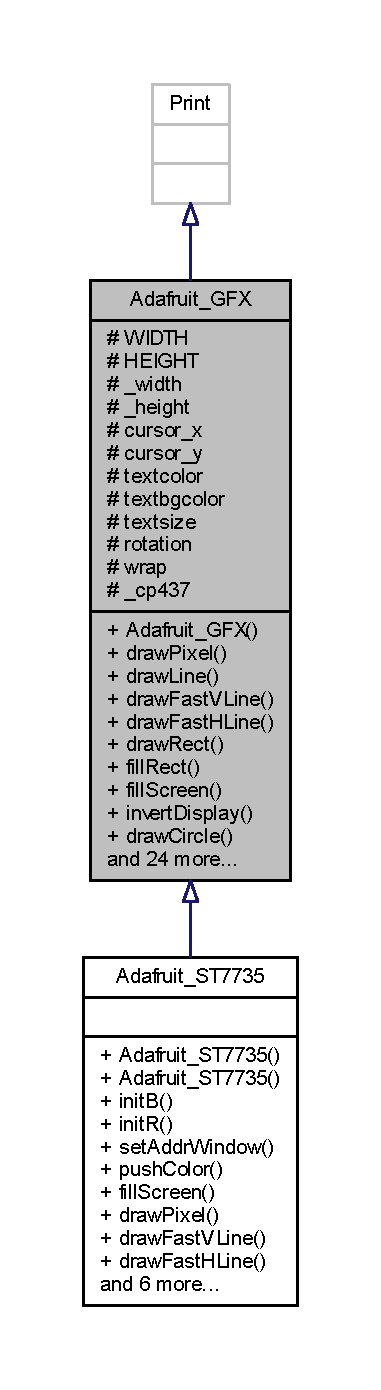
\includegraphics[height=550pt]{df/d49/class_adafruit___g_f_x__inherit__graph}
\end{center}
\end{figure}


Collaboration diagram for Adafruit\+\_\+\+G\+FX\+:
\nopagebreak
\begin{figure}[H]
\begin{center}
\leavevmode
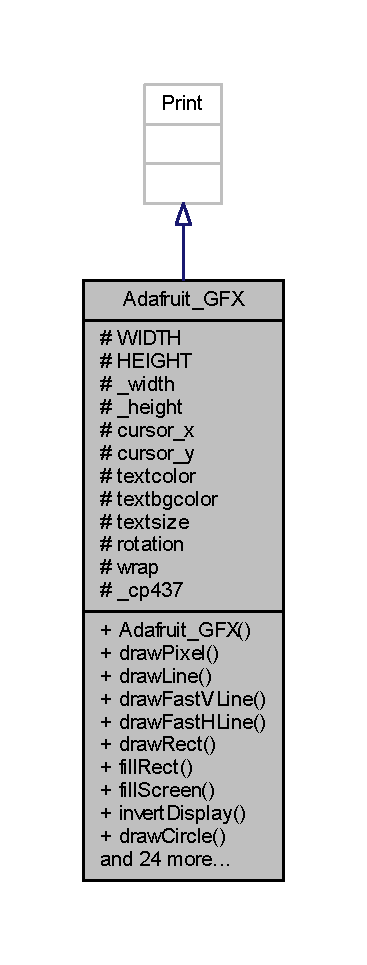
\includegraphics[width=176pt]{d2/d7c/class_adafruit___g_f_x__coll__graph}
\end{center}
\end{figure}
\subsection*{Public Member Functions}
\begin{DoxyCompactItemize}
\item 
\hyperlink{class_adafruit___g_f_x_a6f6f1abccf677eac244fa17d105133ea}{Adafruit\+\_\+\+G\+FX} (int16\+\_\+t w, int16\+\_\+t h)
\item 
virtual void \hyperlink{class_adafruit___g_f_x_ab7fbf72885c873266f9c7eb53b5c8896}{draw\+Pixel} (int16\+\_\+t x, int16\+\_\+t y, uint16\+\_\+t color)=0
\item 
virtual void \hyperlink{class_adafruit___g_f_x_aa0ff662c2b2b48c3bac51f98c777776d}{draw\+Line} (int16\+\_\+t x0, int16\+\_\+t y0, int16\+\_\+t x1, int16\+\_\+t y1, uint16\+\_\+t color)
\item 
virtual void \hyperlink{class_adafruit___g_f_x_a1cffbb1d69c5faf49cd0cff27686a837}{draw\+Fast\+V\+Line} (int16\+\_\+t x, int16\+\_\+t y, int16\+\_\+t h, uint16\+\_\+t color)
\item 
virtual void \hyperlink{class_adafruit___g_f_x_a4d42e7cc577c1eb5b06fe656786c9c79}{draw\+Fast\+H\+Line} (int16\+\_\+t x, int16\+\_\+t y, int16\+\_\+t w, uint16\+\_\+t color)
\item 
virtual void \hyperlink{class_adafruit___g_f_x_a9ec2c2ab426503e4f7deddb93bb916f6}{draw\+Rect} (int16\+\_\+t x, int16\+\_\+t y, int16\+\_\+t w, int16\+\_\+t h, uint16\+\_\+t color)
\item 
virtual void \hyperlink{class_adafruit___g_f_x_aa43cf1dfe6c17d040a0f1fd5ffbe9d69}{fill\+Rect} (int16\+\_\+t x, int16\+\_\+t y, int16\+\_\+t w, int16\+\_\+t h, uint16\+\_\+t color)
\item 
virtual void \hyperlink{class_adafruit___g_f_x_a2b2730aaf2208990928f9c0f85558527}{fill\+Screen} (uint16\+\_\+t color)
\item 
virtual void \hyperlink{class_adafruit___g_f_x_a2fa315803f39a5e73b1841874daf0483}{invert\+Display} (boolean \hyperlink{dac___m_c_p4725_8cpp_ac2e790a754ca79a6e539135dc35f4fc0}{i})
\item 
void \hyperlink{class_adafruit___g_f_x_a648d2d6765e488b4556e802167d885fb}{draw\+Circle} (int16\+\_\+t x0, int16\+\_\+t y0, int16\+\_\+t r, uint16\+\_\+t color)
\item 
void \hyperlink{class_adafruit___g_f_x_a3f2dd7b698e7b95ebf9fecf992ff802e}{draw\+Circle\+Helper} (int16\+\_\+t x0, int16\+\_\+t y0, int16\+\_\+t r, uint8\+\_\+t cornername, uint16\+\_\+t color)
\item 
void \hyperlink{class_adafruit___g_f_x_a623e031e58492fb41e9fde6a05d97c12}{fill\+Circle} (int16\+\_\+t x0, int16\+\_\+t y0, int16\+\_\+t r, uint16\+\_\+t color)
\item 
void \hyperlink{class_adafruit___g_f_x_a2242d3560b08c6480084152b6660052a}{fill\+Circle\+Helper} (int16\+\_\+t x0, int16\+\_\+t y0, int16\+\_\+t r, uint8\+\_\+t cornername, int16\+\_\+t delta, uint16\+\_\+t color)
\item 
void \hyperlink{class_adafruit___g_f_x_a49284b9cea16ecf8c15dfd0b51a841e6}{draw\+Triangle} (int16\+\_\+t x0, int16\+\_\+t y0, int16\+\_\+t x1, int16\+\_\+t y1, int16\+\_\+t x2, int16\+\_\+t y2, uint16\+\_\+t color)
\item 
void \hyperlink{class_adafruit___g_f_x_a4cd646a3d9c9d5b3ee50010d0aa387cd}{fill\+Triangle} (int16\+\_\+t x0, int16\+\_\+t y0, int16\+\_\+t x1, int16\+\_\+t y1, int16\+\_\+t x2, int16\+\_\+t y2, uint16\+\_\+t color)
\item 
void \hyperlink{class_adafruit___g_f_x_ab496b247abec724ef80e17a30257972b}{draw\+Round\+Rect} (int16\+\_\+t x0, int16\+\_\+t y0, int16\+\_\+t w, int16\+\_\+t h, int16\+\_\+t radius, uint16\+\_\+t color)
\item 
void \hyperlink{class_adafruit___g_f_x_a78dc59f6a508bcd3d5ac7af957b8b1ac}{fill\+Round\+Rect} (int16\+\_\+t x0, int16\+\_\+t y0, int16\+\_\+t w, int16\+\_\+t h, int16\+\_\+t radius, uint16\+\_\+t color)
\item 
void \hyperlink{class_adafruit___g_f_x_a50bf54503493152eeefa36f9768acec2}{draw\+Bitmap} (int16\+\_\+t x, int16\+\_\+t y, const uint8\+\_\+t $\ast$bitmap, int16\+\_\+t w, int16\+\_\+t h, uint16\+\_\+t color)
\item 
void \hyperlink{class_adafruit___g_f_x_a5225478b3f2afefcb16ed03e9fe93dc0}{draw\+Bitmap} (int16\+\_\+t x, int16\+\_\+t y, const uint8\+\_\+t $\ast$bitmap, int16\+\_\+t w, int16\+\_\+t h, uint16\+\_\+t color, uint16\+\_\+t bg)
\item 
void \hyperlink{class_adafruit___g_f_x_acec26bcf41c15ac6826c67e1f5e4cde6}{draw\+X\+Bitmap} (int16\+\_\+t x, int16\+\_\+t y, const uint8\+\_\+t $\ast$bitmap, int16\+\_\+t w, int16\+\_\+t h, uint16\+\_\+t color)
\item 
void \hyperlink{class_adafruit___g_f_x_ab7f5a29b3a3dffe30c6a3f4c1f604a5a}{draw\+Char} (int16\+\_\+t x, int16\+\_\+t y, unsigned char c, uint16\+\_\+t color, uint16\+\_\+t bg, uint8\+\_\+t size)
\item 
void \hyperlink{class_adafruit___g_f_x_aaf96a40cad0f34dd8ec73494b3866c33}{set\+Cursor} (int16\+\_\+t x, int16\+\_\+t y)
\item 
void \hyperlink{class_adafruit___g_f_x_a59178a0e0c845a14a39b457c43567dd9}{set\+Text\+Color} (uint16\+\_\+t c)
\item 
void \hyperlink{class_adafruit___g_f_x_ab6e88c585d3ab6b4f95199361f224fc6}{set\+Text\+Color} (uint16\+\_\+t c, uint16\+\_\+t bg)
\item 
void \hyperlink{class_adafruit___g_f_x_a39eb4a8a2c9fa4ab7d58ceffd19535d5}{set\+Text\+Size} (uint8\+\_\+t s)
\item 
void \hyperlink{class_adafruit___g_f_x_aeeacd62bf26f3e7abbdc4b5b50faa6fa}{set\+Text\+Wrap} (boolean w)
\item 
void \hyperlink{class_adafruit___g_f_x_a6ac337c49876cee23ed062a928724675}{set\+Rotation} (uint8\+\_\+t r)
\item 
void \hyperlink{class_adafruit___g_f_x_a6d447fe274e3f0ff12f12afa538d0afe}{cp437} (boolean x=true)
\item 
virtual void \hyperlink{class_adafruit___g_f_x_af4978ea0cf0c0b0540567e82d8fa9900}{write} (uint8\+\_\+t)
\item 
int16\+\_\+t \hyperlink{class_adafruit___g_f_x_a49da524caa19e5202ed2ed7fd5a3baea}{height} (void) const
\item 
int16\+\_\+t \hyperlink{class_adafruit___g_f_x_a324b5361e7198ef0e79eaf4c80bddfc7}{width} (void) const
\item 
uint8\+\_\+t \hyperlink{class_adafruit___g_f_x_ab90e1378511b93189a7b557d7dda5d73}{get\+Rotation} (void) const
\item 
int16\+\_\+t \hyperlink{class_adafruit___g_f_x_a0d1d15f5f15cad95b4c20f0e9ac9c74b}{get\+CursorX} (void) const
\item 
int16\+\_\+t \hyperlink{class_adafruit___g_f_x_a81c8558cfcb717c4cfbd5475998daed1}{get\+CursorY} (void) const
\end{DoxyCompactItemize}
\subsection*{Protected Attributes}
\begin{DoxyCompactItemize}
\item 
const int16\+\_\+t \hyperlink{class_adafruit___g_f_x_ab693a8ac5d94c50c2558b5a3795ddde4}{W\+I\+D\+TH}
\item 
const int16\+\_\+t \hyperlink{class_adafruit___g_f_x_a6b3665babcb73df381563016e9f71bdb}{H\+E\+I\+G\+HT}
\item 
int16\+\_\+t \hyperlink{class_adafruit___g_f_x_ab237f850a033492f5e745d79405a097a}{\+\_\+width}
\item 
int16\+\_\+t \hyperlink{class_adafruit___g_f_x_ab9bb0cbc2455f64dce2a5ec36307aa94}{\+\_\+height}
\item 
int16\+\_\+t \hyperlink{class_adafruit___g_f_x_a8f8983cea8d81a7c8e9d05eef36318e2}{cursor\+\_\+x}
\item 
int16\+\_\+t \hyperlink{class_adafruit___g_f_x_aebe0a38f6e6fd59cb81620c4696286c9}{cursor\+\_\+y}
\item 
uint16\+\_\+t \hyperlink{class_adafruit___g_f_x_a8c6d23a386651136fd9530a5b7046591}{textcolor}
\item 
uint16\+\_\+t \hyperlink{class_adafruit___g_f_x_a23e7a4efcab0b1588dc0cafa14b1fac1}{textbgcolor}
\item 
uint8\+\_\+t \hyperlink{class_adafruit___g_f_x_ac293848b8fe8c46107d1a491f6a5168d}{textsize}
\item 
uint8\+\_\+t \hyperlink{class_adafruit___g_f_x_a37a479d28fb11906ce516e983b1af926}{rotation}
\item 
boolean \hyperlink{class_adafruit___g_f_x_ad6bd603e01861212829d536312a7190b}{wrap}
\item 
boolean \hyperlink{class_adafruit___g_f_x_aaef3d4d239641084cd3825a8b1042e01}{\+\_\+cp437}
\end{DoxyCompactItemize}


\subsection{Constructor \& Destructor Documentation}
\mbox{\Hypertarget{class_adafruit___g_f_x_a6f6f1abccf677eac244fa17d105133ea}\label{class_adafruit___g_f_x_a6f6f1abccf677eac244fa17d105133ea}} 
\index{Adafruit\+\_\+\+G\+FX@{Adafruit\+\_\+\+G\+FX}!Adafruit\+\_\+\+G\+FX@{Adafruit\+\_\+\+G\+FX}}
\index{Adafruit\+\_\+\+G\+FX@{Adafruit\+\_\+\+G\+FX}!Adafruit\+\_\+\+G\+FX@{Adafruit\+\_\+\+G\+FX}}
\subsubsection{\texorpdfstring{Adafruit\+\_\+\+G\+F\+X()}{Adafruit\_GFX()}}
{\footnotesize\ttfamily Adafruit\+\_\+\+G\+F\+X\+::\+Adafruit\+\_\+\+G\+FX (\begin{DoxyParamCaption}\item[{int16\+\_\+t}]{w,  }\item[{int16\+\_\+t}]{h }\end{DoxyParamCaption})}



\subsection{Member Function Documentation}
\mbox{\Hypertarget{class_adafruit___g_f_x_a6d447fe274e3f0ff12f12afa538d0afe}\label{class_adafruit___g_f_x_a6d447fe274e3f0ff12f12afa538d0afe}} 
\index{Adafruit\+\_\+\+G\+FX@{Adafruit\+\_\+\+G\+FX}!cp437@{cp437}}
\index{cp437@{cp437}!Adafruit\+\_\+\+G\+FX@{Adafruit\+\_\+\+G\+FX}}
\subsubsection{\texorpdfstring{cp437()}{cp437()}}
{\footnotesize\ttfamily void Adafruit\+\_\+\+G\+F\+X\+::cp437 (\begin{DoxyParamCaption}\item[{boolean}]{x = {\ttfamily true} }\end{DoxyParamCaption})}

\mbox{\Hypertarget{class_adafruit___g_f_x_a50bf54503493152eeefa36f9768acec2}\label{class_adafruit___g_f_x_a50bf54503493152eeefa36f9768acec2}} 
\index{Adafruit\+\_\+\+G\+FX@{Adafruit\+\_\+\+G\+FX}!draw\+Bitmap@{draw\+Bitmap}}
\index{draw\+Bitmap@{draw\+Bitmap}!Adafruit\+\_\+\+G\+FX@{Adafruit\+\_\+\+G\+FX}}
\subsubsection{\texorpdfstring{draw\+Bitmap()}{drawBitmap()}\hspace{0.1cm}{\footnotesize\ttfamily [1/2]}}
{\footnotesize\ttfamily void Adafruit\+\_\+\+G\+F\+X\+::draw\+Bitmap (\begin{DoxyParamCaption}\item[{int16\+\_\+t}]{x,  }\item[{int16\+\_\+t}]{y,  }\item[{const uint8\+\_\+t $\ast$}]{bitmap,  }\item[{int16\+\_\+t}]{w,  }\item[{int16\+\_\+t}]{h,  }\item[{uint16\+\_\+t}]{color }\end{DoxyParamCaption})}

Here is the call graph for this function\+:
\nopagebreak
\begin{figure}[H]
\begin{center}
\leavevmode
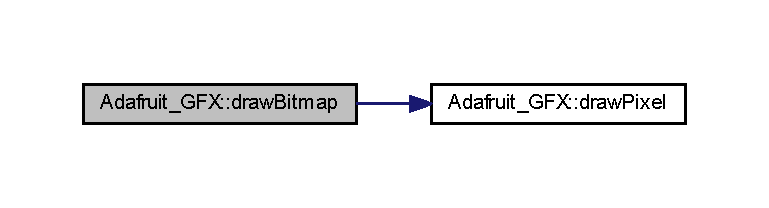
\includegraphics[width=350pt]{d9/d97/class_adafruit___g_f_x_a50bf54503493152eeefa36f9768acec2_cgraph}
\end{center}
\end{figure}
\mbox{\Hypertarget{class_adafruit___g_f_x_a5225478b3f2afefcb16ed03e9fe93dc0}\label{class_adafruit___g_f_x_a5225478b3f2afefcb16ed03e9fe93dc0}} 
\index{Adafruit\+\_\+\+G\+FX@{Adafruit\+\_\+\+G\+FX}!draw\+Bitmap@{draw\+Bitmap}}
\index{draw\+Bitmap@{draw\+Bitmap}!Adafruit\+\_\+\+G\+FX@{Adafruit\+\_\+\+G\+FX}}
\subsubsection{\texorpdfstring{draw\+Bitmap()}{drawBitmap()}\hspace{0.1cm}{\footnotesize\ttfamily [2/2]}}
{\footnotesize\ttfamily void Adafruit\+\_\+\+G\+F\+X\+::draw\+Bitmap (\begin{DoxyParamCaption}\item[{int16\+\_\+t}]{x,  }\item[{int16\+\_\+t}]{y,  }\item[{const uint8\+\_\+t $\ast$}]{bitmap,  }\item[{int16\+\_\+t}]{w,  }\item[{int16\+\_\+t}]{h,  }\item[{uint16\+\_\+t}]{color,  }\item[{uint16\+\_\+t}]{bg }\end{DoxyParamCaption})}

Here is the call graph for this function\+:
\nopagebreak
\begin{figure}[H]
\begin{center}
\leavevmode
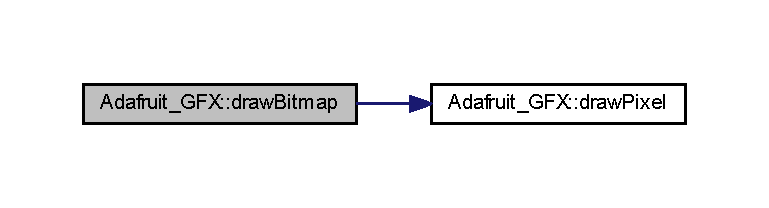
\includegraphics[width=350pt]{d9/d97/class_adafruit___g_f_x_a5225478b3f2afefcb16ed03e9fe93dc0_cgraph}
\end{center}
\end{figure}
\mbox{\Hypertarget{class_adafruit___g_f_x_ab7f5a29b3a3dffe30c6a3f4c1f604a5a}\label{class_adafruit___g_f_x_ab7f5a29b3a3dffe30c6a3f4c1f604a5a}} 
\index{Adafruit\+\_\+\+G\+FX@{Adafruit\+\_\+\+G\+FX}!draw\+Char@{draw\+Char}}
\index{draw\+Char@{draw\+Char}!Adafruit\+\_\+\+G\+FX@{Adafruit\+\_\+\+G\+FX}}
\subsubsection{\texorpdfstring{draw\+Char()}{drawChar()}}
{\footnotesize\ttfamily void Adafruit\+\_\+\+G\+F\+X\+::draw\+Char (\begin{DoxyParamCaption}\item[{int16\+\_\+t}]{x,  }\item[{int16\+\_\+t}]{y,  }\item[{unsigned char}]{c,  }\item[{uint16\+\_\+t}]{color,  }\item[{uint16\+\_\+t}]{bg,  }\item[{uint8\+\_\+t}]{size }\end{DoxyParamCaption})}

Here is the call graph for this function\+:
\nopagebreak
\begin{figure}[H]
\begin{center}
\leavevmode
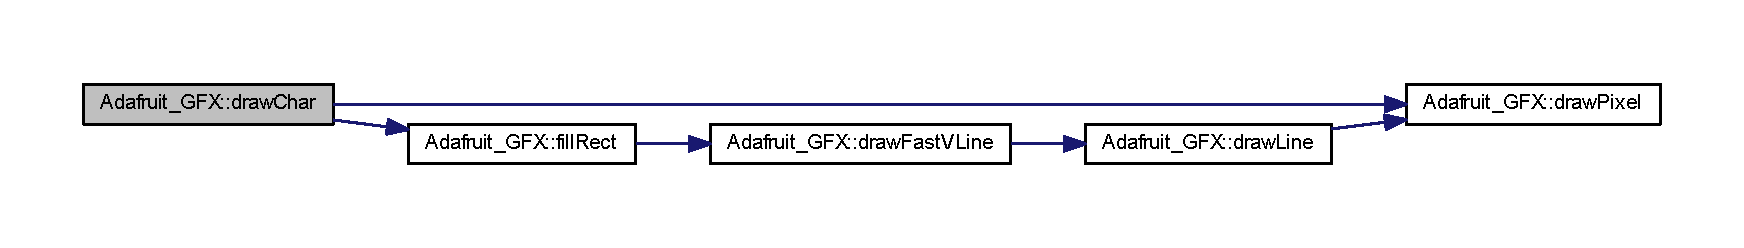
\includegraphics[width=350pt]{d9/d97/class_adafruit___g_f_x_ab7f5a29b3a3dffe30c6a3f4c1f604a5a_cgraph}
\end{center}
\end{figure}
Here is the caller graph for this function\+:
\nopagebreak
\begin{figure}[H]
\begin{center}
\leavevmode
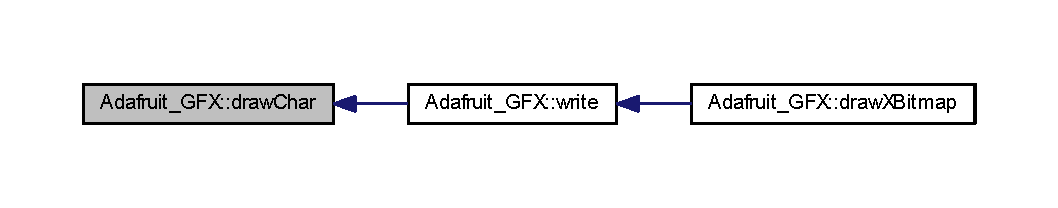
\includegraphics[width=350pt]{d9/d97/class_adafruit___g_f_x_ab7f5a29b3a3dffe30c6a3f4c1f604a5a_icgraph}
\end{center}
\end{figure}
\mbox{\Hypertarget{class_adafruit___g_f_x_a648d2d6765e488b4556e802167d885fb}\label{class_adafruit___g_f_x_a648d2d6765e488b4556e802167d885fb}} 
\index{Adafruit\+\_\+\+G\+FX@{Adafruit\+\_\+\+G\+FX}!draw\+Circle@{draw\+Circle}}
\index{draw\+Circle@{draw\+Circle}!Adafruit\+\_\+\+G\+FX@{Adafruit\+\_\+\+G\+FX}}
\subsubsection{\texorpdfstring{draw\+Circle()}{drawCircle()}}
{\footnotesize\ttfamily void Adafruit\+\_\+\+G\+F\+X\+::draw\+Circle (\begin{DoxyParamCaption}\item[{int16\+\_\+t}]{x0,  }\item[{int16\+\_\+t}]{y0,  }\item[{int16\+\_\+t}]{r,  }\item[{uint16\+\_\+t}]{color }\end{DoxyParamCaption})}

Here is the call graph for this function\+:
\nopagebreak
\begin{figure}[H]
\begin{center}
\leavevmode
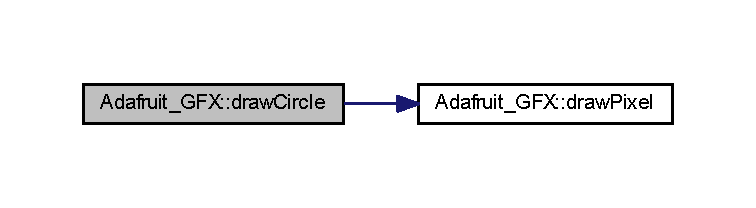
\includegraphics[width=350pt]{d9/d97/class_adafruit___g_f_x_a648d2d6765e488b4556e802167d885fb_cgraph}
\end{center}
\end{figure}
\mbox{\Hypertarget{class_adafruit___g_f_x_a3f2dd7b698e7b95ebf9fecf992ff802e}\label{class_adafruit___g_f_x_a3f2dd7b698e7b95ebf9fecf992ff802e}} 
\index{Adafruit\+\_\+\+G\+FX@{Adafruit\+\_\+\+G\+FX}!draw\+Circle\+Helper@{draw\+Circle\+Helper}}
\index{draw\+Circle\+Helper@{draw\+Circle\+Helper}!Adafruit\+\_\+\+G\+FX@{Adafruit\+\_\+\+G\+FX}}
\subsubsection{\texorpdfstring{draw\+Circle\+Helper()}{drawCircleHelper()}}
{\footnotesize\ttfamily void Adafruit\+\_\+\+G\+F\+X\+::draw\+Circle\+Helper (\begin{DoxyParamCaption}\item[{int16\+\_\+t}]{x0,  }\item[{int16\+\_\+t}]{y0,  }\item[{int16\+\_\+t}]{r,  }\item[{uint8\+\_\+t}]{cornername,  }\item[{uint16\+\_\+t}]{color }\end{DoxyParamCaption})}

Here is the call graph for this function\+:
\nopagebreak
\begin{figure}[H]
\begin{center}
\leavevmode
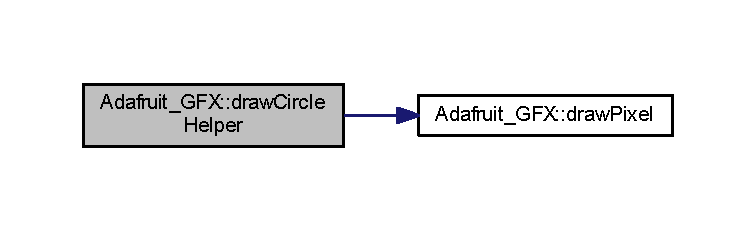
\includegraphics[width=350pt]{d9/d97/class_adafruit___g_f_x_a3f2dd7b698e7b95ebf9fecf992ff802e_cgraph}
\end{center}
\end{figure}
Here is the caller graph for this function\+:
\nopagebreak
\begin{figure}[H]
\begin{center}
\leavevmode
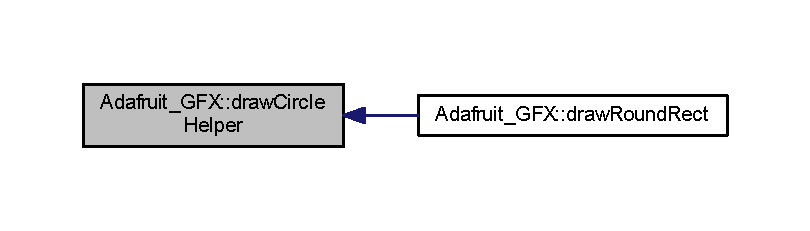
\includegraphics[width=350pt]{d9/d97/class_adafruit___g_f_x_a3f2dd7b698e7b95ebf9fecf992ff802e_icgraph}
\end{center}
\end{figure}
\mbox{\Hypertarget{class_adafruit___g_f_x_a4d42e7cc577c1eb5b06fe656786c9c79}\label{class_adafruit___g_f_x_a4d42e7cc577c1eb5b06fe656786c9c79}} 
\index{Adafruit\+\_\+\+G\+FX@{Adafruit\+\_\+\+G\+FX}!draw\+Fast\+H\+Line@{draw\+Fast\+H\+Line}}
\index{draw\+Fast\+H\+Line@{draw\+Fast\+H\+Line}!Adafruit\+\_\+\+G\+FX@{Adafruit\+\_\+\+G\+FX}}
\subsubsection{\texorpdfstring{draw\+Fast\+H\+Line()}{drawFastHLine()}}
{\footnotesize\ttfamily void Adafruit\+\_\+\+G\+F\+X\+::draw\+Fast\+H\+Line (\begin{DoxyParamCaption}\item[{int16\+\_\+t}]{x,  }\item[{int16\+\_\+t}]{y,  }\item[{int16\+\_\+t}]{w,  }\item[{uint16\+\_\+t}]{color }\end{DoxyParamCaption})}

Here is the call graph for this function\+:
\nopagebreak
\begin{figure}[H]
\begin{center}
\leavevmode
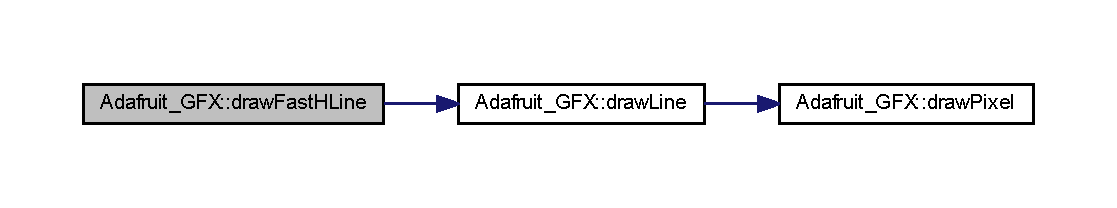
\includegraphics[width=350pt]{d9/d97/class_adafruit___g_f_x_a4d42e7cc577c1eb5b06fe656786c9c79_cgraph}
\end{center}
\end{figure}
Here is the caller graph for this function\+:
\nopagebreak
\begin{figure}[H]
\begin{center}
\leavevmode
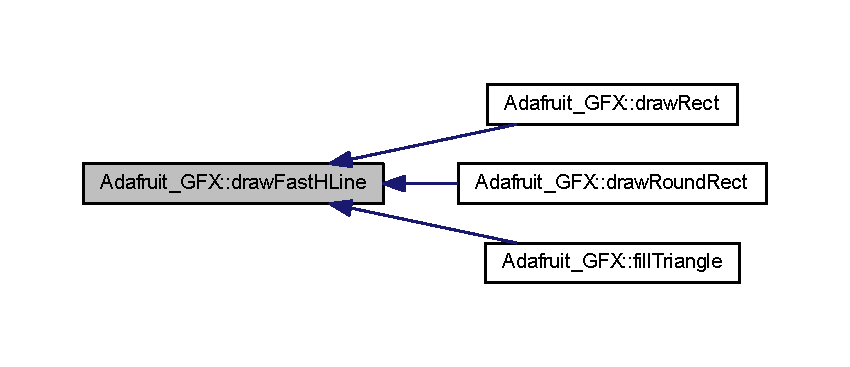
\includegraphics[width=350pt]{d9/d97/class_adafruit___g_f_x_a4d42e7cc577c1eb5b06fe656786c9c79_icgraph}
\end{center}
\end{figure}
\mbox{\Hypertarget{class_adafruit___g_f_x_a1cffbb1d69c5faf49cd0cff27686a837}\label{class_adafruit___g_f_x_a1cffbb1d69c5faf49cd0cff27686a837}} 
\index{Adafruit\+\_\+\+G\+FX@{Adafruit\+\_\+\+G\+FX}!draw\+Fast\+V\+Line@{draw\+Fast\+V\+Line}}
\index{draw\+Fast\+V\+Line@{draw\+Fast\+V\+Line}!Adafruit\+\_\+\+G\+FX@{Adafruit\+\_\+\+G\+FX}}
\subsubsection{\texorpdfstring{draw\+Fast\+V\+Line()}{drawFastVLine()}}
{\footnotesize\ttfamily void Adafruit\+\_\+\+G\+F\+X\+::draw\+Fast\+V\+Line (\begin{DoxyParamCaption}\item[{int16\+\_\+t}]{x,  }\item[{int16\+\_\+t}]{y,  }\item[{int16\+\_\+t}]{h,  }\item[{uint16\+\_\+t}]{color }\end{DoxyParamCaption})}

Here is the call graph for this function\+:
\nopagebreak
\begin{figure}[H]
\begin{center}
\leavevmode
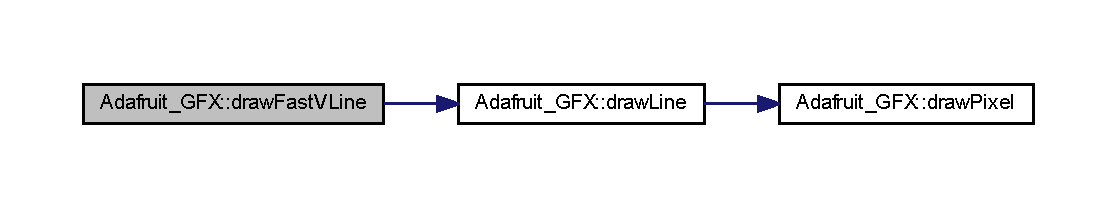
\includegraphics[width=350pt]{d9/d97/class_adafruit___g_f_x_a1cffbb1d69c5faf49cd0cff27686a837_cgraph}
\end{center}
\end{figure}
Here is the caller graph for this function\+:
\nopagebreak
\begin{figure}[H]
\begin{center}
\leavevmode
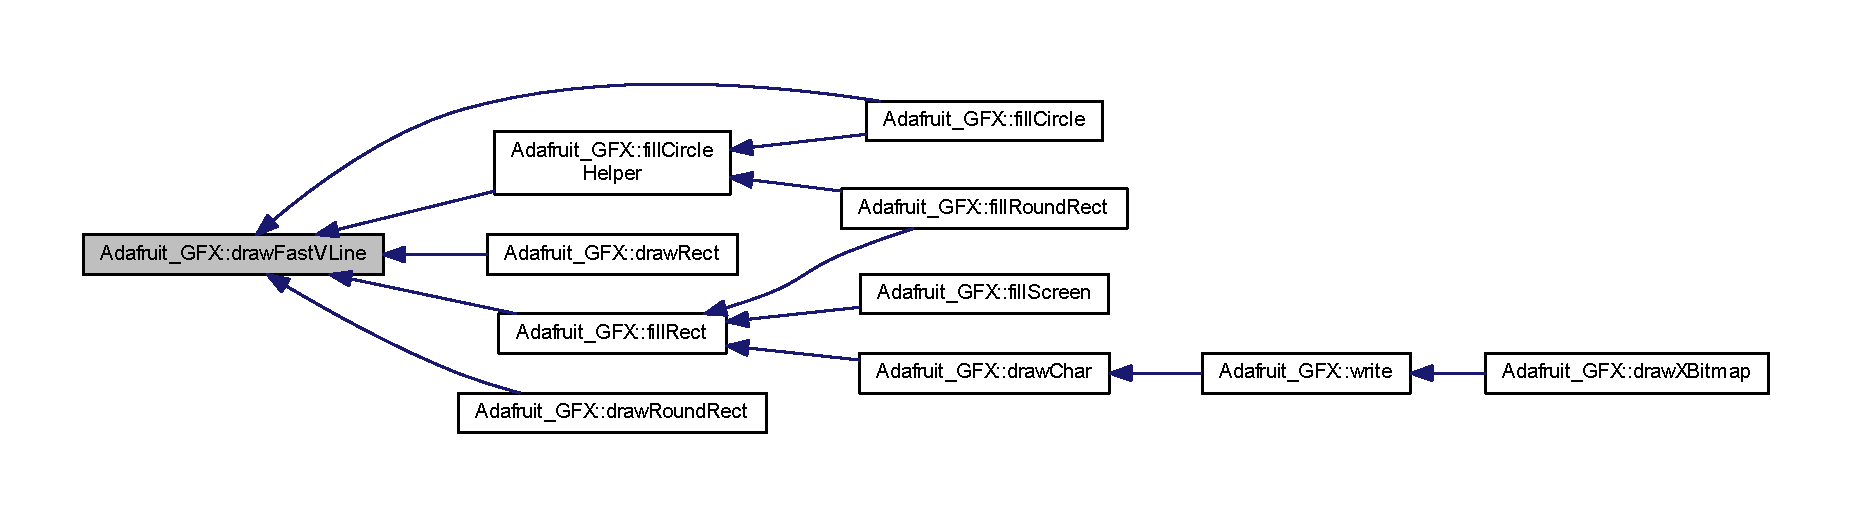
\includegraphics[width=350pt]{d9/d97/class_adafruit___g_f_x_a1cffbb1d69c5faf49cd0cff27686a837_icgraph}
\end{center}
\end{figure}
\mbox{\Hypertarget{class_adafruit___g_f_x_aa0ff662c2b2b48c3bac51f98c777776d}\label{class_adafruit___g_f_x_aa0ff662c2b2b48c3bac51f98c777776d}} 
\index{Adafruit\+\_\+\+G\+FX@{Adafruit\+\_\+\+G\+FX}!draw\+Line@{draw\+Line}}
\index{draw\+Line@{draw\+Line}!Adafruit\+\_\+\+G\+FX@{Adafruit\+\_\+\+G\+FX}}
\subsubsection{\texorpdfstring{draw\+Line()}{drawLine()}}
{\footnotesize\ttfamily void Adafruit\+\_\+\+G\+F\+X\+::draw\+Line (\begin{DoxyParamCaption}\item[{int16\+\_\+t}]{x0,  }\item[{int16\+\_\+t}]{y0,  }\item[{int16\+\_\+t}]{x1,  }\item[{int16\+\_\+t}]{y1,  }\item[{uint16\+\_\+t}]{color }\end{DoxyParamCaption})\hspace{0.3cm}{\ttfamily [virtual]}}

Here is the call graph for this function\+:
\nopagebreak
\begin{figure}[H]
\begin{center}
\leavevmode
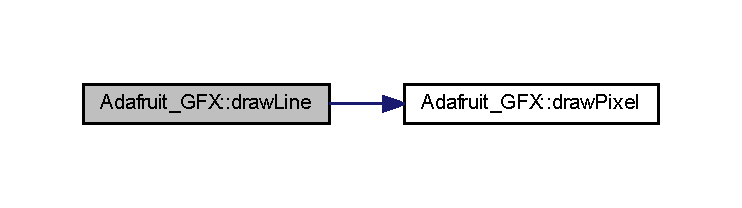
\includegraphics[width=350pt]{d9/d97/class_adafruit___g_f_x_aa0ff662c2b2b48c3bac51f98c777776d_cgraph}
\end{center}
\end{figure}
Here is the caller graph for this function\+:
\nopagebreak
\begin{figure}[H]
\begin{center}
\leavevmode
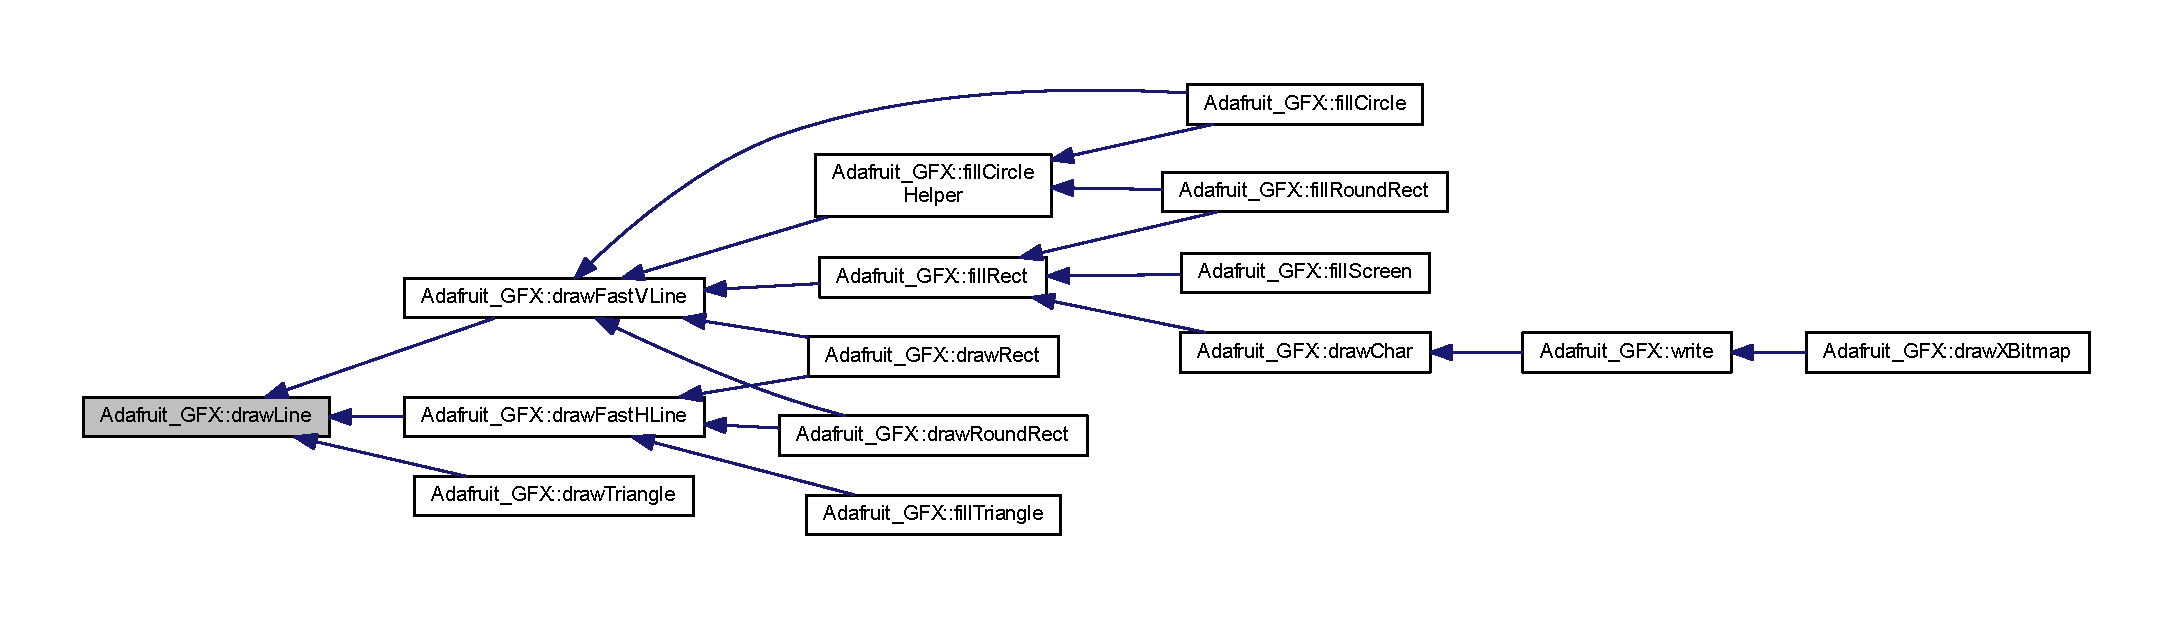
\includegraphics[width=350pt]{d9/d97/class_adafruit___g_f_x_aa0ff662c2b2b48c3bac51f98c777776d_icgraph}
\end{center}
\end{figure}
\mbox{\Hypertarget{class_adafruit___g_f_x_ab7fbf72885c873266f9c7eb53b5c8896}\label{class_adafruit___g_f_x_ab7fbf72885c873266f9c7eb53b5c8896}} 
\index{Adafruit\+\_\+\+G\+FX@{Adafruit\+\_\+\+G\+FX}!draw\+Pixel@{draw\+Pixel}}
\index{draw\+Pixel@{draw\+Pixel}!Adafruit\+\_\+\+G\+FX@{Adafruit\+\_\+\+G\+FX}}
\subsubsection{\texorpdfstring{draw\+Pixel()}{drawPixel()}}
{\footnotesize\ttfamily virtual void Adafruit\+\_\+\+G\+F\+X\+::draw\+Pixel (\begin{DoxyParamCaption}\item[{int16\+\_\+t}]{x,  }\item[{int16\+\_\+t}]{y,  }\item[{uint16\+\_\+t}]{color }\end{DoxyParamCaption})\hspace{0.3cm}{\ttfamily [pure virtual]}}



Implemented in \hyperlink{class_adafruit___s_t7735_af22a5ba7282850793f4943ba2d682af0}{Adafruit\+\_\+\+S\+T7735}.

Here is the caller graph for this function\+:
\nopagebreak
\begin{figure}[H]
\begin{center}
\leavevmode
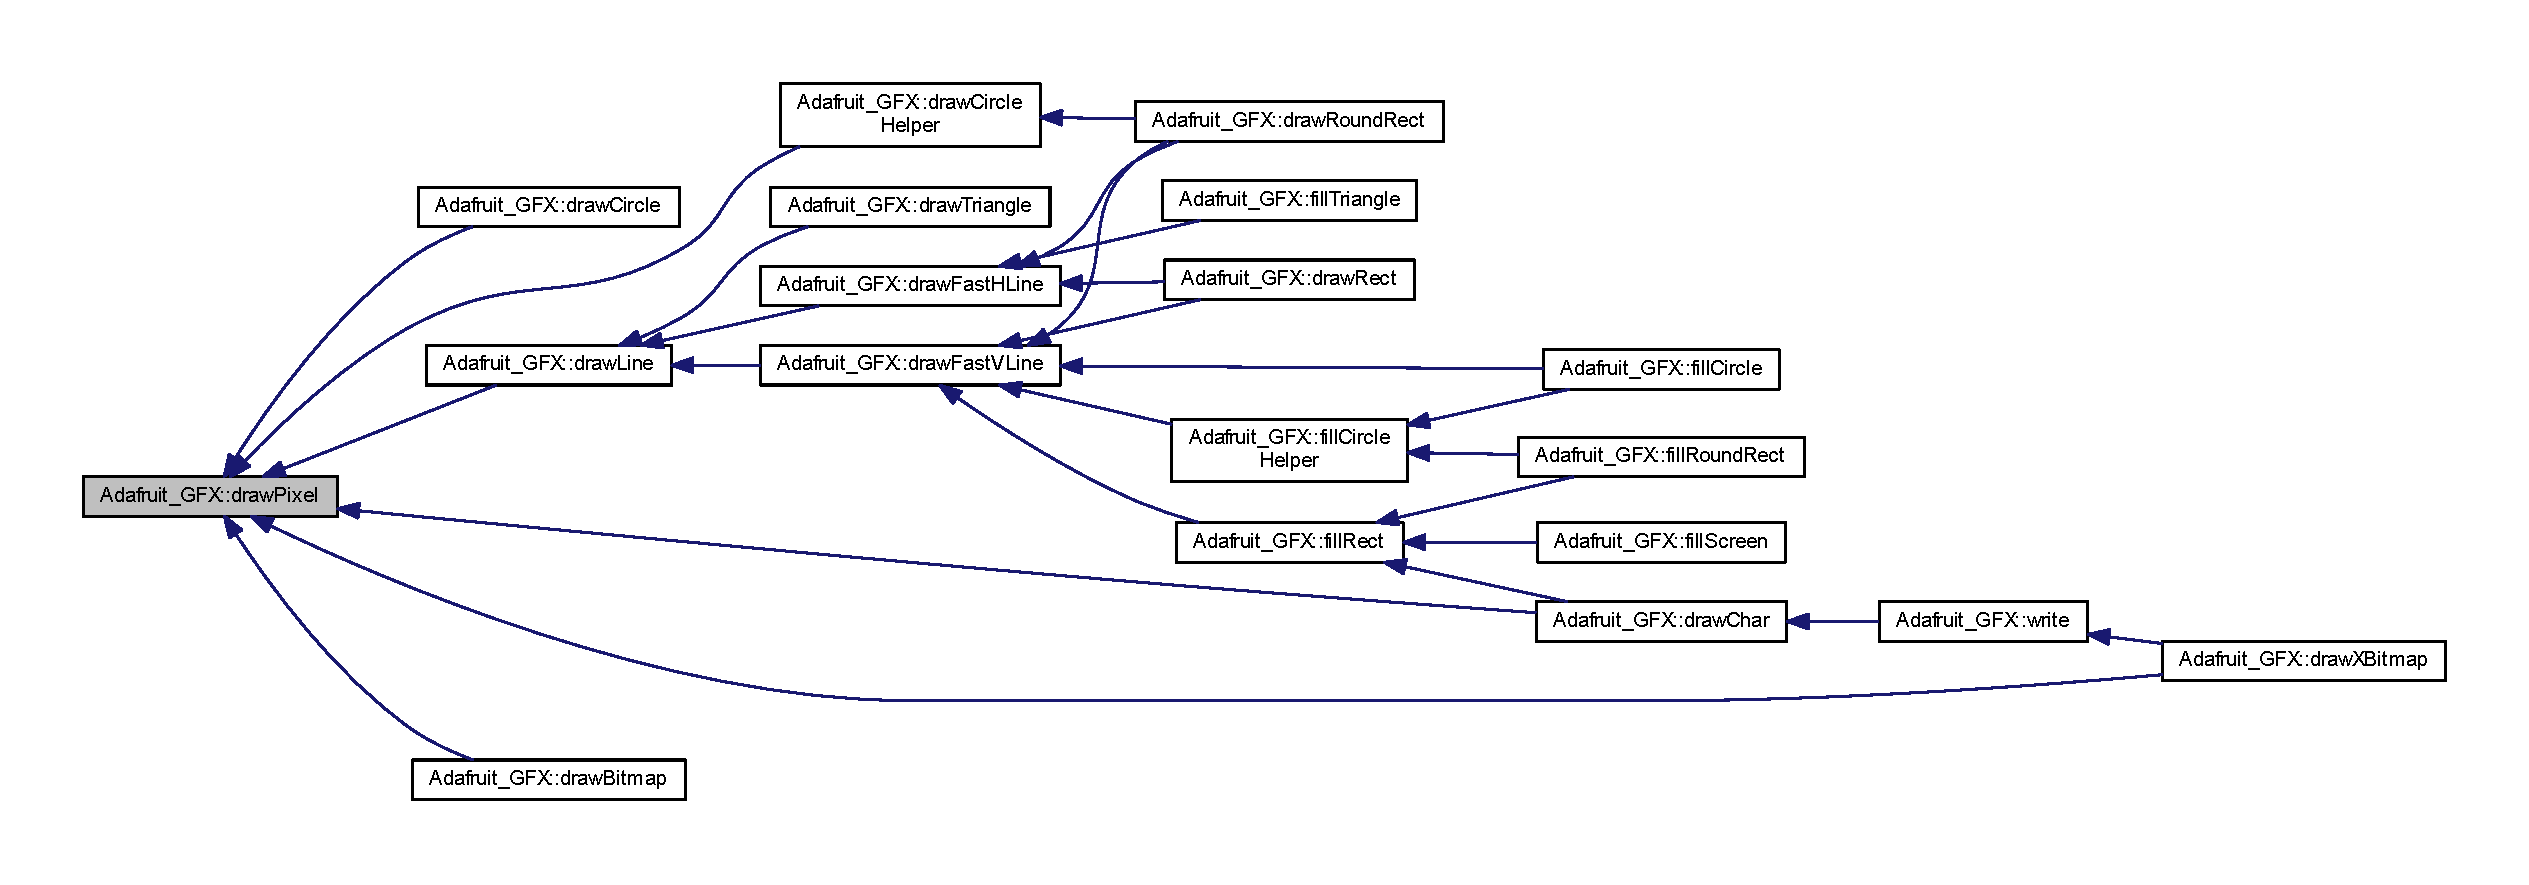
\includegraphics[width=350pt]{d9/d97/class_adafruit___g_f_x_ab7fbf72885c873266f9c7eb53b5c8896_icgraph}
\end{center}
\end{figure}
\mbox{\Hypertarget{class_adafruit___g_f_x_a9ec2c2ab426503e4f7deddb93bb916f6}\label{class_adafruit___g_f_x_a9ec2c2ab426503e4f7deddb93bb916f6}} 
\index{Adafruit\+\_\+\+G\+FX@{Adafruit\+\_\+\+G\+FX}!draw\+Rect@{draw\+Rect}}
\index{draw\+Rect@{draw\+Rect}!Adafruit\+\_\+\+G\+FX@{Adafruit\+\_\+\+G\+FX}}
\subsubsection{\texorpdfstring{draw\+Rect()}{drawRect()}}
{\footnotesize\ttfamily void Adafruit\+\_\+\+G\+F\+X\+::draw\+Rect (\begin{DoxyParamCaption}\item[{int16\+\_\+t}]{x,  }\item[{int16\+\_\+t}]{y,  }\item[{int16\+\_\+t}]{w,  }\item[{int16\+\_\+t}]{h,  }\item[{uint16\+\_\+t}]{color }\end{DoxyParamCaption})}

Here is the call graph for this function\+:
\nopagebreak
\begin{figure}[H]
\begin{center}
\leavevmode
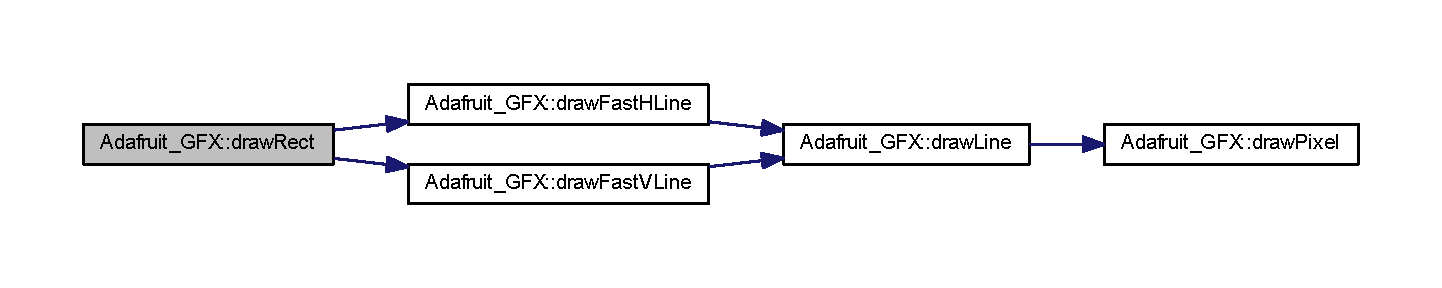
\includegraphics[width=350pt]{d9/d97/class_adafruit___g_f_x_a9ec2c2ab426503e4f7deddb93bb916f6_cgraph}
\end{center}
\end{figure}
\mbox{\Hypertarget{class_adafruit___g_f_x_ab496b247abec724ef80e17a30257972b}\label{class_adafruit___g_f_x_ab496b247abec724ef80e17a30257972b}} 
\index{Adafruit\+\_\+\+G\+FX@{Adafruit\+\_\+\+G\+FX}!draw\+Round\+Rect@{draw\+Round\+Rect}}
\index{draw\+Round\+Rect@{draw\+Round\+Rect}!Adafruit\+\_\+\+G\+FX@{Adafruit\+\_\+\+G\+FX}}
\subsubsection{\texorpdfstring{draw\+Round\+Rect()}{drawRoundRect()}}
{\footnotesize\ttfamily void Adafruit\+\_\+\+G\+F\+X\+::draw\+Round\+Rect (\begin{DoxyParamCaption}\item[{int16\+\_\+t}]{x0,  }\item[{int16\+\_\+t}]{y0,  }\item[{int16\+\_\+t}]{w,  }\item[{int16\+\_\+t}]{h,  }\item[{int16\+\_\+t}]{radius,  }\item[{uint16\+\_\+t}]{color }\end{DoxyParamCaption})}

Here is the call graph for this function\+:
\nopagebreak
\begin{figure}[H]
\begin{center}
\leavevmode
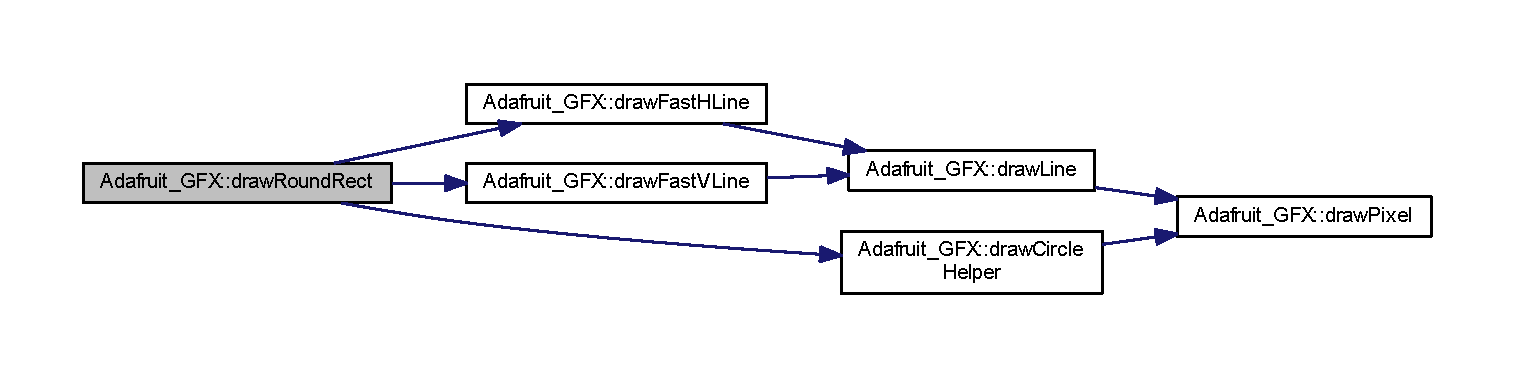
\includegraphics[width=350pt]{d9/d97/class_adafruit___g_f_x_ab496b247abec724ef80e17a30257972b_cgraph}
\end{center}
\end{figure}
\mbox{\Hypertarget{class_adafruit___g_f_x_a49284b9cea16ecf8c15dfd0b51a841e6}\label{class_adafruit___g_f_x_a49284b9cea16ecf8c15dfd0b51a841e6}} 
\index{Adafruit\+\_\+\+G\+FX@{Adafruit\+\_\+\+G\+FX}!draw\+Triangle@{draw\+Triangle}}
\index{draw\+Triangle@{draw\+Triangle}!Adafruit\+\_\+\+G\+FX@{Adafruit\+\_\+\+G\+FX}}
\subsubsection{\texorpdfstring{draw\+Triangle()}{drawTriangle()}}
{\footnotesize\ttfamily void Adafruit\+\_\+\+G\+F\+X\+::draw\+Triangle (\begin{DoxyParamCaption}\item[{int16\+\_\+t}]{x0,  }\item[{int16\+\_\+t}]{y0,  }\item[{int16\+\_\+t}]{x1,  }\item[{int16\+\_\+t}]{y1,  }\item[{int16\+\_\+t}]{x2,  }\item[{int16\+\_\+t}]{y2,  }\item[{uint16\+\_\+t}]{color }\end{DoxyParamCaption})}

Here is the call graph for this function\+:
\nopagebreak
\begin{figure}[H]
\begin{center}
\leavevmode
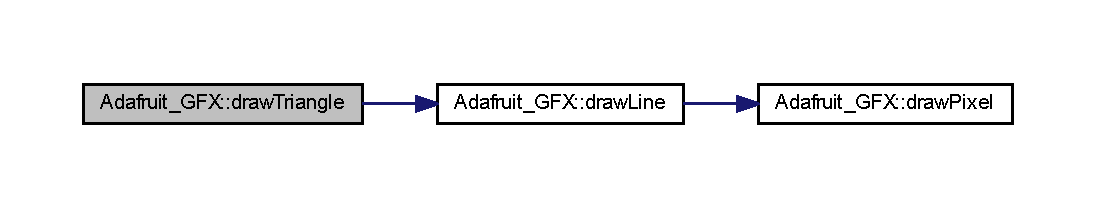
\includegraphics[width=350pt]{d9/d97/class_adafruit___g_f_x_a49284b9cea16ecf8c15dfd0b51a841e6_cgraph}
\end{center}
\end{figure}
\mbox{\Hypertarget{class_adafruit___g_f_x_acec26bcf41c15ac6826c67e1f5e4cde6}\label{class_adafruit___g_f_x_acec26bcf41c15ac6826c67e1f5e4cde6}} 
\index{Adafruit\+\_\+\+G\+FX@{Adafruit\+\_\+\+G\+FX}!draw\+X\+Bitmap@{draw\+X\+Bitmap}}
\index{draw\+X\+Bitmap@{draw\+X\+Bitmap}!Adafruit\+\_\+\+G\+FX@{Adafruit\+\_\+\+G\+FX}}
\subsubsection{\texorpdfstring{draw\+X\+Bitmap()}{drawXBitmap()}}
{\footnotesize\ttfamily void Adafruit\+\_\+\+G\+F\+X\+::draw\+X\+Bitmap (\begin{DoxyParamCaption}\item[{int16\+\_\+t}]{x,  }\item[{int16\+\_\+t}]{y,  }\item[{const uint8\+\_\+t $\ast$}]{bitmap,  }\item[{int16\+\_\+t}]{w,  }\item[{int16\+\_\+t}]{h,  }\item[{uint16\+\_\+t}]{color }\end{DoxyParamCaption})}

Here is the call graph for this function\+:
\nopagebreak
\begin{figure}[H]
\begin{center}
\leavevmode
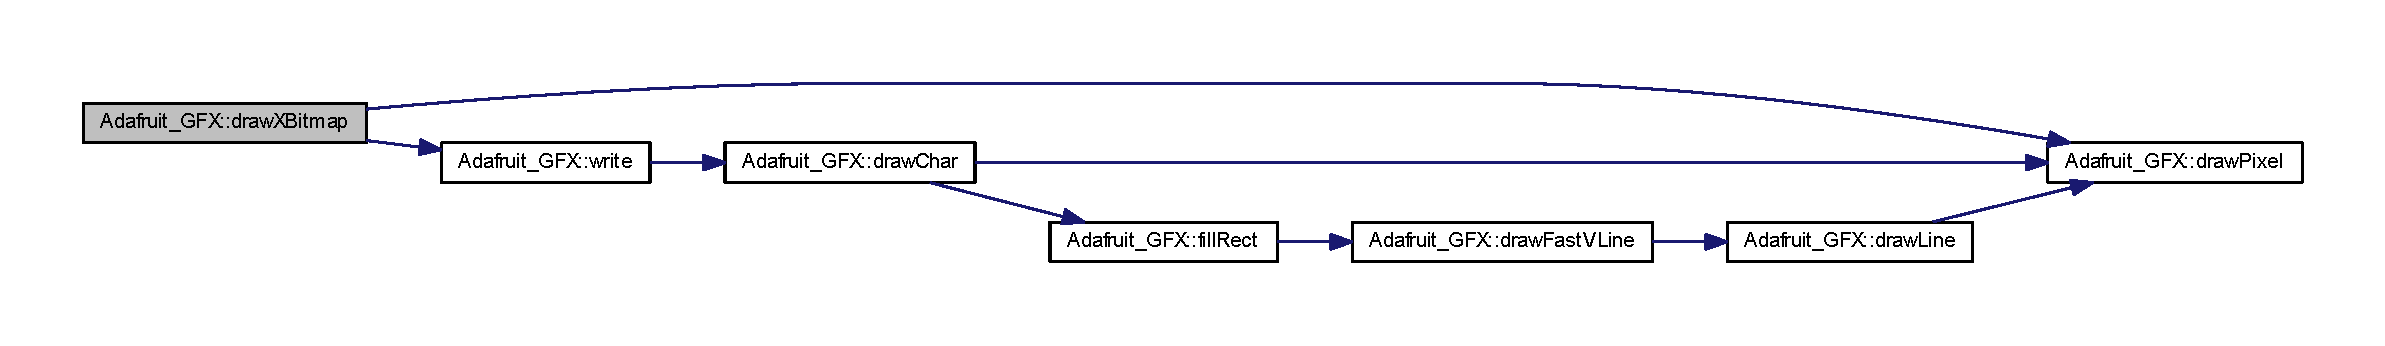
\includegraphics[width=350pt]{d9/d97/class_adafruit___g_f_x_acec26bcf41c15ac6826c67e1f5e4cde6_cgraph}
\end{center}
\end{figure}
\mbox{\Hypertarget{class_adafruit___g_f_x_a623e031e58492fb41e9fde6a05d97c12}\label{class_adafruit___g_f_x_a623e031e58492fb41e9fde6a05d97c12}} 
\index{Adafruit\+\_\+\+G\+FX@{Adafruit\+\_\+\+G\+FX}!fill\+Circle@{fill\+Circle}}
\index{fill\+Circle@{fill\+Circle}!Adafruit\+\_\+\+G\+FX@{Adafruit\+\_\+\+G\+FX}}
\subsubsection{\texorpdfstring{fill\+Circle()}{fillCircle()}}
{\footnotesize\ttfamily void Adafruit\+\_\+\+G\+F\+X\+::fill\+Circle (\begin{DoxyParamCaption}\item[{int16\+\_\+t}]{x0,  }\item[{int16\+\_\+t}]{y0,  }\item[{int16\+\_\+t}]{r,  }\item[{uint16\+\_\+t}]{color }\end{DoxyParamCaption})}

Here is the call graph for this function\+:
\nopagebreak
\begin{figure}[H]
\begin{center}
\leavevmode
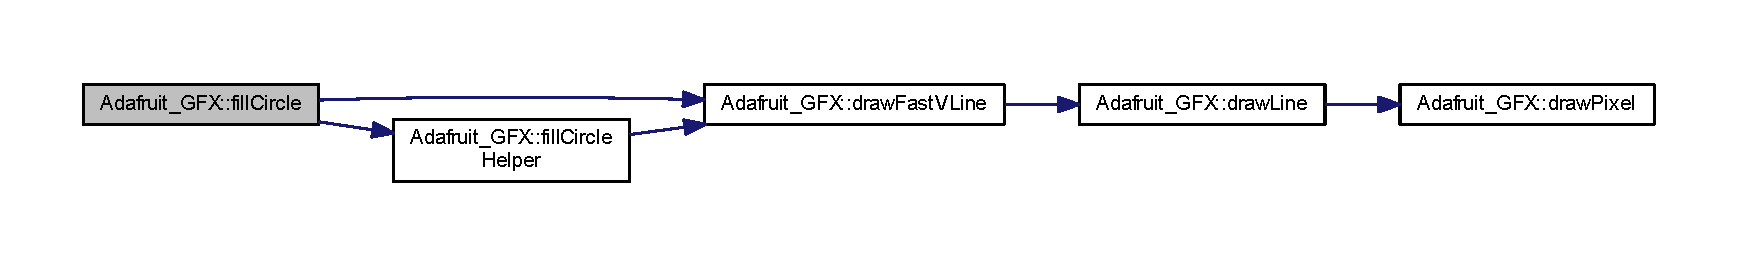
\includegraphics[width=350pt]{d9/d97/class_adafruit___g_f_x_a623e031e58492fb41e9fde6a05d97c12_cgraph}
\end{center}
\end{figure}
\mbox{\Hypertarget{class_adafruit___g_f_x_a2242d3560b08c6480084152b6660052a}\label{class_adafruit___g_f_x_a2242d3560b08c6480084152b6660052a}} 
\index{Adafruit\+\_\+\+G\+FX@{Adafruit\+\_\+\+G\+FX}!fill\+Circle\+Helper@{fill\+Circle\+Helper}}
\index{fill\+Circle\+Helper@{fill\+Circle\+Helper}!Adafruit\+\_\+\+G\+FX@{Adafruit\+\_\+\+G\+FX}}
\subsubsection{\texorpdfstring{fill\+Circle\+Helper()}{fillCircleHelper()}}
{\footnotesize\ttfamily void Adafruit\+\_\+\+G\+F\+X\+::fill\+Circle\+Helper (\begin{DoxyParamCaption}\item[{int16\+\_\+t}]{x0,  }\item[{int16\+\_\+t}]{y0,  }\item[{int16\+\_\+t}]{r,  }\item[{uint8\+\_\+t}]{cornername,  }\item[{int16\+\_\+t}]{delta,  }\item[{uint16\+\_\+t}]{color }\end{DoxyParamCaption})}

Here is the call graph for this function\+:
\nopagebreak
\begin{figure}[H]
\begin{center}
\leavevmode
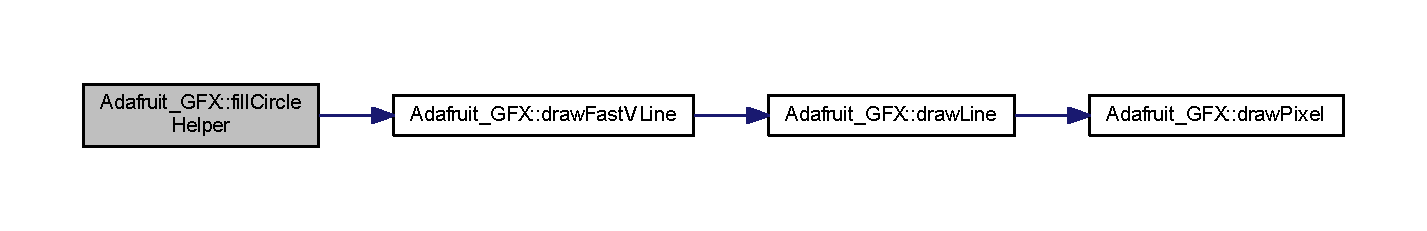
\includegraphics[width=350pt]{d9/d97/class_adafruit___g_f_x_a2242d3560b08c6480084152b6660052a_cgraph}
\end{center}
\end{figure}
Here is the caller graph for this function\+:
\nopagebreak
\begin{figure}[H]
\begin{center}
\leavevmode
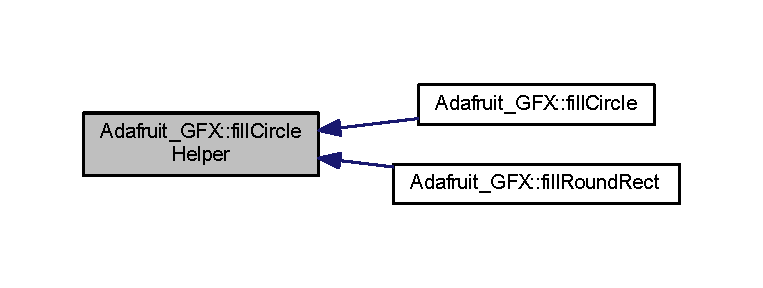
\includegraphics[width=350pt]{d9/d97/class_adafruit___g_f_x_a2242d3560b08c6480084152b6660052a_icgraph}
\end{center}
\end{figure}
\mbox{\Hypertarget{class_adafruit___g_f_x_aa43cf1dfe6c17d040a0f1fd5ffbe9d69}\label{class_adafruit___g_f_x_aa43cf1dfe6c17d040a0f1fd5ffbe9d69}} 
\index{Adafruit\+\_\+\+G\+FX@{Adafruit\+\_\+\+G\+FX}!fill\+Rect@{fill\+Rect}}
\index{fill\+Rect@{fill\+Rect}!Adafruit\+\_\+\+G\+FX@{Adafruit\+\_\+\+G\+FX}}
\subsubsection{\texorpdfstring{fill\+Rect()}{fillRect()}}
{\footnotesize\ttfamily void Adafruit\+\_\+\+G\+F\+X\+::fill\+Rect (\begin{DoxyParamCaption}\item[{int16\+\_\+t}]{x,  }\item[{int16\+\_\+t}]{y,  }\item[{int16\+\_\+t}]{w,  }\item[{int16\+\_\+t}]{h,  }\item[{uint16\+\_\+t}]{color }\end{DoxyParamCaption})}

Here is the call graph for this function\+:
\nopagebreak
\begin{figure}[H]
\begin{center}
\leavevmode
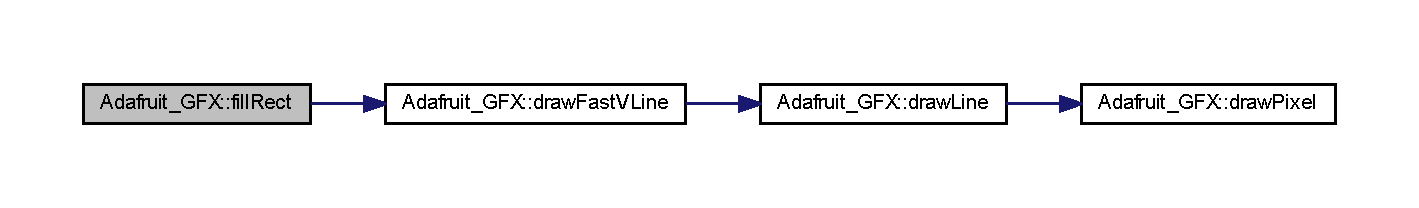
\includegraphics[width=350pt]{d9/d97/class_adafruit___g_f_x_aa43cf1dfe6c17d040a0f1fd5ffbe9d69_cgraph}
\end{center}
\end{figure}
Here is the caller graph for this function\+:
\nopagebreak
\begin{figure}[H]
\begin{center}
\leavevmode
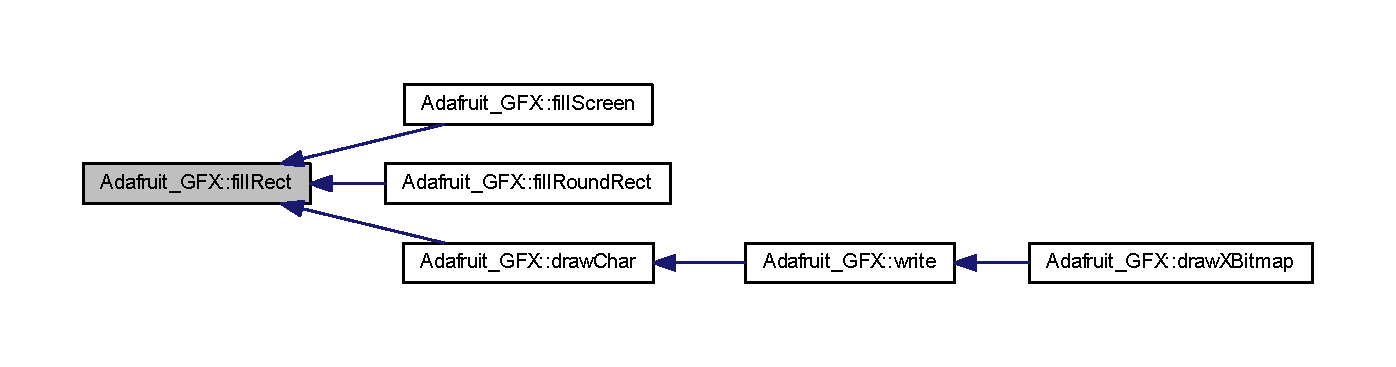
\includegraphics[width=350pt]{d9/d97/class_adafruit___g_f_x_aa43cf1dfe6c17d040a0f1fd5ffbe9d69_icgraph}
\end{center}
\end{figure}
\mbox{\Hypertarget{class_adafruit___g_f_x_a78dc59f6a508bcd3d5ac7af957b8b1ac}\label{class_adafruit___g_f_x_a78dc59f6a508bcd3d5ac7af957b8b1ac}} 
\index{Adafruit\+\_\+\+G\+FX@{Adafruit\+\_\+\+G\+FX}!fill\+Round\+Rect@{fill\+Round\+Rect}}
\index{fill\+Round\+Rect@{fill\+Round\+Rect}!Adafruit\+\_\+\+G\+FX@{Adafruit\+\_\+\+G\+FX}}
\subsubsection{\texorpdfstring{fill\+Round\+Rect()}{fillRoundRect()}}
{\footnotesize\ttfamily void Adafruit\+\_\+\+G\+F\+X\+::fill\+Round\+Rect (\begin{DoxyParamCaption}\item[{int16\+\_\+t}]{x0,  }\item[{int16\+\_\+t}]{y0,  }\item[{int16\+\_\+t}]{w,  }\item[{int16\+\_\+t}]{h,  }\item[{int16\+\_\+t}]{radius,  }\item[{uint16\+\_\+t}]{color }\end{DoxyParamCaption})}

Here is the call graph for this function\+:
\nopagebreak
\begin{figure}[H]
\begin{center}
\leavevmode
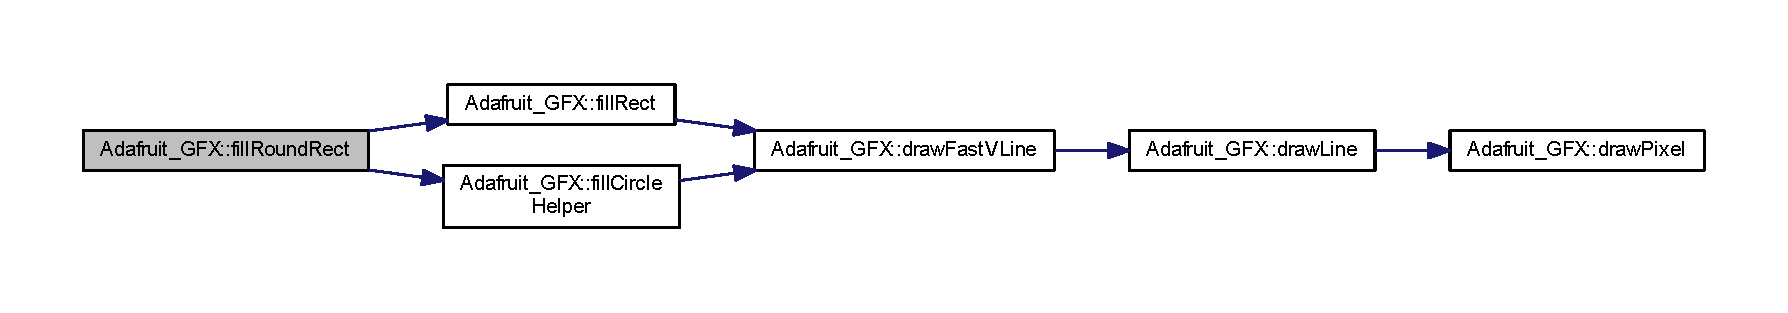
\includegraphics[width=350pt]{d9/d97/class_adafruit___g_f_x_a78dc59f6a508bcd3d5ac7af957b8b1ac_cgraph}
\end{center}
\end{figure}
\mbox{\Hypertarget{class_adafruit___g_f_x_a2b2730aaf2208990928f9c0f85558527}\label{class_adafruit___g_f_x_a2b2730aaf2208990928f9c0f85558527}} 
\index{Adafruit\+\_\+\+G\+FX@{Adafruit\+\_\+\+G\+FX}!fill\+Screen@{fill\+Screen}}
\index{fill\+Screen@{fill\+Screen}!Adafruit\+\_\+\+G\+FX@{Adafruit\+\_\+\+G\+FX}}
\subsubsection{\texorpdfstring{fill\+Screen()}{fillScreen()}}
{\footnotesize\ttfamily void Adafruit\+\_\+\+G\+F\+X\+::fill\+Screen (\begin{DoxyParamCaption}\item[{uint16\+\_\+t}]{color }\end{DoxyParamCaption})}

Here is the call graph for this function\+:
\nopagebreak
\begin{figure}[H]
\begin{center}
\leavevmode
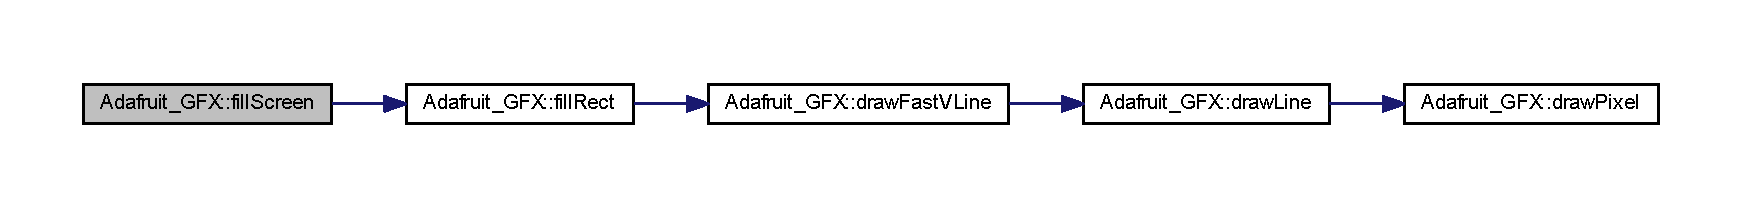
\includegraphics[width=350pt]{d9/d97/class_adafruit___g_f_x_a2b2730aaf2208990928f9c0f85558527_cgraph}
\end{center}
\end{figure}
\mbox{\Hypertarget{class_adafruit___g_f_x_a4cd646a3d9c9d5b3ee50010d0aa387cd}\label{class_adafruit___g_f_x_a4cd646a3d9c9d5b3ee50010d0aa387cd}} 
\index{Adafruit\+\_\+\+G\+FX@{Adafruit\+\_\+\+G\+FX}!fill\+Triangle@{fill\+Triangle}}
\index{fill\+Triangle@{fill\+Triangle}!Adafruit\+\_\+\+G\+FX@{Adafruit\+\_\+\+G\+FX}}
\subsubsection{\texorpdfstring{fill\+Triangle()}{fillTriangle()}}
{\footnotesize\ttfamily void Adafruit\+\_\+\+G\+F\+X\+::fill\+Triangle (\begin{DoxyParamCaption}\item[{int16\+\_\+t}]{x0,  }\item[{int16\+\_\+t}]{y0,  }\item[{int16\+\_\+t}]{x1,  }\item[{int16\+\_\+t}]{y1,  }\item[{int16\+\_\+t}]{x2,  }\item[{int16\+\_\+t}]{y2,  }\item[{uint16\+\_\+t}]{color }\end{DoxyParamCaption})}

Here is the call graph for this function\+:
\nopagebreak
\begin{figure}[H]
\begin{center}
\leavevmode
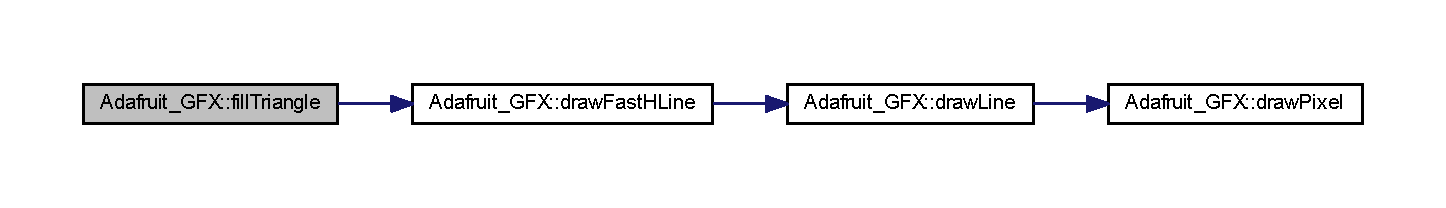
\includegraphics[width=350pt]{d9/d97/class_adafruit___g_f_x_a4cd646a3d9c9d5b3ee50010d0aa387cd_cgraph}
\end{center}
\end{figure}
\mbox{\Hypertarget{class_adafruit___g_f_x_a0d1d15f5f15cad95b4c20f0e9ac9c74b}\label{class_adafruit___g_f_x_a0d1d15f5f15cad95b4c20f0e9ac9c74b}} 
\index{Adafruit\+\_\+\+G\+FX@{Adafruit\+\_\+\+G\+FX}!get\+CursorX@{get\+CursorX}}
\index{get\+CursorX@{get\+CursorX}!Adafruit\+\_\+\+G\+FX@{Adafruit\+\_\+\+G\+FX}}
\subsubsection{\texorpdfstring{get\+Cursor\+X()}{getCursorX()}}
{\footnotesize\ttfamily int16\+\_\+t Adafruit\+\_\+\+G\+F\+X\+::get\+CursorX (\begin{DoxyParamCaption}\item[{void}]{ }\end{DoxyParamCaption}) const}

\mbox{\Hypertarget{class_adafruit___g_f_x_a81c8558cfcb717c4cfbd5475998daed1}\label{class_adafruit___g_f_x_a81c8558cfcb717c4cfbd5475998daed1}} 
\index{Adafruit\+\_\+\+G\+FX@{Adafruit\+\_\+\+G\+FX}!get\+CursorY@{get\+CursorY}}
\index{get\+CursorY@{get\+CursorY}!Adafruit\+\_\+\+G\+FX@{Adafruit\+\_\+\+G\+FX}}
\subsubsection{\texorpdfstring{get\+Cursor\+Y()}{getCursorY()}}
{\footnotesize\ttfamily int16\+\_\+t Adafruit\+\_\+\+G\+F\+X\+::get\+CursorY (\begin{DoxyParamCaption}\item[{void}]{ }\end{DoxyParamCaption}) const}

\mbox{\Hypertarget{class_adafruit___g_f_x_ab90e1378511b93189a7b557d7dda5d73}\label{class_adafruit___g_f_x_ab90e1378511b93189a7b557d7dda5d73}} 
\index{Adafruit\+\_\+\+G\+FX@{Adafruit\+\_\+\+G\+FX}!get\+Rotation@{get\+Rotation}}
\index{get\+Rotation@{get\+Rotation}!Adafruit\+\_\+\+G\+FX@{Adafruit\+\_\+\+G\+FX}}
\subsubsection{\texorpdfstring{get\+Rotation()}{getRotation()}}
{\footnotesize\ttfamily uint8\+\_\+t Adafruit\+\_\+\+G\+F\+X\+::get\+Rotation (\begin{DoxyParamCaption}\item[{void}]{ }\end{DoxyParamCaption}) const}

\mbox{\Hypertarget{class_adafruit___g_f_x_a49da524caa19e5202ed2ed7fd5a3baea}\label{class_adafruit___g_f_x_a49da524caa19e5202ed2ed7fd5a3baea}} 
\index{Adafruit\+\_\+\+G\+FX@{Adafruit\+\_\+\+G\+FX}!height@{height}}
\index{height@{height}!Adafruit\+\_\+\+G\+FX@{Adafruit\+\_\+\+G\+FX}}
\subsubsection{\texorpdfstring{height()}{height()}}
{\footnotesize\ttfamily int16\+\_\+t Adafruit\+\_\+\+G\+F\+X\+::height (\begin{DoxyParamCaption}\item[{void}]{ }\end{DoxyParamCaption}) const}

\mbox{\Hypertarget{class_adafruit___g_f_x_a2fa315803f39a5e73b1841874daf0483}\label{class_adafruit___g_f_x_a2fa315803f39a5e73b1841874daf0483}} 
\index{Adafruit\+\_\+\+G\+FX@{Adafruit\+\_\+\+G\+FX}!invert\+Display@{invert\+Display}}
\index{invert\+Display@{invert\+Display}!Adafruit\+\_\+\+G\+FX@{Adafruit\+\_\+\+G\+FX}}
\subsubsection{\texorpdfstring{invert\+Display()}{invertDisplay()}}
{\footnotesize\ttfamily void Adafruit\+\_\+\+G\+F\+X\+::invert\+Display (\begin{DoxyParamCaption}\item[{boolean}]{i }\end{DoxyParamCaption})}

\mbox{\Hypertarget{class_adafruit___g_f_x_aaf96a40cad0f34dd8ec73494b3866c33}\label{class_adafruit___g_f_x_aaf96a40cad0f34dd8ec73494b3866c33}} 
\index{Adafruit\+\_\+\+G\+FX@{Adafruit\+\_\+\+G\+FX}!set\+Cursor@{set\+Cursor}}
\index{set\+Cursor@{set\+Cursor}!Adafruit\+\_\+\+G\+FX@{Adafruit\+\_\+\+G\+FX}}
\subsubsection{\texorpdfstring{set\+Cursor()}{setCursor()}}
{\footnotesize\ttfamily void Adafruit\+\_\+\+G\+F\+X\+::set\+Cursor (\begin{DoxyParamCaption}\item[{int16\+\_\+t}]{x,  }\item[{int16\+\_\+t}]{y }\end{DoxyParamCaption})}

Here is the caller graph for this function\+:
\nopagebreak
\begin{figure}[H]
\begin{center}
\leavevmode
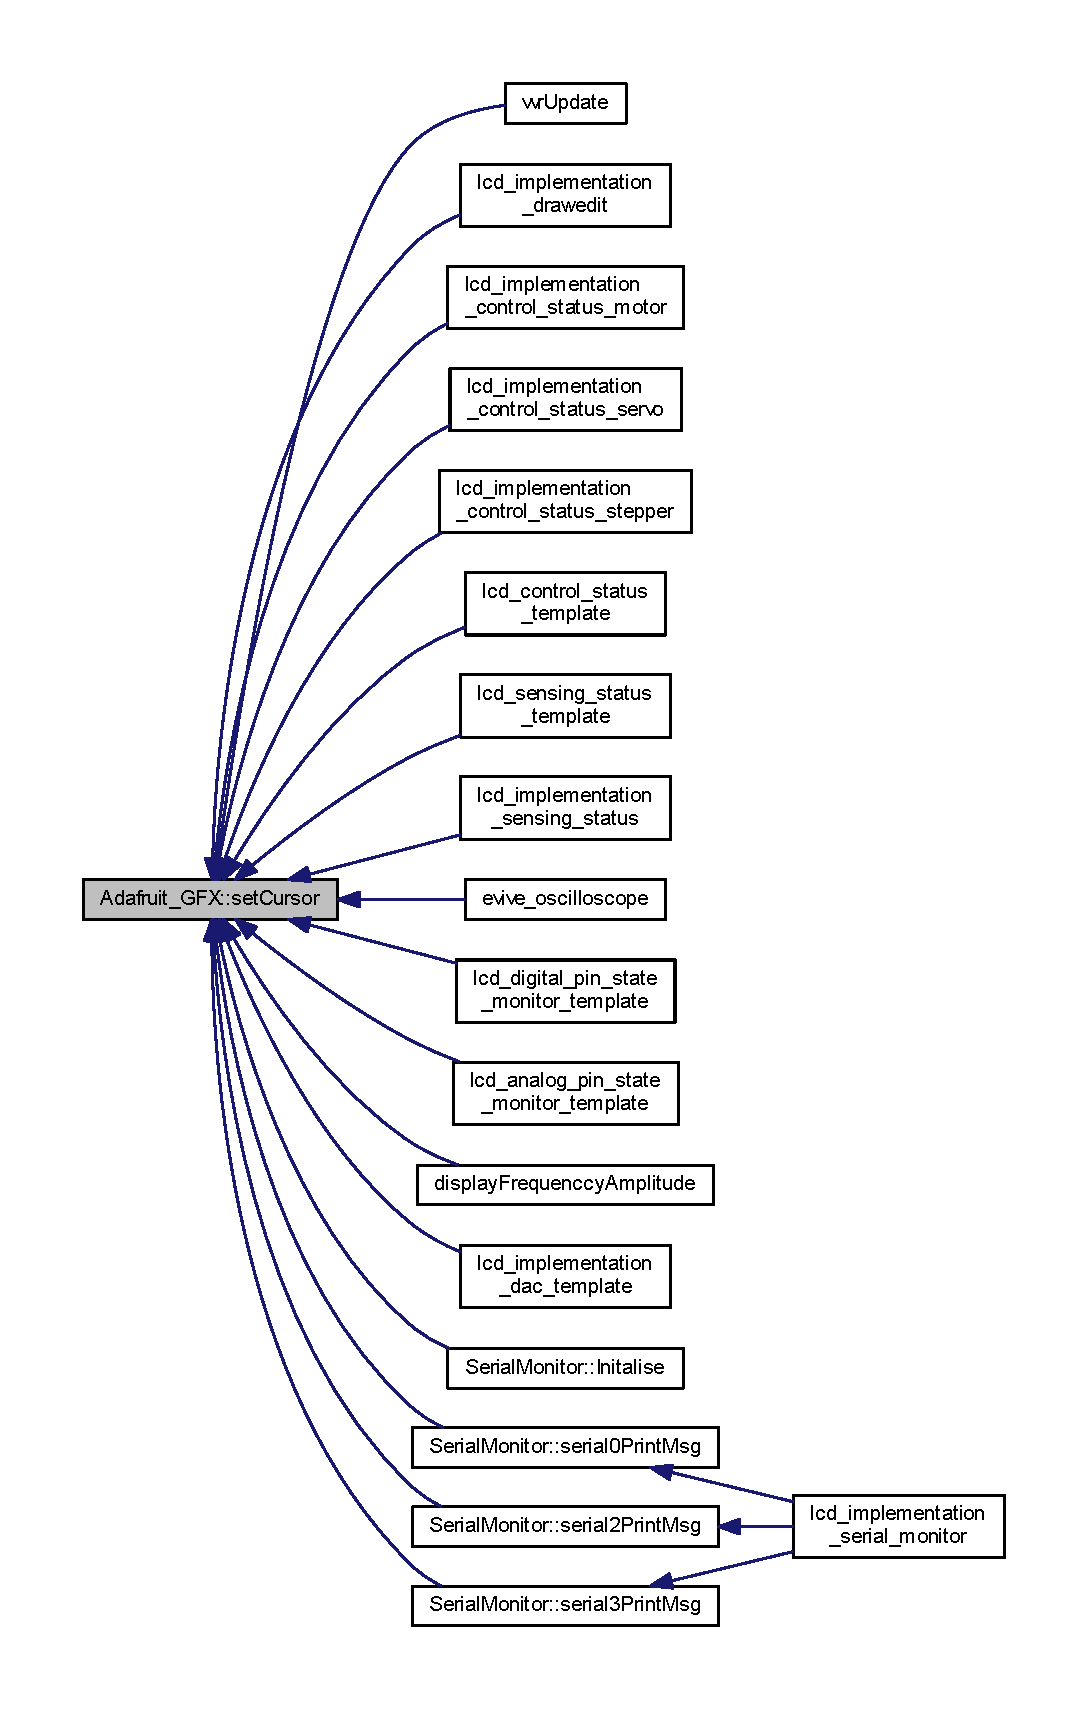
\includegraphics[height=550pt]{d9/d97/class_adafruit___g_f_x_aaf96a40cad0f34dd8ec73494b3866c33_icgraph}
\end{center}
\end{figure}
\mbox{\Hypertarget{class_adafruit___g_f_x_a6ac337c49876cee23ed062a928724675}\label{class_adafruit___g_f_x_a6ac337c49876cee23ed062a928724675}} 
\index{Adafruit\+\_\+\+G\+FX@{Adafruit\+\_\+\+G\+FX}!set\+Rotation@{set\+Rotation}}
\index{set\+Rotation@{set\+Rotation}!Adafruit\+\_\+\+G\+FX@{Adafruit\+\_\+\+G\+FX}}
\subsubsection{\texorpdfstring{set\+Rotation()}{setRotation()}}
{\footnotesize\ttfamily void Adafruit\+\_\+\+G\+F\+X\+::set\+Rotation (\begin{DoxyParamCaption}\item[{uint8\+\_\+t}]{r }\end{DoxyParamCaption})}

\mbox{\Hypertarget{class_adafruit___g_f_x_a59178a0e0c845a14a39b457c43567dd9}\label{class_adafruit___g_f_x_a59178a0e0c845a14a39b457c43567dd9}} 
\index{Adafruit\+\_\+\+G\+FX@{Adafruit\+\_\+\+G\+FX}!set\+Text\+Color@{set\+Text\+Color}}
\index{set\+Text\+Color@{set\+Text\+Color}!Adafruit\+\_\+\+G\+FX@{Adafruit\+\_\+\+G\+FX}}
\subsubsection{\texorpdfstring{set\+Text\+Color()}{setTextColor()}\hspace{0.1cm}{\footnotesize\ttfamily [1/2]}}
{\footnotesize\ttfamily void Adafruit\+\_\+\+G\+F\+X\+::set\+Text\+Color (\begin{DoxyParamCaption}\item[{uint16\+\_\+t}]{c }\end{DoxyParamCaption})}

Here is the caller graph for this function\+:
\nopagebreak
\begin{figure}[H]
\begin{center}
\leavevmode
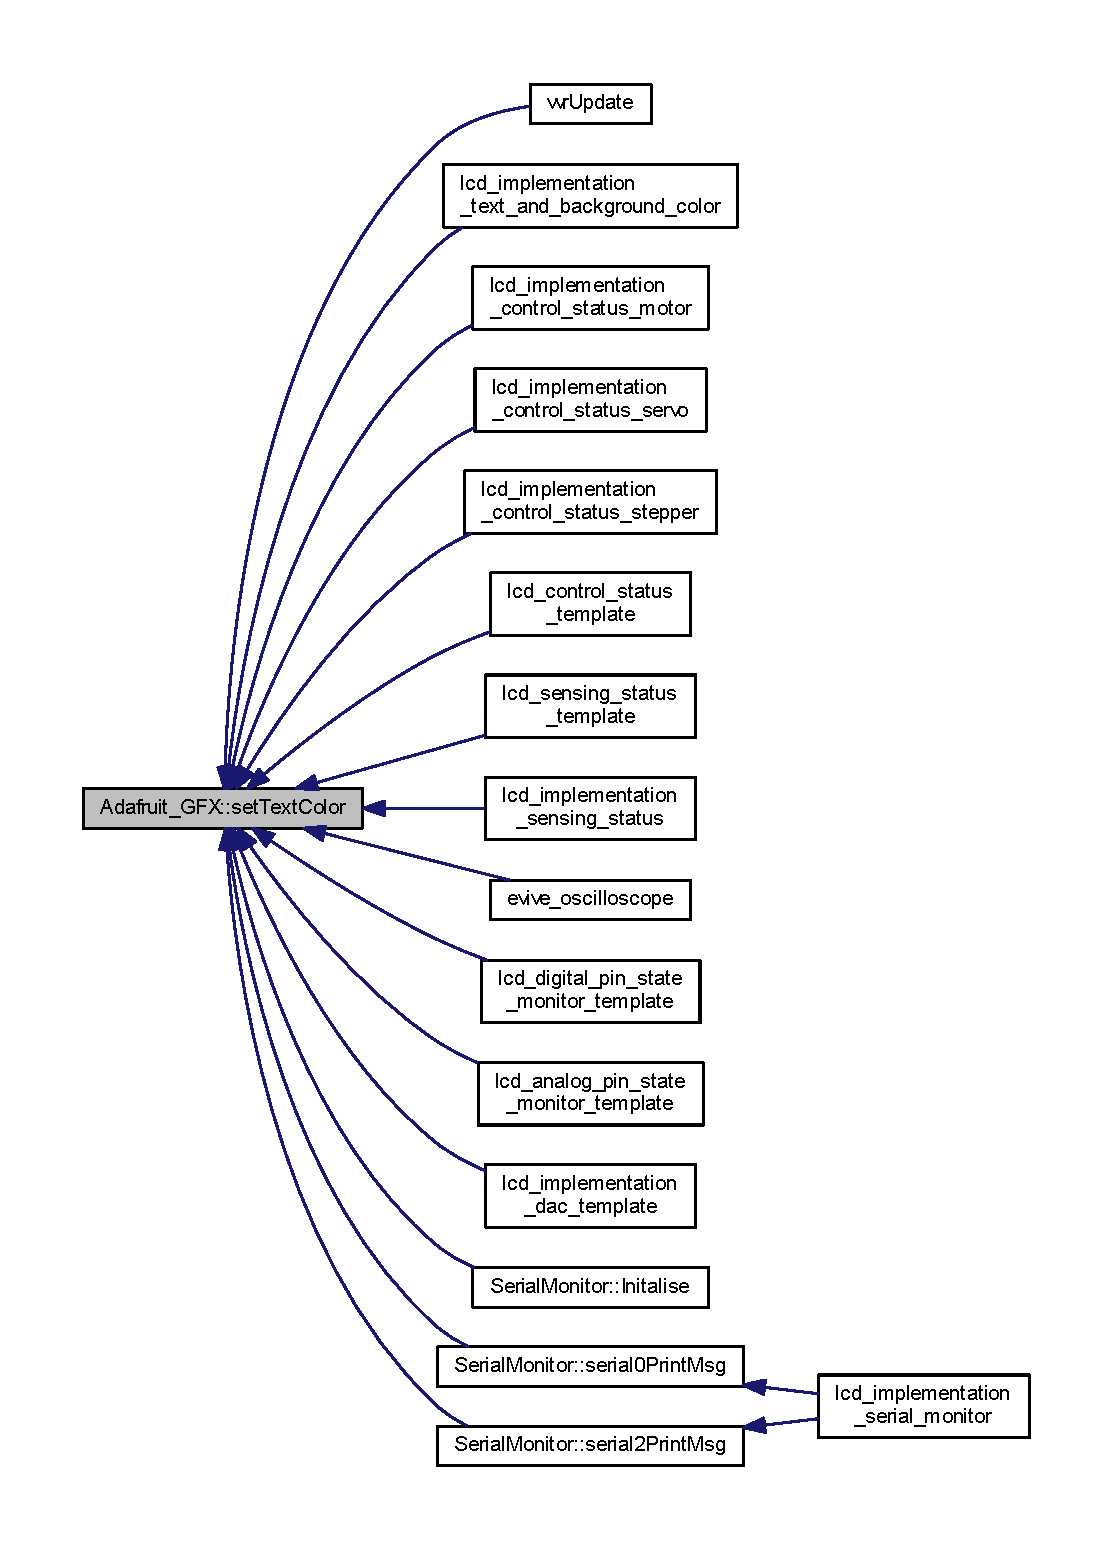
\includegraphics[width=350pt]{d9/d97/class_adafruit___g_f_x_a59178a0e0c845a14a39b457c43567dd9_icgraph}
\end{center}
\end{figure}
\mbox{\Hypertarget{class_adafruit___g_f_x_ab6e88c585d3ab6b4f95199361f224fc6}\label{class_adafruit___g_f_x_ab6e88c585d3ab6b4f95199361f224fc6}} 
\index{Adafruit\+\_\+\+G\+FX@{Adafruit\+\_\+\+G\+FX}!set\+Text\+Color@{set\+Text\+Color}}
\index{set\+Text\+Color@{set\+Text\+Color}!Adafruit\+\_\+\+G\+FX@{Adafruit\+\_\+\+G\+FX}}
\subsubsection{\texorpdfstring{set\+Text\+Color()}{setTextColor()}\hspace{0.1cm}{\footnotesize\ttfamily [2/2]}}
{\footnotesize\ttfamily void Adafruit\+\_\+\+G\+F\+X\+::set\+Text\+Color (\begin{DoxyParamCaption}\item[{uint16\+\_\+t}]{c,  }\item[{uint16\+\_\+t}]{bg }\end{DoxyParamCaption})}

\mbox{\Hypertarget{class_adafruit___g_f_x_a39eb4a8a2c9fa4ab7d58ceffd19535d5}\label{class_adafruit___g_f_x_a39eb4a8a2c9fa4ab7d58ceffd19535d5}} 
\index{Adafruit\+\_\+\+G\+FX@{Adafruit\+\_\+\+G\+FX}!set\+Text\+Size@{set\+Text\+Size}}
\index{set\+Text\+Size@{set\+Text\+Size}!Adafruit\+\_\+\+G\+FX@{Adafruit\+\_\+\+G\+FX}}
\subsubsection{\texorpdfstring{set\+Text\+Size()}{setTextSize()}}
{\footnotesize\ttfamily void Adafruit\+\_\+\+G\+F\+X\+::set\+Text\+Size (\begin{DoxyParamCaption}\item[{uint8\+\_\+t}]{s }\end{DoxyParamCaption})}

Here is the caller graph for this function\+:
\nopagebreak
\begin{figure}[H]
\begin{center}
\leavevmode
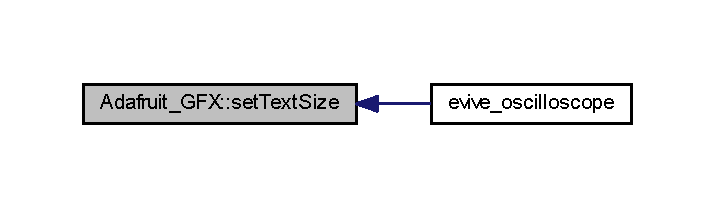
\includegraphics[width=343pt]{d9/d97/class_adafruit___g_f_x_a39eb4a8a2c9fa4ab7d58ceffd19535d5_icgraph}
\end{center}
\end{figure}
\mbox{\Hypertarget{class_adafruit___g_f_x_aeeacd62bf26f3e7abbdc4b5b50faa6fa}\label{class_adafruit___g_f_x_aeeacd62bf26f3e7abbdc4b5b50faa6fa}} 
\index{Adafruit\+\_\+\+G\+FX@{Adafruit\+\_\+\+G\+FX}!set\+Text\+Wrap@{set\+Text\+Wrap}}
\index{set\+Text\+Wrap@{set\+Text\+Wrap}!Adafruit\+\_\+\+G\+FX@{Adafruit\+\_\+\+G\+FX}}
\subsubsection{\texorpdfstring{set\+Text\+Wrap()}{setTextWrap()}}
{\footnotesize\ttfamily void Adafruit\+\_\+\+G\+F\+X\+::set\+Text\+Wrap (\begin{DoxyParamCaption}\item[{boolean}]{w }\end{DoxyParamCaption})}

Here is the caller graph for this function\+:
\nopagebreak
\begin{figure}[H]
\begin{center}
\leavevmode
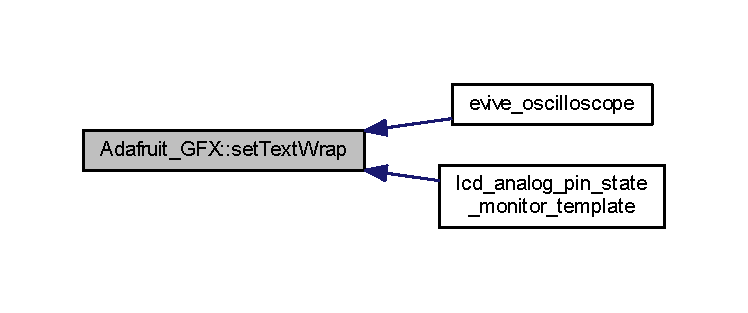
\includegraphics[width=350pt]{d9/d97/class_adafruit___g_f_x_aeeacd62bf26f3e7abbdc4b5b50faa6fa_icgraph}
\end{center}
\end{figure}
\mbox{\Hypertarget{class_adafruit___g_f_x_a324b5361e7198ef0e79eaf4c80bddfc7}\label{class_adafruit___g_f_x_a324b5361e7198ef0e79eaf4c80bddfc7}} 
\index{Adafruit\+\_\+\+G\+FX@{Adafruit\+\_\+\+G\+FX}!width@{width}}
\index{width@{width}!Adafruit\+\_\+\+G\+FX@{Adafruit\+\_\+\+G\+FX}}
\subsubsection{\texorpdfstring{width()}{width()}}
{\footnotesize\ttfamily int16\+\_\+t Adafruit\+\_\+\+G\+F\+X\+::width (\begin{DoxyParamCaption}\item[{void}]{ }\end{DoxyParamCaption}) const}

\mbox{\Hypertarget{class_adafruit___g_f_x_af4978ea0cf0c0b0540567e82d8fa9900}\label{class_adafruit___g_f_x_af4978ea0cf0c0b0540567e82d8fa9900}} 
\index{Adafruit\+\_\+\+G\+FX@{Adafruit\+\_\+\+G\+FX}!write@{write}}
\index{write@{write}!Adafruit\+\_\+\+G\+FX@{Adafruit\+\_\+\+G\+FX}}
\subsubsection{\texorpdfstring{write()}{write()}}
{\footnotesize\ttfamily void Adafruit\+\_\+\+G\+F\+X\+::write (\begin{DoxyParamCaption}\item[{uint8\+\_\+t}]{c }\end{DoxyParamCaption})\hspace{0.3cm}{\ttfamily [virtual]}}

Here is the call graph for this function\+:
\nopagebreak
\begin{figure}[H]
\begin{center}
\leavevmode
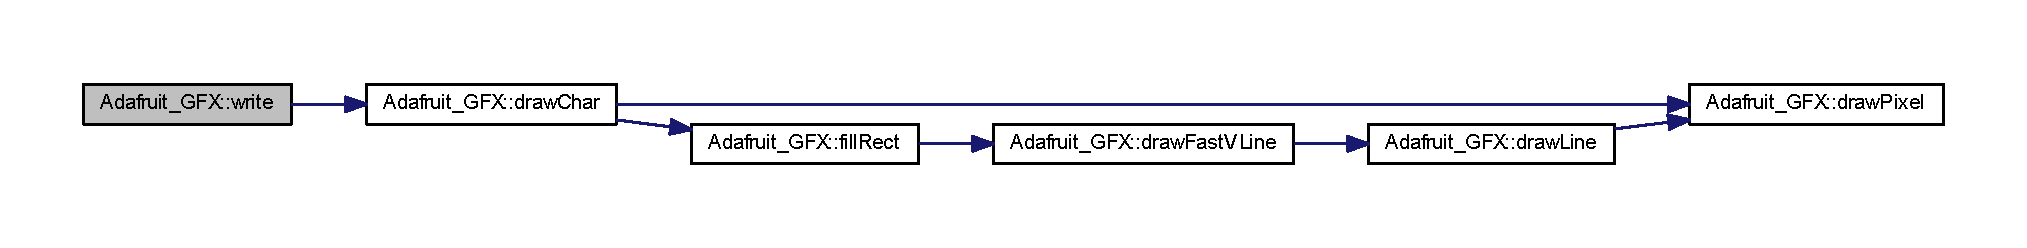
\includegraphics[width=350pt]{d9/d97/class_adafruit___g_f_x_af4978ea0cf0c0b0540567e82d8fa9900_cgraph}
\end{center}
\end{figure}
Here is the caller graph for this function\+:
\nopagebreak
\begin{figure}[H]
\begin{center}
\leavevmode
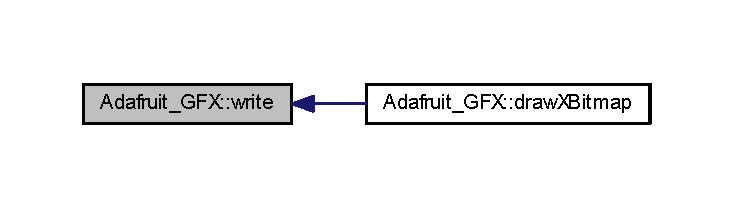
\includegraphics[width=350pt]{d9/d97/class_adafruit___g_f_x_af4978ea0cf0c0b0540567e82d8fa9900_icgraph}
\end{center}
\end{figure}


\subsection{Member Data Documentation}
\mbox{\Hypertarget{class_adafruit___g_f_x_aaef3d4d239641084cd3825a8b1042e01}\label{class_adafruit___g_f_x_aaef3d4d239641084cd3825a8b1042e01}} 
\index{Adafruit\+\_\+\+G\+FX@{Adafruit\+\_\+\+G\+FX}!\+\_\+cp437@{\+\_\+cp437}}
\index{\+\_\+cp437@{\+\_\+cp437}!Adafruit\+\_\+\+G\+FX@{Adafruit\+\_\+\+G\+FX}}
\subsubsection{\texorpdfstring{\+\_\+cp437}{\_cp437}}
{\footnotesize\ttfamily boolean Adafruit\+\_\+\+G\+F\+X\+::\+\_\+cp437\hspace{0.3cm}{\ttfamily [protected]}}

\mbox{\Hypertarget{class_adafruit___g_f_x_ab9bb0cbc2455f64dce2a5ec36307aa94}\label{class_adafruit___g_f_x_ab9bb0cbc2455f64dce2a5ec36307aa94}} 
\index{Adafruit\+\_\+\+G\+FX@{Adafruit\+\_\+\+G\+FX}!\+\_\+height@{\+\_\+height}}
\index{\+\_\+height@{\+\_\+height}!Adafruit\+\_\+\+G\+FX@{Adafruit\+\_\+\+G\+FX}}
\subsubsection{\texorpdfstring{\+\_\+height}{\_height}}
{\footnotesize\ttfamily int16\+\_\+t Adafruit\+\_\+\+G\+F\+X\+::\+\_\+height\hspace{0.3cm}{\ttfamily [protected]}}

\mbox{\Hypertarget{class_adafruit___g_f_x_ab237f850a033492f5e745d79405a097a}\label{class_adafruit___g_f_x_ab237f850a033492f5e745d79405a097a}} 
\index{Adafruit\+\_\+\+G\+FX@{Adafruit\+\_\+\+G\+FX}!\+\_\+width@{\+\_\+width}}
\index{\+\_\+width@{\+\_\+width}!Adafruit\+\_\+\+G\+FX@{Adafruit\+\_\+\+G\+FX}}
\subsubsection{\texorpdfstring{\+\_\+width}{\_width}}
{\footnotesize\ttfamily int16\+\_\+t Adafruit\+\_\+\+G\+F\+X\+::\+\_\+width\hspace{0.3cm}{\ttfamily [protected]}}

\mbox{\Hypertarget{class_adafruit___g_f_x_a8f8983cea8d81a7c8e9d05eef36318e2}\label{class_adafruit___g_f_x_a8f8983cea8d81a7c8e9d05eef36318e2}} 
\index{Adafruit\+\_\+\+G\+FX@{Adafruit\+\_\+\+G\+FX}!cursor\+\_\+x@{cursor\+\_\+x}}
\index{cursor\+\_\+x@{cursor\+\_\+x}!Adafruit\+\_\+\+G\+FX@{Adafruit\+\_\+\+G\+FX}}
\subsubsection{\texorpdfstring{cursor\+\_\+x}{cursor\_x}}
{\footnotesize\ttfamily int16\+\_\+t Adafruit\+\_\+\+G\+F\+X\+::cursor\+\_\+x\hspace{0.3cm}{\ttfamily [protected]}}

\mbox{\Hypertarget{class_adafruit___g_f_x_aebe0a38f6e6fd59cb81620c4696286c9}\label{class_adafruit___g_f_x_aebe0a38f6e6fd59cb81620c4696286c9}} 
\index{Adafruit\+\_\+\+G\+FX@{Adafruit\+\_\+\+G\+FX}!cursor\+\_\+y@{cursor\+\_\+y}}
\index{cursor\+\_\+y@{cursor\+\_\+y}!Adafruit\+\_\+\+G\+FX@{Adafruit\+\_\+\+G\+FX}}
\subsubsection{\texorpdfstring{cursor\+\_\+y}{cursor\_y}}
{\footnotesize\ttfamily int16\+\_\+t Adafruit\+\_\+\+G\+F\+X\+::cursor\+\_\+y\hspace{0.3cm}{\ttfamily [protected]}}

\mbox{\Hypertarget{class_adafruit___g_f_x_a6b3665babcb73df381563016e9f71bdb}\label{class_adafruit___g_f_x_a6b3665babcb73df381563016e9f71bdb}} 
\index{Adafruit\+\_\+\+G\+FX@{Adafruit\+\_\+\+G\+FX}!H\+E\+I\+G\+HT@{H\+E\+I\+G\+HT}}
\index{H\+E\+I\+G\+HT@{H\+E\+I\+G\+HT}!Adafruit\+\_\+\+G\+FX@{Adafruit\+\_\+\+G\+FX}}
\subsubsection{\texorpdfstring{H\+E\+I\+G\+HT}{HEIGHT}}
{\footnotesize\ttfamily const int16\+\_\+t Adafruit\+\_\+\+G\+F\+X\+::\+H\+E\+I\+G\+HT\hspace{0.3cm}{\ttfamily [protected]}}

\mbox{\Hypertarget{class_adafruit___g_f_x_a37a479d28fb11906ce516e983b1af926}\label{class_adafruit___g_f_x_a37a479d28fb11906ce516e983b1af926}} 
\index{Adafruit\+\_\+\+G\+FX@{Adafruit\+\_\+\+G\+FX}!rotation@{rotation}}
\index{rotation@{rotation}!Adafruit\+\_\+\+G\+FX@{Adafruit\+\_\+\+G\+FX}}
\subsubsection{\texorpdfstring{rotation}{rotation}}
{\footnotesize\ttfamily uint8\+\_\+t Adafruit\+\_\+\+G\+F\+X\+::rotation\hspace{0.3cm}{\ttfamily [protected]}}

\mbox{\Hypertarget{class_adafruit___g_f_x_a23e7a4efcab0b1588dc0cafa14b1fac1}\label{class_adafruit___g_f_x_a23e7a4efcab0b1588dc0cafa14b1fac1}} 
\index{Adafruit\+\_\+\+G\+FX@{Adafruit\+\_\+\+G\+FX}!textbgcolor@{textbgcolor}}
\index{textbgcolor@{textbgcolor}!Adafruit\+\_\+\+G\+FX@{Adafruit\+\_\+\+G\+FX}}
\subsubsection{\texorpdfstring{textbgcolor}{textbgcolor}}
{\footnotesize\ttfamily uint16\+\_\+t Adafruit\+\_\+\+G\+F\+X\+::textbgcolor\hspace{0.3cm}{\ttfamily [protected]}}

\mbox{\Hypertarget{class_adafruit___g_f_x_a8c6d23a386651136fd9530a5b7046591}\label{class_adafruit___g_f_x_a8c6d23a386651136fd9530a5b7046591}} 
\index{Adafruit\+\_\+\+G\+FX@{Adafruit\+\_\+\+G\+FX}!textcolor@{textcolor}}
\index{textcolor@{textcolor}!Adafruit\+\_\+\+G\+FX@{Adafruit\+\_\+\+G\+FX}}
\subsubsection{\texorpdfstring{textcolor}{textcolor}}
{\footnotesize\ttfamily uint16\+\_\+t Adafruit\+\_\+\+G\+F\+X\+::textcolor\hspace{0.3cm}{\ttfamily [protected]}}

\mbox{\Hypertarget{class_adafruit___g_f_x_ac293848b8fe8c46107d1a491f6a5168d}\label{class_adafruit___g_f_x_ac293848b8fe8c46107d1a491f6a5168d}} 
\index{Adafruit\+\_\+\+G\+FX@{Adafruit\+\_\+\+G\+FX}!textsize@{textsize}}
\index{textsize@{textsize}!Adafruit\+\_\+\+G\+FX@{Adafruit\+\_\+\+G\+FX}}
\subsubsection{\texorpdfstring{textsize}{textsize}}
{\footnotesize\ttfamily uint8\+\_\+t Adafruit\+\_\+\+G\+F\+X\+::textsize\hspace{0.3cm}{\ttfamily [protected]}}

\mbox{\Hypertarget{class_adafruit___g_f_x_ab693a8ac5d94c50c2558b5a3795ddde4}\label{class_adafruit___g_f_x_ab693a8ac5d94c50c2558b5a3795ddde4}} 
\index{Adafruit\+\_\+\+G\+FX@{Adafruit\+\_\+\+G\+FX}!W\+I\+D\+TH@{W\+I\+D\+TH}}
\index{W\+I\+D\+TH@{W\+I\+D\+TH}!Adafruit\+\_\+\+G\+FX@{Adafruit\+\_\+\+G\+FX}}
\subsubsection{\texorpdfstring{W\+I\+D\+TH}{WIDTH}}
{\footnotesize\ttfamily const int16\+\_\+t Adafruit\+\_\+\+G\+F\+X\+::\+W\+I\+D\+TH\hspace{0.3cm}{\ttfamily [protected]}}

\mbox{\Hypertarget{class_adafruit___g_f_x_ad6bd603e01861212829d536312a7190b}\label{class_adafruit___g_f_x_ad6bd603e01861212829d536312a7190b}} 
\index{Adafruit\+\_\+\+G\+FX@{Adafruit\+\_\+\+G\+FX}!wrap@{wrap}}
\index{wrap@{wrap}!Adafruit\+\_\+\+G\+FX@{Adafruit\+\_\+\+G\+FX}}
\subsubsection{\texorpdfstring{wrap}{wrap}}
{\footnotesize\ttfamily boolean Adafruit\+\_\+\+G\+F\+X\+::wrap\hspace{0.3cm}{\ttfamily [protected]}}



The documentation for this class was generated from the following files\+:\begin{DoxyCompactItemize}
\item 
\hyperlink{_adafruit___g_f_x_8h}{Adafruit\+\_\+\+G\+F\+X.\+h}\item 
\hyperlink{_adafruit___g_f_x_8cpp}{Adafruit\+\_\+\+G\+F\+X.\+cpp}\end{DoxyCompactItemize}

\hypertarget{class_adafruit___g_f_x___button}{}\section{Adafruit\+\_\+\+G\+F\+X\+\_\+\+Button Class Reference}
\label{class_adafruit___g_f_x___button}\index{Adafruit\+\_\+\+G\+F\+X\+\_\+\+Button@{Adafruit\+\_\+\+G\+F\+X\+\_\+\+Button}}


{\ttfamily \#include $<$Adafruit\+\_\+\+G\+F\+X.\+h$>$}



Collaboration diagram for Adafruit\+\_\+\+G\+F\+X\+\_\+\+Button\+:
\nopagebreak
\begin{figure}[H]
\begin{center}
\leavevmode
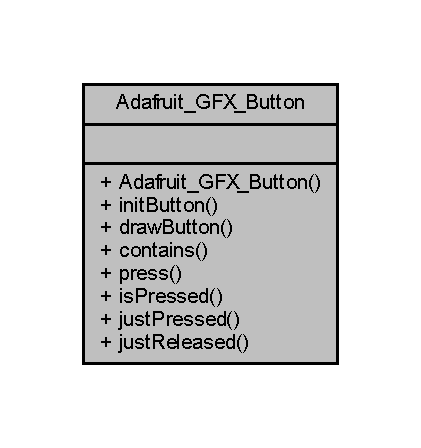
\includegraphics[width=202pt]{d9/dc7/class_adafruit___g_f_x___button__coll__graph}
\end{center}
\end{figure}
\subsection*{Public Member Functions}
\begin{DoxyCompactItemize}
\item 
\hyperlink{class_adafruit___g_f_x___button_a2232fef797e2d21f931eeda59d790d09}{Adafruit\+\_\+\+G\+F\+X\+\_\+\+Button} (void)
\item 
void \hyperlink{class_adafruit___g_f_x___button_a9c5cb82000fcba9b660a86e08a669e07}{init\+Button} (\hyperlink{class_adafruit___g_f_x}{Adafruit\+\_\+\+G\+FX} $\ast$gfx, int16\+\_\+t x, int16\+\_\+t y, uint8\+\_\+t w, uint8\+\_\+t h, uint16\+\_\+t outline, uint16\+\_\+t fill, uint16\+\_\+t textcolor, char $\ast$label, uint8\+\_\+t textsize)
\item 
void \hyperlink{class_adafruit___g_f_x___button_a1d9329970f085c5111e239be90005371}{draw\+Button} (boolean inverted=false)
\item 
boolean \hyperlink{class_adafruit___g_f_x___button_aa5fb594cf6f9cd4c1815a7c1011b5830}{contains} (int16\+\_\+t x, int16\+\_\+t y)
\item 
void \hyperlink{class_adafruit___g_f_x___button_a221d9753f7d8e8f7f9c1ebbee69d02bd}{press} (boolean p)
\item 
boolean \hyperlink{class_adafruit___g_f_x___button_a1faefaf249e868786a416bc097e2cf07}{is\+Pressed} ()
\item 
boolean \hyperlink{class_adafruit___g_f_x___button_a41bcfc81edaf30a11d171a69e7e7c679}{just\+Pressed} ()
\item 
boolean \hyperlink{class_adafruit___g_f_x___button_a8a139332b95997168ba0da37973d2887}{just\+Released} ()
\end{DoxyCompactItemize}


\subsection{Constructor \& Destructor Documentation}
\mbox{\Hypertarget{class_adafruit___g_f_x___button_a2232fef797e2d21f931eeda59d790d09}\label{class_adafruit___g_f_x___button_a2232fef797e2d21f931eeda59d790d09}} 
\index{Adafruit\+\_\+\+G\+F\+X\+\_\+\+Button@{Adafruit\+\_\+\+G\+F\+X\+\_\+\+Button}!Adafruit\+\_\+\+G\+F\+X\+\_\+\+Button@{Adafruit\+\_\+\+G\+F\+X\+\_\+\+Button}}
\index{Adafruit\+\_\+\+G\+F\+X\+\_\+\+Button@{Adafruit\+\_\+\+G\+F\+X\+\_\+\+Button}!Adafruit\+\_\+\+G\+F\+X\+\_\+\+Button@{Adafruit\+\_\+\+G\+F\+X\+\_\+\+Button}}
\subsubsection{\texorpdfstring{Adafruit\+\_\+\+G\+F\+X\+\_\+\+Button()}{Adafruit\_GFX\_Button()}}
{\footnotesize\ttfamily Adafruit\+\_\+\+G\+F\+X\+\_\+\+Button\+::\+Adafruit\+\_\+\+G\+F\+X\+\_\+\+Button (\begin{DoxyParamCaption}\item[{void}]{ }\end{DoxyParamCaption})}



\subsection{Member Function Documentation}
\mbox{\Hypertarget{class_adafruit___g_f_x___button_aa5fb594cf6f9cd4c1815a7c1011b5830}\label{class_adafruit___g_f_x___button_aa5fb594cf6f9cd4c1815a7c1011b5830}} 
\index{Adafruit\+\_\+\+G\+F\+X\+\_\+\+Button@{Adafruit\+\_\+\+G\+F\+X\+\_\+\+Button}!contains@{contains}}
\index{contains@{contains}!Adafruit\+\_\+\+G\+F\+X\+\_\+\+Button@{Adafruit\+\_\+\+G\+F\+X\+\_\+\+Button}}
\subsubsection{\texorpdfstring{contains()}{contains()}}
{\footnotesize\ttfamily boolean Adafruit\+\_\+\+G\+F\+X\+\_\+\+Button\+::contains (\begin{DoxyParamCaption}\item[{int16\+\_\+t}]{x,  }\item[{int16\+\_\+t}]{y }\end{DoxyParamCaption})}

\mbox{\Hypertarget{class_adafruit___g_f_x___button_a1d9329970f085c5111e239be90005371}\label{class_adafruit___g_f_x___button_a1d9329970f085c5111e239be90005371}} 
\index{Adafruit\+\_\+\+G\+F\+X\+\_\+\+Button@{Adafruit\+\_\+\+G\+F\+X\+\_\+\+Button}!draw\+Button@{draw\+Button}}
\index{draw\+Button@{draw\+Button}!Adafruit\+\_\+\+G\+F\+X\+\_\+\+Button@{Adafruit\+\_\+\+G\+F\+X\+\_\+\+Button}}
\subsubsection{\texorpdfstring{draw\+Button()}{drawButton()}}
{\footnotesize\ttfamily void Adafruit\+\_\+\+G\+F\+X\+\_\+\+Button\+::draw\+Button (\begin{DoxyParamCaption}\item[{boolean}]{inverted = {\ttfamily false} }\end{DoxyParamCaption})}

\mbox{\Hypertarget{class_adafruit___g_f_x___button_a9c5cb82000fcba9b660a86e08a669e07}\label{class_adafruit___g_f_x___button_a9c5cb82000fcba9b660a86e08a669e07}} 
\index{Adafruit\+\_\+\+G\+F\+X\+\_\+\+Button@{Adafruit\+\_\+\+G\+F\+X\+\_\+\+Button}!init\+Button@{init\+Button}}
\index{init\+Button@{init\+Button}!Adafruit\+\_\+\+G\+F\+X\+\_\+\+Button@{Adafruit\+\_\+\+G\+F\+X\+\_\+\+Button}}
\subsubsection{\texorpdfstring{init\+Button()}{initButton()}}
{\footnotesize\ttfamily void Adafruit\+\_\+\+G\+F\+X\+\_\+\+Button\+::init\+Button (\begin{DoxyParamCaption}\item[{\hyperlink{class_adafruit___g_f_x}{Adafruit\+\_\+\+G\+FX} $\ast$}]{gfx,  }\item[{int16\+\_\+t}]{x,  }\item[{int16\+\_\+t}]{y,  }\item[{uint8\+\_\+t}]{w,  }\item[{uint8\+\_\+t}]{h,  }\item[{uint16\+\_\+t}]{outline,  }\item[{uint16\+\_\+t}]{fill,  }\item[{uint16\+\_\+t}]{textcolor,  }\item[{char $\ast$}]{label,  }\item[{uint8\+\_\+t}]{textsize }\end{DoxyParamCaption})}

\mbox{\Hypertarget{class_adafruit___g_f_x___button_a1faefaf249e868786a416bc097e2cf07}\label{class_adafruit___g_f_x___button_a1faefaf249e868786a416bc097e2cf07}} 
\index{Adafruit\+\_\+\+G\+F\+X\+\_\+\+Button@{Adafruit\+\_\+\+G\+F\+X\+\_\+\+Button}!is\+Pressed@{is\+Pressed}}
\index{is\+Pressed@{is\+Pressed}!Adafruit\+\_\+\+G\+F\+X\+\_\+\+Button@{Adafruit\+\_\+\+G\+F\+X\+\_\+\+Button}}
\subsubsection{\texorpdfstring{is\+Pressed()}{isPressed()}}
{\footnotesize\ttfamily boolean Adafruit\+\_\+\+G\+F\+X\+\_\+\+Button\+::is\+Pressed (\begin{DoxyParamCaption}{ }\end{DoxyParamCaption})}

\mbox{\Hypertarget{class_adafruit___g_f_x___button_a41bcfc81edaf30a11d171a69e7e7c679}\label{class_adafruit___g_f_x___button_a41bcfc81edaf30a11d171a69e7e7c679}} 
\index{Adafruit\+\_\+\+G\+F\+X\+\_\+\+Button@{Adafruit\+\_\+\+G\+F\+X\+\_\+\+Button}!just\+Pressed@{just\+Pressed}}
\index{just\+Pressed@{just\+Pressed}!Adafruit\+\_\+\+G\+F\+X\+\_\+\+Button@{Adafruit\+\_\+\+G\+F\+X\+\_\+\+Button}}
\subsubsection{\texorpdfstring{just\+Pressed()}{justPressed()}}
{\footnotesize\ttfamily boolean Adafruit\+\_\+\+G\+F\+X\+\_\+\+Button\+::just\+Pressed (\begin{DoxyParamCaption}{ }\end{DoxyParamCaption})}

\mbox{\Hypertarget{class_adafruit___g_f_x___button_a8a139332b95997168ba0da37973d2887}\label{class_adafruit___g_f_x___button_a8a139332b95997168ba0da37973d2887}} 
\index{Adafruit\+\_\+\+G\+F\+X\+\_\+\+Button@{Adafruit\+\_\+\+G\+F\+X\+\_\+\+Button}!just\+Released@{just\+Released}}
\index{just\+Released@{just\+Released}!Adafruit\+\_\+\+G\+F\+X\+\_\+\+Button@{Adafruit\+\_\+\+G\+F\+X\+\_\+\+Button}}
\subsubsection{\texorpdfstring{just\+Released()}{justReleased()}}
{\footnotesize\ttfamily boolean Adafruit\+\_\+\+G\+F\+X\+\_\+\+Button\+::just\+Released (\begin{DoxyParamCaption}{ }\end{DoxyParamCaption})}

\mbox{\Hypertarget{class_adafruit___g_f_x___button_a221d9753f7d8e8f7f9c1ebbee69d02bd}\label{class_adafruit___g_f_x___button_a221d9753f7d8e8f7f9c1ebbee69d02bd}} 
\index{Adafruit\+\_\+\+G\+F\+X\+\_\+\+Button@{Adafruit\+\_\+\+G\+F\+X\+\_\+\+Button}!press@{press}}
\index{press@{press}!Adafruit\+\_\+\+G\+F\+X\+\_\+\+Button@{Adafruit\+\_\+\+G\+F\+X\+\_\+\+Button}}
\subsubsection{\texorpdfstring{press()}{press()}}
{\footnotesize\ttfamily void Adafruit\+\_\+\+G\+F\+X\+\_\+\+Button\+::press (\begin{DoxyParamCaption}\item[{boolean}]{p }\end{DoxyParamCaption})}



The documentation for this class was generated from the following files\+:\begin{DoxyCompactItemize}
\item 
\hyperlink{_adafruit___g_f_x_8h}{Adafruit\+\_\+\+G\+F\+X.\+h}\item 
\hyperlink{_adafruit___g_f_x_8cpp}{Adafruit\+\_\+\+G\+F\+X.\+cpp}\end{DoxyCompactItemize}

\hypertarget{class_adafruit___m_p_r121}{}\section{Adafruit\+\_\+\+M\+P\+R121 Class Reference}
\label{class_adafruit___m_p_r121}\index{Adafruit\+\_\+\+M\+P\+R121@{Adafruit\+\_\+\+M\+P\+R121}}


{\ttfamily \#include $<$Adafruit\+\_\+\+M\+P\+R121.\+h$>$}



Collaboration diagram for Adafruit\+\_\+\+M\+P\+R121\+:
\nopagebreak
\begin{figure}[H]
\begin{center}
\leavevmode
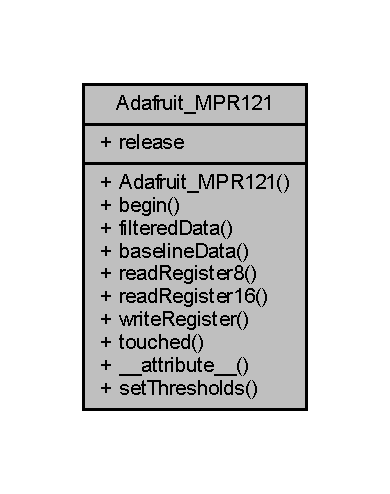
\includegraphics[width=187pt]{d3/d64/class_adafruit___m_p_r121__coll__graph}
\end{center}
\end{figure}
\subsection*{Public Member Functions}
\begin{DoxyCompactItemize}
\item 
\hyperlink{class_adafruit___m_p_r121_a41a5019501062ae1f94c121c580514b5}{Adafruit\+\_\+\+M\+P\+R121} (void)
\item 
boolean \hyperlink{class_adafruit___m_p_r121_ae269064c42ced60c7450eab53ada5eee}{begin} (uint8\+\_\+t i2caddr=\hyperlink{_adafruit___m_p_r121_8h_aa4a9474e42d9c498f600c9ad8781f714}{M\+P\+R121\+\_\+\+I2\+C\+A\+D\+D\+R\+\_\+\+D\+E\+F\+A\+U\+LT})
\item 
uint16\+\_\+t \hyperlink{class_adafruit___m_p_r121_aa5bda4ff04ee361d857b80d95bddbbdb}{filtered\+Data} (uint8\+\_\+t t)
\item 
uint16\+\_\+t \hyperlink{class_adafruit___m_p_r121_a663d5e60aeb04b06697b2c40a33b40f0}{baseline\+Data} (uint8\+\_\+t t)
\item 
uint8\+\_\+t \hyperlink{class_adafruit___m_p_r121_a344c416d709121094a21d6892e23d28e}{read\+Register8} (uint8\+\_\+t reg)
\item 
uint16\+\_\+t \hyperlink{class_adafruit___m_p_r121_a171bf9f465d96819293657a589450e61}{read\+Register16} (uint8\+\_\+t reg)
\item 
void \hyperlink{class_adafruit___m_p_r121_a5dce866e817cfc15933e56b8dc679a13}{write\+Register} (uint8\+\_\+t reg, uint8\+\_\+t value)
\begin{DoxyCompactList}\small\item\em Writes 8-\/bits to the specified destination register. \end{DoxyCompactList}\item 
uint16\+\_\+t \hyperlink{class_adafruit___m_p_r121_a08b26f327e99b6f205df8907eafcab4c}{touched} (void)
\item 
\hyperlink{class_adafruit___m_p_r121_a56b9f0fb8cead2998dde1de6fcc2eb93}{\+\_\+\+\_\+attribute\+\_\+\+\_\+} ((deprecated)) void set\+Threshholds(uint8\+\_\+t touch
\item 
void \hyperlink{class_adafruit___m_p_r121_a8588eabc494059b6fe5231b8dd2be416}{set\+Thresholds} (uint8\+\_\+t touch, uint8\+\_\+t \hyperlink{class_adafruit___m_p_r121_aff6b909093cf5eca8217990625c860fe}{release})
\end{DoxyCompactItemize}
\subsection*{Public Attributes}
\begin{DoxyCompactItemize}
\item 
uint8\+\_\+t \hyperlink{class_adafruit___m_p_r121_aff6b909093cf5eca8217990625c860fe}{release}
\end{DoxyCompactItemize}


\subsection{Constructor \& Destructor Documentation}
\mbox{\Hypertarget{class_adafruit___m_p_r121_a41a5019501062ae1f94c121c580514b5}\label{class_adafruit___m_p_r121_a41a5019501062ae1f94c121c580514b5}} 
\index{Adafruit\+\_\+\+M\+P\+R121@{Adafruit\+\_\+\+M\+P\+R121}!Adafruit\+\_\+\+M\+P\+R121@{Adafruit\+\_\+\+M\+P\+R121}}
\index{Adafruit\+\_\+\+M\+P\+R121@{Adafruit\+\_\+\+M\+P\+R121}!Adafruit\+\_\+\+M\+P\+R121@{Adafruit\+\_\+\+M\+P\+R121}}
\subsubsection{\texorpdfstring{Adafruit\+\_\+\+M\+P\+R121()}{Adafruit\_MPR121()}}
{\footnotesize\ttfamily Adafruit\+\_\+\+M\+P\+R121\+::\+Adafruit\+\_\+\+M\+P\+R121 (\begin{DoxyParamCaption}\item[{void}]{ }\end{DoxyParamCaption})}



\subsection{Member Function Documentation}
\mbox{\Hypertarget{class_adafruit___m_p_r121_a56b9f0fb8cead2998dde1de6fcc2eb93}\label{class_adafruit___m_p_r121_a56b9f0fb8cead2998dde1de6fcc2eb93}} 
\index{Adafruit\+\_\+\+M\+P\+R121@{Adafruit\+\_\+\+M\+P\+R121}!\+\_\+\+\_\+attribute\+\_\+\+\_\+@{\+\_\+\+\_\+attribute\+\_\+\+\_\+}}
\index{\+\_\+\+\_\+attribute\+\_\+\+\_\+@{\+\_\+\+\_\+attribute\+\_\+\+\_\+}!Adafruit\+\_\+\+M\+P\+R121@{Adafruit\+\_\+\+M\+P\+R121}}
\subsubsection{\texorpdfstring{\+\_\+\+\_\+attribute\+\_\+\+\_\+()}{\_\_attribute\_\_()}}
{\footnotesize\ttfamily Adafruit\+\_\+\+M\+P\+R121\+::\+\_\+\+\_\+attribute\+\_\+\+\_\+ (\begin{DoxyParamCaption}\item[{(deprecated)}]{ }\end{DoxyParamCaption})}

\mbox{\Hypertarget{class_adafruit___m_p_r121_a663d5e60aeb04b06697b2c40a33b40f0}\label{class_adafruit___m_p_r121_a663d5e60aeb04b06697b2c40a33b40f0}} 
\index{Adafruit\+\_\+\+M\+P\+R121@{Adafruit\+\_\+\+M\+P\+R121}!baseline\+Data@{baseline\+Data}}
\index{baseline\+Data@{baseline\+Data}!Adafruit\+\_\+\+M\+P\+R121@{Adafruit\+\_\+\+M\+P\+R121}}
\subsubsection{\texorpdfstring{baseline\+Data()}{baselineData()}}
{\footnotesize\ttfamily uint16\+\_\+t Adafruit\+\_\+\+M\+P\+R121\+::baseline\+Data (\begin{DoxyParamCaption}\item[{uint8\+\_\+t}]{t }\end{DoxyParamCaption})}

Here is the call graph for this function\+:
\nopagebreak
\begin{figure}[H]
\begin{center}
\leavevmode
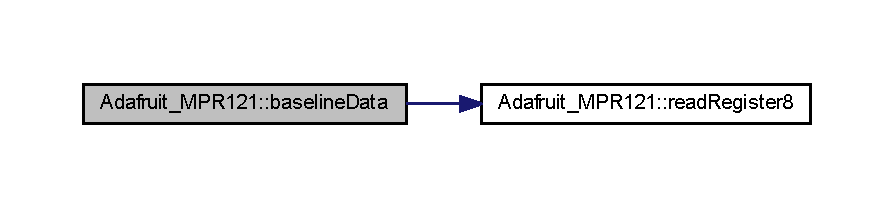
\includegraphics[width=350pt]{d9/d2e/class_adafruit___m_p_r121_a663d5e60aeb04b06697b2c40a33b40f0_cgraph}
\end{center}
\end{figure}
\mbox{\Hypertarget{class_adafruit___m_p_r121_ae269064c42ced60c7450eab53ada5eee}\label{class_adafruit___m_p_r121_ae269064c42ced60c7450eab53ada5eee}} 
\index{Adafruit\+\_\+\+M\+P\+R121@{Adafruit\+\_\+\+M\+P\+R121}!begin@{begin}}
\index{begin@{begin}!Adafruit\+\_\+\+M\+P\+R121@{Adafruit\+\_\+\+M\+P\+R121}}
\subsubsection{\texorpdfstring{begin()}{begin()}}
{\footnotesize\ttfamily boolean Adafruit\+\_\+\+M\+P\+R121\+::begin (\begin{DoxyParamCaption}\item[{uint8\+\_\+t}]{i2caddr = {\ttfamily \hyperlink{_adafruit___m_p_r121_8h_aa4a9474e42d9c498f600c9ad8781f714}{M\+P\+R121\+\_\+\+I2\+C\+A\+D\+D\+R\+\_\+\+D\+E\+F\+A\+U\+LT}} }\end{DoxyParamCaption})}

Here is the call graph for this function\+:
\nopagebreak
\begin{figure}[H]
\begin{center}
\leavevmode
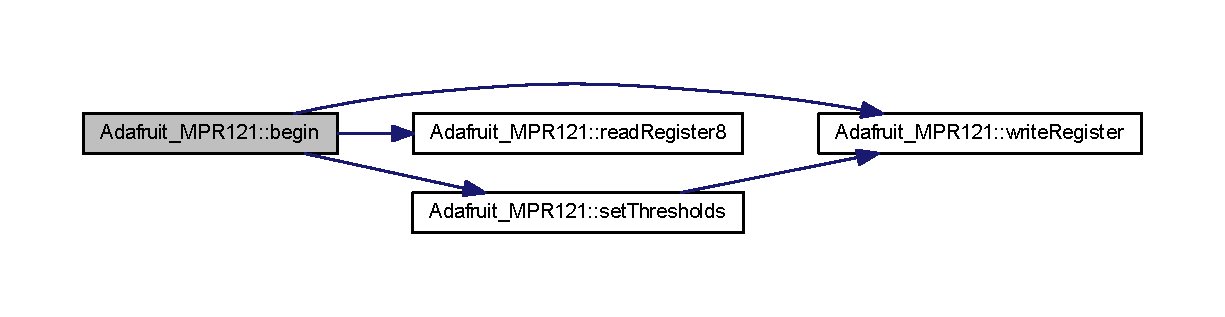
\includegraphics[width=350pt]{d9/d2e/class_adafruit___m_p_r121_ae269064c42ced60c7450eab53ada5eee_cgraph}
\end{center}
\end{figure}
\mbox{\Hypertarget{class_adafruit___m_p_r121_aa5bda4ff04ee361d857b80d95bddbbdb}\label{class_adafruit___m_p_r121_aa5bda4ff04ee361d857b80d95bddbbdb}} 
\index{Adafruit\+\_\+\+M\+P\+R121@{Adafruit\+\_\+\+M\+P\+R121}!filtered\+Data@{filtered\+Data}}
\index{filtered\+Data@{filtered\+Data}!Adafruit\+\_\+\+M\+P\+R121@{Adafruit\+\_\+\+M\+P\+R121}}
\subsubsection{\texorpdfstring{filtered\+Data()}{filteredData()}}
{\footnotesize\ttfamily uint16\+\_\+t Adafruit\+\_\+\+M\+P\+R121\+::filtered\+Data (\begin{DoxyParamCaption}\item[{uint8\+\_\+t}]{t }\end{DoxyParamCaption})}

Here is the call graph for this function\+:
\nopagebreak
\begin{figure}[H]
\begin{center}
\leavevmode
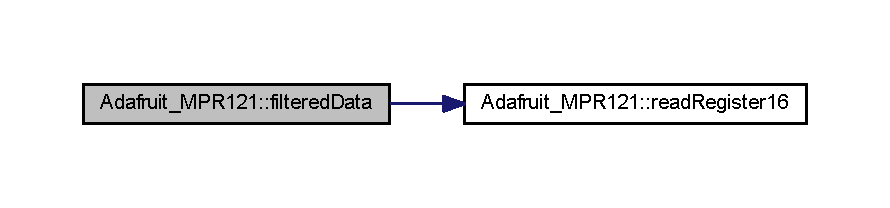
\includegraphics[width=350pt]{d9/d2e/class_adafruit___m_p_r121_aa5bda4ff04ee361d857b80d95bddbbdb_cgraph}
\end{center}
\end{figure}
\mbox{\Hypertarget{class_adafruit___m_p_r121_a171bf9f465d96819293657a589450e61}\label{class_adafruit___m_p_r121_a171bf9f465d96819293657a589450e61}} 
\index{Adafruit\+\_\+\+M\+P\+R121@{Adafruit\+\_\+\+M\+P\+R121}!read\+Register16@{read\+Register16}}
\index{read\+Register16@{read\+Register16}!Adafruit\+\_\+\+M\+P\+R121@{Adafruit\+\_\+\+M\+P\+R121}}
\subsubsection{\texorpdfstring{read\+Register16()}{readRegister16()}}
{\footnotesize\ttfamily uint16\+\_\+t Adafruit\+\_\+\+M\+P\+R121\+::read\+Register16 (\begin{DoxyParamCaption}\item[{uint8\+\_\+t}]{reg }\end{DoxyParamCaption})}

Here is the caller graph for this function\+:
\nopagebreak
\begin{figure}[H]
\begin{center}
\leavevmode
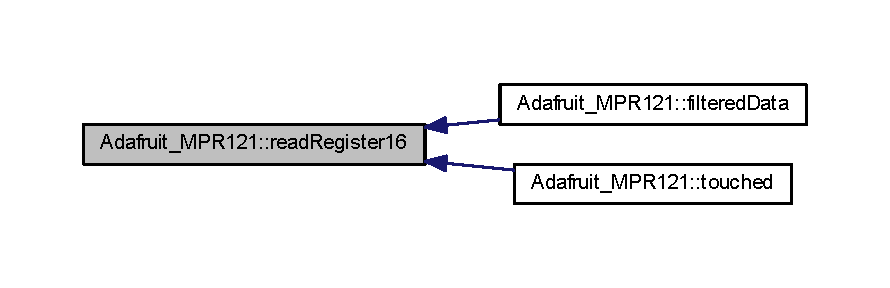
\includegraphics[width=350pt]{d9/d2e/class_adafruit___m_p_r121_a171bf9f465d96819293657a589450e61_icgraph}
\end{center}
\end{figure}
\mbox{\Hypertarget{class_adafruit___m_p_r121_a344c416d709121094a21d6892e23d28e}\label{class_adafruit___m_p_r121_a344c416d709121094a21d6892e23d28e}} 
\index{Adafruit\+\_\+\+M\+P\+R121@{Adafruit\+\_\+\+M\+P\+R121}!read\+Register8@{read\+Register8}}
\index{read\+Register8@{read\+Register8}!Adafruit\+\_\+\+M\+P\+R121@{Adafruit\+\_\+\+M\+P\+R121}}
\subsubsection{\texorpdfstring{read\+Register8()}{readRegister8()}}
{\footnotesize\ttfamily uint8\+\_\+t Adafruit\+\_\+\+M\+P\+R121\+::read\+Register8 (\begin{DoxyParamCaption}\item[{uint8\+\_\+t}]{reg }\end{DoxyParamCaption})}

Here is the caller graph for this function\+:
\nopagebreak
\begin{figure}[H]
\begin{center}
\leavevmode
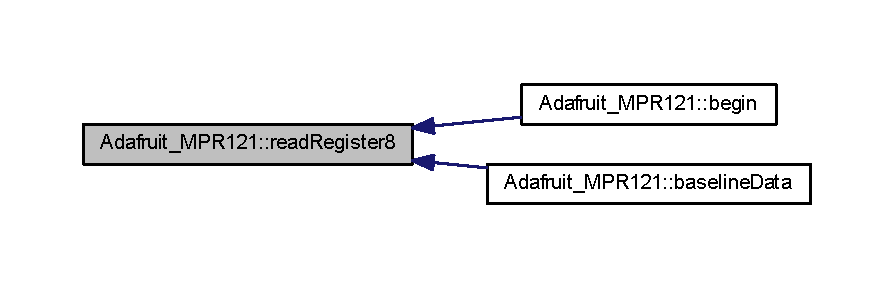
\includegraphics[width=350pt]{d9/d2e/class_adafruit___m_p_r121_a344c416d709121094a21d6892e23d28e_icgraph}
\end{center}
\end{figure}
\mbox{\Hypertarget{class_adafruit___m_p_r121_a8588eabc494059b6fe5231b8dd2be416}\label{class_adafruit___m_p_r121_a8588eabc494059b6fe5231b8dd2be416}} 
\index{Adafruit\+\_\+\+M\+P\+R121@{Adafruit\+\_\+\+M\+P\+R121}!set\+Thresholds@{set\+Thresholds}}
\index{set\+Thresholds@{set\+Thresholds}!Adafruit\+\_\+\+M\+P\+R121@{Adafruit\+\_\+\+M\+P\+R121}}
\subsubsection{\texorpdfstring{set\+Thresholds()}{setThresholds()}}
{\footnotesize\ttfamily void Adafruit\+\_\+\+M\+P\+R121\+::set\+Thresholds (\begin{DoxyParamCaption}\item[{uint8\+\_\+t}]{touch,  }\item[{uint8\+\_\+t}]{release }\end{DoxyParamCaption})}

Here is the call graph for this function\+:
\nopagebreak
\begin{figure}[H]
\begin{center}
\leavevmode
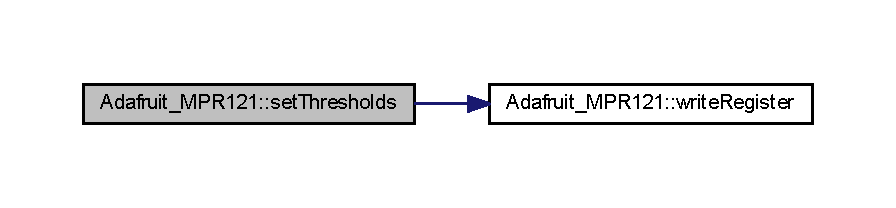
\includegraphics[width=350pt]{d9/d2e/class_adafruit___m_p_r121_a8588eabc494059b6fe5231b8dd2be416_cgraph}
\end{center}
\end{figure}
Here is the caller graph for this function\+:
\nopagebreak
\begin{figure}[H]
\begin{center}
\leavevmode
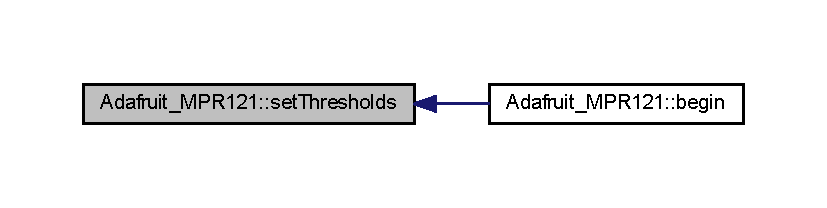
\includegraphics[width=350pt]{d9/d2e/class_adafruit___m_p_r121_a8588eabc494059b6fe5231b8dd2be416_icgraph}
\end{center}
\end{figure}
\mbox{\Hypertarget{class_adafruit___m_p_r121_a08b26f327e99b6f205df8907eafcab4c}\label{class_adafruit___m_p_r121_a08b26f327e99b6f205df8907eafcab4c}} 
\index{Adafruit\+\_\+\+M\+P\+R121@{Adafruit\+\_\+\+M\+P\+R121}!touched@{touched}}
\index{touched@{touched}!Adafruit\+\_\+\+M\+P\+R121@{Adafruit\+\_\+\+M\+P\+R121}}
\subsubsection{\texorpdfstring{touched()}{touched()}}
{\footnotesize\ttfamily uint16\+\_\+t Adafruit\+\_\+\+M\+P\+R121\+::touched (\begin{DoxyParamCaption}\item[{void}]{ }\end{DoxyParamCaption})}

Here is the call graph for this function\+:
\nopagebreak
\begin{figure}[H]
\begin{center}
\leavevmode
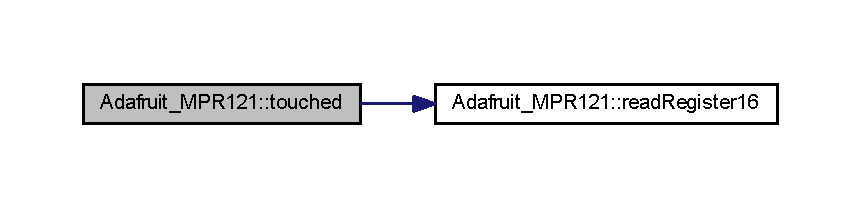
\includegraphics[width=350pt]{d9/d2e/class_adafruit___m_p_r121_a08b26f327e99b6f205df8907eafcab4c_cgraph}
\end{center}
\end{figure}
\mbox{\Hypertarget{class_adafruit___m_p_r121_a5dce866e817cfc15933e56b8dc679a13}\label{class_adafruit___m_p_r121_a5dce866e817cfc15933e56b8dc679a13}} 
\index{Adafruit\+\_\+\+M\+P\+R121@{Adafruit\+\_\+\+M\+P\+R121}!write\+Register@{write\+Register}}
\index{write\+Register@{write\+Register}!Adafruit\+\_\+\+M\+P\+R121@{Adafruit\+\_\+\+M\+P\+R121}}
\subsubsection{\texorpdfstring{write\+Register()}{writeRegister()}}
{\footnotesize\ttfamily void Adafruit\+\_\+\+M\+P\+R121\+::write\+Register (\begin{DoxyParamCaption}\item[{uint8\+\_\+t}]{reg,  }\item[{uint8\+\_\+t}]{value }\end{DoxyParamCaption})}



Writes 8-\/bits to the specified destination register. 

Here is the caller graph for this function\+:
\nopagebreak
\begin{figure}[H]
\begin{center}
\leavevmode
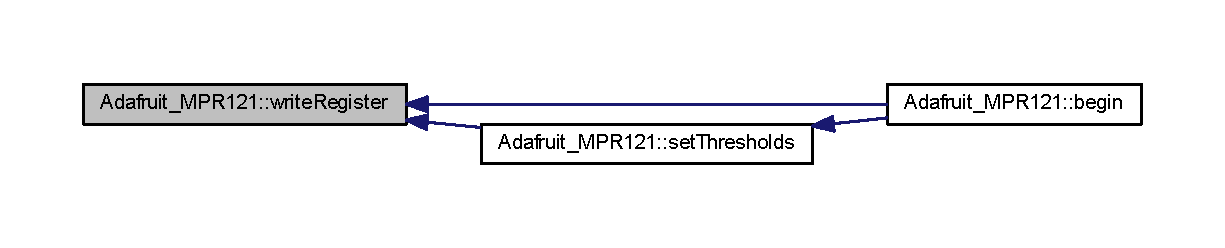
\includegraphics[width=350pt]{d9/d2e/class_adafruit___m_p_r121_a5dce866e817cfc15933e56b8dc679a13_icgraph}
\end{center}
\end{figure}


\subsection{Member Data Documentation}
\mbox{\Hypertarget{class_adafruit___m_p_r121_aff6b909093cf5eca8217990625c860fe}\label{class_adafruit___m_p_r121_aff6b909093cf5eca8217990625c860fe}} 
\index{Adafruit\+\_\+\+M\+P\+R121@{Adafruit\+\_\+\+M\+P\+R121}!release@{release}}
\index{release@{release}!Adafruit\+\_\+\+M\+P\+R121@{Adafruit\+\_\+\+M\+P\+R121}}
\subsubsection{\texorpdfstring{release}{release}}
{\footnotesize\ttfamily uint8\+\_\+t Adafruit\+\_\+\+M\+P\+R121\+::release}



The documentation for this class was generated from the following files\+:\begin{DoxyCompactItemize}
\item 
\hyperlink{_adafruit___m_p_r121_8h}{Adafruit\+\_\+\+M\+P\+R121.\+h}\item 
\hyperlink{_adafruit___m_p_r121_8cpp}{Adafruit\+\_\+\+M\+P\+R121.\+cpp}\end{DoxyCompactItemize}

\hypertarget{class_adafruit___s_t7735}{}\section{Adafruit\+\_\+\+S\+T7735 Class Reference}
\label{class_adafruit___s_t7735}\index{Adafruit\+\_\+\+S\+T7735@{Adafruit\+\_\+\+S\+T7735}}


{\ttfamily \#include $<$Adafruit\+\_\+\+S\+T7735.\+h$>$}



Inheritance diagram for Adafruit\+\_\+\+S\+T7735\+:
\nopagebreak
\begin{figure}[H]
\begin{center}
\leavevmode
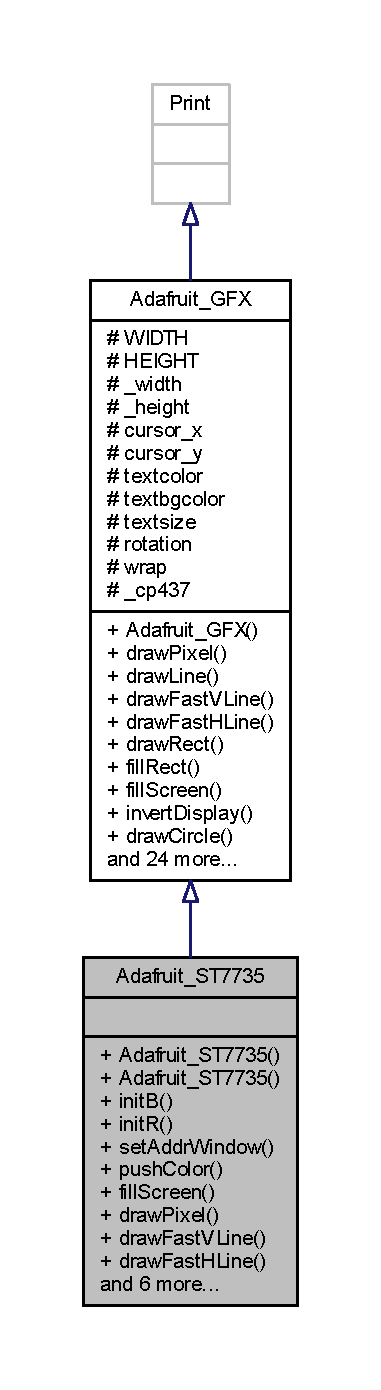
\includegraphics[height=550pt]{d5/d8b/class_adafruit___s_t7735__inherit__graph}
\end{center}
\end{figure}


Collaboration diagram for Adafruit\+\_\+\+S\+T7735\+:
\nopagebreak
\begin{figure}[H]
\begin{center}
\leavevmode
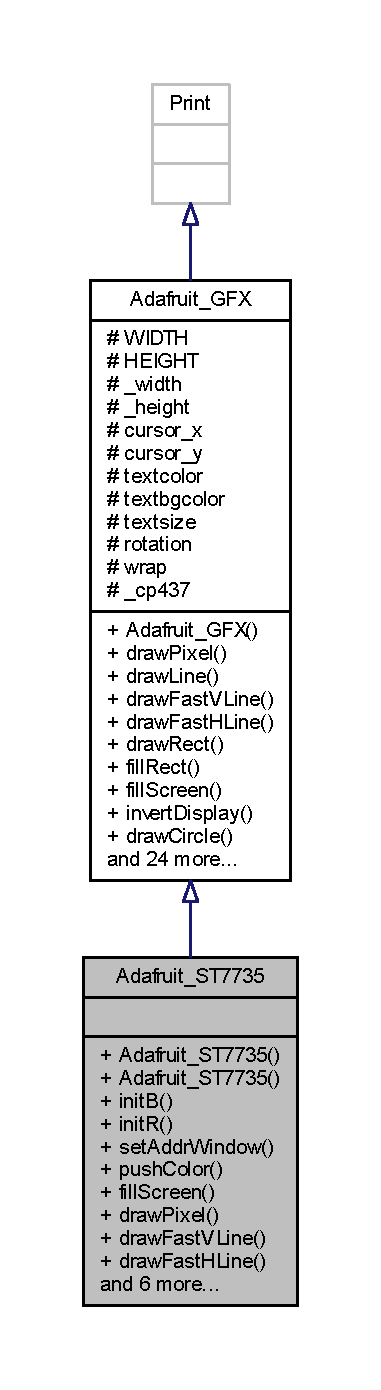
\includegraphics[height=550pt]{d0/d46/class_adafruit___s_t7735__coll__graph}
\end{center}
\end{figure}
\subsection*{Public Member Functions}
\begin{DoxyCompactItemize}
\item 
\hyperlink{class_adafruit___s_t7735_a920ee9f984e79dcddc6a60e306d9b446}{Adafruit\+\_\+\+S\+T7735} (int8\+\_\+t CS, int8\+\_\+t RS, int8\+\_\+t S\+ID, int8\+\_\+t S\+C\+LK, int8\+\_\+t R\+ST=-\/1)
\item 
\hyperlink{class_adafruit___s_t7735_aa1a91d0c5e8c2a28dbddffccea27dc9b}{Adafruit\+\_\+\+S\+T7735} (int8\+\_\+t CS, int8\+\_\+t RS, int8\+\_\+t R\+ST=-\/1)
\item 
void \hyperlink{class_adafruit___s_t7735_a71d8744ce7a27cd978ec64616d2ddae4}{initB} (void)
\item 
void \hyperlink{class_adafruit___s_t7735_a416b7a2b4748a90f8a33028522fa7504}{initR} (uint8\+\_\+t options=\hyperlink{_adafruit___s_t7735_8h_a8482c50b5e4da7ef9cc27ec7f16aa374}{I\+N\+I\+T\+R\+\_\+\+G\+R\+E\+E\+N\+T\+AB})
\item 
void \hyperlink{class_adafruit___s_t7735_ade48a8b2ba1e6375c5e3dbeaf84c44dd}{set\+Addr\+Window} (uint8\+\_\+t x0, uint8\+\_\+t y0, uint8\+\_\+t x1, uint8\+\_\+t y1)
\item 
void \hyperlink{class_adafruit___s_t7735_ac7e7977e3d664360f7f991cd7ae01035}{push\+Color} (uint16\+\_\+t color)
\item 
void \hyperlink{class_adafruit___s_t7735_af732d3d78239687718bb117de99418ca}{fill\+Screen} (uint16\+\_\+t color)
\item 
void \hyperlink{class_adafruit___s_t7735_af22a5ba7282850793f4943ba2d682af0}{draw\+Pixel} (int16\+\_\+t x, int16\+\_\+t y, uint16\+\_\+t color)
\item 
void \hyperlink{class_adafruit___s_t7735_a38de2e08911db493eb243ce2691e9c3a}{draw\+Fast\+V\+Line} (int16\+\_\+t x, int16\+\_\+t y, int16\+\_\+t h, uint16\+\_\+t color)
\item 
void \hyperlink{class_adafruit___s_t7735_ab2b8eb320bd19305c09b35be6d55d37e}{draw\+Fast\+H\+Line} (int16\+\_\+t x, int16\+\_\+t y, int16\+\_\+t w, uint16\+\_\+t color)
\item 
void \hyperlink{class_adafruit___s_t7735_a3556265c5b017cd2cdceb1f34e9bc421}{fill\+Rect} (int16\+\_\+t x, int16\+\_\+t y, int16\+\_\+t w, int16\+\_\+t h, uint16\+\_\+t color)
\item 
void \hyperlink{class_adafruit___s_t7735_aae15fa049e0aff62d58d8773182a87de}{set\+Rotation} (uint8\+\_\+t r)
\item 
void \hyperlink{class_adafruit___s_t7735_a2c7ac7e15a2b867273d4ddee5dde11c5}{invert\+Display} (boolean \hyperlink{dac___m_c_p4725_8cpp_ac2e790a754ca79a6e539135dc35f4fc0}{i})
\item 
uint16\+\_\+t \hyperlink{class_adafruit___s_t7735_aef9c4f90acb18082a51b18490feb3c0b}{Color565} (uint8\+\_\+t r, uint8\+\_\+t g, uint8\+\_\+t b)
\item 
void \hyperlink{class_adafruit___s_t7735_ac945c3d179185563dc2bfae09ac35375}{sleep} (void)
\item 
void \hyperlink{class_adafruit___s_t7735_aba13f16e02307bca2b422a8b8e16b754}{wake} (void)
\end{DoxyCompactItemize}
\subsection*{Additional Inherited Members}


\subsection{Constructor \& Destructor Documentation}
\mbox{\Hypertarget{class_adafruit___s_t7735_a920ee9f984e79dcddc6a60e306d9b446}\label{class_adafruit___s_t7735_a920ee9f984e79dcddc6a60e306d9b446}} 
\index{Adafruit\+\_\+\+S\+T7735@{Adafruit\+\_\+\+S\+T7735}!Adafruit\+\_\+\+S\+T7735@{Adafruit\+\_\+\+S\+T7735}}
\index{Adafruit\+\_\+\+S\+T7735@{Adafruit\+\_\+\+S\+T7735}!Adafruit\+\_\+\+S\+T7735@{Adafruit\+\_\+\+S\+T7735}}
\subsubsection{\texorpdfstring{Adafruit\+\_\+\+S\+T7735()}{Adafruit\_ST7735()}\hspace{0.1cm}{\footnotesize\ttfamily [1/2]}}
{\footnotesize\ttfamily Adafruit\+\_\+\+S\+T7735\+::\+Adafruit\+\_\+\+S\+T7735 (\begin{DoxyParamCaption}\item[{int8\+\_\+t}]{CS,  }\item[{int8\+\_\+t}]{RS,  }\item[{int8\+\_\+t}]{S\+ID,  }\item[{int8\+\_\+t}]{S\+C\+LK,  }\item[{int8\+\_\+t}]{R\+ST = {\ttfamily -\/1} }\end{DoxyParamCaption})}

\mbox{\Hypertarget{class_adafruit___s_t7735_aa1a91d0c5e8c2a28dbddffccea27dc9b}\label{class_adafruit___s_t7735_aa1a91d0c5e8c2a28dbddffccea27dc9b}} 
\index{Adafruit\+\_\+\+S\+T7735@{Adafruit\+\_\+\+S\+T7735}!Adafruit\+\_\+\+S\+T7735@{Adafruit\+\_\+\+S\+T7735}}
\index{Adafruit\+\_\+\+S\+T7735@{Adafruit\+\_\+\+S\+T7735}!Adafruit\+\_\+\+S\+T7735@{Adafruit\+\_\+\+S\+T7735}}
\subsubsection{\texorpdfstring{Adafruit\+\_\+\+S\+T7735()}{Adafruit\_ST7735()}\hspace{0.1cm}{\footnotesize\ttfamily [2/2]}}
{\footnotesize\ttfamily Adafruit\+\_\+\+S\+T7735\+::\+Adafruit\+\_\+\+S\+T7735 (\begin{DoxyParamCaption}\item[{int8\+\_\+t}]{CS,  }\item[{int8\+\_\+t}]{RS,  }\item[{int8\+\_\+t}]{R\+ST = {\ttfamily -\/1} }\end{DoxyParamCaption})}



\subsection{Member Function Documentation}
\mbox{\Hypertarget{class_adafruit___s_t7735_aef9c4f90acb18082a51b18490feb3c0b}\label{class_adafruit___s_t7735_aef9c4f90acb18082a51b18490feb3c0b}} 
\index{Adafruit\+\_\+\+S\+T7735@{Adafruit\+\_\+\+S\+T7735}!Color565@{Color565}}
\index{Color565@{Color565}!Adafruit\+\_\+\+S\+T7735@{Adafruit\+\_\+\+S\+T7735}}
\subsubsection{\texorpdfstring{Color565()}{Color565()}}
{\footnotesize\ttfamily uint16\+\_\+t Adafruit\+\_\+\+S\+T7735\+::\+Color565 (\begin{DoxyParamCaption}\item[{uint8\+\_\+t}]{r,  }\item[{uint8\+\_\+t}]{g,  }\item[{uint8\+\_\+t}]{b }\end{DoxyParamCaption})}

\mbox{\Hypertarget{class_adafruit___s_t7735_ab2b8eb320bd19305c09b35be6d55d37e}\label{class_adafruit___s_t7735_ab2b8eb320bd19305c09b35be6d55d37e}} 
\index{Adafruit\+\_\+\+S\+T7735@{Adafruit\+\_\+\+S\+T7735}!draw\+Fast\+H\+Line@{draw\+Fast\+H\+Line}}
\index{draw\+Fast\+H\+Line@{draw\+Fast\+H\+Line}!Adafruit\+\_\+\+S\+T7735@{Adafruit\+\_\+\+S\+T7735}}
\subsubsection{\texorpdfstring{draw\+Fast\+H\+Line()}{drawFastHLine()}}
{\footnotesize\ttfamily void Adafruit\+\_\+\+S\+T7735\+::draw\+Fast\+H\+Line (\begin{DoxyParamCaption}\item[{int16\+\_\+t}]{x,  }\item[{int16\+\_\+t}]{y,  }\item[{int16\+\_\+t}]{w,  }\item[{uint16\+\_\+t}]{color }\end{DoxyParamCaption})}

Here is the call graph for this function\+:
\nopagebreak
\begin{figure}[H]
\begin{center}
\leavevmode
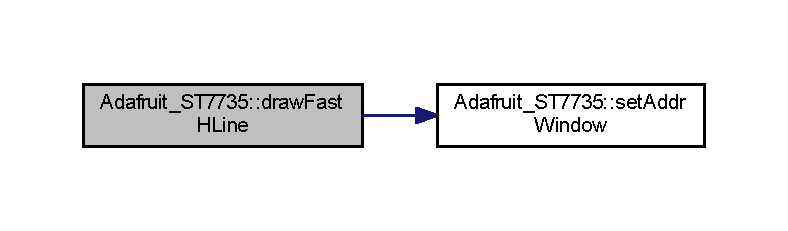
\includegraphics[width=350pt]{dd/dee/class_adafruit___s_t7735_ab2b8eb320bd19305c09b35be6d55d37e_cgraph}
\end{center}
\end{figure}
\mbox{\Hypertarget{class_adafruit___s_t7735_a38de2e08911db493eb243ce2691e9c3a}\label{class_adafruit___s_t7735_a38de2e08911db493eb243ce2691e9c3a}} 
\index{Adafruit\+\_\+\+S\+T7735@{Adafruit\+\_\+\+S\+T7735}!draw\+Fast\+V\+Line@{draw\+Fast\+V\+Line}}
\index{draw\+Fast\+V\+Line@{draw\+Fast\+V\+Line}!Adafruit\+\_\+\+S\+T7735@{Adafruit\+\_\+\+S\+T7735}}
\subsubsection{\texorpdfstring{draw\+Fast\+V\+Line()}{drawFastVLine()}}
{\footnotesize\ttfamily void Adafruit\+\_\+\+S\+T7735\+::draw\+Fast\+V\+Line (\begin{DoxyParamCaption}\item[{int16\+\_\+t}]{x,  }\item[{int16\+\_\+t}]{y,  }\item[{int16\+\_\+t}]{h,  }\item[{uint16\+\_\+t}]{color }\end{DoxyParamCaption})}

Here is the call graph for this function\+:
\nopagebreak
\begin{figure}[H]
\begin{center}
\leavevmode
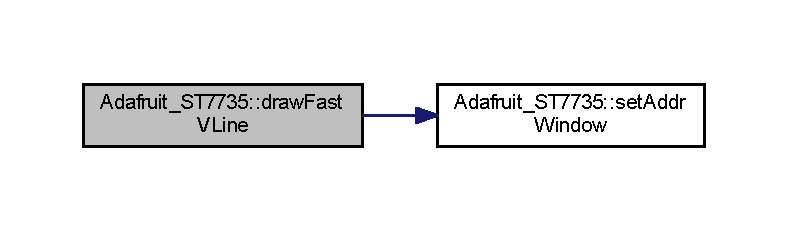
\includegraphics[width=350pt]{dd/dee/class_adafruit___s_t7735_a38de2e08911db493eb243ce2691e9c3a_cgraph}
\end{center}
\end{figure}
\mbox{\Hypertarget{class_adafruit___s_t7735_af22a5ba7282850793f4943ba2d682af0}\label{class_adafruit___s_t7735_af22a5ba7282850793f4943ba2d682af0}} 
\index{Adafruit\+\_\+\+S\+T7735@{Adafruit\+\_\+\+S\+T7735}!draw\+Pixel@{draw\+Pixel}}
\index{draw\+Pixel@{draw\+Pixel}!Adafruit\+\_\+\+S\+T7735@{Adafruit\+\_\+\+S\+T7735}}
\subsubsection{\texorpdfstring{draw\+Pixel()}{drawPixel()}}
{\footnotesize\ttfamily void Adafruit\+\_\+\+S\+T7735\+::draw\+Pixel (\begin{DoxyParamCaption}\item[{int16\+\_\+t}]{x,  }\item[{int16\+\_\+t}]{y,  }\item[{uint16\+\_\+t}]{color }\end{DoxyParamCaption})\hspace{0.3cm}{\ttfamily [virtual]}}



Implements \hyperlink{class_adafruit___g_f_x_ab7fbf72885c873266f9c7eb53b5c8896}{Adafruit\+\_\+\+G\+FX}.

Here is the call graph for this function\+:
\nopagebreak
\begin{figure}[H]
\begin{center}
\leavevmode
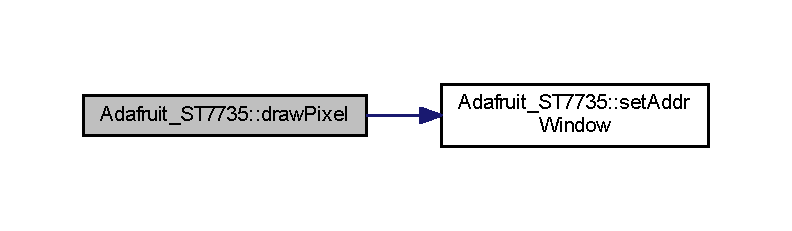
\includegraphics[width=350pt]{dd/dee/class_adafruit___s_t7735_af22a5ba7282850793f4943ba2d682af0_cgraph}
\end{center}
\end{figure}
\mbox{\Hypertarget{class_adafruit___s_t7735_a3556265c5b017cd2cdceb1f34e9bc421}\label{class_adafruit___s_t7735_a3556265c5b017cd2cdceb1f34e9bc421}} 
\index{Adafruit\+\_\+\+S\+T7735@{Adafruit\+\_\+\+S\+T7735}!fill\+Rect@{fill\+Rect}}
\index{fill\+Rect@{fill\+Rect}!Adafruit\+\_\+\+S\+T7735@{Adafruit\+\_\+\+S\+T7735}}
\subsubsection{\texorpdfstring{fill\+Rect()}{fillRect()}}
{\footnotesize\ttfamily void Adafruit\+\_\+\+S\+T7735\+::fill\+Rect (\begin{DoxyParamCaption}\item[{int16\+\_\+t}]{x,  }\item[{int16\+\_\+t}]{y,  }\item[{int16\+\_\+t}]{w,  }\item[{int16\+\_\+t}]{h,  }\item[{uint16\+\_\+t}]{color }\end{DoxyParamCaption})}

Here is the call graph for this function\+:
\nopagebreak
\begin{figure}[H]
\begin{center}
\leavevmode
\includegraphics[width=350pt]{dd/dee/class_adafruit___s_t7735_a3556265c5b017cd2cdceb1f34e9bc421_cgraph}
\end{center}
\end{figure}
Here is the caller graph for this function\+:
\nopagebreak
\begin{figure}[H]
\begin{center}
\leavevmode
\includegraphics[width=350pt]{dd/dee/class_adafruit___s_t7735_a3556265c5b017cd2cdceb1f34e9bc421_icgraph}
\end{center}
\end{figure}
\mbox{\Hypertarget{class_adafruit___s_t7735_af732d3d78239687718bb117de99418ca}\label{class_adafruit___s_t7735_af732d3d78239687718bb117de99418ca}} 
\index{Adafruit\+\_\+\+S\+T7735@{Adafruit\+\_\+\+S\+T7735}!fill\+Screen@{fill\+Screen}}
\index{fill\+Screen@{fill\+Screen}!Adafruit\+\_\+\+S\+T7735@{Adafruit\+\_\+\+S\+T7735}}
\subsubsection{\texorpdfstring{fill\+Screen()}{fillScreen()}}
{\footnotesize\ttfamily void Adafruit\+\_\+\+S\+T7735\+::fill\+Screen (\begin{DoxyParamCaption}\item[{uint16\+\_\+t}]{color }\end{DoxyParamCaption})}

Here is the call graph for this function\+:
\nopagebreak
\begin{figure}[H]
\begin{center}
\leavevmode
\includegraphics[width=350pt]{dd/dee/class_adafruit___s_t7735_af732d3d78239687718bb117de99418ca_cgraph}
\end{center}
\end{figure}
Here is the caller graph for this function\+:
\nopagebreak
\begin{figure}[H]
\begin{center}
\leavevmode
\includegraphics[width=350pt]{dd/dee/class_adafruit___s_t7735_af732d3d78239687718bb117de99418ca_icgraph}
\end{center}
\end{figure}
\mbox{\Hypertarget{class_adafruit___s_t7735_a71d8744ce7a27cd978ec64616d2ddae4}\label{class_adafruit___s_t7735_a71d8744ce7a27cd978ec64616d2ddae4}} 
\index{Adafruit\+\_\+\+S\+T7735@{Adafruit\+\_\+\+S\+T7735}!initB@{initB}}
\index{initB@{initB}!Adafruit\+\_\+\+S\+T7735@{Adafruit\+\_\+\+S\+T7735}}
\subsubsection{\texorpdfstring{init\+B()}{initB()}}
{\footnotesize\ttfamily void Adafruit\+\_\+\+S\+T7735\+::initB (\begin{DoxyParamCaption}\item[{void}]{ }\end{DoxyParamCaption})}

\mbox{\Hypertarget{class_adafruit___s_t7735_a416b7a2b4748a90f8a33028522fa7504}\label{class_adafruit___s_t7735_a416b7a2b4748a90f8a33028522fa7504}} 
\index{Adafruit\+\_\+\+S\+T7735@{Adafruit\+\_\+\+S\+T7735}!initR@{initR}}
\index{initR@{initR}!Adafruit\+\_\+\+S\+T7735@{Adafruit\+\_\+\+S\+T7735}}
\subsubsection{\texorpdfstring{init\+R()}{initR()}}
{\footnotesize\ttfamily void Adafruit\+\_\+\+S\+T7735\+::initR (\begin{DoxyParamCaption}\item[{uint8\+\_\+t}]{options = {\ttfamily \hyperlink{_adafruit___s_t7735_8h_a8482c50b5e4da7ef9cc27ec7f16aa374}{I\+N\+I\+T\+R\+\_\+\+G\+R\+E\+E\+N\+T\+AB}} }\end{DoxyParamCaption})}

\mbox{\Hypertarget{class_adafruit___s_t7735_a2c7ac7e15a2b867273d4ddee5dde11c5}\label{class_adafruit___s_t7735_a2c7ac7e15a2b867273d4ddee5dde11c5}} 
\index{Adafruit\+\_\+\+S\+T7735@{Adafruit\+\_\+\+S\+T7735}!invert\+Display@{invert\+Display}}
\index{invert\+Display@{invert\+Display}!Adafruit\+\_\+\+S\+T7735@{Adafruit\+\_\+\+S\+T7735}}
\subsubsection{\texorpdfstring{invert\+Display()}{invertDisplay()}}
{\footnotesize\ttfamily void Adafruit\+\_\+\+S\+T7735\+::invert\+Display (\begin{DoxyParamCaption}\item[{boolean}]{i }\end{DoxyParamCaption})}

\mbox{\Hypertarget{class_adafruit___s_t7735_ac7e7977e3d664360f7f991cd7ae01035}\label{class_adafruit___s_t7735_ac7e7977e3d664360f7f991cd7ae01035}} 
\index{Adafruit\+\_\+\+S\+T7735@{Adafruit\+\_\+\+S\+T7735}!push\+Color@{push\+Color}}
\index{push\+Color@{push\+Color}!Adafruit\+\_\+\+S\+T7735@{Adafruit\+\_\+\+S\+T7735}}
\subsubsection{\texorpdfstring{push\+Color()}{pushColor()}}
{\footnotesize\ttfamily void Adafruit\+\_\+\+S\+T7735\+::push\+Color (\begin{DoxyParamCaption}\item[{uint16\+\_\+t}]{color }\end{DoxyParamCaption})}

\mbox{\Hypertarget{class_adafruit___s_t7735_ade48a8b2ba1e6375c5e3dbeaf84c44dd}\label{class_adafruit___s_t7735_ade48a8b2ba1e6375c5e3dbeaf84c44dd}} 
\index{Adafruit\+\_\+\+S\+T7735@{Adafruit\+\_\+\+S\+T7735}!set\+Addr\+Window@{set\+Addr\+Window}}
\index{set\+Addr\+Window@{set\+Addr\+Window}!Adafruit\+\_\+\+S\+T7735@{Adafruit\+\_\+\+S\+T7735}}
\subsubsection{\texorpdfstring{set\+Addr\+Window()}{setAddrWindow()}}
{\footnotesize\ttfamily void Adafruit\+\_\+\+S\+T7735\+::set\+Addr\+Window (\begin{DoxyParamCaption}\item[{uint8\+\_\+t}]{x0,  }\item[{uint8\+\_\+t}]{y0,  }\item[{uint8\+\_\+t}]{x1,  }\item[{uint8\+\_\+t}]{y1 }\end{DoxyParamCaption})}

Here is the caller graph for this function\+:
\nopagebreak
\begin{figure}[H]
\begin{center}
\leavevmode
\includegraphics[width=350pt]{dd/dee/class_adafruit___s_t7735_ade48a8b2ba1e6375c5e3dbeaf84c44dd_icgraph}
\end{center}
\end{figure}
\mbox{\Hypertarget{class_adafruit___s_t7735_aae15fa049e0aff62d58d8773182a87de}\label{class_adafruit___s_t7735_aae15fa049e0aff62d58d8773182a87de}} 
\index{Adafruit\+\_\+\+S\+T7735@{Adafruit\+\_\+\+S\+T7735}!set\+Rotation@{set\+Rotation}}
\index{set\+Rotation@{set\+Rotation}!Adafruit\+\_\+\+S\+T7735@{Adafruit\+\_\+\+S\+T7735}}
\subsubsection{\texorpdfstring{set\+Rotation()}{setRotation()}}
{\footnotesize\ttfamily void Adafruit\+\_\+\+S\+T7735\+::set\+Rotation (\begin{DoxyParamCaption}\item[{uint8\+\_\+t}]{r }\end{DoxyParamCaption})}

\mbox{\Hypertarget{class_adafruit___s_t7735_ac945c3d179185563dc2bfae09ac35375}\label{class_adafruit___s_t7735_ac945c3d179185563dc2bfae09ac35375}} 
\index{Adafruit\+\_\+\+S\+T7735@{Adafruit\+\_\+\+S\+T7735}!sleep@{sleep}}
\index{sleep@{sleep}!Adafruit\+\_\+\+S\+T7735@{Adafruit\+\_\+\+S\+T7735}}
\subsubsection{\texorpdfstring{sleep()}{sleep()}}
{\footnotesize\ttfamily void Adafruit\+\_\+\+S\+T7735\+::sleep (\begin{DoxyParamCaption}\item[{void}]{ }\end{DoxyParamCaption})\hspace{0.3cm}{\ttfamily [inline]}}

\mbox{\Hypertarget{class_adafruit___s_t7735_aba13f16e02307bca2b422a8b8e16b754}\label{class_adafruit___s_t7735_aba13f16e02307bca2b422a8b8e16b754}} 
\index{Adafruit\+\_\+\+S\+T7735@{Adafruit\+\_\+\+S\+T7735}!wake@{wake}}
\index{wake@{wake}!Adafruit\+\_\+\+S\+T7735@{Adafruit\+\_\+\+S\+T7735}}
\subsubsection{\texorpdfstring{wake()}{wake()}}
{\footnotesize\ttfamily void Adafruit\+\_\+\+S\+T7735\+::wake (\begin{DoxyParamCaption}\item[{void}]{ }\end{DoxyParamCaption})\hspace{0.3cm}{\ttfamily [inline]}}



The documentation for this class was generated from the following files\+:\begin{DoxyCompactItemize}
\item 
\hyperlink{_adafruit___s_t7735_8h}{Adafruit\+\_\+\+S\+T7735.\+h}\item 
\hyperlink{_adafruit___s_t7735_8cpp}{Adafruit\+\_\+\+S\+T7735.\+cpp}\end{DoxyCompactItemize}

\hypertarget{class_button}{}\section{Button Class Reference}
\label{class_button}\index{Button@{Button}}


{\ttfamily \#include $<$button.\+h$>$}



Collaboration diagram for Button\+:
\nopagebreak
\begin{figure}[H]
\begin{center}
\leavevmode
\includegraphics[width=169pt]{db/d33/class_button__coll__graph}
\end{center}
\end{figure}
\subsection*{Public Member Functions}
\begin{DoxyCompactItemize}
\item 
\hyperlink{class_button_a62bf06885bb7e8e8e10320394469142e}{Button} (uint8\+\_\+t pin)
\item 
\hyperlink{class_button_ad61b19bac87236f03f72f5debce40057}{Button} (uint8\+\_\+t pin, uint32\+\_\+t db\+Time)
\item 
\hyperlink{class_button_afed59e35f623f232ae04a892127a0738}{Button} (uint8\+\_\+t pin, uint8\+\_\+t pu\+Enable, uint8\+\_\+t invert, uint32\+\_\+t db\+Time)
\item 
uint8\+\_\+t \hyperlink{class_button_a5f5c0d23ab0e5387b861e68019a7e85d}{read} ()
\item 
uint8\+\_\+t \hyperlink{class_button_adc52c28d5eecbb08818e4a701e346fb0}{is\+Pressed} ()
\item 
uint8\+\_\+t \hyperlink{class_button_a7bf938a70dee91015b044e434fc9499b}{is\+Released} ()
\item 
uint8\+\_\+t \hyperlink{class_button_a3496a1689b2b2f5635d5c7716f38ec43}{was\+Pressed} ()
\item 
uint8\+\_\+t \hyperlink{class_button_a79164a7fd70f08cb8c3930e8c06b9190}{was\+Released} ()
\item 
uint8\+\_\+t \hyperlink{class_button_a11b97b9e73881e876724ddeedac716f9}{pressed\+For} (uint32\+\_\+t ms)
\item 
uint8\+\_\+t \hyperlink{class_button_a805e542eaf9976b7c1afaf3dfecc13a5}{released\+For} (uint32\+\_\+t ms)
\item 
uint32\+\_\+t \hyperlink{class_button_a6880ef962e03d55216d79217e7473bd2}{last\+Change} ()
\end{DoxyCompactItemize}


\subsection{Constructor \& Destructor Documentation}
\mbox{\Hypertarget{class_button_a62bf06885bb7e8e8e10320394469142e}\label{class_button_a62bf06885bb7e8e8e10320394469142e}} 
\index{Button@{Button}!Button@{Button}}
\index{Button@{Button}!Button@{Button}}
\subsubsection{\texorpdfstring{Button()}{Button()}\hspace{0.1cm}{\footnotesize\ttfamily [1/3]}}
{\footnotesize\ttfamily Button\+::\+Button (\begin{DoxyParamCaption}\item[{uint8\+\_\+t}]{pin }\end{DoxyParamCaption})}

\mbox{\Hypertarget{class_button_ad61b19bac87236f03f72f5debce40057}\label{class_button_ad61b19bac87236f03f72f5debce40057}} 
\index{Button@{Button}!Button@{Button}}
\index{Button@{Button}!Button@{Button}}
\subsubsection{\texorpdfstring{Button()}{Button()}\hspace{0.1cm}{\footnotesize\ttfamily [2/3]}}
{\footnotesize\ttfamily Button\+::\+Button (\begin{DoxyParamCaption}\item[{uint8\+\_\+t}]{pin,  }\item[{uint32\+\_\+t}]{db\+Time }\end{DoxyParamCaption})}

\mbox{\Hypertarget{class_button_afed59e35f623f232ae04a892127a0738}\label{class_button_afed59e35f623f232ae04a892127a0738}} 
\index{Button@{Button}!Button@{Button}}
\index{Button@{Button}!Button@{Button}}
\subsubsection{\texorpdfstring{Button()}{Button()}\hspace{0.1cm}{\footnotesize\ttfamily [3/3]}}
{\footnotesize\ttfamily Button\+::\+Button (\begin{DoxyParamCaption}\item[{uint8\+\_\+t}]{pin,  }\item[{uint8\+\_\+t}]{pu\+Enable,  }\item[{uint8\+\_\+t}]{invert,  }\item[{uint32\+\_\+t}]{db\+Time }\end{DoxyParamCaption})}



\subsection{Member Function Documentation}
\mbox{\Hypertarget{class_button_adc52c28d5eecbb08818e4a701e346fb0}\label{class_button_adc52c28d5eecbb08818e4a701e346fb0}} 
\index{Button@{Button}!is\+Pressed@{is\+Pressed}}
\index{is\+Pressed@{is\+Pressed}!Button@{Button}}
\subsubsection{\texorpdfstring{is\+Pressed()}{isPressed()}}
{\footnotesize\ttfamily uint8\+\_\+t Button\+::is\+Pressed (\begin{DoxyParamCaption}\item[{void}]{ }\end{DoxyParamCaption})}

\mbox{\Hypertarget{class_button_a7bf938a70dee91015b044e434fc9499b}\label{class_button_a7bf938a70dee91015b044e434fc9499b}} 
\index{Button@{Button}!is\+Released@{is\+Released}}
\index{is\+Released@{is\+Released}!Button@{Button}}
\subsubsection{\texorpdfstring{is\+Released()}{isReleased()}}
{\footnotesize\ttfamily uint8\+\_\+t Button\+::is\+Released (\begin{DoxyParamCaption}\item[{void}]{ }\end{DoxyParamCaption})}

\mbox{\Hypertarget{class_button_a6880ef962e03d55216d79217e7473bd2}\label{class_button_a6880ef962e03d55216d79217e7473bd2}} 
\index{Button@{Button}!last\+Change@{last\+Change}}
\index{last\+Change@{last\+Change}!Button@{Button}}
\subsubsection{\texorpdfstring{last\+Change()}{lastChange()}}
{\footnotesize\ttfamily uint32\+\_\+t Button\+::last\+Change (\begin{DoxyParamCaption}\item[{void}]{ }\end{DoxyParamCaption})}

\mbox{\Hypertarget{class_button_a11b97b9e73881e876724ddeedac716f9}\label{class_button_a11b97b9e73881e876724ddeedac716f9}} 
\index{Button@{Button}!pressed\+For@{pressed\+For}}
\index{pressed\+For@{pressed\+For}!Button@{Button}}
\subsubsection{\texorpdfstring{pressed\+For()}{pressedFor()}}
{\footnotesize\ttfamily uint8\+\_\+t Button\+::pressed\+For (\begin{DoxyParamCaption}\item[{uint32\+\_\+t}]{ms }\end{DoxyParamCaption})}

\mbox{\Hypertarget{class_button_a5f5c0d23ab0e5387b861e68019a7e85d}\label{class_button_a5f5c0d23ab0e5387b861e68019a7e85d}} 
\index{Button@{Button}!read@{read}}
\index{read@{read}!Button@{Button}}
\subsubsection{\texorpdfstring{read()}{read()}}
{\footnotesize\ttfamily uint8\+\_\+t Button\+::read (\begin{DoxyParamCaption}\item[{void}]{ }\end{DoxyParamCaption})}

Here is the caller graph for this function\+:
\nopagebreak
\begin{figure}[H]
\begin{center}
\leavevmode
\includegraphics[width=350pt]{d4/d77/class_button_a5f5c0d23ab0e5387b861e68019a7e85d_icgraph}
\end{center}
\end{figure}
\mbox{\Hypertarget{class_button_a805e542eaf9976b7c1afaf3dfecc13a5}\label{class_button_a805e542eaf9976b7c1afaf3dfecc13a5}} 
\index{Button@{Button}!released\+For@{released\+For}}
\index{released\+For@{released\+For}!Button@{Button}}
\subsubsection{\texorpdfstring{released\+For()}{releasedFor()}}
{\footnotesize\ttfamily uint8\+\_\+t Button\+::released\+For (\begin{DoxyParamCaption}\item[{uint32\+\_\+t}]{ms }\end{DoxyParamCaption})}

\mbox{\Hypertarget{class_button_a3496a1689b2b2f5635d5c7716f38ec43}\label{class_button_a3496a1689b2b2f5635d5c7716f38ec43}} 
\index{Button@{Button}!was\+Pressed@{was\+Pressed}}
\index{was\+Pressed@{was\+Pressed}!Button@{Button}}
\subsubsection{\texorpdfstring{was\+Pressed()}{wasPressed()}}
{\footnotesize\ttfamily uint8\+\_\+t Button\+::was\+Pressed (\begin{DoxyParamCaption}\item[{void}]{ }\end{DoxyParamCaption})}

\mbox{\Hypertarget{class_button_a79164a7fd70f08cb8c3930e8c06b9190}\label{class_button_a79164a7fd70f08cb8c3930e8c06b9190}} 
\index{Button@{Button}!was\+Released@{was\+Released}}
\index{was\+Released@{was\+Released}!Button@{Button}}
\subsubsection{\texorpdfstring{was\+Released()}{wasReleased()}}
{\footnotesize\ttfamily uint8\+\_\+t Button\+::was\+Released (\begin{DoxyParamCaption}\item[{void}]{ }\end{DoxyParamCaption})}



The documentation for this class was generated from the following files\+:\begin{DoxyCompactItemize}
\item 
\hyperlink{button_8h}{button.\+h}\item 
\hyperlink{button_8cpp}{button.\+cpp}\end{DoxyCompactItemize}

\hypertarget{classdac___m_c_p4725}{}\section{dac\+\_\+\+M\+C\+P4725 Class Reference}
\label{classdac___m_c_p4725}\index{dac\+\_\+\+M\+C\+P4725@{dac\+\_\+\+M\+C\+P4725}}


{\ttfamily \#include $<$dac\+\_\+\+M\+C\+P4725.\+h$>$}



Collaboration diagram for dac\+\_\+\+M\+C\+P4725\+:
\nopagebreak
\begin{figure}[H]
\begin{center}
\leavevmode
\includegraphics[width=175pt]{d8/dde/classdac___m_c_p4725__coll__graph}
\end{center}
\end{figure}
\subsection*{Public Member Functions}
\begin{DoxyCompactItemize}
\item 
\hyperlink{classdac___m_c_p4725_a1963bacd207b3c9618485427a706bc86}{dac\+\_\+\+M\+C\+P4725} ()
\begin{DoxyCompactList}\small\item\em Instantiates a new M\+C\+P4725 class. \end{DoxyCompactList}\item 
void \hyperlink{classdac___m_c_p4725_ad2a4a3342f561821e76388ad3849a0a7}{begin} (uint8\+\_\+t a)
\begin{DoxyCompactList}\small\item\em Setups the HW. \end{DoxyCompactList}\item 
void \hyperlink{classdac___m_c_p4725_a93548cddb90bd4f58c4fc3b53516fd08}{set\+Voltage} (uint16\+\_\+t output, bool write\+E\+E\+P\+R\+OM)
\begin{DoxyCompactList}\small\item\em Sets the output voltage to a fraction of source vref. (Value can be 0..4095) \end{DoxyCompactList}\end{DoxyCompactItemize}


\subsection{Constructor \& Destructor Documentation}
\mbox{\Hypertarget{classdac___m_c_p4725_a1963bacd207b3c9618485427a706bc86}\label{classdac___m_c_p4725_a1963bacd207b3c9618485427a706bc86}} 
\index{dac\+\_\+\+M\+C\+P4725@{dac\+\_\+\+M\+C\+P4725}!dac\+\_\+\+M\+C\+P4725@{dac\+\_\+\+M\+C\+P4725}}
\index{dac\+\_\+\+M\+C\+P4725@{dac\+\_\+\+M\+C\+P4725}!dac\+\_\+\+M\+C\+P4725@{dac\+\_\+\+M\+C\+P4725}}
\subsubsection{\texorpdfstring{dac\+\_\+\+M\+C\+P4725()}{dac\_MCP4725()}}
{\footnotesize\ttfamily dac\+\_\+\+M\+C\+P4725\+::dac\+\_\+\+M\+C\+P4725 (\begin{DoxyParamCaption}{ }\end{DoxyParamCaption})}



Instantiates a new M\+C\+P4725 class. 



\subsection{Member Function Documentation}
\mbox{\Hypertarget{classdac___m_c_p4725_ad2a4a3342f561821e76388ad3849a0a7}\label{classdac___m_c_p4725_ad2a4a3342f561821e76388ad3849a0a7}} 
\index{dac\+\_\+\+M\+C\+P4725@{dac\+\_\+\+M\+C\+P4725}!begin@{begin}}
\index{begin@{begin}!dac\+\_\+\+M\+C\+P4725@{dac\+\_\+\+M\+C\+P4725}}
\subsubsection{\texorpdfstring{begin()}{begin()}}
{\footnotesize\ttfamily void dac\+\_\+\+M\+C\+P4725\+::begin (\begin{DoxyParamCaption}\item[{uint8\+\_\+t}]{a }\end{DoxyParamCaption})}



Setups the HW. 

\mbox{\Hypertarget{classdac___m_c_p4725_a93548cddb90bd4f58c4fc3b53516fd08}\label{classdac___m_c_p4725_a93548cddb90bd4f58c4fc3b53516fd08}} 
\index{dac\+\_\+\+M\+C\+P4725@{dac\+\_\+\+M\+C\+P4725}!set\+Voltage@{set\+Voltage}}
\index{set\+Voltage@{set\+Voltage}!dac\+\_\+\+M\+C\+P4725@{dac\+\_\+\+M\+C\+P4725}}
\subsubsection{\texorpdfstring{set\+Voltage()}{setVoltage()}}
{\footnotesize\ttfamily void dac\+\_\+\+M\+C\+P4725\+::set\+Voltage (\begin{DoxyParamCaption}\item[{uint16\+\_\+t}]{output,  }\item[{bool}]{write\+E\+E\+P\+R\+OM }\end{DoxyParamCaption})}



Sets the output voltage to a fraction of source vref. (Value can be 0..4095) 


\begin{DoxyParams}[1]{Parameters}
\mbox{\tt in}  & {\em output} & The 12-\/bit value representing the relationship between the D\+AC\textquotesingle{}s input voltage and its output voltage. \\
\hline
\mbox{\tt in}  & {\em write\+E\+E\+P\+R\+OM} & If this value is true, \textquotesingle{}output\textquotesingle{} will also be written to the M\+C\+P4725\textquotesingle{}s internal non-\/volatile memory, meaning that the D\+AC will retain the current voltage output after power-\/down or reset. \\
\hline
\end{DoxyParams}
Here is the caller graph for this function\+:
\nopagebreak
\begin{figure}[H]
\begin{center}
\leavevmode
\includegraphics[width=350pt]{d9/d4f/classdac___m_c_p4725_a93548cddb90bd4f58c4fc3b53516fd08_icgraph}
\end{center}
\end{figure}


The documentation for this class was generated from the following files\+:\begin{DoxyCompactItemize}
\item 
\hyperlink{dac___m_c_p4725_8h}{dac\+\_\+\+M\+C\+P4725.\+h}\item 
\hyperlink{dac___m_c_p4725_8cpp}{dac\+\_\+\+M\+C\+P4725.\+cpp}\end{DoxyCompactItemize}

\hypertarget{class_motor}{}\section{Motor Class Reference}
\label{class_motor}\index{Motor@{Motor}}


{\ttfamily \#include $<$motor.\+h$>$}



Collaboration diagram for Motor\+:
\nopagebreak
\begin{figure}[H]
\begin{center}
\leavevmode
\includegraphics[width=178pt]{d7/d46/class_motor__coll__graph}
\end{center}
\end{figure}
\subsection*{Public Member Functions}
\begin{DoxyCompactItemize}
\item 
\hyperlink{class_motor_af6106b4c506411265c5face762b6c004}{Motor} ()
\item 
\hyperlink{class_motor_af7bad7a60264d47a368216d72704d838}{Motor} (int Dir1, int Dir2, int Pwm)
\item 
void \hyperlink{class_motor_a6726cda4183f9b9f4fd3d8af52d9e87d}{attach\+Motor} (int Dir1, int Dir2, int Pwm)
\item 
void \hyperlink{class_motor_a81fada8275a8cd70805a9808314e7bee}{move\+Motor} (int Pwm)
\item 
void \hyperlink{class_motor_a06b855952ba7034f260063b6d94c4b3a}{move\+Motor} (int Dir1, int Dir2, int Pwm)
\item 
void \hyperlink{class_motor_a17eb92ef52d3cb10bc9f6b88b7c34dcc}{stop\+Motor} ()
\item 
void \hyperlink{class_motor_ad94e80f3e3918fa6aed53744f3339d0c}{lock\+Motor} ()
\item 
void \hyperlink{class_motor_a76845764c398bb11a880080b010e6119}{free\+Motor} ()
\item 
void \hyperlink{class_motor_a468d680ba9e35742dacbb05028944cb3}{set\+Mean\+Speed} (int Speed)
\item 
void \hyperlink{class_motor_a72a29fd8773b5bfea30afc063d879072}{set\+Motor\+Speed} (int Speed)
\item 
void \hyperlink{class_motor_af6e0f394e5d028bdd8cf9ce5e0fed919}{set\+Motor\+Speed} (int Dir1, int Dir2, int Speed)
\item 
void \hyperlink{class_motor_aea0ccda5c88406ca40b2d2283eab9114}{change\+P\+WM} (int Pwm)
\item 
void \hyperlink{class_motor_a6b966366a7a184ae6b3c3227f5d57213}{change\+Speed} (int Speed)
\item 
int \hyperlink{class_motor_a0d8f99a56a3e07f49630e3024be91048}{get\+Direction} ()
\item 
int \hyperlink{class_motor_a17a9259b14a7e71ae625f47ec8ef0178}{is\+Free} ()
\item 
int \hyperlink{class_motor_a7429cc5bd67dd69077008674eda80f2d}{is\+Locked} ()
\item 
int \hyperlink{class_motor_a4d03ea62bd9f5579d4fbe16d10462962}{get\+Speed} ()
\item 
int \hyperlink{class_motor_accde7c9759aaef803f9d5d6d4ec229e6}{get\+P\+WM} ()
\item 
void \hyperlink{class_motor_aba12da45ff90906b5ad4f2a224d5317d}{start\+Smoothly} (int Speed)
\item 
void \hyperlink{class_motor_af69697d5adb51106f4352c481d67fedd}{stop\+Smoothly} ()
\end{DoxyCompactItemize}
\subsection*{Public Attributes}
\begin{DoxyCompactItemize}
\item 
int \hyperlink{class_motor_a73a58a00e5e1872c5ffec018fe975957}{dir1\+\_\+pin}
\item 
int \hyperlink{class_motor_adea12227392cb7a5ffe5e1878d870a9f}{dir2\+\_\+pin}
\item 
int \hyperlink{class_motor_a140443a1dcef9aef92dbfc5a8190b2a4}{pwm\+\_\+pin}
\item 
int \hyperlink{class_motor_abbca15c5ddfd452cd6a470710205afa0}{dir1}
\item 
int \hyperlink{class_motor_abb107a945dceecc4173bf7053ea8be07}{dir2}
\item 
int \hyperlink{class_motor_aef307daeabd4eee18f890b0df79c5b2b}{pwm}
\item 
int \hyperlink{class_motor_a6425f6db2380fbc7291d6866bef0b5d2}{mean\+\_\+speed}
\item 
float \hyperlink{class_motor_aee22669add18744bbddbd2bb267bce13}{speed}
\item 
int \hyperlink{class_motor_a330fe27cdd9c7fecdc1c5c7a35525f55}{damping}
\end{DoxyCompactItemize}


\subsection{Constructor \& Destructor Documentation}
\mbox{\Hypertarget{class_motor_af6106b4c506411265c5face762b6c004}\label{class_motor_af6106b4c506411265c5face762b6c004}} 
\index{Motor@{Motor}!Motor@{Motor}}
\index{Motor@{Motor}!Motor@{Motor}}
\subsubsection{\texorpdfstring{Motor()}{Motor()}\hspace{0.1cm}{\footnotesize\ttfamily [1/2]}}
{\footnotesize\ttfamily Motor\+::\+Motor (\begin{DoxyParamCaption}{ }\end{DoxyParamCaption})}

Here is the call graph for this function\+:
\nopagebreak
\begin{figure}[H]
\begin{center}
\leavevmode
\includegraphics[width=287pt]{d1/d6b/class_motor_af6106b4c506411265c5face762b6c004_cgraph}
\end{center}
\end{figure}
\mbox{\Hypertarget{class_motor_af7bad7a60264d47a368216d72704d838}\label{class_motor_af7bad7a60264d47a368216d72704d838}} 
\index{Motor@{Motor}!Motor@{Motor}}
\index{Motor@{Motor}!Motor@{Motor}}
\subsubsection{\texorpdfstring{Motor()}{Motor()}\hspace{0.1cm}{\footnotesize\ttfamily [2/2]}}
{\footnotesize\ttfamily Motor\+::\+Motor (\begin{DoxyParamCaption}\item[{int}]{Dir1,  }\item[{int}]{Dir2,  }\item[{int}]{Pwm }\end{DoxyParamCaption})}

Here is the call graph for this function\+:
\nopagebreak
\begin{figure}[H]
\begin{center}
\leavevmode
\includegraphics[width=287pt]{d1/d6b/class_motor_af7bad7a60264d47a368216d72704d838_cgraph}
\end{center}
\end{figure}


\subsection{Member Function Documentation}
\mbox{\Hypertarget{class_motor_a6726cda4183f9b9f4fd3d8af52d9e87d}\label{class_motor_a6726cda4183f9b9f4fd3d8af52d9e87d}} 
\index{Motor@{Motor}!attach\+Motor@{attach\+Motor}}
\index{attach\+Motor@{attach\+Motor}!Motor@{Motor}}
\subsubsection{\texorpdfstring{attach\+Motor()}{attachMotor()}}
{\footnotesize\ttfamily void Motor\+::attach\+Motor (\begin{DoxyParamCaption}\item[{int}]{Dir1,  }\item[{int}]{Dir2,  }\item[{int}]{Pwm }\end{DoxyParamCaption})}

Here is the caller graph for this function\+:
\nopagebreak
\begin{figure}[H]
\begin{center}
\leavevmode
\includegraphics[width=350pt]{d1/d6b/class_motor_a6726cda4183f9b9f4fd3d8af52d9e87d_icgraph}
\end{center}
\end{figure}
\mbox{\Hypertarget{class_motor_aea0ccda5c88406ca40b2d2283eab9114}\label{class_motor_aea0ccda5c88406ca40b2d2283eab9114}} 
\index{Motor@{Motor}!change\+P\+WM@{change\+P\+WM}}
\index{change\+P\+WM@{change\+P\+WM}!Motor@{Motor}}
\subsubsection{\texorpdfstring{change\+P\+W\+M()}{changePWM()}}
{\footnotesize\ttfamily void Motor\+::change\+P\+WM (\begin{DoxyParamCaption}\item[{int}]{Pwm }\end{DoxyParamCaption})}

Here is the caller graph for this function\+:
\nopagebreak
\begin{figure}[H]
\begin{center}
\leavevmode
\includegraphics[width=350pt]{d1/d6b/class_motor_aea0ccda5c88406ca40b2d2283eab9114_icgraph}
\end{center}
\end{figure}
\mbox{\Hypertarget{class_motor_a6b966366a7a184ae6b3c3227f5d57213}\label{class_motor_a6b966366a7a184ae6b3c3227f5d57213}} 
\index{Motor@{Motor}!change\+Speed@{change\+Speed}}
\index{change\+Speed@{change\+Speed}!Motor@{Motor}}
\subsubsection{\texorpdfstring{change\+Speed()}{changeSpeed()}}
{\footnotesize\ttfamily void Motor\+::change\+Speed (\begin{DoxyParamCaption}\item[{int}]{Speed }\end{DoxyParamCaption})}

Here is the call graph for this function\+:
\nopagebreak
\begin{figure}[H]
\begin{center}
\leavevmode
\includegraphics[width=327pt]{d1/d6b/class_motor_a6b966366a7a184ae6b3c3227f5d57213_cgraph}
\end{center}
\end{figure}
Here is the caller graph for this function\+:
\nopagebreak
\begin{figure}[H]
\begin{center}
\leavevmode
\includegraphics[width=331pt]{d1/d6b/class_motor_a6b966366a7a184ae6b3c3227f5d57213_icgraph}
\end{center}
\end{figure}
\mbox{\Hypertarget{class_motor_a76845764c398bb11a880080b010e6119}\label{class_motor_a76845764c398bb11a880080b010e6119}} 
\index{Motor@{Motor}!free\+Motor@{free\+Motor}}
\index{free\+Motor@{free\+Motor}!Motor@{Motor}}
\subsubsection{\texorpdfstring{free\+Motor()}{freeMotor()}}
{\footnotesize\ttfamily void Motor\+::free\+Motor (\begin{DoxyParamCaption}{ }\end{DoxyParamCaption})}

\mbox{\Hypertarget{class_motor_a0d8f99a56a3e07f49630e3024be91048}\label{class_motor_a0d8f99a56a3e07f49630e3024be91048}} 
\index{Motor@{Motor}!get\+Direction@{get\+Direction}}
\index{get\+Direction@{get\+Direction}!Motor@{Motor}}
\subsubsection{\texorpdfstring{get\+Direction()}{getDirection()}}
{\footnotesize\ttfamily int Motor\+::get\+Direction (\begin{DoxyParamCaption}{ }\end{DoxyParamCaption})}

Here is the caller graph for this function\+:
\nopagebreak
\begin{figure}[H]
\begin{center}
\leavevmode
\includegraphics[width=301pt]{d1/d6b/class_motor_a0d8f99a56a3e07f49630e3024be91048_icgraph}
\end{center}
\end{figure}
\mbox{\Hypertarget{class_motor_accde7c9759aaef803f9d5d6d4ec229e6}\label{class_motor_accde7c9759aaef803f9d5d6d4ec229e6}} 
\index{Motor@{Motor}!get\+P\+WM@{get\+P\+WM}}
\index{get\+P\+WM@{get\+P\+WM}!Motor@{Motor}}
\subsubsection{\texorpdfstring{get\+P\+W\+M()}{getPWM()}}
{\footnotesize\ttfamily int Motor\+::get\+P\+WM (\begin{DoxyParamCaption}{ }\end{DoxyParamCaption})}

Here is the caller graph for this function\+:
\nopagebreak
\begin{figure}[H]
\begin{center}
\leavevmode
\includegraphics[width=315pt]{d1/d6b/class_motor_accde7c9759aaef803f9d5d6d4ec229e6_icgraph}
\end{center}
\end{figure}
\mbox{\Hypertarget{class_motor_a4d03ea62bd9f5579d4fbe16d10462962}\label{class_motor_a4d03ea62bd9f5579d4fbe16d10462962}} 
\index{Motor@{Motor}!get\+Speed@{get\+Speed}}
\index{get\+Speed@{get\+Speed}!Motor@{Motor}}
\subsubsection{\texorpdfstring{get\+Speed()}{getSpeed()}}
{\footnotesize\ttfamily int Motor\+::get\+Speed (\begin{DoxyParamCaption}{ }\end{DoxyParamCaption})}

Here is the caller graph for this function\+:
\nopagebreak
\begin{figure}[H]
\begin{center}
\leavevmode
\includegraphics[width=312pt]{d1/d6b/class_motor_a4d03ea62bd9f5579d4fbe16d10462962_icgraph}
\end{center}
\end{figure}
\mbox{\Hypertarget{class_motor_a17a9259b14a7e71ae625f47ec8ef0178}\label{class_motor_a17a9259b14a7e71ae625f47ec8ef0178}} 
\index{Motor@{Motor}!is\+Free@{is\+Free}}
\index{is\+Free@{is\+Free}!Motor@{Motor}}
\subsubsection{\texorpdfstring{is\+Free()}{isFree()}}
{\footnotesize\ttfamily int Motor\+::is\+Free (\begin{DoxyParamCaption}{ }\end{DoxyParamCaption})}

Here is the call graph for this function\+:
\nopagebreak
\begin{figure}[H]
\begin{center}
\leavevmode
\includegraphics[width=289pt]{d1/d6b/class_motor_a17a9259b14a7e71ae625f47ec8ef0178_cgraph}
\end{center}
\end{figure}
\mbox{\Hypertarget{class_motor_a7429cc5bd67dd69077008674eda80f2d}\label{class_motor_a7429cc5bd67dd69077008674eda80f2d}} 
\index{Motor@{Motor}!is\+Locked@{is\+Locked}}
\index{is\+Locked@{is\+Locked}!Motor@{Motor}}
\subsubsection{\texorpdfstring{is\+Locked()}{isLocked()}}
{\footnotesize\ttfamily int Motor\+::is\+Locked (\begin{DoxyParamCaption}{ }\end{DoxyParamCaption})}

Here is the call graph for this function\+:
\nopagebreak
\begin{figure}[H]
\begin{center}
\leavevmode
\includegraphics[width=301pt]{d1/d6b/class_motor_a7429cc5bd67dd69077008674eda80f2d_cgraph}
\end{center}
\end{figure}
\mbox{\Hypertarget{class_motor_ad94e80f3e3918fa6aed53744f3339d0c}\label{class_motor_ad94e80f3e3918fa6aed53744f3339d0c}} 
\index{Motor@{Motor}!lock\+Motor@{lock\+Motor}}
\index{lock\+Motor@{lock\+Motor}!Motor@{Motor}}
\subsubsection{\texorpdfstring{lock\+Motor()}{lockMotor()}}
{\footnotesize\ttfamily void Motor\+::lock\+Motor (\begin{DoxyParamCaption}{ }\end{DoxyParamCaption})}

Here is the caller graph for this function\+:
\nopagebreak
\begin{figure}[H]
\begin{center}
\leavevmode
\includegraphics[width=313pt]{d1/d6b/class_motor_ad94e80f3e3918fa6aed53744f3339d0c_icgraph}
\end{center}
\end{figure}
\mbox{\Hypertarget{class_motor_a81fada8275a8cd70805a9808314e7bee}\label{class_motor_a81fada8275a8cd70805a9808314e7bee}} 
\index{Motor@{Motor}!move\+Motor@{move\+Motor}}
\index{move\+Motor@{move\+Motor}!Motor@{Motor}}
\subsubsection{\texorpdfstring{move\+Motor()}{moveMotor()}\hspace{0.1cm}{\footnotesize\ttfamily [1/2]}}
{\footnotesize\ttfamily void Motor\+::move\+Motor (\begin{DoxyParamCaption}\item[{int}]{Pwm }\end{DoxyParamCaption})}

Here is the call graph for this function\+:
\nopagebreak
\begin{figure}[H]
\begin{center}
\leavevmode
\includegraphics[width=315pt]{d1/d6b/class_motor_a81fada8275a8cd70805a9808314e7bee_cgraph}
\end{center}
\end{figure}
Here is the caller graph for this function\+:
\nopagebreak
\begin{figure}[H]
\begin{center}
\leavevmode
\includegraphics[width=350pt]{d1/d6b/class_motor_a81fada8275a8cd70805a9808314e7bee_icgraph}
\end{center}
\end{figure}
\mbox{\Hypertarget{class_motor_a06b855952ba7034f260063b6d94c4b3a}\label{class_motor_a06b855952ba7034f260063b6d94c4b3a}} 
\index{Motor@{Motor}!move\+Motor@{move\+Motor}}
\index{move\+Motor@{move\+Motor}!Motor@{Motor}}
\subsubsection{\texorpdfstring{move\+Motor()}{moveMotor()}\hspace{0.1cm}{\footnotesize\ttfamily [2/2]}}
{\footnotesize\ttfamily void Motor\+::move\+Motor (\begin{DoxyParamCaption}\item[{int}]{Dir1,  }\item[{int}]{Dir2,  }\item[{int}]{Pwm }\end{DoxyParamCaption})}

Here is the call graph for this function\+:
\nopagebreak
\begin{figure}[H]
\begin{center}
\leavevmode
\includegraphics[width=315pt]{d1/d6b/class_motor_a06b855952ba7034f260063b6d94c4b3a_cgraph}
\end{center}
\end{figure}
\mbox{\Hypertarget{class_motor_a468d680ba9e35742dacbb05028944cb3}\label{class_motor_a468d680ba9e35742dacbb05028944cb3}} 
\index{Motor@{Motor}!set\+Mean\+Speed@{set\+Mean\+Speed}}
\index{set\+Mean\+Speed@{set\+Mean\+Speed}!Motor@{Motor}}
\subsubsection{\texorpdfstring{set\+Mean\+Speed()}{setMeanSpeed()}}
{\footnotesize\ttfamily void Motor\+::set\+Mean\+Speed (\begin{DoxyParamCaption}\item[{int}]{Speed }\end{DoxyParamCaption})}

\mbox{\Hypertarget{class_motor_a72a29fd8773b5bfea30afc063d879072}\label{class_motor_a72a29fd8773b5bfea30afc063d879072}} 
\index{Motor@{Motor}!set\+Motor\+Speed@{set\+Motor\+Speed}}
\index{set\+Motor\+Speed@{set\+Motor\+Speed}!Motor@{Motor}}
\subsubsection{\texorpdfstring{set\+Motor\+Speed()}{setMotorSpeed()}\hspace{0.1cm}{\footnotesize\ttfamily [1/2]}}
{\footnotesize\ttfamily void Motor\+::set\+Motor\+Speed (\begin{DoxyParamCaption}\item[{int}]{Speed }\end{DoxyParamCaption})}

Here is the call graph for this function\+:
\nopagebreak
\begin{figure}[H]
\begin{center}
\leavevmode
\includegraphics[width=350pt]{d1/d6b/class_motor_a72a29fd8773b5bfea30afc063d879072_cgraph}
\end{center}
\end{figure}
\mbox{\Hypertarget{class_motor_af6e0f394e5d028bdd8cf9ce5e0fed919}\label{class_motor_af6e0f394e5d028bdd8cf9ce5e0fed919}} 
\index{Motor@{Motor}!set\+Motor\+Speed@{set\+Motor\+Speed}}
\index{set\+Motor\+Speed@{set\+Motor\+Speed}!Motor@{Motor}}
\subsubsection{\texorpdfstring{set\+Motor\+Speed()}{setMotorSpeed()}\hspace{0.1cm}{\footnotesize\ttfamily [2/2]}}
{\footnotesize\ttfamily void Motor\+::set\+Motor\+Speed (\begin{DoxyParamCaption}\item[{int}]{Dir1,  }\item[{int}]{Dir2,  }\item[{int}]{Speed }\end{DoxyParamCaption})}

Here is the call graph for this function\+:
\nopagebreak
\begin{figure}[H]
\begin{center}
\leavevmode
\includegraphics[width=350pt]{d1/d6b/class_motor_af6e0f394e5d028bdd8cf9ce5e0fed919_cgraph}
\end{center}
\end{figure}
\mbox{\Hypertarget{class_motor_aba12da45ff90906b5ad4f2a224d5317d}\label{class_motor_aba12da45ff90906b5ad4f2a224d5317d}} 
\index{Motor@{Motor}!start\+Smoothly@{start\+Smoothly}}
\index{start\+Smoothly@{start\+Smoothly}!Motor@{Motor}}
\subsubsection{\texorpdfstring{start\+Smoothly()}{startSmoothly()}}
{\footnotesize\ttfamily void Motor\+::start\+Smoothly (\begin{DoxyParamCaption}\item[{int}]{Speed }\end{DoxyParamCaption})}

Here is the call graph for this function\+:
\nopagebreak
\begin{figure}[H]
\begin{center}
\leavevmode
\includegraphics[width=350pt]{d1/d6b/class_motor_aba12da45ff90906b5ad4f2a224d5317d_cgraph}
\end{center}
\end{figure}
\mbox{\Hypertarget{class_motor_a17eb92ef52d3cb10bc9f6b88b7c34dcc}\label{class_motor_a17eb92ef52d3cb10bc9f6b88b7c34dcc}} 
\index{Motor@{Motor}!stop\+Motor@{stop\+Motor}}
\index{stop\+Motor@{stop\+Motor}!Motor@{Motor}}
\subsubsection{\texorpdfstring{stop\+Motor()}{stopMotor()}}
{\footnotesize\ttfamily void Motor\+::stop\+Motor (\begin{DoxyParamCaption}{ }\end{DoxyParamCaption})}

Here is the call graph for this function\+:
\nopagebreak
\begin{figure}[H]
\begin{center}
\leavevmode
\includegraphics[width=297pt]{d1/d6b/class_motor_a17eb92ef52d3cb10bc9f6b88b7c34dcc_cgraph}
\end{center}
\end{figure}
\mbox{\Hypertarget{class_motor_af69697d5adb51106f4352c481d67fedd}\label{class_motor_af69697d5adb51106f4352c481d67fedd}} 
\index{Motor@{Motor}!stop\+Smoothly@{stop\+Smoothly}}
\index{stop\+Smoothly@{stop\+Smoothly}!Motor@{Motor}}
\subsubsection{\texorpdfstring{stop\+Smoothly()}{stopSmoothly()}}
{\footnotesize\ttfamily void Motor\+::stop\+Smoothly (\begin{DoxyParamCaption}{ }\end{DoxyParamCaption})}

Here is the call graph for this function\+:
\nopagebreak
\begin{figure}[H]
\begin{center}
\leavevmode
\includegraphics[width=350pt]{d1/d6b/class_motor_af69697d5adb51106f4352c481d67fedd_cgraph}
\end{center}
\end{figure}


\subsection{Member Data Documentation}
\mbox{\Hypertarget{class_motor_a330fe27cdd9c7fecdc1c5c7a35525f55}\label{class_motor_a330fe27cdd9c7fecdc1c5c7a35525f55}} 
\index{Motor@{Motor}!damping@{damping}}
\index{damping@{damping}!Motor@{Motor}}
\subsubsection{\texorpdfstring{damping}{damping}}
{\footnotesize\ttfamily int Motor\+::damping}

\mbox{\Hypertarget{class_motor_abbca15c5ddfd452cd6a470710205afa0}\label{class_motor_abbca15c5ddfd452cd6a470710205afa0}} 
\index{Motor@{Motor}!dir1@{dir1}}
\index{dir1@{dir1}!Motor@{Motor}}
\subsubsection{\texorpdfstring{dir1}{dir1}}
{\footnotesize\ttfamily int Motor\+::dir1}

\mbox{\Hypertarget{class_motor_a73a58a00e5e1872c5ffec018fe975957}\label{class_motor_a73a58a00e5e1872c5ffec018fe975957}} 
\index{Motor@{Motor}!dir1\+\_\+pin@{dir1\+\_\+pin}}
\index{dir1\+\_\+pin@{dir1\+\_\+pin}!Motor@{Motor}}
\subsubsection{\texorpdfstring{dir1\+\_\+pin}{dir1\_pin}}
{\footnotesize\ttfamily int Motor\+::dir1\+\_\+pin}

\mbox{\Hypertarget{class_motor_abb107a945dceecc4173bf7053ea8be07}\label{class_motor_abb107a945dceecc4173bf7053ea8be07}} 
\index{Motor@{Motor}!dir2@{dir2}}
\index{dir2@{dir2}!Motor@{Motor}}
\subsubsection{\texorpdfstring{dir2}{dir2}}
{\footnotesize\ttfamily int Motor\+::dir2}

\mbox{\Hypertarget{class_motor_adea12227392cb7a5ffe5e1878d870a9f}\label{class_motor_adea12227392cb7a5ffe5e1878d870a9f}} 
\index{Motor@{Motor}!dir2\+\_\+pin@{dir2\+\_\+pin}}
\index{dir2\+\_\+pin@{dir2\+\_\+pin}!Motor@{Motor}}
\subsubsection{\texorpdfstring{dir2\+\_\+pin}{dir2\_pin}}
{\footnotesize\ttfamily int Motor\+::dir2\+\_\+pin}

\mbox{\Hypertarget{class_motor_a6425f6db2380fbc7291d6866bef0b5d2}\label{class_motor_a6425f6db2380fbc7291d6866bef0b5d2}} 
\index{Motor@{Motor}!mean\+\_\+speed@{mean\+\_\+speed}}
\index{mean\+\_\+speed@{mean\+\_\+speed}!Motor@{Motor}}
\subsubsection{\texorpdfstring{mean\+\_\+speed}{mean\_speed}}
{\footnotesize\ttfamily int Motor\+::mean\+\_\+speed}

\mbox{\Hypertarget{class_motor_aef307daeabd4eee18f890b0df79c5b2b}\label{class_motor_aef307daeabd4eee18f890b0df79c5b2b}} 
\index{Motor@{Motor}!pwm@{pwm}}
\index{pwm@{pwm}!Motor@{Motor}}
\subsubsection{\texorpdfstring{pwm}{pwm}}
{\footnotesize\ttfamily int Motor\+::pwm}

\mbox{\Hypertarget{class_motor_a140443a1dcef9aef92dbfc5a8190b2a4}\label{class_motor_a140443a1dcef9aef92dbfc5a8190b2a4}} 
\index{Motor@{Motor}!pwm\+\_\+pin@{pwm\+\_\+pin}}
\index{pwm\+\_\+pin@{pwm\+\_\+pin}!Motor@{Motor}}
\subsubsection{\texorpdfstring{pwm\+\_\+pin}{pwm\_pin}}
{\footnotesize\ttfamily int Motor\+::pwm\+\_\+pin}

\mbox{\Hypertarget{class_motor_aee22669add18744bbddbd2bb267bce13}\label{class_motor_aee22669add18744bbddbd2bb267bce13}} 
\index{Motor@{Motor}!speed@{speed}}
\index{speed@{speed}!Motor@{Motor}}
\subsubsection{\texorpdfstring{speed}{speed}}
{\footnotesize\ttfamily float Motor\+::speed}



The documentation for this class was generated from the following files\+:\begin{DoxyCompactItemize}
\item 
\hyperlink{motor_8h}{motor.\+h}\item 
\hyperlink{motor_8cpp}{motor.\+cpp}\end{DoxyCompactItemize}

\hypertarget{class_potentiometer}{}\section{Potentiometer Class Reference}
\label{class_potentiometer}\index{Potentiometer@{Potentiometer}}


{\ttfamily \#include $<$potentiometer.\+h$>$}



Collaboration diagram for Potentiometer\+:
\nopagebreak
\begin{figure}[H]
\begin{center}
\leavevmode
\includegraphics[width=172pt]{d1/d70/class_potentiometer__coll__graph}
\end{center}
\end{figure}
\subsection*{Public Member Functions}
\begin{DoxyCompactItemize}
\item 
\hyperlink{class_potentiometer_a15bc5c613ca3c66b54cb816af5935c1b}{Potentiometer} (byte pot\+Pin)
\item 
\hyperlink{class_potentiometer_af91e2477f31efbb3b7ebfedb427007ff}{Potentiometer} (byte pot\+Pin, uint16\+\_\+t sectors)
\item 
uint16\+\_\+t \hyperlink{class_potentiometer_ac992f846228fddede6d86d6ffa1be9b6}{get\+Value} ()
\item 
uint16\+\_\+t \hyperlink{class_potentiometer_ad14725e0c1809d03c7a9f808408ed601}{had\+Value} ()
\item 
uint16\+\_\+t \hyperlink{class_potentiometer_a5dabb56ce200afabd7cdf9cd4d0d3305}{get\+Sector} ()
\item 
void \hyperlink{class_potentiometer_ac7b48ed37eb525ff4f8d21899c0a7053}{set\+Sectors} (uint16\+\_\+t sectors)
\end{DoxyCompactItemize}


\subsection{Constructor \& Destructor Documentation}
\mbox{\Hypertarget{class_potentiometer_a15bc5c613ca3c66b54cb816af5935c1b}\label{class_potentiometer_a15bc5c613ca3c66b54cb816af5935c1b}} 
\index{Potentiometer@{Potentiometer}!Potentiometer@{Potentiometer}}
\index{Potentiometer@{Potentiometer}!Potentiometer@{Potentiometer}}
\subsubsection{\texorpdfstring{Potentiometer()}{Potentiometer()}\hspace{0.1cm}{\footnotesize\ttfamily [1/2]}}
{\footnotesize\ttfamily Potentiometer\+::\+Potentiometer (\begin{DoxyParamCaption}\item[{byte}]{pot\+Pin }\end{DoxyParamCaption})}

Here is the call graph for this function\+:
\nopagebreak
\begin{figure}[H]
\begin{center}
\leavevmode
\includegraphics[width=350pt]{d3/d10/class_potentiometer_a15bc5c613ca3c66b54cb816af5935c1b_cgraph}
\end{center}
\end{figure}
\mbox{\Hypertarget{class_potentiometer_af91e2477f31efbb3b7ebfedb427007ff}\label{class_potentiometer_af91e2477f31efbb3b7ebfedb427007ff}} 
\index{Potentiometer@{Potentiometer}!Potentiometer@{Potentiometer}}
\index{Potentiometer@{Potentiometer}!Potentiometer@{Potentiometer}}
\subsubsection{\texorpdfstring{Potentiometer()}{Potentiometer()}\hspace{0.1cm}{\footnotesize\ttfamily [2/2]}}
{\footnotesize\ttfamily Potentiometer\+::\+Potentiometer (\begin{DoxyParamCaption}\item[{byte}]{pot\+Pin,  }\item[{uint16\+\_\+t}]{sectors }\end{DoxyParamCaption})}

Here is the call graph for this function\+:
\nopagebreak
\begin{figure}[H]
\begin{center}
\leavevmode
\includegraphics[width=350pt]{d3/d10/class_potentiometer_af91e2477f31efbb3b7ebfedb427007ff_cgraph}
\end{center}
\end{figure}


\subsection{Member Function Documentation}
\mbox{\Hypertarget{class_potentiometer_a5dabb56ce200afabd7cdf9cd4d0d3305}\label{class_potentiometer_a5dabb56ce200afabd7cdf9cd4d0d3305}} 
\index{Potentiometer@{Potentiometer}!get\+Sector@{get\+Sector}}
\index{get\+Sector@{get\+Sector}!Potentiometer@{Potentiometer}}
\subsubsection{\texorpdfstring{get\+Sector()}{getSector()}}
{\footnotesize\ttfamily uint16\+\_\+t Potentiometer\+::get\+Sector (\begin{DoxyParamCaption}{ }\end{DoxyParamCaption})}

\mbox{\Hypertarget{class_potentiometer_ac992f846228fddede6d86d6ffa1be9b6}\label{class_potentiometer_ac992f846228fddede6d86d6ffa1be9b6}} 
\index{Potentiometer@{Potentiometer}!get\+Value@{get\+Value}}
\index{get\+Value@{get\+Value}!Potentiometer@{Potentiometer}}
\subsubsection{\texorpdfstring{get\+Value()}{getValue()}}
{\footnotesize\ttfamily uint16\+\_\+t Potentiometer\+::get\+Value (\begin{DoxyParamCaption}{ }\end{DoxyParamCaption})}

Here is the caller graph for this function\+:
\nopagebreak
\begin{figure}[H]
\begin{center}
\leavevmode
\includegraphics[width=350pt]{d3/d10/class_potentiometer_ac992f846228fddede6d86d6ffa1be9b6_icgraph}
\end{center}
\end{figure}
\mbox{\Hypertarget{class_potentiometer_ad14725e0c1809d03c7a9f808408ed601}\label{class_potentiometer_ad14725e0c1809d03c7a9f808408ed601}} 
\index{Potentiometer@{Potentiometer}!had\+Value@{had\+Value}}
\index{had\+Value@{had\+Value}!Potentiometer@{Potentiometer}}
\subsubsection{\texorpdfstring{had\+Value()}{hadValue()}}
{\footnotesize\ttfamily uint16\+\_\+t Potentiometer\+::had\+Value (\begin{DoxyParamCaption}{ }\end{DoxyParamCaption})}

\mbox{\Hypertarget{class_potentiometer_ac7b48ed37eb525ff4f8d21899c0a7053}\label{class_potentiometer_ac7b48ed37eb525ff4f8d21899c0a7053}} 
\index{Potentiometer@{Potentiometer}!set\+Sectors@{set\+Sectors}}
\index{set\+Sectors@{set\+Sectors}!Potentiometer@{Potentiometer}}
\subsubsection{\texorpdfstring{set\+Sectors()}{setSectors()}}
{\footnotesize\ttfamily void Potentiometer\+::set\+Sectors (\begin{DoxyParamCaption}\item[{uint16\+\_\+t}]{sectors }\end{DoxyParamCaption})}

Here is the caller graph for this function\+:
\nopagebreak
\begin{figure}[H]
\begin{center}
\leavevmode
\includegraphics[width=350pt]{d3/d10/class_potentiometer_ac7b48ed37eb525ff4f8d21899c0a7053_icgraph}
\end{center}
\end{figure}


The documentation for this class was generated from the following files\+:\begin{DoxyCompactItemize}
\item 
\hyperlink{potentiometer_8h}{potentiometer.\+h}\item 
\hyperlink{potentiometer_8cpp}{potentiometer.\+cpp}\end{DoxyCompactItemize}

\hypertarget{class_serial_monitor}{}\section{Serial\+Monitor Class Reference}
\label{class_serial_monitor}\index{Serial\+Monitor@{Serial\+Monitor}}


{\ttfamily \#include $<$serial\+Monitor.\+h$>$}



Collaboration diagram for Serial\+Monitor\+:
\nopagebreak
\begin{figure}[H]
\begin{center}
\leavevmode
\includegraphics[width=179pt]{dc/dbf/class_serial_monitor__coll__graph}
\end{center}
\end{figure}
\subsection*{Public Member Functions}
\begin{DoxyCompactItemize}
\item 
\hyperlink{class_serial_monitor_aab6fdc35e8940fc33fc5805f106960e1}{Serial\+Monitor} ()
\item 
void \hyperlink{class_serial_monitor_a2d27ad4a626b5856b5bfa2ea833ce4b6}{serial0\+Print\+Msg} ()
\item 
void \hyperlink{class_serial_monitor_adca14d5a90debc9e60b84e3aff902d20}{serial2\+Print\+Msg} ()
\item 
void \hyperlink{class_serial_monitor_a2e2164f6a67a339e28e0fe566954fa06}{serial3\+Print\+Msg} ()
\item 
void \hyperlink{class_serial_monitor_a2747038f640e76c7b822d3c1ce8a8798}{Initalise} (long, uint8\+\_\+t)
\item 
int \hyperlink{class_serial_monitor_a22fad68f5119182034172883c2d6b49b}{ln\+Count} (int \hyperlink{class_serial_monitor_a927d39734bc5a2f14d2410166c3ad7d8}{ln})
\end{DoxyCompactItemize}
\subsection*{Public Attributes}
\begin{DoxyCompactItemize}
\item 
String \hyperlink{class_serial_monitor_ad8d79dfef8beca9a49c79d70a762f11f}{msg} = \char`\"{}\char`\"{}
\item 
String \hyperlink{class_serial_monitor_a3435a73fe22d7df05cae997dc8154118}{msg2} = \char`\"{}\char`\"{}
\item 
String \hyperlink{class_serial_monitor_acb11ddb2153fc4af57e25ea0aec58991}{msg3} = \char`\"{}\char`\"{}
\item 
int \hyperlink{class_serial_monitor_a2f19a1abd632968b33a1ef708eda89d6}{b} = 14
\item 
int \hyperlink{class_serial_monitor_ae4e18850fa4b68adcba828613ac53cc7}{l} = 1
\item 
int \hyperlink{class_serial_monitor_a927d39734bc5a2f14d2410166c3ad7d8}{ln} = 3
\end{DoxyCompactItemize}


\subsection{Constructor \& Destructor Documentation}
\mbox{\Hypertarget{class_serial_monitor_aab6fdc35e8940fc33fc5805f106960e1}\label{class_serial_monitor_aab6fdc35e8940fc33fc5805f106960e1}} 
\index{Serial\+Monitor@{Serial\+Monitor}!Serial\+Monitor@{Serial\+Monitor}}
\index{Serial\+Monitor@{Serial\+Monitor}!Serial\+Monitor@{Serial\+Monitor}}
\subsubsection{\texorpdfstring{Serial\+Monitor()}{SerialMonitor()}}
{\footnotesize\ttfamily Serial\+Monitor\+::\+Serial\+Monitor (\begin{DoxyParamCaption}{ }\end{DoxyParamCaption})}



\subsection{Member Function Documentation}
\mbox{\Hypertarget{class_serial_monitor_a2747038f640e76c7b822d3c1ce8a8798}\label{class_serial_monitor_a2747038f640e76c7b822d3c1ce8a8798}} 
\index{Serial\+Monitor@{Serial\+Monitor}!Initalise@{Initalise}}
\index{Initalise@{Initalise}!Serial\+Monitor@{Serial\+Monitor}}
\subsubsection{\texorpdfstring{Initalise()}{Initalise()}}
{\footnotesize\ttfamily void Serial\+Monitor\+::\+Initalise (\begin{DoxyParamCaption}\item[{long}]{baud\+Rate\+Select,  }\item[{uint8\+\_\+t}]{serial\+Num }\end{DoxyParamCaption})}

Here is the call graph for this function\+:
\nopagebreak
\begin{figure}[H]
\begin{center}
\leavevmode
\includegraphics[width=350pt]{d3/dd4/class_serial_monitor_a2747038f640e76c7b822d3c1ce8a8798_cgraph}
\end{center}
\end{figure}
\mbox{\Hypertarget{class_serial_monitor_a22fad68f5119182034172883c2d6b49b}\label{class_serial_monitor_a22fad68f5119182034172883c2d6b49b}} 
\index{Serial\+Monitor@{Serial\+Monitor}!ln\+Count@{ln\+Count}}
\index{ln\+Count@{ln\+Count}!Serial\+Monitor@{Serial\+Monitor}}
\subsubsection{\texorpdfstring{ln\+Count()}{lnCount()}}
{\footnotesize\ttfamily int Serial\+Monitor\+::ln\+Count (\begin{DoxyParamCaption}\item[{int}]{ln }\end{DoxyParamCaption})}

Here is the caller graph for this function\+:
\nopagebreak
\begin{figure}[H]
\begin{center}
\leavevmode
\includegraphics[width=350pt]{d3/dd4/class_serial_monitor_a22fad68f5119182034172883c2d6b49b_icgraph}
\end{center}
\end{figure}
\mbox{\Hypertarget{class_serial_monitor_a2d27ad4a626b5856b5bfa2ea833ce4b6}\label{class_serial_monitor_a2d27ad4a626b5856b5bfa2ea833ce4b6}} 
\index{Serial\+Monitor@{Serial\+Monitor}!serial0\+Print\+Msg@{serial0\+Print\+Msg}}
\index{serial0\+Print\+Msg@{serial0\+Print\+Msg}!Serial\+Monitor@{Serial\+Monitor}}
\subsubsection{\texorpdfstring{serial0\+Print\+Msg()}{serial0PrintMsg()}}
{\footnotesize\ttfamily void Serial\+Monitor\+::serial0\+Print\+Msg (\begin{DoxyParamCaption}{ }\end{DoxyParamCaption})}

Here is the call graph for this function\+:
\nopagebreak
\begin{figure}[H]
\begin{center}
\leavevmode
\includegraphics[width=350pt]{d3/dd4/class_serial_monitor_a2d27ad4a626b5856b5bfa2ea833ce4b6_cgraph}
\end{center}
\end{figure}
Here is the caller graph for this function\+:
\nopagebreak
\begin{figure}[H]
\begin{center}
\leavevmode
\includegraphics[width=350pt]{d3/dd4/class_serial_monitor_a2d27ad4a626b5856b5bfa2ea833ce4b6_icgraph}
\end{center}
\end{figure}
\mbox{\Hypertarget{class_serial_monitor_adca14d5a90debc9e60b84e3aff902d20}\label{class_serial_monitor_adca14d5a90debc9e60b84e3aff902d20}} 
\index{Serial\+Monitor@{Serial\+Monitor}!serial2\+Print\+Msg@{serial2\+Print\+Msg}}
\index{serial2\+Print\+Msg@{serial2\+Print\+Msg}!Serial\+Monitor@{Serial\+Monitor}}
\subsubsection{\texorpdfstring{serial2\+Print\+Msg()}{serial2PrintMsg()}}
{\footnotesize\ttfamily void Serial\+Monitor\+::serial2\+Print\+Msg (\begin{DoxyParamCaption}{ }\end{DoxyParamCaption})}

Here is the call graph for this function\+:
\nopagebreak
\begin{figure}[H]
\begin{center}
\leavevmode
\includegraphics[width=350pt]{d3/dd4/class_serial_monitor_adca14d5a90debc9e60b84e3aff902d20_cgraph}
\end{center}
\end{figure}
Here is the caller graph for this function\+:
\nopagebreak
\begin{figure}[H]
\begin{center}
\leavevmode
\includegraphics[width=350pt]{d3/dd4/class_serial_monitor_adca14d5a90debc9e60b84e3aff902d20_icgraph}
\end{center}
\end{figure}
\mbox{\Hypertarget{class_serial_monitor_a2e2164f6a67a339e28e0fe566954fa06}\label{class_serial_monitor_a2e2164f6a67a339e28e0fe566954fa06}} 
\index{Serial\+Monitor@{Serial\+Monitor}!serial3\+Print\+Msg@{serial3\+Print\+Msg}}
\index{serial3\+Print\+Msg@{serial3\+Print\+Msg}!Serial\+Monitor@{Serial\+Monitor}}
\subsubsection{\texorpdfstring{serial3\+Print\+Msg()}{serial3PrintMsg()}}
{\footnotesize\ttfamily void Serial\+Monitor\+::serial3\+Print\+Msg (\begin{DoxyParamCaption}{ }\end{DoxyParamCaption})}

Here is the call graph for this function\+:
\nopagebreak
\begin{figure}[H]
\begin{center}
\leavevmode
\includegraphics[width=350pt]{d3/dd4/class_serial_monitor_a2e2164f6a67a339e28e0fe566954fa06_cgraph}
\end{center}
\end{figure}
Here is the caller graph for this function\+:
\nopagebreak
\begin{figure}[H]
\begin{center}
\leavevmode
\includegraphics[width=350pt]{d3/dd4/class_serial_monitor_a2e2164f6a67a339e28e0fe566954fa06_icgraph}
\end{center}
\end{figure}


\subsection{Member Data Documentation}
\mbox{\Hypertarget{class_serial_monitor_a2f19a1abd632968b33a1ef708eda89d6}\label{class_serial_monitor_a2f19a1abd632968b33a1ef708eda89d6}} 
\index{Serial\+Monitor@{Serial\+Monitor}!b@{b}}
\index{b@{b}!Serial\+Monitor@{Serial\+Monitor}}
\subsubsection{\texorpdfstring{b}{b}}
{\footnotesize\ttfamily int Serial\+Monitor\+::b = 14}

\mbox{\Hypertarget{class_serial_monitor_ae4e18850fa4b68adcba828613ac53cc7}\label{class_serial_monitor_ae4e18850fa4b68adcba828613ac53cc7}} 
\index{Serial\+Monitor@{Serial\+Monitor}!l@{l}}
\index{l@{l}!Serial\+Monitor@{Serial\+Monitor}}
\subsubsection{\texorpdfstring{l}{l}}
{\footnotesize\ttfamily int Serial\+Monitor\+::l = 1}

\mbox{\Hypertarget{class_serial_monitor_a927d39734bc5a2f14d2410166c3ad7d8}\label{class_serial_monitor_a927d39734bc5a2f14d2410166c3ad7d8}} 
\index{Serial\+Monitor@{Serial\+Monitor}!ln@{ln}}
\index{ln@{ln}!Serial\+Monitor@{Serial\+Monitor}}
\subsubsection{\texorpdfstring{ln}{ln}}
{\footnotesize\ttfamily int Serial\+Monitor\+::ln = 3}

\mbox{\Hypertarget{class_serial_monitor_ad8d79dfef8beca9a49c79d70a762f11f}\label{class_serial_monitor_ad8d79dfef8beca9a49c79d70a762f11f}} 
\index{Serial\+Monitor@{Serial\+Monitor}!msg@{msg}}
\index{msg@{msg}!Serial\+Monitor@{Serial\+Monitor}}
\subsubsection{\texorpdfstring{msg}{msg}}
{\footnotesize\ttfamily String Serial\+Monitor\+::msg = \char`\"{}\char`\"{}}

\mbox{\Hypertarget{class_serial_monitor_a3435a73fe22d7df05cae997dc8154118}\label{class_serial_monitor_a3435a73fe22d7df05cae997dc8154118}} 
\index{Serial\+Monitor@{Serial\+Monitor}!msg2@{msg2}}
\index{msg2@{msg2}!Serial\+Monitor@{Serial\+Monitor}}
\subsubsection{\texorpdfstring{msg2}{msg2}}
{\footnotesize\ttfamily String Serial\+Monitor\+::msg2 = \char`\"{}\char`\"{}}

\mbox{\Hypertarget{class_serial_monitor_acb11ddb2153fc4af57e25ea0aec58991}\label{class_serial_monitor_acb11ddb2153fc4af57e25ea0aec58991}} 
\index{Serial\+Monitor@{Serial\+Monitor}!msg3@{msg3}}
\index{msg3@{msg3}!Serial\+Monitor@{Serial\+Monitor}}
\subsubsection{\texorpdfstring{msg3}{msg3}}
{\footnotesize\ttfamily String Serial\+Monitor\+::msg3 = \char`\"{}\char`\"{}}



The documentation for this class was generated from the following files\+:\begin{DoxyCompactItemize}
\item 
\hyperlink{serial_monitor_8h}{serial\+Monitor.\+h}\item 
\hyperlink{serial_monitor_8cpp}{serial\+Monitor.\+cpp}\end{DoxyCompactItemize}

\hypertarget{class_servo}{}\section{Servo Class Reference}
\label{class_servo}\index{Servo@{Servo}}


{\ttfamily \#include $<$Servo.\+h$>$}



Collaboration diagram for Servo\+:
\nopagebreak
\begin{figure}[H]
\begin{center}
\leavevmode
\includegraphics[width=193pt]{d2/d0a/class_servo__coll__graph}
\end{center}
\end{figure}
\subsection*{Public Member Functions}
\begin{DoxyCompactItemize}
\item 
\hyperlink{class_servo_a70b2b17657cf258cdcb57503bcf62cd2}{Servo} ()
\item 
uint8\+\_\+t \hyperlink{class_servo_aeccd2077f07ebc45250da14e72a0c461}{attach} (int pin)
\item 
uint8\+\_\+t \hyperlink{class_servo_a70076d9a77de97241badd1f377817219}{attach} (int pin, int min, int max)
\item 
void \hyperlink{class_servo_a0b69ccc5c8b348ebaa84be91d973a362}{detach} ()
\item 
void \hyperlink{class_servo_a72b4b546912eada96a6ef705168ceb8a}{write} (int value)
\item 
void \hyperlink{class_servo_ac7fe3d6d2ea285ead98814bcfc417029}{write\+Microseconds} (int value)
\item 
int \hyperlink{class_servo_aaca0af33ba7d7c87c8a785b8eabf95a7}{read} ()
\item 
int \hyperlink{class_servo_a43950424d146c1414460066483d9561b}{read\+Microseconds} ()
\item 
bool \hyperlink{class_servo_a48607d47aa5678780b1b927102bd3b1b}{attached} ()
\end{DoxyCompactItemize}


\subsection{Constructor \& Destructor Documentation}
\mbox{\Hypertarget{class_servo_a70b2b17657cf258cdcb57503bcf62cd2}\label{class_servo_a70b2b17657cf258cdcb57503bcf62cd2}} 
\index{Servo@{Servo}!Servo@{Servo}}
\index{Servo@{Servo}!Servo@{Servo}}
\subsubsection{\texorpdfstring{Servo()}{Servo()}}
{\footnotesize\ttfamily Servo\+::\+Servo (\begin{DoxyParamCaption}{ }\end{DoxyParamCaption})}



\subsection{Member Function Documentation}
\mbox{\Hypertarget{class_servo_aeccd2077f07ebc45250da14e72a0c461}\label{class_servo_aeccd2077f07ebc45250da14e72a0c461}} 
\index{Servo@{Servo}!attach@{attach}}
\index{attach@{attach}!Servo@{Servo}}
\subsubsection{\texorpdfstring{attach()}{attach()}\hspace{0.1cm}{\footnotesize\ttfamily [1/2]}}
{\footnotesize\ttfamily uint8\+\_\+t Servo\+::attach (\begin{DoxyParamCaption}\item[{int}]{pin }\end{DoxyParamCaption})}

Here is the caller graph for this function\+:
\nopagebreak
\begin{figure}[H]
\begin{center}
\leavevmode
\includegraphics[width=350pt]{d2/d3c/class_servo_aeccd2077f07ebc45250da14e72a0c461_icgraph}
\end{center}
\end{figure}
\mbox{\Hypertarget{class_servo_a70076d9a77de97241badd1f377817219}\label{class_servo_a70076d9a77de97241badd1f377817219}} 
\index{Servo@{Servo}!attach@{attach}}
\index{attach@{attach}!Servo@{Servo}}
\subsubsection{\texorpdfstring{attach()}{attach()}\hspace{0.1cm}{\footnotesize\ttfamily [2/2]}}
{\footnotesize\ttfamily uint8\+\_\+t Servo\+::attach (\begin{DoxyParamCaption}\item[{int}]{pin,  }\item[{int}]{min,  }\item[{int}]{max }\end{DoxyParamCaption})}

\mbox{\Hypertarget{class_servo_a48607d47aa5678780b1b927102bd3b1b}\label{class_servo_a48607d47aa5678780b1b927102bd3b1b}} 
\index{Servo@{Servo}!attached@{attached}}
\index{attached@{attached}!Servo@{Servo}}
\subsubsection{\texorpdfstring{attached()}{attached()}}
{\footnotesize\ttfamily bool Servo\+::attached (\begin{DoxyParamCaption}{ }\end{DoxyParamCaption})}

\mbox{\Hypertarget{class_servo_a0b69ccc5c8b348ebaa84be91d973a362}\label{class_servo_a0b69ccc5c8b348ebaa84be91d973a362}} 
\index{Servo@{Servo}!detach@{detach}}
\index{detach@{detach}!Servo@{Servo}}
\subsubsection{\texorpdfstring{detach()}{detach()}}
{\footnotesize\ttfamily void Servo\+::detach (\begin{DoxyParamCaption}{ }\end{DoxyParamCaption})}

\mbox{\Hypertarget{class_servo_aaca0af33ba7d7c87c8a785b8eabf95a7}\label{class_servo_aaca0af33ba7d7c87c8a785b8eabf95a7}} 
\index{Servo@{Servo}!read@{read}}
\index{read@{read}!Servo@{Servo}}
\subsubsection{\texorpdfstring{read()}{read()}}
{\footnotesize\ttfamily int Servo\+::read (\begin{DoxyParamCaption}{ }\end{DoxyParamCaption})}

Here is the caller graph for this function\+:
\nopagebreak
\begin{figure}[H]
\begin{center}
\leavevmode
\includegraphics[width=350pt]{d2/d3c/class_servo_aaca0af33ba7d7c87c8a785b8eabf95a7_icgraph}
\end{center}
\end{figure}
\mbox{\Hypertarget{class_servo_a43950424d146c1414460066483d9561b}\label{class_servo_a43950424d146c1414460066483d9561b}} 
\index{Servo@{Servo}!read\+Microseconds@{read\+Microseconds}}
\index{read\+Microseconds@{read\+Microseconds}!Servo@{Servo}}
\subsubsection{\texorpdfstring{read\+Microseconds()}{readMicroseconds()}}
{\footnotesize\ttfamily int Servo\+::read\+Microseconds (\begin{DoxyParamCaption}{ }\end{DoxyParamCaption})}

\mbox{\Hypertarget{class_servo_a72b4b546912eada96a6ef705168ceb8a}\label{class_servo_a72b4b546912eada96a6ef705168ceb8a}} 
\index{Servo@{Servo}!write@{write}}
\index{write@{write}!Servo@{Servo}}
\subsubsection{\texorpdfstring{write()}{write()}}
{\footnotesize\ttfamily void Servo\+::write (\begin{DoxyParamCaption}\item[{int}]{value }\end{DoxyParamCaption})}

Here is the caller graph for this function\+:
\nopagebreak
\begin{figure}[H]
\begin{center}
\leavevmode
\includegraphics[width=350pt]{d2/d3c/class_servo_a72b4b546912eada96a6ef705168ceb8a_icgraph}
\end{center}
\end{figure}
\mbox{\Hypertarget{class_servo_ac7fe3d6d2ea285ead98814bcfc417029}\label{class_servo_ac7fe3d6d2ea285ead98814bcfc417029}} 
\index{Servo@{Servo}!write\+Microseconds@{write\+Microseconds}}
\index{write\+Microseconds@{write\+Microseconds}!Servo@{Servo}}
\subsubsection{\texorpdfstring{write\+Microseconds()}{writeMicroseconds()}}
{\footnotesize\ttfamily void Servo\+::write\+Microseconds (\begin{DoxyParamCaption}\item[{int}]{value }\end{DoxyParamCaption})}



The documentation for this class was generated from the following file\+:\begin{DoxyCompactItemize}
\item 
\hyperlink{_servo_8h}{Servo.\+h}\end{DoxyCompactItemize}

\hypertarget{structservo__t}{}\section{servo\+\_\+t Struct Reference}
\label{structservo__t}\index{servo\+\_\+t@{servo\+\_\+t}}


{\ttfamily \#include $<$Servo.\+h$>$}



Collaboration diagram for servo\+\_\+t\+:
\nopagebreak
\begin{figure}[H]
\begin{center}
\leavevmode
\includegraphics[width=143pt]{d9/dbb/structservo__t__coll__graph}
\end{center}
\end{figure}
\subsection*{Public Attributes}
\begin{DoxyCompactItemize}
\item 
\hyperlink{struct_servo_pin__t}{Servo\+Pin\+\_\+t} \hyperlink{structservo__t_a04bcc6cf13ea5cd2c4dabdc977e054cb}{Pin}
\item 
volatile unsigned int \hyperlink{structservo__t_a9405b5e5266318f889ef6ff95a97943b}{ticks}
\end{DoxyCompactItemize}


\subsection{Member Data Documentation}
\mbox{\Hypertarget{structservo__t_a04bcc6cf13ea5cd2c4dabdc977e054cb}\label{structservo__t_a04bcc6cf13ea5cd2c4dabdc977e054cb}} 
\index{servo\+\_\+t@{servo\+\_\+t}!Pin@{Pin}}
\index{Pin@{Pin}!servo\+\_\+t@{servo\+\_\+t}}
\subsubsection{\texorpdfstring{Pin}{Pin}}
{\footnotesize\ttfamily \hyperlink{struct_servo_pin__t}{Servo\+Pin\+\_\+t} servo\+\_\+t\+::\+Pin}

\mbox{\Hypertarget{structservo__t_a9405b5e5266318f889ef6ff95a97943b}\label{structservo__t_a9405b5e5266318f889ef6ff95a97943b}} 
\index{servo\+\_\+t@{servo\+\_\+t}!ticks@{ticks}}
\index{ticks@{ticks}!servo\+\_\+t@{servo\+\_\+t}}
\subsubsection{\texorpdfstring{ticks}{ticks}}
{\footnotesize\ttfamily volatile unsigned int servo\+\_\+t\+::ticks}



The documentation for this struct was generated from the following file\+:\begin{DoxyCompactItemize}
\item 
\hyperlink{_servo_8h}{Servo.\+h}\end{DoxyCompactItemize}

\hypertarget{struct_servo_pin__t}{}\section{Servo\+Pin\+\_\+t Struct Reference}
\label{struct_servo_pin__t}\index{Servo\+Pin\+\_\+t@{Servo\+Pin\+\_\+t}}


{\ttfamily \#include $<$Servo.\+h$>$}



Collaboration diagram for Servo\+Pin\+\_\+t\+:
\nopagebreak
\begin{figure}[H]
\begin{center}
\leavevmode
\includegraphics[width=143pt]{d4/dbf/struct_servo_pin__t__coll__graph}
\end{center}
\end{figure}
\subsection*{Public Attributes}
\begin{DoxyCompactItemize}
\item 
uint8\+\_\+t \hyperlink{struct_servo_pin__t_ad2ff0e34820e04a276e38d359021b03c}{nbr}\+:6
\item 
uint8\+\_\+t \hyperlink{struct_servo_pin__t_aaf3c1889bb99bc6f936a3cfb6eba532a}{is\+Active}\+:1
\end{DoxyCompactItemize}


\subsection{Member Data Documentation}
\mbox{\Hypertarget{struct_servo_pin__t_aaf3c1889bb99bc6f936a3cfb6eba532a}\label{struct_servo_pin__t_aaf3c1889bb99bc6f936a3cfb6eba532a}} 
\index{Servo\+Pin\+\_\+t@{Servo\+Pin\+\_\+t}!is\+Active@{is\+Active}}
\index{is\+Active@{is\+Active}!Servo\+Pin\+\_\+t@{Servo\+Pin\+\_\+t}}
\subsubsection{\texorpdfstring{is\+Active}{isActive}}
{\footnotesize\ttfamily uint8\+\_\+t Servo\+Pin\+\_\+t\+::is\+Active}

\mbox{\Hypertarget{struct_servo_pin__t_ad2ff0e34820e04a276e38d359021b03c}\label{struct_servo_pin__t_ad2ff0e34820e04a276e38d359021b03c}} 
\index{Servo\+Pin\+\_\+t@{Servo\+Pin\+\_\+t}!nbr@{nbr}}
\index{nbr@{nbr}!Servo\+Pin\+\_\+t@{Servo\+Pin\+\_\+t}}
\subsubsection{\texorpdfstring{nbr}{nbr}}
{\footnotesize\ttfamily uint8\+\_\+t Servo\+Pin\+\_\+t\+::nbr}



The documentation for this struct was generated from the following file\+:\begin{DoxyCompactItemize}
\item 
\hyperlink{_servo_8h}{Servo.\+h}\end{DoxyCompactItemize}

\hypertarget{class_slide_switch}{}\section{Slide\+Switch Class Reference}
\label{class_slide_switch}\index{Slide\+Switch@{Slide\+Switch}}


{\ttfamily \#include $<$slide\+Switch.\+h$>$}



Collaboration diagram for Slide\+Switch\+:
\nopagebreak
\begin{figure}[H]
\begin{center}
\leavevmode
\includegraphics[width=163pt]{da/d3b/class_slide_switch__coll__graph}
\end{center}
\end{figure}
\subsection*{Public Member Functions}
\begin{DoxyCompactItemize}
\item 
\hyperlink{class_slide_switch_a5b0ed9a670728dd2619eacc48a53d25f}{Slide\+Switch} ()
\item 
\hyperlink{class_slide_switch_a00c9284ec86c53602afd988faacb02a6}{Slide\+Switch} (uint8\+\_\+t pin1, uint8\+\_\+t \+\_\+pin2)
\item 
\hyperlink{class_slide_switch_a0806b870d5fb6bfb22b82b6f0146795e}{Slide\+Switch} (uint8\+\_\+t pin1, uint8\+\_\+t \+\_\+pin2, uint8\+\_\+t pu\+Enable, uint8\+\_\+t invert)
\item 
bool \hyperlink{class_slide_switch_a5c9f61ec4369f17e176d948ad74fc3ab}{read\+Pin1} ()
\item 
bool \hyperlink{class_slide_switch_ada186df3375d7dcd7dac6470c9832830}{read\+Pin2} ()
\end{DoxyCompactItemize}


\subsection{Constructor \& Destructor Documentation}
\mbox{\Hypertarget{class_slide_switch_a5b0ed9a670728dd2619eacc48a53d25f}\label{class_slide_switch_a5b0ed9a670728dd2619eacc48a53d25f}} 
\index{Slide\+Switch@{Slide\+Switch}!Slide\+Switch@{Slide\+Switch}}
\index{Slide\+Switch@{Slide\+Switch}!Slide\+Switch@{Slide\+Switch}}
\subsubsection{\texorpdfstring{Slide\+Switch()}{SlideSwitch()}\hspace{0.1cm}{\footnotesize\ttfamily [1/3]}}
{\footnotesize\ttfamily Slide\+Switch\+::\+Slide\+Switch (\begin{DoxyParamCaption}{ }\end{DoxyParamCaption})}

\mbox{\Hypertarget{class_slide_switch_a00c9284ec86c53602afd988faacb02a6}\label{class_slide_switch_a00c9284ec86c53602afd988faacb02a6}} 
\index{Slide\+Switch@{Slide\+Switch}!Slide\+Switch@{Slide\+Switch}}
\index{Slide\+Switch@{Slide\+Switch}!Slide\+Switch@{Slide\+Switch}}
\subsubsection{\texorpdfstring{Slide\+Switch()}{SlideSwitch()}\hspace{0.1cm}{\footnotesize\ttfamily [2/3]}}
{\footnotesize\ttfamily Slide\+Switch\+::\+Slide\+Switch (\begin{DoxyParamCaption}\item[{uint8\+\_\+t}]{pin1,  }\item[{uint8\+\_\+t}]{\+\_\+pin2 }\end{DoxyParamCaption})}

\mbox{\Hypertarget{class_slide_switch_a0806b870d5fb6bfb22b82b6f0146795e}\label{class_slide_switch_a0806b870d5fb6bfb22b82b6f0146795e}} 
\index{Slide\+Switch@{Slide\+Switch}!Slide\+Switch@{Slide\+Switch}}
\index{Slide\+Switch@{Slide\+Switch}!Slide\+Switch@{Slide\+Switch}}
\subsubsection{\texorpdfstring{Slide\+Switch()}{SlideSwitch()}\hspace{0.1cm}{\footnotesize\ttfamily [3/3]}}
{\footnotesize\ttfamily Slide\+Switch\+::\+Slide\+Switch (\begin{DoxyParamCaption}\item[{uint8\+\_\+t}]{pin1,  }\item[{uint8\+\_\+t}]{\+\_\+pin2,  }\item[{uint8\+\_\+t}]{pu\+Enable,  }\item[{uint8\+\_\+t}]{invert }\end{DoxyParamCaption})}



\subsection{Member Function Documentation}
\mbox{\Hypertarget{class_slide_switch_a5c9f61ec4369f17e176d948ad74fc3ab}\label{class_slide_switch_a5c9f61ec4369f17e176d948ad74fc3ab}} 
\index{Slide\+Switch@{Slide\+Switch}!read\+Pin1@{read\+Pin1}}
\index{read\+Pin1@{read\+Pin1}!Slide\+Switch@{Slide\+Switch}}
\subsubsection{\texorpdfstring{read\+Pin1()}{readPin1()}}
{\footnotesize\ttfamily bool Slide\+Switch\+::read\+Pin1 (\begin{DoxyParamCaption}\item[{void}]{ }\end{DoxyParamCaption})}

Here is the caller graph for this function\+:
\nopagebreak
\begin{figure}[H]
\begin{center}
\leavevmode
\includegraphics[width=350pt]{d3/d09/class_slide_switch_a5c9f61ec4369f17e176d948ad74fc3ab_icgraph}
\end{center}
\end{figure}
\mbox{\Hypertarget{class_slide_switch_ada186df3375d7dcd7dac6470c9832830}\label{class_slide_switch_ada186df3375d7dcd7dac6470c9832830}} 
\index{Slide\+Switch@{Slide\+Switch}!read\+Pin2@{read\+Pin2}}
\index{read\+Pin2@{read\+Pin2}!Slide\+Switch@{Slide\+Switch}}
\subsubsection{\texorpdfstring{read\+Pin2()}{readPin2()}}
{\footnotesize\ttfamily bool Slide\+Switch\+::read\+Pin2 (\begin{DoxyParamCaption}\item[{void}]{ }\end{DoxyParamCaption})}

Here is the caller graph for this function\+:
\nopagebreak
\begin{figure}[H]
\begin{center}
\leavevmode
\includegraphics[width=350pt]{d3/d09/class_slide_switch_ada186df3375d7dcd7dac6470c9832830_icgraph}
\end{center}
\end{figure}


The documentation for this class was generated from the following files\+:\begin{DoxyCompactItemize}
\item 
\hyperlink{slide_switch_8h}{slide\+Switch.\+h}\item 
\hyperlink{slide_switch_8cpp}{slide\+Switch.\+cpp}\end{DoxyCompactItemize}

\hypertarget{class_stepper}{}\section{Stepper Class Reference}
\label{class_stepper}\index{Stepper@{Stepper}}


{\ttfamily \#include $<$stepper.\+h$>$}



Collaboration diagram for Stepper\+:
\nopagebreak
\begin{figure}[H]
\begin{center}
\leavevmode
\includegraphics[width=172pt]{de/dd0/class_stepper__coll__graph}
\end{center}
\end{figure}
\subsection*{Public Member Functions}
\begin{DoxyCompactItemize}
\item 
\hyperlink{class_stepper_af3be15bfd38efba27858cc5ec00d84b9}{Stepper} ()
\item 
\hyperlink{class_stepper_a83820948727cdebcbd7a9c76208030fa}{Stepper} (int number\+\_\+of\+\_\+steps, int motor\+\_\+pin\+\_\+1, int motor\+\_\+pin\+\_\+2)
\item 
\hyperlink{class_stepper_a7d1a0a0efbed9fb6134b88236b8bd361}{Stepper} (int number\+\_\+of\+\_\+steps, int motor\+\_\+pin\+\_\+1, int motor\+\_\+pin\+\_\+2, int motor\+\_\+pin\+\_\+3, int motor\+\_\+pin\+\_\+4)
\item 
\hyperlink{class_stepper_a3e32f55782ccfac006c3cbd357302707}{Stepper} (int number\+\_\+of\+\_\+steps, int motor\+\_\+pin\+\_\+1, int motor\+\_\+pin\+\_\+2, int motor\+\_\+pin\+\_\+3, int motor\+\_\+pin\+\_\+4, int motor\+\_\+pin\+\_\+5)
\item 
void \hyperlink{class_stepper_a3f68ee9b26d4076133ebfe070ec0b37c}{attach\+Stepper} (int number\+\_\+of\+\_\+steps, int motor\+\_\+pin\+\_\+1, int motor\+\_\+pin\+\_\+2, int motor\+\_\+pin\+\_\+3, int motor\+\_\+pin\+\_\+4)
\item 
void \hyperlink{class_stepper_a89a1f8b30656437bba8732721d5671e2}{set\+Speed} (long what\+Speed)
\item 
void \hyperlink{class_stepper_a23f1ada8f077bcb8691009648cf29f27}{step} (int number\+\_\+of\+\_\+steps)
\item 
int \hyperlink{class_stepper_a2b737f8eb9641728af2fb1c24a2560da}{version} (void)
\end{DoxyCompactItemize}


\subsection{Constructor \& Destructor Documentation}
\mbox{\Hypertarget{class_stepper_af3be15bfd38efba27858cc5ec00d84b9}\label{class_stepper_af3be15bfd38efba27858cc5ec00d84b9}} 
\index{Stepper@{Stepper}!Stepper@{Stepper}}
\index{Stepper@{Stepper}!Stepper@{Stepper}}
\subsubsection{\texorpdfstring{Stepper()}{Stepper()}\hspace{0.1cm}{\footnotesize\ttfamily [1/4]}}
{\footnotesize\ttfamily Stepper\+::\+Stepper (\begin{DoxyParamCaption}{ }\end{DoxyParamCaption})}

\mbox{\Hypertarget{class_stepper_a83820948727cdebcbd7a9c76208030fa}\label{class_stepper_a83820948727cdebcbd7a9c76208030fa}} 
\index{Stepper@{Stepper}!Stepper@{Stepper}}
\index{Stepper@{Stepper}!Stepper@{Stepper}}
\subsubsection{\texorpdfstring{Stepper()}{Stepper()}\hspace{0.1cm}{\footnotesize\ttfamily [2/4]}}
{\footnotesize\ttfamily Stepper\+::\+Stepper (\begin{DoxyParamCaption}\item[{int}]{number\+\_\+of\+\_\+steps,  }\item[{int}]{motor\+\_\+pin\+\_\+1,  }\item[{int}]{motor\+\_\+pin\+\_\+2 }\end{DoxyParamCaption})}

\mbox{\Hypertarget{class_stepper_a7d1a0a0efbed9fb6134b88236b8bd361}\label{class_stepper_a7d1a0a0efbed9fb6134b88236b8bd361}} 
\index{Stepper@{Stepper}!Stepper@{Stepper}}
\index{Stepper@{Stepper}!Stepper@{Stepper}}
\subsubsection{\texorpdfstring{Stepper()}{Stepper()}\hspace{0.1cm}{\footnotesize\ttfamily [3/4]}}
{\footnotesize\ttfamily Stepper\+::\+Stepper (\begin{DoxyParamCaption}\item[{int}]{number\+\_\+of\+\_\+steps,  }\item[{int}]{motor\+\_\+pin\+\_\+1,  }\item[{int}]{motor\+\_\+pin\+\_\+2,  }\item[{int}]{motor\+\_\+pin\+\_\+3,  }\item[{int}]{motor\+\_\+pin\+\_\+4 }\end{DoxyParamCaption})}

\mbox{\Hypertarget{class_stepper_a3e32f55782ccfac006c3cbd357302707}\label{class_stepper_a3e32f55782ccfac006c3cbd357302707}} 
\index{Stepper@{Stepper}!Stepper@{Stepper}}
\index{Stepper@{Stepper}!Stepper@{Stepper}}
\subsubsection{\texorpdfstring{Stepper()}{Stepper()}\hspace{0.1cm}{\footnotesize\ttfamily [4/4]}}
{\footnotesize\ttfamily Stepper\+::\+Stepper (\begin{DoxyParamCaption}\item[{int}]{number\+\_\+of\+\_\+steps,  }\item[{int}]{motor\+\_\+pin\+\_\+1,  }\item[{int}]{motor\+\_\+pin\+\_\+2,  }\item[{int}]{motor\+\_\+pin\+\_\+3,  }\item[{int}]{motor\+\_\+pin\+\_\+4,  }\item[{int}]{motor\+\_\+pin\+\_\+5 }\end{DoxyParamCaption})}



\subsection{Member Function Documentation}
\mbox{\Hypertarget{class_stepper_a3f68ee9b26d4076133ebfe070ec0b37c}\label{class_stepper_a3f68ee9b26d4076133ebfe070ec0b37c}} 
\index{Stepper@{Stepper}!attach\+Stepper@{attach\+Stepper}}
\index{attach\+Stepper@{attach\+Stepper}!Stepper@{Stepper}}
\subsubsection{\texorpdfstring{attach\+Stepper()}{attachStepper()}}
{\footnotesize\ttfamily void Stepper\+::attach\+Stepper (\begin{DoxyParamCaption}\item[{int}]{number\+\_\+of\+\_\+steps,  }\item[{int}]{motor\+\_\+pin\+\_\+1,  }\item[{int}]{motor\+\_\+pin\+\_\+2,  }\item[{int}]{motor\+\_\+pin\+\_\+3,  }\item[{int}]{motor\+\_\+pin\+\_\+4 }\end{DoxyParamCaption})}

Here is the caller graph for this function\+:
\nopagebreak
\begin{figure}[H]
\begin{center}
\leavevmode
\includegraphics[width=299pt]{dc/db2/class_stepper_a3f68ee9b26d4076133ebfe070ec0b37c_icgraph}
\end{center}
\end{figure}
\mbox{\Hypertarget{class_stepper_a89a1f8b30656437bba8732721d5671e2}\label{class_stepper_a89a1f8b30656437bba8732721d5671e2}} 
\index{Stepper@{Stepper}!set\+Speed@{set\+Speed}}
\index{set\+Speed@{set\+Speed}!Stepper@{Stepper}}
\subsubsection{\texorpdfstring{set\+Speed()}{setSpeed()}}
{\footnotesize\ttfamily void Stepper\+::set\+Speed (\begin{DoxyParamCaption}\item[{long}]{what\+Speed }\end{DoxyParamCaption})}

Here is the caller graph for this function\+:
\nopagebreak
\begin{figure}[H]
\begin{center}
\leavevmode
\includegraphics[width=280pt]{dc/db2/class_stepper_a89a1f8b30656437bba8732721d5671e2_icgraph}
\end{center}
\end{figure}
\mbox{\Hypertarget{class_stepper_a23f1ada8f077bcb8691009648cf29f27}\label{class_stepper_a23f1ada8f077bcb8691009648cf29f27}} 
\index{Stepper@{Stepper}!step@{step}}
\index{step@{step}!Stepper@{Stepper}}
\subsubsection{\texorpdfstring{step()}{step()}}
{\footnotesize\ttfamily void Stepper\+::step (\begin{DoxyParamCaption}\item[{int}]{number\+\_\+of\+\_\+steps }\end{DoxyParamCaption})}

Here is the caller graph for this function\+:
\nopagebreak
\begin{figure}[H]
\begin{center}
\leavevmode
\includegraphics[width=350pt]{dc/db2/class_stepper_a23f1ada8f077bcb8691009648cf29f27_icgraph}
\end{center}
\end{figure}
\mbox{\Hypertarget{class_stepper_a2b737f8eb9641728af2fb1c24a2560da}\label{class_stepper_a2b737f8eb9641728af2fb1c24a2560da}} 
\index{Stepper@{Stepper}!version@{version}}
\index{version@{version}!Stepper@{Stepper}}
\subsubsection{\texorpdfstring{version()}{version()}}
{\footnotesize\ttfamily int Stepper\+::version (\begin{DoxyParamCaption}\item[{void}]{ }\end{DoxyParamCaption})}



The documentation for this class was generated from the following files\+:\begin{DoxyCompactItemize}
\item 
\hyperlink{stepper_8h}{stepper.\+h}\item 
\hyperlink{stepper_8cpp}{stepper.\+cpp}\end{DoxyCompactItemize}

\chapter{File Documentation}
\hypertarget{action_8cpp}{}\section{action.\+cpp File Reference}
\label{action_8cpp}\index{action.\+cpp@{action.\+cpp}}
{\ttfamily \#include \char`\"{}action.\+h\char`\"{}}\newline
Include dependency graph for action.\+cpp\+:
\nopagebreak
\begin{figure}[H]
\begin{center}
\leavevmode
\includegraphics[width=350pt]{d0/d56/action_8cpp__incl}
\end{center}
\end{figure}
\subsection*{Functions}
\begin{DoxyCompactItemize}
\item 
void \hyperlink{action_8cpp_a55a83badfadf734e35b2f04ce9fd1532}{action\+Add} (\hyperlink{action_8h_a1a325d43bda37c91269dd9bf623a6e65}{action\+Func} add\+Fun, bool flag)
\item 
void \hyperlink{action_8cpp_a462fcfe09d5b0eed6afad76cd5ee64d7}{action\+Add} (\hyperlink{action_8h_a1a325d43bda37c91269dd9bf623a6e65}{action\+Func} add\+Fun)
\item 
void \hyperlink{action_8cpp_aa783bba0e5a49043300e9a606cd13396}{action\+Remove} (\hyperlink{action_8h_a1a325d43bda37c91269dd9bf623a6e65}{action\+Func} remove\+Fun)
\item 
void \hyperlink{action_8cpp_ae1e5fdbdf8ebde4e8d900dd4228095e9}{action\+Remove} (uint8\+\_\+t remove\+Fun\+Num)
\item 
void \hyperlink{action_8cpp_a20705457604809271b1338c4fa785dca}{action} ()
\end{DoxyCompactItemize}
\subsection*{Variables}
\begin{DoxyCompactItemize}
\item 
\hyperlink{action_8h_a1a325d43bda37c91269dd9bf623a6e65}{action\+Func} \hyperlink{action_8cpp_af0e0d5ff52846a2b06b746c21caa1860}{action\+Func\+List} \mbox{[}10\mbox{]} = \{ \}
\item 
uint8\+\_\+t \hyperlink{action_8cpp_a1f6252f63d5c0ca0ec7e17b9bb5866fb}{action\+Func\+List\+Num} = 0
\end{DoxyCompactItemize}


\subsection{Function Documentation}
\mbox{\Hypertarget{action_8cpp_a20705457604809271b1338c4fa785dca}\label{action_8cpp_a20705457604809271b1338c4fa785dca}} 
\index{action.\+cpp@{action.\+cpp}!action@{action}}
\index{action@{action}!action.\+cpp@{action.\+cpp}}
\subsubsection{\texorpdfstring{action()}{action()}}
{\footnotesize\ttfamily void action (\begin{DoxyParamCaption}{ }\end{DoxyParamCaption})}

Here is the caller graph for this function\+:
\nopagebreak
\begin{figure}[H]
\begin{center}
\leavevmode
\includegraphics[width=194pt]{d1/d83/action_8cpp_a20705457604809271b1338c4fa785dca_icgraph}
\end{center}
\end{figure}
\mbox{\Hypertarget{action_8cpp_a55a83badfadf734e35b2f04ce9fd1532}\label{action_8cpp_a55a83badfadf734e35b2f04ce9fd1532}} 
\index{action.\+cpp@{action.\+cpp}!action\+Add@{action\+Add}}
\index{action\+Add@{action\+Add}!action.\+cpp@{action.\+cpp}}
\subsubsection{\texorpdfstring{action\+Add()}{actionAdd()}\hspace{0.1cm}{\footnotesize\ttfamily [1/2]}}
{\footnotesize\ttfamily void action\+Add (\begin{DoxyParamCaption}\item[{\hyperlink{action_8h_a1a325d43bda37c91269dd9bf623a6e65}{action\+Func}}]{add\+Fun,  }\item[{bool}]{flag }\end{DoxyParamCaption})}

Here is the caller graph for this function\+:
\nopagebreak
\begin{figure}[H]
\begin{center}
\leavevmode
\includegraphics[width=350pt]{d1/d83/action_8cpp_a55a83badfadf734e35b2f04ce9fd1532_icgraph}
\end{center}
\end{figure}
\mbox{\Hypertarget{action_8cpp_a462fcfe09d5b0eed6afad76cd5ee64d7}\label{action_8cpp_a462fcfe09d5b0eed6afad76cd5ee64d7}} 
\index{action.\+cpp@{action.\+cpp}!action\+Add@{action\+Add}}
\index{action\+Add@{action\+Add}!action.\+cpp@{action.\+cpp}}
\subsubsection{\texorpdfstring{action\+Add()}{actionAdd()}\hspace{0.1cm}{\footnotesize\ttfamily [2/2]}}
{\footnotesize\ttfamily void action\+Add (\begin{DoxyParamCaption}\item[{\hyperlink{action_8h_a1a325d43bda37c91269dd9bf623a6e65}{action\+Func}}]{add\+Fun }\end{DoxyParamCaption})}

\mbox{\Hypertarget{action_8cpp_aa783bba0e5a49043300e9a606cd13396}\label{action_8cpp_aa783bba0e5a49043300e9a606cd13396}} 
\index{action.\+cpp@{action.\+cpp}!action\+Remove@{action\+Remove}}
\index{action\+Remove@{action\+Remove}!action.\+cpp@{action.\+cpp}}
\subsubsection{\texorpdfstring{action\+Remove()}{actionRemove()}\hspace{0.1cm}{\footnotesize\ttfamily [1/2]}}
{\footnotesize\ttfamily void action\+Remove (\begin{DoxyParamCaption}\item[{\hyperlink{action_8h_a1a325d43bda37c91269dd9bf623a6e65}{action\+Func}}]{remove\+Fun }\end{DoxyParamCaption})}

Here is the caller graph for this function\+:
\nopagebreak
\begin{figure}[H]
\begin{center}
\leavevmode
\includegraphics[width=327pt]{d1/d83/action_8cpp_aa783bba0e5a49043300e9a606cd13396_icgraph}
\end{center}
\end{figure}
\mbox{\Hypertarget{action_8cpp_ae1e5fdbdf8ebde4e8d900dd4228095e9}\label{action_8cpp_ae1e5fdbdf8ebde4e8d900dd4228095e9}} 
\index{action.\+cpp@{action.\+cpp}!action\+Remove@{action\+Remove}}
\index{action\+Remove@{action\+Remove}!action.\+cpp@{action.\+cpp}}
\subsubsection{\texorpdfstring{action\+Remove()}{actionRemove()}\hspace{0.1cm}{\footnotesize\ttfamily [2/2]}}
{\footnotesize\ttfamily void action\+Remove (\begin{DoxyParamCaption}\item[{uint8\+\_\+t}]{remove\+Fun\+Num }\end{DoxyParamCaption})}



\subsection{Variable Documentation}
\mbox{\Hypertarget{action_8cpp_af0e0d5ff52846a2b06b746c21caa1860}\label{action_8cpp_af0e0d5ff52846a2b06b746c21caa1860}} 
\index{action.\+cpp@{action.\+cpp}!action\+Func\+List@{action\+Func\+List}}
\index{action\+Func\+List@{action\+Func\+List}!action.\+cpp@{action.\+cpp}}
\subsubsection{\texorpdfstring{action\+Func\+List}{actionFuncList}}
{\footnotesize\ttfamily \hyperlink{action_8h_a1a325d43bda37c91269dd9bf623a6e65}{action\+Func} action\+Func\+List\mbox{[}10\mbox{]} = \{ \}}

\mbox{\Hypertarget{action_8cpp_a1f6252f63d5c0ca0ec7e17b9bb5866fb}\label{action_8cpp_a1f6252f63d5c0ca0ec7e17b9bb5866fb}} 
\index{action.\+cpp@{action.\+cpp}!action\+Func\+List\+Num@{action\+Func\+List\+Num}}
\index{action\+Func\+List\+Num@{action\+Func\+List\+Num}!action.\+cpp@{action.\+cpp}}
\subsubsection{\texorpdfstring{action\+Func\+List\+Num}{actionFuncListNum}}
{\footnotesize\ttfamily uint8\+\_\+t action\+Func\+List\+Num = 0}


\hypertarget{action_8h}{}\section{action.\+h File Reference}
\label{action_8h}\index{action.\+h@{action.\+h}}
{\ttfamily \#include \char`\"{}evive.\+h\char`\"{}}\newline
Include dependency graph for action.\+h\+:
\nopagebreak
\begin{figure}[H]
\begin{center}
\leavevmode
\includegraphics[width=350pt]{d0/d0a/action_8h__incl}
\end{center}
\end{figure}
This graph shows which files directly or indirectly include this file\+:
\nopagebreak
\begin{figure}[H]
\begin{center}
\leavevmode
\includegraphics[width=350pt]{d8/dfe/action_8h__dep__incl}
\end{center}
\end{figure}
\subsection*{Typedefs}
\begin{DoxyCompactItemize}
\item 
typedef void($\ast$ \hyperlink{action_8h_a1a325d43bda37c91269dd9bf623a6e65}{action\+Func}) ()
\end{DoxyCompactItemize}
\subsection*{Functions}
\begin{DoxyCompactItemize}
\item 
void \hyperlink{action_8h_a0705cceb261bcfc725fe1cec34158e43}{action\+Add} (\hyperlink{action_8h_a1a325d43bda37c91269dd9bf623a6e65}{action\+Func}, bool)
\item 
void \hyperlink{action_8h_a0a7c6e32fc55edb84d2a07d2471fe079}{action\+Add} (\hyperlink{action_8h_a1a325d43bda37c91269dd9bf623a6e65}{action\+Func})
\item 
void \hyperlink{action_8h_ade44cff228f13268a52876ffe899d36b}{action\+Remove} (\hyperlink{action_8h_a1a325d43bda37c91269dd9bf623a6e65}{action\+Func})
\item 
void \hyperlink{action_8h_a01daf32376182a50ba6d308dc8e04d76}{action\+Remove} (uint8\+\_\+t)
\item 
void \hyperlink{action_8h_a20705457604809271b1338c4fa785dca}{action} ()
\end{DoxyCompactItemize}
\subsection*{Variables}
\begin{DoxyCompactItemize}
\item 
\hyperlink{action_8h_a1a325d43bda37c91269dd9bf623a6e65}{action\+Func} \hyperlink{action_8h_af0e0d5ff52846a2b06b746c21caa1860}{action\+Func\+List} \mbox{[}10\mbox{]}
\item 
uint8\+\_\+t \hyperlink{action_8h_a1f6252f63d5c0ca0ec7e17b9bb5866fb}{action\+Func\+List\+Num}
\end{DoxyCompactItemize}


\subsection{Typedef Documentation}
\mbox{\Hypertarget{action_8h_a1a325d43bda37c91269dd9bf623a6e65}\label{action_8h_a1a325d43bda37c91269dd9bf623a6e65}} 
\index{action.\+h@{action.\+h}!action\+Func@{action\+Func}}
\index{action\+Func@{action\+Func}!action.\+h@{action.\+h}}
\subsubsection{\texorpdfstring{action\+Func}{actionFunc}}
{\footnotesize\ttfamily typedef void($\ast$ action\+Func) ()}



\subsection{Function Documentation}
\mbox{\Hypertarget{action_8h_a20705457604809271b1338c4fa785dca}\label{action_8h_a20705457604809271b1338c4fa785dca}} 
\index{action.\+h@{action.\+h}!action@{action}}
\index{action@{action}!action.\+h@{action.\+h}}
\subsubsection{\texorpdfstring{action()}{action()}}
{\footnotesize\ttfamily void action (\begin{DoxyParamCaption}{ }\end{DoxyParamCaption})}

Here is the caller graph for this function\+:
\nopagebreak
\begin{figure}[H]
\begin{center}
\leavevmode
\includegraphics[width=194pt]{d7/d61/action_8h_a20705457604809271b1338c4fa785dca_icgraph}
\end{center}
\end{figure}
\mbox{\Hypertarget{action_8h_a0705cceb261bcfc725fe1cec34158e43}\label{action_8h_a0705cceb261bcfc725fe1cec34158e43}} 
\index{action.\+h@{action.\+h}!action\+Add@{action\+Add}}
\index{action\+Add@{action\+Add}!action.\+h@{action.\+h}}
\subsubsection{\texorpdfstring{action\+Add()}{actionAdd()}\hspace{0.1cm}{\footnotesize\ttfamily [1/2]}}
{\footnotesize\ttfamily void action\+Add (\begin{DoxyParamCaption}\item[{\hyperlink{action_8h_a1a325d43bda37c91269dd9bf623a6e65}{action\+Func}}]{,  }\item[{bool}]{ }\end{DoxyParamCaption})}

Here is the caller graph for this function\+:
\nopagebreak
\begin{figure}[H]
\begin{center}
\leavevmode
\includegraphics[width=350pt]{d7/d61/action_8h_a0705cceb261bcfc725fe1cec34158e43_icgraph}
\end{center}
\end{figure}
\mbox{\Hypertarget{action_8h_a0a7c6e32fc55edb84d2a07d2471fe079}\label{action_8h_a0a7c6e32fc55edb84d2a07d2471fe079}} 
\index{action.\+h@{action.\+h}!action\+Add@{action\+Add}}
\index{action\+Add@{action\+Add}!action.\+h@{action.\+h}}
\subsubsection{\texorpdfstring{action\+Add()}{actionAdd()}\hspace{0.1cm}{\footnotesize\ttfamily [2/2]}}
{\footnotesize\ttfamily void action\+Add (\begin{DoxyParamCaption}\item[{\hyperlink{action_8h_a1a325d43bda37c91269dd9bf623a6e65}{action\+Func}}]{ }\end{DoxyParamCaption})}

\mbox{\Hypertarget{action_8h_ade44cff228f13268a52876ffe899d36b}\label{action_8h_ade44cff228f13268a52876ffe899d36b}} 
\index{action.\+h@{action.\+h}!action\+Remove@{action\+Remove}}
\index{action\+Remove@{action\+Remove}!action.\+h@{action.\+h}}
\subsubsection{\texorpdfstring{action\+Remove()}{actionRemove()}\hspace{0.1cm}{\footnotesize\ttfamily [1/2]}}
{\footnotesize\ttfamily void action\+Remove (\begin{DoxyParamCaption}\item[{\hyperlink{action_8h_a1a325d43bda37c91269dd9bf623a6e65}{action\+Func}}]{ }\end{DoxyParamCaption})}

Here is the caller graph for this function\+:
\nopagebreak
\begin{figure}[H]
\begin{center}
\leavevmode
\includegraphics[width=327pt]{d7/d61/action_8h_ade44cff228f13268a52876ffe899d36b_icgraph}
\end{center}
\end{figure}
\mbox{\Hypertarget{action_8h_a01daf32376182a50ba6d308dc8e04d76}\label{action_8h_a01daf32376182a50ba6d308dc8e04d76}} 
\index{action.\+h@{action.\+h}!action\+Remove@{action\+Remove}}
\index{action\+Remove@{action\+Remove}!action.\+h@{action.\+h}}
\subsubsection{\texorpdfstring{action\+Remove()}{actionRemove()}\hspace{0.1cm}{\footnotesize\ttfamily [2/2]}}
{\footnotesize\ttfamily void action\+Remove (\begin{DoxyParamCaption}\item[{uint8\+\_\+t}]{ }\end{DoxyParamCaption})}



\subsection{Variable Documentation}
\mbox{\Hypertarget{action_8h_af0e0d5ff52846a2b06b746c21caa1860}\label{action_8h_af0e0d5ff52846a2b06b746c21caa1860}} 
\index{action.\+h@{action.\+h}!action\+Func\+List@{action\+Func\+List}}
\index{action\+Func\+List@{action\+Func\+List}!action.\+h@{action.\+h}}
\subsubsection{\texorpdfstring{action\+Func\+List}{actionFuncList}}
{\footnotesize\ttfamily \hyperlink{action_8h_a1a325d43bda37c91269dd9bf623a6e65}{action\+Func} action\+Func\+List\mbox{[}10\mbox{]}}

\mbox{\Hypertarget{action_8h_a1f6252f63d5c0ca0ec7e17b9bb5866fb}\label{action_8h_a1f6252f63d5c0ca0ec7e17b9bb5866fb}} 
\index{action.\+h@{action.\+h}!action\+Func\+List\+Num@{action\+Func\+List\+Num}}
\index{action\+Func\+List\+Num@{action\+Func\+List\+Num}!action.\+h@{action.\+h}}
\subsubsection{\texorpdfstring{action\+Func\+List\+Num}{actionFuncListNum}}
{\footnotesize\ttfamily uint8\+\_\+t action\+Func\+List\+Num}


\hypertarget{_adafruit___g_f_x_8cpp}{}\section{Adafruit\+\_\+\+G\+F\+X.\+cpp File Reference}
\label{_adafruit___g_f_x_8cpp}\index{Adafruit\+\_\+\+G\+F\+X.\+cpp@{Adafruit\+\_\+\+G\+F\+X.\+cpp}}
{\ttfamily \#include \char`\"{}Adafruit\+\_\+\+G\+F\+X.\+h\char`\"{}}\newline
{\ttfamily \#include \char`\"{}glcdfont.\+c\char`\"{}}\newline
Include dependency graph for Adafruit\+\_\+\+G\+F\+X.\+cpp\+:
\nopagebreak
\begin{figure}[H]
\begin{center}
\leavevmode
\includegraphics[width=240pt]{d6/db0/_adafruit___g_f_x_8cpp__incl}
\end{center}
\end{figure}
\subsection*{Macros}
\begin{DoxyCompactItemize}
\item 
\#define \hyperlink{_adafruit___g_f_x_8cpp_a48c60b057902adf805797f183286728d}{pgm\+\_\+read\+\_\+byte}(addr)~($\ast$(const unsigned char $\ast$)(addr))
\item 
\#define \hyperlink{_adafruit___g_f_x_8cpp_ac6afabdc09a49a433ee19d8a9486056d}{min}(a,  b)~((a $<$ b) ? a \+: b)
\end{DoxyCompactItemize}


\subsection{Macro Definition Documentation}
\mbox{\Hypertarget{_adafruit___g_f_x_8cpp_ac6afabdc09a49a433ee19d8a9486056d}\label{_adafruit___g_f_x_8cpp_ac6afabdc09a49a433ee19d8a9486056d}} 
\index{Adafruit\+\_\+\+G\+F\+X.\+cpp@{Adafruit\+\_\+\+G\+F\+X.\+cpp}!min@{min}}
\index{min@{min}!Adafruit\+\_\+\+G\+F\+X.\+cpp@{Adafruit\+\_\+\+G\+F\+X.\+cpp}}
\subsubsection{\texorpdfstring{min}{min}}
{\footnotesize\ttfamily \#define min(\begin{DoxyParamCaption}\item[{}]{a,  }\item[{}]{b }\end{DoxyParamCaption})~((a $<$ b) ? a \+: b)}

\mbox{\Hypertarget{_adafruit___g_f_x_8cpp_a48c60b057902adf805797f183286728d}\label{_adafruit___g_f_x_8cpp_a48c60b057902adf805797f183286728d}} 
\index{Adafruit\+\_\+\+G\+F\+X.\+cpp@{Adafruit\+\_\+\+G\+F\+X.\+cpp}!pgm\+\_\+read\+\_\+byte@{pgm\+\_\+read\+\_\+byte}}
\index{pgm\+\_\+read\+\_\+byte@{pgm\+\_\+read\+\_\+byte}!Adafruit\+\_\+\+G\+F\+X.\+cpp@{Adafruit\+\_\+\+G\+F\+X.\+cpp}}
\subsubsection{\texorpdfstring{pgm\+\_\+read\+\_\+byte}{pgm\_read\_byte}}
{\footnotesize\ttfamily \#define pgm\+\_\+read\+\_\+byte(\begin{DoxyParamCaption}\item[{}]{addr }\end{DoxyParamCaption})~($\ast$(const unsigned char $\ast$)(addr))}


\hypertarget{_adafruit___g_f_x_8h}{}\section{Adafruit\+\_\+\+G\+F\+X.\+h File Reference}
\label{_adafruit___g_f_x_8h}\index{Adafruit\+\_\+\+G\+F\+X.\+h@{Adafruit\+\_\+\+G\+F\+X.\+h}}
{\ttfamily \#include \char`\"{}W\+Program.\+h\char`\"{}}\newline
Include dependency graph for Adafruit\+\_\+\+G\+F\+X.\+h\+:
\nopagebreak
\begin{figure}[H]
\begin{center}
\leavevmode
\includegraphics[width=162pt]{de/d09/_adafruit___g_f_x_8h__incl}
\end{center}
\end{figure}
This graph shows which files directly or indirectly include this file\+:
\nopagebreak
\begin{figure}[H]
\begin{center}
\leavevmode
\includegraphics[width=350pt]{dc/d1b/_adafruit___g_f_x_8h__dep__incl}
\end{center}
\end{figure}
\subsection*{Classes}
\begin{DoxyCompactItemize}
\item 
class \hyperlink{class_adafruit___g_f_x}{Adafruit\+\_\+\+G\+FX}
\item 
class \hyperlink{class_adafruit___g_f_x___button}{Adafruit\+\_\+\+G\+F\+X\+\_\+\+Button}
\end{DoxyCompactItemize}
\subsection*{Macros}
\begin{DoxyCompactItemize}
\item 
\#define \hyperlink{_adafruit___g_f_x_8h_a3ca5ecd34b04d6a243c054ac3a57f68d}{swap}(a,  b)~\{ int16\+\_\+t t = a; a = b; b = t; \}
\end{DoxyCompactItemize}


\subsection{Macro Definition Documentation}
\mbox{\Hypertarget{_adafruit___g_f_x_8h_a3ca5ecd34b04d6a243c054ac3a57f68d}\label{_adafruit___g_f_x_8h_a3ca5ecd34b04d6a243c054ac3a57f68d}} 
\index{Adafruit\+\_\+\+G\+F\+X.\+h@{Adafruit\+\_\+\+G\+F\+X.\+h}!swap@{swap}}
\index{swap@{swap}!Adafruit\+\_\+\+G\+F\+X.\+h@{Adafruit\+\_\+\+G\+F\+X.\+h}}
\subsubsection{\texorpdfstring{swap}{swap}}
{\footnotesize\ttfamily \#define swap(\begin{DoxyParamCaption}\item[{}]{a,  }\item[{}]{b }\end{DoxyParamCaption})~\{ int16\+\_\+t t = a; a = b; b = t; \}}


\hypertarget{_adafruit___m_p_r121_8cpp}{}\section{Adafruit\+\_\+\+M\+P\+R121.\+cpp File Reference}
\label{_adafruit___m_p_r121_8cpp}\index{Adafruit\+\_\+\+M\+P\+R121.\+cpp@{Adafruit\+\_\+\+M\+P\+R121.\+cpp}}
{\ttfamily \#include \char`\"{}Adafruit\+\_\+\+M\+P\+R121.\+h\char`\"{}}\newline
Include dependency graph for Adafruit\+\_\+\+M\+P\+R121.\+cpp\+:
\nopagebreak
\begin{figure}[H]
\begin{center}
\leavevmode
\includegraphics[width=214pt]{d6/d03/_adafruit___m_p_r121_8cpp__incl}
\end{center}
\end{figure}
\subsection*{Variables}
\begin{DoxyCompactItemize}
\item 
\hyperlink{class_adafruit___m_p_r121}{Adafruit\+\_\+\+M\+P\+R121} \hyperlink{_adafruit___m_p_r121_8cpp_a013de9352ed5323247627d6c1b6a8838}{cap} = \hyperlink{class_adafruit___m_p_r121}{Adafruit\+\_\+\+M\+P\+R121}()
\end{DoxyCompactItemize}


\subsection{Variable Documentation}
\mbox{\Hypertarget{_adafruit___m_p_r121_8cpp_a013de9352ed5323247627d6c1b6a8838}\label{_adafruit___m_p_r121_8cpp_a013de9352ed5323247627d6c1b6a8838}} 
\index{Adafruit\+\_\+\+M\+P\+R121.\+cpp@{Adafruit\+\_\+\+M\+P\+R121.\+cpp}!cap@{cap}}
\index{cap@{cap}!Adafruit\+\_\+\+M\+P\+R121.\+cpp@{Adafruit\+\_\+\+M\+P\+R121.\+cpp}}
\subsubsection{\texorpdfstring{cap}{cap}}
{\footnotesize\ttfamily \hyperlink{class_adafruit___m_p_r121}{Adafruit\+\_\+\+M\+P\+R121} cap = \hyperlink{class_adafruit___m_p_r121}{Adafruit\+\_\+\+M\+P\+R121}()}


\hypertarget{_adafruit___m_p_r121_8h}{}\section{Adafruit\+\_\+\+M\+P\+R121.\+h File Reference}
\label{_adafruit___m_p_r121_8h}\index{Adafruit\+\_\+\+M\+P\+R121.\+h@{Adafruit\+\_\+\+M\+P\+R121.\+h}}
{\ttfamily \#include \char`\"{}W\+Program.\+h\char`\"{}}\newline
{\ttfamily \#include $<$Wire.\+h$>$}\newline
Include dependency graph for Adafruit\+\_\+\+M\+P\+R121.\+h\+:
\nopagebreak
\begin{figure}[H]
\begin{center}
\leavevmode
\includegraphics[width=214pt]{df/dff/_adafruit___m_p_r121_8h__incl}
\end{center}
\end{figure}
This graph shows which files directly or indirectly include this file\+:
\nopagebreak
\begin{figure}[H]
\begin{center}
\leavevmode
\includegraphics[width=350pt]{d9/daa/_adafruit___m_p_r121_8h__dep__incl}
\end{center}
\end{figure}
\subsection*{Classes}
\begin{DoxyCompactItemize}
\item 
class \hyperlink{class_adafruit___m_p_r121}{Adafruit\+\_\+\+M\+P\+R121}
\end{DoxyCompactItemize}
\subsection*{Macros}
\begin{DoxyCompactItemize}
\item 
\#define \hyperlink{_adafruit___m_p_r121_8h_aa4a9474e42d9c498f600c9ad8781f714}{M\+P\+R121\+\_\+\+I2\+C\+A\+D\+D\+R\+\_\+\+D\+E\+F\+A\+U\+LT}~0x5A
\item 
\#define \hyperlink{_adafruit___m_p_r121_8h_a76c213b482fe3d29c5eb85cce563743e}{M\+P\+R121\+\_\+\+T\+O\+U\+C\+H\+S\+T\+A\+T\+U\+S\+\_\+L}~0x00
\item 
\#define \hyperlink{_adafruit___m_p_r121_8h_a87e8ec576f6ee7988c5c28ad72442a35}{M\+P\+R121\+\_\+\+T\+O\+U\+C\+H\+S\+T\+A\+T\+U\+S\+\_\+H}~0x01
\item 
\#define \hyperlink{_adafruit___m_p_r121_8h_af8b09fa4a1f0d8a228118b6bc9d22881}{M\+P\+R121\+\_\+\+F\+I\+L\+T\+D\+A\+T\+A\+\_\+0L}~0x04
\item 
\#define \hyperlink{_adafruit___m_p_r121_8h_a01823dc172c47890389fed854c6ad20e}{M\+P\+R121\+\_\+\+F\+I\+L\+T\+D\+A\+T\+A\+\_\+0H}~0x05
\item 
\#define \hyperlink{_adafruit___m_p_r121_8h_aa47f9b922f01bb435e46d2ec53959341}{M\+P\+R121\+\_\+\+B\+A\+S\+E\+L\+I\+N\+E\+\_\+0}~0x1E
\item 
\#define \hyperlink{_adafruit___m_p_r121_8h_a9274340bde7ac4a3b27e5ca51bdc5ede}{M\+P\+R121\+\_\+\+M\+H\+DR}~0x2B
\item 
\#define \hyperlink{_adafruit___m_p_r121_8h_a6bffef13a022b6b2b3203ab0a432653d}{M\+P\+R121\+\_\+\+N\+H\+DR}~0x2C
\item 
\#define \hyperlink{_adafruit___m_p_r121_8h_a62edaff06ed208ce30117ad37c976ea6}{M\+P\+R121\+\_\+\+N\+C\+LR}~0x2D
\item 
\#define \hyperlink{_adafruit___m_p_r121_8h_a4a6ba45e88351c841ff24fa061711b34}{M\+P\+R121\+\_\+\+F\+D\+LR}~0x2E
\item 
\#define \hyperlink{_adafruit___m_p_r121_8h_aa81985ab2c06a8fcb245648905dc87b1}{M\+P\+R121\+\_\+\+M\+H\+DF}~0x2F
\item 
\#define \hyperlink{_adafruit___m_p_r121_8h_a474e4cae71cf89547916a4e3cab084b5}{M\+P\+R121\+\_\+\+N\+H\+DF}~0x30
\item 
\#define \hyperlink{_adafruit___m_p_r121_8h_a14f4689dce7bea8659eb870b7b8abf62}{M\+P\+R121\+\_\+\+N\+C\+LF}~0x31
\item 
\#define \hyperlink{_adafruit___m_p_r121_8h_aba0e5659b8407ad8f3ef5692755f0973}{M\+P\+R121\+\_\+\+F\+D\+LF}~0x32
\item 
\#define \hyperlink{_adafruit___m_p_r121_8h_ade8c5d38fd7795180982d73fef01138d}{M\+P\+R121\+\_\+\+N\+H\+DT}~0x33
\item 
\#define \hyperlink{_adafruit___m_p_r121_8h_a03bc09f7d8b0b27a48fa7ba9066f199e}{M\+P\+R121\+\_\+\+N\+C\+LT}~0x34
\item 
\#define \hyperlink{_adafruit___m_p_r121_8h_ad2ebbdfe1b17253ffa7ade3ab90e5978}{M\+P\+R121\+\_\+\+F\+D\+LT}~0x35
\item 
\#define \hyperlink{_adafruit___m_p_r121_8h_a8738bdac19171ae3f2e1347579813022}{M\+P\+R121\+\_\+\+T\+O\+U\+C\+H\+T\+H\+\_\+0}~0x41
\item 
\#define \hyperlink{_adafruit___m_p_r121_8h_a8801975ef6fe32da507bacf84a89726d}{M\+P\+R121\+\_\+\+R\+E\+L\+E\+A\+S\+E\+T\+H\+\_\+0}~0x42
\item 
\#define \hyperlink{_adafruit___m_p_r121_8h_a7fa049ffac964accb082bcddf9b1b42e}{M\+P\+R121\+\_\+\+D\+E\+B\+O\+U\+N\+CE}~0x5B
\item 
\#define \hyperlink{_adafruit___m_p_r121_8h_a7628527d28d6fe72874063808625a024}{M\+P\+R121\+\_\+\+C\+O\+N\+F\+I\+G1}~0x5C
\item 
\#define \hyperlink{_adafruit___m_p_r121_8h_ab0c613658ebadcbd70403a92b2a30c06}{M\+P\+R121\+\_\+\+C\+O\+N\+F\+I\+G2}~0x5D
\item 
\#define \hyperlink{_adafruit___m_p_r121_8h_aaf87d42913573da15d1603217976eb31}{M\+P\+R121\+\_\+\+C\+H\+A\+R\+G\+E\+C\+U\+R\+R\+\_\+0}~0x5F
\item 
\#define \hyperlink{_adafruit___m_p_r121_8h_a39d3f0fef7f165f180ba723e72eaf018}{M\+P\+R121\+\_\+\+C\+H\+A\+R\+G\+E\+T\+I\+M\+E\+\_\+1}~0x6C
\item 
\#define \hyperlink{_adafruit___m_p_r121_8h_a2c3ad362ed028c31860c1629d003e99b}{M\+P\+R121\+\_\+\+E\+CR}~0x5E
\item 
\#define \hyperlink{_adafruit___m_p_r121_8h_a5924dda84d5f2790f8d04df4a009b1f4}{M\+P\+R121\+\_\+\+A\+U\+T\+O\+C\+O\+N\+F\+I\+G0}~0x7B
\item 
\#define \hyperlink{_adafruit___m_p_r121_8h_a04cc52a027d462d36a109be72a55a937}{M\+P\+R121\+\_\+\+A\+U\+T\+O\+C\+O\+N\+F\+I\+G1}~0x7C
\item 
\#define \hyperlink{_adafruit___m_p_r121_8h_a766629db5d9f1f210e37f05d10249e8c}{M\+P\+R121\+\_\+\+U\+P\+L\+I\+M\+IT}~0x7D
\item 
\#define \hyperlink{_adafruit___m_p_r121_8h_a2d8b45d8f16ca50f502b49381e39ec71}{M\+P\+R121\+\_\+\+L\+O\+W\+L\+I\+M\+IT}~0x7E
\item 
\#define \hyperlink{_adafruit___m_p_r121_8h_abe84246676d57ba55192bcb90f499fbc}{M\+P\+R121\+\_\+\+T\+A\+R\+G\+E\+T\+L\+I\+M\+IT}~0x7F
\item 
\#define \hyperlink{_adafruit___m_p_r121_8h_a8181ea1477dc7a269741d65ec6da9645}{M\+P\+R121\+\_\+\+G\+P\+I\+O\+D\+IR}~0x76
\item 
\#define \hyperlink{_adafruit___m_p_r121_8h_a2af04511e237d7884185b47d0d87248c}{M\+P\+R121\+\_\+\+G\+P\+I\+O\+EN}~0x77
\item 
\#define \hyperlink{_adafruit___m_p_r121_8h_a401465122102c565c94405eee47e89b8}{M\+P\+R121\+\_\+\+G\+P\+I\+O\+S\+ET}~0x78
\item 
\#define \hyperlink{_adafruit___m_p_r121_8h_a3d1bd2c7a72be17512139ab6df7880d8}{M\+P\+R121\+\_\+\+G\+P\+I\+O\+C\+LR}~0x79
\item 
\#define \hyperlink{_adafruit___m_p_r121_8h_a72cc9ecf3bf96be20ed1a6e6f78e05ff}{M\+P\+R121\+\_\+\+G\+P\+I\+O\+T\+O\+G\+G\+LE}~0x7A
\item 
\#define \hyperlink{_adafruit___m_p_r121_8h_a1df636f892455ee0465707495804581b}{M\+P\+R121\+\_\+\+S\+O\+F\+T\+R\+E\+S\+ET}~0x80
\end{DoxyCompactItemize}
\subsection*{Variables}
\begin{DoxyCompactItemize}
\item 
\hyperlink{class_adafruit___m_p_r121}{Adafruit\+\_\+\+M\+P\+R121} \hyperlink{_adafruit___m_p_r121_8h_a013de9352ed5323247627d6c1b6a8838}{cap}
\end{DoxyCompactItemize}


\subsection{Macro Definition Documentation}
\mbox{\Hypertarget{_adafruit___m_p_r121_8h_a5924dda84d5f2790f8d04df4a009b1f4}\label{_adafruit___m_p_r121_8h_a5924dda84d5f2790f8d04df4a009b1f4}} 
\index{Adafruit\+\_\+\+M\+P\+R121.\+h@{Adafruit\+\_\+\+M\+P\+R121.\+h}!M\+P\+R121\+\_\+\+A\+U\+T\+O\+C\+O\+N\+F\+I\+G0@{M\+P\+R121\+\_\+\+A\+U\+T\+O\+C\+O\+N\+F\+I\+G0}}
\index{M\+P\+R121\+\_\+\+A\+U\+T\+O\+C\+O\+N\+F\+I\+G0@{M\+P\+R121\+\_\+\+A\+U\+T\+O\+C\+O\+N\+F\+I\+G0}!Adafruit\+\_\+\+M\+P\+R121.\+h@{Adafruit\+\_\+\+M\+P\+R121.\+h}}
\subsubsection{\texorpdfstring{M\+P\+R121\+\_\+\+A\+U\+T\+O\+C\+O\+N\+F\+I\+G0}{MPR121\_AUTOCONFIG0}}
{\footnotesize\ttfamily \#define M\+P\+R121\+\_\+\+A\+U\+T\+O\+C\+O\+N\+F\+I\+G0~0x7B}

\mbox{\Hypertarget{_adafruit___m_p_r121_8h_a04cc52a027d462d36a109be72a55a937}\label{_adafruit___m_p_r121_8h_a04cc52a027d462d36a109be72a55a937}} 
\index{Adafruit\+\_\+\+M\+P\+R121.\+h@{Adafruit\+\_\+\+M\+P\+R121.\+h}!M\+P\+R121\+\_\+\+A\+U\+T\+O\+C\+O\+N\+F\+I\+G1@{M\+P\+R121\+\_\+\+A\+U\+T\+O\+C\+O\+N\+F\+I\+G1}}
\index{M\+P\+R121\+\_\+\+A\+U\+T\+O\+C\+O\+N\+F\+I\+G1@{M\+P\+R121\+\_\+\+A\+U\+T\+O\+C\+O\+N\+F\+I\+G1}!Adafruit\+\_\+\+M\+P\+R121.\+h@{Adafruit\+\_\+\+M\+P\+R121.\+h}}
\subsubsection{\texorpdfstring{M\+P\+R121\+\_\+\+A\+U\+T\+O\+C\+O\+N\+F\+I\+G1}{MPR121\_AUTOCONFIG1}}
{\footnotesize\ttfamily \#define M\+P\+R121\+\_\+\+A\+U\+T\+O\+C\+O\+N\+F\+I\+G1~0x7C}

\mbox{\Hypertarget{_adafruit___m_p_r121_8h_aa47f9b922f01bb435e46d2ec53959341}\label{_adafruit___m_p_r121_8h_aa47f9b922f01bb435e46d2ec53959341}} 
\index{Adafruit\+\_\+\+M\+P\+R121.\+h@{Adafruit\+\_\+\+M\+P\+R121.\+h}!M\+P\+R121\+\_\+\+B\+A\+S\+E\+L\+I\+N\+E\+\_\+0@{M\+P\+R121\+\_\+\+B\+A\+S\+E\+L\+I\+N\+E\+\_\+0}}
\index{M\+P\+R121\+\_\+\+B\+A\+S\+E\+L\+I\+N\+E\+\_\+0@{M\+P\+R121\+\_\+\+B\+A\+S\+E\+L\+I\+N\+E\+\_\+0}!Adafruit\+\_\+\+M\+P\+R121.\+h@{Adafruit\+\_\+\+M\+P\+R121.\+h}}
\subsubsection{\texorpdfstring{M\+P\+R121\+\_\+\+B\+A\+S\+E\+L\+I\+N\+E\+\_\+0}{MPR121\_BASELINE\_0}}
{\footnotesize\ttfamily \#define M\+P\+R121\+\_\+\+B\+A\+S\+E\+L\+I\+N\+E\+\_\+0~0x1E}

\mbox{\Hypertarget{_adafruit___m_p_r121_8h_aaf87d42913573da15d1603217976eb31}\label{_adafruit___m_p_r121_8h_aaf87d42913573da15d1603217976eb31}} 
\index{Adafruit\+\_\+\+M\+P\+R121.\+h@{Adafruit\+\_\+\+M\+P\+R121.\+h}!M\+P\+R121\+\_\+\+C\+H\+A\+R\+G\+E\+C\+U\+R\+R\+\_\+0@{M\+P\+R121\+\_\+\+C\+H\+A\+R\+G\+E\+C\+U\+R\+R\+\_\+0}}
\index{M\+P\+R121\+\_\+\+C\+H\+A\+R\+G\+E\+C\+U\+R\+R\+\_\+0@{M\+P\+R121\+\_\+\+C\+H\+A\+R\+G\+E\+C\+U\+R\+R\+\_\+0}!Adafruit\+\_\+\+M\+P\+R121.\+h@{Adafruit\+\_\+\+M\+P\+R121.\+h}}
\subsubsection{\texorpdfstring{M\+P\+R121\+\_\+\+C\+H\+A\+R\+G\+E\+C\+U\+R\+R\+\_\+0}{MPR121\_CHARGECURR\_0}}
{\footnotesize\ttfamily \#define M\+P\+R121\+\_\+\+C\+H\+A\+R\+G\+E\+C\+U\+R\+R\+\_\+0~0x5F}

\mbox{\Hypertarget{_adafruit___m_p_r121_8h_a39d3f0fef7f165f180ba723e72eaf018}\label{_adafruit___m_p_r121_8h_a39d3f0fef7f165f180ba723e72eaf018}} 
\index{Adafruit\+\_\+\+M\+P\+R121.\+h@{Adafruit\+\_\+\+M\+P\+R121.\+h}!M\+P\+R121\+\_\+\+C\+H\+A\+R\+G\+E\+T\+I\+M\+E\+\_\+1@{M\+P\+R121\+\_\+\+C\+H\+A\+R\+G\+E\+T\+I\+M\+E\+\_\+1}}
\index{M\+P\+R121\+\_\+\+C\+H\+A\+R\+G\+E\+T\+I\+M\+E\+\_\+1@{M\+P\+R121\+\_\+\+C\+H\+A\+R\+G\+E\+T\+I\+M\+E\+\_\+1}!Adafruit\+\_\+\+M\+P\+R121.\+h@{Adafruit\+\_\+\+M\+P\+R121.\+h}}
\subsubsection{\texorpdfstring{M\+P\+R121\+\_\+\+C\+H\+A\+R\+G\+E\+T\+I\+M\+E\+\_\+1}{MPR121\_CHARGETIME\_1}}
{\footnotesize\ttfamily \#define M\+P\+R121\+\_\+\+C\+H\+A\+R\+G\+E\+T\+I\+M\+E\+\_\+1~0x6C}

\mbox{\Hypertarget{_adafruit___m_p_r121_8h_a7628527d28d6fe72874063808625a024}\label{_adafruit___m_p_r121_8h_a7628527d28d6fe72874063808625a024}} 
\index{Adafruit\+\_\+\+M\+P\+R121.\+h@{Adafruit\+\_\+\+M\+P\+R121.\+h}!M\+P\+R121\+\_\+\+C\+O\+N\+F\+I\+G1@{M\+P\+R121\+\_\+\+C\+O\+N\+F\+I\+G1}}
\index{M\+P\+R121\+\_\+\+C\+O\+N\+F\+I\+G1@{M\+P\+R121\+\_\+\+C\+O\+N\+F\+I\+G1}!Adafruit\+\_\+\+M\+P\+R121.\+h@{Adafruit\+\_\+\+M\+P\+R121.\+h}}
\subsubsection{\texorpdfstring{M\+P\+R121\+\_\+\+C\+O\+N\+F\+I\+G1}{MPR121\_CONFIG1}}
{\footnotesize\ttfamily \#define M\+P\+R121\+\_\+\+C\+O\+N\+F\+I\+G1~0x5C}

\mbox{\Hypertarget{_adafruit___m_p_r121_8h_ab0c613658ebadcbd70403a92b2a30c06}\label{_adafruit___m_p_r121_8h_ab0c613658ebadcbd70403a92b2a30c06}} 
\index{Adafruit\+\_\+\+M\+P\+R121.\+h@{Adafruit\+\_\+\+M\+P\+R121.\+h}!M\+P\+R121\+\_\+\+C\+O\+N\+F\+I\+G2@{M\+P\+R121\+\_\+\+C\+O\+N\+F\+I\+G2}}
\index{M\+P\+R121\+\_\+\+C\+O\+N\+F\+I\+G2@{M\+P\+R121\+\_\+\+C\+O\+N\+F\+I\+G2}!Adafruit\+\_\+\+M\+P\+R121.\+h@{Adafruit\+\_\+\+M\+P\+R121.\+h}}
\subsubsection{\texorpdfstring{M\+P\+R121\+\_\+\+C\+O\+N\+F\+I\+G2}{MPR121\_CONFIG2}}
{\footnotesize\ttfamily \#define M\+P\+R121\+\_\+\+C\+O\+N\+F\+I\+G2~0x5D}

\mbox{\Hypertarget{_adafruit___m_p_r121_8h_a7fa049ffac964accb082bcddf9b1b42e}\label{_adafruit___m_p_r121_8h_a7fa049ffac964accb082bcddf9b1b42e}} 
\index{Adafruit\+\_\+\+M\+P\+R121.\+h@{Adafruit\+\_\+\+M\+P\+R121.\+h}!M\+P\+R121\+\_\+\+D\+E\+B\+O\+U\+N\+CE@{M\+P\+R121\+\_\+\+D\+E\+B\+O\+U\+N\+CE}}
\index{M\+P\+R121\+\_\+\+D\+E\+B\+O\+U\+N\+CE@{M\+P\+R121\+\_\+\+D\+E\+B\+O\+U\+N\+CE}!Adafruit\+\_\+\+M\+P\+R121.\+h@{Adafruit\+\_\+\+M\+P\+R121.\+h}}
\subsubsection{\texorpdfstring{M\+P\+R121\+\_\+\+D\+E\+B\+O\+U\+N\+CE}{MPR121\_DEBOUNCE}}
{\footnotesize\ttfamily \#define M\+P\+R121\+\_\+\+D\+E\+B\+O\+U\+N\+CE~0x5B}

\mbox{\Hypertarget{_adafruit___m_p_r121_8h_a2c3ad362ed028c31860c1629d003e99b}\label{_adafruit___m_p_r121_8h_a2c3ad362ed028c31860c1629d003e99b}} 
\index{Adafruit\+\_\+\+M\+P\+R121.\+h@{Adafruit\+\_\+\+M\+P\+R121.\+h}!M\+P\+R121\+\_\+\+E\+CR@{M\+P\+R121\+\_\+\+E\+CR}}
\index{M\+P\+R121\+\_\+\+E\+CR@{M\+P\+R121\+\_\+\+E\+CR}!Adafruit\+\_\+\+M\+P\+R121.\+h@{Adafruit\+\_\+\+M\+P\+R121.\+h}}
\subsubsection{\texorpdfstring{M\+P\+R121\+\_\+\+E\+CR}{MPR121\_ECR}}
{\footnotesize\ttfamily \#define M\+P\+R121\+\_\+\+E\+CR~0x5E}

\mbox{\Hypertarget{_adafruit___m_p_r121_8h_aba0e5659b8407ad8f3ef5692755f0973}\label{_adafruit___m_p_r121_8h_aba0e5659b8407ad8f3ef5692755f0973}} 
\index{Adafruit\+\_\+\+M\+P\+R121.\+h@{Adafruit\+\_\+\+M\+P\+R121.\+h}!M\+P\+R121\+\_\+\+F\+D\+LF@{M\+P\+R121\+\_\+\+F\+D\+LF}}
\index{M\+P\+R121\+\_\+\+F\+D\+LF@{M\+P\+R121\+\_\+\+F\+D\+LF}!Adafruit\+\_\+\+M\+P\+R121.\+h@{Adafruit\+\_\+\+M\+P\+R121.\+h}}
\subsubsection{\texorpdfstring{M\+P\+R121\+\_\+\+F\+D\+LF}{MPR121\_FDLF}}
{\footnotesize\ttfamily \#define M\+P\+R121\+\_\+\+F\+D\+LF~0x32}

\mbox{\Hypertarget{_adafruit___m_p_r121_8h_a4a6ba45e88351c841ff24fa061711b34}\label{_adafruit___m_p_r121_8h_a4a6ba45e88351c841ff24fa061711b34}} 
\index{Adafruit\+\_\+\+M\+P\+R121.\+h@{Adafruit\+\_\+\+M\+P\+R121.\+h}!M\+P\+R121\+\_\+\+F\+D\+LR@{M\+P\+R121\+\_\+\+F\+D\+LR}}
\index{M\+P\+R121\+\_\+\+F\+D\+LR@{M\+P\+R121\+\_\+\+F\+D\+LR}!Adafruit\+\_\+\+M\+P\+R121.\+h@{Adafruit\+\_\+\+M\+P\+R121.\+h}}
\subsubsection{\texorpdfstring{M\+P\+R121\+\_\+\+F\+D\+LR}{MPR121\_FDLR}}
{\footnotesize\ttfamily \#define M\+P\+R121\+\_\+\+F\+D\+LR~0x2E}

\mbox{\Hypertarget{_adafruit___m_p_r121_8h_ad2ebbdfe1b17253ffa7ade3ab90e5978}\label{_adafruit___m_p_r121_8h_ad2ebbdfe1b17253ffa7ade3ab90e5978}} 
\index{Adafruit\+\_\+\+M\+P\+R121.\+h@{Adafruit\+\_\+\+M\+P\+R121.\+h}!M\+P\+R121\+\_\+\+F\+D\+LT@{M\+P\+R121\+\_\+\+F\+D\+LT}}
\index{M\+P\+R121\+\_\+\+F\+D\+LT@{M\+P\+R121\+\_\+\+F\+D\+LT}!Adafruit\+\_\+\+M\+P\+R121.\+h@{Adafruit\+\_\+\+M\+P\+R121.\+h}}
\subsubsection{\texorpdfstring{M\+P\+R121\+\_\+\+F\+D\+LT}{MPR121\_FDLT}}
{\footnotesize\ttfamily \#define M\+P\+R121\+\_\+\+F\+D\+LT~0x35}

\mbox{\Hypertarget{_adafruit___m_p_r121_8h_a01823dc172c47890389fed854c6ad20e}\label{_adafruit___m_p_r121_8h_a01823dc172c47890389fed854c6ad20e}} 
\index{Adafruit\+\_\+\+M\+P\+R121.\+h@{Adafruit\+\_\+\+M\+P\+R121.\+h}!M\+P\+R121\+\_\+\+F\+I\+L\+T\+D\+A\+T\+A\+\_\+0H@{M\+P\+R121\+\_\+\+F\+I\+L\+T\+D\+A\+T\+A\+\_\+0H}}
\index{M\+P\+R121\+\_\+\+F\+I\+L\+T\+D\+A\+T\+A\+\_\+0H@{M\+P\+R121\+\_\+\+F\+I\+L\+T\+D\+A\+T\+A\+\_\+0H}!Adafruit\+\_\+\+M\+P\+R121.\+h@{Adafruit\+\_\+\+M\+P\+R121.\+h}}
\subsubsection{\texorpdfstring{M\+P\+R121\+\_\+\+F\+I\+L\+T\+D\+A\+T\+A\+\_\+0H}{MPR121\_FILTDATA\_0H}}
{\footnotesize\ttfamily \#define M\+P\+R121\+\_\+\+F\+I\+L\+T\+D\+A\+T\+A\+\_\+0H~0x05}

\mbox{\Hypertarget{_adafruit___m_p_r121_8h_af8b09fa4a1f0d8a228118b6bc9d22881}\label{_adafruit___m_p_r121_8h_af8b09fa4a1f0d8a228118b6bc9d22881}} 
\index{Adafruit\+\_\+\+M\+P\+R121.\+h@{Adafruit\+\_\+\+M\+P\+R121.\+h}!M\+P\+R121\+\_\+\+F\+I\+L\+T\+D\+A\+T\+A\+\_\+0L@{M\+P\+R121\+\_\+\+F\+I\+L\+T\+D\+A\+T\+A\+\_\+0L}}
\index{M\+P\+R121\+\_\+\+F\+I\+L\+T\+D\+A\+T\+A\+\_\+0L@{M\+P\+R121\+\_\+\+F\+I\+L\+T\+D\+A\+T\+A\+\_\+0L}!Adafruit\+\_\+\+M\+P\+R121.\+h@{Adafruit\+\_\+\+M\+P\+R121.\+h}}
\subsubsection{\texorpdfstring{M\+P\+R121\+\_\+\+F\+I\+L\+T\+D\+A\+T\+A\+\_\+0L}{MPR121\_FILTDATA\_0L}}
{\footnotesize\ttfamily \#define M\+P\+R121\+\_\+\+F\+I\+L\+T\+D\+A\+T\+A\+\_\+0L~0x04}

\mbox{\Hypertarget{_adafruit___m_p_r121_8h_a3d1bd2c7a72be17512139ab6df7880d8}\label{_adafruit___m_p_r121_8h_a3d1bd2c7a72be17512139ab6df7880d8}} 
\index{Adafruit\+\_\+\+M\+P\+R121.\+h@{Adafruit\+\_\+\+M\+P\+R121.\+h}!M\+P\+R121\+\_\+\+G\+P\+I\+O\+C\+LR@{M\+P\+R121\+\_\+\+G\+P\+I\+O\+C\+LR}}
\index{M\+P\+R121\+\_\+\+G\+P\+I\+O\+C\+LR@{M\+P\+R121\+\_\+\+G\+P\+I\+O\+C\+LR}!Adafruit\+\_\+\+M\+P\+R121.\+h@{Adafruit\+\_\+\+M\+P\+R121.\+h}}
\subsubsection{\texorpdfstring{M\+P\+R121\+\_\+\+G\+P\+I\+O\+C\+LR}{MPR121\_GPIOCLR}}
{\footnotesize\ttfamily \#define M\+P\+R121\+\_\+\+G\+P\+I\+O\+C\+LR~0x79}

\mbox{\Hypertarget{_adafruit___m_p_r121_8h_a8181ea1477dc7a269741d65ec6da9645}\label{_adafruit___m_p_r121_8h_a8181ea1477dc7a269741d65ec6da9645}} 
\index{Adafruit\+\_\+\+M\+P\+R121.\+h@{Adafruit\+\_\+\+M\+P\+R121.\+h}!M\+P\+R121\+\_\+\+G\+P\+I\+O\+D\+IR@{M\+P\+R121\+\_\+\+G\+P\+I\+O\+D\+IR}}
\index{M\+P\+R121\+\_\+\+G\+P\+I\+O\+D\+IR@{M\+P\+R121\+\_\+\+G\+P\+I\+O\+D\+IR}!Adafruit\+\_\+\+M\+P\+R121.\+h@{Adafruit\+\_\+\+M\+P\+R121.\+h}}
\subsubsection{\texorpdfstring{M\+P\+R121\+\_\+\+G\+P\+I\+O\+D\+IR}{MPR121\_GPIODIR}}
{\footnotesize\ttfamily \#define M\+P\+R121\+\_\+\+G\+P\+I\+O\+D\+IR~0x76}

\mbox{\Hypertarget{_adafruit___m_p_r121_8h_a2af04511e237d7884185b47d0d87248c}\label{_adafruit___m_p_r121_8h_a2af04511e237d7884185b47d0d87248c}} 
\index{Adafruit\+\_\+\+M\+P\+R121.\+h@{Adafruit\+\_\+\+M\+P\+R121.\+h}!M\+P\+R121\+\_\+\+G\+P\+I\+O\+EN@{M\+P\+R121\+\_\+\+G\+P\+I\+O\+EN}}
\index{M\+P\+R121\+\_\+\+G\+P\+I\+O\+EN@{M\+P\+R121\+\_\+\+G\+P\+I\+O\+EN}!Adafruit\+\_\+\+M\+P\+R121.\+h@{Adafruit\+\_\+\+M\+P\+R121.\+h}}
\subsubsection{\texorpdfstring{M\+P\+R121\+\_\+\+G\+P\+I\+O\+EN}{MPR121\_GPIOEN}}
{\footnotesize\ttfamily \#define M\+P\+R121\+\_\+\+G\+P\+I\+O\+EN~0x77}

\mbox{\Hypertarget{_adafruit___m_p_r121_8h_a401465122102c565c94405eee47e89b8}\label{_adafruit___m_p_r121_8h_a401465122102c565c94405eee47e89b8}} 
\index{Adafruit\+\_\+\+M\+P\+R121.\+h@{Adafruit\+\_\+\+M\+P\+R121.\+h}!M\+P\+R121\+\_\+\+G\+P\+I\+O\+S\+ET@{M\+P\+R121\+\_\+\+G\+P\+I\+O\+S\+ET}}
\index{M\+P\+R121\+\_\+\+G\+P\+I\+O\+S\+ET@{M\+P\+R121\+\_\+\+G\+P\+I\+O\+S\+ET}!Adafruit\+\_\+\+M\+P\+R121.\+h@{Adafruit\+\_\+\+M\+P\+R121.\+h}}
\subsubsection{\texorpdfstring{M\+P\+R121\+\_\+\+G\+P\+I\+O\+S\+ET}{MPR121\_GPIOSET}}
{\footnotesize\ttfamily \#define M\+P\+R121\+\_\+\+G\+P\+I\+O\+S\+ET~0x78}

\mbox{\Hypertarget{_adafruit___m_p_r121_8h_a72cc9ecf3bf96be20ed1a6e6f78e05ff}\label{_adafruit___m_p_r121_8h_a72cc9ecf3bf96be20ed1a6e6f78e05ff}} 
\index{Adafruit\+\_\+\+M\+P\+R121.\+h@{Adafruit\+\_\+\+M\+P\+R121.\+h}!M\+P\+R121\+\_\+\+G\+P\+I\+O\+T\+O\+G\+G\+LE@{M\+P\+R121\+\_\+\+G\+P\+I\+O\+T\+O\+G\+G\+LE}}
\index{M\+P\+R121\+\_\+\+G\+P\+I\+O\+T\+O\+G\+G\+LE@{M\+P\+R121\+\_\+\+G\+P\+I\+O\+T\+O\+G\+G\+LE}!Adafruit\+\_\+\+M\+P\+R121.\+h@{Adafruit\+\_\+\+M\+P\+R121.\+h}}
\subsubsection{\texorpdfstring{M\+P\+R121\+\_\+\+G\+P\+I\+O\+T\+O\+G\+G\+LE}{MPR121\_GPIOTOGGLE}}
{\footnotesize\ttfamily \#define M\+P\+R121\+\_\+\+G\+P\+I\+O\+T\+O\+G\+G\+LE~0x7A}

\mbox{\Hypertarget{_adafruit___m_p_r121_8h_aa4a9474e42d9c498f600c9ad8781f714}\label{_adafruit___m_p_r121_8h_aa4a9474e42d9c498f600c9ad8781f714}} 
\index{Adafruit\+\_\+\+M\+P\+R121.\+h@{Adafruit\+\_\+\+M\+P\+R121.\+h}!M\+P\+R121\+\_\+\+I2\+C\+A\+D\+D\+R\+\_\+\+D\+E\+F\+A\+U\+LT@{M\+P\+R121\+\_\+\+I2\+C\+A\+D\+D\+R\+\_\+\+D\+E\+F\+A\+U\+LT}}
\index{M\+P\+R121\+\_\+\+I2\+C\+A\+D\+D\+R\+\_\+\+D\+E\+F\+A\+U\+LT@{M\+P\+R121\+\_\+\+I2\+C\+A\+D\+D\+R\+\_\+\+D\+E\+F\+A\+U\+LT}!Adafruit\+\_\+\+M\+P\+R121.\+h@{Adafruit\+\_\+\+M\+P\+R121.\+h}}
\subsubsection{\texorpdfstring{M\+P\+R121\+\_\+\+I2\+C\+A\+D\+D\+R\+\_\+\+D\+E\+F\+A\+U\+LT}{MPR121\_I2CADDR\_DEFAULT}}
{\footnotesize\ttfamily \#define M\+P\+R121\+\_\+\+I2\+C\+A\+D\+D\+R\+\_\+\+D\+E\+F\+A\+U\+LT~0x5A}

\mbox{\Hypertarget{_adafruit___m_p_r121_8h_a2d8b45d8f16ca50f502b49381e39ec71}\label{_adafruit___m_p_r121_8h_a2d8b45d8f16ca50f502b49381e39ec71}} 
\index{Adafruit\+\_\+\+M\+P\+R121.\+h@{Adafruit\+\_\+\+M\+P\+R121.\+h}!M\+P\+R121\+\_\+\+L\+O\+W\+L\+I\+M\+IT@{M\+P\+R121\+\_\+\+L\+O\+W\+L\+I\+M\+IT}}
\index{M\+P\+R121\+\_\+\+L\+O\+W\+L\+I\+M\+IT@{M\+P\+R121\+\_\+\+L\+O\+W\+L\+I\+M\+IT}!Adafruit\+\_\+\+M\+P\+R121.\+h@{Adafruit\+\_\+\+M\+P\+R121.\+h}}
\subsubsection{\texorpdfstring{M\+P\+R121\+\_\+\+L\+O\+W\+L\+I\+M\+IT}{MPR121\_LOWLIMIT}}
{\footnotesize\ttfamily \#define M\+P\+R121\+\_\+\+L\+O\+W\+L\+I\+M\+IT~0x7E}

\mbox{\Hypertarget{_adafruit___m_p_r121_8h_aa81985ab2c06a8fcb245648905dc87b1}\label{_adafruit___m_p_r121_8h_aa81985ab2c06a8fcb245648905dc87b1}} 
\index{Adafruit\+\_\+\+M\+P\+R121.\+h@{Adafruit\+\_\+\+M\+P\+R121.\+h}!M\+P\+R121\+\_\+\+M\+H\+DF@{M\+P\+R121\+\_\+\+M\+H\+DF}}
\index{M\+P\+R121\+\_\+\+M\+H\+DF@{M\+P\+R121\+\_\+\+M\+H\+DF}!Adafruit\+\_\+\+M\+P\+R121.\+h@{Adafruit\+\_\+\+M\+P\+R121.\+h}}
\subsubsection{\texorpdfstring{M\+P\+R121\+\_\+\+M\+H\+DF}{MPR121\_MHDF}}
{\footnotesize\ttfamily \#define M\+P\+R121\+\_\+\+M\+H\+DF~0x2F}

\mbox{\Hypertarget{_adafruit___m_p_r121_8h_a9274340bde7ac4a3b27e5ca51bdc5ede}\label{_adafruit___m_p_r121_8h_a9274340bde7ac4a3b27e5ca51bdc5ede}} 
\index{Adafruit\+\_\+\+M\+P\+R121.\+h@{Adafruit\+\_\+\+M\+P\+R121.\+h}!M\+P\+R121\+\_\+\+M\+H\+DR@{M\+P\+R121\+\_\+\+M\+H\+DR}}
\index{M\+P\+R121\+\_\+\+M\+H\+DR@{M\+P\+R121\+\_\+\+M\+H\+DR}!Adafruit\+\_\+\+M\+P\+R121.\+h@{Adafruit\+\_\+\+M\+P\+R121.\+h}}
\subsubsection{\texorpdfstring{M\+P\+R121\+\_\+\+M\+H\+DR}{MPR121\_MHDR}}
{\footnotesize\ttfamily \#define M\+P\+R121\+\_\+\+M\+H\+DR~0x2B}

\mbox{\Hypertarget{_adafruit___m_p_r121_8h_a14f4689dce7bea8659eb870b7b8abf62}\label{_adafruit___m_p_r121_8h_a14f4689dce7bea8659eb870b7b8abf62}} 
\index{Adafruit\+\_\+\+M\+P\+R121.\+h@{Adafruit\+\_\+\+M\+P\+R121.\+h}!M\+P\+R121\+\_\+\+N\+C\+LF@{M\+P\+R121\+\_\+\+N\+C\+LF}}
\index{M\+P\+R121\+\_\+\+N\+C\+LF@{M\+P\+R121\+\_\+\+N\+C\+LF}!Adafruit\+\_\+\+M\+P\+R121.\+h@{Adafruit\+\_\+\+M\+P\+R121.\+h}}
\subsubsection{\texorpdfstring{M\+P\+R121\+\_\+\+N\+C\+LF}{MPR121\_NCLF}}
{\footnotesize\ttfamily \#define M\+P\+R121\+\_\+\+N\+C\+LF~0x31}

\mbox{\Hypertarget{_adafruit___m_p_r121_8h_a62edaff06ed208ce30117ad37c976ea6}\label{_adafruit___m_p_r121_8h_a62edaff06ed208ce30117ad37c976ea6}} 
\index{Adafruit\+\_\+\+M\+P\+R121.\+h@{Adafruit\+\_\+\+M\+P\+R121.\+h}!M\+P\+R121\+\_\+\+N\+C\+LR@{M\+P\+R121\+\_\+\+N\+C\+LR}}
\index{M\+P\+R121\+\_\+\+N\+C\+LR@{M\+P\+R121\+\_\+\+N\+C\+LR}!Adafruit\+\_\+\+M\+P\+R121.\+h@{Adafruit\+\_\+\+M\+P\+R121.\+h}}
\subsubsection{\texorpdfstring{M\+P\+R121\+\_\+\+N\+C\+LR}{MPR121\_NCLR}}
{\footnotesize\ttfamily \#define M\+P\+R121\+\_\+\+N\+C\+LR~0x2D}

\mbox{\Hypertarget{_adafruit___m_p_r121_8h_a03bc09f7d8b0b27a48fa7ba9066f199e}\label{_adafruit___m_p_r121_8h_a03bc09f7d8b0b27a48fa7ba9066f199e}} 
\index{Adafruit\+\_\+\+M\+P\+R121.\+h@{Adafruit\+\_\+\+M\+P\+R121.\+h}!M\+P\+R121\+\_\+\+N\+C\+LT@{M\+P\+R121\+\_\+\+N\+C\+LT}}
\index{M\+P\+R121\+\_\+\+N\+C\+LT@{M\+P\+R121\+\_\+\+N\+C\+LT}!Adafruit\+\_\+\+M\+P\+R121.\+h@{Adafruit\+\_\+\+M\+P\+R121.\+h}}
\subsubsection{\texorpdfstring{M\+P\+R121\+\_\+\+N\+C\+LT}{MPR121\_NCLT}}
{\footnotesize\ttfamily \#define M\+P\+R121\+\_\+\+N\+C\+LT~0x34}

\mbox{\Hypertarget{_adafruit___m_p_r121_8h_a474e4cae71cf89547916a4e3cab084b5}\label{_adafruit___m_p_r121_8h_a474e4cae71cf89547916a4e3cab084b5}} 
\index{Adafruit\+\_\+\+M\+P\+R121.\+h@{Adafruit\+\_\+\+M\+P\+R121.\+h}!M\+P\+R121\+\_\+\+N\+H\+DF@{M\+P\+R121\+\_\+\+N\+H\+DF}}
\index{M\+P\+R121\+\_\+\+N\+H\+DF@{M\+P\+R121\+\_\+\+N\+H\+DF}!Adafruit\+\_\+\+M\+P\+R121.\+h@{Adafruit\+\_\+\+M\+P\+R121.\+h}}
\subsubsection{\texorpdfstring{M\+P\+R121\+\_\+\+N\+H\+DF}{MPR121\_NHDF}}
{\footnotesize\ttfamily \#define M\+P\+R121\+\_\+\+N\+H\+DF~0x30}

\mbox{\Hypertarget{_adafruit___m_p_r121_8h_a6bffef13a022b6b2b3203ab0a432653d}\label{_adafruit___m_p_r121_8h_a6bffef13a022b6b2b3203ab0a432653d}} 
\index{Adafruit\+\_\+\+M\+P\+R121.\+h@{Adafruit\+\_\+\+M\+P\+R121.\+h}!M\+P\+R121\+\_\+\+N\+H\+DR@{M\+P\+R121\+\_\+\+N\+H\+DR}}
\index{M\+P\+R121\+\_\+\+N\+H\+DR@{M\+P\+R121\+\_\+\+N\+H\+DR}!Adafruit\+\_\+\+M\+P\+R121.\+h@{Adafruit\+\_\+\+M\+P\+R121.\+h}}
\subsubsection{\texorpdfstring{M\+P\+R121\+\_\+\+N\+H\+DR}{MPR121\_NHDR}}
{\footnotesize\ttfamily \#define M\+P\+R121\+\_\+\+N\+H\+DR~0x2C}

\mbox{\Hypertarget{_adafruit___m_p_r121_8h_ade8c5d38fd7795180982d73fef01138d}\label{_adafruit___m_p_r121_8h_ade8c5d38fd7795180982d73fef01138d}} 
\index{Adafruit\+\_\+\+M\+P\+R121.\+h@{Adafruit\+\_\+\+M\+P\+R121.\+h}!M\+P\+R121\+\_\+\+N\+H\+DT@{M\+P\+R121\+\_\+\+N\+H\+DT}}
\index{M\+P\+R121\+\_\+\+N\+H\+DT@{M\+P\+R121\+\_\+\+N\+H\+DT}!Adafruit\+\_\+\+M\+P\+R121.\+h@{Adafruit\+\_\+\+M\+P\+R121.\+h}}
\subsubsection{\texorpdfstring{M\+P\+R121\+\_\+\+N\+H\+DT}{MPR121\_NHDT}}
{\footnotesize\ttfamily \#define M\+P\+R121\+\_\+\+N\+H\+DT~0x33}

\mbox{\Hypertarget{_adafruit___m_p_r121_8h_a8801975ef6fe32da507bacf84a89726d}\label{_adafruit___m_p_r121_8h_a8801975ef6fe32da507bacf84a89726d}} 
\index{Adafruit\+\_\+\+M\+P\+R121.\+h@{Adafruit\+\_\+\+M\+P\+R121.\+h}!M\+P\+R121\+\_\+\+R\+E\+L\+E\+A\+S\+E\+T\+H\+\_\+0@{M\+P\+R121\+\_\+\+R\+E\+L\+E\+A\+S\+E\+T\+H\+\_\+0}}
\index{M\+P\+R121\+\_\+\+R\+E\+L\+E\+A\+S\+E\+T\+H\+\_\+0@{M\+P\+R121\+\_\+\+R\+E\+L\+E\+A\+S\+E\+T\+H\+\_\+0}!Adafruit\+\_\+\+M\+P\+R121.\+h@{Adafruit\+\_\+\+M\+P\+R121.\+h}}
\subsubsection{\texorpdfstring{M\+P\+R121\+\_\+\+R\+E\+L\+E\+A\+S\+E\+T\+H\+\_\+0}{MPR121\_RELEASETH\_0}}
{\footnotesize\ttfamily \#define M\+P\+R121\+\_\+\+R\+E\+L\+E\+A\+S\+E\+T\+H\+\_\+0~0x42}

\mbox{\Hypertarget{_adafruit___m_p_r121_8h_a1df636f892455ee0465707495804581b}\label{_adafruit___m_p_r121_8h_a1df636f892455ee0465707495804581b}} 
\index{Adafruit\+\_\+\+M\+P\+R121.\+h@{Adafruit\+\_\+\+M\+P\+R121.\+h}!M\+P\+R121\+\_\+\+S\+O\+F\+T\+R\+E\+S\+ET@{M\+P\+R121\+\_\+\+S\+O\+F\+T\+R\+E\+S\+ET}}
\index{M\+P\+R121\+\_\+\+S\+O\+F\+T\+R\+E\+S\+ET@{M\+P\+R121\+\_\+\+S\+O\+F\+T\+R\+E\+S\+ET}!Adafruit\+\_\+\+M\+P\+R121.\+h@{Adafruit\+\_\+\+M\+P\+R121.\+h}}
\subsubsection{\texorpdfstring{M\+P\+R121\+\_\+\+S\+O\+F\+T\+R\+E\+S\+ET}{MPR121\_SOFTRESET}}
{\footnotesize\ttfamily \#define M\+P\+R121\+\_\+\+S\+O\+F\+T\+R\+E\+S\+ET~0x80}

\mbox{\Hypertarget{_adafruit___m_p_r121_8h_abe84246676d57ba55192bcb90f499fbc}\label{_adafruit___m_p_r121_8h_abe84246676d57ba55192bcb90f499fbc}} 
\index{Adafruit\+\_\+\+M\+P\+R121.\+h@{Adafruit\+\_\+\+M\+P\+R121.\+h}!M\+P\+R121\+\_\+\+T\+A\+R\+G\+E\+T\+L\+I\+M\+IT@{M\+P\+R121\+\_\+\+T\+A\+R\+G\+E\+T\+L\+I\+M\+IT}}
\index{M\+P\+R121\+\_\+\+T\+A\+R\+G\+E\+T\+L\+I\+M\+IT@{M\+P\+R121\+\_\+\+T\+A\+R\+G\+E\+T\+L\+I\+M\+IT}!Adafruit\+\_\+\+M\+P\+R121.\+h@{Adafruit\+\_\+\+M\+P\+R121.\+h}}
\subsubsection{\texorpdfstring{M\+P\+R121\+\_\+\+T\+A\+R\+G\+E\+T\+L\+I\+M\+IT}{MPR121\_TARGETLIMIT}}
{\footnotesize\ttfamily \#define M\+P\+R121\+\_\+\+T\+A\+R\+G\+E\+T\+L\+I\+M\+IT~0x7F}

\mbox{\Hypertarget{_adafruit___m_p_r121_8h_a87e8ec576f6ee7988c5c28ad72442a35}\label{_adafruit___m_p_r121_8h_a87e8ec576f6ee7988c5c28ad72442a35}} 
\index{Adafruit\+\_\+\+M\+P\+R121.\+h@{Adafruit\+\_\+\+M\+P\+R121.\+h}!M\+P\+R121\+\_\+\+T\+O\+U\+C\+H\+S\+T\+A\+T\+U\+S\+\_\+H@{M\+P\+R121\+\_\+\+T\+O\+U\+C\+H\+S\+T\+A\+T\+U\+S\+\_\+H}}
\index{M\+P\+R121\+\_\+\+T\+O\+U\+C\+H\+S\+T\+A\+T\+U\+S\+\_\+H@{M\+P\+R121\+\_\+\+T\+O\+U\+C\+H\+S\+T\+A\+T\+U\+S\+\_\+H}!Adafruit\+\_\+\+M\+P\+R121.\+h@{Adafruit\+\_\+\+M\+P\+R121.\+h}}
\subsubsection{\texorpdfstring{M\+P\+R121\+\_\+\+T\+O\+U\+C\+H\+S\+T\+A\+T\+U\+S\+\_\+H}{MPR121\_TOUCHSTATUS\_H}}
{\footnotesize\ttfamily \#define M\+P\+R121\+\_\+\+T\+O\+U\+C\+H\+S\+T\+A\+T\+U\+S\+\_\+H~0x01}

\mbox{\Hypertarget{_adafruit___m_p_r121_8h_a76c213b482fe3d29c5eb85cce563743e}\label{_adafruit___m_p_r121_8h_a76c213b482fe3d29c5eb85cce563743e}} 
\index{Adafruit\+\_\+\+M\+P\+R121.\+h@{Adafruit\+\_\+\+M\+P\+R121.\+h}!M\+P\+R121\+\_\+\+T\+O\+U\+C\+H\+S\+T\+A\+T\+U\+S\+\_\+L@{M\+P\+R121\+\_\+\+T\+O\+U\+C\+H\+S\+T\+A\+T\+U\+S\+\_\+L}}
\index{M\+P\+R121\+\_\+\+T\+O\+U\+C\+H\+S\+T\+A\+T\+U\+S\+\_\+L@{M\+P\+R121\+\_\+\+T\+O\+U\+C\+H\+S\+T\+A\+T\+U\+S\+\_\+L}!Adafruit\+\_\+\+M\+P\+R121.\+h@{Adafruit\+\_\+\+M\+P\+R121.\+h}}
\subsubsection{\texorpdfstring{M\+P\+R121\+\_\+\+T\+O\+U\+C\+H\+S\+T\+A\+T\+U\+S\+\_\+L}{MPR121\_TOUCHSTATUS\_L}}
{\footnotesize\ttfamily \#define M\+P\+R121\+\_\+\+T\+O\+U\+C\+H\+S\+T\+A\+T\+U\+S\+\_\+L~0x00}

\mbox{\Hypertarget{_adafruit___m_p_r121_8h_a8738bdac19171ae3f2e1347579813022}\label{_adafruit___m_p_r121_8h_a8738bdac19171ae3f2e1347579813022}} 
\index{Adafruit\+\_\+\+M\+P\+R121.\+h@{Adafruit\+\_\+\+M\+P\+R121.\+h}!M\+P\+R121\+\_\+\+T\+O\+U\+C\+H\+T\+H\+\_\+0@{M\+P\+R121\+\_\+\+T\+O\+U\+C\+H\+T\+H\+\_\+0}}
\index{M\+P\+R121\+\_\+\+T\+O\+U\+C\+H\+T\+H\+\_\+0@{M\+P\+R121\+\_\+\+T\+O\+U\+C\+H\+T\+H\+\_\+0}!Adafruit\+\_\+\+M\+P\+R121.\+h@{Adafruit\+\_\+\+M\+P\+R121.\+h}}
\subsubsection{\texorpdfstring{M\+P\+R121\+\_\+\+T\+O\+U\+C\+H\+T\+H\+\_\+0}{MPR121\_TOUCHTH\_0}}
{\footnotesize\ttfamily \#define M\+P\+R121\+\_\+\+T\+O\+U\+C\+H\+T\+H\+\_\+0~0x41}

\mbox{\Hypertarget{_adafruit___m_p_r121_8h_a766629db5d9f1f210e37f05d10249e8c}\label{_adafruit___m_p_r121_8h_a766629db5d9f1f210e37f05d10249e8c}} 
\index{Adafruit\+\_\+\+M\+P\+R121.\+h@{Adafruit\+\_\+\+M\+P\+R121.\+h}!M\+P\+R121\+\_\+\+U\+P\+L\+I\+M\+IT@{M\+P\+R121\+\_\+\+U\+P\+L\+I\+M\+IT}}
\index{M\+P\+R121\+\_\+\+U\+P\+L\+I\+M\+IT@{M\+P\+R121\+\_\+\+U\+P\+L\+I\+M\+IT}!Adafruit\+\_\+\+M\+P\+R121.\+h@{Adafruit\+\_\+\+M\+P\+R121.\+h}}
\subsubsection{\texorpdfstring{M\+P\+R121\+\_\+\+U\+P\+L\+I\+M\+IT}{MPR121\_UPLIMIT}}
{\footnotesize\ttfamily \#define M\+P\+R121\+\_\+\+U\+P\+L\+I\+M\+IT~0x7D}



\subsection{Variable Documentation}
\mbox{\Hypertarget{_adafruit___m_p_r121_8h_a013de9352ed5323247627d6c1b6a8838}\label{_adafruit___m_p_r121_8h_a013de9352ed5323247627d6c1b6a8838}} 
\index{Adafruit\+\_\+\+M\+P\+R121.\+h@{Adafruit\+\_\+\+M\+P\+R121.\+h}!cap@{cap}}
\index{cap@{cap}!Adafruit\+\_\+\+M\+P\+R121.\+h@{Adafruit\+\_\+\+M\+P\+R121.\+h}}
\subsubsection{\texorpdfstring{cap}{cap}}
{\footnotesize\ttfamily \hyperlink{class_adafruit___m_p_r121}{Adafruit\+\_\+\+M\+P\+R121} cap}


\hypertarget{_adafruit___s_t7735_8cpp}{}\section{Adafruit\+\_\+\+S\+T7735.\+cpp File Reference}
\label{_adafruit___s_t7735_8cpp}\index{Adafruit\+\_\+\+S\+T7735.\+cpp@{Adafruit\+\_\+\+S\+T7735.\+cpp}}
{\ttfamily \#include \char`\"{}Adafruit\+\_\+\+S\+T7735.\+h\char`\"{}}\newline
{\ttfamily \#include $<$limits.\+h$>$}\newline
{\ttfamily \#include \char`\"{}pins\+\_\+arduino.\+h\char`\"{}}\newline
{\ttfamily \#include \char`\"{}wiring\+\_\+private.\+h\char`\"{}}\newline
{\ttfamily \#include $<$S\+P\+I.\+h$>$}\newline
Include dependency graph for Adafruit\+\_\+\+S\+T7735.\+cpp\+:
\nopagebreak
\begin{figure}[H]
\begin{center}
\leavevmode
\includegraphics[width=350pt]{d8/dd5/_adafruit___s_t7735_8cpp__incl}
\end{center}
\end{figure}
\subsection*{Macros}
\begin{DoxyCompactItemize}
\item 
\#define \hyperlink{_adafruit___s_t7735_8cpp_a62249e384b997229a3e2ae74ade334e2}{D\+E\+L\+AY}~0x80
\item 
\#define \hyperlink{_adafruit___s_t7735_8cpp_ab30e6bd24448245df1d60a3e1c4ddbdf}{M\+A\+D\+C\+T\+L\+\_\+\+MY}~0x80
\item 
\#define \hyperlink{_adafruit___s_t7735_8cpp_a6d18ed48efb3186877a07d0e81155453}{M\+A\+D\+C\+T\+L\+\_\+\+MX}~0x40
\item 
\#define \hyperlink{_adafruit___s_t7735_8cpp_adc23a239d2b6976d53254ef4fc5d1713}{M\+A\+D\+C\+T\+L\+\_\+\+MV}~0x20
\item 
\#define \hyperlink{_adafruit___s_t7735_8cpp_a9ecee6d3131d3b4f750b94d5766b998a}{M\+A\+D\+C\+T\+L\+\_\+\+ML}~0x10
\item 
\#define \hyperlink{_adafruit___s_t7735_8cpp_acc1e55b52f8a56b7719ab147308a1668}{M\+A\+D\+C\+T\+L\+\_\+\+R\+GB}~0x00
\item 
\#define \hyperlink{_adafruit___s_t7735_8cpp_a659f0d6f0c258a3d91f882a59dfa76f5}{M\+A\+D\+C\+T\+L\+\_\+\+B\+GR}~0x08
\item 
\#define \hyperlink{_adafruit___s_t7735_8cpp_a6f8b9fad1b5db52b70960b389056f0dd}{M\+A\+D\+C\+T\+L\+\_\+\+MH}~0x04
\end{DoxyCompactItemize}
\subsection*{Functions}
\begin{DoxyCompactItemize}
\item 
uint16\+\_\+t \hyperlink{_adafruit___s_t7735_8cpp_ac7770e102c0ce9b4f7833f646ab5c6c6}{swapcolor} (uint16\+\_\+t x)
\end{DoxyCompactItemize}


\subsection{Macro Definition Documentation}
\mbox{\Hypertarget{_adafruit___s_t7735_8cpp_a62249e384b997229a3e2ae74ade334e2}\label{_adafruit___s_t7735_8cpp_a62249e384b997229a3e2ae74ade334e2}} 
\index{Adafruit\+\_\+\+S\+T7735.\+cpp@{Adafruit\+\_\+\+S\+T7735.\+cpp}!D\+E\+L\+AY@{D\+E\+L\+AY}}
\index{D\+E\+L\+AY@{D\+E\+L\+AY}!Adafruit\+\_\+\+S\+T7735.\+cpp@{Adafruit\+\_\+\+S\+T7735.\+cpp}}
\subsubsection{\texorpdfstring{D\+E\+L\+AY}{DELAY}}
{\footnotesize\ttfamily \#define D\+E\+L\+AY~0x80}

\mbox{\Hypertarget{_adafruit___s_t7735_8cpp_a659f0d6f0c258a3d91f882a59dfa76f5}\label{_adafruit___s_t7735_8cpp_a659f0d6f0c258a3d91f882a59dfa76f5}} 
\index{Adafruit\+\_\+\+S\+T7735.\+cpp@{Adafruit\+\_\+\+S\+T7735.\+cpp}!M\+A\+D\+C\+T\+L\+\_\+\+B\+GR@{M\+A\+D\+C\+T\+L\+\_\+\+B\+GR}}
\index{M\+A\+D\+C\+T\+L\+\_\+\+B\+GR@{M\+A\+D\+C\+T\+L\+\_\+\+B\+GR}!Adafruit\+\_\+\+S\+T7735.\+cpp@{Adafruit\+\_\+\+S\+T7735.\+cpp}}
\subsubsection{\texorpdfstring{M\+A\+D\+C\+T\+L\+\_\+\+B\+GR}{MADCTL\_BGR}}
{\footnotesize\ttfamily \#define M\+A\+D\+C\+T\+L\+\_\+\+B\+GR~0x08}

\mbox{\Hypertarget{_adafruit___s_t7735_8cpp_a6f8b9fad1b5db52b70960b389056f0dd}\label{_adafruit___s_t7735_8cpp_a6f8b9fad1b5db52b70960b389056f0dd}} 
\index{Adafruit\+\_\+\+S\+T7735.\+cpp@{Adafruit\+\_\+\+S\+T7735.\+cpp}!M\+A\+D\+C\+T\+L\+\_\+\+MH@{M\+A\+D\+C\+T\+L\+\_\+\+MH}}
\index{M\+A\+D\+C\+T\+L\+\_\+\+MH@{M\+A\+D\+C\+T\+L\+\_\+\+MH}!Adafruit\+\_\+\+S\+T7735.\+cpp@{Adafruit\+\_\+\+S\+T7735.\+cpp}}
\subsubsection{\texorpdfstring{M\+A\+D\+C\+T\+L\+\_\+\+MH}{MADCTL\_MH}}
{\footnotesize\ttfamily \#define M\+A\+D\+C\+T\+L\+\_\+\+MH~0x04}

\mbox{\Hypertarget{_adafruit___s_t7735_8cpp_a9ecee6d3131d3b4f750b94d5766b998a}\label{_adafruit___s_t7735_8cpp_a9ecee6d3131d3b4f750b94d5766b998a}} 
\index{Adafruit\+\_\+\+S\+T7735.\+cpp@{Adafruit\+\_\+\+S\+T7735.\+cpp}!M\+A\+D\+C\+T\+L\+\_\+\+ML@{M\+A\+D\+C\+T\+L\+\_\+\+ML}}
\index{M\+A\+D\+C\+T\+L\+\_\+\+ML@{M\+A\+D\+C\+T\+L\+\_\+\+ML}!Adafruit\+\_\+\+S\+T7735.\+cpp@{Adafruit\+\_\+\+S\+T7735.\+cpp}}
\subsubsection{\texorpdfstring{M\+A\+D\+C\+T\+L\+\_\+\+ML}{MADCTL\_ML}}
{\footnotesize\ttfamily \#define M\+A\+D\+C\+T\+L\+\_\+\+ML~0x10}

\mbox{\Hypertarget{_adafruit___s_t7735_8cpp_adc23a239d2b6976d53254ef4fc5d1713}\label{_adafruit___s_t7735_8cpp_adc23a239d2b6976d53254ef4fc5d1713}} 
\index{Adafruit\+\_\+\+S\+T7735.\+cpp@{Adafruit\+\_\+\+S\+T7735.\+cpp}!M\+A\+D\+C\+T\+L\+\_\+\+MV@{M\+A\+D\+C\+T\+L\+\_\+\+MV}}
\index{M\+A\+D\+C\+T\+L\+\_\+\+MV@{M\+A\+D\+C\+T\+L\+\_\+\+MV}!Adafruit\+\_\+\+S\+T7735.\+cpp@{Adafruit\+\_\+\+S\+T7735.\+cpp}}
\subsubsection{\texorpdfstring{M\+A\+D\+C\+T\+L\+\_\+\+MV}{MADCTL\_MV}}
{\footnotesize\ttfamily \#define M\+A\+D\+C\+T\+L\+\_\+\+MV~0x20}

\mbox{\Hypertarget{_adafruit___s_t7735_8cpp_a6d18ed48efb3186877a07d0e81155453}\label{_adafruit___s_t7735_8cpp_a6d18ed48efb3186877a07d0e81155453}} 
\index{Adafruit\+\_\+\+S\+T7735.\+cpp@{Adafruit\+\_\+\+S\+T7735.\+cpp}!M\+A\+D\+C\+T\+L\+\_\+\+MX@{M\+A\+D\+C\+T\+L\+\_\+\+MX}}
\index{M\+A\+D\+C\+T\+L\+\_\+\+MX@{M\+A\+D\+C\+T\+L\+\_\+\+MX}!Adafruit\+\_\+\+S\+T7735.\+cpp@{Adafruit\+\_\+\+S\+T7735.\+cpp}}
\subsubsection{\texorpdfstring{M\+A\+D\+C\+T\+L\+\_\+\+MX}{MADCTL\_MX}}
{\footnotesize\ttfamily \#define M\+A\+D\+C\+T\+L\+\_\+\+MX~0x40}

\mbox{\Hypertarget{_adafruit___s_t7735_8cpp_ab30e6bd24448245df1d60a3e1c4ddbdf}\label{_adafruit___s_t7735_8cpp_ab30e6bd24448245df1d60a3e1c4ddbdf}} 
\index{Adafruit\+\_\+\+S\+T7735.\+cpp@{Adafruit\+\_\+\+S\+T7735.\+cpp}!M\+A\+D\+C\+T\+L\+\_\+\+MY@{M\+A\+D\+C\+T\+L\+\_\+\+MY}}
\index{M\+A\+D\+C\+T\+L\+\_\+\+MY@{M\+A\+D\+C\+T\+L\+\_\+\+MY}!Adafruit\+\_\+\+S\+T7735.\+cpp@{Adafruit\+\_\+\+S\+T7735.\+cpp}}
\subsubsection{\texorpdfstring{M\+A\+D\+C\+T\+L\+\_\+\+MY}{MADCTL\_MY}}
{\footnotesize\ttfamily \#define M\+A\+D\+C\+T\+L\+\_\+\+MY~0x80}

\mbox{\Hypertarget{_adafruit___s_t7735_8cpp_acc1e55b52f8a56b7719ab147308a1668}\label{_adafruit___s_t7735_8cpp_acc1e55b52f8a56b7719ab147308a1668}} 
\index{Adafruit\+\_\+\+S\+T7735.\+cpp@{Adafruit\+\_\+\+S\+T7735.\+cpp}!M\+A\+D\+C\+T\+L\+\_\+\+R\+GB@{M\+A\+D\+C\+T\+L\+\_\+\+R\+GB}}
\index{M\+A\+D\+C\+T\+L\+\_\+\+R\+GB@{M\+A\+D\+C\+T\+L\+\_\+\+R\+GB}!Adafruit\+\_\+\+S\+T7735.\+cpp@{Adafruit\+\_\+\+S\+T7735.\+cpp}}
\subsubsection{\texorpdfstring{M\+A\+D\+C\+T\+L\+\_\+\+R\+GB}{MADCTL\_RGB}}
{\footnotesize\ttfamily \#define M\+A\+D\+C\+T\+L\+\_\+\+R\+GB~0x00}



\subsection{Function Documentation}
\mbox{\Hypertarget{_adafruit___s_t7735_8cpp_ac7770e102c0ce9b4f7833f646ab5c6c6}\label{_adafruit___s_t7735_8cpp_ac7770e102c0ce9b4f7833f646ab5c6c6}} 
\index{Adafruit\+\_\+\+S\+T7735.\+cpp@{Adafruit\+\_\+\+S\+T7735.\+cpp}!swapcolor@{swapcolor}}
\index{swapcolor@{swapcolor}!Adafruit\+\_\+\+S\+T7735.\+cpp@{Adafruit\+\_\+\+S\+T7735.\+cpp}}
\subsubsection{\texorpdfstring{swapcolor()}{swapcolor()}}
{\footnotesize\ttfamily uint16\+\_\+t swapcolor (\begin{DoxyParamCaption}\item[{uint16\+\_\+t}]{x }\end{DoxyParamCaption})\hspace{0.3cm}{\ttfamily [inline]}}


\hypertarget{_adafruit___s_t7735_8h}{}\section{Adafruit\+\_\+\+S\+T7735.\+h File Reference}
\label{_adafruit___s_t7735_8h}\index{Adafruit\+\_\+\+S\+T7735.\+h@{Adafruit\+\_\+\+S\+T7735.\+h}}
{\ttfamily \#include \char`\"{}W\+Program.\+h\char`\"{}}\newline
{\ttfamily \#include \char`\"{}Adafruit\+\_\+\+G\+F\+X.\+h\char`\"{}}\newline
Include dependency graph for Adafruit\+\_\+\+S\+T7735.\+h\+:
\nopagebreak
\begin{figure}[H]
\begin{center}
\leavevmode
\includegraphics[width=204pt]{d1/d2b/_adafruit___s_t7735_8h__incl}
\end{center}
\end{figure}
This graph shows which files directly or indirectly include this file\+:
\nopagebreak
\begin{figure}[H]
\begin{center}
\leavevmode
\includegraphics[width=350pt]{da/d8e/_adafruit___s_t7735_8h__dep__incl}
\end{center}
\end{figure}
\subsection*{Classes}
\begin{DoxyCompactItemize}
\item 
class \hyperlink{class_adafruit___s_t7735}{Adafruit\+\_\+\+S\+T7735}
\end{DoxyCompactItemize}
\subsection*{Macros}
\begin{DoxyCompactItemize}
\item 
\#define \hyperlink{_adafruit___s_t7735_8h_a8482c50b5e4da7ef9cc27ec7f16aa374}{I\+N\+I\+T\+R\+\_\+\+G\+R\+E\+E\+N\+T\+AB}~0x0
\item 
\#define \hyperlink{_adafruit___s_t7735_8h_ac861596d7089b7620395cdad635c9307}{I\+N\+I\+T\+R\+\_\+\+R\+E\+D\+T\+AB}~0x1
\item 
\#define \hyperlink{_adafruit___s_t7735_8h_a385ddeae12a0bcd313507bbe58f66e9a}{I\+N\+I\+T\+R\+\_\+\+B\+L\+A\+C\+K\+T\+AB}~0x2
\item 
\#define \hyperlink{_adafruit___s_t7735_8h_a0b0bfc22b86b89c821c89e5af8d11ee0}{I\+N\+I\+T\+R\+\_\+18\+G\+R\+E\+E\+N\+T\+AB}~\hyperlink{_adafruit___s_t7735_8h_a8482c50b5e4da7ef9cc27ec7f16aa374}{I\+N\+I\+T\+R\+\_\+\+G\+R\+E\+E\+N\+T\+AB}
\item 
\#define \hyperlink{_adafruit___s_t7735_8h_a2b0d94a281bc70fb8e8dc3217e51e7e0}{I\+N\+I\+T\+R\+\_\+18\+R\+E\+D\+T\+AB}~\hyperlink{_adafruit___s_t7735_8h_ac861596d7089b7620395cdad635c9307}{I\+N\+I\+T\+R\+\_\+\+R\+E\+D\+T\+AB}
\item 
\#define \hyperlink{_adafruit___s_t7735_8h_aa9bf2edd9c879179cc072b3b9d4ecc8f}{I\+N\+I\+T\+R\+\_\+18\+B\+L\+A\+C\+K\+T\+AB}~\hyperlink{_adafruit___s_t7735_8h_a385ddeae12a0bcd313507bbe58f66e9a}{I\+N\+I\+T\+R\+\_\+\+B\+L\+A\+C\+K\+T\+AB}
\item 
\#define \hyperlink{_adafruit___s_t7735_8h_a9c361b912f3945ccbc19d8de021c96c5}{I\+N\+I\+T\+R\+\_\+144\+G\+R\+E\+E\+N\+T\+AB}~0x1
\item 
\#define \hyperlink{_adafruit___s_t7735_8h_a17fb18a972efbcba457b22ac53ab39bf}{S\+T7735\+\_\+\+T\+F\+T\+W\+I\+D\+TH}~128
\item 
\#define \hyperlink{_adafruit___s_t7735_8h_aaf54e9e77f28605a3dfb00f1c829eec1}{S\+T7735\+\_\+\+T\+F\+T\+H\+E\+I\+G\+H\+T\+\_\+144}~128
\item 
\#define \hyperlink{_adafruit___s_t7735_8h_acf40ce05507dfd42b5a3188fb511aa2c}{S\+T7735\+\_\+\+T\+F\+T\+H\+E\+I\+G\+H\+T\+\_\+18}~160
\item 
\#define \hyperlink{_adafruit___s_t7735_8h_a1b574de2db49ecfa63ce0216112903cc}{S\+T7735\+\_\+\+N\+OP}~0x00
\item 
\#define \hyperlink{_adafruit___s_t7735_8h_a2816f2fce9a937ced8567b2c2797767b}{S\+T7735\+\_\+\+S\+W\+R\+E\+S\+ET}~0x01
\item 
\#define \hyperlink{_adafruit___s_t7735_8h_aec4c29f7c63a6c6f168764b2bcec50cf}{S\+T7735\+\_\+\+R\+D\+D\+ID}~0x04
\item 
\#define \hyperlink{_adafruit___s_t7735_8h_acb42f35cd7e667ba514f8b6022d0dac5}{S\+T7735\+\_\+\+R\+D\+D\+ST}~0x09
\item 
\#define \hyperlink{_adafruit___s_t7735_8h_a5656049de5d79e5a77260b69042179af}{S\+T7735\+\_\+\+S\+L\+P\+IN}~0x10
\item 
\#define \hyperlink{_adafruit___s_t7735_8h_aa061cfc0b8f0fea3e70b59d72f6e1caa}{S\+T7735\+\_\+\+S\+L\+P\+O\+UT}~0x11
\item 
\#define \hyperlink{_adafruit___s_t7735_8h_aac679645f819d98761965299f19620f6}{S\+T7735\+\_\+\+P\+T\+L\+ON}~0x12
\item 
\#define \hyperlink{_adafruit___s_t7735_8h_a9e059398ac81ef081169997c28f908cb}{S\+T7735\+\_\+\+N\+O\+R\+ON}~0x13
\item 
\#define \hyperlink{_adafruit___s_t7735_8h_ad66cc531ec897ce0465ff21d152b756a}{S\+T7735\+\_\+\+I\+N\+V\+O\+FF}~0x20
\item 
\#define \hyperlink{_adafruit___s_t7735_8h_ae670a3d34e887559366735ca999e80d3}{S\+T7735\+\_\+\+I\+N\+V\+ON}~0x21
\item 
\#define \hyperlink{_adafruit___s_t7735_8h_a1f9701dd8594cc2fb7c6f783b05d2f65}{S\+T7735\+\_\+\+D\+I\+S\+P\+O\+FF}~0x28
\item 
\#define \hyperlink{_adafruit___s_t7735_8h_a1afa532348b3d081b7b1ecdfa9ba17e0}{S\+T7735\+\_\+\+D\+I\+S\+P\+ON}~0x29
\item 
\#define \hyperlink{_adafruit___s_t7735_8h_a484d38defdf6303f4a8d19f994d0593d}{S\+T7735\+\_\+\+C\+A\+S\+ET}~0x2A
\item 
\#define \hyperlink{_adafruit___s_t7735_8h_ae879d0b7f5639d5ecd3d265d9971c979}{S\+T7735\+\_\+\+R\+A\+S\+ET}~0x2B
\item 
\#define \hyperlink{_adafruit___s_t7735_8h_aa9a60c99890ac51b71eb799b68d5c6d5}{S\+T7735\+\_\+\+R\+A\+M\+WR}~0x2C
\item 
\#define \hyperlink{_adafruit___s_t7735_8h_a5cbfe14163815f14aea1a4a89ea2fffc}{S\+T7735\+\_\+\+R\+A\+M\+RD}~0x2E
\item 
\#define \hyperlink{_adafruit___s_t7735_8h_a057611dfe567fd9095f27d40087e4948}{S\+T7735\+\_\+\+P\+T\+L\+AR}~0x30
\item 
\#define \hyperlink{_adafruit___s_t7735_8h_a9caf06c78cdaba66cea553668103b759}{S\+T7735\+\_\+\+C\+O\+L\+M\+OD}~0x3A
\item 
\#define \hyperlink{_adafruit___s_t7735_8h_a74afa388731002f70e250770901f90a2}{S\+T7735\+\_\+\+M\+A\+D\+C\+TL}~0x36
\item 
\#define \hyperlink{_adafruit___s_t7735_8h_aeb5c49fcdd239ab153f5d9b15304ca9c}{S\+T7735\+\_\+\+F\+R\+M\+C\+T\+R1}~0x\+B1
\item 
\#define \hyperlink{_adafruit___s_t7735_8h_a3b416f231bb6eedec8cfcf277c6d36d3}{S\+T7735\+\_\+\+F\+R\+M\+C\+T\+R2}~0x\+B2
\item 
\#define \hyperlink{_adafruit___s_t7735_8h_a4afe2b326d709aaeb70c657f8210ea2b}{S\+T7735\+\_\+\+F\+R\+M\+C\+T\+R3}~0x\+B3
\item 
\#define \hyperlink{_adafruit___s_t7735_8h_addfb44b70c2b60a0d04e3d22611d54ee}{S\+T7735\+\_\+\+I\+N\+V\+C\+TR}~0x\+B4
\item 
\#define \hyperlink{_adafruit___s_t7735_8h_ace47a845775310352dc7e2fae3e1586a}{S\+T7735\+\_\+\+D\+I\+S\+S\+E\+T5}~0x\+B6
\item 
\#define \hyperlink{_adafruit___s_t7735_8h_ab4294b48d705690347bf0fed4af82697}{S\+T7735\+\_\+\+P\+W\+C\+T\+R1}~0x\+C0
\item 
\#define \hyperlink{_adafruit___s_t7735_8h_aef4c5d9e00b07b6fc601f8ad2dbbb101}{S\+T7735\+\_\+\+P\+W\+C\+T\+R2}~0x\+C1
\item 
\#define \hyperlink{_adafruit___s_t7735_8h_ac69d092c9c2693807a2a992dbf297f24}{S\+T7735\+\_\+\+P\+W\+C\+T\+R3}~0x\+C2
\item 
\#define \hyperlink{_adafruit___s_t7735_8h_a95b55308b48e83b1a3e2cf51393030f1}{S\+T7735\+\_\+\+P\+W\+C\+T\+R4}~0x\+C3
\item 
\#define \hyperlink{_adafruit___s_t7735_8h_a91cc0e141903ca80ad7fc6f108988184}{S\+T7735\+\_\+\+P\+W\+C\+T\+R5}~0x\+C4
\item 
\#define \hyperlink{_adafruit___s_t7735_8h_aa4d4dfc0e9e5b75add3eb42fd7987c29}{S\+T7735\+\_\+\+V\+M\+C\+T\+R1}~0x\+C5
\item 
\#define \hyperlink{_adafruit___s_t7735_8h_a904eaad54b53eec42bec05f81baee26f}{S\+T7735\+\_\+\+R\+D\+I\+D1}~0x\+DA
\item 
\#define \hyperlink{_adafruit___s_t7735_8h_aef8a3757b39dd1bf1d79920be09511ae}{S\+T7735\+\_\+\+R\+D\+I\+D2}~0x\+DB
\item 
\#define \hyperlink{_adafruit___s_t7735_8h_a8a827d3b90198c117f3d744cc4201c68}{S\+T7735\+\_\+\+R\+D\+I\+D3}~0x\+DC
\item 
\#define \hyperlink{_adafruit___s_t7735_8h_a1ca62118c4ce1ed1d288c6958004188e}{S\+T7735\+\_\+\+R\+D\+I\+D4}~0x\+DD
\item 
\#define \hyperlink{_adafruit___s_t7735_8h_a13453718ec9240ae7966d0d8995d0c8a}{S\+T7735\+\_\+\+P\+W\+C\+T\+R6}~0x\+FC
\item 
\#define \hyperlink{_adafruit___s_t7735_8h_ad90bd9bbed9c95192a2b44b8f63f86e5}{S\+T7735\+\_\+\+G\+M\+C\+T\+R\+P1}~0x\+E0
\item 
\#define \hyperlink{_adafruit___s_t7735_8h_aad3c0783af31cd4c4e33bf8748e961fa}{S\+T7735\+\_\+\+G\+M\+C\+T\+R\+N1}~0x\+E1
\item 
\#define \hyperlink{_adafruit___s_t7735_8h_aaa96c65299e5f6da446f29dc44362df4}{S\+T7735\+\_\+\+B\+L\+A\+CK}~0x0000
\item 
\#define \hyperlink{_adafruit___s_t7735_8h_a16ebfdbf93e5ef70d658bf2c38a95939}{S\+T7735\+\_\+\+B\+L\+UE}~0x001F
\item 
\#define \hyperlink{_adafruit___s_t7735_8h_a2449a6653137f07d2feb059750c7a0e0}{S\+T7735\+\_\+\+R\+ED}~0x\+F800
\item 
\#define \hyperlink{_adafruit___s_t7735_8h_aaa6015ded61cf7d99ef6d59f1516853a}{S\+T7735\+\_\+\+G\+R\+E\+EN}~0x07\+E0
\item 
\#define \hyperlink{_adafruit___s_t7735_8h_ad810da70a616c774959a2b8e01bdbccd}{S\+T7735\+\_\+\+C\+Y\+AN}~0x07\+FF
\item 
\#define \hyperlink{_adafruit___s_t7735_8h_afeb931b9ea5b9e7d1d3034f68da9ca64}{S\+T7735\+\_\+\+M\+A\+G\+E\+N\+TA}~0x\+F81F
\item 
\#define \hyperlink{_adafruit___s_t7735_8h_ab45f6510169efe9c541a881c8ed56f1c}{S\+T7735\+\_\+\+Y\+E\+L\+L\+OW}~0x\+F\+F\+E0
\item 
\#define \hyperlink{_adafruit___s_t7735_8h_af8065f00d6684d4af187dc58b0611af3}{S\+T7735\+\_\+\+W\+H\+I\+TE}~0x\+F\+F\+FF
\end{DoxyCompactItemize}


\subsection{Macro Definition Documentation}
\mbox{\Hypertarget{_adafruit___s_t7735_8h_a9c361b912f3945ccbc19d8de021c96c5}\label{_adafruit___s_t7735_8h_a9c361b912f3945ccbc19d8de021c96c5}} 
\index{Adafruit\+\_\+\+S\+T7735.\+h@{Adafruit\+\_\+\+S\+T7735.\+h}!I\+N\+I\+T\+R\+\_\+144\+G\+R\+E\+E\+N\+T\+AB@{I\+N\+I\+T\+R\+\_\+144\+G\+R\+E\+E\+N\+T\+AB}}
\index{I\+N\+I\+T\+R\+\_\+144\+G\+R\+E\+E\+N\+T\+AB@{I\+N\+I\+T\+R\+\_\+144\+G\+R\+E\+E\+N\+T\+AB}!Adafruit\+\_\+\+S\+T7735.\+h@{Adafruit\+\_\+\+S\+T7735.\+h}}
\subsubsection{\texorpdfstring{I\+N\+I\+T\+R\+\_\+144\+G\+R\+E\+E\+N\+T\+AB}{INITR\_144GREENTAB}}
{\footnotesize\ttfamily \#define I\+N\+I\+T\+R\+\_\+144\+G\+R\+E\+E\+N\+T\+AB~0x1}

\mbox{\Hypertarget{_adafruit___s_t7735_8h_aa9bf2edd9c879179cc072b3b9d4ecc8f}\label{_adafruit___s_t7735_8h_aa9bf2edd9c879179cc072b3b9d4ecc8f}} 
\index{Adafruit\+\_\+\+S\+T7735.\+h@{Adafruit\+\_\+\+S\+T7735.\+h}!I\+N\+I\+T\+R\+\_\+18\+B\+L\+A\+C\+K\+T\+AB@{I\+N\+I\+T\+R\+\_\+18\+B\+L\+A\+C\+K\+T\+AB}}
\index{I\+N\+I\+T\+R\+\_\+18\+B\+L\+A\+C\+K\+T\+AB@{I\+N\+I\+T\+R\+\_\+18\+B\+L\+A\+C\+K\+T\+AB}!Adafruit\+\_\+\+S\+T7735.\+h@{Adafruit\+\_\+\+S\+T7735.\+h}}
\subsubsection{\texorpdfstring{I\+N\+I\+T\+R\+\_\+18\+B\+L\+A\+C\+K\+T\+AB}{INITR\_18BLACKTAB}}
{\footnotesize\ttfamily \#define I\+N\+I\+T\+R\+\_\+18\+B\+L\+A\+C\+K\+T\+AB~\hyperlink{_adafruit___s_t7735_8h_a385ddeae12a0bcd313507bbe58f66e9a}{I\+N\+I\+T\+R\+\_\+\+B\+L\+A\+C\+K\+T\+AB}}

\mbox{\Hypertarget{_adafruit___s_t7735_8h_a0b0bfc22b86b89c821c89e5af8d11ee0}\label{_adafruit___s_t7735_8h_a0b0bfc22b86b89c821c89e5af8d11ee0}} 
\index{Adafruit\+\_\+\+S\+T7735.\+h@{Adafruit\+\_\+\+S\+T7735.\+h}!I\+N\+I\+T\+R\+\_\+18\+G\+R\+E\+E\+N\+T\+AB@{I\+N\+I\+T\+R\+\_\+18\+G\+R\+E\+E\+N\+T\+AB}}
\index{I\+N\+I\+T\+R\+\_\+18\+G\+R\+E\+E\+N\+T\+AB@{I\+N\+I\+T\+R\+\_\+18\+G\+R\+E\+E\+N\+T\+AB}!Adafruit\+\_\+\+S\+T7735.\+h@{Adafruit\+\_\+\+S\+T7735.\+h}}
\subsubsection{\texorpdfstring{I\+N\+I\+T\+R\+\_\+18\+G\+R\+E\+E\+N\+T\+AB}{INITR\_18GREENTAB}}
{\footnotesize\ttfamily \#define I\+N\+I\+T\+R\+\_\+18\+G\+R\+E\+E\+N\+T\+AB~\hyperlink{_adafruit___s_t7735_8h_a8482c50b5e4da7ef9cc27ec7f16aa374}{I\+N\+I\+T\+R\+\_\+\+G\+R\+E\+E\+N\+T\+AB}}

\mbox{\Hypertarget{_adafruit___s_t7735_8h_a2b0d94a281bc70fb8e8dc3217e51e7e0}\label{_adafruit___s_t7735_8h_a2b0d94a281bc70fb8e8dc3217e51e7e0}} 
\index{Adafruit\+\_\+\+S\+T7735.\+h@{Adafruit\+\_\+\+S\+T7735.\+h}!I\+N\+I\+T\+R\+\_\+18\+R\+E\+D\+T\+AB@{I\+N\+I\+T\+R\+\_\+18\+R\+E\+D\+T\+AB}}
\index{I\+N\+I\+T\+R\+\_\+18\+R\+E\+D\+T\+AB@{I\+N\+I\+T\+R\+\_\+18\+R\+E\+D\+T\+AB}!Adafruit\+\_\+\+S\+T7735.\+h@{Adafruit\+\_\+\+S\+T7735.\+h}}
\subsubsection{\texorpdfstring{I\+N\+I\+T\+R\+\_\+18\+R\+E\+D\+T\+AB}{INITR\_18REDTAB}}
{\footnotesize\ttfamily \#define I\+N\+I\+T\+R\+\_\+18\+R\+E\+D\+T\+AB~\hyperlink{_adafruit___s_t7735_8h_ac861596d7089b7620395cdad635c9307}{I\+N\+I\+T\+R\+\_\+\+R\+E\+D\+T\+AB}}

\mbox{\Hypertarget{_adafruit___s_t7735_8h_a385ddeae12a0bcd313507bbe58f66e9a}\label{_adafruit___s_t7735_8h_a385ddeae12a0bcd313507bbe58f66e9a}} 
\index{Adafruit\+\_\+\+S\+T7735.\+h@{Adafruit\+\_\+\+S\+T7735.\+h}!I\+N\+I\+T\+R\+\_\+\+B\+L\+A\+C\+K\+T\+AB@{I\+N\+I\+T\+R\+\_\+\+B\+L\+A\+C\+K\+T\+AB}}
\index{I\+N\+I\+T\+R\+\_\+\+B\+L\+A\+C\+K\+T\+AB@{I\+N\+I\+T\+R\+\_\+\+B\+L\+A\+C\+K\+T\+AB}!Adafruit\+\_\+\+S\+T7735.\+h@{Adafruit\+\_\+\+S\+T7735.\+h}}
\subsubsection{\texorpdfstring{I\+N\+I\+T\+R\+\_\+\+B\+L\+A\+C\+K\+T\+AB}{INITR\_BLACKTAB}}
{\footnotesize\ttfamily \#define I\+N\+I\+T\+R\+\_\+\+B\+L\+A\+C\+K\+T\+AB~0x2}

\mbox{\Hypertarget{_adafruit___s_t7735_8h_a8482c50b5e4da7ef9cc27ec7f16aa374}\label{_adafruit___s_t7735_8h_a8482c50b5e4da7ef9cc27ec7f16aa374}} 
\index{Adafruit\+\_\+\+S\+T7735.\+h@{Adafruit\+\_\+\+S\+T7735.\+h}!I\+N\+I\+T\+R\+\_\+\+G\+R\+E\+E\+N\+T\+AB@{I\+N\+I\+T\+R\+\_\+\+G\+R\+E\+E\+N\+T\+AB}}
\index{I\+N\+I\+T\+R\+\_\+\+G\+R\+E\+E\+N\+T\+AB@{I\+N\+I\+T\+R\+\_\+\+G\+R\+E\+E\+N\+T\+AB}!Adafruit\+\_\+\+S\+T7735.\+h@{Adafruit\+\_\+\+S\+T7735.\+h}}
\subsubsection{\texorpdfstring{I\+N\+I\+T\+R\+\_\+\+G\+R\+E\+E\+N\+T\+AB}{INITR\_GREENTAB}}
{\footnotesize\ttfamily \#define I\+N\+I\+T\+R\+\_\+\+G\+R\+E\+E\+N\+T\+AB~0x0}

\mbox{\Hypertarget{_adafruit___s_t7735_8h_ac861596d7089b7620395cdad635c9307}\label{_adafruit___s_t7735_8h_ac861596d7089b7620395cdad635c9307}} 
\index{Adafruit\+\_\+\+S\+T7735.\+h@{Adafruit\+\_\+\+S\+T7735.\+h}!I\+N\+I\+T\+R\+\_\+\+R\+E\+D\+T\+AB@{I\+N\+I\+T\+R\+\_\+\+R\+E\+D\+T\+AB}}
\index{I\+N\+I\+T\+R\+\_\+\+R\+E\+D\+T\+AB@{I\+N\+I\+T\+R\+\_\+\+R\+E\+D\+T\+AB}!Adafruit\+\_\+\+S\+T7735.\+h@{Adafruit\+\_\+\+S\+T7735.\+h}}
\subsubsection{\texorpdfstring{I\+N\+I\+T\+R\+\_\+\+R\+E\+D\+T\+AB}{INITR\_REDTAB}}
{\footnotesize\ttfamily \#define I\+N\+I\+T\+R\+\_\+\+R\+E\+D\+T\+AB~0x1}

\mbox{\Hypertarget{_adafruit___s_t7735_8h_aaa96c65299e5f6da446f29dc44362df4}\label{_adafruit___s_t7735_8h_aaa96c65299e5f6da446f29dc44362df4}} 
\index{Adafruit\+\_\+\+S\+T7735.\+h@{Adafruit\+\_\+\+S\+T7735.\+h}!S\+T7735\+\_\+\+B\+L\+A\+CK@{S\+T7735\+\_\+\+B\+L\+A\+CK}}
\index{S\+T7735\+\_\+\+B\+L\+A\+CK@{S\+T7735\+\_\+\+B\+L\+A\+CK}!Adafruit\+\_\+\+S\+T7735.\+h@{Adafruit\+\_\+\+S\+T7735.\+h}}
\subsubsection{\texorpdfstring{S\+T7735\+\_\+\+B\+L\+A\+CK}{ST7735\_BLACK}}
{\footnotesize\ttfamily \#define S\+T7735\+\_\+\+B\+L\+A\+CK~0x0000}

\mbox{\Hypertarget{_adafruit___s_t7735_8h_a16ebfdbf93e5ef70d658bf2c38a95939}\label{_adafruit___s_t7735_8h_a16ebfdbf93e5ef70d658bf2c38a95939}} 
\index{Adafruit\+\_\+\+S\+T7735.\+h@{Adafruit\+\_\+\+S\+T7735.\+h}!S\+T7735\+\_\+\+B\+L\+UE@{S\+T7735\+\_\+\+B\+L\+UE}}
\index{S\+T7735\+\_\+\+B\+L\+UE@{S\+T7735\+\_\+\+B\+L\+UE}!Adafruit\+\_\+\+S\+T7735.\+h@{Adafruit\+\_\+\+S\+T7735.\+h}}
\subsubsection{\texorpdfstring{S\+T7735\+\_\+\+B\+L\+UE}{ST7735\_BLUE}}
{\footnotesize\ttfamily \#define S\+T7735\+\_\+\+B\+L\+UE~0x001F}

\mbox{\Hypertarget{_adafruit___s_t7735_8h_a484d38defdf6303f4a8d19f994d0593d}\label{_adafruit___s_t7735_8h_a484d38defdf6303f4a8d19f994d0593d}} 
\index{Adafruit\+\_\+\+S\+T7735.\+h@{Adafruit\+\_\+\+S\+T7735.\+h}!S\+T7735\+\_\+\+C\+A\+S\+ET@{S\+T7735\+\_\+\+C\+A\+S\+ET}}
\index{S\+T7735\+\_\+\+C\+A\+S\+ET@{S\+T7735\+\_\+\+C\+A\+S\+ET}!Adafruit\+\_\+\+S\+T7735.\+h@{Adafruit\+\_\+\+S\+T7735.\+h}}
\subsubsection{\texorpdfstring{S\+T7735\+\_\+\+C\+A\+S\+ET}{ST7735\_CASET}}
{\footnotesize\ttfamily \#define S\+T7735\+\_\+\+C\+A\+S\+ET~0x2A}

\mbox{\Hypertarget{_adafruit___s_t7735_8h_a9caf06c78cdaba66cea553668103b759}\label{_adafruit___s_t7735_8h_a9caf06c78cdaba66cea553668103b759}} 
\index{Adafruit\+\_\+\+S\+T7735.\+h@{Adafruit\+\_\+\+S\+T7735.\+h}!S\+T7735\+\_\+\+C\+O\+L\+M\+OD@{S\+T7735\+\_\+\+C\+O\+L\+M\+OD}}
\index{S\+T7735\+\_\+\+C\+O\+L\+M\+OD@{S\+T7735\+\_\+\+C\+O\+L\+M\+OD}!Adafruit\+\_\+\+S\+T7735.\+h@{Adafruit\+\_\+\+S\+T7735.\+h}}
\subsubsection{\texorpdfstring{S\+T7735\+\_\+\+C\+O\+L\+M\+OD}{ST7735\_COLMOD}}
{\footnotesize\ttfamily \#define S\+T7735\+\_\+\+C\+O\+L\+M\+OD~0x3A}

\mbox{\Hypertarget{_adafruit___s_t7735_8h_ad810da70a616c774959a2b8e01bdbccd}\label{_adafruit___s_t7735_8h_ad810da70a616c774959a2b8e01bdbccd}} 
\index{Adafruit\+\_\+\+S\+T7735.\+h@{Adafruit\+\_\+\+S\+T7735.\+h}!S\+T7735\+\_\+\+C\+Y\+AN@{S\+T7735\+\_\+\+C\+Y\+AN}}
\index{S\+T7735\+\_\+\+C\+Y\+AN@{S\+T7735\+\_\+\+C\+Y\+AN}!Adafruit\+\_\+\+S\+T7735.\+h@{Adafruit\+\_\+\+S\+T7735.\+h}}
\subsubsection{\texorpdfstring{S\+T7735\+\_\+\+C\+Y\+AN}{ST7735\_CYAN}}
{\footnotesize\ttfamily \#define S\+T7735\+\_\+\+C\+Y\+AN~0x07\+FF}

\mbox{\Hypertarget{_adafruit___s_t7735_8h_a1f9701dd8594cc2fb7c6f783b05d2f65}\label{_adafruit___s_t7735_8h_a1f9701dd8594cc2fb7c6f783b05d2f65}} 
\index{Adafruit\+\_\+\+S\+T7735.\+h@{Adafruit\+\_\+\+S\+T7735.\+h}!S\+T7735\+\_\+\+D\+I\+S\+P\+O\+FF@{S\+T7735\+\_\+\+D\+I\+S\+P\+O\+FF}}
\index{S\+T7735\+\_\+\+D\+I\+S\+P\+O\+FF@{S\+T7735\+\_\+\+D\+I\+S\+P\+O\+FF}!Adafruit\+\_\+\+S\+T7735.\+h@{Adafruit\+\_\+\+S\+T7735.\+h}}
\subsubsection{\texorpdfstring{S\+T7735\+\_\+\+D\+I\+S\+P\+O\+FF}{ST7735\_DISPOFF}}
{\footnotesize\ttfamily \#define S\+T7735\+\_\+\+D\+I\+S\+P\+O\+FF~0x28}

\mbox{\Hypertarget{_adafruit___s_t7735_8h_a1afa532348b3d081b7b1ecdfa9ba17e0}\label{_adafruit___s_t7735_8h_a1afa532348b3d081b7b1ecdfa9ba17e0}} 
\index{Adafruit\+\_\+\+S\+T7735.\+h@{Adafruit\+\_\+\+S\+T7735.\+h}!S\+T7735\+\_\+\+D\+I\+S\+P\+ON@{S\+T7735\+\_\+\+D\+I\+S\+P\+ON}}
\index{S\+T7735\+\_\+\+D\+I\+S\+P\+ON@{S\+T7735\+\_\+\+D\+I\+S\+P\+ON}!Adafruit\+\_\+\+S\+T7735.\+h@{Adafruit\+\_\+\+S\+T7735.\+h}}
\subsubsection{\texorpdfstring{S\+T7735\+\_\+\+D\+I\+S\+P\+ON}{ST7735\_DISPON}}
{\footnotesize\ttfamily \#define S\+T7735\+\_\+\+D\+I\+S\+P\+ON~0x29}

\mbox{\Hypertarget{_adafruit___s_t7735_8h_ace47a845775310352dc7e2fae3e1586a}\label{_adafruit___s_t7735_8h_ace47a845775310352dc7e2fae3e1586a}} 
\index{Adafruit\+\_\+\+S\+T7735.\+h@{Adafruit\+\_\+\+S\+T7735.\+h}!S\+T7735\+\_\+\+D\+I\+S\+S\+E\+T5@{S\+T7735\+\_\+\+D\+I\+S\+S\+E\+T5}}
\index{S\+T7735\+\_\+\+D\+I\+S\+S\+E\+T5@{S\+T7735\+\_\+\+D\+I\+S\+S\+E\+T5}!Adafruit\+\_\+\+S\+T7735.\+h@{Adafruit\+\_\+\+S\+T7735.\+h}}
\subsubsection{\texorpdfstring{S\+T7735\+\_\+\+D\+I\+S\+S\+E\+T5}{ST7735\_DISSET5}}
{\footnotesize\ttfamily \#define S\+T7735\+\_\+\+D\+I\+S\+S\+E\+T5~0x\+B6}

\mbox{\Hypertarget{_adafruit___s_t7735_8h_aeb5c49fcdd239ab153f5d9b15304ca9c}\label{_adafruit___s_t7735_8h_aeb5c49fcdd239ab153f5d9b15304ca9c}} 
\index{Adafruit\+\_\+\+S\+T7735.\+h@{Adafruit\+\_\+\+S\+T7735.\+h}!S\+T7735\+\_\+\+F\+R\+M\+C\+T\+R1@{S\+T7735\+\_\+\+F\+R\+M\+C\+T\+R1}}
\index{S\+T7735\+\_\+\+F\+R\+M\+C\+T\+R1@{S\+T7735\+\_\+\+F\+R\+M\+C\+T\+R1}!Adafruit\+\_\+\+S\+T7735.\+h@{Adafruit\+\_\+\+S\+T7735.\+h}}
\subsubsection{\texorpdfstring{S\+T7735\+\_\+\+F\+R\+M\+C\+T\+R1}{ST7735\_FRMCTR1}}
{\footnotesize\ttfamily \#define S\+T7735\+\_\+\+F\+R\+M\+C\+T\+R1~0x\+B1}

\mbox{\Hypertarget{_adafruit___s_t7735_8h_a3b416f231bb6eedec8cfcf277c6d36d3}\label{_adafruit___s_t7735_8h_a3b416f231bb6eedec8cfcf277c6d36d3}} 
\index{Adafruit\+\_\+\+S\+T7735.\+h@{Adafruit\+\_\+\+S\+T7735.\+h}!S\+T7735\+\_\+\+F\+R\+M\+C\+T\+R2@{S\+T7735\+\_\+\+F\+R\+M\+C\+T\+R2}}
\index{S\+T7735\+\_\+\+F\+R\+M\+C\+T\+R2@{S\+T7735\+\_\+\+F\+R\+M\+C\+T\+R2}!Adafruit\+\_\+\+S\+T7735.\+h@{Adafruit\+\_\+\+S\+T7735.\+h}}
\subsubsection{\texorpdfstring{S\+T7735\+\_\+\+F\+R\+M\+C\+T\+R2}{ST7735\_FRMCTR2}}
{\footnotesize\ttfamily \#define S\+T7735\+\_\+\+F\+R\+M\+C\+T\+R2~0x\+B2}

\mbox{\Hypertarget{_adafruit___s_t7735_8h_a4afe2b326d709aaeb70c657f8210ea2b}\label{_adafruit___s_t7735_8h_a4afe2b326d709aaeb70c657f8210ea2b}} 
\index{Adafruit\+\_\+\+S\+T7735.\+h@{Adafruit\+\_\+\+S\+T7735.\+h}!S\+T7735\+\_\+\+F\+R\+M\+C\+T\+R3@{S\+T7735\+\_\+\+F\+R\+M\+C\+T\+R3}}
\index{S\+T7735\+\_\+\+F\+R\+M\+C\+T\+R3@{S\+T7735\+\_\+\+F\+R\+M\+C\+T\+R3}!Adafruit\+\_\+\+S\+T7735.\+h@{Adafruit\+\_\+\+S\+T7735.\+h}}
\subsubsection{\texorpdfstring{S\+T7735\+\_\+\+F\+R\+M\+C\+T\+R3}{ST7735\_FRMCTR3}}
{\footnotesize\ttfamily \#define S\+T7735\+\_\+\+F\+R\+M\+C\+T\+R3~0x\+B3}

\mbox{\Hypertarget{_adafruit___s_t7735_8h_aad3c0783af31cd4c4e33bf8748e961fa}\label{_adafruit___s_t7735_8h_aad3c0783af31cd4c4e33bf8748e961fa}} 
\index{Adafruit\+\_\+\+S\+T7735.\+h@{Adafruit\+\_\+\+S\+T7735.\+h}!S\+T7735\+\_\+\+G\+M\+C\+T\+R\+N1@{S\+T7735\+\_\+\+G\+M\+C\+T\+R\+N1}}
\index{S\+T7735\+\_\+\+G\+M\+C\+T\+R\+N1@{S\+T7735\+\_\+\+G\+M\+C\+T\+R\+N1}!Adafruit\+\_\+\+S\+T7735.\+h@{Adafruit\+\_\+\+S\+T7735.\+h}}
\subsubsection{\texorpdfstring{S\+T7735\+\_\+\+G\+M\+C\+T\+R\+N1}{ST7735\_GMCTRN1}}
{\footnotesize\ttfamily \#define S\+T7735\+\_\+\+G\+M\+C\+T\+R\+N1~0x\+E1}

\mbox{\Hypertarget{_adafruit___s_t7735_8h_ad90bd9bbed9c95192a2b44b8f63f86e5}\label{_adafruit___s_t7735_8h_ad90bd9bbed9c95192a2b44b8f63f86e5}} 
\index{Adafruit\+\_\+\+S\+T7735.\+h@{Adafruit\+\_\+\+S\+T7735.\+h}!S\+T7735\+\_\+\+G\+M\+C\+T\+R\+P1@{S\+T7735\+\_\+\+G\+M\+C\+T\+R\+P1}}
\index{S\+T7735\+\_\+\+G\+M\+C\+T\+R\+P1@{S\+T7735\+\_\+\+G\+M\+C\+T\+R\+P1}!Adafruit\+\_\+\+S\+T7735.\+h@{Adafruit\+\_\+\+S\+T7735.\+h}}
\subsubsection{\texorpdfstring{S\+T7735\+\_\+\+G\+M\+C\+T\+R\+P1}{ST7735\_GMCTRP1}}
{\footnotesize\ttfamily \#define S\+T7735\+\_\+\+G\+M\+C\+T\+R\+P1~0x\+E0}

\mbox{\Hypertarget{_adafruit___s_t7735_8h_aaa6015ded61cf7d99ef6d59f1516853a}\label{_adafruit___s_t7735_8h_aaa6015ded61cf7d99ef6d59f1516853a}} 
\index{Adafruit\+\_\+\+S\+T7735.\+h@{Adafruit\+\_\+\+S\+T7735.\+h}!S\+T7735\+\_\+\+G\+R\+E\+EN@{S\+T7735\+\_\+\+G\+R\+E\+EN}}
\index{S\+T7735\+\_\+\+G\+R\+E\+EN@{S\+T7735\+\_\+\+G\+R\+E\+EN}!Adafruit\+\_\+\+S\+T7735.\+h@{Adafruit\+\_\+\+S\+T7735.\+h}}
\subsubsection{\texorpdfstring{S\+T7735\+\_\+\+G\+R\+E\+EN}{ST7735\_GREEN}}
{\footnotesize\ttfamily \#define S\+T7735\+\_\+\+G\+R\+E\+EN~0x07\+E0}

\mbox{\Hypertarget{_adafruit___s_t7735_8h_addfb44b70c2b60a0d04e3d22611d54ee}\label{_adafruit___s_t7735_8h_addfb44b70c2b60a0d04e3d22611d54ee}} 
\index{Adafruit\+\_\+\+S\+T7735.\+h@{Adafruit\+\_\+\+S\+T7735.\+h}!S\+T7735\+\_\+\+I\+N\+V\+C\+TR@{S\+T7735\+\_\+\+I\+N\+V\+C\+TR}}
\index{S\+T7735\+\_\+\+I\+N\+V\+C\+TR@{S\+T7735\+\_\+\+I\+N\+V\+C\+TR}!Adafruit\+\_\+\+S\+T7735.\+h@{Adafruit\+\_\+\+S\+T7735.\+h}}
\subsubsection{\texorpdfstring{S\+T7735\+\_\+\+I\+N\+V\+C\+TR}{ST7735\_INVCTR}}
{\footnotesize\ttfamily \#define S\+T7735\+\_\+\+I\+N\+V\+C\+TR~0x\+B4}

\mbox{\Hypertarget{_adafruit___s_t7735_8h_ad66cc531ec897ce0465ff21d152b756a}\label{_adafruit___s_t7735_8h_ad66cc531ec897ce0465ff21d152b756a}} 
\index{Adafruit\+\_\+\+S\+T7735.\+h@{Adafruit\+\_\+\+S\+T7735.\+h}!S\+T7735\+\_\+\+I\+N\+V\+O\+FF@{S\+T7735\+\_\+\+I\+N\+V\+O\+FF}}
\index{S\+T7735\+\_\+\+I\+N\+V\+O\+FF@{S\+T7735\+\_\+\+I\+N\+V\+O\+FF}!Adafruit\+\_\+\+S\+T7735.\+h@{Adafruit\+\_\+\+S\+T7735.\+h}}
\subsubsection{\texorpdfstring{S\+T7735\+\_\+\+I\+N\+V\+O\+FF}{ST7735\_INVOFF}}
{\footnotesize\ttfamily \#define S\+T7735\+\_\+\+I\+N\+V\+O\+FF~0x20}

\mbox{\Hypertarget{_adafruit___s_t7735_8h_ae670a3d34e887559366735ca999e80d3}\label{_adafruit___s_t7735_8h_ae670a3d34e887559366735ca999e80d3}} 
\index{Adafruit\+\_\+\+S\+T7735.\+h@{Adafruit\+\_\+\+S\+T7735.\+h}!S\+T7735\+\_\+\+I\+N\+V\+ON@{S\+T7735\+\_\+\+I\+N\+V\+ON}}
\index{S\+T7735\+\_\+\+I\+N\+V\+ON@{S\+T7735\+\_\+\+I\+N\+V\+ON}!Adafruit\+\_\+\+S\+T7735.\+h@{Adafruit\+\_\+\+S\+T7735.\+h}}
\subsubsection{\texorpdfstring{S\+T7735\+\_\+\+I\+N\+V\+ON}{ST7735\_INVON}}
{\footnotesize\ttfamily \#define S\+T7735\+\_\+\+I\+N\+V\+ON~0x21}

\mbox{\Hypertarget{_adafruit___s_t7735_8h_a74afa388731002f70e250770901f90a2}\label{_adafruit___s_t7735_8h_a74afa388731002f70e250770901f90a2}} 
\index{Adafruit\+\_\+\+S\+T7735.\+h@{Adafruit\+\_\+\+S\+T7735.\+h}!S\+T7735\+\_\+\+M\+A\+D\+C\+TL@{S\+T7735\+\_\+\+M\+A\+D\+C\+TL}}
\index{S\+T7735\+\_\+\+M\+A\+D\+C\+TL@{S\+T7735\+\_\+\+M\+A\+D\+C\+TL}!Adafruit\+\_\+\+S\+T7735.\+h@{Adafruit\+\_\+\+S\+T7735.\+h}}
\subsubsection{\texorpdfstring{S\+T7735\+\_\+\+M\+A\+D\+C\+TL}{ST7735\_MADCTL}}
{\footnotesize\ttfamily \#define S\+T7735\+\_\+\+M\+A\+D\+C\+TL~0x36}

\mbox{\Hypertarget{_adafruit___s_t7735_8h_afeb931b9ea5b9e7d1d3034f68da9ca64}\label{_adafruit___s_t7735_8h_afeb931b9ea5b9e7d1d3034f68da9ca64}} 
\index{Adafruit\+\_\+\+S\+T7735.\+h@{Adafruit\+\_\+\+S\+T7735.\+h}!S\+T7735\+\_\+\+M\+A\+G\+E\+N\+TA@{S\+T7735\+\_\+\+M\+A\+G\+E\+N\+TA}}
\index{S\+T7735\+\_\+\+M\+A\+G\+E\+N\+TA@{S\+T7735\+\_\+\+M\+A\+G\+E\+N\+TA}!Adafruit\+\_\+\+S\+T7735.\+h@{Adafruit\+\_\+\+S\+T7735.\+h}}
\subsubsection{\texorpdfstring{S\+T7735\+\_\+\+M\+A\+G\+E\+N\+TA}{ST7735\_MAGENTA}}
{\footnotesize\ttfamily \#define S\+T7735\+\_\+\+M\+A\+G\+E\+N\+TA~0x\+F81F}

\mbox{\Hypertarget{_adafruit___s_t7735_8h_a1b574de2db49ecfa63ce0216112903cc}\label{_adafruit___s_t7735_8h_a1b574de2db49ecfa63ce0216112903cc}} 
\index{Adafruit\+\_\+\+S\+T7735.\+h@{Adafruit\+\_\+\+S\+T7735.\+h}!S\+T7735\+\_\+\+N\+OP@{S\+T7735\+\_\+\+N\+OP}}
\index{S\+T7735\+\_\+\+N\+OP@{S\+T7735\+\_\+\+N\+OP}!Adafruit\+\_\+\+S\+T7735.\+h@{Adafruit\+\_\+\+S\+T7735.\+h}}
\subsubsection{\texorpdfstring{S\+T7735\+\_\+\+N\+OP}{ST7735\_NOP}}
{\footnotesize\ttfamily \#define S\+T7735\+\_\+\+N\+OP~0x00}

\mbox{\Hypertarget{_adafruit___s_t7735_8h_a9e059398ac81ef081169997c28f908cb}\label{_adafruit___s_t7735_8h_a9e059398ac81ef081169997c28f908cb}} 
\index{Adafruit\+\_\+\+S\+T7735.\+h@{Adafruit\+\_\+\+S\+T7735.\+h}!S\+T7735\+\_\+\+N\+O\+R\+ON@{S\+T7735\+\_\+\+N\+O\+R\+ON}}
\index{S\+T7735\+\_\+\+N\+O\+R\+ON@{S\+T7735\+\_\+\+N\+O\+R\+ON}!Adafruit\+\_\+\+S\+T7735.\+h@{Adafruit\+\_\+\+S\+T7735.\+h}}
\subsubsection{\texorpdfstring{S\+T7735\+\_\+\+N\+O\+R\+ON}{ST7735\_NORON}}
{\footnotesize\ttfamily \#define S\+T7735\+\_\+\+N\+O\+R\+ON~0x13}

\mbox{\Hypertarget{_adafruit___s_t7735_8h_a057611dfe567fd9095f27d40087e4948}\label{_adafruit___s_t7735_8h_a057611dfe567fd9095f27d40087e4948}} 
\index{Adafruit\+\_\+\+S\+T7735.\+h@{Adafruit\+\_\+\+S\+T7735.\+h}!S\+T7735\+\_\+\+P\+T\+L\+AR@{S\+T7735\+\_\+\+P\+T\+L\+AR}}
\index{S\+T7735\+\_\+\+P\+T\+L\+AR@{S\+T7735\+\_\+\+P\+T\+L\+AR}!Adafruit\+\_\+\+S\+T7735.\+h@{Adafruit\+\_\+\+S\+T7735.\+h}}
\subsubsection{\texorpdfstring{S\+T7735\+\_\+\+P\+T\+L\+AR}{ST7735\_PTLAR}}
{\footnotesize\ttfamily \#define S\+T7735\+\_\+\+P\+T\+L\+AR~0x30}

\mbox{\Hypertarget{_adafruit___s_t7735_8h_aac679645f819d98761965299f19620f6}\label{_adafruit___s_t7735_8h_aac679645f819d98761965299f19620f6}} 
\index{Adafruit\+\_\+\+S\+T7735.\+h@{Adafruit\+\_\+\+S\+T7735.\+h}!S\+T7735\+\_\+\+P\+T\+L\+ON@{S\+T7735\+\_\+\+P\+T\+L\+ON}}
\index{S\+T7735\+\_\+\+P\+T\+L\+ON@{S\+T7735\+\_\+\+P\+T\+L\+ON}!Adafruit\+\_\+\+S\+T7735.\+h@{Adafruit\+\_\+\+S\+T7735.\+h}}
\subsubsection{\texorpdfstring{S\+T7735\+\_\+\+P\+T\+L\+ON}{ST7735\_PTLON}}
{\footnotesize\ttfamily \#define S\+T7735\+\_\+\+P\+T\+L\+ON~0x12}

\mbox{\Hypertarget{_adafruit___s_t7735_8h_ab4294b48d705690347bf0fed4af82697}\label{_adafruit___s_t7735_8h_ab4294b48d705690347bf0fed4af82697}} 
\index{Adafruit\+\_\+\+S\+T7735.\+h@{Adafruit\+\_\+\+S\+T7735.\+h}!S\+T7735\+\_\+\+P\+W\+C\+T\+R1@{S\+T7735\+\_\+\+P\+W\+C\+T\+R1}}
\index{S\+T7735\+\_\+\+P\+W\+C\+T\+R1@{S\+T7735\+\_\+\+P\+W\+C\+T\+R1}!Adafruit\+\_\+\+S\+T7735.\+h@{Adafruit\+\_\+\+S\+T7735.\+h}}
\subsubsection{\texorpdfstring{S\+T7735\+\_\+\+P\+W\+C\+T\+R1}{ST7735\_PWCTR1}}
{\footnotesize\ttfamily \#define S\+T7735\+\_\+\+P\+W\+C\+T\+R1~0x\+C0}

\mbox{\Hypertarget{_adafruit___s_t7735_8h_aef4c5d9e00b07b6fc601f8ad2dbbb101}\label{_adafruit___s_t7735_8h_aef4c5d9e00b07b6fc601f8ad2dbbb101}} 
\index{Adafruit\+\_\+\+S\+T7735.\+h@{Adafruit\+\_\+\+S\+T7735.\+h}!S\+T7735\+\_\+\+P\+W\+C\+T\+R2@{S\+T7735\+\_\+\+P\+W\+C\+T\+R2}}
\index{S\+T7735\+\_\+\+P\+W\+C\+T\+R2@{S\+T7735\+\_\+\+P\+W\+C\+T\+R2}!Adafruit\+\_\+\+S\+T7735.\+h@{Adafruit\+\_\+\+S\+T7735.\+h}}
\subsubsection{\texorpdfstring{S\+T7735\+\_\+\+P\+W\+C\+T\+R2}{ST7735\_PWCTR2}}
{\footnotesize\ttfamily \#define S\+T7735\+\_\+\+P\+W\+C\+T\+R2~0x\+C1}

\mbox{\Hypertarget{_adafruit___s_t7735_8h_ac69d092c9c2693807a2a992dbf297f24}\label{_adafruit___s_t7735_8h_ac69d092c9c2693807a2a992dbf297f24}} 
\index{Adafruit\+\_\+\+S\+T7735.\+h@{Adafruit\+\_\+\+S\+T7735.\+h}!S\+T7735\+\_\+\+P\+W\+C\+T\+R3@{S\+T7735\+\_\+\+P\+W\+C\+T\+R3}}
\index{S\+T7735\+\_\+\+P\+W\+C\+T\+R3@{S\+T7735\+\_\+\+P\+W\+C\+T\+R3}!Adafruit\+\_\+\+S\+T7735.\+h@{Adafruit\+\_\+\+S\+T7735.\+h}}
\subsubsection{\texorpdfstring{S\+T7735\+\_\+\+P\+W\+C\+T\+R3}{ST7735\_PWCTR3}}
{\footnotesize\ttfamily \#define S\+T7735\+\_\+\+P\+W\+C\+T\+R3~0x\+C2}

\mbox{\Hypertarget{_adafruit___s_t7735_8h_a95b55308b48e83b1a3e2cf51393030f1}\label{_adafruit___s_t7735_8h_a95b55308b48e83b1a3e2cf51393030f1}} 
\index{Adafruit\+\_\+\+S\+T7735.\+h@{Adafruit\+\_\+\+S\+T7735.\+h}!S\+T7735\+\_\+\+P\+W\+C\+T\+R4@{S\+T7735\+\_\+\+P\+W\+C\+T\+R4}}
\index{S\+T7735\+\_\+\+P\+W\+C\+T\+R4@{S\+T7735\+\_\+\+P\+W\+C\+T\+R4}!Adafruit\+\_\+\+S\+T7735.\+h@{Adafruit\+\_\+\+S\+T7735.\+h}}
\subsubsection{\texorpdfstring{S\+T7735\+\_\+\+P\+W\+C\+T\+R4}{ST7735\_PWCTR4}}
{\footnotesize\ttfamily \#define S\+T7735\+\_\+\+P\+W\+C\+T\+R4~0x\+C3}

\mbox{\Hypertarget{_adafruit___s_t7735_8h_a91cc0e141903ca80ad7fc6f108988184}\label{_adafruit___s_t7735_8h_a91cc0e141903ca80ad7fc6f108988184}} 
\index{Adafruit\+\_\+\+S\+T7735.\+h@{Adafruit\+\_\+\+S\+T7735.\+h}!S\+T7735\+\_\+\+P\+W\+C\+T\+R5@{S\+T7735\+\_\+\+P\+W\+C\+T\+R5}}
\index{S\+T7735\+\_\+\+P\+W\+C\+T\+R5@{S\+T7735\+\_\+\+P\+W\+C\+T\+R5}!Adafruit\+\_\+\+S\+T7735.\+h@{Adafruit\+\_\+\+S\+T7735.\+h}}
\subsubsection{\texorpdfstring{S\+T7735\+\_\+\+P\+W\+C\+T\+R5}{ST7735\_PWCTR5}}
{\footnotesize\ttfamily \#define S\+T7735\+\_\+\+P\+W\+C\+T\+R5~0x\+C4}

\mbox{\Hypertarget{_adafruit___s_t7735_8h_a13453718ec9240ae7966d0d8995d0c8a}\label{_adafruit___s_t7735_8h_a13453718ec9240ae7966d0d8995d0c8a}} 
\index{Adafruit\+\_\+\+S\+T7735.\+h@{Adafruit\+\_\+\+S\+T7735.\+h}!S\+T7735\+\_\+\+P\+W\+C\+T\+R6@{S\+T7735\+\_\+\+P\+W\+C\+T\+R6}}
\index{S\+T7735\+\_\+\+P\+W\+C\+T\+R6@{S\+T7735\+\_\+\+P\+W\+C\+T\+R6}!Adafruit\+\_\+\+S\+T7735.\+h@{Adafruit\+\_\+\+S\+T7735.\+h}}
\subsubsection{\texorpdfstring{S\+T7735\+\_\+\+P\+W\+C\+T\+R6}{ST7735\_PWCTR6}}
{\footnotesize\ttfamily \#define S\+T7735\+\_\+\+P\+W\+C\+T\+R6~0x\+FC}

\mbox{\Hypertarget{_adafruit___s_t7735_8h_a5cbfe14163815f14aea1a4a89ea2fffc}\label{_adafruit___s_t7735_8h_a5cbfe14163815f14aea1a4a89ea2fffc}} 
\index{Adafruit\+\_\+\+S\+T7735.\+h@{Adafruit\+\_\+\+S\+T7735.\+h}!S\+T7735\+\_\+\+R\+A\+M\+RD@{S\+T7735\+\_\+\+R\+A\+M\+RD}}
\index{S\+T7735\+\_\+\+R\+A\+M\+RD@{S\+T7735\+\_\+\+R\+A\+M\+RD}!Adafruit\+\_\+\+S\+T7735.\+h@{Adafruit\+\_\+\+S\+T7735.\+h}}
\subsubsection{\texorpdfstring{S\+T7735\+\_\+\+R\+A\+M\+RD}{ST7735\_RAMRD}}
{\footnotesize\ttfamily \#define S\+T7735\+\_\+\+R\+A\+M\+RD~0x2E}

\mbox{\Hypertarget{_adafruit___s_t7735_8h_aa9a60c99890ac51b71eb799b68d5c6d5}\label{_adafruit___s_t7735_8h_aa9a60c99890ac51b71eb799b68d5c6d5}} 
\index{Adafruit\+\_\+\+S\+T7735.\+h@{Adafruit\+\_\+\+S\+T7735.\+h}!S\+T7735\+\_\+\+R\+A\+M\+WR@{S\+T7735\+\_\+\+R\+A\+M\+WR}}
\index{S\+T7735\+\_\+\+R\+A\+M\+WR@{S\+T7735\+\_\+\+R\+A\+M\+WR}!Adafruit\+\_\+\+S\+T7735.\+h@{Adafruit\+\_\+\+S\+T7735.\+h}}
\subsubsection{\texorpdfstring{S\+T7735\+\_\+\+R\+A\+M\+WR}{ST7735\_RAMWR}}
{\footnotesize\ttfamily \#define S\+T7735\+\_\+\+R\+A\+M\+WR~0x2C}

\mbox{\Hypertarget{_adafruit___s_t7735_8h_ae879d0b7f5639d5ecd3d265d9971c979}\label{_adafruit___s_t7735_8h_ae879d0b7f5639d5ecd3d265d9971c979}} 
\index{Adafruit\+\_\+\+S\+T7735.\+h@{Adafruit\+\_\+\+S\+T7735.\+h}!S\+T7735\+\_\+\+R\+A\+S\+ET@{S\+T7735\+\_\+\+R\+A\+S\+ET}}
\index{S\+T7735\+\_\+\+R\+A\+S\+ET@{S\+T7735\+\_\+\+R\+A\+S\+ET}!Adafruit\+\_\+\+S\+T7735.\+h@{Adafruit\+\_\+\+S\+T7735.\+h}}
\subsubsection{\texorpdfstring{S\+T7735\+\_\+\+R\+A\+S\+ET}{ST7735\_RASET}}
{\footnotesize\ttfamily \#define S\+T7735\+\_\+\+R\+A\+S\+ET~0x2B}

\mbox{\Hypertarget{_adafruit___s_t7735_8h_aec4c29f7c63a6c6f168764b2bcec50cf}\label{_adafruit___s_t7735_8h_aec4c29f7c63a6c6f168764b2bcec50cf}} 
\index{Adafruit\+\_\+\+S\+T7735.\+h@{Adafruit\+\_\+\+S\+T7735.\+h}!S\+T7735\+\_\+\+R\+D\+D\+ID@{S\+T7735\+\_\+\+R\+D\+D\+ID}}
\index{S\+T7735\+\_\+\+R\+D\+D\+ID@{S\+T7735\+\_\+\+R\+D\+D\+ID}!Adafruit\+\_\+\+S\+T7735.\+h@{Adafruit\+\_\+\+S\+T7735.\+h}}
\subsubsection{\texorpdfstring{S\+T7735\+\_\+\+R\+D\+D\+ID}{ST7735\_RDDID}}
{\footnotesize\ttfamily \#define S\+T7735\+\_\+\+R\+D\+D\+ID~0x04}

\mbox{\Hypertarget{_adafruit___s_t7735_8h_acb42f35cd7e667ba514f8b6022d0dac5}\label{_adafruit___s_t7735_8h_acb42f35cd7e667ba514f8b6022d0dac5}} 
\index{Adafruit\+\_\+\+S\+T7735.\+h@{Adafruit\+\_\+\+S\+T7735.\+h}!S\+T7735\+\_\+\+R\+D\+D\+ST@{S\+T7735\+\_\+\+R\+D\+D\+ST}}
\index{S\+T7735\+\_\+\+R\+D\+D\+ST@{S\+T7735\+\_\+\+R\+D\+D\+ST}!Adafruit\+\_\+\+S\+T7735.\+h@{Adafruit\+\_\+\+S\+T7735.\+h}}
\subsubsection{\texorpdfstring{S\+T7735\+\_\+\+R\+D\+D\+ST}{ST7735\_RDDST}}
{\footnotesize\ttfamily \#define S\+T7735\+\_\+\+R\+D\+D\+ST~0x09}

\mbox{\Hypertarget{_adafruit___s_t7735_8h_a904eaad54b53eec42bec05f81baee26f}\label{_adafruit___s_t7735_8h_a904eaad54b53eec42bec05f81baee26f}} 
\index{Adafruit\+\_\+\+S\+T7735.\+h@{Adafruit\+\_\+\+S\+T7735.\+h}!S\+T7735\+\_\+\+R\+D\+I\+D1@{S\+T7735\+\_\+\+R\+D\+I\+D1}}
\index{S\+T7735\+\_\+\+R\+D\+I\+D1@{S\+T7735\+\_\+\+R\+D\+I\+D1}!Adafruit\+\_\+\+S\+T7735.\+h@{Adafruit\+\_\+\+S\+T7735.\+h}}
\subsubsection{\texorpdfstring{S\+T7735\+\_\+\+R\+D\+I\+D1}{ST7735\_RDID1}}
{\footnotesize\ttfamily \#define S\+T7735\+\_\+\+R\+D\+I\+D1~0x\+DA}

\mbox{\Hypertarget{_adafruit___s_t7735_8h_aef8a3757b39dd1bf1d79920be09511ae}\label{_adafruit___s_t7735_8h_aef8a3757b39dd1bf1d79920be09511ae}} 
\index{Adafruit\+\_\+\+S\+T7735.\+h@{Adafruit\+\_\+\+S\+T7735.\+h}!S\+T7735\+\_\+\+R\+D\+I\+D2@{S\+T7735\+\_\+\+R\+D\+I\+D2}}
\index{S\+T7735\+\_\+\+R\+D\+I\+D2@{S\+T7735\+\_\+\+R\+D\+I\+D2}!Adafruit\+\_\+\+S\+T7735.\+h@{Adafruit\+\_\+\+S\+T7735.\+h}}
\subsubsection{\texorpdfstring{S\+T7735\+\_\+\+R\+D\+I\+D2}{ST7735\_RDID2}}
{\footnotesize\ttfamily \#define S\+T7735\+\_\+\+R\+D\+I\+D2~0x\+DB}

\mbox{\Hypertarget{_adafruit___s_t7735_8h_a8a827d3b90198c117f3d744cc4201c68}\label{_adafruit___s_t7735_8h_a8a827d3b90198c117f3d744cc4201c68}} 
\index{Adafruit\+\_\+\+S\+T7735.\+h@{Adafruit\+\_\+\+S\+T7735.\+h}!S\+T7735\+\_\+\+R\+D\+I\+D3@{S\+T7735\+\_\+\+R\+D\+I\+D3}}
\index{S\+T7735\+\_\+\+R\+D\+I\+D3@{S\+T7735\+\_\+\+R\+D\+I\+D3}!Adafruit\+\_\+\+S\+T7735.\+h@{Adafruit\+\_\+\+S\+T7735.\+h}}
\subsubsection{\texorpdfstring{S\+T7735\+\_\+\+R\+D\+I\+D3}{ST7735\_RDID3}}
{\footnotesize\ttfamily \#define S\+T7735\+\_\+\+R\+D\+I\+D3~0x\+DC}

\mbox{\Hypertarget{_adafruit___s_t7735_8h_a1ca62118c4ce1ed1d288c6958004188e}\label{_adafruit___s_t7735_8h_a1ca62118c4ce1ed1d288c6958004188e}} 
\index{Adafruit\+\_\+\+S\+T7735.\+h@{Adafruit\+\_\+\+S\+T7735.\+h}!S\+T7735\+\_\+\+R\+D\+I\+D4@{S\+T7735\+\_\+\+R\+D\+I\+D4}}
\index{S\+T7735\+\_\+\+R\+D\+I\+D4@{S\+T7735\+\_\+\+R\+D\+I\+D4}!Adafruit\+\_\+\+S\+T7735.\+h@{Adafruit\+\_\+\+S\+T7735.\+h}}
\subsubsection{\texorpdfstring{S\+T7735\+\_\+\+R\+D\+I\+D4}{ST7735\_RDID4}}
{\footnotesize\ttfamily \#define S\+T7735\+\_\+\+R\+D\+I\+D4~0x\+DD}

\mbox{\Hypertarget{_adafruit___s_t7735_8h_a2449a6653137f07d2feb059750c7a0e0}\label{_adafruit___s_t7735_8h_a2449a6653137f07d2feb059750c7a0e0}} 
\index{Adafruit\+\_\+\+S\+T7735.\+h@{Adafruit\+\_\+\+S\+T7735.\+h}!S\+T7735\+\_\+\+R\+ED@{S\+T7735\+\_\+\+R\+ED}}
\index{S\+T7735\+\_\+\+R\+ED@{S\+T7735\+\_\+\+R\+ED}!Adafruit\+\_\+\+S\+T7735.\+h@{Adafruit\+\_\+\+S\+T7735.\+h}}
\subsubsection{\texorpdfstring{S\+T7735\+\_\+\+R\+ED}{ST7735\_RED}}
{\footnotesize\ttfamily \#define S\+T7735\+\_\+\+R\+ED~0x\+F800}

\mbox{\Hypertarget{_adafruit___s_t7735_8h_a5656049de5d79e5a77260b69042179af}\label{_adafruit___s_t7735_8h_a5656049de5d79e5a77260b69042179af}} 
\index{Adafruit\+\_\+\+S\+T7735.\+h@{Adafruit\+\_\+\+S\+T7735.\+h}!S\+T7735\+\_\+\+S\+L\+P\+IN@{S\+T7735\+\_\+\+S\+L\+P\+IN}}
\index{S\+T7735\+\_\+\+S\+L\+P\+IN@{S\+T7735\+\_\+\+S\+L\+P\+IN}!Adafruit\+\_\+\+S\+T7735.\+h@{Adafruit\+\_\+\+S\+T7735.\+h}}
\subsubsection{\texorpdfstring{S\+T7735\+\_\+\+S\+L\+P\+IN}{ST7735\_SLPIN}}
{\footnotesize\ttfamily \#define S\+T7735\+\_\+\+S\+L\+P\+IN~0x10}

\mbox{\Hypertarget{_adafruit___s_t7735_8h_aa061cfc0b8f0fea3e70b59d72f6e1caa}\label{_adafruit___s_t7735_8h_aa061cfc0b8f0fea3e70b59d72f6e1caa}} 
\index{Adafruit\+\_\+\+S\+T7735.\+h@{Adafruit\+\_\+\+S\+T7735.\+h}!S\+T7735\+\_\+\+S\+L\+P\+O\+UT@{S\+T7735\+\_\+\+S\+L\+P\+O\+UT}}
\index{S\+T7735\+\_\+\+S\+L\+P\+O\+UT@{S\+T7735\+\_\+\+S\+L\+P\+O\+UT}!Adafruit\+\_\+\+S\+T7735.\+h@{Adafruit\+\_\+\+S\+T7735.\+h}}
\subsubsection{\texorpdfstring{S\+T7735\+\_\+\+S\+L\+P\+O\+UT}{ST7735\_SLPOUT}}
{\footnotesize\ttfamily \#define S\+T7735\+\_\+\+S\+L\+P\+O\+UT~0x11}

\mbox{\Hypertarget{_adafruit___s_t7735_8h_a2816f2fce9a937ced8567b2c2797767b}\label{_adafruit___s_t7735_8h_a2816f2fce9a937ced8567b2c2797767b}} 
\index{Adafruit\+\_\+\+S\+T7735.\+h@{Adafruit\+\_\+\+S\+T7735.\+h}!S\+T7735\+\_\+\+S\+W\+R\+E\+S\+ET@{S\+T7735\+\_\+\+S\+W\+R\+E\+S\+ET}}
\index{S\+T7735\+\_\+\+S\+W\+R\+E\+S\+ET@{S\+T7735\+\_\+\+S\+W\+R\+E\+S\+ET}!Adafruit\+\_\+\+S\+T7735.\+h@{Adafruit\+\_\+\+S\+T7735.\+h}}
\subsubsection{\texorpdfstring{S\+T7735\+\_\+\+S\+W\+R\+E\+S\+ET}{ST7735\_SWRESET}}
{\footnotesize\ttfamily \#define S\+T7735\+\_\+\+S\+W\+R\+E\+S\+ET~0x01}

\mbox{\Hypertarget{_adafruit___s_t7735_8h_aaf54e9e77f28605a3dfb00f1c829eec1}\label{_adafruit___s_t7735_8h_aaf54e9e77f28605a3dfb00f1c829eec1}} 
\index{Adafruit\+\_\+\+S\+T7735.\+h@{Adafruit\+\_\+\+S\+T7735.\+h}!S\+T7735\+\_\+\+T\+F\+T\+H\+E\+I\+G\+H\+T\+\_\+144@{S\+T7735\+\_\+\+T\+F\+T\+H\+E\+I\+G\+H\+T\+\_\+144}}
\index{S\+T7735\+\_\+\+T\+F\+T\+H\+E\+I\+G\+H\+T\+\_\+144@{S\+T7735\+\_\+\+T\+F\+T\+H\+E\+I\+G\+H\+T\+\_\+144}!Adafruit\+\_\+\+S\+T7735.\+h@{Adafruit\+\_\+\+S\+T7735.\+h}}
\subsubsection{\texorpdfstring{S\+T7735\+\_\+\+T\+F\+T\+H\+E\+I\+G\+H\+T\+\_\+144}{ST7735\_TFTHEIGHT\_144}}
{\footnotesize\ttfamily \#define S\+T7735\+\_\+\+T\+F\+T\+H\+E\+I\+G\+H\+T\+\_\+144~128}

\mbox{\Hypertarget{_adafruit___s_t7735_8h_acf40ce05507dfd42b5a3188fb511aa2c}\label{_adafruit___s_t7735_8h_acf40ce05507dfd42b5a3188fb511aa2c}} 
\index{Adafruit\+\_\+\+S\+T7735.\+h@{Adafruit\+\_\+\+S\+T7735.\+h}!S\+T7735\+\_\+\+T\+F\+T\+H\+E\+I\+G\+H\+T\+\_\+18@{S\+T7735\+\_\+\+T\+F\+T\+H\+E\+I\+G\+H\+T\+\_\+18}}
\index{S\+T7735\+\_\+\+T\+F\+T\+H\+E\+I\+G\+H\+T\+\_\+18@{S\+T7735\+\_\+\+T\+F\+T\+H\+E\+I\+G\+H\+T\+\_\+18}!Adafruit\+\_\+\+S\+T7735.\+h@{Adafruit\+\_\+\+S\+T7735.\+h}}
\subsubsection{\texorpdfstring{S\+T7735\+\_\+\+T\+F\+T\+H\+E\+I\+G\+H\+T\+\_\+18}{ST7735\_TFTHEIGHT\_18}}
{\footnotesize\ttfamily \#define S\+T7735\+\_\+\+T\+F\+T\+H\+E\+I\+G\+H\+T\+\_\+18~160}

\mbox{\Hypertarget{_adafruit___s_t7735_8h_a17fb18a972efbcba457b22ac53ab39bf}\label{_adafruit___s_t7735_8h_a17fb18a972efbcba457b22ac53ab39bf}} 
\index{Adafruit\+\_\+\+S\+T7735.\+h@{Adafruit\+\_\+\+S\+T7735.\+h}!S\+T7735\+\_\+\+T\+F\+T\+W\+I\+D\+TH@{S\+T7735\+\_\+\+T\+F\+T\+W\+I\+D\+TH}}
\index{S\+T7735\+\_\+\+T\+F\+T\+W\+I\+D\+TH@{S\+T7735\+\_\+\+T\+F\+T\+W\+I\+D\+TH}!Adafruit\+\_\+\+S\+T7735.\+h@{Adafruit\+\_\+\+S\+T7735.\+h}}
\subsubsection{\texorpdfstring{S\+T7735\+\_\+\+T\+F\+T\+W\+I\+D\+TH}{ST7735\_TFTWIDTH}}
{\footnotesize\ttfamily \#define S\+T7735\+\_\+\+T\+F\+T\+W\+I\+D\+TH~128}

\mbox{\Hypertarget{_adafruit___s_t7735_8h_aa4d4dfc0e9e5b75add3eb42fd7987c29}\label{_adafruit___s_t7735_8h_aa4d4dfc0e9e5b75add3eb42fd7987c29}} 
\index{Adafruit\+\_\+\+S\+T7735.\+h@{Adafruit\+\_\+\+S\+T7735.\+h}!S\+T7735\+\_\+\+V\+M\+C\+T\+R1@{S\+T7735\+\_\+\+V\+M\+C\+T\+R1}}
\index{S\+T7735\+\_\+\+V\+M\+C\+T\+R1@{S\+T7735\+\_\+\+V\+M\+C\+T\+R1}!Adafruit\+\_\+\+S\+T7735.\+h@{Adafruit\+\_\+\+S\+T7735.\+h}}
\subsubsection{\texorpdfstring{S\+T7735\+\_\+\+V\+M\+C\+T\+R1}{ST7735\_VMCTR1}}
{\footnotesize\ttfamily \#define S\+T7735\+\_\+\+V\+M\+C\+T\+R1~0x\+C5}

\mbox{\Hypertarget{_adafruit___s_t7735_8h_af8065f00d6684d4af187dc58b0611af3}\label{_adafruit___s_t7735_8h_af8065f00d6684d4af187dc58b0611af3}} 
\index{Adafruit\+\_\+\+S\+T7735.\+h@{Adafruit\+\_\+\+S\+T7735.\+h}!S\+T7735\+\_\+\+W\+H\+I\+TE@{S\+T7735\+\_\+\+W\+H\+I\+TE}}
\index{S\+T7735\+\_\+\+W\+H\+I\+TE@{S\+T7735\+\_\+\+W\+H\+I\+TE}!Adafruit\+\_\+\+S\+T7735.\+h@{Adafruit\+\_\+\+S\+T7735.\+h}}
\subsubsection{\texorpdfstring{S\+T7735\+\_\+\+W\+H\+I\+TE}{ST7735\_WHITE}}
{\footnotesize\ttfamily \#define S\+T7735\+\_\+\+W\+H\+I\+TE~0x\+F\+F\+FF}

\mbox{\Hypertarget{_adafruit___s_t7735_8h_ab45f6510169efe9c541a881c8ed56f1c}\label{_adafruit___s_t7735_8h_ab45f6510169efe9c541a881c8ed56f1c}} 
\index{Adafruit\+\_\+\+S\+T7735.\+h@{Adafruit\+\_\+\+S\+T7735.\+h}!S\+T7735\+\_\+\+Y\+E\+L\+L\+OW@{S\+T7735\+\_\+\+Y\+E\+L\+L\+OW}}
\index{S\+T7735\+\_\+\+Y\+E\+L\+L\+OW@{S\+T7735\+\_\+\+Y\+E\+L\+L\+OW}!Adafruit\+\_\+\+S\+T7735.\+h@{Adafruit\+\_\+\+S\+T7735.\+h}}
\subsubsection{\texorpdfstring{S\+T7735\+\_\+\+Y\+E\+L\+L\+OW}{ST7735\_YELLOW}}
{\footnotesize\ttfamily \#define S\+T7735\+\_\+\+Y\+E\+L\+L\+OW~0x\+F\+F\+E0}


\hypertarget{adc__ade7912_8cpp}{}\section{adc\+\_\+ade7912.\+cpp File Reference}
\label{adc__ade7912_8cpp}\index{adc\+\_\+ade7912.\+cpp@{adc\+\_\+ade7912.\+cpp}}
{\ttfamily \#include \char`\"{}adc\+\_\+ade7912.\+h\char`\"{}}\newline
{\ttfamily \#include $<$S\+P\+I.\+h$>$}\newline
Include dependency graph for adc\+\_\+ade7912.\+cpp\+:
\nopagebreak
\begin{figure}[H]
\begin{center}
\leavevmode
\includegraphics[width=350pt]{d6/d1d/adc__ade7912_8cpp__incl}
\end{center}
\end{figure}
\subsection*{Macros}
\begin{DoxyCompactItemize}
\item 
\#define \hyperlink{adc__ade7912_8cpp_a648b0028b2d583c98486a76199416f11}{A\+D\+C\+\_\+\+S\+P\+I\+Max\+Speed}~5600000
\item 
\#define \hyperlink{adc__ade7912_8cpp_a91c03f45fad418499be6ef64f89ef004}{A\+D\+C\+\_\+\+S\+P\+I\+Mode}~S\+P\+I\+\_\+\+M\+O\+D\+E3
\item 
\#define \hyperlink{adc__ade7912_8cpp_a6fadc2ad8338d6a2e4f3ac6d0971d147}{A\+D\+C\+\_\+\+S\+P\+I\+Data\+Order}~M\+S\+B\+F\+I\+R\+ST
\item 
\#define \hyperlink{adc__ade7912_8cpp_ae824ce5041dcfc8fab07db26d92bed1a}{A\+D\+E791\+X\+\_\+\+R\+E\+AD}~0x04
\item 
\#define \hyperlink{adc__ade7912_8cpp_abe1ca139563d3bcc95eba04f66104a2f}{A\+D\+E791\+X\+\_\+\+W\+R\+I\+TE}~0x00
\item 
\#define \hyperlink{adc__ade7912_8cpp_a019f1b24f0ce199f6abbeb87ece444be}{A\+D\+E791\+X\+\_\+\+R\+E\+G\+\_\+\+A\+D\+C\+\_\+\+C\+RC}~0x04    /$\ast$ C\+R\+C value of I\+W\+V, V1\+W\+V, and V2\+W\+V registers. See the A\+D\+C Output Values C\+R\+C section for details $\ast$/
\item 
\#define \hyperlink{adc__ade7912_8cpp_a458879b1596e7475ecc1577f66df6edd}{A\+D\+E791\+X\+\_\+\+R\+E\+G\+\_\+\+C\+T\+R\+L\+\_\+\+C\+RC}~0x05    /$\ast$ C\+R\+C value of configuration registers. See the C\+R\+C of Configuration Registers  for details. $\ast$/
\item 
\#define \hyperlink{adc__ade7912_8cpp_ab71bd7f8670bf8a07cf67516caf24105}{A\+D\+E791\+X\+\_\+\+R\+E\+G\+\_\+\+C\+N\+T\+\_\+\+S\+N\+A\+P\+S\+H\+OT}~0x07    /$\ast$ Snapshot value of the counter used in synchronization operation. $\ast$/
\item 
\#define \hyperlink{adc__ade7912_8cpp_a0c29d7cbf2a41e78e3c9077518349dc9}{A\+D\+E791\+X\+\_\+\+R\+E\+G\+\_\+\+C\+O\+N\+F\+IG}~0x08    /$\ast$ Configuration register. See Table 15 for details $\ast$/
\item 
\#define \hyperlink{adc__ade7912_8cpp_a2ea3134b396f50410ae83169de617484}{A\+D\+E791\+X\+\_\+\+R\+E\+G\+\_\+\+S\+T\+A\+T\+U\+S0}~0x09    /$\ast$ Status register $\ast$/
\item 
\#define \hyperlink{adc__ade7912_8cpp_a6b4bb546735a6d79bed61217029a7879}{A\+D\+E791\+X\+\_\+\+R\+E\+G\+\_\+\+L\+O\+CK}~0x0\+A    /$\ast$ Memory protection register $\ast$/
\item 
\#define \hyperlink{adc__ade7912_8cpp_a1f3442caa1b75871aa3d6d5cc5aaecce}{A\+D\+E791\+X\+\_\+\+R\+E\+G\+\_\+\+S\+Y\+N\+C\+\_\+\+S\+N\+AP}~0x0\+B    /$\ast$ Synchronization register $\ast$/
\item 
\#define \hyperlink{adc__ade7912_8cpp_a48364e887ddfc2b1fbc6f751455a35cc}{A\+D\+E791\+X\+\_\+\+R\+E\+G\+\_\+\+C\+O\+U\+N\+T\+E\+R0}~0x0\+C    /$\ast$ Contains the least significant eight bits of the internal synchronization counter $\ast$/
\item 
\#define \hyperlink{adc__ade7912_8cpp_abc18079e2d749005ab2ebd87a137256a}{A\+D\+E791\+X\+\_\+\+R\+E\+G\+\_\+\+C\+O\+U\+N\+T\+E\+R1}~0x0\+D    /$\ast$ C\+O\+U\+N\+T\+E\+R1\mbox{[}3\+:0\mbox{]} bits contain the most significant four bits of the internal synchronization counter $\ast$/
\item 
\#define \hyperlink{adc__ade7912_8cpp_a5f97116e3b5e115efcc705e7457ccc4c}{A\+D\+E791\+X\+\_\+\+R\+E\+G\+\_\+\+E\+M\+I\+\_\+\+C\+T\+RL}~0x0\+E    /$\ast$ E\+M\+I control register. $\ast$/
\item 
\#define \hyperlink{adc__ade7912_8cpp_abf3acbe054652772a4699559b5f34ffb}{A\+D\+E791\+X\+\_\+\+R\+E\+G\+\_\+\+S\+T\+A\+T\+U\+S1}~0x0\+F    /$\ast$ Status register $\ast$/
\item 
\#define \hyperlink{adc__ade7912_8cpp_a0f643aaab342fe5b4a478c86a97af576}{A\+D\+E791\+X\+\_\+\+R\+E\+G\+\_\+\+T\+E\+M\+P\+OS}~0x18    /$\ast$ Temperature sensor offset $\ast$/
\item 
\#define \hyperlink{adc__ade7912_8cpp_a40ba59f566b24b6af2619e88dfd8d1c2}{C\+L\+K\+O\+U\+T\+\_\+\+EN}~0x01
\item 
\#define \hyperlink{adc__ade7912_8cpp_ab0994e65f0697b9a950408aa70661c05}{P\+W\+R\+D\+W\+N\+\_\+\+EN}~0x04    /$\ast$ Shuts down the dc-\/to-\/dc converter. When P\+W\+R\+D\+W\+N\+\_\+\+E\+N = 0, the default value, the $\ast$/
\item 
\#define \hyperlink{adc__ade7912_8cpp_ab65710fd84d2ec1c6fbc8640a211798f}{T\+E\+M\+P\+\_\+\+EN}~0x08    /$\ast$ This bit selects the second voltage channel measurement. $\ast$/
\item 
\#define \hyperlink{adc__ade7912_8cpp_ab3ad3e354a0bcce30df478191b4274be}{A\+D\+C\+\_\+\+F\+R\+E\+Q\+\_\+8\+K\+HZ}~0x00    /$\ast$ These bits select the A\+D\+C output frequency to 8khz. $\ast$/
\item 
\#define \hyperlink{adc__ade7912_8cpp_ada89709dbecef765f9c2c857fb1e8f3c}{A\+D\+C\+\_\+\+F\+R\+E\+Q\+\_\+4\+K\+HZ}~0x10    /$\ast$ These bits select the A\+D\+C output frequency.\+4khz $\ast$/
\item 
\#define \hyperlink{adc__ade7912_8cpp_a6cded5f4eb0131bdaae4acaeb102e8ce}{A\+D\+C\+\_\+\+F\+R\+E\+Q\+\_\+2\+K\+HZ}~0x20    /$\ast$ These bits select the A\+D\+C output frequency.\+2khz $\ast$/
\item 
\#define \hyperlink{adc__ade7912_8cpp_addeb6c35c00c7d64b75f4804ab2b1ab5}{A\+D\+C\+\_\+\+F\+R\+E\+Q\+\_\+1\+K\+HZ}~0x30    /$\ast$ These bits select the A\+D\+C output frequency.\+1khz $\ast$/
\item 
\#define \hyperlink{adc__ade7912_8cpp_a44ce91b21ba90d3e602cd88d0745449c}{S\+W\+R\+ST}~0x40    /$\ast$ When this bit is set to 1, a software reset is initiated. This bit clears itself to 0 after $\ast$/
\item 
\#define \hyperlink{adc__ade7912_8cpp_a84909b16209480034c40276c4f84f975}{BW}~0x80    /$\ast$ Selects the bandwidth of the digital low-\/pass filter of the A\+D\+C. When B\+W = 0, the $\ast$/
\item 
\#define \hyperlink{adc__ade7912_8cpp_afb576c7e4d3eb9b0f50d5832a33c03ab}{R\+E\+S\+E\+T\+\_\+\+ON}~0x00
\item 
\#define \hyperlink{adc__ade7912_8cpp_a7911cb236515abe353bd67e106ac9f42}{C\+R\+C\+\_\+\+S\+T\+AT}~0x01
\item 
\#define \hyperlink{adc__ade7912_8cpp_a23d7fbd041e7b3cf6411f5657a407509}{I\+C\+\_\+\+P\+R\+OT}~0x02
\item 
\#define \hyperlink{adc__ade7912_8cpp_a00de8f7e0b615f88335573ba3909583d}{L\+O\+C\+K\+ED}~0x\+C\+A    /$\ast$locks configuration register writing $\ast$/
\item 
\#define \hyperlink{adc__ade7912_8cpp_af0591d953a49374b660c9de8964825fe}{U\+N\+L\+O\+C\+K\+ED}~0x9\+C    /$\ast$unlocks configuration register writing $\ast$/
\end{DoxyCompactItemize}
\subsection*{Functions}
\begin{DoxyCompactItemize}
\item 
S\+P\+I\+Settings \hyperlink{adc__ade7912_8cpp_a6e282878908dfc70b0e096ab94893e4c}{A\+D\+C\+Setting} (\hyperlink{adc__ade7912_8cpp_a648b0028b2d583c98486a76199416f11}{A\+D\+C\+\_\+\+S\+P\+I\+Max\+Speed}, \hyperlink{adc__ade7912_8cpp_a6fadc2ad8338d6a2e4f3ac6d0971d147}{A\+D\+C\+\_\+\+S\+P\+I\+Data\+Order}, \hyperlink{adc__ade7912_8cpp_a91c03f45fad418499be6ef64f89ef004}{A\+D\+C\+\_\+\+S\+P\+I\+Mode})
\item 
void \hyperlink{adc__ade7912_8cpp_abaa846e601783713a554511c65d2483e}{ade791x\+\_\+init} (void)
\item 
long \hyperlink{adc__ade7912_8cpp_ab569d6a0623c5bc2d5d533039d0c0ba8}{ade791x\+\_\+read\+\_\+v1} (void)
\item 
long \hyperlink{adc__ade7912_8cpp_af5c75312693c9440235984d3e957cf50}{ade791x\+\_\+read\+\_\+vim} (void)
\item 
long \hyperlink{adc__ade7912_8cpp_abfd6f5b2f23600bab05c678c18a07e11}{ade791x\+\_\+read\+\_\+im} (void)
\end{DoxyCompactItemize}
\subsection*{Variables}
\begin{DoxyCompactItemize}
\item 
int \hyperlink{adc__ade7912_8cpp_a756cae76def7243c3eacb5b61f53140c}{S\+P\+I\+\_\+\+A\+D\+C\+\_\+\+SS} = 35
\item 
int \hyperlink{adc__ade7912_8cpp_ab562e31ec876b5ebe51ce8850adc0ac3}{A\+D\+C\+\_\+\+R\+DY} = 32
\end{DoxyCompactItemize}


\subsection{Macro Definition Documentation}
\mbox{\Hypertarget{adc__ade7912_8cpp_addeb6c35c00c7d64b75f4804ab2b1ab5}\label{adc__ade7912_8cpp_addeb6c35c00c7d64b75f4804ab2b1ab5}} 
\index{adc\+\_\+ade7912.\+cpp@{adc\+\_\+ade7912.\+cpp}!A\+D\+C\+\_\+\+F\+R\+E\+Q\+\_\+1\+K\+HZ@{A\+D\+C\+\_\+\+F\+R\+E\+Q\+\_\+1\+K\+HZ}}
\index{A\+D\+C\+\_\+\+F\+R\+E\+Q\+\_\+1\+K\+HZ@{A\+D\+C\+\_\+\+F\+R\+E\+Q\+\_\+1\+K\+HZ}!adc\+\_\+ade7912.\+cpp@{adc\+\_\+ade7912.\+cpp}}
\subsubsection{\texorpdfstring{A\+D\+C\+\_\+\+F\+R\+E\+Q\+\_\+1\+K\+HZ}{ADC\_FREQ\_1KHZ}}
{\footnotesize\ttfamily \#define A\+D\+C\+\_\+\+F\+R\+E\+Q\+\_\+1\+K\+HZ~0x30    /$\ast$ These bits select the A\+D\+C output frequency.\+1khz $\ast$/}

\mbox{\Hypertarget{adc__ade7912_8cpp_a6cded5f4eb0131bdaae4acaeb102e8ce}\label{adc__ade7912_8cpp_a6cded5f4eb0131bdaae4acaeb102e8ce}} 
\index{adc\+\_\+ade7912.\+cpp@{adc\+\_\+ade7912.\+cpp}!A\+D\+C\+\_\+\+F\+R\+E\+Q\+\_\+2\+K\+HZ@{A\+D\+C\+\_\+\+F\+R\+E\+Q\+\_\+2\+K\+HZ}}
\index{A\+D\+C\+\_\+\+F\+R\+E\+Q\+\_\+2\+K\+HZ@{A\+D\+C\+\_\+\+F\+R\+E\+Q\+\_\+2\+K\+HZ}!adc\+\_\+ade7912.\+cpp@{adc\+\_\+ade7912.\+cpp}}
\subsubsection{\texorpdfstring{A\+D\+C\+\_\+\+F\+R\+E\+Q\+\_\+2\+K\+HZ}{ADC\_FREQ\_2KHZ}}
{\footnotesize\ttfamily \#define A\+D\+C\+\_\+\+F\+R\+E\+Q\+\_\+2\+K\+HZ~0x20    /$\ast$ These bits select the A\+D\+C output frequency.\+2khz $\ast$/}

\mbox{\Hypertarget{adc__ade7912_8cpp_ada89709dbecef765f9c2c857fb1e8f3c}\label{adc__ade7912_8cpp_ada89709dbecef765f9c2c857fb1e8f3c}} 
\index{adc\+\_\+ade7912.\+cpp@{adc\+\_\+ade7912.\+cpp}!A\+D\+C\+\_\+\+F\+R\+E\+Q\+\_\+4\+K\+HZ@{A\+D\+C\+\_\+\+F\+R\+E\+Q\+\_\+4\+K\+HZ}}
\index{A\+D\+C\+\_\+\+F\+R\+E\+Q\+\_\+4\+K\+HZ@{A\+D\+C\+\_\+\+F\+R\+E\+Q\+\_\+4\+K\+HZ}!adc\+\_\+ade7912.\+cpp@{adc\+\_\+ade7912.\+cpp}}
\subsubsection{\texorpdfstring{A\+D\+C\+\_\+\+F\+R\+E\+Q\+\_\+4\+K\+HZ}{ADC\_FREQ\_4KHZ}}
{\footnotesize\ttfamily \#define A\+D\+C\+\_\+\+F\+R\+E\+Q\+\_\+4\+K\+HZ~0x10    /$\ast$ These bits select the A\+D\+C output frequency.\+4khz $\ast$/}

\mbox{\Hypertarget{adc__ade7912_8cpp_ab3ad3e354a0bcce30df478191b4274be}\label{adc__ade7912_8cpp_ab3ad3e354a0bcce30df478191b4274be}} 
\index{adc\+\_\+ade7912.\+cpp@{adc\+\_\+ade7912.\+cpp}!A\+D\+C\+\_\+\+F\+R\+E\+Q\+\_\+8\+K\+HZ@{A\+D\+C\+\_\+\+F\+R\+E\+Q\+\_\+8\+K\+HZ}}
\index{A\+D\+C\+\_\+\+F\+R\+E\+Q\+\_\+8\+K\+HZ@{A\+D\+C\+\_\+\+F\+R\+E\+Q\+\_\+8\+K\+HZ}!adc\+\_\+ade7912.\+cpp@{adc\+\_\+ade7912.\+cpp}}
\subsubsection{\texorpdfstring{A\+D\+C\+\_\+\+F\+R\+E\+Q\+\_\+8\+K\+HZ}{ADC\_FREQ\_8KHZ}}
{\footnotesize\ttfamily \#define A\+D\+C\+\_\+\+F\+R\+E\+Q\+\_\+8\+K\+HZ~0x00    /$\ast$ These bits select the A\+D\+C output frequency to 8khz. $\ast$/}

\mbox{\Hypertarget{adc__ade7912_8cpp_a6fadc2ad8338d6a2e4f3ac6d0971d147}\label{adc__ade7912_8cpp_a6fadc2ad8338d6a2e4f3ac6d0971d147}} 
\index{adc\+\_\+ade7912.\+cpp@{adc\+\_\+ade7912.\+cpp}!A\+D\+C\+\_\+\+S\+P\+I\+Data\+Order@{A\+D\+C\+\_\+\+S\+P\+I\+Data\+Order}}
\index{A\+D\+C\+\_\+\+S\+P\+I\+Data\+Order@{A\+D\+C\+\_\+\+S\+P\+I\+Data\+Order}!adc\+\_\+ade7912.\+cpp@{adc\+\_\+ade7912.\+cpp}}
\subsubsection{\texorpdfstring{A\+D\+C\+\_\+\+S\+P\+I\+Data\+Order}{ADC\_SPIDataOrder}}
{\footnotesize\ttfamily \#define A\+D\+C\+\_\+\+S\+P\+I\+Data\+Order~M\+S\+B\+F\+I\+R\+ST}

\mbox{\Hypertarget{adc__ade7912_8cpp_a648b0028b2d583c98486a76199416f11}\label{adc__ade7912_8cpp_a648b0028b2d583c98486a76199416f11}} 
\index{adc\+\_\+ade7912.\+cpp@{adc\+\_\+ade7912.\+cpp}!A\+D\+C\+\_\+\+S\+P\+I\+Max\+Speed@{A\+D\+C\+\_\+\+S\+P\+I\+Max\+Speed}}
\index{A\+D\+C\+\_\+\+S\+P\+I\+Max\+Speed@{A\+D\+C\+\_\+\+S\+P\+I\+Max\+Speed}!adc\+\_\+ade7912.\+cpp@{adc\+\_\+ade7912.\+cpp}}
\subsubsection{\texorpdfstring{A\+D\+C\+\_\+\+S\+P\+I\+Max\+Speed}{ADC\_SPIMaxSpeed}}
{\footnotesize\ttfamily \#define A\+D\+C\+\_\+\+S\+P\+I\+Max\+Speed~5600000}

\mbox{\Hypertarget{adc__ade7912_8cpp_a91c03f45fad418499be6ef64f89ef004}\label{adc__ade7912_8cpp_a91c03f45fad418499be6ef64f89ef004}} 
\index{adc\+\_\+ade7912.\+cpp@{adc\+\_\+ade7912.\+cpp}!A\+D\+C\+\_\+\+S\+P\+I\+Mode@{A\+D\+C\+\_\+\+S\+P\+I\+Mode}}
\index{A\+D\+C\+\_\+\+S\+P\+I\+Mode@{A\+D\+C\+\_\+\+S\+P\+I\+Mode}!adc\+\_\+ade7912.\+cpp@{adc\+\_\+ade7912.\+cpp}}
\subsubsection{\texorpdfstring{A\+D\+C\+\_\+\+S\+P\+I\+Mode}{ADC\_SPIMode}}
{\footnotesize\ttfamily \#define A\+D\+C\+\_\+\+S\+P\+I\+Mode~S\+P\+I\+\_\+\+M\+O\+D\+E3}

\mbox{\Hypertarget{adc__ade7912_8cpp_ae824ce5041dcfc8fab07db26d92bed1a}\label{adc__ade7912_8cpp_ae824ce5041dcfc8fab07db26d92bed1a}} 
\index{adc\+\_\+ade7912.\+cpp@{adc\+\_\+ade7912.\+cpp}!A\+D\+E791\+X\+\_\+\+R\+E\+AD@{A\+D\+E791\+X\+\_\+\+R\+E\+AD}}
\index{A\+D\+E791\+X\+\_\+\+R\+E\+AD@{A\+D\+E791\+X\+\_\+\+R\+E\+AD}!adc\+\_\+ade7912.\+cpp@{adc\+\_\+ade7912.\+cpp}}
\subsubsection{\texorpdfstring{A\+D\+E791\+X\+\_\+\+R\+E\+AD}{ADE791X\_READ}}
{\footnotesize\ttfamily \#define A\+D\+E791\+X\+\_\+\+R\+E\+AD~0x04}

\mbox{\Hypertarget{adc__ade7912_8cpp_a019f1b24f0ce199f6abbeb87ece444be}\label{adc__ade7912_8cpp_a019f1b24f0ce199f6abbeb87ece444be}} 
\index{adc\+\_\+ade7912.\+cpp@{adc\+\_\+ade7912.\+cpp}!A\+D\+E791\+X\+\_\+\+R\+E\+G\+\_\+\+A\+D\+C\+\_\+\+C\+RC@{A\+D\+E791\+X\+\_\+\+R\+E\+G\+\_\+\+A\+D\+C\+\_\+\+C\+RC}}
\index{A\+D\+E791\+X\+\_\+\+R\+E\+G\+\_\+\+A\+D\+C\+\_\+\+C\+RC@{A\+D\+E791\+X\+\_\+\+R\+E\+G\+\_\+\+A\+D\+C\+\_\+\+C\+RC}!adc\+\_\+ade7912.\+cpp@{adc\+\_\+ade7912.\+cpp}}
\subsubsection{\texorpdfstring{A\+D\+E791\+X\+\_\+\+R\+E\+G\+\_\+\+A\+D\+C\+\_\+\+C\+RC}{ADE791X\_REG\_ADC\_CRC}}
{\footnotesize\ttfamily \#define A\+D\+E791\+X\+\_\+\+R\+E\+G\+\_\+\+A\+D\+C\+\_\+\+C\+RC~0x04    /$\ast$ C\+R\+C value of I\+W\+V, V1\+W\+V, and V2\+W\+V registers. See the A\+D\+C Output Values C\+R\+C section for details $\ast$/}

\mbox{\Hypertarget{adc__ade7912_8cpp_ab71bd7f8670bf8a07cf67516caf24105}\label{adc__ade7912_8cpp_ab71bd7f8670bf8a07cf67516caf24105}} 
\index{adc\+\_\+ade7912.\+cpp@{adc\+\_\+ade7912.\+cpp}!A\+D\+E791\+X\+\_\+\+R\+E\+G\+\_\+\+C\+N\+T\+\_\+\+S\+N\+A\+P\+S\+H\+OT@{A\+D\+E791\+X\+\_\+\+R\+E\+G\+\_\+\+C\+N\+T\+\_\+\+S\+N\+A\+P\+S\+H\+OT}}
\index{A\+D\+E791\+X\+\_\+\+R\+E\+G\+\_\+\+C\+N\+T\+\_\+\+S\+N\+A\+P\+S\+H\+OT@{A\+D\+E791\+X\+\_\+\+R\+E\+G\+\_\+\+C\+N\+T\+\_\+\+S\+N\+A\+P\+S\+H\+OT}!adc\+\_\+ade7912.\+cpp@{adc\+\_\+ade7912.\+cpp}}
\subsubsection{\texorpdfstring{A\+D\+E791\+X\+\_\+\+R\+E\+G\+\_\+\+C\+N\+T\+\_\+\+S\+N\+A\+P\+S\+H\+OT}{ADE791X\_REG\_CNT\_SNAPSHOT}}
{\footnotesize\ttfamily \#define A\+D\+E791\+X\+\_\+\+R\+E\+G\+\_\+\+C\+N\+T\+\_\+\+S\+N\+A\+P\+S\+H\+OT~0x07    /$\ast$ Snapshot value of the counter used in synchronization operation. $\ast$/}

\mbox{\Hypertarget{adc__ade7912_8cpp_a0c29d7cbf2a41e78e3c9077518349dc9}\label{adc__ade7912_8cpp_a0c29d7cbf2a41e78e3c9077518349dc9}} 
\index{adc\+\_\+ade7912.\+cpp@{adc\+\_\+ade7912.\+cpp}!A\+D\+E791\+X\+\_\+\+R\+E\+G\+\_\+\+C\+O\+N\+F\+IG@{A\+D\+E791\+X\+\_\+\+R\+E\+G\+\_\+\+C\+O\+N\+F\+IG}}
\index{A\+D\+E791\+X\+\_\+\+R\+E\+G\+\_\+\+C\+O\+N\+F\+IG@{A\+D\+E791\+X\+\_\+\+R\+E\+G\+\_\+\+C\+O\+N\+F\+IG}!adc\+\_\+ade7912.\+cpp@{adc\+\_\+ade7912.\+cpp}}
\subsubsection{\texorpdfstring{A\+D\+E791\+X\+\_\+\+R\+E\+G\+\_\+\+C\+O\+N\+F\+IG}{ADE791X\_REG\_CONFIG}}
{\footnotesize\ttfamily \#define A\+D\+E791\+X\+\_\+\+R\+E\+G\+\_\+\+C\+O\+N\+F\+IG~0x08    /$\ast$ Configuration register. See Table 15 for details $\ast$/}

\mbox{\Hypertarget{adc__ade7912_8cpp_a48364e887ddfc2b1fbc6f751455a35cc}\label{adc__ade7912_8cpp_a48364e887ddfc2b1fbc6f751455a35cc}} 
\index{adc\+\_\+ade7912.\+cpp@{adc\+\_\+ade7912.\+cpp}!A\+D\+E791\+X\+\_\+\+R\+E\+G\+\_\+\+C\+O\+U\+N\+T\+E\+R0@{A\+D\+E791\+X\+\_\+\+R\+E\+G\+\_\+\+C\+O\+U\+N\+T\+E\+R0}}
\index{A\+D\+E791\+X\+\_\+\+R\+E\+G\+\_\+\+C\+O\+U\+N\+T\+E\+R0@{A\+D\+E791\+X\+\_\+\+R\+E\+G\+\_\+\+C\+O\+U\+N\+T\+E\+R0}!adc\+\_\+ade7912.\+cpp@{adc\+\_\+ade7912.\+cpp}}
\subsubsection{\texorpdfstring{A\+D\+E791\+X\+\_\+\+R\+E\+G\+\_\+\+C\+O\+U\+N\+T\+E\+R0}{ADE791X\_REG\_COUNTER0}}
{\footnotesize\ttfamily \#define A\+D\+E791\+X\+\_\+\+R\+E\+G\+\_\+\+C\+O\+U\+N\+T\+E\+R0~0x0\+C    /$\ast$ Contains the least significant eight bits of the internal synchronization counter $\ast$/}

\mbox{\Hypertarget{adc__ade7912_8cpp_abc18079e2d749005ab2ebd87a137256a}\label{adc__ade7912_8cpp_abc18079e2d749005ab2ebd87a137256a}} 
\index{adc\+\_\+ade7912.\+cpp@{adc\+\_\+ade7912.\+cpp}!A\+D\+E791\+X\+\_\+\+R\+E\+G\+\_\+\+C\+O\+U\+N\+T\+E\+R1@{A\+D\+E791\+X\+\_\+\+R\+E\+G\+\_\+\+C\+O\+U\+N\+T\+E\+R1}}
\index{A\+D\+E791\+X\+\_\+\+R\+E\+G\+\_\+\+C\+O\+U\+N\+T\+E\+R1@{A\+D\+E791\+X\+\_\+\+R\+E\+G\+\_\+\+C\+O\+U\+N\+T\+E\+R1}!adc\+\_\+ade7912.\+cpp@{adc\+\_\+ade7912.\+cpp}}
\subsubsection{\texorpdfstring{A\+D\+E791\+X\+\_\+\+R\+E\+G\+\_\+\+C\+O\+U\+N\+T\+E\+R1}{ADE791X\_REG\_COUNTER1}}
{\footnotesize\ttfamily \#define A\+D\+E791\+X\+\_\+\+R\+E\+G\+\_\+\+C\+O\+U\+N\+T\+E\+R1~0x0\+D    /$\ast$ C\+O\+U\+N\+T\+E\+R1\mbox{[}3\+:0\mbox{]} bits contain the most significant four bits of the internal synchronization counter $\ast$/}

\mbox{\Hypertarget{adc__ade7912_8cpp_a458879b1596e7475ecc1577f66df6edd}\label{adc__ade7912_8cpp_a458879b1596e7475ecc1577f66df6edd}} 
\index{adc\+\_\+ade7912.\+cpp@{adc\+\_\+ade7912.\+cpp}!A\+D\+E791\+X\+\_\+\+R\+E\+G\+\_\+\+C\+T\+R\+L\+\_\+\+C\+RC@{A\+D\+E791\+X\+\_\+\+R\+E\+G\+\_\+\+C\+T\+R\+L\+\_\+\+C\+RC}}
\index{A\+D\+E791\+X\+\_\+\+R\+E\+G\+\_\+\+C\+T\+R\+L\+\_\+\+C\+RC@{A\+D\+E791\+X\+\_\+\+R\+E\+G\+\_\+\+C\+T\+R\+L\+\_\+\+C\+RC}!adc\+\_\+ade7912.\+cpp@{adc\+\_\+ade7912.\+cpp}}
\subsubsection{\texorpdfstring{A\+D\+E791\+X\+\_\+\+R\+E\+G\+\_\+\+C\+T\+R\+L\+\_\+\+C\+RC}{ADE791X\_REG\_CTRL\_CRC}}
{\footnotesize\ttfamily \#define A\+D\+E791\+X\+\_\+\+R\+E\+G\+\_\+\+C\+T\+R\+L\+\_\+\+C\+RC~0x05    /$\ast$ C\+R\+C value of configuration registers. See the C\+R\+C of Configuration Registers  for details. $\ast$/}

\mbox{\Hypertarget{adc__ade7912_8cpp_a5f97116e3b5e115efcc705e7457ccc4c}\label{adc__ade7912_8cpp_a5f97116e3b5e115efcc705e7457ccc4c}} 
\index{adc\+\_\+ade7912.\+cpp@{adc\+\_\+ade7912.\+cpp}!A\+D\+E791\+X\+\_\+\+R\+E\+G\+\_\+\+E\+M\+I\+\_\+\+C\+T\+RL@{A\+D\+E791\+X\+\_\+\+R\+E\+G\+\_\+\+E\+M\+I\+\_\+\+C\+T\+RL}}
\index{A\+D\+E791\+X\+\_\+\+R\+E\+G\+\_\+\+E\+M\+I\+\_\+\+C\+T\+RL@{A\+D\+E791\+X\+\_\+\+R\+E\+G\+\_\+\+E\+M\+I\+\_\+\+C\+T\+RL}!adc\+\_\+ade7912.\+cpp@{adc\+\_\+ade7912.\+cpp}}
\subsubsection{\texorpdfstring{A\+D\+E791\+X\+\_\+\+R\+E\+G\+\_\+\+E\+M\+I\+\_\+\+C\+T\+RL}{ADE791X\_REG\_EMI\_CTRL}}
{\footnotesize\ttfamily \#define A\+D\+E791\+X\+\_\+\+R\+E\+G\+\_\+\+E\+M\+I\+\_\+\+C\+T\+RL~0x0\+E    /$\ast$ E\+M\+I control register. $\ast$/}

\mbox{\Hypertarget{adc__ade7912_8cpp_a6b4bb546735a6d79bed61217029a7879}\label{adc__ade7912_8cpp_a6b4bb546735a6d79bed61217029a7879}} 
\index{adc\+\_\+ade7912.\+cpp@{adc\+\_\+ade7912.\+cpp}!A\+D\+E791\+X\+\_\+\+R\+E\+G\+\_\+\+L\+O\+CK@{A\+D\+E791\+X\+\_\+\+R\+E\+G\+\_\+\+L\+O\+CK}}
\index{A\+D\+E791\+X\+\_\+\+R\+E\+G\+\_\+\+L\+O\+CK@{A\+D\+E791\+X\+\_\+\+R\+E\+G\+\_\+\+L\+O\+CK}!adc\+\_\+ade7912.\+cpp@{adc\+\_\+ade7912.\+cpp}}
\subsubsection{\texorpdfstring{A\+D\+E791\+X\+\_\+\+R\+E\+G\+\_\+\+L\+O\+CK}{ADE791X\_REG\_LOCK}}
{\footnotesize\ttfamily \#define A\+D\+E791\+X\+\_\+\+R\+E\+G\+\_\+\+L\+O\+CK~0x0\+A    /$\ast$ Memory protection register $\ast$/}

\mbox{\Hypertarget{adc__ade7912_8cpp_a2ea3134b396f50410ae83169de617484}\label{adc__ade7912_8cpp_a2ea3134b396f50410ae83169de617484}} 
\index{adc\+\_\+ade7912.\+cpp@{adc\+\_\+ade7912.\+cpp}!A\+D\+E791\+X\+\_\+\+R\+E\+G\+\_\+\+S\+T\+A\+T\+U\+S0@{A\+D\+E791\+X\+\_\+\+R\+E\+G\+\_\+\+S\+T\+A\+T\+U\+S0}}
\index{A\+D\+E791\+X\+\_\+\+R\+E\+G\+\_\+\+S\+T\+A\+T\+U\+S0@{A\+D\+E791\+X\+\_\+\+R\+E\+G\+\_\+\+S\+T\+A\+T\+U\+S0}!adc\+\_\+ade7912.\+cpp@{adc\+\_\+ade7912.\+cpp}}
\subsubsection{\texorpdfstring{A\+D\+E791\+X\+\_\+\+R\+E\+G\+\_\+\+S\+T\+A\+T\+U\+S0}{ADE791X\_REG\_STATUS0}}
{\footnotesize\ttfamily \#define A\+D\+E791\+X\+\_\+\+R\+E\+G\+\_\+\+S\+T\+A\+T\+U\+S0~0x09    /$\ast$ Status register $\ast$/}

\mbox{\Hypertarget{adc__ade7912_8cpp_abf3acbe054652772a4699559b5f34ffb}\label{adc__ade7912_8cpp_abf3acbe054652772a4699559b5f34ffb}} 
\index{adc\+\_\+ade7912.\+cpp@{adc\+\_\+ade7912.\+cpp}!A\+D\+E791\+X\+\_\+\+R\+E\+G\+\_\+\+S\+T\+A\+T\+U\+S1@{A\+D\+E791\+X\+\_\+\+R\+E\+G\+\_\+\+S\+T\+A\+T\+U\+S1}}
\index{A\+D\+E791\+X\+\_\+\+R\+E\+G\+\_\+\+S\+T\+A\+T\+U\+S1@{A\+D\+E791\+X\+\_\+\+R\+E\+G\+\_\+\+S\+T\+A\+T\+U\+S1}!adc\+\_\+ade7912.\+cpp@{adc\+\_\+ade7912.\+cpp}}
\subsubsection{\texorpdfstring{A\+D\+E791\+X\+\_\+\+R\+E\+G\+\_\+\+S\+T\+A\+T\+U\+S1}{ADE791X\_REG\_STATUS1}}
{\footnotesize\ttfamily \#define A\+D\+E791\+X\+\_\+\+R\+E\+G\+\_\+\+S\+T\+A\+T\+U\+S1~0x0\+F    /$\ast$ Status register $\ast$/}

\mbox{\Hypertarget{adc__ade7912_8cpp_a1f3442caa1b75871aa3d6d5cc5aaecce}\label{adc__ade7912_8cpp_a1f3442caa1b75871aa3d6d5cc5aaecce}} 
\index{adc\+\_\+ade7912.\+cpp@{adc\+\_\+ade7912.\+cpp}!A\+D\+E791\+X\+\_\+\+R\+E\+G\+\_\+\+S\+Y\+N\+C\+\_\+\+S\+N\+AP@{A\+D\+E791\+X\+\_\+\+R\+E\+G\+\_\+\+S\+Y\+N\+C\+\_\+\+S\+N\+AP}}
\index{A\+D\+E791\+X\+\_\+\+R\+E\+G\+\_\+\+S\+Y\+N\+C\+\_\+\+S\+N\+AP@{A\+D\+E791\+X\+\_\+\+R\+E\+G\+\_\+\+S\+Y\+N\+C\+\_\+\+S\+N\+AP}!adc\+\_\+ade7912.\+cpp@{adc\+\_\+ade7912.\+cpp}}
\subsubsection{\texorpdfstring{A\+D\+E791\+X\+\_\+\+R\+E\+G\+\_\+\+S\+Y\+N\+C\+\_\+\+S\+N\+AP}{ADE791X\_REG\_SYNC\_SNAP}}
{\footnotesize\ttfamily \#define A\+D\+E791\+X\+\_\+\+R\+E\+G\+\_\+\+S\+Y\+N\+C\+\_\+\+S\+N\+AP~0x0\+B    /$\ast$ Synchronization register $\ast$/}

\mbox{\Hypertarget{adc__ade7912_8cpp_a0f643aaab342fe5b4a478c86a97af576}\label{adc__ade7912_8cpp_a0f643aaab342fe5b4a478c86a97af576}} 
\index{adc\+\_\+ade7912.\+cpp@{adc\+\_\+ade7912.\+cpp}!A\+D\+E791\+X\+\_\+\+R\+E\+G\+\_\+\+T\+E\+M\+P\+OS@{A\+D\+E791\+X\+\_\+\+R\+E\+G\+\_\+\+T\+E\+M\+P\+OS}}
\index{A\+D\+E791\+X\+\_\+\+R\+E\+G\+\_\+\+T\+E\+M\+P\+OS@{A\+D\+E791\+X\+\_\+\+R\+E\+G\+\_\+\+T\+E\+M\+P\+OS}!adc\+\_\+ade7912.\+cpp@{adc\+\_\+ade7912.\+cpp}}
\subsubsection{\texorpdfstring{A\+D\+E791\+X\+\_\+\+R\+E\+G\+\_\+\+T\+E\+M\+P\+OS}{ADE791X\_REG\_TEMPOS}}
{\footnotesize\ttfamily \#define A\+D\+E791\+X\+\_\+\+R\+E\+G\+\_\+\+T\+E\+M\+P\+OS~0x18    /$\ast$ Temperature sensor offset $\ast$/}

\mbox{\Hypertarget{adc__ade7912_8cpp_abe1ca139563d3bcc95eba04f66104a2f}\label{adc__ade7912_8cpp_abe1ca139563d3bcc95eba04f66104a2f}} 
\index{adc\+\_\+ade7912.\+cpp@{adc\+\_\+ade7912.\+cpp}!A\+D\+E791\+X\+\_\+\+W\+R\+I\+TE@{A\+D\+E791\+X\+\_\+\+W\+R\+I\+TE}}
\index{A\+D\+E791\+X\+\_\+\+W\+R\+I\+TE@{A\+D\+E791\+X\+\_\+\+W\+R\+I\+TE}!adc\+\_\+ade7912.\+cpp@{adc\+\_\+ade7912.\+cpp}}
\subsubsection{\texorpdfstring{A\+D\+E791\+X\+\_\+\+W\+R\+I\+TE}{ADE791X\_WRITE}}
{\footnotesize\ttfamily \#define A\+D\+E791\+X\+\_\+\+W\+R\+I\+TE~0x00}

\mbox{\Hypertarget{adc__ade7912_8cpp_a84909b16209480034c40276c4f84f975}\label{adc__ade7912_8cpp_a84909b16209480034c40276c4f84f975}} 
\index{adc\+\_\+ade7912.\+cpp@{adc\+\_\+ade7912.\+cpp}!BW@{BW}}
\index{BW@{BW}!adc\+\_\+ade7912.\+cpp@{adc\+\_\+ade7912.\+cpp}}
\subsubsection{\texorpdfstring{BW}{BW}}
{\footnotesize\ttfamily \#define BW~0x80    /$\ast$ Selects the bandwidth of the digital low-\/pass filter of the A\+D\+C. When B\+W = 0, the $\ast$/}

\mbox{\Hypertarget{adc__ade7912_8cpp_a40ba59f566b24b6af2619e88dfd8d1c2}\label{adc__ade7912_8cpp_a40ba59f566b24b6af2619e88dfd8d1c2}} 
\index{adc\+\_\+ade7912.\+cpp@{adc\+\_\+ade7912.\+cpp}!C\+L\+K\+O\+U\+T\+\_\+\+EN@{C\+L\+K\+O\+U\+T\+\_\+\+EN}}
\index{C\+L\+K\+O\+U\+T\+\_\+\+EN@{C\+L\+K\+O\+U\+T\+\_\+\+EN}!adc\+\_\+ade7912.\+cpp@{adc\+\_\+ade7912.\+cpp}}
\subsubsection{\texorpdfstring{C\+L\+K\+O\+U\+T\+\_\+\+EN}{CLKOUT\_EN}}
{\footnotesize\ttfamily \#define C\+L\+K\+O\+U\+T\+\_\+\+EN~0x01}

\mbox{\Hypertarget{adc__ade7912_8cpp_a7911cb236515abe353bd67e106ac9f42}\label{adc__ade7912_8cpp_a7911cb236515abe353bd67e106ac9f42}} 
\index{adc\+\_\+ade7912.\+cpp@{adc\+\_\+ade7912.\+cpp}!C\+R\+C\+\_\+\+S\+T\+AT@{C\+R\+C\+\_\+\+S\+T\+AT}}
\index{C\+R\+C\+\_\+\+S\+T\+AT@{C\+R\+C\+\_\+\+S\+T\+AT}!adc\+\_\+ade7912.\+cpp@{adc\+\_\+ade7912.\+cpp}}
\subsubsection{\texorpdfstring{C\+R\+C\+\_\+\+S\+T\+AT}{CRC\_STAT}}
{\footnotesize\ttfamily \#define C\+R\+C\+\_\+\+S\+T\+AT~0x01}

\mbox{\Hypertarget{adc__ade7912_8cpp_a23d7fbd041e7b3cf6411f5657a407509}\label{adc__ade7912_8cpp_a23d7fbd041e7b3cf6411f5657a407509}} 
\index{adc\+\_\+ade7912.\+cpp@{adc\+\_\+ade7912.\+cpp}!I\+C\+\_\+\+P\+R\+OT@{I\+C\+\_\+\+P\+R\+OT}}
\index{I\+C\+\_\+\+P\+R\+OT@{I\+C\+\_\+\+P\+R\+OT}!adc\+\_\+ade7912.\+cpp@{adc\+\_\+ade7912.\+cpp}}
\subsubsection{\texorpdfstring{I\+C\+\_\+\+P\+R\+OT}{IC\_PROT}}
{\footnotesize\ttfamily \#define I\+C\+\_\+\+P\+R\+OT~0x02}

\mbox{\Hypertarget{adc__ade7912_8cpp_a00de8f7e0b615f88335573ba3909583d}\label{adc__ade7912_8cpp_a00de8f7e0b615f88335573ba3909583d}} 
\index{adc\+\_\+ade7912.\+cpp@{adc\+\_\+ade7912.\+cpp}!L\+O\+C\+K\+ED@{L\+O\+C\+K\+ED}}
\index{L\+O\+C\+K\+ED@{L\+O\+C\+K\+ED}!adc\+\_\+ade7912.\+cpp@{adc\+\_\+ade7912.\+cpp}}
\subsubsection{\texorpdfstring{L\+O\+C\+K\+ED}{LOCKED}}
{\footnotesize\ttfamily \#define L\+O\+C\+K\+ED~0x\+C\+A    /$\ast$locks configuration register writing $\ast$/}

\mbox{\Hypertarget{adc__ade7912_8cpp_ab0994e65f0697b9a950408aa70661c05}\label{adc__ade7912_8cpp_ab0994e65f0697b9a950408aa70661c05}} 
\index{adc\+\_\+ade7912.\+cpp@{adc\+\_\+ade7912.\+cpp}!P\+W\+R\+D\+W\+N\+\_\+\+EN@{P\+W\+R\+D\+W\+N\+\_\+\+EN}}
\index{P\+W\+R\+D\+W\+N\+\_\+\+EN@{P\+W\+R\+D\+W\+N\+\_\+\+EN}!adc\+\_\+ade7912.\+cpp@{adc\+\_\+ade7912.\+cpp}}
\subsubsection{\texorpdfstring{P\+W\+R\+D\+W\+N\+\_\+\+EN}{PWRDWN\_EN}}
{\footnotesize\ttfamily \#define P\+W\+R\+D\+W\+N\+\_\+\+EN~0x04    /$\ast$ Shuts down the dc-\/to-\/dc converter. When P\+W\+R\+D\+W\+N\+\_\+\+E\+N = 0, the default value, the $\ast$/}

\mbox{\Hypertarget{adc__ade7912_8cpp_afb576c7e4d3eb9b0f50d5832a33c03ab}\label{adc__ade7912_8cpp_afb576c7e4d3eb9b0f50d5832a33c03ab}} 
\index{adc\+\_\+ade7912.\+cpp@{adc\+\_\+ade7912.\+cpp}!R\+E\+S\+E\+T\+\_\+\+ON@{R\+E\+S\+E\+T\+\_\+\+ON}}
\index{R\+E\+S\+E\+T\+\_\+\+ON@{R\+E\+S\+E\+T\+\_\+\+ON}!adc\+\_\+ade7912.\+cpp@{adc\+\_\+ade7912.\+cpp}}
\subsubsection{\texorpdfstring{R\+E\+S\+E\+T\+\_\+\+ON}{RESET\_ON}}
{\footnotesize\ttfamily \#define R\+E\+S\+E\+T\+\_\+\+ON~0x00}

\mbox{\Hypertarget{adc__ade7912_8cpp_a44ce91b21ba90d3e602cd88d0745449c}\label{adc__ade7912_8cpp_a44ce91b21ba90d3e602cd88d0745449c}} 
\index{adc\+\_\+ade7912.\+cpp@{adc\+\_\+ade7912.\+cpp}!S\+W\+R\+ST@{S\+W\+R\+ST}}
\index{S\+W\+R\+ST@{S\+W\+R\+ST}!adc\+\_\+ade7912.\+cpp@{adc\+\_\+ade7912.\+cpp}}
\subsubsection{\texorpdfstring{S\+W\+R\+ST}{SWRST}}
{\footnotesize\ttfamily \#define S\+W\+R\+ST~0x40    /$\ast$ When this bit is set to 1, a software reset is initiated. This bit clears itself to 0 after $\ast$/}

\mbox{\Hypertarget{adc__ade7912_8cpp_ab65710fd84d2ec1c6fbc8640a211798f}\label{adc__ade7912_8cpp_ab65710fd84d2ec1c6fbc8640a211798f}} 
\index{adc\+\_\+ade7912.\+cpp@{adc\+\_\+ade7912.\+cpp}!T\+E\+M\+P\+\_\+\+EN@{T\+E\+M\+P\+\_\+\+EN}}
\index{T\+E\+M\+P\+\_\+\+EN@{T\+E\+M\+P\+\_\+\+EN}!adc\+\_\+ade7912.\+cpp@{adc\+\_\+ade7912.\+cpp}}
\subsubsection{\texorpdfstring{T\+E\+M\+P\+\_\+\+EN}{TEMP\_EN}}
{\footnotesize\ttfamily \#define T\+E\+M\+P\+\_\+\+EN~0x08    /$\ast$ This bit selects the second voltage channel measurement. $\ast$/}

\mbox{\Hypertarget{adc__ade7912_8cpp_af0591d953a49374b660c9de8964825fe}\label{adc__ade7912_8cpp_af0591d953a49374b660c9de8964825fe}} 
\index{adc\+\_\+ade7912.\+cpp@{adc\+\_\+ade7912.\+cpp}!U\+N\+L\+O\+C\+K\+ED@{U\+N\+L\+O\+C\+K\+ED}}
\index{U\+N\+L\+O\+C\+K\+ED@{U\+N\+L\+O\+C\+K\+ED}!adc\+\_\+ade7912.\+cpp@{adc\+\_\+ade7912.\+cpp}}
\subsubsection{\texorpdfstring{U\+N\+L\+O\+C\+K\+ED}{UNLOCKED}}
{\footnotesize\ttfamily \#define U\+N\+L\+O\+C\+K\+ED~0x9\+C    /$\ast$unlocks configuration register writing $\ast$/}



\subsection{Function Documentation}
\mbox{\Hypertarget{adc__ade7912_8cpp_a6e282878908dfc70b0e096ab94893e4c}\label{adc__ade7912_8cpp_a6e282878908dfc70b0e096ab94893e4c}} 
\index{adc\+\_\+ade7912.\+cpp@{adc\+\_\+ade7912.\+cpp}!A\+D\+C\+Setting@{A\+D\+C\+Setting}}
\index{A\+D\+C\+Setting@{A\+D\+C\+Setting}!adc\+\_\+ade7912.\+cpp@{adc\+\_\+ade7912.\+cpp}}
\subsubsection{\texorpdfstring{A\+D\+C\+Setting()}{ADCSetting()}}
{\footnotesize\ttfamily S\+P\+I\+Settings A\+D\+C\+Setting (\begin{DoxyParamCaption}\item[{\hyperlink{adc__ade7912_8cpp_a648b0028b2d583c98486a76199416f11}{A\+D\+C\+\_\+\+S\+P\+I\+Max\+Speed}}]{,  }\item[{\hyperlink{adc__ade7912_8cpp_a6fadc2ad8338d6a2e4f3ac6d0971d147}{A\+D\+C\+\_\+\+S\+P\+I\+Data\+Order}}]{,  }\item[{\hyperlink{adc__ade7912_8cpp_a91c03f45fad418499be6ef64f89ef004}{A\+D\+C\+\_\+\+S\+P\+I\+Mode}}]{ }\end{DoxyParamCaption})}

Here is the caller graph for this function\+:
\nopagebreak
\begin{figure}[H]
\begin{center}
\leavevmode
\includegraphics[width=350pt]{da/d4c/adc__ade7912_8cpp_a6e282878908dfc70b0e096ab94893e4c_icgraph}
\end{center}
\end{figure}
\mbox{\Hypertarget{adc__ade7912_8cpp_abaa846e601783713a554511c65d2483e}\label{adc__ade7912_8cpp_abaa846e601783713a554511c65d2483e}} 
\index{adc\+\_\+ade7912.\+cpp@{adc\+\_\+ade7912.\+cpp}!ade791x\+\_\+init@{ade791x\+\_\+init}}
\index{ade791x\+\_\+init@{ade791x\+\_\+init}!adc\+\_\+ade7912.\+cpp@{adc\+\_\+ade7912.\+cpp}}
\subsubsection{\texorpdfstring{ade791x\+\_\+init()}{ade791x\_init()}}
{\footnotesize\ttfamily void ade791x\+\_\+init (\begin{DoxyParamCaption}\item[{void}]{ }\end{DoxyParamCaption})}

Here is the caller graph for this function\+:
\nopagebreak
\begin{figure}[H]
\begin{center}
\leavevmode
\includegraphics[width=288pt]{da/d4c/adc__ade7912_8cpp_abaa846e601783713a554511c65d2483e_icgraph}
\end{center}
\end{figure}
\mbox{\Hypertarget{adc__ade7912_8cpp_abfd6f5b2f23600bab05c678c18a07e11}\label{adc__ade7912_8cpp_abfd6f5b2f23600bab05c678c18a07e11}} 
\index{adc\+\_\+ade7912.\+cpp@{adc\+\_\+ade7912.\+cpp}!ade791x\+\_\+read\+\_\+im@{ade791x\+\_\+read\+\_\+im}}
\index{ade791x\+\_\+read\+\_\+im@{ade791x\+\_\+read\+\_\+im}!adc\+\_\+ade7912.\+cpp@{adc\+\_\+ade7912.\+cpp}}
\subsubsection{\texorpdfstring{ade791x\+\_\+read\+\_\+im()}{ade791x\_read\_im()}}
{\footnotesize\ttfamily long ade791x\+\_\+read\+\_\+im (\begin{DoxyParamCaption}\item[{void}]{ }\end{DoxyParamCaption})}

Here is the call graph for this function\+:
\nopagebreak
\begin{figure}[H]
\begin{center}
\leavevmode
\includegraphics[width=277pt]{da/d4c/adc__ade7912_8cpp_abfd6f5b2f23600bab05c678c18a07e11_cgraph}
\end{center}
\end{figure}
Here is the caller graph for this function\+:
\nopagebreak
\begin{figure}[H]
\begin{center}
\leavevmode
\includegraphics[width=310pt]{da/d4c/adc__ade7912_8cpp_abfd6f5b2f23600bab05c678c18a07e11_icgraph}
\end{center}
\end{figure}
\mbox{\Hypertarget{adc__ade7912_8cpp_ab569d6a0623c5bc2d5d533039d0c0ba8}\label{adc__ade7912_8cpp_ab569d6a0623c5bc2d5d533039d0c0ba8}} 
\index{adc\+\_\+ade7912.\+cpp@{adc\+\_\+ade7912.\+cpp}!ade791x\+\_\+read\+\_\+v1@{ade791x\+\_\+read\+\_\+v1}}
\index{ade791x\+\_\+read\+\_\+v1@{ade791x\+\_\+read\+\_\+v1}!adc\+\_\+ade7912.\+cpp@{adc\+\_\+ade7912.\+cpp}}
\subsubsection{\texorpdfstring{ade791x\+\_\+read\+\_\+v1()}{ade791x\_read\_v1()}}
{\footnotesize\ttfamily long ade791x\+\_\+read\+\_\+v1 (\begin{DoxyParamCaption}\item[{void}]{ }\end{DoxyParamCaption})}

Here is the call graph for this function\+:
\nopagebreak
\begin{figure}[H]
\begin{center}
\leavevmode
\includegraphics[width=276pt]{da/d4c/adc__ade7912_8cpp_ab569d6a0623c5bc2d5d533039d0c0ba8_cgraph}
\end{center}
\end{figure}
Here is the caller graph for this function\+:
\nopagebreak
\begin{figure}[H]
\begin{center}
\leavevmode
\includegraphics[width=309pt]{da/d4c/adc__ade7912_8cpp_ab569d6a0623c5bc2d5d533039d0c0ba8_icgraph}
\end{center}
\end{figure}
\mbox{\Hypertarget{adc__ade7912_8cpp_af5c75312693c9440235984d3e957cf50}\label{adc__ade7912_8cpp_af5c75312693c9440235984d3e957cf50}} 
\index{adc\+\_\+ade7912.\+cpp@{adc\+\_\+ade7912.\+cpp}!ade791x\+\_\+read\+\_\+vim@{ade791x\+\_\+read\+\_\+vim}}
\index{ade791x\+\_\+read\+\_\+vim@{ade791x\+\_\+read\+\_\+vim}!adc\+\_\+ade7912.\+cpp@{adc\+\_\+ade7912.\+cpp}}
\subsubsection{\texorpdfstring{ade791x\+\_\+read\+\_\+vim()}{ade791x\_read\_vim()}}
{\footnotesize\ttfamily long ade791x\+\_\+read\+\_\+vim (\begin{DoxyParamCaption}\item[{void}]{ }\end{DoxyParamCaption})}

Here is the call graph for this function\+:
\nopagebreak
\begin{figure}[H]
\begin{center}
\leavevmode
\includegraphics[width=281pt]{da/d4c/adc__ade7912_8cpp_af5c75312693c9440235984d3e957cf50_cgraph}
\end{center}
\end{figure}
Here is the caller graph for this function\+:
\nopagebreak
\begin{figure}[H]
\begin{center}
\leavevmode
\includegraphics[width=314pt]{da/d4c/adc__ade7912_8cpp_af5c75312693c9440235984d3e957cf50_icgraph}
\end{center}
\end{figure}


\subsection{Variable Documentation}
\mbox{\Hypertarget{adc__ade7912_8cpp_ab562e31ec876b5ebe51ce8850adc0ac3}\label{adc__ade7912_8cpp_ab562e31ec876b5ebe51ce8850adc0ac3}} 
\index{adc\+\_\+ade7912.\+cpp@{adc\+\_\+ade7912.\+cpp}!A\+D\+C\+\_\+\+R\+DY@{A\+D\+C\+\_\+\+R\+DY}}
\index{A\+D\+C\+\_\+\+R\+DY@{A\+D\+C\+\_\+\+R\+DY}!adc\+\_\+ade7912.\+cpp@{adc\+\_\+ade7912.\+cpp}}
\subsubsection{\texorpdfstring{A\+D\+C\+\_\+\+R\+DY}{ADC\_RDY}}
{\footnotesize\ttfamily int A\+D\+C\+\_\+\+R\+DY = 32}

\mbox{\Hypertarget{adc__ade7912_8cpp_a756cae76def7243c3eacb5b61f53140c}\label{adc__ade7912_8cpp_a756cae76def7243c3eacb5b61f53140c}} 
\index{adc\+\_\+ade7912.\+cpp@{adc\+\_\+ade7912.\+cpp}!S\+P\+I\+\_\+\+A\+D\+C\+\_\+\+SS@{S\+P\+I\+\_\+\+A\+D\+C\+\_\+\+SS}}
\index{S\+P\+I\+\_\+\+A\+D\+C\+\_\+\+SS@{S\+P\+I\+\_\+\+A\+D\+C\+\_\+\+SS}!adc\+\_\+ade7912.\+cpp@{adc\+\_\+ade7912.\+cpp}}
\subsubsection{\texorpdfstring{S\+P\+I\+\_\+\+A\+D\+C\+\_\+\+SS}{SPI\_ADC\_SS}}
{\footnotesize\ttfamily int S\+P\+I\+\_\+\+A\+D\+C\+\_\+\+SS = 35}


\hypertarget{adc__ade7912_8h}{}\section{adc\+\_\+ade7912.\+h File Reference}
\label{adc__ade7912_8h}\index{adc\+\_\+ade7912.\+h@{adc\+\_\+ade7912.\+h}}
{\ttfamily \#include \char`\"{}evive.\+h\char`\"{}}\newline
Include dependency graph for adc\+\_\+ade7912.\+h\+:
\nopagebreak
\begin{figure}[H]
\begin{center}
\leavevmode
\includegraphics[width=350pt]{df/dce/adc__ade7912_8h__incl}
\end{center}
\end{figure}
This graph shows which files directly or indirectly include this file\+:
\nopagebreak
\begin{figure}[H]
\begin{center}
\leavevmode
\includegraphics[width=350pt]{df/d3c/adc__ade7912_8h__dep__incl}
\end{center}
\end{figure}
\subsection*{Macros}
\begin{DoxyCompactItemize}
\item 
\#define \hyperlink{adc__ade7912_8h_aae19a88b094dc60d64cde2ee9fa25a82}{A\+D\+E791\+X\+\_\+\+R\+E\+G\+\_\+\+I\+WV}~0x00    /$\ast$ Instantaneous value of Current I. $\ast$/
\item 
\#define \hyperlink{adc__ade7912_8h_a2595bb3524b25fc04ace35f1b64a9503}{A\+D\+E791\+X\+\_\+\+R\+E\+G\+\_\+\+V1\+WV}~0x01    /$\ast$ Instantaneous value of Voltage V1 $\ast$/
\item 
\#define \hyperlink{adc__ade7912_8h_a421196cc93a772d755386cc63d956058}{A\+D\+E791\+X\+\_\+\+R\+E\+G\+\_\+\+V2\+WV}~0x02    /$\ast$ Instantaneous value of Voltage V2 $\ast$/
\item 
\#define \hyperlink{adc__ade7912_8h_a005510038cb9e659d3cc46b77ca7b05b}{A\+D\+E791\+X\+\_\+\+M\+U\+L\+\_\+\+V1\+WV}~0.\+006485
\item 
\#define \hyperlink{adc__ade7912_8h_ab5fbdbb621476b1cea43416bdb388f2f}{A\+D\+E791\+X\+\_\+\+M\+U\+L\+\_\+\+V\+I\+M\+WV}~0.\+0011901
\item 
\#define \hyperlink{adc__ade7912_8h_ad940d0375658ffda7c9617a31eecd066}{A\+D\+E791\+X\+\_\+\+O\+F\+F\+S\+E\+T\+\_\+\+V\+I\+M\+WV}~369226
\item 
\#define \hyperlink{adc__ade7912_8h_ae4963eb1e32715796b800cef2ef1b9c1}{A\+D\+E791\+X\+\_\+\+M\+U\+L\+\_\+\+I\+WV}~0.\+0005921
\end{DoxyCompactItemize}
\subsection*{Functions}
\begin{DoxyCompactItemize}
\item 
void \hyperlink{adc__ade7912_8h_abaa846e601783713a554511c65d2483e}{ade791x\+\_\+init} (void)
\item 
long \hyperlink{adc__ade7912_8h_ab569d6a0623c5bc2d5d533039d0c0ba8}{ade791x\+\_\+read\+\_\+v1} (void)
\item 
long \hyperlink{adc__ade7912_8h_af5c75312693c9440235984d3e957cf50}{ade791x\+\_\+read\+\_\+vim} (void)
\item 
long \hyperlink{adc__ade7912_8h_abfd6f5b2f23600bab05c678c18a07e11}{ade791x\+\_\+read\+\_\+im} (void)
\end{DoxyCompactItemize}
\subsection*{Variables}
\begin{DoxyCompactItemize}
\item 
long \hyperlink{adc__ade7912_8h_a628c0d61f9b8b333b14175e52ab9e652}{A\+D\+E791\+X\+\_\+\+O\+F\+F\+S\+E\+T\+\_\+\+V1\+WV} = 350000
\item 
long \hyperlink{adc__ade7912_8h_a2d44f589aae32f70c56cca3d02649b6c}{A\+D\+E791\+X\+\_\+\+O\+F\+F\+S\+E\+T\+\_\+\+I\+WV} = 250000
\end{DoxyCompactItemize}


\subsection{Macro Definition Documentation}
\mbox{\Hypertarget{adc__ade7912_8h_ae4963eb1e32715796b800cef2ef1b9c1}\label{adc__ade7912_8h_ae4963eb1e32715796b800cef2ef1b9c1}} 
\index{adc\+\_\+ade7912.\+h@{adc\+\_\+ade7912.\+h}!A\+D\+E791\+X\+\_\+\+M\+U\+L\+\_\+\+I\+WV@{A\+D\+E791\+X\+\_\+\+M\+U\+L\+\_\+\+I\+WV}}
\index{A\+D\+E791\+X\+\_\+\+M\+U\+L\+\_\+\+I\+WV@{A\+D\+E791\+X\+\_\+\+M\+U\+L\+\_\+\+I\+WV}!adc\+\_\+ade7912.\+h@{adc\+\_\+ade7912.\+h}}
\subsubsection{\texorpdfstring{A\+D\+E791\+X\+\_\+\+M\+U\+L\+\_\+\+I\+WV}{ADE791X\_MUL\_IWV}}
{\footnotesize\ttfamily \#define A\+D\+E791\+X\+\_\+\+M\+U\+L\+\_\+\+I\+WV~0.\+0005921}

\mbox{\Hypertarget{adc__ade7912_8h_a005510038cb9e659d3cc46b77ca7b05b}\label{adc__ade7912_8h_a005510038cb9e659d3cc46b77ca7b05b}} 
\index{adc\+\_\+ade7912.\+h@{adc\+\_\+ade7912.\+h}!A\+D\+E791\+X\+\_\+\+M\+U\+L\+\_\+\+V1\+WV@{A\+D\+E791\+X\+\_\+\+M\+U\+L\+\_\+\+V1\+WV}}
\index{A\+D\+E791\+X\+\_\+\+M\+U\+L\+\_\+\+V1\+WV@{A\+D\+E791\+X\+\_\+\+M\+U\+L\+\_\+\+V1\+WV}!adc\+\_\+ade7912.\+h@{adc\+\_\+ade7912.\+h}}
\subsubsection{\texorpdfstring{A\+D\+E791\+X\+\_\+\+M\+U\+L\+\_\+\+V1\+WV}{ADE791X\_MUL\_V1WV}}
{\footnotesize\ttfamily \#define A\+D\+E791\+X\+\_\+\+M\+U\+L\+\_\+\+V1\+WV~0.\+006485}

\mbox{\Hypertarget{adc__ade7912_8h_ab5fbdbb621476b1cea43416bdb388f2f}\label{adc__ade7912_8h_ab5fbdbb621476b1cea43416bdb388f2f}} 
\index{adc\+\_\+ade7912.\+h@{adc\+\_\+ade7912.\+h}!A\+D\+E791\+X\+\_\+\+M\+U\+L\+\_\+\+V\+I\+M\+WV@{A\+D\+E791\+X\+\_\+\+M\+U\+L\+\_\+\+V\+I\+M\+WV}}
\index{A\+D\+E791\+X\+\_\+\+M\+U\+L\+\_\+\+V\+I\+M\+WV@{A\+D\+E791\+X\+\_\+\+M\+U\+L\+\_\+\+V\+I\+M\+WV}!adc\+\_\+ade7912.\+h@{adc\+\_\+ade7912.\+h}}
\subsubsection{\texorpdfstring{A\+D\+E791\+X\+\_\+\+M\+U\+L\+\_\+\+V\+I\+M\+WV}{ADE791X\_MUL\_VIMWV}}
{\footnotesize\ttfamily \#define A\+D\+E791\+X\+\_\+\+M\+U\+L\+\_\+\+V\+I\+M\+WV~0.\+0011901}

\mbox{\Hypertarget{adc__ade7912_8h_ad940d0375658ffda7c9617a31eecd066}\label{adc__ade7912_8h_ad940d0375658ffda7c9617a31eecd066}} 
\index{adc\+\_\+ade7912.\+h@{adc\+\_\+ade7912.\+h}!A\+D\+E791\+X\+\_\+\+O\+F\+F\+S\+E\+T\+\_\+\+V\+I\+M\+WV@{A\+D\+E791\+X\+\_\+\+O\+F\+F\+S\+E\+T\+\_\+\+V\+I\+M\+WV}}
\index{A\+D\+E791\+X\+\_\+\+O\+F\+F\+S\+E\+T\+\_\+\+V\+I\+M\+WV@{A\+D\+E791\+X\+\_\+\+O\+F\+F\+S\+E\+T\+\_\+\+V\+I\+M\+WV}!adc\+\_\+ade7912.\+h@{adc\+\_\+ade7912.\+h}}
\subsubsection{\texorpdfstring{A\+D\+E791\+X\+\_\+\+O\+F\+F\+S\+E\+T\+\_\+\+V\+I\+M\+WV}{ADE791X\_OFFSET\_VIMWV}}
{\footnotesize\ttfamily \#define A\+D\+E791\+X\+\_\+\+O\+F\+F\+S\+E\+T\+\_\+\+V\+I\+M\+WV~369226}

\mbox{\Hypertarget{adc__ade7912_8h_aae19a88b094dc60d64cde2ee9fa25a82}\label{adc__ade7912_8h_aae19a88b094dc60d64cde2ee9fa25a82}} 
\index{adc\+\_\+ade7912.\+h@{adc\+\_\+ade7912.\+h}!A\+D\+E791\+X\+\_\+\+R\+E\+G\+\_\+\+I\+WV@{A\+D\+E791\+X\+\_\+\+R\+E\+G\+\_\+\+I\+WV}}
\index{A\+D\+E791\+X\+\_\+\+R\+E\+G\+\_\+\+I\+WV@{A\+D\+E791\+X\+\_\+\+R\+E\+G\+\_\+\+I\+WV}!adc\+\_\+ade7912.\+h@{adc\+\_\+ade7912.\+h}}
\subsubsection{\texorpdfstring{A\+D\+E791\+X\+\_\+\+R\+E\+G\+\_\+\+I\+WV}{ADE791X\_REG\_IWV}}
{\footnotesize\ttfamily \#define A\+D\+E791\+X\+\_\+\+R\+E\+G\+\_\+\+I\+WV~0x00    /$\ast$ Instantaneous value of Current I. $\ast$/}

\mbox{\Hypertarget{adc__ade7912_8h_a2595bb3524b25fc04ace35f1b64a9503}\label{adc__ade7912_8h_a2595bb3524b25fc04ace35f1b64a9503}} 
\index{adc\+\_\+ade7912.\+h@{adc\+\_\+ade7912.\+h}!A\+D\+E791\+X\+\_\+\+R\+E\+G\+\_\+\+V1\+WV@{A\+D\+E791\+X\+\_\+\+R\+E\+G\+\_\+\+V1\+WV}}
\index{A\+D\+E791\+X\+\_\+\+R\+E\+G\+\_\+\+V1\+WV@{A\+D\+E791\+X\+\_\+\+R\+E\+G\+\_\+\+V1\+WV}!adc\+\_\+ade7912.\+h@{adc\+\_\+ade7912.\+h}}
\subsubsection{\texorpdfstring{A\+D\+E791\+X\+\_\+\+R\+E\+G\+\_\+\+V1\+WV}{ADE791X\_REG\_V1WV}}
{\footnotesize\ttfamily \#define A\+D\+E791\+X\+\_\+\+R\+E\+G\+\_\+\+V1\+WV~0x01    /$\ast$ Instantaneous value of Voltage V1 $\ast$/}

\mbox{\Hypertarget{adc__ade7912_8h_a421196cc93a772d755386cc63d956058}\label{adc__ade7912_8h_a421196cc93a772d755386cc63d956058}} 
\index{adc\+\_\+ade7912.\+h@{adc\+\_\+ade7912.\+h}!A\+D\+E791\+X\+\_\+\+R\+E\+G\+\_\+\+V2\+WV@{A\+D\+E791\+X\+\_\+\+R\+E\+G\+\_\+\+V2\+WV}}
\index{A\+D\+E791\+X\+\_\+\+R\+E\+G\+\_\+\+V2\+WV@{A\+D\+E791\+X\+\_\+\+R\+E\+G\+\_\+\+V2\+WV}!adc\+\_\+ade7912.\+h@{adc\+\_\+ade7912.\+h}}
\subsubsection{\texorpdfstring{A\+D\+E791\+X\+\_\+\+R\+E\+G\+\_\+\+V2\+WV}{ADE791X\_REG\_V2WV}}
{\footnotesize\ttfamily \#define A\+D\+E791\+X\+\_\+\+R\+E\+G\+\_\+\+V2\+WV~0x02    /$\ast$ Instantaneous value of Voltage V2 $\ast$/}



\subsection{Function Documentation}
\mbox{\Hypertarget{adc__ade7912_8h_abaa846e601783713a554511c65d2483e}\label{adc__ade7912_8h_abaa846e601783713a554511c65d2483e}} 
\index{adc\+\_\+ade7912.\+h@{adc\+\_\+ade7912.\+h}!ade791x\+\_\+init@{ade791x\+\_\+init}}
\index{ade791x\+\_\+init@{ade791x\+\_\+init}!adc\+\_\+ade7912.\+h@{adc\+\_\+ade7912.\+h}}
\subsubsection{\texorpdfstring{ade791x\+\_\+init()}{ade791x\_init()}}
{\footnotesize\ttfamily void ade791x\+\_\+init (\begin{DoxyParamCaption}\item[{void}]{ }\end{DoxyParamCaption})}

Here is the caller graph for this function\+:
\nopagebreak
\begin{figure}[H]
\begin{center}
\leavevmode
\includegraphics[width=288pt]{d6/dcb/adc__ade7912_8h_abaa846e601783713a554511c65d2483e_icgraph}
\end{center}
\end{figure}
\mbox{\Hypertarget{adc__ade7912_8h_abfd6f5b2f23600bab05c678c18a07e11}\label{adc__ade7912_8h_abfd6f5b2f23600bab05c678c18a07e11}} 
\index{adc\+\_\+ade7912.\+h@{adc\+\_\+ade7912.\+h}!ade791x\+\_\+read\+\_\+im@{ade791x\+\_\+read\+\_\+im}}
\index{ade791x\+\_\+read\+\_\+im@{ade791x\+\_\+read\+\_\+im}!adc\+\_\+ade7912.\+h@{adc\+\_\+ade7912.\+h}}
\subsubsection{\texorpdfstring{ade791x\+\_\+read\+\_\+im()}{ade791x\_read\_im()}}
{\footnotesize\ttfamily long ade791x\+\_\+read\+\_\+im (\begin{DoxyParamCaption}\item[{void}]{ }\end{DoxyParamCaption})}

Here is the call graph for this function\+:
\nopagebreak
\begin{figure}[H]
\begin{center}
\leavevmode
\includegraphics[width=277pt]{d6/dcb/adc__ade7912_8h_abfd6f5b2f23600bab05c678c18a07e11_cgraph}
\end{center}
\end{figure}
Here is the caller graph for this function\+:
\nopagebreak
\begin{figure}[H]
\begin{center}
\leavevmode
\includegraphics[width=310pt]{d6/dcb/adc__ade7912_8h_abfd6f5b2f23600bab05c678c18a07e11_icgraph}
\end{center}
\end{figure}
\mbox{\Hypertarget{adc__ade7912_8h_ab569d6a0623c5bc2d5d533039d0c0ba8}\label{adc__ade7912_8h_ab569d6a0623c5bc2d5d533039d0c0ba8}} 
\index{adc\+\_\+ade7912.\+h@{adc\+\_\+ade7912.\+h}!ade791x\+\_\+read\+\_\+v1@{ade791x\+\_\+read\+\_\+v1}}
\index{ade791x\+\_\+read\+\_\+v1@{ade791x\+\_\+read\+\_\+v1}!adc\+\_\+ade7912.\+h@{adc\+\_\+ade7912.\+h}}
\subsubsection{\texorpdfstring{ade791x\+\_\+read\+\_\+v1()}{ade791x\_read\_v1()}}
{\footnotesize\ttfamily long ade791x\+\_\+read\+\_\+v1 (\begin{DoxyParamCaption}\item[{void}]{ }\end{DoxyParamCaption})}

Here is the call graph for this function\+:
\nopagebreak
\begin{figure}[H]
\begin{center}
\leavevmode
\includegraphics[width=276pt]{d6/dcb/adc__ade7912_8h_ab569d6a0623c5bc2d5d533039d0c0ba8_cgraph}
\end{center}
\end{figure}
Here is the caller graph for this function\+:
\nopagebreak
\begin{figure}[H]
\begin{center}
\leavevmode
\includegraphics[width=309pt]{d6/dcb/adc__ade7912_8h_ab569d6a0623c5bc2d5d533039d0c0ba8_icgraph}
\end{center}
\end{figure}
\mbox{\Hypertarget{adc__ade7912_8h_af5c75312693c9440235984d3e957cf50}\label{adc__ade7912_8h_af5c75312693c9440235984d3e957cf50}} 
\index{adc\+\_\+ade7912.\+h@{adc\+\_\+ade7912.\+h}!ade791x\+\_\+read\+\_\+vim@{ade791x\+\_\+read\+\_\+vim}}
\index{ade791x\+\_\+read\+\_\+vim@{ade791x\+\_\+read\+\_\+vim}!adc\+\_\+ade7912.\+h@{adc\+\_\+ade7912.\+h}}
\subsubsection{\texorpdfstring{ade791x\+\_\+read\+\_\+vim()}{ade791x\_read\_vim()}}
{\footnotesize\ttfamily long ade791x\+\_\+read\+\_\+vim (\begin{DoxyParamCaption}\item[{void}]{ }\end{DoxyParamCaption})}

Here is the call graph for this function\+:
\nopagebreak
\begin{figure}[H]
\begin{center}
\leavevmode
\includegraphics[width=281pt]{d6/dcb/adc__ade7912_8h_af5c75312693c9440235984d3e957cf50_cgraph}
\end{center}
\end{figure}
Here is the caller graph for this function\+:
\nopagebreak
\begin{figure}[H]
\begin{center}
\leavevmode
\includegraphics[width=314pt]{d6/dcb/adc__ade7912_8h_af5c75312693c9440235984d3e957cf50_icgraph}
\end{center}
\end{figure}


\subsection{Variable Documentation}
\mbox{\Hypertarget{adc__ade7912_8h_a2d44f589aae32f70c56cca3d02649b6c}\label{adc__ade7912_8h_a2d44f589aae32f70c56cca3d02649b6c}} 
\index{adc\+\_\+ade7912.\+h@{adc\+\_\+ade7912.\+h}!A\+D\+E791\+X\+\_\+\+O\+F\+F\+S\+E\+T\+\_\+\+I\+WV@{A\+D\+E791\+X\+\_\+\+O\+F\+F\+S\+E\+T\+\_\+\+I\+WV}}
\index{A\+D\+E791\+X\+\_\+\+O\+F\+F\+S\+E\+T\+\_\+\+I\+WV@{A\+D\+E791\+X\+\_\+\+O\+F\+F\+S\+E\+T\+\_\+\+I\+WV}!adc\+\_\+ade7912.\+h@{adc\+\_\+ade7912.\+h}}
\subsubsection{\texorpdfstring{A\+D\+E791\+X\+\_\+\+O\+F\+F\+S\+E\+T\+\_\+\+I\+WV}{ADE791X\_OFFSET\_IWV}}
{\footnotesize\ttfamily long A\+D\+E791\+X\+\_\+\+O\+F\+F\+S\+E\+T\+\_\+\+I\+WV = 250000}

\mbox{\Hypertarget{adc__ade7912_8h_a628c0d61f9b8b333b14175e52ab9e652}\label{adc__ade7912_8h_a628c0d61f9b8b333b14175e52ab9e652}} 
\index{adc\+\_\+ade7912.\+h@{adc\+\_\+ade7912.\+h}!A\+D\+E791\+X\+\_\+\+O\+F\+F\+S\+E\+T\+\_\+\+V1\+WV@{A\+D\+E791\+X\+\_\+\+O\+F\+F\+S\+E\+T\+\_\+\+V1\+WV}}
\index{A\+D\+E791\+X\+\_\+\+O\+F\+F\+S\+E\+T\+\_\+\+V1\+WV@{A\+D\+E791\+X\+\_\+\+O\+F\+F\+S\+E\+T\+\_\+\+V1\+WV}!adc\+\_\+ade7912.\+h@{adc\+\_\+ade7912.\+h}}
\subsubsection{\texorpdfstring{A\+D\+E791\+X\+\_\+\+O\+F\+F\+S\+E\+T\+\_\+\+V1\+WV}{ADE791X\_OFFSET\_V1WV}}
{\footnotesize\ttfamily long A\+D\+E791\+X\+\_\+\+O\+F\+F\+S\+E\+T\+\_\+\+V1\+WV = 350000}


\hypertarget{bitmaps_8h}{}\section{bitmaps.\+h File Reference}
\label{bitmaps_8h}\index{bitmaps.\+h@{bitmaps.\+h}}
This graph shows which files directly or indirectly include this file\+:
\nopagebreak
\begin{figure}[H]
\begin{center}
\leavevmode
\includegraphics[width=350pt]{d3/dd8/bitmaps_8h__dep__incl}
\end{center}
\end{figure}
\subsection*{Variables}
\begin{DoxyCompactItemize}
\item 
const unsigned char bell \mbox{[}$\,$\mbox{]} \hyperlink{bitmaps_8h_a898aafcaf148a71a480a0413d87eeaf0}{P\+R\+O\+G\+M\+EM}
\end{DoxyCompactItemize}


\subsection{Variable Documentation}
\mbox{\Hypertarget{bitmaps_8h_a898aafcaf148a71a480a0413d87eeaf0}\label{bitmaps_8h_a898aafcaf148a71a480a0413d87eeaf0}} 
\index{bitmaps.\+h@{bitmaps.\+h}!P\+R\+O\+G\+M\+EM@{P\+R\+O\+G\+M\+EM}}
\index{P\+R\+O\+G\+M\+EM@{P\+R\+O\+G\+M\+EM}!bitmaps.\+h@{bitmaps.\+h}}
\subsubsection{\texorpdfstring{P\+R\+O\+G\+M\+EM}{PROGMEM}}
{\footnotesize\ttfamily const unsigned char evive\+\_\+logo \mbox{[}$\,$\mbox{]} P\+R\+O\+G\+M\+EM}

{\bfseries Initial value\+:}
\begin{DoxyCode}
= \{
0x01, 0x80, 0x03, 0xc0, 0x0f, 0xf0, 0x1f, 0xf8, 0x1f, 0xf8, 0x1f, 0xf8, 0x3f, 0xfc, 0x3f, 0xfc, 
0x3f, 0xfc, 0x3f, 0xfc, 0x3f, 0xfc, 0x7f, 0xfe, 0x7f, 0xfe, 0xc3, 0xc3, 0xc3, 0xc3, 0x3f, 0xfc, 
\}
\end{DoxyCode}

\hypertarget{button_8cpp}{}\section{button.\+cpp File Reference}
\label{button_8cpp}\index{button.\+cpp@{button.\+cpp}}
{\ttfamily \#include \char`\"{}button.\+h\char`\"{}}\newline
Include dependency graph for button.\+cpp\+:
\nopagebreak
\begin{figure}[H]
\begin{center}
\leavevmode
\includegraphics[width=350pt]{d3/d18/button_8cpp__incl}
\end{center}
\end{figure}
\subsection*{Variables}
\begin{DoxyCompactItemize}
\item 
\hyperlink{class_button}{Button} \hyperlink{button_8cpp_a655d03554c0f8800f449aa967d9b5de1}{tactile\+Sw1} (\hyperlink{evive_pins_8h_a462612192e1beaf4b7f1b68cc22baf53}{T\+A\+C\+T\+I\+L\+E\+S\+W1}, \hyperlink{configuration_8h_a6d33f7b8ca27e6b8bbcaf5fefdf2c9b7}{M\+I\+N\+\_\+\+T\+I\+M\+E5})
\item 
\hyperlink{class_button}{Button} \hyperlink{button_8cpp_a294847356cf81ad98ba25dfce883aa4f}{tactile\+Sw2} (\hyperlink{evive_pins_8h_a90b80ef80e102ae4f499e863eec46ab9}{T\+A\+C\+T\+I\+L\+E\+S\+W2}, \hyperlink{configuration_8h_a6d33f7b8ca27e6b8bbcaf5fefdf2c9b7}{M\+I\+N\+\_\+\+T\+I\+M\+E5})
\end{DoxyCompactItemize}


\subsection{Variable Documentation}
\mbox{\Hypertarget{button_8cpp_a655d03554c0f8800f449aa967d9b5de1}\label{button_8cpp_a655d03554c0f8800f449aa967d9b5de1}} 
\index{button.\+cpp@{button.\+cpp}!tactile\+Sw1@{tactile\+Sw1}}
\index{tactile\+Sw1@{tactile\+Sw1}!button.\+cpp@{button.\+cpp}}
\subsubsection{\texorpdfstring{tactile\+Sw1}{tactileSw1}}
{\footnotesize\ttfamily \hyperlink{class_button}{Button} tactile\+Sw1(\hyperlink{evive_pins_8h_a462612192e1beaf4b7f1b68cc22baf53}{T\+A\+C\+T\+I\+L\+E\+S\+W1}, \hyperlink{configuration_8h_a6d33f7b8ca27e6b8bbcaf5fefdf2c9b7}{M\+I\+N\+\_\+\+T\+I\+M\+E5})}

\mbox{\Hypertarget{button_8cpp_a294847356cf81ad98ba25dfce883aa4f}\label{button_8cpp_a294847356cf81ad98ba25dfce883aa4f}} 
\index{button.\+cpp@{button.\+cpp}!tactile\+Sw2@{tactile\+Sw2}}
\index{tactile\+Sw2@{tactile\+Sw2}!button.\+cpp@{button.\+cpp}}
\subsubsection{\texorpdfstring{tactile\+Sw2}{tactileSw2}}
{\footnotesize\ttfamily \hyperlink{class_button}{Button} tactile\+Sw2(\hyperlink{evive_pins_8h_a90b80ef80e102ae4f499e863eec46ab9}{T\+A\+C\+T\+I\+L\+E\+S\+W2}, \hyperlink{configuration_8h_a6d33f7b8ca27e6b8bbcaf5fefdf2c9b7}{M\+I\+N\+\_\+\+T\+I\+M\+E5})}


\hypertarget{button_8h}{}\section{button.\+h File Reference}
\label{button_8h}\index{button.\+h@{button.\+h}}
{\ttfamily \#include \char`\"{}evive.\+h\char`\"{}}\newline
Include dependency graph for button.\+h\+:
\nopagebreak
\begin{figure}[H]
\begin{center}
\leavevmode
\includegraphics[width=350pt]{d7/df0/button_8h__incl}
\end{center}
\end{figure}
This graph shows which files directly or indirectly include this file\+:
\nopagebreak
\begin{figure}[H]
\begin{center}
\leavevmode
\includegraphics[width=350pt]{da/d98/button_8h__dep__incl}
\end{center}
\end{figure}
\subsection*{Classes}
\begin{DoxyCompactItemize}
\item 
class \hyperlink{class_button}{Button}
\end{DoxyCompactItemize}
\subsection*{Variables}
\begin{DoxyCompactItemize}
\item 
\hyperlink{class_button}{Button} \hyperlink{button_8h_ab8e824590d3f7100427daf0d83fffa9b}{tactile\+Sw1}
\item 
\hyperlink{class_button}{Button} \hyperlink{button_8h_a0105731f2350fe3d51cfb01813c39a92}{tactile\+Sw2}
\end{DoxyCompactItemize}


\subsection{Variable Documentation}
\mbox{\Hypertarget{button_8h_ab8e824590d3f7100427daf0d83fffa9b}\label{button_8h_ab8e824590d3f7100427daf0d83fffa9b}} 
\index{button.\+h@{button.\+h}!tactile\+Sw1@{tactile\+Sw1}}
\index{tactile\+Sw1@{tactile\+Sw1}!button.\+h@{button.\+h}}
\subsubsection{\texorpdfstring{tactile\+Sw1}{tactileSw1}}
{\footnotesize\ttfamily \hyperlink{class_button}{Button} tactile\+Sw1}

\mbox{\Hypertarget{button_8h_a0105731f2350fe3d51cfb01813c39a92}\label{button_8h_a0105731f2350fe3d51cfb01813c39a92}} 
\index{button.\+h@{button.\+h}!tactile\+Sw2@{tactile\+Sw2}}
\index{tactile\+Sw2@{tactile\+Sw2}!button.\+h@{button.\+h}}
\subsubsection{\texorpdfstring{tactile\+Sw2}{tactileSw2}}
{\footnotesize\ttfamily \hyperlink{class_button}{Button} tactile\+Sw2}


\hypertarget{configuration_8h}{}\section{configuration.\+h File Reference}
\label{configuration_8h}\index{configuration.\+h@{configuration.\+h}}
This graph shows which files directly or indirectly include this file\+:
\nopagebreak
\begin{figure}[H]
\begin{center}
\leavevmode
\includegraphics[width=350pt]{d1/da8/configuration_8h__dep__incl}
\end{center}
\end{figure}
\subsection*{Macros}
\begin{DoxyCompactItemize}
\item 
\#define \hyperlink{configuration_8h_a0fb4e12ab398263e7183b1521320dbd2}{S\+E\+N\+S\+I\+NG}
\item 
\#define \hyperlink{configuration_8h_a7de8a5ba14702b7bf2f6558903b1d3fb}{S\+C\+R\+E\+EN}
\item 
\#define \hyperlink{configuration_8h_a734bbab06e1a9fd2e5522db0221ff6e3}{B\+A\+U\+D\+R\+A\+TE}~250000
\item 
\#define \hyperlink{configuration_8h_addefe1898217d562c1aaa4a7d53c7f89}{S\+E\+R\+I\+A\+L\+\_\+\+T\+I\+M\+E\+\_\+\+O\+UT}~10
\item 
\#define \hyperlink{configuration_8h_a35712bf375475aef2f1538373b80c34d}{S\+C\+R\+E\+E\+N\+\_\+\+T\+AB}~\hyperlink{_adafruit___s_t7735_8h_a8482c50b5e4da7ef9cc27ec7f16aa374}{I\+N\+I\+T\+R\+\_\+\+G\+R\+E\+E\+N\+T\+AB}
\item 
\#define \hyperlink{configuration_8h_ad3ed965b0e243f120437707efe9cc869}{\+\_\+\+C\+AT}(a, ...)~a \#\# \+\_\+\+\_\+\+V\+A\+\_\+\+A\+R\+G\+S\+\_\+\+\_\+
\item 
\#define \hyperlink{configuration_8h_ac279a93dfd1f02dac2359cfaa1422b93}{S\+W\+I\+T\+CH}~\+\_\+\+E\+N\+A\+B\+L\+E\+D\+\_\+0 0
\item 
\#define \hyperlink{configuration_8h_af8308639c130e20578411057f61cad15}{S\+W\+I\+T\+C\+H\+\_\+\+E\+N\+A\+B\+L\+E\+D\+\_\+1}~1
\item 
\#define \hyperlink{configuration_8h_a30e290e214278daa86e8166eecb42213}{S\+W\+I\+T\+C\+H\+\_\+\+E\+N\+A\+B\+L\+E\+D\+\_\+}~1
\item 
\#define \hyperlink{configuration_8h_a89bcf2f04699595f85d2da474321e18a}{E\+N\+A\+B\+L\+ED}(b)~\hyperlink{configuration_8h_ad3ed965b0e243f120437707efe9cc869}{\+\_\+\+C\+AT}(\hyperlink{configuration_8h_a30e290e214278daa86e8166eecb42213}{S\+W\+I\+T\+C\+H\+\_\+\+E\+N\+A\+B\+L\+E\+D\+\_\+}, b)
\item 
\#define \hyperlink{configuration_8h_a5ee24bcd15ed3697bf727b49363b57c1}{D\+I\+S\+A\+B\+L\+ED}(b)~(!\hyperlink{configuration_8h_ad3ed965b0e243f120437707efe9cc869}{\+\_\+\+C\+AT}(\hyperlink{configuration_8h_a30e290e214278daa86e8166eecb42213}{S\+W\+I\+T\+C\+H\+\_\+\+E\+N\+A\+B\+L\+E\+D\+\_\+}, b))
\item 
\#define \hyperlink{configuration_8h_adb8639138efd3812885c61d2c42f745e}{M\+I\+N\+\_\+\+T\+I\+M\+E1}~100
\item 
\#define \hyperlink{configuration_8h_a77aae51cd861db60cb492aa2c92622da}{M\+I\+N\+\_\+\+T\+I\+M\+E1\+\_\+5}~150
\item 
\#define \hyperlink{configuration_8h_a1a3227238a0a16f494c395eef396807f}{M\+I\+N\+\_\+\+T\+I\+M\+E2}~200
\item 
\#define \hyperlink{configuration_8h_aeb86ed0dae1570c7184f5fddd7ba31e6}{M\+I\+N\+\_\+\+T\+I\+M\+E3}~300
\item 
\#define \hyperlink{configuration_8h_a6d33f7b8ca27e6b8bbcaf5fefdf2c9b7}{M\+I\+N\+\_\+\+T\+I\+M\+E5}~500
\item 
\#define \hyperlink{configuration_8h_a9324af3841c9f8dc1cd392e6864540e4}{B\+IT}(b)~(1$<$$<$(b))
\item 
\#define \hyperlink{configuration_8h_aeba91f5ab6ef3697ed4ac480eaa19cde}{T\+E\+ST}(n,  b)~(((n)\&\hyperlink{configuration_8h_a9324af3841c9f8dc1cd392e6864540e4}{B\+IT}(b))!=0)
\item 
\#define \hyperlink{configuration_8h_a0aa680425e532b9265303f8dfb06e145}{S\+E\+T\+\_\+\+B\+IT}(n,  b,  value)~(n) $^\wedge$= ((-\/value)$^\wedge$(n)) \& (\hyperlink{configuration_8h_a9324af3841c9f8dc1cd392e6864540e4}{B\+IT}(b))
\item 
\#define \hyperlink{configuration_8h_ab827a07c64d61d077e09efb4a6e25dd7}{R\+A\+D\+I\+A\+NS}(d)~((d)$\ast$M\+\_\+\+PI/180.\+0)
\item 
\#define \hyperlink{configuration_8h_a547115f88e27975e18e9ed16e4b1a6c0}{D\+E\+G\+R\+E\+ES}(r)~((r)$\ast$180.\+0/M\+\_\+\+PI)
\item 
\#define \hyperlink{configuration_8h_adb0aba55d8ae1f1021336187e5fdc34d}{C\+O\+U\+NT}(a)~(sizeof(a)/sizeof($\ast$a))
\end{DoxyCompactItemize}
\subsection*{Variables}
\begin{DoxyCompactItemize}
\item 
const unsigned char \hyperlink{configuration_8h_a0f19aef7325ef708cf22efe648db0c44}{P\+S\+\_\+16} = (1 $<$$<$ A\+D\+P\+S2)
\item 
const unsigned char \hyperlink{configuration_8h_a45cb1a3e93c6c2d657e8e616f2308f27}{P\+S\+\_\+32} = (1 $<$$<$ A\+D\+P\+S2) $\vert$ (1 $<$$<$ A\+D\+P\+S0)
\item 
const unsigned char \hyperlink{configuration_8h_a0c7cf8508f9acad9f6ba054fa1b3d4d0}{P\+S\+\_\+64} = (1 $<$$<$ A\+D\+P\+S2) $\vert$ (1 $<$$<$ A\+D\+P\+S1)
\item 
const unsigned char \hyperlink{configuration_8h_a1a65bcfdfa559d20645453aca170466b}{P\+S\+\_\+128} = (1 $<$$<$ A\+D\+P\+S2) $\vert$ (1 $<$$<$ A\+D\+P\+S1) $\vert$ (1 $<$$<$ A\+D\+P\+S0)
\end{DoxyCompactItemize}


\subsection{Macro Definition Documentation}
\mbox{\Hypertarget{configuration_8h_ad3ed965b0e243f120437707efe9cc869}\label{configuration_8h_ad3ed965b0e243f120437707efe9cc869}} 
\index{configuration.\+h@{configuration.\+h}!\+\_\+\+C\+AT@{\+\_\+\+C\+AT}}
\index{\+\_\+\+C\+AT@{\+\_\+\+C\+AT}!configuration.\+h@{configuration.\+h}}
\subsubsection{\texorpdfstring{\+\_\+\+C\+AT}{\_CAT}}
{\footnotesize\ttfamily \#define \+\_\+\+C\+AT(\begin{DoxyParamCaption}\item[{}]{a,  }\item[{}]{... }\end{DoxyParamCaption})~a \#\# \+\_\+\+\_\+\+V\+A\+\_\+\+A\+R\+G\+S\+\_\+\+\_\+}

\mbox{\Hypertarget{configuration_8h_a734bbab06e1a9fd2e5522db0221ff6e3}\label{configuration_8h_a734bbab06e1a9fd2e5522db0221ff6e3}} 
\index{configuration.\+h@{configuration.\+h}!B\+A\+U\+D\+R\+A\+TE@{B\+A\+U\+D\+R\+A\+TE}}
\index{B\+A\+U\+D\+R\+A\+TE@{B\+A\+U\+D\+R\+A\+TE}!configuration.\+h@{configuration.\+h}}
\subsubsection{\texorpdfstring{B\+A\+U\+D\+R\+A\+TE}{BAUDRATE}}
{\footnotesize\ttfamily \#define B\+A\+U\+D\+R\+A\+TE~250000}

\mbox{\Hypertarget{configuration_8h_a9324af3841c9f8dc1cd392e6864540e4}\label{configuration_8h_a9324af3841c9f8dc1cd392e6864540e4}} 
\index{configuration.\+h@{configuration.\+h}!B\+IT@{B\+IT}}
\index{B\+IT@{B\+IT}!configuration.\+h@{configuration.\+h}}
\subsubsection{\texorpdfstring{B\+IT}{BIT}}
{\footnotesize\ttfamily \#define B\+IT(\begin{DoxyParamCaption}\item[{}]{b }\end{DoxyParamCaption})~(1$<$$<$(b))}

\mbox{\Hypertarget{configuration_8h_adb0aba55d8ae1f1021336187e5fdc34d}\label{configuration_8h_adb0aba55d8ae1f1021336187e5fdc34d}} 
\index{configuration.\+h@{configuration.\+h}!C\+O\+U\+NT@{C\+O\+U\+NT}}
\index{C\+O\+U\+NT@{C\+O\+U\+NT}!configuration.\+h@{configuration.\+h}}
\subsubsection{\texorpdfstring{C\+O\+U\+NT}{COUNT}}
{\footnotesize\ttfamily \#define C\+O\+U\+NT(\begin{DoxyParamCaption}\item[{}]{a }\end{DoxyParamCaption})~(sizeof(a)/sizeof($\ast$a))}

\mbox{\Hypertarget{configuration_8h_a547115f88e27975e18e9ed16e4b1a6c0}\label{configuration_8h_a547115f88e27975e18e9ed16e4b1a6c0}} 
\index{configuration.\+h@{configuration.\+h}!D\+E\+G\+R\+E\+ES@{D\+E\+G\+R\+E\+ES}}
\index{D\+E\+G\+R\+E\+ES@{D\+E\+G\+R\+E\+ES}!configuration.\+h@{configuration.\+h}}
\subsubsection{\texorpdfstring{D\+E\+G\+R\+E\+ES}{DEGREES}}
{\footnotesize\ttfamily \#define D\+E\+G\+R\+E\+ES(\begin{DoxyParamCaption}\item[{}]{r }\end{DoxyParamCaption})~((r)$\ast$180.\+0/M\+\_\+\+PI)}

\mbox{\Hypertarget{configuration_8h_a5ee24bcd15ed3697bf727b49363b57c1}\label{configuration_8h_a5ee24bcd15ed3697bf727b49363b57c1}} 
\index{configuration.\+h@{configuration.\+h}!D\+I\+S\+A\+B\+L\+ED@{D\+I\+S\+A\+B\+L\+ED}}
\index{D\+I\+S\+A\+B\+L\+ED@{D\+I\+S\+A\+B\+L\+ED}!configuration.\+h@{configuration.\+h}}
\subsubsection{\texorpdfstring{D\+I\+S\+A\+B\+L\+ED}{DISABLED}}
{\footnotesize\ttfamily \#define D\+I\+S\+A\+B\+L\+ED(\begin{DoxyParamCaption}\item[{}]{b }\end{DoxyParamCaption})~(!\hyperlink{configuration_8h_ad3ed965b0e243f120437707efe9cc869}{\+\_\+\+C\+AT}(\hyperlink{configuration_8h_a30e290e214278daa86e8166eecb42213}{S\+W\+I\+T\+C\+H\+\_\+\+E\+N\+A\+B\+L\+E\+D\+\_\+}, b))}

\mbox{\Hypertarget{configuration_8h_a89bcf2f04699595f85d2da474321e18a}\label{configuration_8h_a89bcf2f04699595f85d2da474321e18a}} 
\index{configuration.\+h@{configuration.\+h}!E\+N\+A\+B\+L\+ED@{E\+N\+A\+B\+L\+ED}}
\index{E\+N\+A\+B\+L\+ED@{E\+N\+A\+B\+L\+ED}!configuration.\+h@{configuration.\+h}}
\subsubsection{\texorpdfstring{E\+N\+A\+B\+L\+ED}{ENABLED}}
{\footnotesize\ttfamily \#define E\+N\+A\+B\+L\+ED(\begin{DoxyParamCaption}\item[{}]{b }\end{DoxyParamCaption})~\hyperlink{configuration_8h_ad3ed965b0e243f120437707efe9cc869}{\+\_\+\+C\+AT}(\hyperlink{configuration_8h_a30e290e214278daa86e8166eecb42213}{S\+W\+I\+T\+C\+H\+\_\+\+E\+N\+A\+B\+L\+E\+D\+\_\+}, b)}

\mbox{\Hypertarget{configuration_8h_adb8639138efd3812885c61d2c42f745e}\label{configuration_8h_adb8639138efd3812885c61d2c42f745e}} 
\index{configuration.\+h@{configuration.\+h}!M\+I\+N\+\_\+\+T\+I\+M\+E1@{M\+I\+N\+\_\+\+T\+I\+M\+E1}}
\index{M\+I\+N\+\_\+\+T\+I\+M\+E1@{M\+I\+N\+\_\+\+T\+I\+M\+E1}!configuration.\+h@{configuration.\+h}}
\subsubsection{\texorpdfstring{M\+I\+N\+\_\+\+T\+I\+M\+E1}{MIN\_TIME1}}
{\footnotesize\ttfamily \#define M\+I\+N\+\_\+\+T\+I\+M\+E1~100}

\mbox{\Hypertarget{configuration_8h_a77aae51cd861db60cb492aa2c92622da}\label{configuration_8h_a77aae51cd861db60cb492aa2c92622da}} 
\index{configuration.\+h@{configuration.\+h}!M\+I\+N\+\_\+\+T\+I\+M\+E1\+\_\+5@{M\+I\+N\+\_\+\+T\+I\+M\+E1\+\_\+5}}
\index{M\+I\+N\+\_\+\+T\+I\+M\+E1\+\_\+5@{M\+I\+N\+\_\+\+T\+I\+M\+E1\+\_\+5}!configuration.\+h@{configuration.\+h}}
\subsubsection{\texorpdfstring{M\+I\+N\+\_\+\+T\+I\+M\+E1\+\_\+5}{MIN\_TIME1\_5}}
{\footnotesize\ttfamily \#define M\+I\+N\+\_\+\+T\+I\+M\+E1\+\_\+5~150}

\mbox{\Hypertarget{configuration_8h_a1a3227238a0a16f494c395eef396807f}\label{configuration_8h_a1a3227238a0a16f494c395eef396807f}} 
\index{configuration.\+h@{configuration.\+h}!M\+I\+N\+\_\+\+T\+I\+M\+E2@{M\+I\+N\+\_\+\+T\+I\+M\+E2}}
\index{M\+I\+N\+\_\+\+T\+I\+M\+E2@{M\+I\+N\+\_\+\+T\+I\+M\+E2}!configuration.\+h@{configuration.\+h}}
\subsubsection{\texorpdfstring{M\+I\+N\+\_\+\+T\+I\+M\+E2}{MIN\_TIME2}}
{\footnotesize\ttfamily \#define M\+I\+N\+\_\+\+T\+I\+M\+E2~200}

\mbox{\Hypertarget{configuration_8h_aeb86ed0dae1570c7184f5fddd7ba31e6}\label{configuration_8h_aeb86ed0dae1570c7184f5fddd7ba31e6}} 
\index{configuration.\+h@{configuration.\+h}!M\+I\+N\+\_\+\+T\+I\+M\+E3@{M\+I\+N\+\_\+\+T\+I\+M\+E3}}
\index{M\+I\+N\+\_\+\+T\+I\+M\+E3@{M\+I\+N\+\_\+\+T\+I\+M\+E3}!configuration.\+h@{configuration.\+h}}
\subsubsection{\texorpdfstring{M\+I\+N\+\_\+\+T\+I\+M\+E3}{MIN\_TIME3}}
{\footnotesize\ttfamily \#define M\+I\+N\+\_\+\+T\+I\+M\+E3~300}

\mbox{\Hypertarget{configuration_8h_a6d33f7b8ca27e6b8bbcaf5fefdf2c9b7}\label{configuration_8h_a6d33f7b8ca27e6b8bbcaf5fefdf2c9b7}} 
\index{configuration.\+h@{configuration.\+h}!M\+I\+N\+\_\+\+T\+I\+M\+E5@{M\+I\+N\+\_\+\+T\+I\+M\+E5}}
\index{M\+I\+N\+\_\+\+T\+I\+M\+E5@{M\+I\+N\+\_\+\+T\+I\+M\+E5}!configuration.\+h@{configuration.\+h}}
\subsubsection{\texorpdfstring{M\+I\+N\+\_\+\+T\+I\+M\+E5}{MIN\_TIME5}}
{\footnotesize\ttfamily \#define M\+I\+N\+\_\+\+T\+I\+M\+E5~500}

\mbox{\Hypertarget{configuration_8h_ab827a07c64d61d077e09efb4a6e25dd7}\label{configuration_8h_ab827a07c64d61d077e09efb4a6e25dd7}} 
\index{configuration.\+h@{configuration.\+h}!R\+A\+D\+I\+A\+NS@{R\+A\+D\+I\+A\+NS}}
\index{R\+A\+D\+I\+A\+NS@{R\+A\+D\+I\+A\+NS}!configuration.\+h@{configuration.\+h}}
\subsubsection{\texorpdfstring{R\+A\+D\+I\+A\+NS}{RADIANS}}
{\footnotesize\ttfamily \#define R\+A\+D\+I\+A\+NS(\begin{DoxyParamCaption}\item[{}]{d }\end{DoxyParamCaption})~((d)$\ast$M\+\_\+\+PI/180.\+0)}

\mbox{\Hypertarget{configuration_8h_a7de8a5ba14702b7bf2f6558903b1d3fb}\label{configuration_8h_a7de8a5ba14702b7bf2f6558903b1d3fb}} 
\index{configuration.\+h@{configuration.\+h}!S\+C\+R\+E\+EN@{S\+C\+R\+E\+EN}}
\index{S\+C\+R\+E\+EN@{S\+C\+R\+E\+EN}!configuration.\+h@{configuration.\+h}}
\subsubsection{\texorpdfstring{S\+C\+R\+E\+EN}{SCREEN}}
{\footnotesize\ttfamily \#define S\+C\+R\+E\+EN}

\mbox{\Hypertarget{configuration_8h_a35712bf375475aef2f1538373b80c34d}\label{configuration_8h_a35712bf375475aef2f1538373b80c34d}} 
\index{configuration.\+h@{configuration.\+h}!S\+C\+R\+E\+E\+N\+\_\+\+T\+AB@{S\+C\+R\+E\+E\+N\+\_\+\+T\+AB}}
\index{S\+C\+R\+E\+E\+N\+\_\+\+T\+AB@{S\+C\+R\+E\+E\+N\+\_\+\+T\+AB}!configuration.\+h@{configuration.\+h}}
\subsubsection{\texorpdfstring{S\+C\+R\+E\+E\+N\+\_\+\+T\+AB}{SCREEN\_TAB}}
{\footnotesize\ttfamily \#define S\+C\+R\+E\+E\+N\+\_\+\+T\+AB~\hyperlink{_adafruit___s_t7735_8h_a8482c50b5e4da7ef9cc27ec7f16aa374}{I\+N\+I\+T\+R\+\_\+\+G\+R\+E\+E\+N\+T\+AB}}

\mbox{\Hypertarget{configuration_8h_a0fb4e12ab398263e7183b1521320dbd2}\label{configuration_8h_a0fb4e12ab398263e7183b1521320dbd2}} 
\index{configuration.\+h@{configuration.\+h}!S\+E\+N\+S\+I\+NG@{S\+E\+N\+S\+I\+NG}}
\index{S\+E\+N\+S\+I\+NG@{S\+E\+N\+S\+I\+NG}!configuration.\+h@{configuration.\+h}}
\subsubsection{\texorpdfstring{S\+E\+N\+S\+I\+NG}{SENSING}}
{\footnotesize\ttfamily \#define S\+E\+N\+S\+I\+NG}

\mbox{\Hypertarget{configuration_8h_addefe1898217d562c1aaa4a7d53c7f89}\label{configuration_8h_addefe1898217d562c1aaa4a7d53c7f89}} 
\index{configuration.\+h@{configuration.\+h}!S\+E\+R\+I\+A\+L\+\_\+\+T\+I\+M\+E\+\_\+\+O\+UT@{S\+E\+R\+I\+A\+L\+\_\+\+T\+I\+M\+E\+\_\+\+O\+UT}}
\index{S\+E\+R\+I\+A\+L\+\_\+\+T\+I\+M\+E\+\_\+\+O\+UT@{S\+E\+R\+I\+A\+L\+\_\+\+T\+I\+M\+E\+\_\+\+O\+UT}!configuration.\+h@{configuration.\+h}}
\subsubsection{\texorpdfstring{S\+E\+R\+I\+A\+L\+\_\+\+T\+I\+M\+E\+\_\+\+O\+UT}{SERIAL\_TIME\_OUT}}
{\footnotesize\ttfamily \#define S\+E\+R\+I\+A\+L\+\_\+\+T\+I\+M\+E\+\_\+\+O\+UT~10}

\mbox{\Hypertarget{configuration_8h_a0aa680425e532b9265303f8dfb06e145}\label{configuration_8h_a0aa680425e532b9265303f8dfb06e145}} 
\index{configuration.\+h@{configuration.\+h}!S\+E\+T\+\_\+\+B\+IT@{S\+E\+T\+\_\+\+B\+IT}}
\index{S\+E\+T\+\_\+\+B\+IT@{S\+E\+T\+\_\+\+B\+IT}!configuration.\+h@{configuration.\+h}}
\subsubsection{\texorpdfstring{S\+E\+T\+\_\+\+B\+IT}{SET\_BIT}}
{\footnotesize\ttfamily \#define S\+E\+T\+\_\+\+B\+IT(\begin{DoxyParamCaption}\item[{}]{n,  }\item[{}]{b,  }\item[{}]{value }\end{DoxyParamCaption})~(n) $^\wedge$= ((-\/value)$^\wedge$(n)) \& (\hyperlink{configuration_8h_a9324af3841c9f8dc1cd392e6864540e4}{B\+IT}(b))}

\mbox{\Hypertarget{configuration_8h_ac279a93dfd1f02dac2359cfaa1422b93}\label{configuration_8h_ac279a93dfd1f02dac2359cfaa1422b93}} 
\index{configuration.\+h@{configuration.\+h}!S\+W\+I\+T\+CH@{S\+W\+I\+T\+CH}}
\index{S\+W\+I\+T\+CH@{S\+W\+I\+T\+CH}!configuration.\+h@{configuration.\+h}}
\subsubsection{\texorpdfstring{S\+W\+I\+T\+CH}{SWITCH}}
{\footnotesize\ttfamily \#define S\+W\+I\+T\+CH~\+\_\+\+E\+N\+A\+B\+L\+E\+D\+\_\+0 0}

\mbox{\Hypertarget{configuration_8h_a30e290e214278daa86e8166eecb42213}\label{configuration_8h_a30e290e214278daa86e8166eecb42213}} 
\index{configuration.\+h@{configuration.\+h}!S\+W\+I\+T\+C\+H\+\_\+\+E\+N\+A\+B\+L\+E\+D\+\_\+@{S\+W\+I\+T\+C\+H\+\_\+\+E\+N\+A\+B\+L\+E\+D\+\_\+}}
\index{S\+W\+I\+T\+C\+H\+\_\+\+E\+N\+A\+B\+L\+E\+D\+\_\+@{S\+W\+I\+T\+C\+H\+\_\+\+E\+N\+A\+B\+L\+E\+D\+\_\+}!configuration.\+h@{configuration.\+h}}
\subsubsection{\texorpdfstring{S\+W\+I\+T\+C\+H\+\_\+\+E\+N\+A\+B\+L\+E\+D\+\_\+}{SWITCH\_ENABLED\_}}
{\footnotesize\ttfamily \#define S\+W\+I\+T\+C\+H\+\_\+\+E\+N\+A\+B\+L\+E\+D\+\_\+~1}

\mbox{\Hypertarget{configuration_8h_af8308639c130e20578411057f61cad15}\label{configuration_8h_af8308639c130e20578411057f61cad15}} 
\index{configuration.\+h@{configuration.\+h}!S\+W\+I\+T\+C\+H\+\_\+\+E\+N\+A\+B\+L\+E\+D\+\_\+1@{S\+W\+I\+T\+C\+H\+\_\+\+E\+N\+A\+B\+L\+E\+D\+\_\+1}}
\index{S\+W\+I\+T\+C\+H\+\_\+\+E\+N\+A\+B\+L\+E\+D\+\_\+1@{S\+W\+I\+T\+C\+H\+\_\+\+E\+N\+A\+B\+L\+E\+D\+\_\+1}!configuration.\+h@{configuration.\+h}}
\subsubsection{\texorpdfstring{S\+W\+I\+T\+C\+H\+\_\+\+E\+N\+A\+B\+L\+E\+D\+\_\+1}{SWITCH\_ENABLED\_1}}
{\footnotesize\ttfamily \#define S\+W\+I\+T\+C\+H\+\_\+\+E\+N\+A\+B\+L\+E\+D\+\_\+1~1}

\mbox{\Hypertarget{configuration_8h_aeba91f5ab6ef3697ed4ac480eaa19cde}\label{configuration_8h_aeba91f5ab6ef3697ed4ac480eaa19cde}} 
\index{configuration.\+h@{configuration.\+h}!T\+E\+ST@{T\+E\+ST}}
\index{T\+E\+ST@{T\+E\+ST}!configuration.\+h@{configuration.\+h}}
\subsubsection{\texorpdfstring{T\+E\+ST}{TEST}}
{\footnotesize\ttfamily \#define T\+E\+ST(\begin{DoxyParamCaption}\item[{}]{n,  }\item[{}]{b }\end{DoxyParamCaption})~(((n)\&\hyperlink{configuration_8h_a9324af3841c9f8dc1cd392e6864540e4}{B\+IT}(b))!=0)}



\subsection{Variable Documentation}
\mbox{\Hypertarget{configuration_8h_a1a65bcfdfa559d20645453aca170466b}\label{configuration_8h_a1a65bcfdfa559d20645453aca170466b}} 
\index{configuration.\+h@{configuration.\+h}!P\+S\+\_\+128@{P\+S\+\_\+128}}
\index{P\+S\+\_\+128@{P\+S\+\_\+128}!configuration.\+h@{configuration.\+h}}
\subsubsection{\texorpdfstring{P\+S\+\_\+128}{PS\_128}}
{\footnotesize\ttfamily const unsigned char P\+S\+\_\+128 = (1 $<$$<$ A\+D\+P\+S2) $\vert$ (1 $<$$<$ A\+D\+P\+S1) $\vert$ (1 $<$$<$ A\+D\+P\+S0)}

\mbox{\Hypertarget{configuration_8h_a0f19aef7325ef708cf22efe648db0c44}\label{configuration_8h_a0f19aef7325ef708cf22efe648db0c44}} 
\index{configuration.\+h@{configuration.\+h}!P\+S\+\_\+16@{P\+S\+\_\+16}}
\index{P\+S\+\_\+16@{P\+S\+\_\+16}!configuration.\+h@{configuration.\+h}}
\subsubsection{\texorpdfstring{P\+S\+\_\+16}{PS\_16}}
{\footnotesize\ttfamily const unsigned char P\+S\+\_\+16 = (1 $<$$<$ A\+D\+P\+S2)}

\mbox{\Hypertarget{configuration_8h_a45cb1a3e93c6c2d657e8e616f2308f27}\label{configuration_8h_a45cb1a3e93c6c2d657e8e616f2308f27}} 
\index{configuration.\+h@{configuration.\+h}!P\+S\+\_\+32@{P\+S\+\_\+32}}
\index{P\+S\+\_\+32@{P\+S\+\_\+32}!configuration.\+h@{configuration.\+h}}
\subsubsection{\texorpdfstring{P\+S\+\_\+32}{PS\_32}}
{\footnotesize\ttfamily const unsigned char P\+S\+\_\+32 = (1 $<$$<$ A\+D\+P\+S2) $\vert$ (1 $<$$<$ A\+D\+P\+S0)}

\mbox{\Hypertarget{configuration_8h_a0c7cf8508f9acad9f6ba054fa1b3d4d0}\label{configuration_8h_a0c7cf8508f9acad9f6ba054fa1b3d4d0}} 
\index{configuration.\+h@{configuration.\+h}!P\+S\+\_\+64@{P\+S\+\_\+64}}
\index{P\+S\+\_\+64@{P\+S\+\_\+64}!configuration.\+h@{configuration.\+h}}
\subsubsection{\texorpdfstring{P\+S\+\_\+64}{PS\_64}}
{\footnotesize\ttfamily const unsigned char P\+S\+\_\+64 = (1 $<$$<$ A\+D\+P\+S2) $\vert$ (1 $<$$<$ A\+D\+P\+S1)}


\hypertarget{dac___m_c_p4725_8cpp}{}\section{dac\+\_\+\+M\+C\+P4725.\+cpp File Reference}
\label{dac___m_c_p4725_8cpp}\index{dac\+\_\+\+M\+C\+P4725.\+cpp@{dac\+\_\+\+M\+C\+P4725.\+cpp}}
{\ttfamily \#include \char`\"{}dac\+\_\+\+M\+C\+P4725.\+h\char`\"{}}\newline
Include dependency graph for dac\+\_\+\+M\+C\+P4725.\+cpp\+:
\nopagebreak
\begin{figure}[H]
\begin{center}
\leavevmode
\includegraphics[width=350pt]{da/dc1/dac___m_c_p4725_8cpp__incl}
\end{center}
\end{figure}
\subsection*{Functions}
\begin{DoxyCompactItemize}
\item 
void \hyperlink{dac___m_c_p4725_8cpp_a1d22c246dfa438c5adb11c38c3e3c15a}{set\+Frequency\+Amplitude} ()
\item 
void \hyperlink{dac___m_c_p4725_8cpp_a52a06dac4bc5c4acce1f8c3fe3ef6208}{generate\+Sine\+Wave} ()
\item 
void \hyperlink{dac___m_c_p4725_8cpp_adf0324bd291a4d35d562c5647d31b97a}{generate\+Square\+Wave} ()
\item 
void \hyperlink{dac___m_c_p4725_8cpp_a98156f080f9438093e5ba712f8768a6f}{generate\+Traingular\+Wave} ()
\item 
void \hyperlink{dac___m_c_p4725_8cpp_aa7f28e7c063a420070e67a531d0a2a22}{generate\+Sawtooth\+Wave\+Up} ()
\item 
void \hyperlink{dac___m_c_p4725_8cpp_a427d5fcf06a10d10dac32e4de4cead23}{generate\+Sawtooth\+Wave\+Down} ()
\item 
void \hyperlink{dac___m_c_p4725_8cpp_af0da4a04a963b417d79f6f296b32fa45}{generate\+Analog\+Output} ()
\end{DoxyCompactItemize}
\subsection*{Variables}
\begin{DoxyCompactItemize}
\item 
\hyperlink{classdac___m_c_p4725}{dac\+\_\+\+M\+C\+P4725} \hyperlink{dac___m_c_p4725_8cpp_a7971c209fc00a8c5d8c6b2ff577bbc25}{dac}
\item 
uint16\+\_\+t \hyperlink{dac___m_c_p4725_8cpp_ade26a9703d9d6ea9c466d0e40aefca32}{increment} = 1
\item 
uint16\+\_\+t \hyperlink{dac___m_c_p4725_8cpp_abfb62f03267f72c2d8216580b95ad512}{old\+Increment}
\item 
float \hyperlink{dac___m_c_p4725_8cpp_a31bef58f966d97b1ace9bd3a58ffd9a6}{amplitude} = 1
\item 
float \hyperlink{dac___m_c_p4725_8cpp_a197f7fec41b7c0bfbf3a8809e1f341a4}{old\+Amplitude}
\item 
int16\+\_\+t \hyperlink{dac___m_c_p4725_8cpp_ac2e790a754ca79a6e539135dc35f4fc0}{i}
\item 
uint16\+\_\+t \hyperlink{dac___m_c_p4725_8cpp_a69f788c7285c7660da433de2f31986e9}{lookup} = 0
\item 
const \hyperlink{bitmaps_8h_a898aafcaf148a71a480a0413d87eeaf0}{P\+R\+O\+G\+M\+EM} uint16\+\_\+t \hyperlink{dac___m_c_p4725_8cpp_a28381af5925c645b43df80ef5280810e}{sine\+Look\+Up} \mbox{[}1024\mbox{]}
\end{DoxyCompactItemize}


\subsection{Function Documentation}
\mbox{\Hypertarget{dac___m_c_p4725_8cpp_af0da4a04a963b417d79f6f296b32fa45}\label{dac___m_c_p4725_8cpp_af0da4a04a963b417d79f6f296b32fa45}} 
\index{dac\+\_\+\+M\+C\+P4725.\+cpp@{dac\+\_\+\+M\+C\+P4725.\+cpp}!generate\+Analog\+Output@{generate\+Analog\+Output}}
\index{generate\+Analog\+Output@{generate\+Analog\+Output}!dac\+\_\+\+M\+C\+P4725.\+cpp@{dac\+\_\+\+M\+C\+P4725.\+cpp}}
\subsubsection{\texorpdfstring{generate\+Analog\+Output()}{generateAnalogOutput()}}
{\footnotesize\ttfamily void generate\+Analog\+Output (\begin{DoxyParamCaption}{ }\end{DoxyParamCaption})}

Here is the call graph for this function\+:
\nopagebreak
\begin{figure}[H]
\begin{center}
\leavevmode
\includegraphics[width=350pt]{d3/da7/dac___m_c_p4725_8cpp_af0da4a04a963b417d79f6f296b32fa45_cgraph}
\end{center}
\end{figure}
\mbox{\Hypertarget{dac___m_c_p4725_8cpp_a427d5fcf06a10d10dac32e4de4cead23}\label{dac___m_c_p4725_8cpp_a427d5fcf06a10d10dac32e4de4cead23}} 
\index{dac\+\_\+\+M\+C\+P4725.\+cpp@{dac\+\_\+\+M\+C\+P4725.\+cpp}!generate\+Sawtooth\+Wave\+Down@{generate\+Sawtooth\+Wave\+Down}}
\index{generate\+Sawtooth\+Wave\+Down@{generate\+Sawtooth\+Wave\+Down}!dac\+\_\+\+M\+C\+P4725.\+cpp@{dac\+\_\+\+M\+C\+P4725.\+cpp}}
\subsubsection{\texorpdfstring{generate\+Sawtooth\+Wave\+Down()}{generateSawtoothWaveDown()}}
{\footnotesize\ttfamily void generate\+Sawtooth\+Wave\+Down (\begin{DoxyParamCaption}{ }\end{DoxyParamCaption})}

Here is the call graph for this function\+:
\nopagebreak
\begin{figure}[H]
\begin{center}
\leavevmode
\includegraphics[width=350pt]{d3/da7/dac___m_c_p4725_8cpp_a427d5fcf06a10d10dac32e4de4cead23_cgraph}
\end{center}
\end{figure}
\mbox{\Hypertarget{dac___m_c_p4725_8cpp_aa7f28e7c063a420070e67a531d0a2a22}\label{dac___m_c_p4725_8cpp_aa7f28e7c063a420070e67a531d0a2a22}} 
\index{dac\+\_\+\+M\+C\+P4725.\+cpp@{dac\+\_\+\+M\+C\+P4725.\+cpp}!generate\+Sawtooth\+Wave\+Up@{generate\+Sawtooth\+Wave\+Up}}
\index{generate\+Sawtooth\+Wave\+Up@{generate\+Sawtooth\+Wave\+Up}!dac\+\_\+\+M\+C\+P4725.\+cpp@{dac\+\_\+\+M\+C\+P4725.\+cpp}}
\subsubsection{\texorpdfstring{generate\+Sawtooth\+Wave\+Up()}{generateSawtoothWaveUp()}}
{\footnotesize\ttfamily void generate\+Sawtooth\+Wave\+Up (\begin{DoxyParamCaption}{ }\end{DoxyParamCaption})}

Here is the call graph for this function\+:
\nopagebreak
\begin{figure}[H]
\begin{center}
\leavevmode
\includegraphics[width=350pt]{d3/da7/dac___m_c_p4725_8cpp_aa7f28e7c063a420070e67a531d0a2a22_cgraph}
\end{center}
\end{figure}
\mbox{\Hypertarget{dac___m_c_p4725_8cpp_a52a06dac4bc5c4acce1f8c3fe3ef6208}\label{dac___m_c_p4725_8cpp_a52a06dac4bc5c4acce1f8c3fe3ef6208}} 
\index{dac\+\_\+\+M\+C\+P4725.\+cpp@{dac\+\_\+\+M\+C\+P4725.\+cpp}!generate\+Sine\+Wave@{generate\+Sine\+Wave}}
\index{generate\+Sine\+Wave@{generate\+Sine\+Wave}!dac\+\_\+\+M\+C\+P4725.\+cpp@{dac\+\_\+\+M\+C\+P4725.\+cpp}}
\subsubsection{\texorpdfstring{generate\+Sine\+Wave()}{generateSineWave()}}
{\footnotesize\ttfamily void generate\+Sine\+Wave (\begin{DoxyParamCaption}{ }\end{DoxyParamCaption})}

Here is the call graph for this function\+:
\nopagebreak
\begin{figure}[H]
\begin{center}
\leavevmode
\includegraphics[width=347pt]{d3/da7/dac___m_c_p4725_8cpp_a52a06dac4bc5c4acce1f8c3fe3ef6208_cgraph}
\end{center}
\end{figure}
\mbox{\Hypertarget{dac___m_c_p4725_8cpp_adf0324bd291a4d35d562c5647d31b97a}\label{dac___m_c_p4725_8cpp_adf0324bd291a4d35d562c5647d31b97a}} 
\index{dac\+\_\+\+M\+C\+P4725.\+cpp@{dac\+\_\+\+M\+C\+P4725.\+cpp}!generate\+Square\+Wave@{generate\+Square\+Wave}}
\index{generate\+Square\+Wave@{generate\+Square\+Wave}!dac\+\_\+\+M\+C\+P4725.\+cpp@{dac\+\_\+\+M\+C\+P4725.\+cpp}}
\subsubsection{\texorpdfstring{generate\+Square\+Wave()}{generateSquareWave()}}
{\footnotesize\ttfamily void generate\+Square\+Wave (\begin{DoxyParamCaption}{ }\end{DoxyParamCaption})}

Here is the call graph for this function\+:
\nopagebreak
\begin{figure}[H]
\begin{center}
\leavevmode
\includegraphics[width=350pt]{d3/da7/dac___m_c_p4725_8cpp_adf0324bd291a4d35d562c5647d31b97a_cgraph}
\end{center}
\end{figure}
\mbox{\Hypertarget{dac___m_c_p4725_8cpp_a98156f080f9438093e5ba712f8768a6f}\label{dac___m_c_p4725_8cpp_a98156f080f9438093e5ba712f8768a6f}} 
\index{dac\+\_\+\+M\+C\+P4725.\+cpp@{dac\+\_\+\+M\+C\+P4725.\+cpp}!generate\+Traingular\+Wave@{generate\+Traingular\+Wave}}
\index{generate\+Traingular\+Wave@{generate\+Traingular\+Wave}!dac\+\_\+\+M\+C\+P4725.\+cpp@{dac\+\_\+\+M\+C\+P4725.\+cpp}}
\subsubsection{\texorpdfstring{generate\+Traingular\+Wave()}{generateTraingularWave()}}
{\footnotesize\ttfamily void generate\+Traingular\+Wave (\begin{DoxyParamCaption}{ }\end{DoxyParamCaption})}

Here is the call graph for this function\+:
\nopagebreak
\begin{figure}[H]
\begin{center}
\leavevmode
\includegraphics[width=350pt]{d3/da7/dac___m_c_p4725_8cpp_a98156f080f9438093e5ba712f8768a6f_cgraph}
\end{center}
\end{figure}
\mbox{\Hypertarget{dac___m_c_p4725_8cpp_a1d22c246dfa438c5adb11c38c3e3c15a}\label{dac___m_c_p4725_8cpp_a1d22c246dfa438c5adb11c38c3e3c15a}} 
\index{dac\+\_\+\+M\+C\+P4725.\+cpp@{dac\+\_\+\+M\+C\+P4725.\+cpp}!set\+Frequency\+Amplitude@{set\+Frequency\+Amplitude}}
\index{set\+Frequency\+Amplitude@{set\+Frequency\+Amplitude}!dac\+\_\+\+M\+C\+P4725.\+cpp@{dac\+\_\+\+M\+C\+P4725.\+cpp}}
\subsubsection{\texorpdfstring{set\+Frequency\+Amplitude()}{setFrequencyAmplitude()}}
{\footnotesize\ttfamily void set\+Frequency\+Amplitude (\begin{DoxyParamCaption}{ }\end{DoxyParamCaption})}



\subsection{Variable Documentation}
\mbox{\Hypertarget{dac___m_c_p4725_8cpp_a31bef58f966d97b1ace9bd3a58ffd9a6}\label{dac___m_c_p4725_8cpp_a31bef58f966d97b1ace9bd3a58ffd9a6}} 
\index{dac\+\_\+\+M\+C\+P4725.\+cpp@{dac\+\_\+\+M\+C\+P4725.\+cpp}!amplitude@{amplitude}}
\index{amplitude@{amplitude}!dac\+\_\+\+M\+C\+P4725.\+cpp@{dac\+\_\+\+M\+C\+P4725.\+cpp}}
\subsubsection{\texorpdfstring{amplitude}{amplitude}}
{\footnotesize\ttfamily float amplitude = 1}

\mbox{\Hypertarget{dac___m_c_p4725_8cpp_a7971c209fc00a8c5d8c6b2ff577bbc25}\label{dac___m_c_p4725_8cpp_a7971c209fc00a8c5d8c6b2ff577bbc25}} 
\index{dac\+\_\+\+M\+C\+P4725.\+cpp@{dac\+\_\+\+M\+C\+P4725.\+cpp}!dac@{dac}}
\index{dac@{dac}!dac\+\_\+\+M\+C\+P4725.\+cpp@{dac\+\_\+\+M\+C\+P4725.\+cpp}}
\subsubsection{\texorpdfstring{dac}{dac}}
{\footnotesize\ttfamily \hyperlink{classdac___m_c_p4725}{dac\+\_\+\+M\+C\+P4725} dac}

\mbox{\Hypertarget{dac___m_c_p4725_8cpp_ac2e790a754ca79a6e539135dc35f4fc0}\label{dac___m_c_p4725_8cpp_ac2e790a754ca79a6e539135dc35f4fc0}} 
\index{dac\+\_\+\+M\+C\+P4725.\+cpp@{dac\+\_\+\+M\+C\+P4725.\+cpp}!i@{i}}
\index{i@{i}!dac\+\_\+\+M\+C\+P4725.\+cpp@{dac\+\_\+\+M\+C\+P4725.\+cpp}}
\subsubsection{\texorpdfstring{i}{i}}
{\footnotesize\ttfamily int16\+\_\+t i}

\mbox{\Hypertarget{dac___m_c_p4725_8cpp_ade26a9703d9d6ea9c466d0e40aefca32}\label{dac___m_c_p4725_8cpp_ade26a9703d9d6ea9c466d0e40aefca32}} 
\index{dac\+\_\+\+M\+C\+P4725.\+cpp@{dac\+\_\+\+M\+C\+P4725.\+cpp}!increment@{increment}}
\index{increment@{increment}!dac\+\_\+\+M\+C\+P4725.\+cpp@{dac\+\_\+\+M\+C\+P4725.\+cpp}}
\subsubsection{\texorpdfstring{increment}{increment}}
{\footnotesize\ttfamily uint16\+\_\+t increment = 1}

\mbox{\Hypertarget{dac___m_c_p4725_8cpp_a69f788c7285c7660da433de2f31986e9}\label{dac___m_c_p4725_8cpp_a69f788c7285c7660da433de2f31986e9}} 
\index{dac\+\_\+\+M\+C\+P4725.\+cpp@{dac\+\_\+\+M\+C\+P4725.\+cpp}!lookup@{lookup}}
\index{lookup@{lookup}!dac\+\_\+\+M\+C\+P4725.\+cpp@{dac\+\_\+\+M\+C\+P4725.\+cpp}}
\subsubsection{\texorpdfstring{lookup}{lookup}}
{\footnotesize\ttfamily uint16\+\_\+t lookup = 0}

\mbox{\Hypertarget{dac___m_c_p4725_8cpp_a197f7fec41b7c0bfbf3a8809e1f341a4}\label{dac___m_c_p4725_8cpp_a197f7fec41b7c0bfbf3a8809e1f341a4}} 
\index{dac\+\_\+\+M\+C\+P4725.\+cpp@{dac\+\_\+\+M\+C\+P4725.\+cpp}!old\+Amplitude@{old\+Amplitude}}
\index{old\+Amplitude@{old\+Amplitude}!dac\+\_\+\+M\+C\+P4725.\+cpp@{dac\+\_\+\+M\+C\+P4725.\+cpp}}
\subsubsection{\texorpdfstring{old\+Amplitude}{oldAmplitude}}
{\footnotesize\ttfamily float old\+Amplitude}

\mbox{\Hypertarget{dac___m_c_p4725_8cpp_abfb62f03267f72c2d8216580b95ad512}\label{dac___m_c_p4725_8cpp_abfb62f03267f72c2d8216580b95ad512}} 
\index{dac\+\_\+\+M\+C\+P4725.\+cpp@{dac\+\_\+\+M\+C\+P4725.\+cpp}!old\+Increment@{old\+Increment}}
\index{old\+Increment@{old\+Increment}!dac\+\_\+\+M\+C\+P4725.\+cpp@{dac\+\_\+\+M\+C\+P4725.\+cpp}}
\subsubsection{\texorpdfstring{old\+Increment}{oldIncrement}}
{\footnotesize\ttfamily uint16\+\_\+t old\+Increment}

\mbox{\Hypertarget{dac___m_c_p4725_8cpp_a28381af5925c645b43df80ef5280810e}\label{dac___m_c_p4725_8cpp_a28381af5925c645b43df80ef5280810e}} 
\index{dac\+\_\+\+M\+C\+P4725.\+cpp@{dac\+\_\+\+M\+C\+P4725.\+cpp}!sine\+Look\+Up@{sine\+Look\+Up}}
\index{sine\+Look\+Up@{sine\+Look\+Up}!dac\+\_\+\+M\+C\+P4725.\+cpp@{dac\+\_\+\+M\+C\+P4725.\+cpp}}
\subsubsection{\texorpdfstring{sine\+Look\+Up}{sineLookUp}}
{\footnotesize\ttfamily const \hyperlink{bitmaps_8h_a898aafcaf148a71a480a0413d87eeaf0}{P\+R\+O\+G\+M\+EM} uint16\+\_\+t sine\+Look\+Up\mbox{[}1024\mbox{]}}


\hypertarget{dac___m_c_p4725_8h}{}\section{dac\+\_\+\+M\+C\+P4725.\+h File Reference}
\label{dac___m_c_p4725_8h}\index{dac\+\_\+\+M\+C\+P4725.\+h@{dac\+\_\+\+M\+C\+P4725.\+h}}
{\ttfamily \#include \char`\"{}evive.\+h\char`\"{}}\newline
Include dependency graph for dac\+\_\+\+M\+C\+P4725.\+h\+:
\nopagebreak
\begin{figure}[H]
\begin{center}
\leavevmode
\includegraphics[width=350pt]{d2/d3f/dac___m_c_p4725_8h__incl}
\end{center}
\end{figure}
This graph shows which files directly or indirectly include this file\+:
\nopagebreak
\begin{figure}[H]
\begin{center}
\leavevmode
\includegraphics[width=350pt]{d1/d17/dac___m_c_p4725_8h__dep__incl}
\end{center}
\end{figure}
\subsection*{Classes}
\begin{DoxyCompactItemize}
\item 
class \hyperlink{classdac___m_c_p4725}{dac\+\_\+\+M\+C\+P4725}
\end{DoxyCompactItemize}
\subsection*{Macros}
\begin{DoxyCompactItemize}
\item 
\#define \hyperlink{dac___m_c_p4725_8h_a21ed13e3cc594fb4cf90ad6fd1a8cc17}{M\+C\+P4725\+\_\+\+A\+D\+DR}~0x62
\item 
\#define \hyperlink{dac___m_c_p4725_8h_afb0ec1ab5722c9f6c3711150fde33f45}{M\+C\+P4726\+\_\+\+C\+M\+D\+\_\+\+W\+R\+I\+T\+E\+D\+AC}~(0x40)
\item 
\#define \hyperlink{dac___m_c_p4725_8h_aff4ea08029d942c239d2b0ad1eca9295}{M\+C\+P4726\+\_\+\+C\+M\+D\+\_\+\+W\+R\+I\+T\+E\+D\+A\+C\+E\+E\+P\+R\+OM}~(0x60)
\end{DoxyCompactItemize}
\subsection*{Functions}
\begin{DoxyCompactItemize}
\item 
void \hyperlink{dac___m_c_p4725_8h_a1d22c246dfa438c5adb11c38c3e3c15a}{set\+Frequency\+Amplitude} ()
\item 
void \hyperlink{dac___m_c_p4725_8h_a52a06dac4bc5c4acce1f8c3fe3ef6208}{generate\+Sine\+Wave} ()
\item 
void \hyperlink{dac___m_c_p4725_8h_adf0324bd291a4d35d562c5647d31b97a}{generate\+Square\+Wave} ()
\item 
void \hyperlink{dac___m_c_p4725_8h_a98156f080f9438093e5ba712f8768a6f}{generate\+Traingular\+Wave} ()
\item 
void \hyperlink{dac___m_c_p4725_8h_aa7f28e7c063a420070e67a531d0a2a22}{generate\+Sawtooth\+Wave\+Up} ()
\item 
void \hyperlink{dac___m_c_p4725_8h_a427d5fcf06a10d10dac32e4de4cead23}{generate\+Sawtooth\+Wave\+Down} ()
\item 
void \hyperlink{dac___m_c_p4725_8h_af0da4a04a963b417d79f6f296b32fa45}{generate\+Analog\+Output} ()
\end{DoxyCompactItemize}
\subsection*{Variables}
\begin{DoxyCompactItemize}
\item 
\hyperlink{classdac___m_c_p4725}{dac\+\_\+\+M\+C\+P4725} \hyperlink{dac___m_c_p4725_8h_a7971c209fc00a8c5d8c6b2ff577bbc25}{dac}
\item 
uint16\+\_\+t \hyperlink{dac___m_c_p4725_8h_ade26a9703d9d6ea9c466d0e40aefca32}{increment}
\item 
uint16\+\_\+t \hyperlink{dac___m_c_p4725_8h_abfb62f03267f72c2d8216580b95ad512}{old\+Increment}
\item 
float \hyperlink{dac___m_c_p4725_8h_a31bef58f966d97b1ace9bd3a58ffd9a6}{amplitude}
\item 
float \hyperlink{dac___m_c_p4725_8h_a197f7fec41b7c0bfbf3a8809e1f341a4}{old\+Amplitude}
\end{DoxyCompactItemize}


\subsection{Macro Definition Documentation}
\mbox{\Hypertarget{dac___m_c_p4725_8h_a21ed13e3cc594fb4cf90ad6fd1a8cc17}\label{dac___m_c_p4725_8h_a21ed13e3cc594fb4cf90ad6fd1a8cc17}} 
\index{dac\+\_\+\+M\+C\+P4725.\+h@{dac\+\_\+\+M\+C\+P4725.\+h}!M\+C\+P4725\+\_\+\+A\+D\+DR@{M\+C\+P4725\+\_\+\+A\+D\+DR}}
\index{M\+C\+P4725\+\_\+\+A\+D\+DR@{M\+C\+P4725\+\_\+\+A\+D\+DR}!dac\+\_\+\+M\+C\+P4725.\+h@{dac\+\_\+\+M\+C\+P4725.\+h}}
\subsubsection{\texorpdfstring{M\+C\+P4725\+\_\+\+A\+D\+DR}{MCP4725\_ADDR}}
{\footnotesize\ttfamily \#define M\+C\+P4725\+\_\+\+A\+D\+DR~0x62}

\mbox{\Hypertarget{dac___m_c_p4725_8h_afb0ec1ab5722c9f6c3711150fde33f45}\label{dac___m_c_p4725_8h_afb0ec1ab5722c9f6c3711150fde33f45}} 
\index{dac\+\_\+\+M\+C\+P4725.\+h@{dac\+\_\+\+M\+C\+P4725.\+h}!M\+C\+P4726\+\_\+\+C\+M\+D\+\_\+\+W\+R\+I\+T\+E\+D\+AC@{M\+C\+P4726\+\_\+\+C\+M\+D\+\_\+\+W\+R\+I\+T\+E\+D\+AC}}
\index{M\+C\+P4726\+\_\+\+C\+M\+D\+\_\+\+W\+R\+I\+T\+E\+D\+AC@{M\+C\+P4726\+\_\+\+C\+M\+D\+\_\+\+W\+R\+I\+T\+E\+D\+AC}!dac\+\_\+\+M\+C\+P4725.\+h@{dac\+\_\+\+M\+C\+P4725.\+h}}
\subsubsection{\texorpdfstring{M\+C\+P4726\+\_\+\+C\+M\+D\+\_\+\+W\+R\+I\+T\+E\+D\+AC}{MCP4726\_CMD\_WRITEDAC}}
{\footnotesize\ttfamily \#define M\+C\+P4726\+\_\+\+C\+M\+D\+\_\+\+W\+R\+I\+T\+E\+D\+AC~(0x40)}

\mbox{\Hypertarget{dac___m_c_p4725_8h_aff4ea08029d942c239d2b0ad1eca9295}\label{dac___m_c_p4725_8h_aff4ea08029d942c239d2b0ad1eca9295}} 
\index{dac\+\_\+\+M\+C\+P4725.\+h@{dac\+\_\+\+M\+C\+P4725.\+h}!M\+C\+P4726\+\_\+\+C\+M\+D\+\_\+\+W\+R\+I\+T\+E\+D\+A\+C\+E\+E\+P\+R\+OM@{M\+C\+P4726\+\_\+\+C\+M\+D\+\_\+\+W\+R\+I\+T\+E\+D\+A\+C\+E\+E\+P\+R\+OM}}
\index{M\+C\+P4726\+\_\+\+C\+M\+D\+\_\+\+W\+R\+I\+T\+E\+D\+A\+C\+E\+E\+P\+R\+OM@{M\+C\+P4726\+\_\+\+C\+M\+D\+\_\+\+W\+R\+I\+T\+E\+D\+A\+C\+E\+E\+P\+R\+OM}!dac\+\_\+\+M\+C\+P4725.\+h@{dac\+\_\+\+M\+C\+P4725.\+h}}
\subsubsection{\texorpdfstring{M\+C\+P4726\+\_\+\+C\+M\+D\+\_\+\+W\+R\+I\+T\+E\+D\+A\+C\+E\+E\+P\+R\+OM}{MCP4726\_CMD\_WRITEDACEEPROM}}
{\footnotesize\ttfamily \#define M\+C\+P4726\+\_\+\+C\+M\+D\+\_\+\+W\+R\+I\+T\+E\+D\+A\+C\+E\+E\+P\+R\+OM~(0x60)}



\subsection{Function Documentation}
\mbox{\Hypertarget{dac___m_c_p4725_8h_af0da4a04a963b417d79f6f296b32fa45}\label{dac___m_c_p4725_8h_af0da4a04a963b417d79f6f296b32fa45}} 
\index{dac\+\_\+\+M\+C\+P4725.\+h@{dac\+\_\+\+M\+C\+P4725.\+h}!generate\+Analog\+Output@{generate\+Analog\+Output}}
\index{generate\+Analog\+Output@{generate\+Analog\+Output}!dac\+\_\+\+M\+C\+P4725.\+h@{dac\+\_\+\+M\+C\+P4725.\+h}}
\subsubsection{\texorpdfstring{generate\+Analog\+Output()}{generateAnalogOutput()}}
{\footnotesize\ttfamily void generate\+Analog\+Output (\begin{DoxyParamCaption}{ }\end{DoxyParamCaption})}

Here is the call graph for this function\+:
\nopagebreak
\begin{figure}[H]
\begin{center}
\leavevmode
\includegraphics[width=350pt]{df/d04/dac___m_c_p4725_8h_af0da4a04a963b417d79f6f296b32fa45_cgraph}
\end{center}
\end{figure}
\mbox{\Hypertarget{dac___m_c_p4725_8h_a427d5fcf06a10d10dac32e4de4cead23}\label{dac___m_c_p4725_8h_a427d5fcf06a10d10dac32e4de4cead23}} 
\index{dac\+\_\+\+M\+C\+P4725.\+h@{dac\+\_\+\+M\+C\+P4725.\+h}!generate\+Sawtooth\+Wave\+Down@{generate\+Sawtooth\+Wave\+Down}}
\index{generate\+Sawtooth\+Wave\+Down@{generate\+Sawtooth\+Wave\+Down}!dac\+\_\+\+M\+C\+P4725.\+h@{dac\+\_\+\+M\+C\+P4725.\+h}}
\subsubsection{\texorpdfstring{generate\+Sawtooth\+Wave\+Down()}{generateSawtoothWaveDown()}}
{\footnotesize\ttfamily void generate\+Sawtooth\+Wave\+Down (\begin{DoxyParamCaption}{ }\end{DoxyParamCaption})}

Here is the call graph for this function\+:
\nopagebreak
\begin{figure}[H]
\begin{center}
\leavevmode
\includegraphics[width=350pt]{df/d04/dac___m_c_p4725_8h_a427d5fcf06a10d10dac32e4de4cead23_cgraph}
\end{center}
\end{figure}
\mbox{\Hypertarget{dac___m_c_p4725_8h_aa7f28e7c063a420070e67a531d0a2a22}\label{dac___m_c_p4725_8h_aa7f28e7c063a420070e67a531d0a2a22}} 
\index{dac\+\_\+\+M\+C\+P4725.\+h@{dac\+\_\+\+M\+C\+P4725.\+h}!generate\+Sawtooth\+Wave\+Up@{generate\+Sawtooth\+Wave\+Up}}
\index{generate\+Sawtooth\+Wave\+Up@{generate\+Sawtooth\+Wave\+Up}!dac\+\_\+\+M\+C\+P4725.\+h@{dac\+\_\+\+M\+C\+P4725.\+h}}
\subsubsection{\texorpdfstring{generate\+Sawtooth\+Wave\+Up()}{generateSawtoothWaveUp()}}
{\footnotesize\ttfamily void generate\+Sawtooth\+Wave\+Up (\begin{DoxyParamCaption}{ }\end{DoxyParamCaption})}

Here is the call graph for this function\+:
\nopagebreak
\begin{figure}[H]
\begin{center}
\leavevmode
\includegraphics[width=350pt]{df/d04/dac___m_c_p4725_8h_aa7f28e7c063a420070e67a531d0a2a22_cgraph}
\end{center}
\end{figure}
\mbox{\Hypertarget{dac___m_c_p4725_8h_a52a06dac4bc5c4acce1f8c3fe3ef6208}\label{dac___m_c_p4725_8h_a52a06dac4bc5c4acce1f8c3fe3ef6208}} 
\index{dac\+\_\+\+M\+C\+P4725.\+h@{dac\+\_\+\+M\+C\+P4725.\+h}!generate\+Sine\+Wave@{generate\+Sine\+Wave}}
\index{generate\+Sine\+Wave@{generate\+Sine\+Wave}!dac\+\_\+\+M\+C\+P4725.\+h@{dac\+\_\+\+M\+C\+P4725.\+h}}
\subsubsection{\texorpdfstring{generate\+Sine\+Wave()}{generateSineWave()}}
{\footnotesize\ttfamily void generate\+Sine\+Wave (\begin{DoxyParamCaption}{ }\end{DoxyParamCaption})}

Here is the call graph for this function\+:
\nopagebreak
\begin{figure}[H]
\begin{center}
\leavevmode
\includegraphics[width=347pt]{df/d04/dac___m_c_p4725_8h_a52a06dac4bc5c4acce1f8c3fe3ef6208_cgraph}
\end{center}
\end{figure}
\mbox{\Hypertarget{dac___m_c_p4725_8h_adf0324bd291a4d35d562c5647d31b97a}\label{dac___m_c_p4725_8h_adf0324bd291a4d35d562c5647d31b97a}} 
\index{dac\+\_\+\+M\+C\+P4725.\+h@{dac\+\_\+\+M\+C\+P4725.\+h}!generate\+Square\+Wave@{generate\+Square\+Wave}}
\index{generate\+Square\+Wave@{generate\+Square\+Wave}!dac\+\_\+\+M\+C\+P4725.\+h@{dac\+\_\+\+M\+C\+P4725.\+h}}
\subsubsection{\texorpdfstring{generate\+Square\+Wave()}{generateSquareWave()}}
{\footnotesize\ttfamily void generate\+Square\+Wave (\begin{DoxyParamCaption}{ }\end{DoxyParamCaption})}

Here is the call graph for this function\+:
\nopagebreak
\begin{figure}[H]
\begin{center}
\leavevmode
\includegraphics[width=350pt]{df/d04/dac___m_c_p4725_8h_adf0324bd291a4d35d562c5647d31b97a_cgraph}
\end{center}
\end{figure}
\mbox{\Hypertarget{dac___m_c_p4725_8h_a98156f080f9438093e5ba712f8768a6f}\label{dac___m_c_p4725_8h_a98156f080f9438093e5ba712f8768a6f}} 
\index{dac\+\_\+\+M\+C\+P4725.\+h@{dac\+\_\+\+M\+C\+P4725.\+h}!generate\+Traingular\+Wave@{generate\+Traingular\+Wave}}
\index{generate\+Traingular\+Wave@{generate\+Traingular\+Wave}!dac\+\_\+\+M\+C\+P4725.\+h@{dac\+\_\+\+M\+C\+P4725.\+h}}
\subsubsection{\texorpdfstring{generate\+Traingular\+Wave()}{generateTraingularWave()}}
{\footnotesize\ttfamily void generate\+Traingular\+Wave (\begin{DoxyParamCaption}{ }\end{DoxyParamCaption})}

Here is the call graph for this function\+:
\nopagebreak
\begin{figure}[H]
\begin{center}
\leavevmode
\includegraphics[width=350pt]{df/d04/dac___m_c_p4725_8h_a98156f080f9438093e5ba712f8768a6f_cgraph}
\end{center}
\end{figure}
\mbox{\Hypertarget{dac___m_c_p4725_8h_a1d22c246dfa438c5adb11c38c3e3c15a}\label{dac___m_c_p4725_8h_a1d22c246dfa438c5adb11c38c3e3c15a}} 
\index{dac\+\_\+\+M\+C\+P4725.\+h@{dac\+\_\+\+M\+C\+P4725.\+h}!set\+Frequency\+Amplitude@{set\+Frequency\+Amplitude}}
\index{set\+Frequency\+Amplitude@{set\+Frequency\+Amplitude}!dac\+\_\+\+M\+C\+P4725.\+h@{dac\+\_\+\+M\+C\+P4725.\+h}}
\subsubsection{\texorpdfstring{set\+Frequency\+Amplitude()}{setFrequencyAmplitude()}}
{\footnotesize\ttfamily void set\+Frequency\+Amplitude (\begin{DoxyParamCaption}{ }\end{DoxyParamCaption})}



\subsection{Variable Documentation}
\mbox{\Hypertarget{dac___m_c_p4725_8h_a31bef58f966d97b1ace9bd3a58ffd9a6}\label{dac___m_c_p4725_8h_a31bef58f966d97b1ace9bd3a58ffd9a6}} 
\index{dac\+\_\+\+M\+C\+P4725.\+h@{dac\+\_\+\+M\+C\+P4725.\+h}!amplitude@{amplitude}}
\index{amplitude@{amplitude}!dac\+\_\+\+M\+C\+P4725.\+h@{dac\+\_\+\+M\+C\+P4725.\+h}}
\subsubsection{\texorpdfstring{amplitude}{amplitude}}
{\footnotesize\ttfamily float amplitude}

\mbox{\Hypertarget{dac___m_c_p4725_8h_a7971c209fc00a8c5d8c6b2ff577bbc25}\label{dac___m_c_p4725_8h_a7971c209fc00a8c5d8c6b2ff577bbc25}} 
\index{dac\+\_\+\+M\+C\+P4725.\+h@{dac\+\_\+\+M\+C\+P4725.\+h}!dac@{dac}}
\index{dac@{dac}!dac\+\_\+\+M\+C\+P4725.\+h@{dac\+\_\+\+M\+C\+P4725.\+h}}
\subsubsection{\texorpdfstring{dac}{dac}}
{\footnotesize\ttfamily \hyperlink{classdac___m_c_p4725}{dac\+\_\+\+M\+C\+P4725} dac}

\mbox{\Hypertarget{dac___m_c_p4725_8h_ade26a9703d9d6ea9c466d0e40aefca32}\label{dac___m_c_p4725_8h_ade26a9703d9d6ea9c466d0e40aefca32}} 
\index{dac\+\_\+\+M\+C\+P4725.\+h@{dac\+\_\+\+M\+C\+P4725.\+h}!increment@{increment}}
\index{increment@{increment}!dac\+\_\+\+M\+C\+P4725.\+h@{dac\+\_\+\+M\+C\+P4725.\+h}}
\subsubsection{\texorpdfstring{increment}{increment}}
{\footnotesize\ttfamily uint16\+\_\+t increment}

\mbox{\Hypertarget{dac___m_c_p4725_8h_a197f7fec41b7c0bfbf3a8809e1f341a4}\label{dac___m_c_p4725_8h_a197f7fec41b7c0bfbf3a8809e1f341a4}} 
\index{dac\+\_\+\+M\+C\+P4725.\+h@{dac\+\_\+\+M\+C\+P4725.\+h}!old\+Amplitude@{old\+Amplitude}}
\index{old\+Amplitude@{old\+Amplitude}!dac\+\_\+\+M\+C\+P4725.\+h@{dac\+\_\+\+M\+C\+P4725.\+h}}
\subsubsection{\texorpdfstring{old\+Amplitude}{oldAmplitude}}
{\footnotesize\ttfamily float old\+Amplitude}

\mbox{\Hypertarget{dac___m_c_p4725_8h_abfb62f03267f72c2d8216580b95ad512}\label{dac___m_c_p4725_8h_abfb62f03267f72c2d8216580b95ad512}} 
\index{dac\+\_\+\+M\+C\+P4725.\+h@{dac\+\_\+\+M\+C\+P4725.\+h}!old\+Increment@{old\+Increment}}
\index{old\+Increment@{old\+Increment}!dac\+\_\+\+M\+C\+P4725.\+h@{dac\+\_\+\+M\+C\+P4725.\+h}}
\subsubsection{\texorpdfstring{old\+Increment}{oldIncrement}}
{\footnotesize\ttfamily uint16\+\_\+t old\+Increment}


\hypertarget{evive_8cpp}{}\section{evive.\+cpp File Reference}
\label{evive_8cpp}\index{evive.\+cpp@{evive.\+cpp}}
{\ttfamily \#include \char`\"{}evive.\+h\char`\"{}}\newline
Include dependency graph for evive.\+cpp\+:
\nopagebreak
\begin{figure}[H]
\begin{center}
\leavevmode
\includegraphics[width=350pt]{d5/d42/evive_8cpp__incl}
\end{center}
\end{figure}

\hypertarget{evive_8h}{}\section{evive.\+h File Reference}
\label{evive_8h}\index{evive.\+h@{evive.\+h}}
{\ttfamily \#include $<$math.\+h$>$}\newline
{\ttfamily \#include $<$stdio.\+h$>$}\newline
{\ttfamily \#include $<$stdlib.\+h$>$}\newline
{\ttfamily \#include $<$string.\+h$>$}\newline
{\ttfamily \#include $<$util/delay.\+h$>$}\newline
{\ttfamily \#include $<$avr/pgmspace.\+h$>$}\newline
{\ttfamily \#include $<$avr/eeprom.\+h$>$}\newline
{\ttfamily \#include $<$avr/interrupt.\+h$>$}\newline
{\ttfamily \#include $<$avr/io.\+h$>$}\newline
{\ttfamily \#include \char`\"{}fastio.\+h\char`\"{}}\newline
{\ttfamily \#include $<$Arduino.\+h$>$}\newline
{\ttfamily \#include \char`\"{}Adafruit\+\_\+\+G\+F\+X.\+h\char`\"{}}\newline
{\ttfamily \#include \char`\"{}Adafruit\+\_\+\+S\+T7735.\+h\char`\"{}}\newline
{\ttfamily \#include $<$S\+P\+I.\+h$>$}\newline
{\ttfamily \#include $<$Wire.\+h$>$}\newline
{\ttfamily \#include \char`\"{}configuration.\+h\char`\"{}}\newline
{\ttfamily \#include \char`\"{}evive\+Pins.\+h\char`\"{}}\newline
{\ttfamily \#include \char`\"{}language.\+h\char`\"{}}\newline
{\ttfamily \#include \char`\"{}language\+\_\+en.\+h\char`\"{}}\newline
{\ttfamily \#include \char`\"{}bitmaps.\+h\char`\"{}}\newline
{\ttfamily \#include \char`\"{}screen.\+h\char`\"{}}\newline
{\ttfamily \#include \char`\"{}navkey.\+h\char`\"{}}\newline
{\ttfamily \#include \char`\"{}button.\+h\char`\"{}}\newline
{\ttfamily \#include \char`\"{}potentiometer.\+h\char`\"{}}\newline
{\ttfamily \#include \char`\"{}slide\+Switch.\+h\char`\"{}}\newline
{\ttfamily \#include \char`\"{}motor.\+h\char`\"{}}\newline
{\ttfamily \#include \char`\"{}serial\+Monitor.\+h\char`\"{}}\newline
{\ttfamily \#include \char`\"{}Servo.\+h\char`\"{}}\newline
{\ttfamily \#include \char`\"{}servo\+Control.\+h\char`\"{}}\newline
{\ttfamily \#include \char`\"{}stepper.\+h\char`\"{}}\newline
{\ttfamily \#include \char`\"{}action.\+h\char`\"{}}\newline
{\ttfamily \#include \char`\"{}adc\+\_\+ade7912.\+h\char`\"{}}\newline
{\ttfamily \#include \char`\"{}dac\+\_\+\+M\+C\+P4725.\+h\char`\"{}}\newline
{\ttfamily \#include \char`\"{}Adafruit\+\_\+\+M\+P\+R121.\+h\char`\"{}}\newline
{\ttfamily \#include \char`\"{}user\+Defined\+Functions.\+h\char`\"{}}\newline
Include dependency graph for evive.\+h\+:
\nopagebreak
\begin{figure}[H]
\begin{center}
\leavevmode
\includegraphics[width=350pt]{d4/d8d/evive_8h__incl}
\end{center}
\end{figure}
This graph shows which files directly or indirectly include this file\+:
\nopagebreak
\begin{figure}[H]
\begin{center}
\leavevmode
\includegraphics[width=350pt]{dd/dd3/evive_8h__dep__incl}
\end{center}
\end{figure}

\hypertarget{evive_8ino}{}\section{evive.\+ino File Reference}
\label{evive_8ino}\index{evive.\+ino@{evive.\+ino}}
{\ttfamily \#include \char`\"{}evive.\+h\char`\"{}}\newline
Include dependency graph for evive.\+ino\+:
\nopagebreak
\begin{figure}[H]
\begin{center}
\leavevmode
\includegraphics[width=350pt]{d0/dda/evive_8ino__incl}
\end{center}
\end{figure}
\subsection*{Functions}
\begin{DoxyCompactItemize}
\item 
void \hyperlink{evive_8ino_a4fc01d736fe50cf5b977f755b675f11d}{setup} ()
\item 
void \hyperlink{evive_8ino_afe461d27b9c48d5921c00d521181f12f}{loop} ()
\end{DoxyCompactItemize}


\subsection{Function Documentation}
\mbox{\Hypertarget{evive_8ino_afe461d27b9c48d5921c00d521181f12f}\label{evive_8ino_afe461d27b9c48d5921c00d521181f12f}} 
\index{evive.\+ino@{evive.\+ino}!loop@{loop}}
\index{loop@{loop}!evive.\+ino@{evive.\+ino}}
\subsubsection{\texorpdfstring{loop()}{loop()}}
{\footnotesize\ttfamily void loop (\begin{DoxyParamCaption}{ }\end{DoxyParamCaption})}

Here is the call graph for this function\+:
\nopagebreak
\begin{figure}[H]
\begin{center}
\leavevmode
\includegraphics[width=350pt]{d9/d17/evive_8ino_afe461d27b9c48d5921c00d521181f12f_cgraph}
\end{center}
\end{figure}
\mbox{\Hypertarget{evive_8ino_a4fc01d736fe50cf5b977f755b675f11d}\label{evive_8ino_a4fc01d736fe50cf5b977f755b675f11d}} 
\index{evive.\+ino@{evive.\+ino}!setup@{setup}}
\index{setup@{setup}!evive.\+ino@{evive.\+ino}}
\subsubsection{\texorpdfstring{setup()}{setup()}}
{\footnotesize\ttfamily void setup (\begin{DoxyParamCaption}{ }\end{DoxyParamCaption})}

Here is the call graph for this function\+:
\nopagebreak
\begin{figure}[H]
\begin{center}
\leavevmode
\includegraphics[width=204pt]{d9/d17/evive_8ino_a4fc01d736fe50cf5b977f755b675f11d_cgraph}
\end{center}
\end{figure}

\hypertarget{evive_pins_8h}{}\section{evive\+Pins.\+h File Reference}
\label{evive_pins_8h}\index{evive\+Pins.\+h@{evive\+Pins.\+h}}
This graph shows which files directly or indirectly include this file\+:
\nopagebreak
\begin{figure}[H]
\begin{center}
\leavevmode
\includegraphics[width=350pt]{d3/dfb/evive_pins_8h__dep__incl}
\end{center}
\end{figure}
\subsection*{Macros}
\begin{DoxyCompactItemize}
\item 
\#define \hyperlink{evive_pins_8h_aec0f0ab242f1b58b1d017bc9ab4b898b}{L\+C\+D\+\_\+\+R\+ST}~47
\item 
\#define \hyperlink{evive_pins_8h_a71d24cab0e16b054de228f29139f1b79}{L\+C\+D\+\_\+\+CS}~48
\item 
\#define \hyperlink{evive_pins_8h_a1dc6c4886242abf4447d0da651125d5d}{L\+C\+D\+\_\+\+DC}~49
\item 
\#define \hyperlink{evive_pins_8h_ab142cc77dfa97010c9d2b616d0992b64}{S\+P\+I\+\_\+\+M\+I\+SO}~50
\item 
\#define \hyperlink{evive_pins_8h_a7dbebab5f7dd57885adccf6711b13592}{S\+P\+I\+\_\+\+M\+O\+SI}~51
\item 
\#define \hyperlink{evive_pins_8h_a750ca7c9b92cfc9e57272ff3a49db48b}{S\+P\+I\+\_\+\+S\+CK}~52
\item 
\#define \hyperlink{evive_pins_8h_a7e2d8ef8f0724f23ce84b1e7d0c171d9}{S\+D\+\_\+\+CS}~34
\item 
\#define \hyperlink{evive_pins_8h_a1169cce6d26c10ae6c83b0b99fd46881}{A\+D\+C\+\_\+\+CS}~35
\item 
\#define \hyperlink{evive_pins_8h_a95629314e6441cf7ea69a144fe91699c}{A\+D\+C\+\_\+\+D\+R\+E\+A\+DY}~32
\item 
\#define \hyperlink{evive_pins_8h_aae5cc53dfd4020881ea54da0bda9d1bc}{M\+O\+T\+O\+R1\+\_\+\+D1}~28
\item 
\#define \hyperlink{evive_pins_8h_a0f48bdbe93691755bb45ec604af1fcba}{L\+E\+D28}~28
\item 
\#define \hyperlink{evive_pins_8h_a02db57d27e1ee8f35f16c25c0de929fa}{M\+O\+T\+O\+R1\+\_\+\+D2}~29
\item 
\#define \hyperlink{evive_pins_8h_ab8459e326fbb2992433165876ce584b0}{L\+E\+D29}~29
\item 
\#define \hyperlink{evive_pins_8h_a626b3e6bcbbf884d41eae50ab534408e}{M\+O\+T\+O\+R1\+\_\+\+EN}~44
\item 
\#define \hyperlink{evive_pins_8h_a5625770af9fa13e3d67f6486636aeef6}{M\+O\+T\+O\+R2\+\_\+\+D1}~30
\item 
\#define \hyperlink{evive_pins_8h_aaf6b02eeea0c282c4511970f816aeb3b}{L\+E\+D30}~30
\item 
\#define \hyperlink{evive_pins_8h_ab76f13c03ce337f4fab856e418741246}{M\+O\+T\+O\+R2\+\_\+\+D2}~31
\item 
\#define \hyperlink{evive_pins_8h_a6789711f49f166a32e9a09ab71e0df27}{L\+E\+D31}~31
\item 
\#define \hyperlink{evive_pins_8h_a5c484e317b15bffc8edd985b6b8214f8}{M\+O\+T\+O\+R2\+\_\+\+EN}~45
\item 
\#define \hyperlink{evive_pins_8h_ab5ba9a6402670b50449cd54416627653}{S\+T\+E\+P\+P\+E\+R\+\_\+\+D1}~28
\item 
\#define \hyperlink{evive_pins_8h_a20262f54182ee59ef4a4e665fda53f83}{S\+T\+E\+P\+P\+E\+R\+\_\+\+D2}~29
\item 
\#define \hyperlink{evive_pins_8h_aa5c957368a3380399dd22eb85a4fcc67}{S\+T\+E\+P\+P\+E\+R\+\_\+\+D3}~30
\item 
\#define \hyperlink{evive_pins_8h_a9adcca0a0f4e3268217f5b12e985c65f}{S\+T\+E\+P\+P\+E\+R\+\_\+\+D4}~31
\item 
\#define \hyperlink{evive_pins_8h_a3dc12b2d23bbf26d139a0e58b2fc554c}{S\+E\+R\+V\+O1\+\_\+\+A\+T\+T\+A\+CH}~44
\item 
\#define \hyperlink{evive_pins_8h_afcf368387d4c77343e1c5a7254ae62c2}{S\+E\+R\+V\+O2\+\_\+\+A\+T\+T\+A\+CH}~45
\item 
\#define \hyperlink{evive_pins_8h_a462612192e1beaf4b7f1b68cc22baf53}{T\+A\+C\+T\+I\+L\+E\+S\+W1}~38
\item 
\#define \hyperlink{evive_pins_8h_a90b80ef80e102ae4f499e863eec46ab9}{T\+A\+C\+T\+I\+L\+E\+S\+W2}~39
\item 
\#define \hyperlink{evive_pins_8h_a0f702c9ea8f99251a27562604f48b474}{S\+L\+I\+D\+E\+S\+W1\+\_\+\+D1}~40
\item 
\#define \hyperlink{evive_pins_8h_afc2a31c276744060cc1378c1a337515b}{S\+L\+I\+D\+E\+S\+W1\+\_\+\+D2}~41
\item 
\#define \hyperlink{evive_pins_8h_ab29c8316f3fa8336b8870e2bc949aae3}{S\+L\+I\+D\+E\+S\+W2\+\_\+\+D1}~42
\item 
\#define \hyperlink{evive_pins_8h_a8180373a881e4c0beb2a153a2cbaa9cc}{S\+L\+I\+D\+E\+S\+W2\+\_\+\+D2}~43
\item 
\#define \hyperlink{evive_pins_8h_af4281f9328df5dce43d83c9d867012a3}{P\+O\+T1}~A9
\item 
\#define \hyperlink{evive_pins_8h_ad12d3e0231feabd481350ce3f6c85843}{P\+O\+T2}~A10
\item 
\#define \hyperlink{evive_pins_8h_a61a64981659dcca5c05efe78982e4990}{L\+E\+V\+E\+L\+S\+H\+I\+F\+T\+E\+R\+\_\+\+D\+IR}~33
\item 
\#define \hyperlink{evive_pins_8h_aa261a4ad7788dbdb0acd786ce8180b64}{V\+I\+N\+S\+U\+P\+P\+L\+Y\+L\+E\+V\+EL}~A6
\item 
\#define \hyperlink{evive_pins_8h_a57b4ba16db7dd665de9588f185a699c9}{V\+A\+R\+S\+U\+P\+P\+L\+Y\+L\+E\+V\+EL}~A7
\item 
\#define \hyperlink{evive_pins_8h_a23e10130f63e8455f9adc4ea78d3e777}{B\+A\+T\+S\+U\+P\+P\+L\+Y\+L\+E\+V\+EL}~A8
\item 
\#define \hyperlink{evive_pins_8h_a4373aa95043b5a9a99319d69bd8decb5}{N\+A\+V\+K\+E\+Y\+\_\+\+M\+O\+VE}~A11
\item 
\#define \hyperlink{evive_pins_8h_a3f3be62701b05a097a0ac161a68b66b7}{N\+A\+V\+K\+E\+Y\+\_\+\+P\+R\+E\+SS}~19
\item 
\#define \hyperlink{evive_pins_8h_a8987cb5985e67e8adaefa967135074be}{L\+E\+D13}~13
\item 
\#define \hyperlink{evive_pins_8h_a599217205dc3092c26567a2bd868ef3a}{T\+I\+M\+ER}~46
\item 
\#define \hyperlink{evive_pins_8h_a145103118f6d9d1129aa4509cf214a13}{B\+U\+Z\+Z\+ER}~46
\item 
\#define \hyperlink{evive_pins_8h_aa26b3991c6f5bd3934ec7b65ad4dc5f5}{I\+O3\+V3\+\_\+\+P\+I\+N1}~36
\item 
\#define \hyperlink{evive_pins_8h_a74264e7ff85ce2c8b7b537352816116e}{I\+O3\+V3\+\_\+\+P\+I\+N2}~37
\end{DoxyCompactItemize}


\subsection{Macro Definition Documentation}
\mbox{\Hypertarget{evive_pins_8h_a1169cce6d26c10ae6c83b0b99fd46881}\label{evive_pins_8h_a1169cce6d26c10ae6c83b0b99fd46881}} 
\index{evive\+Pins.\+h@{evive\+Pins.\+h}!A\+D\+C\+\_\+\+CS@{A\+D\+C\+\_\+\+CS}}
\index{A\+D\+C\+\_\+\+CS@{A\+D\+C\+\_\+\+CS}!evive\+Pins.\+h@{evive\+Pins.\+h}}
\subsubsection{\texorpdfstring{A\+D\+C\+\_\+\+CS}{ADC\_CS}}
{\footnotesize\ttfamily \#define A\+D\+C\+\_\+\+CS~35}

\mbox{\Hypertarget{evive_pins_8h_a95629314e6441cf7ea69a144fe91699c}\label{evive_pins_8h_a95629314e6441cf7ea69a144fe91699c}} 
\index{evive\+Pins.\+h@{evive\+Pins.\+h}!A\+D\+C\+\_\+\+D\+R\+E\+A\+DY@{A\+D\+C\+\_\+\+D\+R\+E\+A\+DY}}
\index{A\+D\+C\+\_\+\+D\+R\+E\+A\+DY@{A\+D\+C\+\_\+\+D\+R\+E\+A\+DY}!evive\+Pins.\+h@{evive\+Pins.\+h}}
\subsubsection{\texorpdfstring{A\+D\+C\+\_\+\+D\+R\+E\+A\+DY}{ADC\_DREADY}}
{\footnotesize\ttfamily \#define A\+D\+C\+\_\+\+D\+R\+E\+A\+DY~32}

\mbox{\Hypertarget{evive_pins_8h_a23e10130f63e8455f9adc4ea78d3e777}\label{evive_pins_8h_a23e10130f63e8455f9adc4ea78d3e777}} 
\index{evive\+Pins.\+h@{evive\+Pins.\+h}!B\+A\+T\+S\+U\+P\+P\+L\+Y\+L\+E\+V\+EL@{B\+A\+T\+S\+U\+P\+P\+L\+Y\+L\+E\+V\+EL}}
\index{B\+A\+T\+S\+U\+P\+P\+L\+Y\+L\+E\+V\+EL@{B\+A\+T\+S\+U\+P\+P\+L\+Y\+L\+E\+V\+EL}!evive\+Pins.\+h@{evive\+Pins.\+h}}
\subsubsection{\texorpdfstring{B\+A\+T\+S\+U\+P\+P\+L\+Y\+L\+E\+V\+EL}{BATSUPPLYLEVEL}}
{\footnotesize\ttfamily \#define B\+A\+T\+S\+U\+P\+P\+L\+Y\+L\+E\+V\+EL~A8}

\mbox{\Hypertarget{evive_pins_8h_a145103118f6d9d1129aa4509cf214a13}\label{evive_pins_8h_a145103118f6d9d1129aa4509cf214a13}} 
\index{evive\+Pins.\+h@{evive\+Pins.\+h}!B\+U\+Z\+Z\+ER@{B\+U\+Z\+Z\+ER}}
\index{B\+U\+Z\+Z\+ER@{B\+U\+Z\+Z\+ER}!evive\+Pins.\+h@{evive\+Pins.\+h}}
\subsubsection{\texorpdfstring{B\+U\+Z\+Z\+ER}{BUZZER}}
{\footnotesize\ttfamily \#define B\+U\+Z\+Z\+ER~46}

\mbox{\Hypertarget{evive_pins_8h_aa26b3991c6f5bd3934ec7b65ad4dc5f5}\label{evive_pins_8h_aa26b3991c6f5bd3934ec7b65ad4dc5f5}} 
\index{evive\+Pins.\+h@{evive\+Pins.\+h}!I\+O3\+V3\+\_\+\+P\+I\+N1@{I\+O3\+V3\+\_\+\+P\+I\+N1}}
\index{I\+O3\+V3\+\_\+\+P\+I\+N1@{I\+O3\+V3\+\_\+\+P\+I\+N1}!evive\+Pins.\+h@{evive\+Pins.\+h}}
\subsubsection{\texorpdfstring{I\+O3\+V3\+\_\+\+P\+I\+N1}{IO3V3\_PIN1}}
{\footnotesize\ttfamily \#define I\+O3\+V3\+\_\+\+P\+I\+N1~36}

\mbox{\Hypertarget{evive_pins_8h_a74264e7ff85ce2c8b7b537352816116e}\label{evive_pins_8h_a74264e7ff85ce2c8b7b537352816116e}} 
\index{evive\+Pins.\+h@{evive\+Pins.\+h}!I\+O3\+V3\+\_\+\+P\+I\+N2@{I\+O3\+V3\+\_\+\+P\+I\+N2}}
\index{I\+O3\+V3\+\_\+\+P\+I\+N2@{I\+O3\+V3\+\_\+\+P\+I\+N2}!evive\+Pins.\+h@{evive\+Pins.\+h}}
\subsubsection{\texorpdfstring{I\+O3\+V3\+\_\+\+P\+I\+N2}{IO3V3\_PIN2}}
{\footnotesize\ttfamily \#define I\+O3\+V3\+\_\+\+P\+I\+N2~37}

\mbox{\Hypertarget{evive_pins_8h_a71d24cab0e16b054de228f29139f1b79}\label{evive_pins_8h_a71d24cab0e16b054de228f29139f1b79}} 
\index{evive\+Pins.\+h@{evive\+Pins.\+h}!L\+C\+D\+\_\+\+CS@{L\+C\+D\+\_\+\+CS}}
\index{L\+C\+D\+\_\+\+CS@{L\+C\+D\+\_\+\+CS}!evive\+Pins.\+h@{evive\+Pins.\+h}}
\subsubsection{\texorpdfstring{L\+C\+D\+\_\+\+CS}{LCD\_CS}}
{\footnotesize\ttfamily \#define L\+C\+D\+\_\+\+CS~48}

\mbox{\Hypertarget{evive_pins_8h_a1dc6c4886242abf4447d0da651125d5d}\label{evive_pins_8h_a1dc6c4886242abf4447d0da651125d5d}} 
\index{evive\+Pins.\+h@{evive\+Pins.\+h}!L\+C\+D\+\_\+\+DC@{L\+C\+D\+\_\+\+DC}}
\index{L\+C\+D\+\_\+\+DC@{L\+C\+D\+\_\+\+DC}!evive\+Pins.\+h@{evive\+Pins.\+h}}
\subsubsection{\texorpdfstring{L\+C\+D\+\_\+\+DC}{LCD\_DC}}
{\footnotesize\ttfamily \#define L\+C\+D\+\_\+\+DC~49}

\mbox{\Hypertarget{evive_pins_8h_aec0f0ab242f1b58b1d017bc9ab4b898b}\label{evive_pins_8h_aec0f0ab242f1b58b1d017bc9ab4b898b}} 
\index{evive\+Pins.\+h@{evive\+Pins.\+h}!L\+C\+D\+\_\+\+R\+ST@{L\+C\+D\+\_\+\+R\+ST}}
\index{L\+C\+D\+\_\+\+R\+ST@{L\+C\+D\+\_\+\+R\+ST}!evive\+Pins.\+h@{evive\+Pins.\+h}}
\subsubsection{\texorpdfstring{L\+C\+D\+\_\+\+R\+ST}{LCD\_RST}}
{\footnotesize\ttfamily \#define L\+C\+D\+\_\+\+R\+ST~47}

\mbox{\Hypertarget{evive_pins_8h_a8987cb5985e67e8adaefa967135074be}\label{evive_pins_8h_a8987cb5985e67e8adaefa967135074be}} 
\index{evive\+Pins.\+h@{evive\+Pins.\+h}!L\+E\+D13@{L\+E\+D13}}
\index{L\+E\+D13@{L\+E\+D13}!evive\+Pins.\+h@{evive\+Pins.\+h}}
\subsubsection{\texorpdfstring{L\+E\+D13}{LED13}}
{\footnotesize\ttfamily \#define L\+E\+D13~13}

\mbox{\Hypertarget{evive_pins_8h_a0f48bdbe93691755bb45ec604af1fcba}\label{evive_pins_8h_a0f48bdbe93691755bb45ec604af1fcba}} 
\index{evive\+Pins.\+h@{evive\+Pins.\+h}!L\+E\+D28@{L\+E\+D28}}
\index{L\+E\+D28@{L\+E\+D28}!evive\+Pins.\+h@{evive\+Pins.\+h}}
\subsubsection{\texorpdfstring{L\+E\+D28}{LED28}}
{\footnotesize\ttfamily \#define L\+E\+D28~28}

\mbox{\Hypertarget{evive_pins_8h_ab8459e326fbb2992433165876ce584b0}\label{evive_pins_8h_ab8459e326fbb2992433165876ce584b0}} 
\index{evive\+Pins.\+h@{evive\+Pins.\+h}!L\+E\+D29@{L\+E\+D29}}
\index{L\+E\+D29@{L\+E\+D29}!evive\+Pins.\+h@{evive\+Pins.\+h}}
\subsubsection{\texorpdfstring{L\+E\+D29}{LED29}}
{\footnotesize\ttfamily \#define L\+E\+D29~29}

\mbox{\Hypertarget{evive_pins_8h_aaf6b02eeea0c282c4511970f816aeb3b}\label{evive_pins_8h_aaf6b02eeea0c282c4511970f816aeb3b}} 
\index{evive\+Pins.\+h@{evive\+Pins.\+h}!L\+E\+D30@{L\+E\+D30}}
\index{L\+E\+D30@{L\+E\+D30}!evive\+Pins.\+h@{evive\+Pins.\+h}}
\subsubsection{\texorpdfstring{L\+E\+D30}{LED30}}
{\footnotesize\ttfamily \#define L\+E\+D30~30}

\mbox{\Hypertarget{evive_pins_8h_a6789711f49f166a32e9a09ab71e0df27}\label{evive_pins_8h_a6789711f49f166a32e9a09ab71e0df27}} 
\index{evive\+Pins.\+h@{evive\+Pins.\+h}!L\+E\+D31@{L\+E\+D31}}
\index{L\+E\+D31@{L\+E\+D31}!evive\+Pins.\+h@{evive\+Pins.\+h}}
\subsubsection{\texorpdfstring{L\+E\+D31}{LED31}}
{\footnotesize\ttfamily \#define L\+E\+D31~31}

\mbox{\Hypertarget{evive_pins_8h_a61a64981659dcca5c05efe78982e4990}\label{evive_pins_8h_a61a64981659dcca5c05efe78982e4990}} 
\index{evive\+Pins.\+h@{evive\+Pins.\+h}!L\+E\+V\+E\+L\+S\+H\+I\+F\+T\+E\+R\+\_\+\+D\+IR@{L\+E\+V\+E\+L\+S\+H\+I\+F\+T\+E\+R\+\_\+\+D\+IR}}
\index{L\+E\+V\+E\+L\+S\+H\+I\+F\+T\+E\+R\+\_\+\+D\+IR@{L\+E\+V\+E\+L\+S\+H\+I\+F\+T\+E\+R\+\_\+\+D\+IR}!evive\+Pins.\+h@{evive\+Pins.\+h}}
\subsubsection{\texorpdfstring{L\+E\+V\+E\+L\+S\+H\+I\+F\+T\+E\+R\+\_\+\+D\+IR}{LEVELSHIFTER\_DIR}}
{\footnotesize\ttfamily \#define L\+E\+V\+E\+L\+S\+H\+I\+F\+T\+E\+R\+\_\+\+D\+IR~33}

\mbox{\Hypertarget{evive_pins_8h_aae5cc53dfd4020881ea54da0bda9d1bc}\label{evive_pins_8h_aae5cc53dfd4020881ea54da0bda9d1bc}} 
\index{evive\+Pins.\+h@{evive\+Pins.\+h}!M\+O\+T\+O\+R1\+\_\+\+D1@{M\+O\+T\+O\+R1\+\_\+\+D1}}
\index{M\+O\+T\+O\+R1\+\_\+\+D1@{M\+O\+T\+O\+R1\+\_\+\+D1}!evive\+Pins.\+h@{evive\+Pins.\+h}}
\subsubsection{\texorpdfstring{M\+O\+T\+O\+R1\+\_\+\+D1}{MOTOR1\_D1}}
{\footnotesize\ttfamily \#define M\+O\+T\+O\+R1\+\_\+\+D1~28}

\mbox{\Hypertarget{evive_pins_8h_a02db57d27e1ee8f35f16c25c0de929fa}\label{evive_pins_8h_a02db57d27e1ee8f35f16c25c0de929fa}} 
\index{evive\+Pins.\+h@{evive\+Pins.\+h}!M\+O\+T\+O\+R1\+\_\+\+D2@{M\+O\+T\+O\+R1\+\_\+\+D2}}
\index{M\+O\+T\+O\+R1\+\_\+\+D2@{M\+O\+T\+O\+R1\+\_\+\+D2}!evive\+Pins.\+h@{evive\+Pins.\+h}}
\subsubsection{\texorpdfstring{M\+O\+T\+O\+R1\+\_\+\+D2}{MOTOR1\_D2}}
{\footnotesize\ttfamily \#define M\+O\+T\+O\+R1\+\_\+\+D2~29}

\mbox{\Hypertarget{evive_pins_8h_a626b3e6bcbbf884d41eae50ab534408e}\label{evive_pins_8h_a626b3e6bcbbf884d41eae50ab534408e}} 
\index{evive\+Pins.\+h@{evive\+Pins.\+h}!M\+O\+T\+O\+R1\+\_\+\+EN@{M\+O\+T\+O\+R1\+\_\+\+EN}}
\index{M\+O\+T\+O\+R1\+\_\+\+EN@{M\+O\+T\+O\+R1\+\_\+\+EN}!evive\+Pins.\+h@{evive\+Pins.\+h}}
\subsubsection{\texorpdfstring{M\+O\+T\+O\+R1\+\_\+\+EN}{MOTOR1\_EN}}
{\footnotesize\ttfamily \#define M\+O\+T\+O\+R1\+\_\+\+EN~44}

\mbox{\Hypertarget{evive_pins_8h_a5625770af9fa13e3d67f6486636aeef6}\label{evive_pins_8h_a5625770af9fa13e3d67f6486636aeef6}} 
\index{evive\+Pins.\+h@{evive\+Pins.\+h}!M\+O\+T\+O\+R2\+\_\+\+D1@{M\+O\+T\+O\+R2\+\_\+\+D1}}
\index{M\+O\+T\+O\+R2\+\_\+\+D1@{M\+O\+T\+O\+R2\+\_\+\+D1}!evive\+Pins.\+h@{evive\+Pins.\+h}}
\subsubsection{\texorpdfstring{M\+O\+T\+O\+R2\+\_\+\+D1}{MOTOR2\_D1}}
{\footnotesize\ttfamily \#define M\+O\+T\+O\+R2\+\_\+\+D1~30}

\mbox{\Hypertarget{evive_pins_8h_ab76f13c03ce337f4fab856e418741246}\label{evive_pins_8h_ab76f13c03ce337f4fab856e418741246}} 
\index{evive\+Pins.\+h@{evive\+Pins.\+h}!M\+O\+T\+O\+R2\+\_\+\+D2@{M\+O\+T\+O\+R2\+\_\+\+D2}}
\index{M\+O\+T\+O\+R2\+\_\+\+D2@{M\+O\+T\+O\+R2\+\_\+\+D2}!evive\+Pins.\+h@{evive\+Pins.\+h}}
\subsubsection{\texorpdfstring{M\+O\+T\+O\+R2\+\_\+\+D2}{MOTOR2\_D2}}
{\footnotesize\ttfamily \#define M\+O\+T\+O\+R2\+\_\+\+D2~31}

\mbox{\Hypertarget{evive_pins_8h_a5c484e317b15bffc8edd985b6b8214f8}\label{evive_pins_8h_a5c484e317b15bffc8edd985b6b8214f8}} 
\index{evive\+Pins.\+h@{evive\+Pins.\+h}!M\+O\+T\+O\+R2\+\_\+\+EN@{M\+O\+T\+O\+R2\+\_\+\+EN}}
\index{M\+O\+T\+O\+R2\+\_\+\+EN@{M\+O\+T\+O\+R2\+\_\+\+EN}!evive\+Pins.\+h@{evive\+Pins.\+h}}
\subsubsection{\texorpdfstring{M\+O\+T\+O\+R2\+\_\+\+EN}{MOTOR2\_EN}}
{\footnotesize\ttfamily \#define M\+O\+T\+O\+R2\+\_\+\+EN~45}

\mbox{\Hypertarget{evive_pins_8h_a4373aa95043b5a9a99319d69bd8decb5}\label{evive_pins_8h_a4373aa95043b5a9a99319d69bd8decb5}} 
\index{evive\+Pins.\+h@{evive\+Pins.\+h}!N\+A\+V\+K\+E\+Y\+\_\+\+M\+O\+VE@{N\+A\+V\+K\+E\+Y\+\_\+\+M\+O\+VE}}
\index{N\+A\+V\+K\+E\+Y\+\_\+\+M\+O\+VE@{N\+A\+V\+K\+E\+Y\+\_\+\+M\+O\+VE}!evive\+Pins.\+h@{evive\+Pins.\+h}}
\subsubsection{\texorpdfstring{N\+A\+V\+K\+E\+Y\+\_\+\+M\+O\+VE}{NAVKEY\_MOVE}}
{\footnotesize\ttfamily \#define N\+A\+V\+K\+E\+Y\+\_\+\+M\+O\+VE~A11}

\mbox{\Hypertarget{evive_pins_8h_a3f3be62701b05a097a0ac161a68b66b7}\label{evive_pins_8h_a3f3be62701b05a097a0ac161a68b66b7}} 
\index{evive\+Pins.\+h@{evive\+Pins.\+h}!N\+A\+V\+K\+E\+Y\+\_\+\+P\+R\+E\+SS@{N\+A\+V\+K\+E\+Y\+\_\+\+P\+R\+E\+SS}}
\index{N\+A\+V\+K\+E\+Y\+\_\+\+P\+R\+E\+SS@{N\+A\+V\+K\+E\+Y\+\_\+\+P\+R\+E\+SS}!evive\+Pins.\+h@{evive\+Pins.\+h}}
\subsubsection{\texorpdfstring{N\+A\+V\+K\+E\+Y\+\_\+\+P\+R\+E\+SS}{NAVKEY\_PRESS}}
{\footnotesize\ttfamily \#define N\+A\+V\+K\+E\+Y\+\_\+\+P\+R\+E\+SS~19}

\mbox{\Hypertarget{evive_pins_8h_af4281f9328df5dce43d83c9d867012a3}\label{evive_pins_8h_af4281f9328df5dce43d83c9d867012a3}} 
\index{evive\+Pins.\+h@{evive\+Pins.\+h}!P\+O\+T1@{P\+O\+T1}}
\index{P\+O\+T1@{P\+O\+T1}!evive\+Pins.\+h@{evive\+Pins.\+h}}
\subsubsection{\texorpdfstring{P\+O\+T1}{POT1}}
{\footnotesize\ttfamily \#define P\+O\+T1~A9}

\mbox{\Hypertarget{evive_pins_8h_ad12d3e0231feabd481350ce3f6c85843}\label{evive_pins_8h_ad12d3e0231feabd481350ce3f6c85843}} 
\index{evive\+Pins.\+h@{evive\+Pins.\+h}!P\+O\+T2@{P\+O\+T2}}
\index{P\+O\+T2@{P\+O\+T2}!evive\+Pins.\+h@{evive\+Pins.\+h}}
\subsubsection{\texorpdfstring{P\+O\+T2}{POT2}}
{\footnotesize\ttfamily \#define P\+O\+T2~A10}

\mbox{\Hypertarget{evive_pins_8h_a7e2d8ef8f0724f23ce84b1e7d0c171d9}\label{evive_pins_8h_a7e2d8ef8f0724f23ce84b1e7d0c171d9}} 
\index{evive\+Pins.\+h@{evive\+Pins.\+h}!S\+D\+\_\+\+CS@{S\+D\+\_\+\+CS}}
\index{S\+D\+\_\+\+CS@{S\+D\+\_\+\+CS}!evive\+Pins.\+h@{evive\+Pins.\+h}}
\subsubsection{\texorpdfstring{S\+D\+\_\+\+CS}{SD\_CS}}
{\footnotesize\ttfamily \#define S\+D\+\_\+\+CS~34}

\mbox{\Hypertarget{evive_pins_8h_a3dc12b2d23bbf26d139a0e58b2fc554c}\label{evive_pins_8h_a3dc12b2d23bbf26d139a0e58b2fc554c}} 
\index{evive\+Pins.\+h@{evive\+Pins.\+h}!S\+E\+R\+V\+O1\+\_\+\+A\+T\+T\+A\+CH@{S\+E\+R\+V\+O1\+\_\+\+A\+T\+T\+A\+CH}}
\index{S\+E\+R\+V\+O1\+\_\+\+A\+T\+T\+A\+CH@{S\+E\+R\+V\+O1\+\_\+\+A\+T\+T\+A\+CH}!evive\+Pins.\+h@{evive\+Pins.\+h}}
\subsubsection{\texorpdfstring{S\+E\+R\+V\+O1\+\_\+\+A\+T\+T\+A\+CH}{SERVO1\_ATTACH}}
{\footnotesize\ttfamily \#define S\+E\+R\+V\+O1\+\_\+\+A\+T\+T\+A\+CH~44}

\mbox{\Hypertarget{evive_pins_8h_afcf368387d4c77343e1c5a7254ae62c2}\label{evive_pins_8h_afcf368387d4c77343e1c5a7254ae62c2}} 
\index{evive\+Pins.\+h@{evive\+Pins.\+h}!S\+E\+R\+V\+O2\+\_\+\+A\+T\+T\+A\+CH@{S\+E\+R\+V\+O2\+\_\+\+A\+T\+T\+A\+CH}}
\index{S\+E\+R\+V\+O2\+\_\+\+A\+T\+T\+A\+CH@{S\+E\+R\+V\+O2\+\_\+\+A\+T\+T\+A\+CH}!evive\+Pins.\+h@{evive\+Pins.\+h}}
\subsubsection{\texorpdfstring{S\+E\+R\+V\+O2\+\_\+\+A\+T\+T\+A\+CH}{SERVO2\_ATTACH}}
{\footnotesize\ttfamily \#define S\+E\+R\+V\+O2\+\_\+\+A\+T\+T\+A\+CH~45}

\mbox{\Hypertarget{evive_pins_8h_a0f702c9ea8f99251a27562604f48b474}\label{evive_pins_8h_a0f702c9ea8f99251a27562604f48b474}} 
\index{evive\+Pins.\+h@{evive\+Pins.\+h}!S\+L\+I\+D\+E\+S\+W1\+\_\+\+D1@{S\+L\+I\+D\+E\+S\+W1\+\_\+\+D1}}
\index{S\+L\+I\+D\+E\+S\+W1\+\_\+\+D1@{S\+L\+I\+D\+E\+S\+W1\+\_\+\+D1}!evive\+Pins.\+h@{evive\+Pins.\+h}}
\subsubsection{\texorpdfstring{S\+L\+I\+D\+E\+S\+W1\+\_\+\+D1}{SLIDESW1\_D1}}
{\footnotesize\ttfamily \#define S\+L\+I\+D\+E\+S\+W1\+\_\+\+D1~40}

\mbox{\Hypertarget{evive_pins_8h_afc2a31c276744060cc1378c1a337515b}\label{evive_pins_8h_afc2a31c276744060cc1378c1a337515b}} 
\index{evive\+Pins.\+h@{evive\+Pins.\+h}!S\+L\+I\+D\+E\+S\+W1\+\_\+\+D2@{S\+L\+I\+D\+E\+S\+W1\+\_\+\+D2}}
\index{S\+L\+I\+D\+E\+S\+W1\+\_\+\+D2@{S\+L\+I\+D\+E\+S\+W1\+\_\+\+D2}!evive\+Pins.\+h@{evive\+Pins.\+h}}
\subsubsection{\texorpdfstring{S\+L\+I\+D\+E\+S\+W1\+\_\+\+D2}{SLIDESW1\_D2}}
{\footnotesize\ttfamily \#define S\+L\+I\+D\+E\+S\+W1\+\_\+\+D2~41}

\mbox{\Hypertarget{evive_pins_8h_ab29c8316f3fa8336b8870e2bc949aae3}\label{evive_pins_8h_ab29c8316f3fa8336b8870e2bc949aae3}} 
\index{evive\+Pins.\+h@{evive\+Pins.\+h}!S\+L\+I\+D\+E\+S\+W2\+\_\+\+D1@{S\+L\+I\+D\+E\+S\+W2\+\_\+\+D1}}
\index{S\+L\+I\+D\+E\+S\+W2\+\_\+\+D1@{S\+L\+I\+D\+E\+S\+W2\+\_\+\+D1}!evive\+Pins.\+h@{evive\+Pins.\+h}}
\subsubsection{\texorpdfstring{S\+L\+I\+D\+E\+S\+W2\+\_\+\+D1}{SLIDESW2\_D1}}
{\footnotesize\ttfamily \#define S\+L\+I\+D\+E\+S\+W2\+\_\+\+D1~42}

\mbox{\Hypertarget{evive_pins_8h_a8180373a881e4c0beb2a153a2cbaa9cc}\label{evive_pins_8h_a8180373a881e4c0beb2a153a2cbaa9cc}} 
\index{evive\+Pins.\+h@{evive\+Pins.\+h}!S\+L\+I\+D\+E\+S\+W2\+\_\+\+D2@{S\+L\+I\+D\+E\+S\+W2\+\_\+\+D2}}
\index{S\+L\+I\+D\+E\+S\+W2\+\_\+\+D2@{S\+L\+I\+D\+E\+S\+W2\+\_\+\+D2}!evive\+Pins.\+h@{evive\+Pins.\+h}}
\subsubsection{\texorpdfstring{S\+L\+I\+D\+E\+S\+W2\+\_\+\+D2}{SLIDESW2\_D2}}
{\footnotesize\ttfamily \#define S\+L\+I\+D\+E\+S\+W2\+\_\+\+D2~43}

\mbox{\Hypertarget{evive_pins_8h_ab142cc77dfa97010c9d2b616d0992b64}\label{evive_pins_8h_ab142cc77dfa97010c9d2b616d0992b64}} 
\index{evive\+Pins.\+h@{evive\+Pins.\+h}!S\+P\+I\+\_\+\+M\+I\+SO@{S\+P\+I\+\_\+\+M\+I\+SO}}
\index{S\+P\+I\+\_\+\+M\+I\+SO@{S\+P\+I\+\_\+\+M\+I\+SO}!evive\+Pins.\+h@{evive\+Pins.\+h}}
\subsubsection{\texorpdfstring{S\+P\+I\+\_\+\+M\+I\+SO}{SPI\_MISO}}
{\footnotesize\ttfamily \#define S\+P\+I\+\_\+\+M\+I\+SO~50}

\mbox{\Hypertarget{evive_pins_8h_a7dbebab5f7dd57885adccf6711b13592}\label{evive_pins_8h_a7dbebab5f7dd57885adccf6711b13592}} 
\index{evive\+Pins.\+h@{evive\+Pins.\+h}!S\+P\+I\+\_\+\+M\+O\+SI@{S\+P\+I\+\_\+\+M\+O\+SI}}
\index{S\+P\+I\+\_\+\+M\+O\+SI@{S\+P\+I\+\_\+\+M\+O\+SI}!evive\+Pins.\+h@{evive\+Pins.\+h}}
\subsubsection{\texorpdfstring{S\+P\+I\+\_\+\+M\+O\+SI}{SPI\_MOSI}}
{\footnotesize\ttfamily \#define S\+P\+I\+\_\+\+M\+O\+SI~51}

\mbox{\Hypertarget{evive_pins_8h_a750ca7c9b92cfc9e57272ff3a49db48b}\label{evive_pins_8h_a750ca7c9b92cfc9e57272ff3a49db48b}} 
\index{evive\+Pins.\+h@{evive\+Pins.\+h}!S\+P\+I\+\_\+\+S\+CK@{S\+P\+I\+\_\+\+S\+CK}}
\index{S\+P\+I\+\_\+\+S\+CK@{S\+P\+I\+\_\+\+S\+CK}!evive\+Pins.\+h@{evive\+Pins.\+h}}
\subsubsection{\texorpdfstring{S\+P\+I\+\_\+\+S\+CK}{SPI\_SCK}}
{\footnotesize\ttfamily \#define S\+P\+I\+\_\+\+S\+CK~52}

\mbox{\Hypertarget{evive_pins_8h_ab5ba9a6402670b50449cd54416627653}\label{evive_pins_8h_ab5ba9a6402670b50449cd54416627653}} 
\index{evive\+Pins.\+h@{evive\+Pins.\+h}!S\+T\+E\+P\+P\+E\+R\+\_\+\+D1@{S\+T\+E\+P\+P\+E\+R\+\_\+\+D1}}
\index{S\+T\+E\+P\+P\+E\+R\+\_\+\+D1@{S\+T\+E\+P\+P\+E\+R\+\_\+\+D1}!evive\+Pins.\+h@{evive\+Pins.\+h}}
\subsubsection{\texorpdfstring{S\+T\+E\+P\+P\+E\+R\+\_\+\+D1}{STEPPER\_D1}}
{\footnotesize\ttfamily \#define S\+T\+E\+P\+P\+E\+R\+\_\+\+D1~28}

\mbox{\Hypertarget{evive_pins_8h_a20262f54182ee59ef4a4e665fda53f83}\label{evive_pins_8h_a20262f54182ee59ef4a4e665fda53f83}} 
\index{evive\+Pins.\+h@{evive\+Pins.\+h}!S\+T\+E\+P\+P\+E\+R\+\_\+\+D2@{S\+T\+E\+P\+P\+E\+R\+\_\+\+D2}}
\index{S\+T\+E\+P\+P\+E\+R\+\_\+\+D2@{S\+T\+E\+P\+P\+E\+R\+\_\+\+D2}!evive\+Pins.\+h@{evive\+Pins.\+h}}
\subsubsection{\texorpdfstring{S\+T\+E\+P\+P\+E\+R\+\_\+\+D2}{STEPPER\_D2}}
{\footnotesize\ttfamily \#define S\+T\+E\+P\+P\+E\+R\+\_\+\+D2~29}

\mbox{\Hypertarget{evive_pins_8h_aa5c957368a3380399dd22eb85a4fcc67}\label{evive_pins_8h_aa5c957368a3380399dd22eb85a4fcc67}} 
\index{evive\+Pins.\+h@{evive\+Pins.\+h}!S\+T\+E\+P\+P\+E\+R\+\_\+\+D3@{S\+T\+E\+P\+P\+E\+R\+\_\+\+D3}}
\index{S\+T\+E\+P\+P\+E\+R\+\_\+\+D3@{S\+T\+E\+P\+P\+E\+R\+\_\+\+D3}!evive\+Pins.\+h@{evive\+Pins.\+h}}
\subsubsection{\texorpdfstring{S\+T\+E\+P\+P\+E\+R\+\_\+\+D3}{STEPPER\_D3}}
{\footnotesize\ttfamily \#define S\+T\+E\+P\+P\+E\+R\+\_\+\+D3~30}

\mbox{\Hypertarget{evive_pins_8h_a9adcca0a0f4e3268217f5b12e985c65f}\label{evive_pins_8h_a9adcca0a0f4e3268217f5b12e985c65f}} 
\index{evive\+Pins.\+h@{evive\+Pins.\+h}!S\+T\+E\+P\+P\+E\+R\+\_\+\+D4@{S\+T\+E\+P\+P\+E\+R\+\_\+\+D4}}
\index{S\+T\+E\+P\+P\+E\+R\+\_\+\+D4@{S\+T\+E\+P\+P\+E\+R\+\_\+\+D4}!evive\+Pins.\+h@{evive\+Pins.\+h}}
\subsubsection{\texorpdfstring{S\+T\+E\+P\+P\+E\+R\+\_\+\+D4}{STEPPER\_D4}}
{\footnotesize\ttfamily \#define S\+T\+E\+P\+P\+E\+R\+\_\+\+D4~31}

\mbox{\Hypertarget{evive_pins_8h_a462612192e1beaf4b7f1b68cc22baf53}\label{evive_pins_8h_a462612192e1beaf4b7f1b68cc22baf53}} 
\index{evive\+Pins.\+h@{evive\+Pins.\+h}!T\+A\+C\+T\+I\+L\+E\+S\+W1@{T\+A\+C\+T\+I\+L\+E\+S\+W1}}
\index{T\+A\+C\+T\+I\+L\+E\+S\+W1@{T\+A\+C\+T\+I\+L\+E\+S\+W1}!evive\+Pins.\+h@{evive\+Pins.\+h}}
\subsubsection{\texorpdfstring{T\+A\+C\+T\+I\+L\+E\+S\+W1}{TACTILESW1}}
{\footnotesize\ttfamily \#define T\+A\+C\+T\+I\+L\+E\+S\+W1~38}

\mbox{\Hypertarget{evive_pins_8h_a90b80ef80e102ae4f499e863eec46ab9}\label{evive_pins_8h_a90b80ef80e102ae4f499e863eec46ab9}} 
\index{evive\+Pins.\+h@{evive\+Pins.\+h}!T\+A\+C\+T\+I\+L\+E\+S\+W2@{T\+A\+C\+T\+I\+L\+E\+S\+W2}}
\index{T\+A\+C\+T\+I\+L\+E\+S\+W2@{T\+A\+C\+T\+I\+L\+E\+S\+W2}!evive\+Pins.\+h@{evive\+Pins.\+h}}
\subsubsection{\texorpdfstring{T\+A\+C\+T\+I\+L\+E\+S\+W2}{TACTILESW2}}
{\footnotesize\ttfamily \#define T\+A\+C\+T\+I\+L\+E\+S\+W2~39}

\mbox{\Hypertarget{evive_pins_8h_a599217205dc3092c26567a2bd868ef3a}\label{evive_pins_8h_a599217205dc3092c26567a2bd868ef3a}} 
\index{evive\+Pins.\+h@{evive\+Pins.\+h}!T\+I\+M\+ER@{T\+I\+M\+ER}}
\index{T\+I\+M\+ER@{T\+I\+M\+ER}!evive\+Pins.\+h@{evive\+Pins.\+h}}
\subsubsection{\texorpdfstring{T\+I\+M\+ER}{TIMER}}
{\footnotesize\ttfamily \#define T\+I\+M\+ER~46}

\mbox{\Hypertarget{evive_pins_8h_a57b4ba16db7dd665de9588f185a699c9}\label{evive_pins_8h_a57b4ba16db7dd665de9588f185a699c9}} 
\index{evive\+Pins.\+h@{evive\+Pins.\+h}!V\+A\+R\+S\+U\+P\+P\+L\+Y\+L\+E\+V\+EL@{V\+A\+R\+S\+U\+P\+P\+L\+Y\+L\+E\+V\+EL}}
\index{V\+A\+R\+S\+U\+P\+P\+L\+Y\+L\+E\+V\+EL@{V\+A\+R\+S\+U\+P\+P\+L\+Y\+L\+E\+V\+EL}!evive\+Pins.\+h@{evive\+Pins.\+h}}
\subsubsection{\texorpdfstring{V\+A\+R\+S\+U\+P\+P\+L\+Y\+L\+E\+V\+EL}{VARSUPPLYLEVEL}}
{\footnotesize\ttfamily \#define V\+A\+R\+S\+U\+P\+P\+L\+Y\+L\+E\+V\+EL~A7}

\mbox{\Hypertarget{evive_pins_8h_aa261a4ad7788dbdb0acd786ce8180b64}\label{evive_pins_8h_aa261a4ad7788dbdb0acd786ce8180b64}} 
\index{evive\+Pins.\+h@{evive\+Pins.\+h}!V\+I\+N\+S\+U\+P\+P\+L\+Y\+L\+E\+V\+EL@{V\+I\+N\+S\+U\+P\+P\+L\+Y\+L\+E\+V\+EL}}
\index{V\+I\+N\+S\+U\+P\+P\+L\+Y\+L\+E\+V\+EL@{V\+I\+N\+S\+U\+P\+P\+L\+Y\+L\+E\+V\+EL}!evive\+Pins.\+h@{evive\+Pins.\+h}}
\subsubsection{\texorpdfstring{V\+I\+N\+S\+U\+P\+P\+L\+Y\+L\+E\+V\+EL}{VINSUPPLYLEVEL}}
{\footnotesize\ttfamily \#define V\+I\+N\+S\+U\+P\+P\+L\+Y\+L\+E\+V\+EL~A6}


\hypertarget{fastio_8h}{}\section{fastio.\+h File Reference}
\label{fastio_8h}\index{fastio.\+h@{fastio.\+h}}
{\ttfamily \#include $<$avr/io.\+h$>$}\newline
Include dependency graph for fastio.\+h\+:
\nopagebreak
\begin{figure}[H]
\begin{center}
\leavevmode
\includegraphics[width=128pt]{de/da2/fastio_8h__incl}
\end{center}
\end{figure}
This graph shows which files directly or indirectly include this file\+:
\nopagebreak
\begin{figure}[H]
\begin{center}
\leavevmode
\includegraphics[width=350pt]{dc/d92/fastio_8h__dep__incl}
\end{center}
\end{figure}
\subsection*{Macros}
\begin{DoxyCompactItemize}
\item 
\#define \hyperlink{fastio_8h_ade838261e182e0f4ce159183a526f4c4}{M\+A\+SK}(P\+IN)~(1 $<$$<$ P\+IN)
\item 
\#define \hyperlink{fastio_8h_a716f4ca15267c9a5d479514a1de83018}{\+\_\+\+R\+E\+AD}(IO)~((bool)(D\+IO \#\# IO \#\# \+\_\+\+R\+P\+O\+RT \& \hyperlink{fastio_8h_ade838261e182e0f4ce159183a526f4c4}{M\+A\+SK}(D\+IO \#\# IO \#\# \+\_\+\+P\+IN)))
\begin{DoxyCompactList}\small\item\em Read a pin. \end{DoxyCompactList}\item 
\#define \hyperlink{fastio_8h_a88a478c1c95843f4c1804565a372bff5}{\+\_\+\+W\+R\+I\+T\+E\+\_\+\+NC}(IO,  v)~do \{ if (v) \{D\+IO \#\#  IO \#\# \+\_\+\+W\+P\+O\+RT $\vert$= \hyperlink{fastio_8h_ade838261e182e0f4ce159183a526f4c4}{M\+A\+SK}(D\+IO \#\# IO \#\# \+\_\+\+P\+IN); \} else \{D\+IO \#\#  IO \#\# \+\_\+\+W\+P\+O\+RT \&= $\sim$\hyperlink{fastio_8h_ade838261e182e0f4ce159183a526f4c4}{M\+A\+SK}(D\+IO \#\# IO \#\# \+\_\+\+P\+IN); \}; \} while (0)
\begin{DoxyCompactList}\small\item\em write to a pin \end{DoxyCompactList}\item 
\#define \hyperlink{fastio_8h_ad6ab057720212dc555e890df11287661}{\+\_\+\+W\+R\+I\+T\+E\+\_\+C}(IO,  v)
\item 
\#define \hyperlink{fastio_8h_acb82a1ce7f87b692abfb5e41d6810f2b}{\+\_\+\+W\+R\+I\+TE}(IO,  v)~do \{  if (\&(D\+IO \#\#  IO \#\# \+\_\+\+R\+P\+O\+RT) $>$= (uint8\+\_\+t $\ast$)0x100) \{\+\_\+\+W\+R\+I\+T\+E\+\_\+\+C(\+I\+O, v); \} else \{\+\_\+\+W\+R\+I\+T\+E\+\_\+\+N\+C(\+I\+O, v); \}; \} while (0)
\item 
\#define \hyperlink{fastio_8h_ac80afd6e46adcab936eb01031e25043c}{\+\_\+\+T\+O\+G\+G\+LE}(IO)~do \{D\+IO \#\#  IO \#\# \+\_\+\+R\+P\+O\+RT = \hyperlink{fastio_8h_ade838261e182e0f4ce159183a526f4c4}{M\+A\+SK}(D\+IO \#\# IO \#\# \+\_\+\+P\+IN); \} while (0)
\begin{DoxyCompactList}\small\item\em toggle a pin \end{DoxyCompactList}\item 
\#define \hyperlink{fastio_8h_ab76d0856bcf266de49269a05b96fb79b}{\+\_\+\+S\+E\+T\+\_\+\+I\+N\+P\+UT}(IO)~do \{D\+IO \#\#  IO \#\# \+\_\+\+D\+DR \&= $\sim$\hyperlink{fastio_8h_ade838261e182e0f4ce159183a526f4c4}{M\+A\+SK}(D\+IO \#\# IO \#\# \+\_\+\+P\+IN); \} while (0)
\begin{DoxyCompactList}\small\item\em set pin as input \end{DoxyCompactList}\item 
\#define \hyperlink{fastio_8h_affb369f6db19ae9eab9a4c440b19c6d0}{\+\_\+\+S\+E\+T\+\_\+\+O\+U\+T\+P\+UT}(IO)~do \{D\+IO \#\#  IO \#\# \+\_\+\+D\+DR $\vert$=  \hyperlink{fastio_8h_ade838261e182e0f4ce159183a526f4c4}{M\+A\+SK}(D\+IO \#\# IO \#\# \+\_\+\+P\+IN); \} while (0)
\begin{DoxyCompactList}\small\item\em set pin as output \end{DoxyCompactList}\item 
\#define \hyperlink{fastio_8h_a81799334b3ecca1e9822f2c5e0c808ff}{\+\_\+\+G\+E\+T\+\_\+\+I\+N\+P\+UT}(IO)~((D\+IO \#\# IO \#\# \+\_\+\+D\+DR \& \hyperlink{fastio_8h_ade838261e182e0f4ce159183a526f4c4}{M\+A\+SK}(D\+IO \#\# IO \#\# \+\_\+\+P\+IN)) == 0)
\begin{DoxyCompactList}\small\item\em check if pin is an input \end{DoxyCompactList}\item 
\#define \hyperlink{fastio_8h_a145970250cd701164115c116682ddcd4}{\+\_\+\+G\+E\+T\+\_\+\+O\+U\+T\+P\+UT}(IO)~((D\+IO \#\# IO \#\# \+\_\+\+D\+DR \& \hyperlink{fastio_8h_ade838261e182e0f4ce159183a526f4c4}{M\+A\+SK}(D\+IO \#\# IO \#\# \+\_\+\+P\+IN)) != 0)
\begin{DoxyCompactList}\small\item\em check if pin is an output \end{DoxyCompactList}\item 
\#define \hyperlink{fastio_8h_a112b39c4d1665c68bddcb9ffbfceb338}{\+\_\+\+G\+E\+T\+\_\+\+T\+I\+M\+ER}(IO)~((D\+IO \#\# IO \#\# \+\_\+\+P\+WM)
\begin{DoxyCompactList}\small\item\em check if pin is an timer \end{DoxyCompactList}\item 
\#define \hyperlink{fastio_8h_a9716cca366b99de7c0d101eeab24c967}{R\+E\+AD}(IO)~\hyperlink{fastio_8h_a716f4ca15267c9a5d479514a1de83018}{\+\_\+\+R\+E\+AD}(IO)
\begin{DoxyCompactList}\small\item\em Read a pin wrapper. \end{DoxyCompactList}\item 
\#define \hyperlink{fastio_8h_a3d38c0667426652d3fa2eb62f23e1591}{W\+R\+I\+TE}(IO,  v)~\hyperlink{fastio_8h_acb82a1ce7f87b692abfb5e41d6810f2b}{\+\_\+\+W\+R\+I\+TE}(IO, v)
\begin{DoxyCompactList}\small\item\em Write to a pin wrapper. \end{DoxyCompactList}\item 
\#define \hyperlink{fastio_8h_af060bb41ede214a91d237e63f3e080d4}{T\+O\+G\+G\+LE}(IO)~\hyperlink{fastio_8h_ac80afd6e46adcab936eb01031e25043c}{\+\_\+\+T\+O\+G\+G\+LE}(IO)
\begin{DoxyCompactList}\small\item\em toggle a pin wrapper \end{DoxyCompactList}\item 
\#define \hyperlink{fastio_8h_afa76df25ccdb2d113a057c8c305399cc}{S\+E\+T\+\_\+\+I\+N\+P\+UT}(IO)~\hyperlink{fastio_8h_ab76d0856bcf266de49269a05b96fb79b}{\+\_\+\+S\+E\+T\+\_\+\+I\+N\+P\+UT}(IO)
\begin{DoxyCompactList}\small\item\em set pin as input wrapper \end{DoxyCompactList}\item 
\#define \hyperlink{fastio_8h_a4bdb8759f0e85e88956ac23262e0916b}{S\+E\+T\+\_\+\+O\+U\+T\+P\+UT}(IO)~\hyperlink{fastio_8h_affb369f6db19ae9eab9a4c440b19c6d0}{\+\_\+\+S\+E\+T\+\_\+\+O\+U\+T\+P\+UT}(IO)
\begin{DoxyCompactList}\small\item\em set pin as output wrapper \end{DoxyCompactList}\item 
\#define \hyperlink{fastio_8h_a8239afa0238afc5ccad6202f14dde224}{G\+E\+T\+\_\+\+I\+N\+P\+UT}(IO)~\hyperlink{fastio_8h_a81799334b3ecca1e9822f2c5e0c808ff}{\+\_\+\+G\+E\+T\+\_\+\+I\+N\+P\+UT}(IO)
\begin{DoxyCompactList}\small\item\em check if pin is an input wrapper \end{DoxyCompactList}\item 
\#define \hyperlink{fastio_8h_af2d22ed088f7f41f71de346dbeae57fc}{G\+E\+T\+\_\+\+O\+U\+T\+P\+UT}(IO)~\hyperlink{fastio_8h_a145970250cd701164115c116682ddcd4}{\+\_\+\+G\+E\+T\+\_\+\+O\+U\+T\+P\+UT}(IO)
\begin{DoxyCompactList}\small\item\em check if pin is an output wrapper \end{DoxyCompactList}\item 
\#define \hyperlink{fastio_8h_a6677860179177fbef7e1804fe5691654}{G\+E\+T\+\_\+\+T\+I\+M\+ER}(IO)~\hyperlink{fastio_8h_a112b39c4d1665c68bddcb9ffbfceb338}{\+\_\+\+G\+E\+T\+\_\+\+T\+I\+M\+ER}(IO)
\begin{DoxyCompactList}\small\item\em check if pin is an timer wrapper \end{DoxyCompactList}\item 
\#define \hyperlink{fastio_8h_aff3c3548e2c4c94fc369f266aae74539}{O\+U\+T\+\_\+\+W\+R\+I\+TE}(IO,  v)~\{ \hyperlink{fastio_8h_a4bdb8759f0e85e88956ac23262e0916b}{S\+E\+T\+\_\+\+O\+U\+T\+P\+UT}(IO); \hyperlink{fastio_8h_a3d38c0667426652d3fa2eb62f23e1591}{W\+R\+I\+TE}(IO, v); \}
\end{DoxyCompactItemize}


\subsection{Macro Definition Documentation}
\mbox{\Hypertarget{fastio_8h_a81799334b3ecca1e9822f2c5e0c808ff}\label{fastio_8h_a81799334b3ecca1e9822f2c5e0c808ff}} 
\index{fastio.\+h@{fastio.\+h}!\+\_\+\+G\+E\+T\+\_\+\+I\+N\+P\+UT@{\+\_\+\+G\+E\+T\+\_\+\+I\+N\+P\+UT}}
\index{\+\_\+\+G\+E\+T\+\_\+\+I\+N\+P\+UT@{\+\_\+\+G\+E\+T\+\_\+\+I\+N\+P\+UT}!fastio.\+h@{fastio.\+h}}
\subsubsection{\texorpdfstring{\+\_\+\+G\+E\+T\+\_\+\+I\+N\+P\+UT}{\_GET\_INPUT}}
{\footnotesize\ttfamily \#define \+\_\+\+G\+E\+T\+\_\+\+I\+N\+P\+UT(\begin{DoxyParamCaption}\item[{}]{IO }\end{DoxyParamCaption})~((D\+IO \#\# IO \#\# \+\_\+\+D\+DR \& \hyperlink{fastio_8h_ade838261e182e0f4ce159183a526f4c4}{M\+A\+SK}(D\+IO \#\# IO \#\# \+\_\+\+P\+IN)) == 0)}



check if pin is an input 

\mbox{\Hypertarget{fastio_8h_a145970250cd701164115c116682ddcd4}\label{fastio_8h_a145970250cd701164115c116682ddcd4}} 
\index{fastio.\+h@{fastio.\+h}!\+\_\+\+G\+E\+T\+\_\+\+O\+U\+T\+P\+UT@{\+\_\+\+G\+E\+T\+\_\+\+O\+U\+T\+P\+UT}}
\index{\+\_\+\+G\+E\+T\+\_\+\+O\+U\+T\+P\+UT@{\+\_\+\+G\+E\+T\+\_\+\+O\+U\+T\+P\+UT}!fastio.\+h@{fastio.\+h}}
\subsubsection{\texorpdfstring{\+\_\+\+G\+E\+T\+\_\+\+O\+U\+T\+P\+UT}{\_GET\_OUTPUT}}
{\footnotesize\ttfamily \#define \+\_\+\+G\+E\+T\+\_\+\+O\+U\+T\+P\+UT(\begin{DoxyParamCaption}\item[{}]{IO }\end{DoxyParamCaption})~((D\+IO \#\# IO \#\# \+\_\+\+D\+DR \& \hyperlink{fastio_8h_ade838261e182e0f4ce159183a526f4c4}{M\+A\+SK}(D\+IO \#\# IO \#\# \+\_\+\+P\+IN)) != 0)}



check if pin is an output 

\mbox{\Hypertarget{fastio_8h_a112b39c4d1665c68bddcb9ffbfceb338}\label{fastio_8h_a112b39c4d1665c68bddcb9ffbfceb338}} 
\index{fastio.\+h@{fastio.\+h}!\+\_\+\+G\+E\+T\+\_\+\+T\+I\+M\+ER@{\+\_\+\+G\+E\+T\+\_\+\+T\+I\+M\+ER}}
\index{\+\_\+\+G\+E\+T\+\_\+\+T\+I\+M\+ER@{\+\_\+\+G\+E\+T\+\_\+\+T\+I\+M\+ER}!fastio.\+h@{fastio.\+h}}
\subsubsection{\texorpdfstring{\+\_\+\+G\+E\+T\+\_\+\+T\+I\+M\+ER}{\_GET\_TIMER}}
{\footnotesize\ttfamily \#define \+\_\+\+G\+E\+T\+\_\+\+T\+I\+M\+ER(\begin{DoxyParamCaption}\item[{}]{IO }\end{DoxyParamCaption})~((D\+IO \#\# IO \#\# \+\_\+\+P\+WM)}



check if pin is an timer 

\mbox{\Hypertarget{fastio_8h_a716f4ca15267c9a5d479514a1de83018}\label{fastio_8h_a716f4ca15267c9a5d479514a1de83018}} 
\index{fastio.\+h@{fastio.\+h}!\+\_\+\+R\+E\+AD@{\+\_\+\+R\+E\+AD}}
\index{\+\_\+\+R\+E\+AD@{\+\_\+\+R\+E\+AD}!fastio.\+h@{fastio.\+h}}
\subsubsection{\texorpdfstring{\+\_\+\+R\+E\+AD}{\_READ}}
{\footnotesize\ttfamily \#define \+\_\+\+R\+E\+AD(\begin{DoxyParamCaption}\item[{}]{IO }\end{DoxyParamCaption})~((bool)(D\+IO \#\# IO \#\# \+\_\+\+R\+P\+O\+RT \& \hyperlink{fastio_8h_ade838261e182e0f4ce159183a526f4c4}{M\+A\+SK}(D\+IO \#\# IO \#\# \+\_\+\+P\+IN)))}



Read a pin. 

\mbox{\Hypertarget{fastio_8h_ab76d0856bcf266de49269a05b96fb79b}\label{fastio_8h_ab76d0856bcf266de49269a05b96fb79b}} 
\index{fastio.\+h@{fastio.\+h}!\+\_\+\+S\+E\+T\+\_\+\+I\+N\+P\+UT@{\+\_\+\+S\+E\+T\+\_\+\+I\+N\+P\+UT}}
\index{\+\_\+\+S\+E\+T\+\_\+\+I\+N\+P\+UT@{\+\_\+\+S\+E\+T\+\_\+\+I\+N\+P\+UT}!fastio.\+h@{fastio.\+h}}
\subsubsection{\texorpdfstring{\+\_\+\+S\+E\+T\+\_\+\+I\+N\+P\+UT}{\_SET\_INPUT}}
{\footnotesize\ttfamily \#define \+\_\+\+S\+E\+T\+\_\+\+I\+N\+P\+UT(\begin{DoxyParamCaption}\item[{}]{IO }\end{DoxyParamCaption})~do \{D\+IO \#\#  IO \#\# \+\_\+\+D\+DR \&= $\sim$\hyperlink{fastio_8h_ade838261e182e0f4ce159183a526f4c4}{M\+A\+SK}(D\+IO \#\# IO \#\# \+\_\+\+P\+IN); \} while (0)}



set pin as input 

\mbox{\Hypertarget{fastio_8h_affb369f6db19ae9eab9a4c440b19c6d0}\label{fastio_8h_affb369f6db19ae9eab9a4c440b19c6d0}} 
\index{fastio.\+h@{fastio.\+h}!\+\_\+\+S\+E\+T\+\_\+\+O\+U\+T\+P\+UT@{\+\_\+\+S\+E\+T\+\_\+\+O\+U\+T\+P\+UT}}
\index{\+\_\+\+S\+E\+T\+\_\+\+O\+U\+T\+P\+UT@{\+\_\+\+S\+E\+T\+\_\+\+O\+U\+T\+P\+UT}!fastio.\+h@{fastio.\+h}}
\subsubsection{\texorpdfstring{\+\_\+\+S\+E\+T\+\_\+\+O\+U\+T\+P\+UT}{\_SET\_OUTPUT}}
{\footnotesize\ttfamily \#define \+\_\+\+S\+E\+T\+\_\+\+O\+U\+T\+P\+UT(\begin{DoxyParamCaption}\item[{}]{IO }\end{DoxyParamCaption})~do \{D\+IO \#\#  IO \#\# \+\_\+\+D\+DR $\vert$=  \hyperlink{fastio_8h_ade838261e182e0f4ce159183a526f4c4}{M\+A\+SK}(D\+IO \#\# IO \#\# \+\_\+\+P\+IN); \} while (0)}



set pin as output 

\mbox{\Hypertarget{fastio_8h_ac80afd6e46adcab936eb01031e25043c}\label{fastio_8h_ac80afd6e46adcab936eb01031e25043c}} 
\index{fastio.\+h@{fastio.\+h}!\+\_\+\+T\+O\+G\+G\+LE@{\+\_\+\+T\+O\+G\+G\+LE}}
\index{\+\_\+\+T\+O\+G\+G\+LE@{\+\_\+\+T\+O\+G\+G\+LE}!fastio.\+h@{fastio.\+h}}
\subsubsection{\texorpdfstring{\+\_\+\+T\+O\+G\+G\+LE}{\_TOGGLE}}
{\footnotesize\ttfamily \#define \+\_\+\+T\+O\+G\+G\+LE(\begin{DoxyParamCaption}\item[{}]{IO }\end{DoxyParamCaption})~do \{D\+IO \#\#  IO \#\# \+\_\+\+R\+P\+O\+RT = \hyperlink{fastio_8h_ade838261e182e0f4ce159183a526f4c4}{M\+A\+SK}(D\+IO \#\# IO \#\# \+\_\+\+P\+IN); \} while (0)}



toggle a pin 

\mbox{\Hypertarget{fastio_8h_acb82a1ce7f87b692abfb5e41d6810f2b}\label{fastio_8h_acb82a1ce7f87b692abfb5e41d6810f2b}} 
\index{fastio.\+h@{fastio.\+h}!\+\_\+\+W\+R\+I\+TE@{\+\_\+\+W\+R\+I\+TE}}
\index{\+\_\+\+W\+R\+I\+TE@{\+\_\+\+W\+R\+I\+TE}!fastio.\+h@{fastio.\+h}}
\subsubsection{\texorpdfstring{\+\_\+\+W\+R\+I\+TE}{\_WRITE}}
{\footnotesize\ttfamily \#define \+\_\+\+W\+R\+I\+TE(\begin{DoxyParamCaption}\item[{}]{IO,  }\item[{}]{v }\end{DoxyParamCaption})~do \{  if (\&(D\+IO \#\#  IO \#\# \+\_\+\+R\+P\+O\+RT) $>$= (uint8\+\_\+t $\ast$)0x100) \{\+\_\+\+W\+R\+I\+T\+E\+\_\+\+C(\+I\+O, v); \} else \{\+\_\+\+W\+R\+I\+T\+E\+\_\+\+N\+C(\+I\+O, v); \}; \} while (0)}

\mbox{\Hypertarget{fastio_8h_ad6ab057720212dc555e890df11287661}\label{fastio_8h_ad6ab057720212dc555e890df11287661}} 
\index{fastio.\+h@{fastio.\+h}!\+\_\+\+W\+R\+I\+T\+E\+\_\+C@{\+\_\+\+W\+R\+I\+T\+E\+\_\+C}}
\index{\+\_\+\+W\+R\+I\+T\+E\+\_\+C@{\+\_\+\+W\+R\+I\+T\+E\+\_\+C}!fastio.\+h@{fastio.\+h}}
\subsubsection{\texorpdfstring{\+\_\+\+W\+R\+I\+T\+E\+\_\+C}{\_WRITE\_C}}
{\footnotesize\ttfamily \#define \+\_\+\+W\+R\+I\+T\+E\+\_\+C(\begin{DoxyParamCaption}\item[{}]{IO,  }\item[{}]{v }\end{DoxyParamCaption})}

{\bfseries Value\+:}
\begin{DoxyCode}
\textcolor{keywordflow}{do} \{ \textcolor{keywordflow}{if} (v) \{ \(\backslash\)
                                         CRITICAL\_SECTION\_START; \(\backslash\)
                                         \{DIO ##  IO ## \_WPORT |= \hyperlink{fastio_8h_ade838261e182e0f4ce159183a526f4c4}{MASK}(DIO ## IO ## \_PIN); \} \(\backslash\)
                                         CRITICAL\_SECTION\_END; \(\backslash\)
                                       \} \(\backslash\)
                                       else \{ \(\backslash\)
                                         CRITICAL\_SECTION\_START; \(\backslash\)
                                         \{DIO ##  IO ## \_WPORT &= ~\hyperlink{fastio_8h_ade838261e182e0f4ce159183a526f4c4}{MASK}(DIO ## IO ## \_PIN); \} \(\backslash\)
                                         CRITICAL\_SECTION\_END; \(\backslash\)
                                       \} \(\backslash\)
                                     \} \(\backslash\)
                                     while (0)
\end{DoxyCode}
\mbox{\Hypertarget{fastio_8h_a88a478c1c95843f4c1804565a372bff5}\label{fastio_8h_a88a478c1c95843f4c1804565a372bff5}} 
\index{fastio.\+h@{fastio.\+h}!\+\_\+\+W\+R\+I\+T\+E\+\_\+\+NC@{\+\_\+\+W\+R\+I\+T\+E\+\_\+\+NC}}
\index{\+\_\+\+W\+R\+I\+T\+E\+\_\+\+NC@{\+\_\+\+W\+R\+I\+T\+E\+\_\+\+NC}!fastio.\+h@{fastio.\+h}}
\subsubsection{\texorpdfstring{\+\_\+\+W\+R\+I\+T\+E\+\_\+\+NC}{\_WRITE\_NC}}
{\footnotesize\ttfamily \#define \+\_\+\+W\+R\+I\+T\+E\+\_\+\+NC(\begin{DoxyParamCaption}\item[{}]{IO,  }\item[{}]{v }\end{DoxyParamCaption})~do \{ if (v) \{D\+IO \#\#  IO \#\# \+\_\+\+W\+P\+O\+RT $\vert$= \hyperlink{fastio_8h_ade838261e182e0f4ce159183a526f4c4}{M\+A\+SK}(D\+IO \#\# IO \#\# \+\_\+\+P\+IN); \} else \{D\+IO \#\#  IO \#\# \+\_\+\+W\+P\+O\+RT \&= $\sim$\hyperlink{fastio_8h_ade838261e182e0f4ce159183a526f4c4}{M\+A\+SK}(D\+IO \#\# IO \#\# \+\_\+\+P\+IN); \}; \} while (0)}



write to a pin 

\mbox{\Hypertarget{fastio_8h_a8239afa0238afc5ccad6202f14dde224}\label{fastio_8h_a8239afa0238afc5ccad6202f14dde224}} 
\index{fastio.\+h@{fastio.\+h}!G\+E\+T\+\_\+\+I\+N\+P\+UT@{G\+E\+T\+\_\+\+I\+N\+P\+UT}}
\index{G\+E\+T\+\_\+\+I\+N\+P\+UT@{G\+E\+T\+\_\+\+I\+N\+P\+UT}!fastio.\+h@{fastio.\+h}}
\subsubsection{\texorpdfstring{G\+E\+T\+\_\+\+I\+N\+P\+UT}{GET\_INPUT}}
{\footnotesize\ttfamily \#define G\+E\+T\+\_\+\+I\+N\+P\+UT(\begin{DoxyParamCaption}\item[{}]{IO }\end{DoxyParamCaption})~\hyperlink{fastio_8h_a81799334b3ecca1e9822f2c5e0c808ff}{\+\_\+\+G\+E\+T\+\_\+\+I\+N\+P\+UT}(IO)}



check if pin is an input wrapper 

\mbox{\Hypertarget{fastio_8h_af2d22ed088f7f41f71de346dbeae57fc}\label{fastio_8h_af2d22ed088f7f41f71de346dbeae57fc}} 
\index{fastio.\+h@{fastio.\+h}!G\+E\+T\+\_\+\+O\+U\+T\+P\+UT@{G\+E\+T\+\_\+\+O\+U\+T\+P\+UT}}
\index{G\+E\+T\+\_\+\+O\+U\+T\+P\+UT@{G\+E\+T\+\_\+\+O\+U\+T\+P\+UT}!fastio.\+h@{fastio.\+h}}
\subsubsection{\texorpdfstring{G\+E\+T\+\_\+\+O\+U\+T\+P\+UT}{GET\_OUTPUT}}
{\footnotesize\ttfamily \#define G\+E\+T\+\_\+\+O\+U\+T\+P\+UT(\begin{DoxyParamCaption}\item[{}]{IO }\end{DoxyParamCaption})~\hyperlink{fastio_8h_a145970250cd701164115c116682ddcd4}{\+\_\+\+G\+E\+T\+\_\+\+O\+U\+T\+P\+UT}(IO)}



check if pin is an output wrapper 

\mbox{\Hypertarget{fastio_8h_a6677860179177fbef7e1804fe5691654}\label{fastio_8h_a6677860179177fbef7e1804fe5691654}} 
\index{fastio.\+h@{fastio.\+h}!G\+E\+T\+\_\+\+T\+I\+M\+ER@{G\+E\+T\+\_\+\+T\+I\+M\+ER}}
\index{G\+E\+T\+\_\+\+T\+I\+M\+ER@{G\+E\+T\+\_\+\+T\+I\+M\+ER}!fastio.\+h@{fastio.\+h}}
\subsubsection{\texorpdfstring{G\+E\+T\+\_\+\+T\+I\+M\+ER}{GET\_TIMER}}
{\footnotesize\ttfamily \#define G\+E\+T\+\_\+\+T\+I\+M\+ER(\begin{DoxyParamCaption}\item[{}]{IO }\end{DoxyParamCaption})~\hyperlink{fastio_8h_a112b39c4d1665c68bddcb9ffbfceb338}{\+\_\+\+G\+E\+T\+\_\+\+T\+I\+M\+ER}(IO)}



check if pin is an timer wrapper 

\mbox{\Hypertarget{fastio_8h_ade838261e182e0f4ce159183a526f4c4}\label{fastio_8h_ade838261e182e0f4ce159183a526f4c4}} 
\index{fastio.\+h@{fastio.\+h}!M\+A\+SK@{M\+A\+SK}}
\index{M\+A\+SK@{M\+A\+SK}!fastio.\+h@{fastio.\+h}}
\subsubsection{\texorpdfstring{M\+A\+SK}{MASK}}
{\footnotesize\ttfamily \#define M\+A\+SK(\begin{DoxyParamCaption}\item[{}]{P\+IN }\end{DoxyParamCaption})~(1 $<$$<$ P\+IN)}

\mbox{\Hypertarget{fastio_8h_aff3c3548e2c4c94fc369f266aae74539}\label{fastio_8h_aff3c3548e2c4c94fc369f266aae74539}} 
\index{fastio.\+h@{fastio.\+h}!O\+U\+T\+\_\+\+W\+R\+I\+TE@{O\+U\+T\+\_\+\+W\+R\+I\+TE}}
\index{O\+U\+T\+\_\+\+W\+R\+I\+TE@{O\+U\+T\+\_\+\+W\+R\+I\+TE}!fastio.\+h@{fastio.\+h}}
\subsubsection{\texorpdfstring{O\+U\+T\+\_\+\+W\+R\+I\+TE}{OUT\_WRITE}}
{\footnotesize\ttfamily \#define O\+U\+T\+\_\+\+W\+R\+I\+TE(\begin{DoxyParamCaption}\item[{}]{IO,  }\item[{}]{v }\end{DoxyParamCaption})~\{ \hyperlink{fastio_8h_a4bdb8759f0e85e88956ac23262e0916b}{S\+E\+T\+\_\+\+O\+U\+T\+P\+UT}(IO); \hyperlink{fastio_8h_a3d38c0667426652d3fa2eb62f23e1591}{W\+R\+I\+TE}(IO, v); \}}

\mbox{\Hypertarget{fastio_8h_a9716cca366b99de7c0d101eeab24c967}\label{fastio_8h_a9716cca366b99de7c0d101eeab24c967}} 
\index{fastio.\+h@{fastio.\+h}!R\+E\+AD@{R\+E\+AD}}
\index{R\+E\+AD@{R\+E\+AD}!fastio.\+h@{fastio.\+h}}
\subsubsection{\texorpdfstring{R\+E\+AD}{READ}}
{\footnotesize\ttfamily \#define R\+E\+AD(\begin{DoxyParamCaption}\item[{}]{IO }\end{DoxyParamCaption})~\hyperlink{fastio_8h_a716f4ca15267c9a5d479514a1de83018}{\+\_\+\+R\+E\+AD}(IO)}



Read a pin wrapper. 

\mbox{\Hypertarget{fastio_8h_afa76df25ccdb2d113a057c8c305399cc}\label{fastio_8h_afa76df25ccdb2d113a057c8c305399cc}} 
\index{fastio.\+h@{fastio.\+h}!S\+E\+T\+\_\+\+I\+N\+P\+UT@{S\+E\+T\+\_\+\+I\+N\+P\+UT}}
\index{S\+E\+T\+\_\+\+I\+N\+P\+UT@{S\+E\+T\+\_\+\+I\+N\+P\+UT}!fastio.\+h@{fastio.\+h}}
\subsubsection{\texorpdfstring{S\+E\+T\+\_\+\+I\+N\+P\+UT}{SET\_INPUT}}
{\footnotesize\ttfamily \#define S\+E\+T\+\_\+\+I\+N\+P\+UT(\begin{DoxyParamCaption}\item[{}]{IO }\end{DoxyParamCaption})~\hyperlink{fastio_8h_ab76d0856bcf266de49269a05b96fb79b}{\+\_\+\+S\+E\+T\+\_\+\+I\+N\+P\+UT}(IO)}



set pin as input wrapper 

\mbox{\Hypertarget{fastio_8h_a4bdb8759f0e85e88956ac23262e0916b}\label{fastio_8h_a4bdb8759f0e85e88956ac23262e0916b}} 
\index{fastio.\+h@{fastio.\+h}!S\+E\+T\+\_\+\+O\+U\+T\+P\+UT@{S\+E\+T\+\_\+\+O\+U\+T\+P\+UT}}
\index{S\+E\+T\+\_\+\+O\+U\+T\+P\+UT@{S\+E\+T\+\_\+\+O\+U\+T\+P\+UT}!fastio.\+h@{fastio.\+h}}
\subsubsection{\texorpdfstring{S\+E\+T\+\_\+\+O\+U\+T\+P\+UT}{SET\_OUTPUT}}
{\footnotesize\ttfamily \#define S\+E\+T\+\_\+\+O\+U\+T\+P\+UT(\begin{DoxyParamCaption}\item[{}]{IO }\end{DoxyParamCaption})~\hyperlink{fastio_8h_affb369f6db19ae9eab9a4c440b19c6d0}{\+\_\+\+S\+E\+T\+\_\+\+O\+U\+T\+P\+UT}(IO)}



set pin as output wrapper 

\mbox{\Hypertarget{fastio_8h_af060bb41ede214a91d237e63f3e080d4}\label{fastio_8h_af060bb41ede214a91d237e63f3e080d4}} 
\index{fastio.\+h@{fastio.\+h}!T\+O\+G\+G\+LE@{T\+O\+G\+G\+LE}}
\index{T\+O\+G\+G\+LE@{T\+O\+G\+G\+LE}!fastio.\+h@{fastio.\+h}}
\subsubsection{\texorpdfstring{T\+O\+G\+G\+LE}{TOGGLE}}
{\footnotesize\ttfamily \#define T\+O\+G\+G\+LE(\begin{DoxyParamCaption}\item[{}]{IO }\end{DoxyParamCaption})~\hyperlink{fastio_8h_ac80afd6e46adcab936eb01031e25043c}{\+\_\+\+T\+O\+G\+G\+LE}(IO)}



toggle a pin wrapper 

\mbox{\Hypertarget{fastio_8h_a3d38c0667426652d3fa2eb62f23e1591}\label{fastio_8h_a3d38c0667426652d3fa2eb62f23e1591}} 
\index{fastio.\+h@{fastio.\+h}!W\+R\+I\+TE@{W\+R\+I\+TE}}
\index{W\+R\+I\+TE@{W\+R\+I\+TE}!fastio.\+h@{fastio.\+h}}
\subsubsection{\texorpdfstring{W\+R\+I\+TE}{WRITE}}
{\footnotesize\ttfamily \#define W\+R\+I\+TE(\begin{DoxyParamCaption}\item[{}]{IO,  }\item[{}]{v }\end{DoxyParamCaption})~\hyperlink{fastio_8h_acb82a1ce7f87b692abfb5e41d6810f2b}{\+\_\+\+W\+R\+I\+TE}(IO, v)}



Write to a pin wrapper. 


\hypertarget{glcdfont_8c}{}\section{glcdfont.\+c File Reference}
\label{glcdfont_8c}\index{glcdfont.\+c@{glcdfont.\+c}}
This graph shows which files directly or indirectly include this file\+:
\nopagebreak
\begin{figure}[H]
\begin{center}
\leavevmode
\includegraphics[width=172pt]{d1/dcc/glcdfont_8c__dep__incl}
\end{center}
\end{figure}
\subsection*{Macros}
\begin{DoxyCompactItemize}
\item 
\#define \hyperlink{glcdfont_8c_ade0434f760ed161602cde133a3136c95}{F\+O\+N\+T5\+X7\+\_\+H}
\item 
\#define \hyperlink{glcdfont_8c_a75acaba9e781937468d0911423bc0c35}{P\+R\+O\+G\+M\+EM}
\end{DoxyCompactItemize}


\subsection{Macro Definition Documentation}
\mbox{\Hypertarget{glcdfont_8c_ade0434f760ed161602cde133a3136c95}\label{glcdfont_8c_ade0434f760ed161602cde133a3136c95}} 
\index{glcdfont.\+c@{glcdfont.\+c}!F\+O\+N\+T5\+X7\+\_\+H@{F\+O\+N\+T5\+X7\+\_\+H}}
\index{F\+O\+N\+T5\+X7\+\_\+H@{F\+O\+N\+T5\+X7\+\_\+H}!glcdfont.\+c@{glcdfont.\+c}}
\subsubsection{\texorpdfstring{F\+O\+N\+T5\+X7\+\_\+H}{FONT5X7\_H}}
{\footnotesize\ttfamily \#define F\+O\+N\+T5\+X7\+\_\+H}

\mbox{\Hypertarget{glcdfont_8c_a75acaba9e781937468d0911423bc0c35}\label{glcdfont_8c_a75acaba9e781937468d0911423bc0c35}} 
\index{glcdfont.\+c@{glcdfont.\+c}!P\+R\+O\+G\+M\+EM@{P\+R\+O\+G\+M\+EM}}
\index{P\+R\+O\+G\+M\+EM@{P\+R\+O\+G\+M\+EM}!glcdfont.\+c@{glcdfont.\+c}}
\subsubsection{\texorpdfstring{P\+R\+O\+G\+M\+EM}{PROGMEM}}
{\footnotesize\ttfamily \#define P\+R\+O\+G\+M\+EM}


\hypertarget{language_8h}{}\section{language.\+h File Reference}
\label{language_8h}\index{language.\+h@{language.\+h}}
{\ttfamily \#include \char`\"{}language\+\_\+en.\+h\char`\"{}}\newline
Include dependency graph for language.\+h\+:
\nopagebreak
\begin{figure}[H]
\begin{center}
\leavevmode
\includegraphics[width=160pt]{de/d1f/language_8h__incl}
\end{center}
\end{figure}
This graph shows which files directly or indirectly include this file\+:
\nopagebreak
\begin{figure}[H]
\begin{center}
\leavevmode
\includegraphics[width=350pt]{d6/d05/language_8h__dep__incl}
\end{center}
\end{figure}
\subsection*{Macros}
\begin{DoxyCompactItemize}
\item 
\#define \hyperlink{language_8h_ac87ce6ef475ca2237c5308088d086bac}{L\+A\+N\+G\+U\+A\+G\+E\+\_\+\+C\+O\+N\+C\+AT}(M)~\#M
\item 
\#define \hyperlink{language_8h_ac33fbe7a26ffa6d98c84fdb3e7d50b07}{G\+E\+N\+E\+R\+A\+T\+E\+\_\+\+L\+A\+N\+G\+U\+A\+G\+E\+\_\+\+I\+N\+C\+L\+U\+DE}(M)~\hyperlink{language_8h_ac87ce6ef475ca2237c5308088d086bac}{L\+A\+N\+G\+U\+A\+G\+E\+\_\+\+C\+O\+N\+C\+AT}(language\+\_\+\#\#M.\+h)
\item 
\#define \hyperlink{language_8h_ad695089de6851306deba6ae959c28c9c}{L\+A\+N\+G\+U\+A\+G\+E\+\_\+\+I\+N\+C\+L\+U\+DE}~\hyperlink{language_8h_ac33fbe7a26ffa6d98c84fdb3e7d50b07}{G\+E\+N\+E\+R\+A\+T\+E\+\_\+\+L\+A\+N\+G\+U\+A\+G\+E\+\_\+\+I\+N\+C\+L\+U\+DE}(en)
\item 
\#define \hyperlink{language_8h_a8b6d40acf02b0dc2aaeaa4af5999e5b3}{S\+O\+U\+R\+C\+E\+\_\+\+C\+O\+D\+E\+\_\+\+U\+RL}~http\+:
\end{DoxyCompactItemize}


\subsection{Macro Definition Documentation}
\mbox{\Hypertarget{language_8h_ac33fbe7a26ffa6d98c84fdb3e7d50b07}\label{language_8h_ac33fbe7a26ffa6d98c84fdb3e7d50b07}} 
\index{language.\+h@{language.\+h}!G\+E\+N\+E\+R\+A\+T\+E\+\_\+\+L\+A\+N\+G\+U\+A\+G\+E\+\_\+\+I\+N\+C\+L\+U\+DE@{G\+E\+N\+E\+R\+A\+T\+E\+\_\+\+L\+A\+N\+G\+U\+A\+G\+E\+\_\+\+I\+N\+C\+L\+U\+DE}}
\index{G\+E\+N\+E\+R\+A\+T\+E\+\_\+\+L\+A\+N\+G\+U\+A\+G\+E\+\_\+\+I\+N\+C\+L\+U\+DE@{G\+E\+N\+E\+R\+A\+T\+E\+\_\+\+L\+A\+N\+G\+U\+A\+G\+E\+\_\+\+I\+N\+C\+L\+U\+DE}!language.\+h@{language.\+h}}
\subsubsection{\texorpdfstring{G\+E\+N\+E\+R\+A\+T\+E\+\_\+\+L\+A\+N\+G\+U\+A\+G\+E\+\_\+\+I\+N\+C\+L\+U\+DE}{GENERATE\_LANGUAGE\_INCLUDE}}
{\footnotesize\ttfamily \#define G\+E\+N\+E\+R\+A\+T\+E\+\_\+\+L\+A\+N\+G\+U\+A\+G\+E\+\_\+\+I\+N\+C\+L\+U\+DE(\begin{DoxyParamCaption}\item[{}]{M }\end{DoxyParamCaption})~\hyperlink{language_8h_ac87ce6ef475ca2237c5308088d086bac}{L\+A\+N\+G\+U\+A\+G\+E\+\_\+\+C\+O\+N\+C\+AT}(language\+\_\+\#\#M.\+h)}

\mbox{\Hypertarget{language_8h_ac87ce6ef475ca2237c5308088d086bac}\label{language_8h_ac87ce6ef475ca2237c5308088d086bac}} 
\index{language.\+h@{language.\+h}!L\+A\+N\+G\+U\+A\+G\+E\+\_\+\+C\+O\+N\+C\+AT@{L\+A\+N\+G\+U\+A\+G\+E\+\_\+\+C\+O\+N\+C\+AT}}
\index{L\+A\+N\+G\+U\+A\+G\+E\+\_\+\+C\+O\+N\+C\+AT@{L\+A\+N\+G\+U\+A\+G\+E\+\_\+\+C\+O\+N\+C\+AT}!language.\+h@{language.\+h}}
\subsubsection{\texorpdfstring{L\+A\+N\+G\+U\+A\+G\+E\+\_\+\+C\+O\+N\+C\+AT}{LANGUAGE\_CONCAT}}
{\footnotesize\ttfamily \#define L\+A\+N\+G\+U\+A\+G\+E\+\_\+\+C\+O\+N\+C\+AT(\begin{DoxyParamCaption}\item[{}]{M }\end{DoxyParamCaption})~\#M}

\mbox{\Hypertarget{language_8h_ad695089de6851306deba6ae959c28c9c}\label{language_8h_ad695089de6851306deba6ae959c28c9c}} 
\index{language.\+h@{language.\+h}!L\+A\+N\+G\+U\+A\+G\+E\+\_\+\+I\+N\+C\+L\+U\+DE@{L\+A\+N\+G\+U\+A\+G\+E\+\_\+\+I\+N\+C\+L\+U\+DE}}
\index{L\+A\+N\+G\+U\+A\+G\+E\+\_\+\+I\+N\+C\+L\+U\+DE@{L\+A\+N\+G\+U\+A\+G\+E\+\_\+\+I\+N\+C\+L\+U\+DE}!language.\+h@{language.\+h}}
\subsubsection{\texorpdfstring{L\+A\+N\+G\+U\+A\+G\+E\+\_\+\+I\+N\+C\+L\+U\+DE}{LANGUAGE\_INCLUDE}}
{\footnotesize\ttfamily \#define L\+A\+N\+G\+U\+A\+G\+E\+\_\+\+I\+N\+C\+L\+U\+DE~\hyperlink{language_8h_ac33fbe7a26ffa6d98c84fdb3e7d50b07}{G\+E\+N\+E\+R\+A\+T\+E\+\_\+\+L\+A\+N\+G\+U\+A\+G\+E\+\_\+\+I\+N\+C\+L\+U\+DE}(en)}

\mbox{\Hypertarget{language_8h_a8b6d40acf02b0dc2aaeaa4af5999e5b3}\label{language_8h_a8b6d40acf02b0dc2aaeaa4af5999e5b3}} 
\index{language.\+h@{language.\+h}!S\+O\+U\+R\+C\+E\+\_\+\+C\+O\+D\+E\+\_\+\+U\+RL@{S\+O\+U\+R\+C\+E\+\_\+\+C\+O\+D\+E\+\_\+\+U\+RL}}
\index{S\+O\+U\+R\+C\+E\+\_\+\+C\+O\+D\+E\+\_\+\+U\+RL@{S\+O\+U\+R\+C\+E\+\_\+\+C\+O\+D\+E\+\_\+\+U\+RL}!language.\+h@{language.\+h}}
\subsubsection{\texorpdfstring{S\+O\+U\+R\+C\+E\+\_\+\+C\+O\+D\+E\+\_\+\+U\+RL}{SOURCE\_CODE\_URL}}
{\footnotesize\ttfamily \#define S\+O\+U\+R\+C\+E\+\_\+\+C\+O\+D\+E\+\_\+\+U\+RL~http\+:}


\hypertarget{language__en_8h}{}\section{language\+\_\+en.\+h File Reference}
\label{language__en_8h}\index{language\+\_\+en.\+h@{language\+\_\+en.\+h}}
This graph shows which files directly or indirectly include this file\+:
\nopagebreak
\begin{figure}[H]
\begin{center}
\leavevmode
\includegraphics[width=350pt]{da/d05/language__en_8h__dep__incl}
\end{center}
\end{figure}
\subsection*{Macros}
\begin{DoxyCompactItemize}
\item 
\#define \hyperlink{language__en_8h_ae9ae5ca1d156c22403e0962c0425e7cd}{M\+S\+G\+\_\+\+P\+I\+N\+\_\+\+H\+I\+GH}~\char`\"{}High\char`\"{}
\item 
\#define \hyperlink{language__en_8h_a3ced5c7460cb065e96938489917090e3}{M\+S\+G\+\_\+\+P\+I\+N\+\_\+\+L\+OW}~\char`\"{}Low\char`\"{}
\item 
\#define \hyperlink{language__en_8h_a8767332807710ccb88d9470b04103e50}{M\+S\+G\+\_\+\+ON}~\char`\"{}On\char`\"{}
\item 
\#define \hyperlink{language__en_8h_a7b2bf04e4b608c32c6ba38a6ec0a85df}{M\+S\+G\+\_\+\+O\+FF}~\char`\"{}Off\char`\"{}
\item 
\#define \hyperlink{language__en_8h_ab82a17f3177f83c7787434c99af33b6f}{W\+E\+L\+C\+O\+M\+E\+\_\+\+M\+SG}~\char`\"{}Hello\char`\"{}
\item 
\#define \hyperlink{language__en_8h_ab9830d8c7c81a8d63bcf69b44c16814b}{M\+S\+G\+\_\+\+H\+O\+M\+E\+\_\+\+M\+E\+NU}~\char`\"{}evive Home\char`\"{}
\item 
\#define \hyperlink{language__en_8h_aa729af700d764eff58b6d4ab365e15ab}{M\+S\+G\+\_\+\+C\+O\+N\+T\+R\+OL}~\char`\"{}Controls\char`\"{}
\item 
\#define \hyperlink{language__en_8h_ad84d74d5c4ab6f01a01275ade25f13cc}{M\+S\+G\+\_\+\+S\+E\+N\+S\+I\+NG}~\char`\"{}Sensing\char`\"{}
\item 
\#define \hyperlink{language__en_8h_af0a39d12be8986b1a18c0f1914cecfcf}{M\+S\+G\+\_\+\+O\+S\+C\+I\+L\+L\+O\+S\+C\+O\+PE}~\char`\"{}Mini Oscilloscope\char`\"{}
\item 
\#define \hyperlink{language__en_8h_a80d33c181739f502c2431074191415a1}{M\+S\+G\+\_\+\+S\+E\+R\+I\+A\+L\+\_\+\+M\+O\+N\+I\+T\+OR}~\char`\"{}Serial Monitor\char`\"{}
\item 
\#define \hyperlink{language__en_8h_a7e3dd6a3cbec30886060dacc5a19355e}{M\+S\+G\+\_\+\+L\+OG}~\char`\"{}Data Log\char`\"{}
\item 
\#define \hyperlink{language__en_8h_a8cab4f85aef228d29d9670053cef55bb}{M\+S\+G\+\_\+\+P\+I\+N\+\_\+\+S\+T\+A\+TE}~\char`\"{}Pin States Monitor\char`\"{}
\item 
\#define \hyperlink{language__en_8h_a44326494ffeefacce91c1a9caa635a48}{M\+S\+G\+\_\+\+D\+AC}~\char`\"{}Beta Function Generator\char`\"{}
\item 
\#define \hyperlink{language__en_8h_a74a287e301f9fc8a42d673414e8b4a18}{M\+S\+G\+\_\+\+T\+I\+M\+ER}~\char`\"{}Timer\char`\"{}
\item 
\#define \hyperlink{language__en_8h_a9e67b2ae817d0cee39232dafcce1b708}{M\+S\+G\+\_\+\+I\+O3\+V3}~\char`\"{}Input-\/Output (3.\+3\+V)\char`\"{}
\item 
\#define \hyperlink{language__en_8h_a79dc8afc5f654004ec2f80668779f87c}{M\+S\+G\+\_\+\+O\+T\+H\+ER}~\char`\"{}Others\char`\"{}
\item 
\#define \hyperlink{language__en_8h_ac591a0eb1a8c5b37c88dd5882bb7b98d}{M\+S\+G\+\_\+\+U\+S\+E\+R\+\_\+\+D\+EF}~\char`\"{}User Defined Programs\char`\"{}
\item 
\#define \hyperlink{language__en_8h_a742ebfac601cfc4ead4267bb4a9dfa5a}{M\+S\+G\+\_\+\+R\+E\+M\+O\+V\+E\+\_\+\+F\+U\+N\+C\+T\+I\+ON}~\char`\"{}Remove Function\char`\"{}
\item 
\#define \hyperlink{language__en_8h_a80df43b278de58c291ad323e19f79844}{M\+S\+G\+\_\+\+C\+O\+N\+T\+R\+O\+L\+\_\+\+M\+O\+T\+OR}~\char`\"{}Motors\char`\"{}
\item 
\#define \hyperlink{language__en_8h_a5620f591320e72ea4a2d04a9647709fd}{M\+S\+G\+\_\+\+C\+O\+N\+T\+R\+O\+L\+\_\+\+S\+E\+R\+VO}~\char`\"{}Servos\char`\"{}
\item 
\#define \hyperlink{language__en_8h_a6a01fb432673560e342dd95de4d7b03a}{M\+S\+G\+\_\+\+C\+O\+N\+T\+R\+O\+L\+\_\+\+S\+T\+E\+P\+P\+E\+R\+\_\+\+M\+O\+T\+OR}~\char`\"{}Stepper Motors\char`\"{}
\item 
\#define \hyperlink{language__en_8h_a87706717faba41be4f32056a033cc434}{M\+S\+G\+\_\+\+C\+O\+N\+T\+R\+O\+L\+\_\+\+S\+L\+I\+D\+E\+SW}~\char`\"{}Slide Switches\char`\"{}
\item 
\#define \hyperlink{language__en_8h_a3b40512091b5f242c9dceb77f54ebbce}{M\+S\+G\+\_\+\+C\+O\+N\+T\+R\+O\+L\+\_\+\+T\+A\+C\+T\+I\+L\+E\+SW}~\char`\"{}Tactile Switches\char`\"{}
\item 
\#define \hyperlink{language__en_8h_a7f6c588aef5bf70357623f7f498ea23c}{M\+S\+G\+\_\+\+C\+O\+N\+T\+R\+O\+L\+\_\+\+P\+OT}~\char`\"{}Potentiometers\char`\"{}
\item 
\#define \hyperlink{language__en_8h_aee9d9535e249833c5b2201f53667d1df}{M\+S\+G\+\_\+\+C\+O\+N\+T\+R\+O\+L\+\_\+\+M\+O\+T\+O\+R\+\_\+\+D\+I\+R1}~\char`\"{}Direction 1\char`\"{}
\item 
\#define \hyperlink{language__en_8h_adbb51b52bcffac786c73efbe246e535b}{M\+S\+G\+\_\+\+C\+O\+N\+T\+R\+O\+L\+\_\+\+M\+O\+T\+O\+R\+\_\+\+D\+I\+R2}~\char`\"{}Direction 2\char`\"{}
\item 
\#define \hyperlink{language__en_8h_a38c63bee92127fb06f4cfb5fcf0c502f}{M\+S\+G\+\_\+\+C\+O\+N\+T\+R\+O\+L\+\_\+\+M\+O\+T\+O\+R\+\_\+\+F\+O\+R\+W\+A\+RD}~\char`\"{}Forward\char`\"{}
\item 
\#define \hyperlink{language__en_8h_a50828b38d607375fba7fdf0e1488a6bb}{M\+S\+G\+\_\+\+C\+O\+N\+T\+R\+O\+L\+\_\+\+M\+O\+T\+O\+R\+\_\+\+B\+A\+C\+K\+W\+A\+RD}~\char`\"{}Backward\char`\"{}
\item 
\#define \hyperlink{language__en_8h_aac6a3fdb0d4295c0e216746cdd6a8d8e}{M\+S\+G\+\_\+\+C\+O\+N\+T\+R\+O\+L\+\_\+\+M\+O\+T\+O\+R\+\_\+\+L\+O\+CK}~\char`\"{}Locked\char`\"{}
\item 
\#define \hyperlink{language__en_8h_adfe680141fc7aab6020caace2159c855}{M\+S\+G\+\_\+\+C\+O\+N\+T\+R\+O\+L\+\_\+\+M\+O\+T\+O\+R\+\_\+\+S\+T\+OP}~\char`\"{}Stopped\char`\"{}
\item 
\#define \hyperlink{language__en_8h_acc4851899a1b50a2a0ee73b2bdd6f1bd}{M\+S\+G\+\_\+\+C\+O\+N\+T\+R\+O\+L\+\_\+\+M\+O\+T\+O\+R\+\_\+\+F\+R\+EE}~\char`\"{}Free\char`\"{}
\item 
\#define \hyperlink{language__en_8h_ad361781abe7bf5666cce4add7e6bbf18}{M\+S\+G\+\_\+\+C\+O\+N\+T\+R\+O\+L\+\_\+\+M\+O\+T\+O\+R\+\_\+\+R\+O\+T\+A\+TE}~\char`\"{}Rotating\char`\"{}
\item 
\#define \hyperlink{language__en_8h_a144ee16af3475c381869aa12bc47b89b}{M\+S\+G\+\_\+\+C\+O\+N\+T\+R\+O\+L\+\_\+\+M\+O\+T\+O\+R\+\_\+\+P\+WM}~\char`\"{}P\+WM\char`\"{}
\item 
\#define \hyperlink{language__en_8h_ab75606cf7db4c30225db66d5c34c9839}{M\+S\+G\+\_\+\+C\+O\+N\+T\+R\+O\+L\+\_\+\+M\+O\+T\+O\+R\+\_\+\+S\+P\+E\+ED}~\char`\"{}Speed\char`\"{}
\item 
\#define \hyperlink{language__en_8h_a7717dd77bf87f49304e58182213e8ec4}{M\+S\+G\+\_\+\+C\+O\+N\+T\+R\+O\+L\+\_\+\+M\+O\+T\+O\+R\+\_\+\+A\+N\+G\+LE}~\char`\"{}Angle\char`\"{}
\item 
\#define \hyperlink{language__en_8h_af16fe65160e8ec962f1b3033a529157b}{M\+S\+G\+\_\+\+C\+O\+N\+T\+R\+O\+L\+\_\+\+S\+E\+R\+V\+O\+\_\+\+S\+P\+E\+ED}~\char`\"{}Speed\char`\"{}
\item 
\#define \hyperlink{language__en_8h_aad545698a57811e010229f43a7ef59d5}{M\+S\+G\+\_\+\+S\+L\+I\+D\+E\+S\+W1}~\char`\"{}Slide\+SW 1\char`\"{}
\item 
\#define \hyperlink{language__en_8h_a4015d4af3f27de56d30b5643347043b0}{M\+S\+G\+\_\+\+S\+L\+I\+D\+E\+S\+W2}~\char`\"{}Slide\+SW 2\char`\"{}
\item 
\#define \hyperlink{language__en_8h_a91caa2ba22544d5ffc2b506d31567441}{M\+S\+G\+\_\+\+C\+O\+N\+T\+R\+O\+L\+\_\+\+M\+O\+T\+O\+R1}~\char`\"{}Motor 1\char`\"{}
\item 
\#define \hyperlink{language__en_8h_a3ef66d74bd96183c89884e37e4735f99}{M\+S\+G\+\_\+\+C\+O\+N\+T\+R\+O\+L\+\_\+\+M\+O\+T\+O\+R2}~\char`\"{}Motor 2\char`\"{}
\item 
\#define \hyperlink{language__en_8h_a428c2e7126772fb1c82aa6b26dcf656a}{M\+S\+G\+\_\+\+C\+O\+N\+T\+R\+O\+L\+\_\+\+M\+O\+T\+O\+R12}~\char`\"{}Motor 1 \& 2\char`\"{}
\item 
\#define \hyperlink{language__en_8h_a1b3d3a030a2635dffa6dcf58eb15d53b}{M\+S\+G\+\_\+\+C\+O\+N\+T\+R\+O\+L\+\_\+\+S\+E\+R\+V\+O1}~\char`\"{}Servo 1\char`\"{}
\item 
\#define \hyperlink{language__en_8h_a3ef9666f5fc7766611533c6f3ada36fc}{M\+S\+G\+\_\+\+C\+O\+N\+T\+R\+O\+L\+\_\+\+S\+E\+R\+V\+O2}~\char`\"{}Servo 2\char`\"{}
\item 
\#define \hyperlink{language__en_8h_af0d4f4bb87317843ffa67359aece0558}{M\+S\+G\+\_\+\+C\+O\+N\+T\+R\+O\+L\+\_\+\+S\+E\+R\+V\+O12}~\char`\"{}Servo 1 \& 2\char`\"{}
\item 
\#define \hyperlink{language__en_8h_a18aed5945fe3736b3d9ba33f284254c9}{M\+S\+G\+\_\+\+C\+O\+N\+T\+R\+O\+L\+\_\+\+T\+A\+C\+T\+I\+L\+E\+S\+W1}~\char`\"{}Tactile\+SW 1\char`\"{}
\item 
\#define \hyperlink{language__en_8h_abac0cb4932fa2f91628c8fe8417ec0dc}{M\+S\+G\+\_\+\+C\+O\+N\+T\+R\+O\+L\+\_\+\+T\+A\+C\+T\+I\+L\+E\+S\+W2}~\char`\"{}Tactile\+SW 2\char`\"{}
\item 
\#define \hyperlink{language__en_8h_adf63c9750aeffac264af0693028833fd}{M\+S\+G\+\_\+\+S\+E\+N\+S\+I\+N\+G\+\_\+\+P\+R\+O\+B\+E\+\_\+V}~\char`\"{}ProbeV (+-\/30\+V)\char`\"{}
\item 
\#define \hyperlink{language__en_8h_aea77cfc5eb28c22c44b3a453ea432c23}{M\+S\+G\+\_\+\+S\+E\+N\+S\+I\+N\+G\+\_\+\+P\+R\+O\+B\+E\+\_\+\+VV}~\char`\"{}ProbeV (30\+V) \& I/\+V (5\+V)\char`\"{}
\item 
\#define \hyperlink{language__en_8h_af0daf98129f0b0a902fabb42889e87c6}{M\+S\+G\+\_\+\+S\+E\+N\+S\+I\+N\+G\+\_\+\+P\+R\+O\+B\+E\+\_\+\+VI}~\char`\"{}ProbeV (30\+V) \& I/\+V (3\+A)\char`\"{}
\item 
\#define \hyperlink{language__en_8h_a85ccd685784d577a1781116c894e6ba4}{M\+S\+G\+\_\+\+S\+E\+R\+I\+A\+L0}~\char`\"{}Serial 0 Baud Rate\char`\"{}
\item 
\#define \hyperlink{language__en_8h_a5f112ebd350977f119df8dbcba58687e}{M\+S\+G\+\_\+\+S\+E\+R\+I\+A\+L2}~\char`\"{}Serial 2 Baud Rate\char`\"{}
\item 
\#define \hyperlink{language__en_8h_a1acefbaa6191edb82c92f822918700a6}{M\+S\+G\+\_\+\+S\+E\+R\+I\+A\+L3}~\char`\"{}Serial 3 Baud Rate\char`\"{}
\item 
\#define \hyperlink{language__en_8h_a83450b628f7309daf5b849e7305350eb}{M\+S\+G\+\_\+\+B\+A\+U\+D\+\_\+300}~\char`\"{}300\char`\"{}
\item 
\#define \hyperlink{language__en_8h_af265c128b4f5992244e128305ca4d298}{M\+S\+G\+\_\+\+B\+A\+U\+D\+\_\+1200}~\char`\"{}1200\char`\"{}
\item 
\#define \hyperlink{language__en_8h_af0d73da41cd5b35cef8a688c584a8896}{M\+S\+G\+\_\+\+B\+A\+U\+D\+\_\+2400}~\char`\"{}2400\char`\"{}
\item 
\#define \hyperlink{language__en_8h_a4fa893b458ff0b967abc653202806ab8}{M\+S\+G\+\_\+\+B\+A\+U\+D\+\_\+4800}~\char`\"{}4800\char`\"{}
\item 
\#define \hyperlink{language__en_8h_acd9e0ba42d1e2eb5f22fa8c54ca1be58}{M\+S\+G\+\_\+\+B\+A\+U\+D\+\_\+9600}~\char`\"{}9600\char`\"{}
\item 
\#define \hyperlink{language__en_8h_aa5aad6ea5bd21765a8e67c1ccbf5324a}{M\+S\+G\+\_\+\+B\+A\+U\+D\+\_\+19200}~\char`\"{}19200\char`\"{}
\item 
\#define \hyperlink{language__en_8h_a4f2a93576932c069784c6defe7008d69}{M\+S\+G\+\_\+\+B\+A\+U\+D\+\_\+38400}~\char`\"{}38400\char`\"{}
\item 
\#define \hyperlink{language__en_8h_a862b130f66ab62bbb3e5320eefba53f7}{M\+S\+G\+\_\+\+B\+A\+U\+D\+\_\+57600}~\char`\"{}57600\char`\"{}
\item 
\#define \hyperlink{language__en_8h_a811c1e66fa7abdf25941b4a43ef8d020}{M\+S\+G\+\_\+\+B\+A\+U\+D\+\_\+74880}~\char`\"{}74880\char`\"{}
\item 
\#define \hyperlink{language__en_8h_adc52ec0fdc85d0cce03a1dcad0d5fb8d}{M\+S\+G\+\_\+\+B\+A\+U\+D\+\_\+115200}~\char`\"{}115200\char`\"{}
\item 
\#define \hyperlink{language__en_8h_a024f656b827272a113cab507f57dc1a8}{M\+S\+G\+\_\+\+B\+A\+U\+D\+\_\+230400}~\char`\"{}230400\char`\"{}
\item 
\#define \hyperlink{language__en_8h_ad83a8e4ee12312260639d356773d9f3b}{M\+S\+G\+\_\+\+B\+A\+U\+D\+\_\+250000}~\char`\"{}250000\char`\"{}
\item 
\#define \hyperlink{language__en_8h_afeb1216c587fd8b84cbc644acbb1f56f}{M\+S\+G\+\_\+\+D\+I\+G\+I\+T\+A\+L\+\_\+\+P\+I\+N\+\_\+\+S\+T\+A\+TE}~\char`\"{}Digital Pin States\char`\"{}
\item 
\#define \hyperlink{language__en_8h_a58c00d1ae41260f0bc2f77923cba3f1e}{M\+S\+G\+\_\+\+A\+N\+A\+L\+O\+G\+\_\+\+P\+I\+N\+\_\+\+S\+T\+A\+TE}~\char`\"{}Analog Pin States\char`\"{}
\item 
\#define \hyperlink{language__en_8h_ae28067656f5419f6ba4a7a963e7dfa09}{M\+S\+G\+\_\+\+D\+I\+G\+I\+\_\+\+A\+N\+A\+\_\+\+P\+I\+N\+\_\+\+S\+T\+A\+TE}~\char`\"{}Digital \& Analog States\char`\"{}
\item 
\#define \hyperlink{language__en_8h_a363f3364daea314dcc91c55b5ca817e1}{M\+S\+G\+\_\+\+C\+A\+P\+\_\+\+T\+O\+U\+CH}~\char`\"{}Touch Sensors\char`\"{}
\item 
\#define \hyperlink{language__en_8h_a5886b5fb8ec2a7d8373e91ab876856ba}{M\+S\+G\+\_\+\+A\+N\+A\+L\+O\+G\+\_\+\+O\+UT}~\char`\"{}Analog Output\char`\"{}
\item 
\#define \hyperlink{language__en_8h_a045d41f0b07b229450d0ff59ebf45a50}{M\+S\+G\+\_\+\+S\+I\+NE}~\char`\"{}Sine Wave\char`\"{}
\item 
\#define \hyperlink{language__en_8h_aa54e2b4d94ad40fd9036809b35e4e5c0}{M\+S\+G\+\_\+\+S\+Q\+U\+A\+RE}~\char`\"{}Square Wave\char`\"{}
\item 
\#define \hyperlink{language__en_8h_a8745793386d68dab96620f5bc9d42ef2}{M\+S\+G\+\_\+\+T\+R\+I\+A\+N\+G\+U\+L\+AR}~\char`\"{}Triangular Wave\char`\"{}
\item 
\#define \hyperlink{language__en_8h_ac553323c78b91f83b0a14906e7e9558b}{M\+S\+G\+\_\+\+S\+A\+W\+T\+O\+O\+T\+H\+\_\+\+UP}~\char`\"{}Sawtooth Wave (Up)\char`\"{}
\item 
\#define \hyperlink{language__en_8h_aa703631cb76091173d6bbaab028553ee}{M\+S\+G\+\_\+\+S\+A\+W\+T\+O\+O\+T\+H\+\_\+\+D\+O\+WN}~\char`\"{}Sawtooth Wave (Down)\char`\"{}
\item 
\#define \hyperlink{language__en_8h_acd467d54285e3afc45895164581ba67d}{M\+S\+G\+\_\+\+E\+R\+R\+O\+R\+\_\+\+B\+A\+T\+T\+E\+R\+Y\+\_\+\+L\+OW}~\char`\"{}Battery low. Please charge\char`\"{}
\end{DoxyCompactItemize}


\subsection{Macro Definition Documentation}
\mbox{\Hypertarget{language__en_8h_a5886b5fb8ec2a7d8373e91ab876856ba}\label{language__en_8h_a5886b5fb8ec2a7d8373e91ab876856ba}} 
\index{language\+\_\+en.\+h@{language\+\_\+en.\+h}!M\+S\+G\+\_\+\+A\+N\+A\+L\+O\+G\+\_\+\+O\+UT@{M\+S\+G\+\_\+\+A\+N\+A\+L\+O\+G\+\_\+\+O\+UT}}
\index{M\+S\+G\+\_\+\+A\+N\+A\+L\+O\+G\+\_\+\+O\+UT@{M\+S\+G\+\_\+\+A\+N\+A\+L\+O\+G\+\_\+\+O\+UT}!language\+\_\+en.\+h@{language\+\_\+en.\+h}}
\subsubsection{\texorpdfstring{M\+S\+G\+\_\+\+A\+N\+A\+L\+O\+G\+\_\+\+O\+UT}{MSG\_ANALOG\_OUT}}
{\footnotesize\ttfamily \#define M\+S\+G\+\_\+\+A\+N\+A\+L\+O\+G\+\_\+\+O\+UT~\char`\"{}Analog Output\char`\"{}}

\mbox{\Hypertarget{language__en_8h_a58c00d1ae41260f0bc2f77923cba3f1e}\label{language__en_8h_a58c00d1ae41260f0bc2f77923cba3f1e}} 
\index{language\+\_\+en.\+h@{language\+\_\+en.\+h}!M\+S\+G\+\_\+\+A\+N\+A\+L\+O\+G\+\_\+\+P\+I\+N\+\_\+\+S\+T\+A\+TE@{M\+S\+G\+\_\+\+A\+N\+A\+L\+O\+G\+\_\+\+P\+I\+N\+\_\+\+S\+T\+A\+TE}}
\index{M\+S\+G\+\_\+\+A\+N\+A\+L\+O\+G\+\_\+\+P\+I\+N\+\_\+\+S\+T\+A\+TE@{M\+S\+G\+\_\+\+A\+N\+A\+L\+O\+G\+\_\+\+P\+I\+N\+\_\+\+S\+T\+A\+TE}!language\+\_\+en.\+h@{language\+\_\+en.\+h}}
\subsubsection{\texorpdfstring{M\+S\+G\+\_\+\+A\+N\+A\+L\+O\+G\+\_\+\+P\+I\+N\+\_\+\+S\+T\+A\+TE}{MSG\_ANALOG\_PIN\_STATE}}
{\footnotesize\ttfamily \#define M\+S\+G\+\_\+\+A\+N\+A\+L\+O\+G\+\_\+\+P\+I\+N\+\_\+\+S\+T\+A\+TE~\char`\"{}Analog Pin States\char`\"{}}

\mbox{\Hypertarget{language__en_8h_adc52ec0fdc85d0cce03a1dcad0d5fb8d}\label{language__en_8h_adc52ec0fdc85d0cce03a1dcad0d5fb8d}} 
\index{language\+\_\+en.\+h@{language\+\_\+en.\+h}!M\+S\+G\+\_\+\+B\+A\+U\+D\+\_\+115200@{M\+S\+G\+\_\+\+B\+A\+U\+D\+\_\+115200}}
\index{M\+S\+G\+\_\+\+B\+A\+U\+D\+\_\+115200@{M\+S\+G\+\_\+\+B\+A\+U\+D\+\_\+115200}!language\+\_\+en.\+h@{language\+\_\+en.\+h}}
\subsubsection{\texorpdfstring{M\+S\+G\+\_\+\+B\+A\+U\+D\+\_\+115200}{MSG\_BAUD\_115200}}
{\footnotesize\ttfamily \#define M\+S\+G\+\_\+\+B\+A\+U\+D\+\_\+115200~\char`\"{}115200\char`\"{}}

\mbox{\Hypertarget{language__en_8h_af265c128b4f5992244e128305ca4d298}\label{language__en_8h_af265c128b4f5992244e128305ca4d298}} 
\index{language\+\_\+en.\+h@{language\+\_\+en.\+h}!M\+S\+G\+\_\+\+B\+A\+U\+D\+\_\+1200@{M\+S\+G\+\_\+\+B\+A\+U\+D\+\_\+1200}}
\index{M\+S\+G\+\_\+\+B\+A\+U\+D\+\_\+1200@{M\+S\+G\+\_\+\+B\+A\+U\+D\+\_\+1200}!language\+\_\+en.\+h@{language\+\_\+en.\+h}}
\subsubsection{\texorpdfstring{M\+S\+G\+\_\+\+B\+A\+U\+D\+\_\+1200}{MSG\_BAUD\_1200}}
{\footnotesize\ttfamily \#define M\+S\+G\+\_\+\+B\+A\+U\+D\+\_\+1200~\char`\"{}1200\char`\"{}}

\mbox{\Hypertarget{language__en_8h_aa5aad6ea5bd21765a8e67c1ccbf5324a}\label{language__en_8h_aa5aad6ea5bd21765a8e67c1ccbf5324a}} 
\index{language\+\_\+en.\+h@{language\+\_\+en.\+h}!M\+S\+G\+\_\+\+B\+A\+U\+D\+\_\+19200@{M\+S\+G\+\_\+\+B\+A\+U\+D\+\_\+19200}}
\index{M\+S\+G\+\_\+\+B\+A\+U\+D\+\_\+19200@{M\+S\+G\+\_\+\+B\+A\+U\+D\+\_\+19200}!language\+\_\+en.\+h@{language\+\_\+en.\+h}}
\subsubsection{\texorpdfstring{M\+S\+G\+\_\+\+B\+A\+U\+D\+\_\+19200}{MSG\_BAUD\_19200}}
{\footnotesize\ttfamily \#define M\+S\+G\+\_\+\+B\+A\+U\+D\+\_\+19200~\char`\"{}19200\char`\"{}}

\mbox{\Hypertarget{language__en_8h_a024f656b827272a113cab507f57dc1a8}\label{language__en_8h_a024f656b827272a113cab507f57dc1a8}} 
\index{language\+\_\+en.\+h@{language\+\_\+en.\+h}!M\+S\+G\+\_\+\+B\+A\+U\+D\+\_\+230400@{M\+S\+G\+\_\+\+B\+A\+U\+D\+\_\+230400}}
\index{M\+S\+G\+\_\+\+B\+A\+U\+D\+\_\+230400@{M\+S\+G\+\_\+\+B\+A\+U\+D\+\_\+230400}!language\+\_\+en.\+h@{language\+\_\+en.\+h}}
\subsubsection{\texorpdfstring{M\+S\+G\+\_\+\+B\+A\+U\+D\+\_\+230400}{MSG\_BAUD\_230400}}
{\footnotesize\ttfamily \#define M\+S\+G\+\_\+\+B\+A\+U\+D\+\_\+230400~\char`\"{}230400\char`\"{}}

\mbox{\Hypertarget{language__en_8h_af0d73da41cd5b35cef8a688c584a8896}\label{language__en_8h_af0d73da41cd5b35cef8a688c584a8896}} 
\index{language\+\_\+en.\+h@{language\+\_\+en.\+h}!M\+S\+G\+\_\+\+B\+A\+U\+D\+\_\+2400@{M\+S\+G\+\_\+\+B\+A\+U\+D\+\_\+2400}}
\index{M\+S\+G\+\_\+\+B\+A\+U\+D\+\_\+2400@{M\+S\+G\+\_\+\+B\+A\+U\+D\+\_\+2400}!language\+\_\+en.\+h@{language\+\_\+en.\+h}}
\subsubsection{\texorpdfstring{M\+S\+G\+\_\+\+B\+A\+U\+D\+\_\+2400}{MSG\_BAUD\_2400}}
{\footnotesize\ttfamily \#define M\+S\+G\+\_\+\+B\+A\+U\+D\+\_\+2400~\char`\"{}2400\char`\"{}}

\mbox{\Hypertarget{language__en_8h_ad83a8e4ee12312260639d356773d9f3b}\label{language__en_8h_ad83a8e4ee12312260639d356773d9f3b}} 
\index{language\+\_\+en.\+h@{language\+\_\+en.\+h}!M\+S\+G\+\_\+\+B\+A\+U\+D\+\_\+250000@{M\+S\+G\+\_\+\+B\+A\+U\+D\+\_\+250000}}
\index{M\+S\+G\+\_\+\+B\+A\+U\+D\+\_\+250000@{M\+S\+G\+\_\+\+B\+A\+U\+D\+\_\+250000}!language\+\_\+en.\+h@{language\+\_\+en.\+h}}
\subsubsection{\texorpdfstring{M\+S\+G\+\_\+\+B\+A\+U\+D\+\_\+250000}{MSG\_BAUD\_250000}}
{\footnotesize\ttfamily \#define M\+S\+G\+\_\+\+B\+A\+U\+D\+\_\+250000~\char`\"{}250000\char`\"{}}

\mbox{\Hypertarget{language__en_8h_a83450b628f7309daf5b849e7305350eb}\label{language__en_8h_a83450b628f7309daf5b849e7305350eb}} 
\index{language\+\_\+en.\+h@{language\+\_\+en.\+h}!M\+S\+G\+\_\+\+B\+A\+U\+D\+\_\+300@{M\+S\+G\+\_\+\+B\+A\+U\+D\+\_\+300}}
\index{M\+S\+G\+\_\+\+B\+A\+U\+D\+\_\+300@{M\+S\+G\+\_\+\+B\+A\+U\+D\+\_\+300}!language\+\_\+en.\+h@{language\+\_\+en.\+h}}
\subsubsection{\texorpdfstring{M\+S\+G\+\_\+\+B\+A\+U\+D\+\_\+300}{MSG\_BAUD\_300}}
{\footnotesize\ttfamily \#define M\+S\+G\+\_\+\+B\+A\+U\+D\+\_\+300~\char`\"{}300\char`\"{}}

\mbox{\Hypertarget{language__en_8h_a4f2a93576932c069784c6defe7008d69}\label{language__en_8h_a4f2a93576932c069784c6defe7008d69}} 
\index{language\+\_\+en.\+h@{language\+\_\+en.\+h}!M\+S\+G\+\_\+\+B\+A\+U\+D\+\_\+38400@{M\+S\+G\+\_\+\+B\+A\+U\+D\+\_\+38400}}
\index{M\+S\+G\+\_\+\+B\+A\+U\+D\+\_\+38400@{M\+S\+G\+\_\+\+B\+A\+U\+D\+\_\+38400}!language\+\_\+en.\+h@{language\+\_\+en.\+h}}
\subsubsection{\texorpdfstring{M\+S\+G\+\_\+\+B\+A\+U\+D\+\_\+38400}{MSG\_BAUD\_38400}}
{\footnotesize\ttfamily \#define M\+S\+G\+\_\+\+B\+A\+U\+D\+\_\+38400~\char`\"{}38400\char`\"{}}

\mbox{\Hypertarget{language__en_8h_a4fa893b458ff0b967abc653202806ab8}\label{language__en_8h_a4fa893b458ff0b967abc653202806ab8}} 
\index{language\+\_\+en.\+h@{language\+\_\+en.\+h}!M\+S\+G\+\_\+\+B\+A\+U\+D\+\_\+4800@{M\+S\+G\+\_\+\+B\+A\+U\+D\+\_\+4800}}
\index{M\+S\+G\+\_\+\+B\+A\+U\+D\+\_\+4800@{M\+S\+G\+\_\+\+B\+A\+U\+D\+\_\+4800}!language\+\_\+en.\+h@{language\+\_\+en.\+h}}
\subsubsection{\texorpdfstring{M\+S\+G\+\_\+\+B\+A\+U\+D\+\_\+4800}{MSG\_BAUD\_4800}}
{\footnotesize\ttfamily \#define M\+S\+G\+\_\+\+B\+A\+U\+D\+\_\+4800~\char`\"{}4800\char`\"{}}

\mbox{\Hypertarget{language__en_8h_a862b130f66ab62bbb3e5320eefba53f7}\label{language__en_8h_a862b130f66ab62bbb3e5320eefba53f7}} 
\index{language\+\_\+en.\+h@{language\+\_\+en.\+h}!M\+S\+G\+\_\+\+B\+A\+U\+D\+\_\+57600@{M\+S\+G\+\_\+\+B\+A\+U\+D\+\_\+57600}}
\index{M\+S\+G\+\_\+\+B\+A\+U\+D\+\_\+57600@{M\+S\+G\+\_\+\+B\+A\+U\+D\+\_\+57600}!language\+\_\+en.\+h@{language\+\_\+en.\+h}}
\subsubsection{\texorpdfstring{M\+S\+G\+\_\+\+B\+A\+U\+D\+\_\+57600}{MSG\_BAUD\_57600}}
{\footnotesize\ttfamily \#define M\+S\+G\+\_\+\+B\+A\+U\+D\+\_\+57600~\char`\"{}57600\char`\"{}}

\mbox{\Hypertarget{language__en_8h_a811c1e66fa7abdf25941b4a43ef8d020}\label{language__en_8h_a811c1e66fa7abdf25941b4a43ef8d020}} 
\index{language\+\_\+en.\+h@{language\+\_\+en.\+h}!M\+S\+G\+\_\+\+B\+A\+U\+D\+\_\+74880@{M\+S\+G\+\_\+\+B\+A\+U\+D\+\_\+74880}}
\index{M\+S\+G\+\_\+\+B\+A\+U\+D\+\_\+74880@{M\+S\+G\+\_\+\+B\+A\+U\+D\+\_\+74880}!language\+\_\+en.\+h@{language\+\_\+en.\+h}}
\subsubsection{\texorpdfstring{M\+S\+G\+\_\+\+B\+A\+U\+D\+\_\+74880}{MSG\_BAUD\_74880}}
{\footnotesize\ttfamily \#define M\+S\+G\+\_\+\+B\+A\+U\+D\+\_\+74880~\char`\"{}74880\char`\"{}}

\mbox{\Hypertarget{language__en_8h_acd9e0ba42d1e2eb5f22fa8c54ca1be58}\label{language__en_8h_acd9e0ba42d1e2eb5f22fa8c54ca1be58}} 
\index{language\+\_\+en.\+h@{language\+\_\+en.\+h}!M\+S\+G\+\_\+\+B\+A\+U\+D\+\_\+9600@{M\+S\+G\+\_\+\+B\+A\+U\+D\+\_\+9600}}
\index{M\+S\+G\+\_\+\+B\+A\+U\+D\+\_\+9600@{M\+S\+G\+\_\+\+B\+A\+U\+D\+\_\+9600}!language\+\_\+en.\+h@{language\+\_\+en.\+h}}
\subsubsection{\texorpdfstring{M\+S\+G\+\_\+\+B\+A\+U\+D\+\_\+9600}{MSG\_BAUD\_9600}}
{\footnotesize\ttfamily \#define M\+S\+G\+\_\+\+B\+A\+U\+D\+\_\+9600~\char`\"{}9600\char`\"{}}

\mbox{\Hypertarget{language__en_8h_a363f3364daea314dcc91c55b5ca817e1}\label{language__en_8h_a363f3364daea314dcc91c55b5ca817e1}} 
\index{language\+\_\+en.\+h@{language\+\_\+en.\+h}!M\+S\+G\+\_\+\+C\+A\+P\+\_\+\+T\+O\+U\+CH@{M\+S\+G\+\_\+\+C\+A\+P\+\_\+\+T\+O\+U\+CH}}
\index{M\+S\+G\+\_\+\+C\+A\+P\+\_\+\+T\+O\+U\+CH@{M\+S\+G\+\_\+\+C\+A\+P\+\_\+\+T\+O\+U\+CH}!language\+\_\+en.\+h@{language\+\_\+en.\+h}}
\subsubsection{\texorpdfstring{M\+S\+G\+\_\+\+C\+A\+P\+\_\+\+T\+O\+U\+CH}{MSG\_CAP\_TOUCH}}
{\footnotesize\ttfamily \#define M\+S\+G\+\_\+\+C\+A\+P\+\_\+\+T\+O\+U\+CH~\char`\"{}Touch Sensors\char`\"{}}

\mbox{\Hypertarget{language__en_8h_aa729af700d764eff58b6d4ab365e15ab}\label{language__en_8h_aa729af700d764eff58b6d4ab365e15ab}} 
\index{language\+\_\+en.\+h@{language\+\_\+en.\+h}!M\+S\+G\+\_\+\+C\+O\+N\+T\+R\+OL@{M\+S\+G\+\_\+\+C\+O\+N\+T\+R\+OL}}
\index{M\+S\+G\+\_\+\+C\+O\+N\+T\+R\+OL@{M\+S\+G\+\_\+\+C\+O\+N\+T\+R\+OL}!language\+\_\+en.\+h@{language\+\_\+en.\+h}}
\subsubsection{\texorpdfstring{M\+S\+G\+\_\+\+C\+O\+N\+T\+R\+OL}{MSG\_CONTROL}}
{\footnotesize\ttfamily \#define M\+S\+G\+\_\+\+C\+O\+N\+T\+R\+OL~\char`\"{}Controls\char`\"{}}

\mbox{\Hypertarget{language__en_8h_a80df43b278de58c291ad323e19f79844}\label{language__en_8h_a80df43b278de58c291ad323e19f79844}} 
\index{language\+\_\+en.\+h@{language\+\_\+en.\+h}!M\+S\+G\+\_\+\+C\+O\+N\+T\+R\+O\+L\+\_\+\+M\+O\+T\+OR@{M\+S\+G\+\_\+\+C\+O\+N\+T\+R\+O\+L\+\_\+\+M\+O\+T\+OR}}
\index{M\+S\+G\+\_\+\+C\+O\+N\+T\+R\+O\+L\+\_\+\+M\+O\+T\+OR@{M\+S\+G\+\_\+\+C\+O\+N\+T\+R\+O\+L\+\_\+\+M\+O\+T\+OR}!language\+\_\+en.\+h@{language\+\_\+en.\+h}}
\subsubsection{\texorpdfstring{M\+S\+G\+\_\+\+C\+O\+N\+T\+R\+O\+L\+\_\+\+M\+O\+T\+OR}{MSG\_CONTROL\_MOTOR}}
{\footnotesize\ttfamily \#define M\+S\+G\+\_\+\+C\+O\+N\+T\+R\+O\+L\+\_\+\+M\+O\+T\+OR~\char`\"{}Motors\char`\"{}}

\mbox{\Hypertarget{language__en_8h_a91caa2ba22544d5ffc2b506d31567441}\label{language__en_8h_a91caa2ba22544d5ffc2b506d31567441}} 
\index{language\+\_\+en.\+h@{language\+\_\+en.\+h}!M\+S\+G\+\_\+\+C\+O\+N\+T\+R\+O\+L\+\_\+\+M\+O\+T\+O\+R1@{M\+S\+G\+\_\+\+C\+O\+N\+T\+R\+O\+L\+\_\+\+M\+O\+T\+O\+R1}}
\index{M\+S\+G\+\_\+\+C\+O\+N\+T\+R\+O\+L\+\_\+\+M\+O\+T\+O\+R1@{M\+S\+G\+\_\+\+C\+O\+N\+T\+R\+O\+L\+\_\+\+M\+O\+T\+O\+R1}!language\+\_\+en.\+h@{language\+\_\+en.\+h}}
\subsubsection{\texorpdfstring{M\+S\+G\+\_\+\+C\+O\+N\+T\+R\+O\+L\+\_\+\+M\+O\+T\+O\+R1}{MSG\_CONTROL\_MOTOR1}}
{\footnotesize\ttfamily \#define M\+S\+G\+\_\+\+C\+O\+N\+T\+R\+O\+L\+\_\+\+M\+O\+T\+O\+R1~\char`\"{}Motor 1\char`\"{}}

\mbox{\Hypertarget{language__en_8h_a428c2e7126772fb1c82aa6b26dcf656a}\label{language__en_8h_a428c2e7126772fb1c82aa6b26dcf656a}} 
\index{language\+\_\+en.\+h@{language\+\_\+en.\+h}!M\+S\+G\+\_\+\+C\+O\+N\+T\+R\+O\+L\+\_\+\+M\+O\+T\+O\+R12@{M\+S\+G\+\_\+\+C\+O\+N\+T\+R\+O\+L\+\_\+\+M\+O\+T\+O\+R12}}
\index{M\+S\+G\+\_\+\+C\+O\+N\+T\+R\+O\+L\+\_\+\+M\+O\+T\+O\+R12@{M\+S\+G\+\_\+\+C\+O\+N\+T\+R\+O\+L\+\_\+\+M\+O\+T\+O\+R12}!language\+\_\+en.\+h@{language\+\_\+en.\+h}}
\subsubsection{\texorpdfstring{M\+S\+G\+\_\+\+C\+O\+N\+T\+R\+O\+L\+\_\+\+M\+O\+T\+O\+R12}{MSG\_CONTROL\_MOTOR12}}
{\footnotesize\ttfamily \#define M\+S\+G\+\_\+\+C\+O\+N\+T\+R\+O\+L\+\_\+\+M\+O\+T\+O\+R12~\char`\"{}Motor 1 \& 2\char`\"{}}

\mbox{\Hypertarget{language__en_8h_a3ef66d74bd96183c89884e37e4735f99}\label{language__en_8h_a3ef66d74bd96183c89884e37e4735f99}} 
\index{language\+\_\+en.\+h@{language\+\_\+en.\+h}!M\+S\+G\+\_\+\+C\+O\+N\+T\+R\+O\+L\+\_\+\+M\+O\+T\+O\+R2@{M\+S\+G\+\_\+\+C\+O\+N\+T\+R\+O\+L\+\_\+\+M\+O\+T\+O\+R2}}
\index{M\+S\+G\+\_\+\+C\+O\+N\+T\+R\+O\+L\+\_\+\+M\+O\+T\+O\+R2@{M\+S\+G\+\_\+\+C\+O\+N\+T\+R\+O\+L\+\_\+\+M\+O\+T\+O\+R2}!language\+\_\+en.\+h@{language\+\_\+en.\+h}}
\subsubsection{\texorpdfstring{M\+S\+G\+\_\+\+C\+O\+N\+T\+R\+O\+L\+\_\+\+M\+O\+T\+O\+R2}{MSG\_CONTROL\_MOTOR2}}
{\footnotesize\ttfamily \#define M\+S\+G\+\_\+\+C\+O\+N\+T\+R\+O\+L\+\_\+\+M\+O\+T\+O\+R2~\char`\"{}Motor 2\char`\"{}}

\mbox{\Hypertarget{language__en_8h_a7717dd77bf87f49304e58182213e8ec4}\label{language__en_8h_a7717dd77bf87f49304e58182213e8ec4}} 
\index{language\+\_\+en.\+h@{language\+\_\+en.\+h}!M\+S\+G\+\_\+\+C\+O\+N\+T\+R\+O\+L\+\_\+\+M\+O\+T\+O\+R\+\_\+\+A\+N\+G\+LE@{M\+S\+G\+\_\+\+C\+O\+N\+T\+R\+O\+L\+\_\+\+M\+O\+T\+O\+R\+\_\+\+A\+N\+G\+LE}}
\index{M\+S\+G\+\_\+\+C\+O\+N\+T\+R\+O\+L\+\_\+\+M\+O\+T\+O\+R\+\_\+\+A\+N\+G\+LE@{M\+S\+G\+\_\+\+C\+O\+N\+T\+R\+O\+L\+\_\+\+M\+O\+T\+O\+R\+\_\+\+A\+N\+G\+LE}!language\+\_\+en.\+h@{language\+\_\+en.\+h}}
\subsubsection{\texorpdfstring{M\+S\+G\+\_\+\+C\+O\+N\+T\+R\+O\+L\+\_\+\+M\+O\+T\+O\+R\+\_\+\+A\+N\+G\+LE}{MSG\_CONTROL\_MOTOR\_ANGLE}}
{\footnotesize\ttfamily \#define M\+S\+G\+\_\+\+C\+O\+N\+T\+R\+O\+L\+\_\+\+M\+O\+T\+O\+R\+\_\+\+A\+N\+G\+LE~\char`\"{}Angle\char`\"{}}

\mbox{\Hypertarget{language__en_8h_a50828b38d607375fba7fdf0e1488a6bb}\label{language__en_8h_a50828b38d607375fba7fdf0e1488a6bb}} 
\index{language\+\_\+en.\+h@{language\+\_\+en.\+h}!M\+S\+G\+\_\+\+C\+O\+N\+T\+R\+O\+L\+\_\+\+M\+O\+T\+O\+R\+\_\+\+B\+A\+C\+K\+W\+A\+RD@{M\+S\+G\+\_\+\+C\+O\+N\+T\+R\+O\+L\+\_\+\+M\+O\+T\+O\+R\+\_\+\+B\+A\+C\+K\+W\+A\+RD}}
\index{M\+S\+G\+\_\+\+C\+O\+N\+T\+R\+O\+L\+\_\+\+M\+O\+T\+O\+R\+\_\+\+B\+A\+C\+K\+W\+A\+RD@{M\+S\+G\+\_\+\+C\+O\+N\+T\+R\+O\+L\+\_\+\+M\+O\+T\+O\+R\+\_\+\+B\+A\+C\+K\+W\+A\+RD}!language\+\_\+en.\+h@{language\+\_\+en.\+h}}
\subsubsection{\texorpdfstring{M\+S\+G\+\_\+\+C\+O\+N\+T\+R\+O\+L\+\_\+\+M\+O\+T\+O\+R\+\_\+\+B\+A\+C\+K\+W\+A\+RD}{MSG\_CONTROL\_MOTOR\_BACKWARD}}
{\footnotesize\ttfamily \#define M\+S\+G\+\_\+\+C\+O\+N\+T\+R\+O\+L\+\_\+\+M\+O\+T\+O\+R\+\_\+\+B\+A\+C\+K\+W\+A\+RD~\char`\"{}Backward\char`\"{}}

\mbox{\Hypertarget{language__en_8h_aee9d9535e249833c5b2201f53667d1df}\label{language__en_8h_aee9d9535e249833c5b2201f53667d1df}} 
\index{language\+\_\+en.\+h@{language\+\_\+en.\+h}!M\+S\+G\+\_\+\+C\+O\+N\+T\+R\+O\+L\+\_\+\+M\+O\+T\+O\+R\+\_\+\+D\+I\+R1@{M\+S\+G\+\_\+\+C\+O\+N\+T\+R\+O\+L\+\_\+\+M\+O\+T\+O\+R\+\_\+\+D\+I\+R1}}
\index{M\+S\+G\+\_\+\+C\+O\+N\+T\+R\+O\+L\+\_\+\+M\+O\+T\+O\+R\+\_\+\+D\+I\+R1@{M\+S\+G\+\_\+\+C\+O\+N\+T\+R\+O\+L\+\_\+\+M\+O\+T\+O\+R\+\_\+\+D\+I\+R1}!language\+\_\+en.\+h@{language\+\_\+en.\+h}}
\subsubsection{\texorpdfstring{M\+S\+G\+\_\+\+C\+O\+N\+T\+R\+O\+L\+\_\+\+M\+O\+T\+O\+R\+\_\+\+D\+I\+R1}{MSG\_CONTROL\_MOTOR\_DIR1}}
{\footnotesize\ttfamily \#define M\+S\+G\+\_\+\+C\+O\+N\+T\+R\+O\+L\+\_\+\+M\+O\+T\+O\+R\+\_\+\+D\+I\+R1~\char`\"{}Direction 1\char`\"{}}

\mbox{\Hypertarget{language__en_8h_adbb51b52bcffac786c73efbe246e535b}\label{language__en_8h_adbb51b52bcffac786c73efbe246e535b}} 
\index{language\+\_\+en.\+h@{language\+\_\+en.\+h}!M\+S\+G\+\_\+\+C\+O\+N\+T\+R\+O\+L\+\_\+\+M\+O\+T\+O\+R\+\_\+\+D\+I\+R2@{M\+S\+G\+\_\+\+C\+O\+N\+T\+R\+O\+L\+\_\+\+M\+O\+T\+O\+R\+\_\+\+D\+I\+R2}}
\index{M\+S\+G\+\_\+\+C\+O\+N\+T\+R\+O\+L\+\_\+\+M\+O\+T\+O\+R\+\_\+\+D\+I\+R2@{M\+S\+G\+\_\+\+C\+O\+N\+T\+R\+O\+L\+\_\+\+M\+O\+T\+O\+R\+\_\+\+D\+I\+R2}!language\+\_\+en.\+h@{language\+\_\+en.\+h}}
\subsubsection{\texorpdfstring{M\+S\+G\+\_\+\+C\+O\+N\+T\+R\+O\+L\+\_\+\+M\+O\+T\+O\+R\+\_\+\+D\+I\+R2}{MSG\_CONTROL\_MOTOR\_DIR2}}
{\footnotesize\ttfamily \#define M\+S\+G\+\_\+\+C\+O\+N\+T\+R\+O\+L\+\_\+\+M\+O\+T\+O\+R\+\_\+\+D\+I\+R2~\char`\"{}Direction 2\char`\"{}}

\mbox{\Hypertarget{language__en_8h_a38c63bee92127fb06f4cfb5fcf0c502f}\label{language__en_8h_a38c63bee92127fb06f4cfb5fcf0c502f}} 
\index{language\+\_\+en.\+h@{language\+\_\+en.\+h}!M\+S\+G\+\_\+\+C\+O\+N\+T\+R\+O\+L\+\_\+\+M\+O\+T\+O\+R\+\_\+\+F\+O\+R\+W\+A\+RD@{M\+S\+G\+\_\+\+C\+O\+N\+T\+R\+O\+L\+\_\+\+M\+O\+T\+O\+R\+\_\+\+F\+O\+R\+W\+A\+RD}}
\index{M\+S\+G\+\_\+\+C\+O\+N\+T\+R\+O\+L\+\_\+\+M\+O\+T\+O\+R\+\_\+\+F\+O\+R\+W\+A\+RD@{M\+S\+G\+\_\+\+C\+O\+N\+T\+R\+O\+L\+\_\+\+M\+O\+T\+O\+R\+\_\+\+F\+O\+R\+W\+A\+RD}!language\+\_\+en.\+h@{language\+\_\+en.\+h}}
\subsubsection{\texorpdfstring{M\+S\+G\+\_\+\+C\+O\+N\+T\+R\+O\+L\+\_\+\+M\+O\+T\+O\+R\+\_\+\+F\+O\+R\+W\+A\+RD}{MSG\_CONTROL\_MOTOR\_FORWARD}}
{\footnotesize\ttfamily \#define M\+S\+G\+\_\+\+C\+O\+N\+T\+R\+O\+L\+\_\+\+M\+O\+T\+O\+R\+\_\+\+F\+O\+R\+W\+A\+RD~\char`\"{}Forward\char`\"{}}

\mbox{\Hypertarget{language__en_8h_acc4851899a1b50a2a0ee73b2bdd6f1bd}\label{language__en_8h_acc4851899a1b50a2a0ee73b2bdd6f1bd}} 
\index{language\+\_\+en.\+h@{language\+\_\+en.\+h}!M\+S\+G\+\_\+\+C\+O\+N\+T\+R\+O\+L\+\_\+\+M\+O\+T\+O\+R\+\_\+\+F\+R\+EE@{M\+S\+G\+\_\+\+C\+O\+N\+T\+R\+O\+L\+\_\+\+M\+O\+T\+O\+R\+\_\+\+F\+R\+EE}}
\index{M\+S\+G\+\_\+\+C\+O\+N\+T\+R\+O\+L\+\_\+\+M\+O\+T\+O\+R\+\_\+\+F\+R\+EE@{M\+S\+G\+\_\+\+C\+O\+N\+T\+R\+O\+L\+\_\+\+M\+O\+T\+O\+R\+\_\+\+F\+R\+EE}!language\+\_\+en.\+h@{language\+\_\+en.\+h}}
\subsubsection{\texorpdfstring{M\+S\+G\+\_\+\+C\+O\+N\+T\+R\+O\+L\+\_\+\+M\+O\+T\+O\+R\+\_\+\+F\+R\+EE}{MSG\_CONTROL\_MOTOR\_FREE}}
{\footnotesize\ttfamily \#define M\+S\+G\+\_\+\+C\+O\+N\+T\+R\+O\+L\+\_\+\+M\+O\+T\+O\+R\+\_\+\+F\+R\+EE~\char`\"{}Free\char`\"{}}

\mbox{\Hypertarget{language__en_8h_aac6a3fdb0d4295c0e216746cdd6a8d8e}\label{language__en_8h_aac6a3fdb0d4295c0e216746cdd6a8d8e}} 
\index{language\+\_\+en.\+h@{language\+\_\+en.\+h}!M\+S\+G\+\_\+\+C\+O\+N\+T\+R\+O\+L\+\_\+\+M\+O\+T\+O\+R\+\_\+\+L\+O\+CK@{M\+S\+G\+\_\+\+C\+O\+N\+T\+R\+O\+L\+\_\+\+M\+O\+T\+O\+R\+\_\+\+L\+O\+CK}}
\index{M\+S\+G\+\_\+\+C\+O\+N\+T\+R\+O\+L\+\_\+\+M\+O\+T\+O\+R\+\_\+\+L\+O\+CK@{M\+S\+G\+\_\+\+C\+O\+N\+T\+R\+O\+L\+\_\+\+M\+O\+T\+O\+R\+\_\+\+L\+O\+CK}!language\+\_\+en.\+h@{language\+\_\+en.\+h}}
\subsubsection{\texorpdfstring{M\+S\+G\+\_\+\+C\+O\+N\+T\+R\+O\+L\+\_\+\+M\+O\+T\+O\+R\+\_\+\+L\+O\+CK}{MSG\_CONTROL\_MOTOR\_LOCK}}
{\footnotesize\ttfamily \#define M\+S\+G\+\_\+\+C\+O\+N\+T\+R\+O\+L\+\_\+\+M\+O\+T\+O\+R\+\_\+\+L\+O\+CK~\char`\"{}Locked\char`\"{}}

\mbox{\Hypertarget{language__en_8h_a144ee16af3475c381869aa12bc47b89b}\label{language__en_8h_a144ee16af3475c381869aa12bc47b89b}} 
\index{language\+\_\+en.\+h@{language\+\_\+en.\+h}!M\+S\+G\+\_\+\+C\+O\+N\+T\+R\+O\+L\+\_\+\+M\+O\+T\+O\+R\+\_\+\+P\+WM@{M\+S\+G\+\_\+\+C\+O\+N\+T\+R\+O\+L\+\_\+\+M\+O\+T\+O\+R\+\_\+\+P\+WM}}
\index{M\+S\+G\+\_\+\+C\+O\+N\+T\+R\+O\+L\+\_\+\+M\+O\+T\+O\+R\+\_\+\+P\+WM@{M\+S\+G\+\_\+\+C\+O\+N\+T\+R\+O\+L\+\_\+\+M\+O\+T\+O\+R\+\_\+\+P\+WM}!language\+\_\+en.\+h@{language\+\_\+en.\+h}}
\subsubsection{\texorpdfstring{M\+S\+G\+\_\+\+C\+O\+N\+T\+R\+O\+L\+\_\+\+M\+O\+T\+O\+R\+\_\+\+P\+WM}{MSG\_CONTROL\_MOTOR\_PWM}}
{\footnotesize\ttfamily \#define M\+S\+G\+\_\+\+C\+O\+N\+T\+R\+O\+L\+\_\+\+M\+O\+T\+O\+R\+\_\+\+P\+WM~\char`\"{}P\+WM\char`\"{}}

\mbox{\Hypertarget{language__en_8h_ad361781abe7bf5666cce4add7e6bbf18}\label{language__en_8h_ad361781abe7bf5666cce4add7e6bbf18}} 
\index{language\+\_\+en.\+h@{language\+\_\+en.\+h}!M\+S\+G\+\_\+\+C\+O\+N\+T\+R\+O\+L\+\_\+\+M\+O\+T\+O\+R\+\_\+\+R\+O\+T\+A\+TE@{M\+S\+G\+\_\+\+C\+O\+N\+T\+R\+O\+L\+\_\+\+M\+O\+T\+O\+R\+\_\+\+R\+O\+T\+A\+TE}}
\index{M\+S\+G\+\_\+\+C\+O\+N\+T\+R\+O\+L\+\_\+\+M\+O\+T\+O\+R\+\_\+\+R\+O\+T\+A\+TE@{M\+S\+G\+\_\+\+C\+O\+N\+T\+R\+O\+L\+\_\+\+M\+O\+T\+O\+R\+\_\+\+R\+O\+T\+A\+TE}!language\+\_\+en.\+h@{language\+\_\+en.\+h}}
\subsubsection{\texorpdfstring{M\+S\+G\+\_\+\+C\+O\+N\+T\+R\+O\+L\+\_\+\+M\+O\+T\+O\+R\+\_\+\+R\+O\+T\+A\+TE}{MSG\_CONTROL\_MOTOR\_ROTATE}}
{\footnotesize\ttfamily \#define M\+S\+G\+\_\+\+C\+O\+N\+T\+R\+O\+L\+\_\+\+M\+O\+T\+O\+R\+\_\+\+R\+O\+T\+A\+TE~\char`\"{}Rotating\char`\"{}}

\mbox{\Hypertarget{language__en_8h_ab75606cf7db4c30225db66d5c34c9839}\label{language__en_8h_ab75606cf7db4c30225db66d5c34c9839}} 
\index{language\+\_\+en.\+h@{language\+\_\+en.\+h}!M\+S\+G\+\_\+\+C\+O\+N\+T\+R\+O\+L\+\_\+\+M\+O\+T\+O\+R\+\_\+\+S\+P\+E\+ED@{M\+S\+G\+\_\+\+C\+O\+N\+T\+R\+O\+L\+\_\+\+M\+O\+T\+O\+R\+\_\+\+S\+P\+E\+ED}}
\index{M\+S\+G\+\_\+\+C\+O\+N\+T\+R\+O\+L\+\_\+\+M\+O\+T\+O\+R\+\_\+\+S\+P\+E\+ED@{M\+S\+G\+\_\+\+C\+O\+N\+T\+R\+O\+L\+\_\+\+M\+O\+T\+O\+R\+\_\+\+S\+P\+E\+ED}!language\+\_\+en.\+h@{language\+\_\+en.\+h}}
\subsubsection{\texorpdfstring{M\+S\+G\+\_\+\+C\+O\+N\+T\+R\+O\+L\+\_\+\+M\+O\+T\+O\+R\+\_\+\+S\+P\+E\+ED}{MSG\_CONTROL\_MOTOR\_SPEED}}
{\footnotesize\ttfamily \#define M\+S\+G\+\_\+\+C\+O\+N\+T\+R\+O\+L\+\_\+\+M\+O\+T\+O\+R\+\_\+\+S\+P\+E\+ED~\char`\"{}Speed\char`\"{}}

\mbox{\Hypertarget{language__en_8h_adfe680141fc7aab6020caace2159c855}\label{language__en_8h_adfe680141fc7aab6020caace2159c855}} 
\index{language\+\_\+en.\+h@{language\+\_\+en.\+h}!M\+S\+G\+\_\+\+C\+O\+N\+T\+R\+O\+L\+\_\+\+M\+O\+T\+O\+R\+\_\+\+S\+T\+OP@{M\+S\+G\+\_\+\+C\+O\+N\+T\+R\+O\+L\+\_\+\+M\+O\+T\+O\+R\+\_\+\+S\+T\+OP}}
\index{M\+S\+G\+\_\+\+C\+O\+N\+T\+R\+O\+L\+\_\+\+M\+O\+T\+O\+R\+\_\+\+S\+T\+OP@{M\+S\+G\+\_\+\+C\+O\+N\+T\+R\+O\+L\+\_\+\+M\+O\+T\+O\+R\+\_\+\+S\+T\+OP}!language\+\_\+en.\+h@{language\+\_\+en.\+h}}
\subsubsection{\texorpdfstring{M\+S\+G\+\_\+\+C\+O\+N\+T\+R\+O\+L\+\_\+\+M\+O\+T\+O\+R\+\_\+\+S\+T\+OP}{MSG\_CONTROL\_MOTOR\_STOP}}
{\footnotesize\ttfamily \#define M\+S\+G\+\_\+\+C\+O\+N\+T\+R\+O\+L\+\_\+\+M\+O\+T\+O\+R\+\_\+\+S\+T\+OP~\char`\"{}Stopped\char`\"{}}

\mbox{\Hypertarget{language__en_8h_a7f6c588aef5bf70357623f7f498ea23c}\label{language__en_8h_a7f6c588aef5bf70357623f7f498ea23c}} 
\index{language\+\_\+en.\+h@{language\+\_\+en.\+h}!M\+S\+G\+\_\+\+C\+O\+N\+T\+R\+O\+L\+\_\+\+P\+OT@{M\+S\+G\+\_\+\+C\+O\+N\+T\+R\+O\+L\+\_\+\+P\+OT}}
\index{M\+S\+G\+\_\+\+C\+O\+N\+T\+R\+O\+L\+\_\+\+P\+OT@{M\+S\+G\+\_\+\+C\+O\+N\+T\+R\+O\+L\+\_\+\+P\+OT}!language\+\_\+en.\+h@{language\+\_\+en.\+h}}
\subsubsection{\texorpdfstring{M\+S\+G\+\_\+\+C\+O\+N\+T\+R\+O\+L\+\_\+\+P\+OT}{MSG\_CONTROL\_POT}}
{\footnotesize\ttfamily \#define M\+S\+G\+\_\+\+C\+O\+N\+T\+R\+O\+L\+\_\+\+P\+OT~\char`\"{}Potentiometers\char`\"{}}

\mbox{\Hypertarget{language__en_8h_a5620f591320e72ea4a2d04a9647709fd}\label{language__en_8h_a5620f591320e72ea4a2d04a9647709fd}} 
\index{language\+\_\+en.\+h@{language\+\_\+en.\+h}!M\+S\+G\+\_\+\+C\+O\+N\+T\+R\+O\+L\+\_\+\+S\+E\+R\+VO@{M\+S\+G\+\_\+\+C\+O\+N\+T\+R\+O\+L\+\_\+\+S\+E\+R\+VO}}
\index{M\+S\+G\+\_\+\+C\+O\+N\+T\+R\+O\+L\+\_\+\+S\+E\+R\+VO@{M\+S\+G\+\_\+\+C\+O\+N\+T\+R\+O\+L\+\_\+\+S\+E\+R\+VO}!language\+\_\+en.\+h@{language\+\_\+en.\+h}}
\subsubsection{\texorpdfstring{M\+S\+G\+\_\+\+C\+O\+N\+T\+R\+O\+L\+\_\+\+S\+E\+R\+VO}{MSG\_CONTROL\_SERVO}}
{\footnotesize\ttfamily \#define M\+S\+G\+\_\+\+C\+O\+N\+T\+R\+O\+L\+\_\+\+S\+E\+R\+VO~\char`\"{}Servos\char`\"{}}

\mbox{\Hypertarget{language__en_8h_a1b3d3a030a2635dffa6dcf58eb15d53b}\label{language__en_8h_a1b3d3a030a2635dffa6dcf58eb15d53b}} 
\index{language\+\_\+en.\+h@{language\+\_\+en.\+h}!M\+S\+G\+\_\+\+C\+O\+N\+T\+R\+O\+L\+\_\+\+S\+E\+R\+V\+O1@{M\+S\+G\+\_\+\+C\+O\+N\+T\+R\+O\+L\+\_\+\+S\+E\+R\+V\+O1}}
\index{M\+S\+G\+\_\+\+C\+O\+N\+T\+R\+O\+L\+\_\+\+S\+E\+R\+V\+O1@{M\+S\+G\+\_\+\+C\+O\+N\+T\+R\+O\+L\+\_\+\+S\+E\+R\+V\+O1}!language\+\_\+en.\+h@{language\+\_\+en.\+h}}
\subsubsection{\texorpdfstring{M\+S\+G\+\_\+\+C\+O\+N\+T\+R\+O\+L\+\_\+\+S\+E\+R\+V\+O1}{MSG\_CONTROL\_SERVO1}}
{\footnotesize\ttfamily \#define M\+S\+G\+\_\+\+C\+O\+N\+T\+R\+O\+L\+\_\+\+S\+E\+R\+V\+O1~\char`\"{}Servo 1\char`\"{}}

\mbox{\Hypertarget{language__en_8h_af0d4f4bb87317843ffa67359aece0558}\label{language__en_8h_af0d4f4bb87317843ffa67359aece0558}} 
\index{language\+\_\+en.\+h@{language\+\_\+en.\+h}!M\+S\+G\+\_\+\+C\+O\+N\+T\+R\+O\+L\+\_\+\+S\+E\+R\+V\+O12@{M\+S\+G\+\_\+\+C\+O\+N\+T\+R\+O\+L\+\_\+\+S\+E\+R\+V\+O12}}
\index{M\+S\+G\+\_\+\+C\+O\+N\+T\+R\+O\+L\+\_\+\+S\+E\+R\+V\+O12@{M\+S\+G\+\_\+\+C\+O\+N\+T\+R\+O\+L\+\_\+\+S\+E\+R\+V\+O12}!language\+\_\+en.\+h@{language\+\_\+en.\+h}}
\subsubsection{\texorpdfstring{M\+S\+G\+\_\+\+C\+O\+N\+T\+R\+O\+L\+\_\+\+S\+E\+R\+V\+O12}{MSG\_CONTROL\_SERVO12}}
{\footnotesize\ttfamily \#define M\+S\+G\+\_\+\+C\+O\+N\+T\+R\+O\+L\+\_\+\+S\+E\+R\+V\+O12~\char`\"{}Servo 1 \& 2\char`\"{}}

\mbox{\Hypertarget{language__en_8h_a3ef9666f5fc7766611533c6f3ada36fc}\label{language__en_8h_a3ef9666f5fc7766611533c6f3ada36fc}} 
\index{language\+\_\+en.\+h@{language\+\_\+en.\+h}!M\+S\+G\+\_\+\+C\+O\+N\+T\+R\+O\+L\+\_\+\+S\+E\+R\+V\+O2@{M\+S\+G\+\_\+\+C\+O\+N\+T\+R\+O\+L\+\_\+\+S\+E\+R\+V\+O2}}
\index{M\+S\+G\+\_\+\+C\+O\+N\+T\+R\+O\+L\+\_\+\+S\+E\+R\+V\+O2@{M\+S\+G\+\_\+\+C\+O\+N\+T\+R\+O\+L\+\_\+\+S\+E\+R\+V\+O2}!language\+\_\+en.\+h@{language\+\_\+en.\+h}}
\subsubsection{\texorpdfstring{M\+S\+G\+\_\+\+C\+O\+N\+T\+R\+O\+L\+\_\+\+S\+E\+R\+V\+O2}{MSG\_CONTROL\_SERVO2}}
{\footnotesize\ttfamily \#define M\+S\+G\+\_\+\+C\+O\+N\+T\+R\+O\+L\+\_\+\+S\+E\+R\+V\+O2~\char`\"{}Servo 2\char`\"{}}

\mbox{\Hypertarget{language__en_8h_af16fe65160e8ec962f1b3033a529157b}\label{language__en_8h_af16fe65160e8ec962f1b3033a529157b}} 
\index{language\+\_\+en.\+h@{language\+\_\+en.\+h}!M\+S\+G\+\_\+\+C\+O\+N\+T\+R\+O\+L\+\_\+\+S\+E\+R\+V\+O\+\_\+\+S\+P\+E\+ED@{M\+S\+G\+\_\+\+C\+O\+N\+T\+R\+O\+L\+\_\+\+S\+E\+R\+V\+O\+\_\+\+S\+P\+E\+ED}}
\index{M\+S\+G\+\_\+\+C\+O\+N\+T\+R\+O\+L\+\_\+\+S\+E\+R\+V\+O\+\_\+\+S\+P\+E\+ED@{M\+S\+G\+\_\+\+C\+O\+N\+T\+R\+O\+L\+\_\+\+S\+E\+R\+V\+O\+\_\+\+S\+P\+E\+ED}!language\+\_\+en.\+h@{language\+\_\+en.\+h}}
\subsubsection{\texorpdfstring{M\+S\+G\+\_\+\+C\+O\+N\+T\+R\+O\+L\+\_\+\+S\+E\+R\+V\+O\+\_\+\+S\+P\+E\+ED}{MSG\_CONTROL\_SERVO\_SPEED}}
{\footnotesize\ttfamily \#define M\+S\+G\+\_\+\+C\+O\+N\+T\+R\+O\+L\+\_\+\+S\+E\+R\+V\+O\+\_\+\+S\+P\+E\+ED~\char`\"{}Speed\char`\"{}}

\mbox{\Hypertarget{language__en_8h_a87706717faba41be4f32056a033cc434}\label{language__en_8h_a87706717faba41be4f32056a033cc434}} 
\index{language\+\_\+en.\+h@{language\+\_\+en.\+h}!M\+S\+G\+\_\+\+C\+O\+N\+T\+R\+O\+L\+\_\+\+S\+L\+I\+D\+E\+SW@{M\+S\+G\+\_\+\+C\+O\+N\+T\+R\+O\+L\+\_\+\+S\+L\+I\+D\+E\+SW}}
\index{M\+S\+G\+\_\+\+C\+O\+N\+T\+R\+O\+L\+\_\+\+S\+L\+I\+D\+E\+SW@{M\+S\+G\+\_\+\+C\+O\+N\+T\+R\+O\+L\+\_\+\+S\+L\+I\+D\+E\+SW}!language\+\_\+en.\+h@{language\+\_\+en.\+h}}
\subsubsection{\texorpdfstring{M\+S\+G\+\_\+\+C\+O\+N\+T\+R\+O\+L\+\_\+\+S\+L\+I\+D\+E\+SW}{MSG\_CONTROL\_SLIDESW}}
{\footnotesize\ttfamily \#define M\+S\+G\+\_\+\+C\+O\+N\+T\+R\+O\+L\+\_\+\+S\+L\+I\+D\+E\+SW~\char`\"{}Slide Switches\char`\"{}}

\mbox{\Hypertarget{language__en_8h_a6a01fb432673560e342dd95de4d7b03a}\label{language__en_8h_a6a01fb432673560e342dd95de4d7b03a}} 
\index{language\+\_\+en.\+h@{language\+\_\+en.\+h}!M\+S\+G\+\_\+\+C\+O\+N\+T\+R\+O\+L\+\_\+\+S\+T\+E\+P\+P\+E\+R\+\_\+\+M\+O\+T\+OR@{M\+S\+G\+\_\+\+C\+O\+N\+T\+R\+O\+L\+\_\+\+S\+T\+E\+P\+P\+E\+R\+\_\+\+M\+O\+T\+OR}}
\index{M\+S\+G\+\_\+\+C\+O\+N\+T\+R\+O\+L\+\_\+\+S\+T\+E\+P\+P\+E\+R\+\_\+\+M\+O\+T\+OR@{M\+S\+G\+\_\+\+C\+O\+N\+T\+R\+O\+L\+\_\+\+S\+T\+E\+P\+P\+E\+R\+\_\+\+M\+O\+T\+OR}!language\+\_\+en.\+h@{language\+\_\+en.\+h}}
\subsubsection{\texorpdfstring{M\+S\+G\+\_\+\+C\+O\+N\+T\+R\+O\+L\+\_\+\+S\+T\+E\+P\+P\+E\+R\+\_\+\+M\+O\+T\+OR}{MSG\_CONTROL\_STEPPER\_MOTOR}}
{\footnotesize\ttfamily \#define M\+S\+G\+\_\+\+C\+O\+N\+T\+R\+O\+L\+\_\+\+S\+T\+E\+P\+P\+E\+R\+\_\+\+M\+O\+T\+OR~\char`\"{}Stepper Motors\char`\"{}}

\mbox{\Hypertarget{language__en_8h_a3b40512091b5f242c9dceb77f54ebbce}\label{language__en_8h_a3b40512091b5f242c9dceb77f54ebbce}} 
\index{language\+\_\+en.\+h@{language\+\_\+en.\+h}!M\+S\+G\+\_\+\+C\+O\+N\+T\+R\+O\+L\+\_\+\+T\+A\+C\+T\+I\+L\+E\+SW@{M\+S\+G\+\_\+\+C\+O\+N\+T\+R\+O\+L\+\_\+\+T\+A\+C\+T\+I\+L\+E\+SW}}
\index{M\+S\+G\+\_\+\+C\+O\+N\+T\+R\+O\+L\+\_\+\+T\+A\+C\+T\+I\+L\+E\+SW@{M\+S\+G\+\_\+\+C\+O\+N\+T\+R\+O\+L\+\_\+\+T\+A\+C\+T\+I\+L\+E\+SW}!language\+\_\+en.\+h@{language\+\_\+en.\+h}}
\subsubsection{\texorpdfstring{M\+S\+G\+\_\+\+C\+O\+N\+T\+R\+O\+L\+\_\+\+T\+A\+C\+T\+I\+L\+E\+SW}{MSG\_CONTROL\_TACTILESW}}
{\footnotesize\ttfamily \#define M\+S\+G\+\_\+\+C\+O\+N\+T\+R\+O\+L\+\_\+\+T\+A\+C\+T\+I\+L\+E\+SW~\char`\"{}Tactile Switches\char`\"{}}

\mbox{\Hypertarget{language__en_8h_a18aed5945fe3736b3d9ba33f284254c9}\label{language__en_8h_a18aed5945fe3736b3d9ba33f284254c9}} 
\index{language\+\_\+en.\+h@{language\+\_\+en.\+h}!M\+S\+G\+\_\+\+C\+O\+N\+T\+R\+O\+L\+\_\+\+T\+A\+C\+T\+I\+L\+E\+S\+W1@{M\+S\+G\+\_\+\+C\+O\+N\+T\+R\+O\+L\+\_\+\+T\+A\+C\+T\+I\+L\+E\+S\+W1}}
\index{M\+S\+G\+\_\+\+C\+O\+N\+T\+R\+O\+L\+\_\+\+T\+A\+C\+T\+I\+L\+E\+S\+W1@{M\+S\+G\+\_\+\+C\+O\+N\+T\+R\+O\+L\+\_\+\+T\+A\+C\+T\+I\+L\+E\+S\+W1}!language\+\_\+en.\+h@{language\+\_\+en.\+h}}
\subsubsection{\texorpdfstring{M\+S\+G\+\_\+\+C\+O\+N\+T\+R\+O\+L\+\_\+\+T\+A\+C\+T\+I\+L\+E\+S\+W1}{MSG\_CONTROL\_TACTILESW1}}
{\footnotesize\ttfamily \#define M\+S\+G\+\_\+\+C\+O\+N\+T\+R\+O\+L\+\_\+\+T\+A\+C\+T\+I\+L\+E\+S\+W1~\char`\"{}Tactile\+SW 1\char`\"{}}

\mbox{\Hypertarget{language__en_8h_abac0cb4932fa2f91628c8fe8417ec0dc}\label{language__en_8h_abac0cb4932fa2f91628c8fe8417ec0dc}} 
\index{language\+\_\+en.\+h@{language\+\_\+en.\+h}!M\+S\+G\+\_\+\+C\+O\+N\+T\+R\+O\+L\+\_\+\+T\+A\+C\+T\+I\+L\+E\+S\+W2@{M\+S\+G\+\_\+\+C\+O\+N\+T\+R\+O\+L\+\_\+\+T\+A\+C\+T\+I\+L\+E\+S\+W2}}
\index{M\+S\+G\+\_\+\+C\+O\+N\+T\+R\+O\+L\+\_\+\+T\+A\+C\+T\+I\+L\+E\+S\+W2@{M\+S\+G\+\_\+\+C\+O\+N\+T\+R\+O\+L\+\_\+\+T\+A\+C\+T\+I\+L\+E\+S\+W2}!language\+\_\+en.\+h@{language\+\_\+en.\+h}}
\subsubsection{\texorpdfstring{M\+S\+G\+\_\+\+C\+O\+N\+T\+R\+O\+L\+\_\+\+T\+A\+C\+T\+I\+L\+E\+S\+W2}{MSG\_CONTROL\_TACTILESW2}}
{\footnotesize\ttfamily \#define M\+S\+G\+\_\+\+C\+O\+N\+T\+R\+O\+L\+\_\+\+T\+A\+C\+T\+I\+L\+E\+S\+W2~\char`\"{}Tactile\+SW 2\char`\"{}}

\mbox{\Hypertarget{language__en_8h_a44326494ffeefacce91c1a9caa635a48}\label{language__en_8h_a44326494ffeefacce91c1a9caa635a48}} 
\index{language\+\_\+en.\+h@{language\+\_\+en.\+h}!M\+S\+G\+\_\+\+D\+AC@{M\+S\+G\+\_\+\+D\+AC}}
\index{M\+S\+G\+\_\+\+D\+AC@{M\+S\+G\+\_\+\+D\+AC}!language\+\_\+en.\+h@{language\+\_\+en.\+h}}
\subsubsection{\texorpdfstring{M\+S\+G\+\_\+\+D\+AC}{MSG\_DAC}}
{\footnotesize\ttfamily \#define M\+S\+G\+\_\+\+D\+AC~\char`\"{}Beta Function Generator\char`\"{}}

\mbox{\Hypertarget{language__en_8h_ae28067656f5419f6ba4a7a963e7dfa09}\label{language__en_8h_ae28067656f5419f6ba4a7a963e7dfa09}} 
\index{language\+\_\+en.\+h@{language\+\_\+en.\+h}!M\+S\+G\+\_\+\+D\+I\+G\+I\+\_\+\+A\+N\+A\+\_\+\+P\+I\+N\+\_\+\+S\+T\+A\+TE@{M\+S\+G\+\_\+\+D\+I\+G\+I\+\_\+\+A\+N\+A\+\_\+\+P\+I\+N\+\_\+\+S\+T\+A\+TE}}
\index{M\+S\+G\+\_\+\+D\+I\+G\+I\+\_\+\+A\+N\+A\+\_\+\+P\+I\+N\+\_\+\+S\+T\+A\+TE@{M\+S\+G\+\_\+\+D\+I\+G\+I\+\_\+\+A\+N\+A\+\_\+\+P\+I\+N\+\_\+\+S\+T\+A\+TE}!language\+\_\+en.\+h@{language\+\_\+en.\+h}}
\subsubsection{\texorpdfstring{M\+S\+G\+\_\+\+D\+I\+G\+I\+\_\+\+A\+N\+A\+\_\+\+P\+I\+N\+\_\+\+S\+T\+A\+TE}{MSG\_DIGI\_ANA\_PIN\_STATE}}
{\footnotesize\ttfamily \#define M\+S\+G\+\_\+\+D\+I\+G\+I\+\_\+\+A\+N\+A\+\_\+\+P\+I\+N\+\_\+\+S\+T\+A\+TE~\char`\"{}Digital \& Analog States\char`\"{}}

\mbox{\Hypertarget{language__en_8h_afeb1216c587fd8b84cbc644acbb1f56f}\label{language__en_8h_afeb1216c587fd8b84cbc644acbb1f56f}} 
\index{language\+\_\+en.\+h@{language\+\_\+en.\+h}!M\+S\+G\+\_\+\+D\+I\+G\+I\+T\+A\+L\+\_\+\+P\+I\+N\+\_\+\+S\+T\+A\+TE@{M\+S\+G\+\_\+\+D\+I\+G\+I\+T\+A\+L\+\_\+\+P\+I\+N\+\_\+\+S\+T\+A\+TE}}
\index{M\+S\+G\+\_\+\+D\+I\+G\+I\+T\+A\+L\+\_\+\+P\+I\+N\+\_\+\+S\+T\+A\+TE@{M\+S\+G\+\_\+\+D\+I\+G\+I\+T\+A\+L\+\_\+\+P\+I\+N\+\_\+\+S\+T\+A\+TE}!language\+\_\+en.\+h@{language\+\_\+en.\+h}}
\subsubsection{\texorpdfstring{M\+S\+G\+\_\+\+D\+I\+G\+I\+T\+A\+L\+\_\+\+P\+I\+N\+\_\+\+S\+T\+A\+TE}{MSG\_DIGITAL\_PIN\_STATE}}
{\footnotesize\ttfamily \#define M\+S\+G\+\_\+\+D\+I\+G\+I\+T\+A\+L\+\_\+\+P\+I\+N\+\_\+\+S\+T\+A\+TE~\char`\"{}Digital Pin States\char`\"{}}

\mbox{\Hypertarget{language__en_8h_acd467d54285e3afc45895164581ba67d}\label{language__en_8h_acd467d54285e3afc45895164581ba67d}} 
\index{language\+\_\+en.\+h@{language\+\_\+en.\+h}!M\+S\+G\+\_\+\+E\+R\+R\+O\+R\+\_\+\+B\+A\+T\+T\+E\+R\+Y\+\_\+\+L\+OW@{M\+S\+G\+\_\+\+E\+R\+R\+O\+R\+\_\+\+B\+A\+T\+T\+E\+R\+Y\+\_\+\+L\+OW}}
\index{M\+S\+G\+\_\+\+E\+R\+R\+O\+R\+\_\+\+B\+A\+T\+T\+E\+R\+Y\+\_\+\+L\+OW@{M\+S\+G\+\_\+\+E\+R\+R\+O\+R\+\_\+\+B\+A\+T\+T\+E\+R\+Y\+\_\+\+L\+OW}!language\+\_\+en.\+h@{language\+\_\+en.\+h}}
\subsubsection{\texorpdfstring{M\+S\+G\+\_\+\+E\+R\+R\+O\+R\+\_\+\+B\+A\+T\+T\+E\+R\+Y\+\_\+\+L\+OW}{MSG\_ERROR\_BATTERY\_LOW}}
{\footnotesize\ttfamily \#define M\+S\+G\+\_\+\+E\+R\+R\+O\+R\+\_\+\+B\+A\+T\+T\+E\+R\+Y\+\_\+\+L\+OW~\char`\"{}Battery low. Please charge\char`\"{}}

\mbox{\Hypertarget{language__en_8h_ab9830d8c7c81a8d63bcf69b44c16814b}\label{language__en_8h_ab9830d8c7c81a8d63bcf69b44c16814b}} 
\index{language\+\_\+en.\+h@{language\+\_\+en.\+h}!M\+S\+G\+\_\+\+H\+O\+M\+E\+\_\+\+M\+E\+NU@{M\+S\+G\+\_\+\+H\+O\+M\+E\+\_\+\+M\+E\+NU}}
\index{M\+S\+G\+\_\+\+H\+O\+M\+E\+\_\+\+M\+E\+NU@{M\+S\+G\+\_\+\+H\+O\+M\+E\+\_\+\+M\+E\+NU}!language\+\_\+en.\+h@{language\+\_\+en.\+h}}
\subsubsection{\texorpdfstring{M\+S\+G\+\_\+\+H\+O\+M\+E\+\_\+\+M\+E\+NU}{MSG\_HOME\_MENU}}
{\footnotesize\ttfamily \#define M\+S\+G\+\_\+\+H\+O\+M\+E\+\_\+\+M\+E\+NU~\char`\"{}evive Home\char`\"{}}

\mbox{\Hypertarget{language__en_8h_a9e67b2ae817d0cee39232dafcce1b708}\label{language__en_8h_a9e67b2ae817d0cee39232dafcce1b708}} 
\index{language\+\_\+en.\+h@{language\+\_\+en.\+h}!M\+S\+G\+\_\+\+I\+O3\+V3@{M\+S\+G\+\_\+\+I\+O3\+V3}}
\index{M\+S\+G\+\_\+\+I\+O3\+V3@{M\+S\+G\+\_\+\+I\+O3\+V3}!language\+\_\+en.\+h@{language\+\_\+en.\+h}}
\subsubsection{\texorpdfstring{M\+S\+G\+\_\+\+I\+O3\+V3}{MSG\_IO3V3}}
{\footnotesize\ttfamily \#define M\+S\+G\+\_\+\+I\+O3\+V3~\char`\"{}Input-\/Output (3.\+3\+V)\char`\"{}}

\mbox{\Hypertarget{language__en_8h_a7e3dd6a3cbec30886060dacc5a19355e}\label{language__en_8h_a7e3dd6a3cbec30886060dacc5a19355e}} 
\index{language\+\_\+en.\+h@{language\+\_\+en.\+h}!M\+S\+G\+\_\+\+L\+OG@{M\+S\+G\+\_\+\+L\+OG}}
\index{M\+S\+G\+\_\+\+L\+OG@{M\+S\+G\+\_\+\+L\+OG}!language\+\_\+en.\+h@{language\+\_\+en.\+h}}
\subsubsection{\texorpdfstring{M\+S\+G\+\_\+\+L\+OG}{MSG\_LOG}}
{\footnotesize\ttfamily \#define M\+S\+G\+\_\+\+L\+OG~\char`\"{}Data Log\char`\"{}}

\mbox{\Hypertarget{language__en_8h_a7b2bf04e4b608c32c6ba38a6ec0a85df}\label{language__en_8h_a7b2bf04e4b608c32c6ba38a6ec0a85df}} 
\index{language\+\_\+en.\+h@{language\+\_\+en.\+h}!M\+S\+G\+\_\+\+O\+FF@{M\+S\+G\+\_\+\+O\+FF}}
\index{M\+S\+G\+\_\+\+O\+FF@{M\+S\+G\+\_\+\+O\+FF}!language\+\_\+en.\+h@{language\+\_\+en.\+h}}
\subsubsection{\texorpdfstring{M\+S\+G\+\_\+\+O\+FF}{MSG\_OFF}}
{\footnotesize\ttfamily \#define M\+S\+G\+\_\+\+O\+FF~\char`\"{}Off\char`\"{}}

\mbox{\Hypertarget{language__en_8h_a8767332807710ccb88d9470b04103e50}\label{language__en_8h_a8767332807710ccb88d9470b04103e50}} 
\index{language\+\_\+en.\+h@{language\+\_\+en.\+h}!M\+S\+G\+\_\+\+ON@{M\+S\+G\+\_\+\+ON}}
\index{M\+S\+G\+\_\+\+ON@{M\+S\+G\+\_\+\+ON}!language\+\_\+en.\+h@{language\+\_\+en.\+h}}
\subsubsection{\texorpdfstring{M\+S\+G\+\_\+\+ON}{MSG\_ON}}
{\footnotesize\ttfamily \#define M\+S\+G\+\_\+\+ON~\char`\"{}On\char`\"{}}

\mbox{\Hypertarget{language__en_8h_af0a39d12be8986b1a18c0f1914cecfcf}\label{language__en_8h_af0a39d12be8986b1a18c0f1914cecfcf}} 
\index{language\+\_\+en.\+h@{language\+\_\+en.\+h}!M\+S\+G\+\_\+\+O\+S\+C\+I\+L\+L\+O\+S\+C\+O\+PE@{M\+S\+G\+\_\+\+O\+S\+C\+I\+L\+L\+O\+S\+C\+O\+PE}}
\index{M\+S\+G\+\_\+\+O\+S\+C\+I\+L\+L\+O\+S\+C\+O\+PE@{M\+S\+G\+\_\+\+O\+S\+C\+I\+L\+L\+O\+S\+C\+O\+PE}!language\+\_\+en.\+h@{language\+\_\+en.\+h}}
\subsubsection{\texorpdfstring{M\+S\+G\+\_\+\+O\+S\+C\+I\+L\+L\+O\+S\+C\+O\+PE}{MSG\_OSCILLOSCOPE}}
{\footnotesize\ttfamily \#define M\+S\+G\+\_\+\+O\+S\+C\+I\+L\+L\+O\+S\+C\+O\+PE~\char`\"{}Mini Oscilloscope\char`\"{}}

\mbox{\Hypertarget{language__en_8h_a79dc8afc5f654004ec2f80668779f87c}\label{language__en_8h_a79dc8afc5f654004ec2f80668779f87c}} 
\index{language\+\_\+en.\+h@{language\+\_\+en.\+h}!M\+S\+G\+\_\+\+O\+T\+H\+ER@{M\+S\+G\+\_\+\+O\+T\+H\+ER}}
\index{M\+S\+G\+\_\+\+O\+T\+H\+ER@{M\+S\+G\+\_\+\+O\+T\+H\+ER}!language\+\_\+en.\+h@{language\+\_\+en.\+h}}
\subsubsection{\texorpdfstring{M\+S\+G\+\_\+\+O\+T\+H\+ER}{MSG\_OTHER}}
{\footnotesize\ttfamily \#define M\+S\+G\+\_\+\+O\+T\+H\+ER~\char`\"{}Others\char`\"{}}

\mbox{\Hypertarget{language__en_8h_ae9ae5ca1d156c22403e0962c0425e7cd}\label{language__en_8h_ae9ae5ca1d156c22403e0962c0425e7cd}} 
\index{language\+\_\+en.\+h@{language\+\_\+en.\+h}!M\+S\+G\+\_\+\+P\+I\+N\+\_\+\+H\+I\+GH@{M\+S\+G\+\_\+\+P\+I\+N\+\_\+\+H\+I\+GH}}
\index{M\+S\+G\+\_\+\+P\+I\+N\+\_\+\+H\+I\+GH@{M\+S\+G\+\_\+\+P\+I\+N\+\_\+\+H\+I\+GH}!language\+\_\+en.\+h@{language\+\_\+en.\+h}}
\subsubsection{\texorpdfstring{M\+S\+G\+\_\+\+P\+I\+N\+\_\+\+H\+I\+GH}{MSG\_PIN\_HIGH}}
{\footnotesize\ttfamily \#define M\+S\+G\+\_\+\+P\+I\+N\+\_\+\+H\+I\+GH~\char`\"{}High\char`\"{}}

\mbox{\Hypertarget{language__en_8h_a3ced5c7460cb065e96938489917090e3}\label{language__en_8h_a3ced5c7460cb065e96938489917090e3}} 
\index{language\+\_\+en.\+h@{language\+\_\+en.\+h}!M\+S\+G\+\_\+\+P\+I\+N\+\_\+\+L\+OW@{M\+S\+G\+\_\+\+P\+I\+N\+\_\+\+L\+OW}}
\index{M\+S\+G\+\_\+\+P\+I\+N\+\_\+\+L\+OW@{M\+S\+G\+\_\+\+P\+I\+N\+\_\+\+L\+OW}!language\+\_\+en.\+h@{language\+\_\+en.\+h}}
\subsubsection{\texorpdfstring{M\+S\+G\+\_\+\+P\+I\+N\+\_\+\+L\+OW}{MSG\_PIN\_LOW}}
{\footnotesize\ttfamily \#define M\+S\+G\+\_\+\+P\+I\+N\+\_\+\+L\+OW~\char`\"{}Low\char`\"{}}

\mbox{\Hypertarget{language__en_8h_a8cab4f85aef228d29d9670053cef55bb}\label{language__en_8h_a8cab4f85aef228d29d9670053cef55bb}} 
\index{language\+\_\+en.\+h@{language\+\_\+en.\+h}!M\+S\+G\+\_\+\+P\+I\+N\+\_\+\+S\+T\+A\+TE@{M\+S\+G\+\_\+\+P\+I\+N\+\_\+\+S\+T\+A\+TE}}
\index{M\+S\+G\+\_\+\+P\+I\+N\+\_\+\+S\+T\+A\+TE@{M\+S\+G\+\_\+\+P\+I\+N\+\_\+\+S\+T\+A\+TE}!language\+\_\+en.\+h@{language\+\_\+en.\+h}}
\subsubsection{\texorpdfstring{M\+S\+G\+\_\+\+P\+I\+N\+\_\+\+S\+T\+A\+TE}{MSG\_PIN\_STATE}}
{\footnotesize\ttfamily \#define M\+S\+G\+\_\+\+P\+I\+N\+\_\+\+S\+T\+A\+TE~\char`\"{}Pin States Monitor\char`\"{}}

\mbox{\Hypertarget{language__en_8h_a742ebfac601cfc4ead4267bb4a9dfa5a}\label{language__en_8h_a742ebfac601cfc4ead4267bb4a9dfa5a}} 
\index{language\+\_\+en.\+h@{language\+\_\+en.\+h}!M\+S\+G\+\_\+\+R\+E\+M\+O\+V\+E\+\_\+\+F\+U\+N\+C\+T\+I\+ON@{M\+S\+G\+\_\+\+R\+E\+M\+O\+V\+E\+\_\+\+F\+U\+N\+C\+T\+I\+ON}}
\index{M\+S\+G\+\_\+\+R\+E\+M\+O\+V\+E\+\_\+\+F\+U\+N\+C\+T\+I\+ON@{M\+S\+G\+\_\+\+R\+E\+M\+O\+V\+E\+\_\+\+F\+U\+N\+C\+T\+I\+ON}!language\+\_\+en.\+h@{language\+\_\+en.\+h}}
\subsubsection{\texorpdfstring{M\+S\+G\+\_\+\+R\+E\+M\+O\+V\+E\+\_\+\+F\+U\+N\+C\+T\+I\+ON}{MSG\_REMOVE\_FUNCTION}}
{\footnotesize\ttfamily \#define M\+S\+G\+\_\+\+R\+E\+M\+O\+V\+E\+\_\+\+F\+U\+N\+C\+T\+I\+ON~\char`\"{}Remove Function\char`\"{}}

\mbox{\Hypertarget{language__en_8h_aa703631cb76091173d6bbaab028553ee}\label{language__en_8h_aa703631cb76091173d6bbaab028553ee}} 
\index{language\+\_\+en.\+h@{language\+\_\+en.\+h}!M\+S\+G\+\_\+\+S\+A\+W\+T\+O\+O\+T\+H\+\_\+\+D\+O\+WN@{M\+S\+G\+\_\+\+S\+A\+W\+T\+O\+O\+T\+H\+\_\+\+D\+O\+WN}}
\index{M\+S\+G\+\_\+\+S\+A\+W\+T\+O\+O\+T\+H\+\_\+\+D\+O\+WN@{M\+S\+G\+\_\+\+S\+A\+W\+T\+O\+O\+T\+H\+\_\+\+D\+O\+WN}!language\+\_\+en.\+h@{language\+\_\+en.\+h}}
\subsubsection{\texorpdfstring{M\+S\+G\+\_\+\+S\+A\+W\+T\+O\+O\+T\+H\+\_\+\+D\+O\+WN}{MSG\_SAWTOOTH\_DOWN}}
{\footnotesize\ttfamily \#define M\+S\+G\+\_\+\+S\+A\+W\+T\+O\+O\+T\+H\+\_\+\+D\+O\+WN~\char`\"{}Sawtooth Wave (Down)\char`\"{}}

\mbox{\Hypertarget{language__en_8h_ac553323c78b91f83b0a14906e7e9558b}\label{language__en_8h_ac553323c78b91f83b0a14906e7e9558b}} 
\index{language\+\_\+en.\+h@{language\+\_\+en.\+h}!M\+S\+G\+\_\+\+S\+A\+W\+T\+O\+O\+T\+H\+\_\+\+UP@{M\+S\+G\+\_\+\+S\+A\+W\+T\+O\+O\+T\+H\+\_\+\+UP}}
\index{M\+S\+G\+\_\+\+S\+A\+W\+T\+O\+O\+T\+H\+\_\+\+UP@{M\+S\+G\+\_\+\+S\+A\+W\+T\+O\+O\+T\+H\+\_\+\+UP}!language\+\_\+en.\+h@{language\+\_\+en.\+h}}
\subsubsection{\texorpdfstring{M\+S\+G\+\_\+\+S\+A\+W\+T\+O\+O\+T\+H\+\_\+\+UP}{MSG\_SAWTOOTH\_UP}}
{\footnotesize\ttfamily \#define M\+S\+G\+\_\+\+S\+A\+W\+T\+O\+O\+T\+H\+\_\+\+UP~\char`\"{}Sawtooth Wave (Up)\char`\"{}}

\mbox{\Hypertarget{language__en_8h_ad84d74d5c4ab6f01a01275ade25f13cc}\label{language__en_8h_ad84d74d5c4ab6f01a01275ade25f13cc}} 
\index{language\+\_\+en.\+h@{language\+\_\+en.\+h}!M\+S\+G\+\_\+\+S\+E\+N\+S\+I\+NG@{M\+S\+G\+\_\+\+S\+E\+N\+S\+I\+NG}}
\index{M\+S\+G\+\_\+\+S\+E\+N\+S\+I\+NG@{M\+S\+G\+\_\+\+S\+E\+N\+S\+I\+NG}!language\+\_\+en.\+h@{language\+\_\+en.\+h}}
\subsubsection{\texorpdfstring{M\+S\+G\+\_\+\+S\+E\+N\+S\+I\+NG}{MSG\_SENSING}}
{\footnotesize\ttfamily \#define M\+S\+G\+\_\+\+S\+E\+N\+S\+I\+NG~\char`\"{}Sensing\char`\"{}}

\mbox{\Hypertarget{language__en_8h_adf63c9750aeffac264af0693028833fd}\label{language__en_8h_adf63c9750aeffac264af0693028833fd}} 
\index{language\+\_\+en.\+h@{language\+\_\+en.\+h}!M\+S\+G\+\_\+\+S\+E\+N\+S\+I\+N\+G\+\_\+\+P\+R\+O\+B\+E\+\_\+V@{M\+S\+G\+\_\+\+S\+E\+N\+S\+I\+N\+G\+\_\+\+P\+R\+O\+B\+E\+\_\+V}}
\index{M\+S\+G\+\_\+\+S\+E\+N\+S\+I\+N\+G\+\_\+\+P\+R\+O\+B\+E\+\_\+V@{M\+S\+G\+\_\+\+S\+E\+N\+S\+I\+N\+G\+\_\+\+P\+R\+O\+B\+E\+\_\+V}!language\+\_\+en.\+h@{language\+\_\+en.\+h}}
\subsubsection{\texorpdfstring{M\+S\+G\+\_\+\+S\+E\+N\+S\+I\+N\+G\+\_\+\+P\+R\+O\+B\+E\+\_\+V}{MSG\_SENSING\_PROBE\_V}}
{\footnotesize\ttfamily \#define M\+S\+G\+\_\+\+S\+E\+N\+S\+I\+N\+G\+\_\+\+P\+R\+O\+B\+E\+\_\+V~\char`\"{}ProbeV (+-\/30\+V)\char`\"{}}

\mbox{\Hypertarget{language__en_8h_af0daf98129f0b0a902fabb42889e87c6}\label{language__en_8h_af0daf98129f0b0a902fabb42889e87c6}} 
\index{language\+\_\+en.\+h@{language\+\_\+en.\+h}!M\+S\+G\+\_\+\+S\+E\+N\+S\+I\+N\+G\+\_\+\+P\+R\+O\+B\+E\+\_\+\+VI@{M\+S\+G\+\_\+\+S\+E\+N\+S\+I\+N\+G\+\_\+\+P\+R\+O\+B\+E\+\_\+\+VI}}
\index{M\+S\+G\+\_\+\+S\+E\+N\+S\+I\+N\+G\+\_\+\+P\+R\+O\+B\+E\+\_\+\+VI@{M\+S\+G\+\_\+\+S\+E\+N\+S\+I\+N\+G\+\_\+\+P\+R\+O\+B\+E\+\_\+\+VI}!language\+\_\+en.\+h@{language\+\_\+en.\+h}}
\subsubsection{\texorpdfstring{M\+S\+G\+\_\+\+S\+E\+N\+S\+I\+N\+G\+\_\+\+P\+R\+O\+B\+E\+\_\+\+VI}{MSG\_SENSING\_PROBE\_VI}}
{\footnotesize\ttfamily \#define M\+S\+G\+\_\+\+S\+E\+N\+S\+I\+N\+G\+\_\+\+P\+R\+O\+B\+E\+\_\+\+VI~\char`\"{}ProbeV (30\+V) \& I/\+V (3\+A)\char`\"{}}

\mbox{\Hypertarget{language__en_8h_aea77cfc5eb28c22c44b3a453ea432c23}\label{language__en_8h_aea77cfc5eb28c22c44b3a453ea432c23}} 
\index{language\+\_\+en.\+h@{language\+\_\+en.\+h}!M\+S\+G\+\_\+\+S\+E\+N\+S\+I\+N\+G\+\_\+\+P\+R\+O\+B\+E\+\_\+\+VV@{M\+S\+G\+\_\+\+S\+E\+N\+S\+I\+N\+G\+\_\+\+P\+R\+O\+B\+E\+\_\+\+VV}}
\index{M\+S\+G\+\_\+\+S\+E\+N\+S\+I\+N\+G\+\_\+\+P\+R\+O\+B\+E\+\_\+\+VV@{M\+S\+G\+\_\+\+S\+E\+N\+S\+I\+N\+G\+\_\+\+P\+R\+O\+B\+E\+\_\+\+VV}!language\+\_\+en.\+h@{language\+\_\+en.\+h}}
\subsubsection{\texorpdfstring{M\+S\+G\+\_\+\+S\+E\+N\+S\+I\+N\+G\+\_\+\+P\+R\+O\+B\+E\+\_\+\+VV}{MSG\_SENSING\_PROBE\_VV}}
{\footnotesize\ttfamily \#define M\+S\+G\+\_\+\+S\+E\+N\+S\+I\+N\+G\+\_\+\+P\+R\+O\+B\+E\+\_\+\+VV~\char`\"{}ProbeV (30\+V) \& I/\+V (5\+V)\char`\"{}}

\mbox{\Hypertarget{language__en_8h_a85ccd685784d577a1781116c894e6ba4}\label{language__en_8h_a85ccd685784d577a1781116c894e6ba4}} 
\index{language\+\_\+en.\+h@{language\+\_\+en.\+h}!M\+S\+G\+\_\+\+S\+E\+R\+I\+A\+L0@{M\+S\+G\+\_\+\+S\+E\+R\+I\+A\+L0}}
\index{M\+S\+G\+\_\+\+S\+E\+R\+I\+A\+L0@{M\+S\+G\+\_\+\+S\+E\+R\+I\+A\+L0}!language\+\_\+en.\+h@{language\+\_\+en.\+h}}
\subsubsection{\texorpdfstring{M\+S\+G\+\_\+\+S\+E\+R\+I\+A\+L0}{MSG\_SERIAL0}}
{\footnotesize\ttfamily \#define M\+S\+G\+\_\+\+S\+E\+R\+I\+A\+L0~\char`\"{}Serial 0 Baud Rate\char`\"{}}

\mbox{\Hypertarget{language__en_8h_a5f112ebd350977f119df8dbcba58687e}\label{language__en_8h_a5f112ebd350977f119df8dbcba58687e}} 
\index{language\+\_\+en.\+h@{language\+\_\+en.\+h}!M\+S\+G\+\_\+\+S\+E\+R\+I\+A\+L2@{M\+S\+G\+\_\+\+S\+E\+R\+I\+A\+L2}}
\index{M\+S\+G\+\_\+\+S\+E\+R\+I\+A\+L2@{M\+S\+G\+\_\+\+S\+E\+R\+I\+A\+L2}!language\+\_\+en.\+h@{language\+\_\+en.\+h}}
\subsubsection{\texorpdfstring{M\+S\+G\+\_\+\+S\+E\+R\+I\+A\+L2}{MSG\_SERIAL2}}
{\footnotesize\ttfamily \#define M\+S\+G\+\_\+\+S\+E\+R\+I\+A\+L2~\char`\"{}Serial 2 Baud Rate\char`\"{}}

\mbox{\Hypertarget{language__en_8h_a1acefbaa6191edb82c92f822918700a6}\label{language__en_8h_a1acefbaa6191edb82c92f822918700a6}} 
\index{language\+\_\+en.\+h@{language\+\_\+en.\+h}!M\+S\+G\+\_\+\+S\+E\+R\+I\+A\+L3@{M\+S\+G\+\_\+\+S\+E\+R\+I\+A\+L3}}
\index{M\+S\+G\+\_\+\+S\+E\+R\+I\+A\+L3@{M\+S\+G\+\_\+\+S\+E\+R\+I\+A\+L3}!language\+\_\+en.\+h@{language\+\_\+en.\+h}}
\subsubsection{\texorpdfstring{M\+S\+G\+\_\+\+S\+E\+R\+I\+A\+L3}{MSG\_SERIAL3}}
{\footnotesize\ttfamily \#define M\+S\+G\+\_\+\+S\+E\+R\+I\+A\+L3~\char`\"{}Serial 3 Baud Rate\char`\"{}}

\mbox{\Hypertarget{language__en_8h_a80d33c181739f502c2431074191415a1}\label{language__en_8h_a80d33c181739f502c2431074191415a1}} 
\index{language\+\_\+en.\+h@{language\+\_\+en.\+h}!M\+S\+G\+\_\+\+S\+E\+R\+I\+A\+L\+\_\+\+M\+O\+N\+I\+T\+OR@{M\+S\+G\+\_\+\+S\+E\+R\+I\+A\+L\+\_\+\+M\+O\+N\+I\+T\+OR}}
\index{M\+S\+G\+\_\+\+S\+E\+R\+I\+A\+L\+\_\+\+M\+O\+N\+I\+T\+OR@{M\+S\+G\+\_\+\+S\+E\+R\+I\+A\+L\+\_\+\+M\+O\+N\+I\+T\+OR}!language\+\_\+en.\+h@{language\+\_\+en.\+h}}
\subsubsection{\texorpdfstring{M\+S\+G\+\_\+\+S\+E\+R\+I\+A\+L\+\_\+\+M\+O\+N\+I\+T\+OR}{MSG\_SERIAL\_MONITOR}}
{\footnotesize\ttfamily \#define M\+S\+G\+\_\+\+S\+E\+R\+I\+A\+L\+\_\+\+M\+O\+N\+I\+T\+OR~\char`\"{}Serial Monitor\char`\"{}}

\mbox{\Hypertarget{language__en_8h_a045d41f0b07b229450d0ff59ebf45a50}\label{language__en_8h_a045d41f0b07b229450d0ff59ebf45a50}} 
\index{language\+\_\+en.\+h@{language\+\_\+en.\+h}!M\+S\+G\+\_\+\+S\+I\+NE@{M\+S\+G\+\_\+\+S\+I\+NE}}
\index{M\+S\+G\+\_\+\+S\+I\+NE@{M\+S\+G\+\_\+\+S\+I\+NE}!language\+\_\+en.\+h@{language\+\_\+en.\+h}}
\subsubsection{\texorpdfstring{M\+S\+G\+\_\+\+S\+I\+NE}{MSG\_SINE}}
{\footnotesize\ttfamily \#define M\+S\+G\+\_\+\+S\+I\+NE~\char`\"{}Sine Wave\char`\"{}}

\mbox{\Hypertarget{language__en_8h_aad545698a57811e010229f43a7ef59d5}\label{language__en_8h_aad545698a57811e010229f43a7ef59d5}} 
\index{language\+\_\+en.\+h@{language\+\_\+en.\+h}!M\+S\+G\+\_\+\+S\+L\+I\+D\+E\+S\+W1@{M\+S\+G\+\_\+\+S\+L\+I\+D\+E\+S\+W1}}
\index{M\+S\+G\+\_\+\+S\+L\+I\+D\+E\+S\+W1@{M\+S\+G\+\_\+\+S\+L\+I\+D\+E\+S\+W1}!language\+\_\+en.\+h@{language\+\_\+en.\+h}}
\subsubsection{\texorpdfstring{M\+S\+G\+\_\+\+S\+L\+I\+D\+E\+S\+W1}{MSG\_SLIDESW1}}
{\footnotesize\ttfamily \#define M\+S\+G\+\_\+\+S\+L\+I\+D\+E\+S\+W1~\char`\"{}Slide\+SW 1\char`\"{}}

\mbox{\Hypertarget{language__en_8h_a4015d4af3f27de56d30b5643347043b0}\label{language__en_8h_a4015d4af3f27de56d30b5643347043b0}} 
\index{language\+\_\+en.\+h@{language\+\_\+en.\+h}!M\+S\+G\+\_\+\+S\+L\+I\+D\+E\+S\+W2@{M\+S\+G\+\_\+\+S\+L\+I\+D\+E\+S\+W2}}
\index{M\+S\+G\+\_\+\+S\+L\+I\+D\+E\+S\+W2@{M\+S\+G\+\_\+\+S\+L\+I\+D\+E\+S\+W2}!language\+\_\+en.\+h@{language\+\_\+en.\+h}}
\subsubsection{\texorpdfstring{M\+S\+G\+\_\+\+S\+L\+I\+D\+E\+S\+W2}{MSG\_SLIDESW2}}
{\footnotesize\ttfamily \#define M\+S\+G\+\_\+\+S\+L\+I\+D\+E\+S\+W2~\char`\"{}Slide\+SW 2\char`\"{}}

\mbox{\Hypertarget{language__en_8h_aa54e2b4d94ad40fd9036809b35e4e5c0}\label{language__en_8h_aa54e2b4d94ad40fd9036809b35e4e5c0}} 
\index{language\+\_\+en.\+h@{language\+\_\+en.\+h}!M\+S\+G\+\_\+\+S\+Q\+U\+A\+RE@{M\+S\+G\+\_\+\+S\+Q\+U\+A\+RE}}
\index{M\+S\+G\+\_\+\+S\+Q\+U\+A\+RE@{M\+S\+G\+\_\+\+S\+Q\+U\+A\+RE}!language\+\_\+en.\+h@{language\+\_\+en.\+h}}
\subsubsection{\texorpdfstring{M\+S\+G\+\_\+\+S\+Q\+U\+A\+RE}{MSG\_SQUARE}}
{\footnotesize\ttfamily \#define M\+S\+G\+\_\+\+S\+Q\+U\+A\+RE~\char`\"{}Square Wave\char`\"{}}

\mbox{\Hypertarget{language__en_8h_a74a287e301f9fc8a42d673414e8b4a18}\label{language__en_8h_a74a287e301f9fc8a42d673414e8b4a18}} 
\index{language\+\_\+en.\+h@{language\+\_\+en.\+h}!M\+S\+G\+\_\+\+T\+I\+M\+ER@{M\+S\+G\+\_\+\+T\+I\+M\+ER}}
\index{M\+S\+G\+\_\+\+T\+I\+M\+ER@{M\+S\+G\+\_\+\+T\+I\+M\+ER}!language\+\_\+en.\+h@{language\+\_\+en.\+h}}
\subsubsection{\texorpdfstring{M\+S\+G\+\_\+\+T\+I\+M\+ER}{MSG\_TIMER}}
{\footnotesize\ttfamily \#define M\+S\+G\+\_\+\+T\+I\+M\+ER~\char`\"{}Timer\char`\"{}}

\mbox{\Hypertarget{language__en_8h_a8745793386d68dab96620f5bc9d42ef2}\label{language__en_8h_a8745793386d68dab96620f5bc9d42ef2}} 
\index{language\+\_\+en.\+h@{language\+\_\+en.\+h}!M\+S\+G\+\_\+\+T\+R\+I\+A\+N\+G\+U\+L\+AR@{M\+S\+G\+\_\+\+T\+R\+I\+A\+N\+G\+U\+L\+AR}}
\index{M\+S\+G\+\_\+\+T\+R\+I\+A\+N\+G\+U\+L\+AR@{M\+S\+G\+\_\+\+T\+R\+I\+A\+N\+G\+U\+L\+AR}!language\+\_\+en.\+h@{language\+\_\+en.\+h}}
\subsubsection{\texorpdfstring{M\+S\+G\+\_\+\+T\+R\+I\+A\+N\+G\+U\+L\+AR}{MSG\_TRIANGULAR}}
{\footnotesize\ttfamily \#define M\+S\+G\+\_\+\+T\+R\+I\+A\+N\+G\+U\+L\+AR~\char`\"{}Triangular Wave\char`\"{}}

\mbox{\Hypertarget{language__en_8h_ac591a0eb1a8c5b37c88dd5882bb7b98d}\label{language__en_8h_ac591a0eb1a8c5b37c88dd5882bb7b98d}} 
\index{language\+\_\+en.\+h@{language\+\_\+en.\+h}!M\+S\+G\+\_\+\+U\+S\+E\+R\+\_\+\+D\+EF@{M\+S\+G\+\_\+\+U\+S\+E\+R\+\_\+\+D\+EF}}
\index{M\+S\+G\+\_\+\+U\+S\+E\+R\+\_\+\+D\+EF@{M\+S\+G\+\_\+\+U\+S\+E\+R\+\_\+\+D\+EF}!language\+\_\+en.\+h@{language\+\_\+en.\+h}}
\subsubsection{\texorpdfstring{M\+S\+G\+\_\+\+U\+S\+E\+R\+\_\+\+D\+EF}{MSG\_USER\_DEF}}
{\footnotesize\ttfamily \#define M\+S\+G\+\_\+\+U\+S\+E\+R\+\_\+\+D\+EF~\char`\"{}User Defined Programs\char`\"{}}

\mbox{\Hypertarget{language__en_8h_ab82a17f3177f83c7787434c99af33b6f}\label{language__en_8h_ab82a17f3177f83c7787434c99af33b6f}} 
\index{language\+\_\+en.\+h@{language\+\_\+en.\+h}!W\+E\+L\+C\+O\+M\+E\+\_\+\+M\+SG@{W\+E\+L\+C\+O\+M\+E\+\_\+\+M\+SG}}
\index{W\+E\+L\+C\+O\+M\+E\+\_\+\+M\+SG@{W\+E\+L\+C\+O\+M\+E\+\_\+\+M\+SG}!language\+\_\+en.\+h@{language\+\_\+en.\+h}}
\subsubsection{\texorpdfstring{W\+E\+L\+C\+O\+M\+E\+\_\+\+M\+SG}{WELCOME\_MSG}}
{\footnotesize\ttfamily \#define W\+E\+L\+C\+O\+M\+E\+\_\+\+M\+SG~\char`\"{}Hello\char`\"{}}


\hypertarget{motor_8cpp}{}\section{motor.\+cpp File Reference}
\label{motor_8cpp}\index{motor.\+cpp@{motor.\+cpp}}
{\ttfamily \#include \char`\"{}motor.\+h\char`\"{}}\newline
Include dependency graph for motor.\+cpp\+:
\nopagebreak
\begin{figure}[H]
\begin{center}
\leavevmode
\includegraphics[width=350pt]{d8/d42/motor_8cpp__incl}
\end{center}
\end{figure}
\subsection*{Functions}
\begin{DoxyCompactItemize}
\item 
void \hyperlink{motor_8cpp_a21bb51b10a12a5fced9990bacbb927d9}{control\+Motor} ()
\item 
void \hyperlink{motor_8cpp_a4ad9639dfcff0a9210935a370924c942}{add\+Motor1} ()
\item 
void \hyperlink{motor_8cpp_ae06000112295c81330c349eda7d35bde}{add\+Motor2} ()
\item 
void \hyperlink{motor_8cpp_ac83e62443d040580d7ccaf0bdd17ae7e}{add\+Motor12} ()
\end{DoxyCompactItemize}
\subsection*{Variables}
\begin{DoxyCompactItemize}
\item 
bool \hyperlink{motor_8cpp_adf11a6c532a69035435a82c42aa1099b}{\+\_\+\+M\+O\+T\+O\+R1\+\_\+\+EN} = 0
\item 
bool \hyperlink{motor_8cpp_a90bea5fcd695e6498d8da8b6d1b5a125}{\+\_\+\+M\+O\+T\+O\+R2\+\_\+\+EN} = 0
\item 
\hyperlink{class_motor}{Motor} \hyperlink{motor_8cpp_a17bd668b0b008c446aa5486f4f005bcd}{motor1}
\item 
\hyperlink{class_motor}{Motor} \hyperlink{motor_8cpp_ace494d2aa026efcdee8104bc5eb4e1b3}{motor2}
\end{DoxyCompactItemize}


\subsection{Function Documentation}
\mbox{\Hypertarget{motor_8cpp_a4ad9639dfcff0a9210935a370924c942}\label{motor_8cpp_a4ad9639dfcff0a9210935a370924c942}} 
\index{motor.\+cpp@{motor.\+cpp}!add\+Motor1@{add\+Motor1}}
\index{add\+Motor1@{add\+Motor1}!motor.\+cpp@{motor.\+cpp}}
\subsubsection{\texorpdfstring{add\+Motor1()}{addMotor1()}}
{\footnotesize\ttfamily void add\+Motor1 (\begin{DoxyParamCaption}{ }\end{DoxyParamCaption})}

Here is the call graph for this function\+:
\nopagebreak
\begin{figure}[H]
\begin{center}
\leavevmode
\includegraphics[width=350pt]{d8/d20/motor_8cpp_a4ad9639dfcff0a9210935a370924c942_cgraph}
\end{center}
\end{figure}
Here is the caller graph for this function\+:
\nopagebreak
\begin{figure}[H]
\begin{center}
\leavevmode
\includegraphics[width=246pt]{d8/d20/motor_8cpp_a4ad9639dfcff0a9210935a370924c942_icgraph}
\end{center}
\end{figure}
\mbox{\Hypertarget{motor_8cpp_ac83e62443d040580d7ccaf0bdd17ae7e}\label{motor_8cpp_ac83e62443d040580d7ccaf0bdd17ae7e}} 
\index{motor.\+cpp@{motor.\+cpp}!add\+Motor12@{add\+Motor12}}
\index{add\+Motor12@{add\+Motor12}!motor.\+cpp@{motor.\+cpp}}
\subsubsection{\texorpdfstring{add\+Motor12()}{addMotor12()}}
{\footnotesize\ttfamily void add\+Motor12 (\begin{DoxyParamCaption}{ }\end{DoxyParamCaption})}

Here is the call graph for this function\+:
\nopagebreak
\begin{figure}[H]
\begin{center}
\leavevmode
\includegraphics[width=350pt]{d8/d20/motor_8cpp_ac83e62443d040580d7ccaf0bdd17ae7e_cgraph}
\end{center}
\end{figure}
\mbox{\Hypertarget{motor_8cpp_ae06000112295c81330c349eda7d35bde}\label{motor_8cpp_ae06000112295c81330c349eda7d35bde}} 
\index{motor.\+cpp@{motor.\+cpp}!add\+Motor2@{add\+Motor2}}
\index{add\+Motor2@{add\+Motor2}!motor.\+cpp@{motor.\+cpp}}
\subsubsection{\texorpdfstring{add\+Motor2()}{addMotor2()}}
{\footnotesize\ttfamily void add\+Motor2 (\begin{DoxyParamCaption}{ }\end{DoxyParamCaption})}

Here is the call graph for this function\+:
\nopagebreak
\begin{figure}[H]
\begin{center}
\leavevmode
\includegraphics[width=350pt]{d8/d20/motor_8cpp_ae06000112295c81330c349eda7d35bde_cgraph}
\end{center}
\end{figure}
Here is the caller graph for this function\+:
\nopagebreak
\begin{figure}[H]
\begin{center}
\leavevmode
\includegraphics[width=246pt]{d8/d20/motor_8cpp_ae06000112295c81330c349eda7d35bde_icgraph}
\end{center}
\end{figure}
\mbox{\Hypertarget{motor_8cpp_a21bb51b10a12a5fced9990bacbb927d9}\label{motor_8cpp_a21bb51b10a12a5fced9990bacbb927d9}} 
\index{motor.\+cpp@{motor.\+cpp}!control\+Motor@{control\+Motor}}
\index{control\+Motor@{control\+Motor}!motor.\+cpp@{motor.\+cpp}}
\subsubsection{\texorpdfstring{control\+Motor()}{controlMotor()}}
{\footnotesize\ttfamily void control\+Motor (\begin{DoxyParamCaption}{ }\end{DoxyParamCaption})}

Here is the call graph for this function\+:
\nopagebreak
\begin{figure}[H]
\begin{center}
\leavevmode
\includegraphics[width=350pt]{d8/d20/motor_8cpp_a21bb51b10a12a5fced9990bacbb927d9_cgraph}
\end{center}
\end{figure}
Here is the caller graph for this function\+:
\nopagebreak
\begin{figure}[H]
\begin{center}
\leavevmode
\includegraphics[width=350pt]{d8/d20/motor_8cpp_a21bb51b10a12a5fced9990bacbb927d9_icgraph}
\end{center}
\end{figure}


\subsection{Variable Documentation}
\mbox{\Hypertarget{motor_8cpp_adf11a6c532a69035435a82c42aa1099b}\label{motor_8cpp_adf11a6c532a69035435a82c42aa1099b}} 
\index{motor.\+cpp@{motor.\+cpp}!\+\_\+\+M\+O\+T\+O\+R1\+\_\+\+EN@{\+\_\+\+M\+O\+T\+O\+R1\+\_\+\+EN}}
\index{\+\_\+\+M\+O\+T\+O\+R1\+\_\+\+EN@{\+\_\+\+M\+O\+T\+O\+R1\+\_\+\+EN}!motor.\+cpp@{motor.\+cpp}}
\subsubsection{\texorpdfstring{\+\_\+\+M\+O\+T\+O\+R1\+\_\+\+EN}{\_MOTOR1\_EN}}
{\footnotesize\ttfamily bool \+\_\+\+M\+O\+T\+O\+R1\+\_\+\+EN = 0}

\mbox{\Hypertarget{motor_8cpp_a90bea5fcd695e6498d8da8b6d1b5a125}\label{motor_8cpp_a90bea5fcd695e6498d8da8b6d1b5a125}} 
\index{motor.\+cpp@{motor.\+cpp}!\+\_\+\+M\+O\+T\+O\+R2\+\_\+\+EN@{\+\_\+\+M\+O\+T\+O\+R2\+\_\+\+EN}}
\index{\+\_\+\+M\+O\+T\+O\+R2\+\_\+\+EN@{\+\_\+\+M\+O\+T\+O\+R2\+\_\+\+EN}!motor.\+cpp@{motor.\+cpp}}
\subsubsection{\texorpdfstring{\+\_\+\+M\+O\+T\+O\+R2\+\_\+\+EN}{\_MOTOR2\_EN}}
{\footnotesize\ttfamily bool \+\_\+\+M\+O\+T\+O\+R2\+\_\+\+EN = 0}

\mbox{\Hypertarget{motor_8cpp_a17bd668b0b008c446aa5486f4f005bcd}\label{motor_8cpp_a17bd668b0b008c446aa5486f4f005bcd}} 
\index{motor.\+cpp@{motor.\+cpp}!motor1@{motor1}}
\index{motor1@{motor1}!motor.\+cpp@{motor.\+cpp}}
\subsubsection{\texorpdfstring{motor1}{motor1}}
{\footnotesize\ttfamily \hyperlink{class_motor}{Motor} motor1}

\mbox{\Hypertarget{motor_8cpp_ace494d2aa026efcdee8104bc5eb4e1b3}\label{motor_8cpp_ace494d2aa026efcdee8104bc5eb4e1b3}} 
\index{motor.\+cpp@{motor.\+cpp}!motor2@{motor2}}
\index{motor2@{motor2}!motor.\+cpp@{motor.\+cpp}}
\subsubsection{\texorpdfstring{motor2}{motor2}}
{\footnotesize\ttfamily \hyperlink{class_motor}{Motor} motor2}


\hypertarget{motor_8h}{}\section{motor.\+h File Reference}
\label{motor_8h}\index{motor.\+h@{motor.\+h}}
{\ttfamily \#include \char`\"{}evive.\+h\char`\"{}}\newline
Include dependency graph for motor.\+h\+:
\nopagebreak
\begin{figure}[H]
\begin{center}
\leavevmode
\includegraphics[width=350pt]{dc/dff/motor_8h__incl}
\end{center}
\end{figure}
This graph shows which files directly or indirectly include this file\+:
\nopagebreak
\begin{figure}[H]
\begin{center}
\leavevmode
\includegraphics[width=350pt]{d2/d73/motor_8h__dep__incl}
\end{center}
\end{figure}
\subsection*{Classes}
\begin{DoxyCompactItemize}
\item 
class \hyperlink{class_motor}{Motor}
\end{DoxyCompactItemize}
\subsection*{Functions}
\begin{DoxyCompactItemize}
\item 
void \hyperlink{motor_8h_a4ad9639dfcff0a9210935a370924c942}{add\+Motor1} ()
\item 
void \hyperlink{motor_8h_ae06000112295c81330c349eda7d35bde}{add\+Motor2} ()
\item 
void \hyperlink{motor_8h_ac83e62443d040580d7ccaf0bdd17ae7e}{add\+Motor12} ()
\end{DoxyCompactItemize}
\subsection*{Variables}
\begin{DoxyCompactItemize}
\item 
bool \hyperlink{motor_8h_adf11a6c532a69035435a82c42aa1099b}{\+\_\+\+M\+O\+T\+O\+R1\+\_\+\+EN}
\item 
bool \hyperlink{motor_8h_a90bea5fcd695e6498d8da8b6d1b5a125}{\+\_\+\+M\+O\+T\+O\+R2\+\_\+\+EN}
\item 
\hyperlink{class_motor}{Motor} \hyperlink{motor_8h_a17bd668b0b008c446aa5486f4f005bcd}{motor1}
\item 
\hyperlink{class_motor}{Motor} \hyperlink{motor_8h_ace494d2aa026efcdee8104bc5eb4e1b3}{motor2}
\end{DoxyCompactItemize}


\subsection{Function Documentation}
\mbox{\Hypertarget{motor_8h_a4ad9639dfcff0a9210935a370924c942}\label{motor_8h_a4ad9639dfcff0a9210935a370924c942}} 
\index{motor.\+h@{motor.\+h}!add\+Motor1@{add\+Motor1}}
\index{add\+Motor1@{add\+Motor1}!motor.\+h@{motor.\+h}}
\subsubsection{\texorpdfstring{add\+Motor1()}{addMotor1()}}
{\footnotesize\ttfamily void add\+Motor1 (\begin{DoxyParamCaption}{ }\end{DoxyParamCaption})}

Here is the call graph for this function\+:
\nopagebreak
\begin{figure}[H]
\begin{center}
\leavevmode
\includegraphics[width=350pt]{d8/dc3/motor_8h_a4ad9639dfcff0a9210935a370924c942_cgraph}
\end{center}
\end{figure}
Here is the caller graph for this function\+:
\nopagebreak
\begin{figure}[H]
\begin{center}
\leavevmode
\includegraphics[width=246pt]{d8/dc3/motor_8h_a4ad9639dfcff0a9210935a370924c942_icgraph}
\end{center}
\end{figure}
\mbox{\Hypertarget{motor_8h_ac83e62443d040580d7ccaf0bdd17ae7e}\label{motor_8h_ac83e62443d040580d7ccaf0bdd17ae7e}} 
\index{motor.\+h@{motor.\+h}!add\+Motor12@{add\+Motor12}}
\index{add\+Motor12@{add\+Motor12}!motor.\+h@{motor.\+h}}
\subsubsection{\texorpdfstring{add\+Motor12()}{addMotor12()}}
{\footnotesize\ttfamily void add\+Motor12 (\begin{DoxyParamCaption}{ }\end{DoxyParamCaption})}

Here is the call graph for this function\+:
\nopagebreak
\begin{figure}[H]
\begin{center}
\leavevmode
\includegraphics[width=350pt]{d8/dc3/motor_8h_ac83e62443d040580d7ccaf0bdd17ae7e_cgraph}
\end{center}
\end{figure}
\mbox{\Hypertarget{motor_8h_ae06000112295c81330c349eda7d35bde}\label{motor_8h_ae06000112295c81330c349eda7d35bde}} 
\index{motor.\+h@{motor.\+h}!add\+Motor2@{add\+Motor2}}
\index{add\+Motor2@{add\+Motor2}!motor.\+h@{motor.\+h}}
\subsubsection{\texorpdfstring{add\+Motor2()}{addMotor2()}}
{\footnotesize\ttfamily void add\+Motor2 (\begin{DoxyParamCaption}{ }\end{DoxyParamCaption})}

Here is the call graph for this function\+:
\nopagebreak
\begin{figure}[H]
\begin{center}
\leavevmode
\includegraphics[width=350pt]{d8/dc3/motor_8h_ae06000112295c81330c349eda7d35bde_cgraph}
\end{center}
\end{figure}
Here is the caller graph for this function\+:
\nopagebreak
\begin{figure}[H]
\begin{center}
\leavevmode
\includegraphics[width=246pt]{d8/dc3/motor_8h_ae06000112295c81330c349eda7d35bde_icgraph}
\end{center}
\end{figure}


\subsection{Variable Documentation}
\mbox{\Hypertarget{motor_8h_adf11a6c532a69035435a82c42aa1099b}\label{motor_8h_adf11a6c532a69035435a82c42aa1099b}} 
\index{motor.\+h@{motor.\+h}!\+\_\+\+M\+O\+T\+O\+R1\+\_\+\+EN@{\+\_\+\+M\+O\+T\+O\+R1\+\_\+\+EN}}
\index{\+\_\+\+M\+O\+T\+O\+R1\+\_\+\+EN@{\+\_\+\+M\+O\+T\+O\+R1\+\_\+\+EN}!motor.\+h@{motor.\+h}}
\subsubsection{\texorpdfstring{\+\_\+\+M\+O\+T\+O\+R1\+\_\+\+EN}{\_MOTOR1\_EN}}
{\footnotesize\ttfamily bool \+\_\+\+M\+O\+T\+O\+R1\+\_\+\+EN}

\mbox{\Hypertarget{motor_8h_a90bea5fcd695e6498d8da8b6d1b5a125}\label{motor_8h_a90bea5fcd695e6498d8da8b6d1b5a125}} 
\index{motor.\+h@{motor.\+h}!\+\_\+\+M\+O\+T\+O\+R2\+\_\+\+EN@{\+\_\+\+M\+O\+T\+O\+R2\+\_\+\+EN}}
\index{\+\_\+\+M\+O\+T\+O\+R2\+\_\+\+EN@{\+\_\+\+M\+O\+T\+O\+R2\+\_\+\+EN}!motor.\+h@{motor.\+h}}
\subsubsection{\texorpdfstring{\+\_\+\+M\+O\+T\+O\+R2\+\_\+\+EN}{\_MOTOR2\_EN}}
{\footnotesize\ttfamily bool \+\_\+\+M\+O\+T\+O\+R2\+\_\+\+EN}

\mbox{\Hypertarget{motor_8h_a17bd668b0b008c446aa5486f4f005bcd}\label{motor_8h_a17bd668b0b008c446aa5486f4f005bcd}} 
\index{motor.\+h@{motor.\+h}!motor1@{motor1}}
\index{motor1@{motor1}!motor.\+h@{motor.\+h}}
\subsubsection{\texorpdfstring{motor1}{motor1}}
{\footnotesize\ttfamily \hyperlink{class_motor}{Motor} motor1}

\mbox{\Hypertarget{motor_8h_ace494d2aa026efcdee8104bc5eb4e1b3}\label{motor_8h_ace494d2aa026efcdee8104bc5eb4e1b3}} 
\index{motor.\+h@{motor.\+h}!motor2@{motor2}}
\index{motor2@{motor2}!motor.\+h@{motor.\+h}}
\subsubsection{\texorpdfstring{motor2}{motor2}}
{\footnotesize\ttfamily \hyperlink{class_motor}{Motor} motor2}


\hypertarget{navkey_8cpp}{}\section{navkey.\+cpp File Reference}
\label{navkey_8cpp}\index{navkey.\+cpp@{navkey.\+cpp}}
{\ttfamily \#include \char`\"{}navkey.\+h\char`\"{}}\newline
Include dependency graph for navkey.\+cpp\+:
\nopagebreak
\begin{figure}[H]
\begin{center}
\leavevmode
\includegraphics[width=145pt]{d2/d1e/navkey_8cpp__incl}
\end{center}
\end{figure}
\subsection*{Functions}
\begin{DoxyCompactItemize}
\item 
void \hyperlink{navkey_8cpp_a3b3101601f6d9205dd3749367e84dcc5}{nav\+Key\+Update} ()
\item 
void \hyperlink{navkey_8cpp_a2ab71bdbd82f8e745e2066bfd398cb58}{nav\+Key\+Attach\+Interrupt\+Menu\+Press} ()
\item 
void \hyperlink{navkey_8cpp_ab875abe00dedc836b5c264c29d6f431d}{nav\+Key\+Dettach\+Interrupt\+Menu\+Press} ()
\end{DoxyCompactItemize}
\subsection*{Variables}
\begin{DoxyCompactItemize}
\item 
volatile bool \hyperlink{navkey_8cpp_a771237786d11b6b407b7797ebc6b61a7}{menu\+Press} = 0
\item 
uint8\+\_\+t \hyperlink{navkey_8cpp_ad8cb515065450c9ef93ea8dfe6f67065}{menu\+Move} = 0
\item 
unsigned long \hyperlink{navkey_8cpp_a8a466f49eb01770e2e952a8db1a8d61d}{last\+Key\+Move\+Time} = 0
\end{DoxyCompactItemize}


\subsection{Function Documentation}
\mbox{\Hypertarget{navkey_8cpp_a2ab71bdbd82f8e745e2066bfd398cb58}\label{navkey_8cpp_a2ab71bdbd82f8e745e2066bfd398cb58}} 
\index{navkey.\+cpp@{navkey.\+cpp}!nav\+Key\+Attach\+Interrupt\+Menu\+Press@{nav\+Key\+Attach\+Interrupt\+Menu\+Press}}
\index{nav\+Key\+Attach\+Interrupt\+Menu\+Press@{nav\+Key\+Attach\+Interrupt\+Menu\+Press}!navkey.\+cpp@{navkey.\+cpp}}
\subsubsection{\texorpdfstring{nav\+Key\+Attach\+Interrupt\+Menu\+Press()}{navKeyAttachInterruptMenuPress()}}
{\footnotesize\ttfamily void nav\+Key\+Attach\+Interrupt\+Menu\+Press (\begin{DoxyParamCaption}{ }\end{DoxyParamCaption})}

Here is the call graph for this function\+:
\nopagebreak
\begin{figure}[H]
\begin{center}
\leavevmode
\includegraphics[width=350pt]{dc/db3/navkey_8cpp_a2ab71bdbd82f8e745e2066bfd398cb58_cgraph}
\end{center}
\end{figure}
\mbox{\Hypertarget{navkey_8cpp_ab875abe00dedc836b5c264c29d6f431d}\label{navkey_8cpp_ab875abe00dedc836b5c264c29d6f431d}} 
\index{navkey.\+cpp@{navkey.\+cpp}!nav\+Key\+Dettach\+Interrupt\+Menu\+Press@{nav\+Key\+Dettach\+Interrupt\+Menu\+Press}}
\index{nav\+Key\+Dettach\+Interrupt\+Menu\+Press@{nav\+Key\+Dettach\+Interrupt\+Menu\+Press}!navkey.\+cpp@{navkey.\+cpp}}
\subsubsection{\texorpdfstring{nav\+Key\+Dettach\+Interrupt\+Menu\+Press()}{navKeyDettachInterruptMenuPress()}}
{\footnotesize\ttfamily void nav\+Key\+Dettach\+Interrupt\+Menu\+Press (\begin{DoxyParamCaption}{ }\end{DoxyParamCaption})}

\mbox{\Hypertarget{navkey_8cpp_a3b3101601f6d9205dd3749367e84dcc5}\label{navkey_8cpp_a3b3101601f6d9205dd3749367e84dcc5}} 
\index{navkey.\+cpp@{navkey.\+cpp}!nav\+Key\+Update@{nav\+Key\+Update}}
\index{nav\+Key\+Update@{nav\+Key\+Update}!navkey.\+cpp@{navkey.\+cpp}}
\subsubsection{\texorpdfstring{nav\+Key\+Update()}{navKeyUpdate()}}
{\footnotesize\ttfamily void nav\+Key\+Update (\begin{DoxyParamCaption}{ }\end{DoxyParamCaption})}

Here is the caller graph for this function\+:
\nopagebreak
\begin{figure}[H]
\begin{center}
\leavevmode
\includegraphics[width=330pt]{dc/db3/navkey_8cpp_a3b3101601f6d9205dd3749367e84dcc5_icgraph}
\end{center}
\end{figure}


\subsection{Variable Documentation}
\mbox{\Hypertarget{navkey_8cpp_a8a466f49eb01770e2e952a8db1a8d61d}\label{navkey_8cpp_a8a466f49eb01770e2e952a8db1a8d61d}} 
\index{navkey.\+cpp@{navkey.\+cpp}!last\+Key\+Move\+Time@{last\+Key\+Move\+Time}}
\index{last\+Key\+Move\+Time@{last\+Key\+Move\+Time}!navkey.\+cpp@{navkey.\+cpp}}
\subsubsection{\texorpdfstring{last\+Key\+Move\+Time}{lastKeyMoveTime}}
{\footnotesize\ttfamily unsigned long last\+Key\+Move\+Time = 0}

\mbox{\Hypertarget{navkey_8cpp_ad8cb515065450c9ef93ea8dfe6f67065}\label{navkey_8cpp_ad8cb515065450c9ef93ea8dfe6f67065}} 
\index{navkey.\+cpp@{navkey.\+cpp}!menu\+Move@{menu\+Move}}
\index{menu\+Move@{menu\+Move}!navkey.\+cpp@{navkey.\+cpp}}
\subsubsection{\texorpdfstring{menu\+Move}{menuMove}}
{\footnotesize\ttfamily uint8\+\_\+t menu\+Move = 0}

\mbox{\Hypertarget{navkey_8cpp_a771237786d11b6b407b7797ebc6b61a7}\label{navkey_8cpp_a771237786d11b6b407b7797ebc6b61a7}} 
\index{navkey.\+cpp@{navkey.\+cpp}!menu\+Press@{menu\+Press}}
\index{menu\+Press@{menu\+Press}!navkey.\+cpp@{navkey.\+cpp}}
\subsubsection{\texorpdfstring{menu\+Press}{menuPress}}
{\footnotesize\ttfamily volatile bool menu\+Press = 0}


\hypertarget{navkey_8h}{}\section{navkey.\+h File Reference}
\label{navkey_8h}\index{navkey.\+h@{navkey.\+h}}
{\ttfamily \#include $<$Arduino.\+h$>$}\newline
Include dependency graph for navkey.\+h\+:
\nopagebreak
\begin{figure}[H]
\begin{center}
\leavevmode
\includegraphics[width=138pt]{de/d03/navkey_8h__incl}
\end{center}
\end{figure}
This graph shows which files directly or indirectly include this file\+:
\nopagebreak
\begin{figure}[H]
\begin{center}
\leavevmode
\includegraphics[width=350pt]{da/d65/navkey_8h__dep__incl}
\end{center}
\end{figure}
\subsection*{Macros}
\begin{DoxyCompactItemize}
\item 
\#define \hyperlink{navkey_8h_a0ee6578784a1556cca8ee8536d68c72c}{N\+A\+V\+K\+E\+Y\+M\+O\+V\+E\+\_\+\+U\+P\+\_\+\+L\+OW}~190
\item 
\#define \hyperlink{navkey_8h_ac9bea7d5fb02c0069ea174ec58acac41}{N\+A\+V\+K\+E\+Y\+M\+O\+V\+E\+\_\+\+U\+P\+\_\+\+H\+I\+GH}~230
\item 
\#define \hyperlink{navkey_8h_a350b21efed721d86fdf736d9a3f64610}{N\+A\+V\+K\+E\+Y\+M\+O\+V\+E\+\_\+\+R\+I\+G\+H\+T\+\_\+\+L\+OW}~375
\item 
\#define \hyperlink{navkey_8h_a03d9ec7df97e10c16421a08203a14d87}{N\+A\+V\+K\+E\+Y\+M\+O\+V\+E\+\_\+\+R\+I\+G\+H\+T\+\_\+\+H\+I\+GH}~425
\item 
\#define \hyperlink{navkey_8h_a28ad011255d15e879f727128b9974068}{N\+A\+V\+K\+E\+Y\+M\+O\+V\+E\+\_\+\+D\+O\+W\+N\+\_\+\+L\+OW}~555
\item 
\#define \hyperlink{navkey_8h_ac0c5213ff8d309878bafa501d4f1d213}{N\+A\+V\+K\+E\+Y\+M\+O\+V\+E\+\_\+\+D\+O\+W\+N\+\_\+\+H\+I\+GH}~625
\item 
\#define \hyperlink{navkey_8h_a24cda9185e52aa8ad040e22a1ce0fbf1}{N\+A\+V\+K\+E\+Y\+M\+O\+V\+E\+\_\+\+L\+E\+F\+T\+\_\+\+L\+OW}~800
\item 
\#define \hyperlink{navkey_8h_aa4b0f8fd9899170c038a5f2c5a0545d1}{N\+A\+V\+K\+E\+Y\+M\+O\+V\+E\+\_\+\+L\+E\+F\+T\+\_\+\+H\+I\+GH}~860
\item 
\#define \hyperlink{navkey_8h_a4373aa95043b5a9a99319d69bd8decb5}{N\+A\+V\+K\+E\+Y\+\_\+\+M\+O\+VE}~A11
\item 
\#define \hyperlink{navkey_8h_a3f3be62701b05a097a0ac161a68b66b7}{N\+A\+V\+K\+E\+Y\+\_\+\+P\+R\+E\+SS}~19
\item 
\#define \hyperlink{navkey_8h_a77aae51cd861db60cb492aa2c92622da}{M\+I\+N\+\_\+\+T\+I\+M\+E1\+\_\+5}~150
\end{DoxyCompactItemize}
\subsection*{Functions}
\begin{DoxyCompactItemize}
\item 
void \hyperlink{navkey_8h_a3b3101601f6d9205dd3749367e84dcc5}{nav\+Key\+Update} ()
\item 
void \hyperlink{navkey_8h_a2ab71bdbd82f8e745e2066bfd398cb58}{nav\+Key\+Attach\+Interrupt\+Menu\+Press} ()
\item 
void \hyperlink{navkey_8h_ab875abe00dedc836b5c264c29d6f431d}{nav\+Key\+Dettach\+Interrupt\+Menu\+Press} ()
\item 
void \hyperlink{navkey_8h_ad27cd675b9288970a481cedcb47dca1c}{nav\+Key\+Interrupt\+Center\+Press} ()
\end{DoxyCompactItemize}
\subsection*{Variables}
\begin{DoxyCompactItemize}
\item 
volatile bool \hyperlink{navkey_8h_a771237786d11b6b407b7797ebc6b61a7}{menu\+Press}
\item 
uint8\+\_\+t \hyperlink{navkey_8h_ad8cb515065450c9ef93ea8dfe6f67065}{menu\+Move}
\item 
unsigned long \hyperlink{navkey_8h_a8a466f49eb01770e2e952a8db1a8d61d}{last\+Key\+Move\+Time}
\end{DoxyCompactItemize}


\subsection{Macro Definition Documentation}
\mbox{\Hypertarget{navkey_8h_a77aae51cd861db60cb492aa2c92622da}\label{navkey_8h_a77aae51cd861db60cb492aa2c92622da}} 
\index{navkey.\+h@{navkey.\+h}!M\+I\+N\+\_\+\+T\+I\+M\+E1\+\_\+5@{M\+I\+N\+\_\+\+T\+I\+M\+E1\+\_\+5}}
\index{M\+I\+N\+\_\+\+T\+I\+M\+E1\+\_\+5@{M\+I\+N\+\_\+\+T\+I\+M\+E1\+\_\+5}!navkey.\+h@{navkey.\+h}}
\subsubsection{\texorpdfstring{M\+I\+N\+\_\+\+T\+I\+M\+E1\+\_\+5}{MIN\_TIME1\_5}}
{\footnotesize\ttfamily \#define M\+I\+N\+\_\+\+T\+I\+M\+E1\+\_\+5~150}

\mbox{\Hypertarget{navkey_8h_a4373aa95043b5a9a99319d69bd8decb5}\label{navkey_8h_a4373aa95043b5a9a99319d69bd8decb5}} 
\index{navkey.\+h@{navkey.\+h}!N\+A\+V\+K\+E\+Y\+\_\+\+M\+O\+VE@{N\+A\+V\+K\+E\+Y\+\_\+\+M\+O\+VE}}
\index{N\+A\+V\+K\+E\+Y\+\_\+\+M\+O\+VE@{N\+A\+V\+K\+E\+Y\+\_\+\+M\+O\+VE}!navkey.\+h@{navkey.\+h}}
\subsubsection{\texorpdfstring{N\+A\+V\+K\+E\+Y\+\_\+\+M\+O\+VE}{NAVKEY\_MOVE}}
{\footnotesize\ttfamily \#define N\+A\+V\+K\+E\+Y\+\_\+\+M\+O\+VE~A11}

\mbox{\Hypertarget{navkey_8h_a3f3be62701b05a097a0ac161a68b66b7}\label{navkey_8h_a3f3be62701b05a097a0ac161a68b66b7}} 
\index{navkey.\+h@{navkey.\+h}!N\+A\+V\+K\+E\+Y\+\_\+\+P\+R\+E\+SS@{N\+A\+V\+K\+E\+Y\+\_\+\+P\+R\+E\+SS}}
\index{N\+A\+V\+K\+E\+Y\+\_\+\+P\+R\+E\+SS@{N\+A\+V\+K\+E\+Y\+\_\+\+P\+R\+E\+SS}!navkey.\+h@{navkey.\+h}}
\subsubsection{\texorpdfstring{N\+A\+V\+K\+E\+Y\+\_\+\+P\+R\+E\+SS}{NAVKEY\_PRESS}}
{\footnotesize\ttfamily \#define N\+A\+V\+K\+E\+Y\+\_\+\+P\+R\+E\+SS~19}

\mbox{\Hypertarget{navkey_8h_ac0c5213ff8d309878bafa501d4f1d213}\label{navkey_8h_ac0c5213ff8d309878bafa501d4f1d213}} 
\index{navkey.\+h@{navkey.\+h}!N\+A\+V\+K\+E\+Y\+M\+O\+V\+E\+\_\+\+D\+O\+W\+N\+\_\+\+H\+I\+GH@{N\+A\+V\+K\+E\+Y\+M\+O\+V\+E\+\_\+\+D\+O\+W\+N\+\_\+\+H\+I\+GH}}
\index{N\+A\+V\+K\+E\+Y\+M\+O\+V\+E\+\_\+\+D\+O\+W\+N\+\_\+\+H\+I\+GH@{N\+A\+V\+K\+E\+Y\+M\+O\+V\+E\+\_\+\+D\+O\+W\+N\+\_\+\+H\+I\+GH}!navkey.\+h@{navkey.\+h}}
\subsubsection{\texorpdfstring{N\+A\+V\+K\+E\+Y\+M\+O\+V\+E\+\_\+\+D\+O\+W\+N\+\_\+\+H\+I\+GH}{NAVKEYMOVE\_DOWN\_HIGH}}
{\footnotesize\ttfamily \#define N\+A\+V\+K\+E\+Y\+M\+O\+V\+E\+\_\+\+D\+O\+W\+N\+\_\+\+H\+I\+GH~625}

\mbox{\Hypertarget{navkey_8h_a28ad011255d15e879f727128b9974068}\label{navkey_8h_a28ad011255d15e879f727128b9974068}} 
\index{navkey.\+h@{navkey.\+h}!N\+A\+V\+K\+E\+Y\+M\+O\+V\+E\+\_\+\+D\+O\+W\+N\+\_\+\+L\+OW@{N\+A\+V\+K\+E\+Y\+M\+O\+V\+E\+\_\+\+D\+O\+W\+N\+\_\+\+L\+OW}}
\index{N\+A\+V\+K\+E\+Y\+M\+O\+V\+E\+\_\+\+D\+O\+W\+N\+\_\+\+L\+OW@{N\+A\+V\+K\+E\+Y\+M\+O\+V\+E\+\_\+\+D\+O\+W\+N\+\_\+\+L\+OW}!navkey.\+h@{navkey.\+h}}
\subsubsection{\texorpdfstring{N\+A\+V\+K\+E\+Y\+M\+O\+V\+E\+\_\+\+D\+O\+W\+N\+\_\+\+L\+OW}{NAVKEYMOVE\_DOWN\_LOW}}
{\footnotesize\ttfamily \#define N\+A\+V\+K\+E\+Y\+M\+O\+V\+E\+\_\+\+D\+O\+W\+N\+\_\+\+L\+OW~555}

\mbox{\Hypertarget{navkey_8h_aa4b0f8fd9899170c038a5f2c5a0545d1}\label{navkey_8h_aa4b0f8fd9899170c038a5f2c5a0545d1}} 
\index{navkey.\+h@{navkey.\+h}!N\+A\+V\+K\+E\+Y\+M\+O\+V\+E\+\_\+\+L\+E\+F\+T\+\_\+\+H\+I\+GH@{N\+A\+V\+K\+E\+Y\+M\+O\+V\+E\+\_\+\+L\+E\+F\+T\+\_\+\+H\+I\+GH}}
\index{N\+A\+V\+K\+E\+Y\+M\+O\+V\+E\+\_\+\+L\+E\+F\+T\+\_\+\+H\+I\+GH@{N\+A\+V\+K\+E\+Y\+M\+O\+V\+E\+\_\+\+L\+E\+F\+T\+\_\+\+H\+I\+GH}!navkey.\+h@{navkey.\+h}}
\subsubsection{\texorpdfstring{N\+A\+V\+K\+E\+Y\+M\+O\+V\+E\+\_\+\+L\+E\+F\+T\+\_\+\+H\+I\+GH}{NAVKEYMOVE\_LEFT\_HIGH}}
{\footnotesize\ttfamily \#define N\+A\+V\+K\+E\+Y\+M\+O\+V\+E\+\_\+\+L\+E\+F\+T\+\_\+\+H\+I\+GH~860}

\mbox{\Hypertarget{navkey_8h_a24cda9185e52aa8ad040e22a1ce0fbf1}\label{navkey_8h_a24cda9185e52aa8ad040e22a1ce0fbf1}} 
\index{navkey.\+h@{navkey.\+h}!N\+A\+V\+K\+E\+Y\+M\+O\+V\+E\+\_\+\+L\+E\+F\+T\+\_\+\+L\+OW@{N\+A\+V\+K\+E\+Y\+M\+O\+V\+E\+\_\+\+L\+E\+F\+T\+\_\+\+L\+OW}}
\index{N\+A\+V\+K\+E\+Y\+M\+O\+V\+E\+\_\+\+L\+E\+F\+T\+\_\+\+L\+OW@{N\+A\+V\+K\+E\+Y\+M\+O\+V\+E\+\_\+\+L\+E\+F\+T\+\_\+\+L\+OW}!navkey.\+h@{navkey.\+h}}
\subsubsection{\texorpdfstring{N\+A\+V\+K\+E\+Y\+M\+O\+V\+E\+\_\+\+L\+E\+F\+T\+\_\+\+L\+OW}{NAVKEYMOVE\_LEFT\_LOW}}
{\footnotesize\ttfamily \#define N\+A\+V\+K\+E\+Y\+M\+O\+V\+E\+\_\+\+L\+E\+F\+T\+\_\+\+L\+OW~800}

\mbox{\Hypertarget{navkey_8h_a03d9ec7df97e10c16421a08203a14d87}\label{navkey_8h_a03d9ec7df97e10c16421a08203a14d87}} 
\index{navkey.\+h@{navkey.\+h}!N\+A\+V\+K\+E\+Y\+M\+O\+V\+E\+\_\+\+R\+I\+G\+H\+T\+\_\+\+H\+I\+GH@{N\+A\+V\+K\+E\+Y\+M\+O\+V\+E\+\_\+\+R\+I\+G\+H\+T\+\_\+\+H\+I\+GH}}
\index{N\+A\+V\+K\+E\+Y\+M\+O\+V\+E\+\_\+\+R\+I\+G\+H\+T\+\_\+\+H\+I\+GH@{N\+A\+V\+K\+E\+Y\+M\+O\+V\+E\+\_\+\+R\+I\+G\+H\+T\+\_\+\+H\+I\+GH}!navkey.\+h@{navkey.\+h}}
\subsubsection{\texorpdfstring{N\+A\+V\+K\+E\+Y\+M\+O\+V\+E\+\_\+\+R\+I\+G\+H\+T\+\_\+\+H\+I\+GH}{NAVKEYMOVE\_RIGHT\_HIGH}}
{\footnotesize\ttfamily \#define N\+A\+V\+K\+E\+Y\+M\+O\+V\+E\+\_\+\+R\+I\+G\+H\+T\+\_\+\+H\+I\+GH~425}

\mbox{\Hypertarget{navkey_8h_a350b21efed721d86fdf736d9a3f64610}\label{navkey_8h_a350b21efed721d86fdf736d9a3f64610}} 
\index{navkey.\+h@{navkey.\+h}!N\+A\+V\+K\+E\+Y\+M\+O\+V\+E\+\_\+\+R\+I\+G\+H\+T\+\_\+\+L\+OW@{N\+A\+V\+K\+E\+Y\+M\+O\+V\+E\+\_\+\+R\+I\+G\+H\+T\+\_\+\+L\+OW}}
\index{N\+A\+V\+K\+E\+Y\+M\+O\+V\+E\+\_\+\+R\+I\+G\+H\+T\+\_\+\+L\+OW@{N\+A\+V\+K\+E\+Y\+M\+O\+V\+E\+\_\+\+R\+I\+G\+H\+T\+\_\+\+L\+OW}!navkey.\+h@{navkey.\+h}}
\subsubsection{\texorpdfstring{N\+A\+V\+K\+E\+Y\+M\+O\+V\+E\+\_\+\+R\+I\+G\+H\+T\+\_\+\+L\+OW}{NAVKEYMOVE\_RIGHT\_LOW}}
{\footnotesize\ttfamily \#define N\+A\+V\+K\+E\+Y\+M\+O\+V\+E\+\_\+\+R\+I\+G\+H\+T\+\_\+\+L\+OW~375}

\mbox{\Hypertarget{navkey_8h_ac9bea7d5fb02c0069ea174ec58acac41}\label{navkey_8h_ac9bea7d5fb02c0069ea174ec58acac41}} 
\index{navkey.\+h@{navkey.\+h}!N\+A\+V\+K\+E\+Y\+M\+O\+V\+E\+\_\+\+U\+P\+\_\+\+H\+I\+GH@{N\+A\+V\+K\+E\+Y\+M\+O\+V\+E\+\_\+\+U\+P\+\_\+\+H\+I\+GH}}
\index{N\+A\+V\+K\+E\+Y\+M\+O\+V\+E\+\_\+\+U\+P\+\_\+\+H\+I\+GH@{N\+A\+V\+K\+E\+Y\+M\+O\+V\+E\+\_\+\+U\+P\+\_\+\+H\+I\+GH}!navkey.\+h@{navkey.\+h}}
\subsubsection{\texorpdfstring{N\+A\+V\+K\+E\+Y\+M\+O\+V\+E\+\_\+\+U\+P\+\_\+\+H\+I\+GH}{NAVKEYMOVE\_UP\_HIGH}}
{\footnotesize\ttfamily \#define N\+A\+V\+K\+E\+Y\+M\+O\+V\+E\+\_\+\+U\+P\+\_\+\+H\+I\+GH~230}

\mbox{\Hypertarget{navkey_8h_a0ee6578784a1556cca8ee8536d68c72c}\label{navkey_8h_a0ee6578784a1556cca8ee8536d68c72c}} 
\index{navkey.\+h@{navkey.\+h}!N\+A\+V\+K\+E\+Y\+M\+O\+V\+E\+\_\+\+U\+P\+\_\+\+L\+OW@{N\+A\+V\+K\+E\+Y\+M\+O\+V\+E\+\_\+\+U\+P\+\_\+\+L\+OW}}
\index{N\+A\+V\+K\+E\+Y\+M\+O\+V\+E\+\_\+\+U\+P\+\_\+\+L\+OW@{N\+A\+V\+K\+E\+Y\+M\+O\+V\+E\+\_\+\+U\+P\+\_\+\+L\+OW}!navkey.\+h@{navkey.\+h}}
\subsubsection{\texorpdfstring{N\+A\+V\+K\+E\+Y\+M\+O\+V\+E\+\_\+\+U\+P\+\_\+\+L\+OW}{NAVKEYMOVE\_UP\_LOW}}
{\footnotesize\ttfamily \#define N\+A\+V\+K\+E\+Y\+M\+O\+V\+E\+\_\+\+U\+P\+\_\+\+L\+OW~190}



\subsection{Function Documentation}
\mbox{\Hypertarget{navkey_8h_a2ab71bdbd82f8e745e2066bfd398cb58}\label{navkey_8h_a2ab71bdbd82f8e745e2066bfd398cb58}} 
\index{navkey.\+h@{navkey.\+h}!nav\+Key\+Attach\+Interrupt\+Menu\+Press@{nav\+Key\+Attach\+Interrupt\+Menu\+Press}}
\index{nav\+Key\+Attach\+Interrupt\+Menu\+Press@{nav\+Key\+Attach\+Interrupt\+Menu\+Press}!navkey.\+h@{navkey.\+h}}
\subsubsection{\texorpdfstring{nav\+Key\+Attach\+Interrupt\+Menu\+Press()}{navKeyAttachInterruptMenuPress()}}
{\footnotesize\ttfamily void nav\+Key\+Attach\+Interrupt\+Menu\+Press (\begin{DoxyParamCaption}{ }\end{DoxyParamCaption})}

Here is the call graph for this function\+:
\nopagebreak
\begin{figure}[H]
\begin{center}
\leavevmode
\includegraphics[width=350pt]{d9/d00/navkey_8h_a2ab71bdbd82f8e745e2066bfd398cb58_cgraph}
\end{center}
\end{figure}
\mbox{\Hypertarget{navkey_8h_ab875abe00dedc836b5c264c29d6f431d}\label{navkey_8h_ab875abe00dedc836b5c264c29d6f431d}} 
\index{navkey.\+h@{navkey.\+h}!nav\+Key\+Dettach\+Interrupt\+Menu\+Press@{nav\+Key\+Dettach\+Interrupt\+Menu\+Press}}
\index{nav\+Key\+Dettach\+Interrupt\+Menu\+Press@{nav\+Key\+Dettach\+Interrupt\+Menu\+Press}!navkey.\+h@{navkey.\+h}}
\subsubsection{\texorpdfstring{nav\+Key\+Dettach\+Interrupt\+Menu\+Press()}{navKeyDettachInterruptMenuPress()}}
{\footnotesize\ttfamily void nav\+Key\+Dettach\+Interrupt\+Menu\+Press (\begin{DoxyParamCaption}{ }\end{DoxyParamCaption})}

\mbox{\Hypertarget{navkey_8h_ad27cd675b9288970a481cedcb47dca1c}\label{navkey_8h_ad27cd675b9288970a481cedcb47dca1c}} 
\index{navkey.\+h@{navkey.\+h}!nav\+Key\+Interrupt\+Center\+Press@{nav\+Key\+Interrupt\+Center\+Press}}
\index{nav\+Key\+Interrupt\+Center\+Press@{nav\+Key\+Interrupt\+Center\+Press}!navkey.\+h@{navkey.\+h}}
\subsubsection{\texorpdfstring{nav\+Key\+Interrupt\+Center\+Press()}{navKeyInterruptCenterPress()}}
{\footnotesize\ttfamily void nav\+Key\+Interrupt\+Center\+Press (\begin{DoxyParamCaption}{ }\end{DoxyParamCaption})}

Here is the caller graph for this function\+:
\nopagebreak
\begin{figure}[H]
\begin{center}
\leavevmode
\includegraphics[width=350pt]{d9/d00/navkey_8h_ad27cd675b9288970a481cedcb47dca1c_icgraph}
\end{center}
\end{figure}
\mbox{\Hypertarget{navkey_8h_a3b3101601f6d9205dd3749367e84dcc5}\label{navkey_8h_a3b3101601f6d9205dd3749367e84dcc5}} 
\index{navkey.\+h@{navkey.\+h}!nav\+Key\+Update@{nav\+Key\+Update}}
\index{nav\+Key\+Update@{nav\+Key\+Update}!navkey.\+h@{navkey.\+h}}
\subsubsection{\texorpdfstring{nav\+Key\+Update()}{navKeyUpdate()}}
{\footnotesize\ttfamily void nav\+Key\+Update (\begin{DoxyParamCaption}{ }\end{DoxyParamCaption})}

Here is the caller graph for this function\+:
\nopagebreak
\begin{figure}[H]
\begin{center}
\leavevmode
\includegraphics[width=330pt]{d9/d00/navkey_8h_a3b3101601f6d9205dd3749367e84dcc5_icgraph}
\end{center}
\end{figure}


\subsection{Variable Documentation}
\mbox{\Hypertarget{navkey_8h_a8a466f49eb01770e2e952a8db1a8d61d}\label{navkey_8h_a8a466f49eb01770e2e952a8db1a8d61d}} 
\index{navkey.\+h@{navkey.\+h}!last\+Key\+Move\+Time@{last\+Key\+Move\+Time}}
\index{last\+Key\+Move\+Time@{last\+Key\+Move\+Time}!navkey.\+h@{navkey.\+h}}
\subsubsection{\texorpdfstring{last\+Key\+Move\+Time}{lastKeyMoveTime}}
{\footnotesize\ttfamily unsigned long last\+Key\+Move\+Time}

\mbox{\Hypertarget{navkey_8h_ad8cb515065450c9ef93ea8dfe6f67065}\label{navkey_8h_ad8cb515065450c9ef93ea8dfe6f67065}} 
\index{navkey.\+h@{navkey.\+h}!menu\+Move@{menu\+Move}}
\index{menu\+Move@{menu\+Move}!navkey.\+h@{navkey.\+h}}
\subsubsection{\texorpdfstring{menu\+Move}{menuMove}}
{\footnotesize\ttfamily uint8\+\_\+t menu\+Move}

\mbox{\Hypertarget{navkey_8h_a771237786d11b6b407b7797ebc6b61a7}\label{navkey_8h_a771237786d11b6b407b7797ebc6b61a7}} 
\index{navkey.\+h@{navkey.\+h}!menu\+Press@{menu\+Press}}
\index{menu\+Press@{menu\+Press}!navkey.\+h@{navkey.\+h}}
\subsubsection{\texorpdfstring{menu\+Press}{menuPress}}
{\footnotesize\ttfamily volatile bool menu\+Press}


\hypertarget{potentiometer_8cpp}{}\section{potentiometer.\+cpp File Reference}
\label{potentiometer_8cpp}\index{potentiometer.\+cpp@{potentiometer.\+cpp}}
{\ttfamily \#include \char`\"{}potentiometer.\+h\char`\"{}}\newline
Include dependency graph for potentiometer.\+cpp\+:
\nopagebreak
\begin{figure}[H]
\begin{center}
\leavevmode
\includegraphics[width=350pt]{d6/d53/potentiometer_8cpp__incl}
\end{center}
\end{figure}
\subsection*{Variables}
\begin{DoxyCompactItemize}
\item 
\hyperlink{class_potentiometer}{Potentiometer} \hyperlink{potentiometer_8cpp_a62fe6c7eb34b752f9226bcc1a814f182}{pot1} (9, 6)
\item 
\hyperlink{class_potentiometer}{Potentiometer} \hyperlink{potentiometer_8cpp_a2311024d1548425d769ce05acaf15c41}{pot2} (10, 6)
\end{DoxyCompactItemize}


\subsection{Variable Documentation}
\mbox{\Hypertarget{potentiometer_8cpp_a62fe6c7eb34b752f9226bcc1a814f182}\label{potentiometer_8cpp_a62fe6c7eb34b752f9226bcc1a814f182}} 
\index{potentiometer.\+cpp@{potentiometer.\+cpp}!pot1@{pot1}}
\index{pot1@{pot1}!potentiometer.\+cpp@{potentiometer.\+cpp}}
\subsubsection{\texorpdfstring{pot1}{pot1}}
{\footnotesize\ttfamily \hyperlink{class_potentiometer}{Potentiometer} pot1(9, 6)}

\mbox{\Hypertarget{potentiometer_8cpp_a2311024d1548425d769ce05acaf15c41}\label{potentiometer_8cpp_a2311024d1548425d769ce05acaf15c41}} 
\index{potentiometer.\+cpp@{potentiometer.\+cpp}!pot2@{pot2}}
\index{pot2@{pot2}!potentiometer.\+cpp@{potentiometer.\+cpp}}
\subsubsection{\texorpdfstring{pot2}{pot2}}
{\footnotesize\ttfamily \hyperlink{class_potentiometer}{Potentiometer} pot2(10, 6)}


\hypertarget{potentiometer_8h}{}\section{potentiometer.\+h File Reference}
\label{potentiometer_8h}\index{potentiometer.\+h@{potentiometer.\+h}}
{\ttfamily \#include \char`\"{}evive.\+h\char`\"{}}\newline
Include dependency graph for potentiometer.\+h\+:
\nopagebreak
\begin{figure}[H]
\begin{center}
\leavevmode
\includegraphics[width=350pt]{d8/d0f/potentiometer_8h__incl}
\end{center}
\end{figure}
This graph shows which files directly or indirectly include this file\+:
\nopagebreak
\begin{figure}[H]
\begin{center}
\leavevmode
\includegraphics[width=350pt]{d3/d36/potentiometer_8h__dep__incl}
\end{center}
\end{figure}
\subsection*{Classes}
\begin{DoxyCompactItemize}
\item 
class \hyperlink{class_potentiometer}{Potentiometer}
\end{DoxyCompactItemize}
\subsection*{Variables}
\begin{DoxyCompactItemize}
\item 
\hyperlink{class_potentiometer}{Potentiometer} \hyperlink{potentiometer_8h_ad5f270e092f889d4d79b2758186091ea}{pot1}
\item 
\hyperlink{class_potentiometer}{Potentiometer} \hyperlink{potentiometer_8h_aabd001435178175ca19d9f6a996c4765}{pot2}
\end{DoxyCompactItemize}


\subsection{Variable Documentation}
\mbox{\Hypertarget{potentiometer_8h_ad5f270e092f889d4d79b2758186091ea}\label{potentiometer_8h_ad5f270e092f889d4d79b2758186091ea}} 
\index{potentiometer.\+h@{potentiometer.\+h}!pot1@{pot1}}
\index{pot1@{pot1}!potentiometer.\+h@{potentiometer.\+h}}
\subsubsection{\texorpdfstring{pot1}{pot1}}
{\footnotesize\ttfamily \hyperlink{class_potentiometer}{Potentiometer} pot1}

\mbox{\Hypertarget{potentiometer_8h_aabd001435178175ca19d9f6a996c4765}\label{potentiometer_8h_aabd001435178175ca19d9f6a996c4765}} 
\index{potentiometer.\+h@{potentiometer.\+h}!pot2@{pot2}}
\index{pot2@{pot2}!potentiometer.\+h@{potentiometer.\+h}}
\subsubsection{\texorpdfstring{pot2}{pot2}}
{\footnotesize\ttfamily \hyperlink{class_potentiometer}{Potentiometer} pot2}


\hypertarget{screen_8cpp}{}\section{screen.\+cpp File Reference}
\label{screen_8cpp}\index{screen.\+cpp@{screen.\+cpp}}
{\ttfamily \#include \char`\"{}screen.\+h\char`\"{}}\newline
{\ttfamily \#include \char`\"{}screen\+Implementation.\+h\char`\"{}}\newline
Include dependency graph for screen.\+cpp\+:
\nopagebreak
\begin{figure}[H]
\begin{center}
\leavevmode
\includegraphics[width=350pt]{d4/dc3/screen_8cpp__incl}
\end{center}
\end{figure}
\subsection*{Macros}
\begin{DoxyCompactItemize}
\item 
\#define \hyperlink{screen_8cpp_a0aad88d363ddbe40d3e2e5022c4a3bcd}{L\+C\+D\+\_\+\+N\+U\+M\+\_\+\+L\+I\+N\+ES}~11
\item 
\#define \hyperlink{screen_8cpp_ab496ff292249739c727cadf6577c397f}{L\+C\+D\+\_\+\+C\+L\+I\+C\+K\+ED}~(\hyperlink{navkey_8h_ad8cb515065450c9ef93ea8dfe6f67065}{menu\+Move}==2)
\item 
\#define \hyperlink{screen_8cpp_a57bf65669d0dcfe1dc5bab6e42729989}{E\+N\+C\+O\+D\+E\+R\+\_\+\+S\+T\+E\+P\+S\+\_\+\+P\+E\+R\+\_\+\+M\+E\+N\+U\+\_\+\+I\+T\+EM}~1
\item 
\#define \hyperlink{screen_8cpp_a350610dad5a6f8a447419b868b41e86a}{E\+N\+C\+O\+D\+E\+R\+\_\+\+P\+U\+L\+S\+E\+S\+\_\+\+P\+E\+R\+\_\+\+S\+T\+EP}~1
\item 
\#define \hyperlink{screen_8cpp_a0ff5ee3258e7fe02496202d623cdb21b}{S\+T\+A\+R\+T\+\_\+\+M\+E\+NU}()
\item 
\#define \hyperlink{screen_8cpp_a398c56951184891d234bb6919e023bfd}{M\+E\+N\+U\+\_\+\+I\+T\+EM}(type,  label,  args...)
\item 
\#define \hyperlink{screen_8cpp_aaa86537496ae13f10f55a39d1354cc41}{M\+E\+N\+U\+\_\+\+I\+T\+E\+M\+\_\+\+D\+U\+M\+MY}()~do \{ \hyperlink{screen_8cpp_ae9b53760697e901ffd6cc6aa7a942c9f}{\+\_\+menu\+Item\+Nr}++; \} while(0)
\item 
\#define \hyperlink{screen_8cpp_a8ac7d9f33094c800001237de60df061a}{M\+E\+N\+U\+\_\+\+I\+T\+E\+M\+\_\+\+E\+D\+IT}(type,  label,  args...)~\hyperlink{screen_8cpp_a398c56951184891d234bb6919e023bfd}{M\+E\+N\+U\+\_\+\+I\+T\+EM}(setting\+\_\+edit\+\_\+ \#\# type, label, P\+S\+TR(label) , \#\# args )
\item 
\#define \hyperlink{screen_8cpp_aecce07ab7c836867a796f4ef84012154}{M\+E\+N\+U\+\_\+\+I\+T\+E\+M\+\_\+\+E\+D\+I\+T\+\_\+\+C\+A\+L\+L\+B\+A\+CK}(type,  label,  args...)~\hyperlink{screen_8cpp_a398c56951184891d234bb6919e023bfd}{M\+E\+N\+U\+\_\+\+I\+T\+EM}(setting\+\_\+edit\+\_\+callback\+\_\+ \#\# type, label, P\+S\+TR(label) , \#\# args )
\item 
\#define \hyperlink{screen_8cpp_a3701039fcffd70fa6a6b14bbfdb51121}{E\+N\+D\+\_\+\+M\+E\+NU}()
\item 
\#define \hyperlink{screen_8cpp_a80ee254eee79b1e87cce6f7109f2ebf0}{E\+X\+I\+T\+\_\+\+M\+E\+NU}(args)~\hyperlink{screen_8cpp_a41d50c013fa2dbd71727145bf0ebbcab}{back\+\_\+menu\+\_\+process}(args)
\end{DoxyCompactItemize}
\subsection*{Typedefs}
\begin{DoxyCompactItemize}
\item 
typedef void($\ast$ \hyperlink{screen_8cpp_acae3d0800e51fd42af88b4696be46dbc}{menu\+Func\+\_\+t}) ()
\end{DoxyCompactItemize}
\subsection*{Functions}
\begin{DoxyCompactItemize}
\item 
void \hyperlink{screen_8cpp_a41d50c013fa2dbd71727145bf0ebbcab}{back\+\_\+menu\+\_\+process} (\hyperlink{screen_8cpp_acae3d0800e51fd42af88b4696be46dbc}{menu\+Func\+\_\+t} \hyperlink{screen_implementation_8h_a5190c2430948b52c07719395f142c8a2}{data})
\item 
void \hyperlink{screen_8cpp_a310b61cd41fbc836ed6a78d4deb8e7dd}{lcd\+\_\+update} ()
\item 
void \hyperlink{screen_8cpp_ad27cd675b9288970a481cedcb47dca1c}{nav\+Key\+Interrupt\+Center\+Press} ()
\item 
bool \hyperlink{screen_8cpp_a08ff51bb30afce631ae475662fbae6f7}{lcd\+\_\+clicked} ()
\item 
void \hyperlink{screen_8cpp_ac23e73124dc9fabae95671fe71d074a6}{lcd\+\_\+init} ()
\item 
char $\ast$ \hyperlink{screen_8cpp_a37605e1694bb466fe0e250d1d203c13c}{ftostr3} (const float \&x)
\item 
char $\ast$ \hyperlink{screen_8cpp_afc9680ca77ad693a897ac493db9bdde1}{ftostr4sign} (const float \&x)
\item 
char $\ast$ \hyperlink{screen_8cpp_ad4e9be0f3b54c757febc36ea5761589e}{itostr2} (const uint8\+\_\+t \&x)
\item 
char $\ast$ \hyperlink{screen_8cpp_a332dd5de9497bce94ec31c4087890abf}{ftostr31} (const float \&x)
\item 
char $\ast$ \hyperlink{screen_8cpp_a0a2ab190278a5d44a67ecb056b5ed868}{ftostr31ns} (const float \&x)
\item 
char $\ast$ \hyperlink{screen_8cpp_ab938e6b37de2aae37737d08cf31dfe8b}{ftostr32} (const float \&x)
\item 
char $\ast$ \hyperlink{screen_8cpp_a0e6a7c84559785cbf2ffc7b6726cf989}{ftostr43} (const float \&x)
\item 
char $\ast$ \hyperlink{screen_8cpp_ae5430e7aa2999b4c30cfda75f1e3d1be}{ftostr12ns} (const float \&x)
\item 
char $\ast$ \hyperlink{screen_8cpp_a8f516a8bdfbe02b20fd7e22e7acc69e8}{ftostr32sp} (const float \&x)
\item 
char $\ast$ \hyperlink{screen_8cpp_a258c6bab8def1e5e3d4ad6d694850b6c}{itostr31} (const int \&x)
\item 
char $\ast$ \hyperlink{screen_8cpp_a13b0325be1a27be97b63a9172f9c9c54}{itostr3} (const int \&x)
\item 
char $\ast$ \hyperlink{screen_8cpp_a77813d20b712208fef34af869a70c9a4}{itostr3left} (const int \&xx)
\item 
char $\ast$ \hyperlink{screen_8cpp_a92d66b6872b38bf1fa84304266d2488f}{itostr4} (const int \&xx)
\item 
char $\ast$ \hyperlink{screen_8cpp_a11f766834935b5f1b78c330c69a63102}{itostr4sign} (const int \&x)
\item 
char $\ast$ \hyperlink{screen_8cpp_a16e36b1629d645e307182ff9ca5823db}{ftostr5} (const float \&x)
\item 
char $\ast$ \hyperlink{screen_8cpp_af7a273ca44d509bea67114d0422df15c}{ftostr51} (const float \&x)
\item 
char $\ast$ \hyperlink{screen_8cpp_adca508472241c71f45fc76507c45c84a}{ftostr52} (const float \&x)
\end{DoxyCompactItemize}
\subsection*{Variables}
\begin{DoxyCompactItemize}
\item 
volatile bool \hyperlink{screen_8cpp_a43c355845968f3f0ada5ba88da11afe4}{D\+A\+C\+\_\+\+O\+N\+\_\+\+O\+FF} = 0
\item 
volatile bool \hyperlink{screen_8cpp_af67371ede7d8b078f856af911229fbda}{O\+S\+C\+I\+L\+L\+O\+S\+C\+O\+P\+E\+\_\+\+O\+N\+\_\+\+O\+FF} = 0
\item 
unsigned long \hyperlink{screen_8cpp_a09240d0929ffbae4a52a8e9e177892c4}{last\+Status\+Update\+Time} = 0
\item 
long \hyperlink{screen_8cpp_ad35007036a22436aed5a388cda3add0b}{baudrate} \mbox{[}$\,$\mbox{]} =\{9600, 115200, 250000, 300,1200,2400,4800,19200,38400,57600,74880,230400\}
\item 
uint8\+\_\+t \hyperlink{screen_8cpp_a3485148409a3c941bad292addda85291}{serial\+Select}
\item 
uint8\+\_\+t \hyperlink{screen_8cpp_a0a8996337f840233c0f7106c5ae01eb1}{current\+Menu\+View\+Offset} =0
\item 
int8\+\_\+t \hyperlink{screen_8cpp_aa56ab567ff60605413e177d5bf025709}{encoder\+Position}
\item 
uint8\+\_\+t \hyperlink{screen_8cpp_ae9b53760697e901ffd6cc6aa7a942c9f}{\+\_\+menu\+Item\+Nr}
\item 
\hyperlink{screen_8cpp_acae3d0800e51fd42af88b4696be46dbc}{menu\+Func\+\_\+t} \hyperlink{screen_8cpp_acfbeb0a7b94e085a51d11ebbd84e1720}{current\+Menu} = lcd\+\_\+home\+\_\+menu
\item 
uint8\+\_\+t \hyperlink{screen_8cpp_ae2328649a34b19cad320968ac63a02be}{lcd\+Draw\+Update} = 2
\item 
\hyperlink{screen_8cpp_acae3d0800e51fd42af88b4696be46dbc}{menu\+Func\+\_\+t} \hyperlink{screen_8cpp_abd0ed6748e0b429f612377cdb904e195}{prev\+Menu} = N\+U\+LL
\item 
uint8\+\_\+t \hyperlink{screen_8cpp_a76390d175d4b27f9451f3a3793d04f0f}{prev\+Encoder\+Position}
\item 
\hyperlink{screen_8cpp_acae3d0800e51fd42af88b4696be46dbc}{menu\+Func\+\_\+t} \hyperlink{screen_8cpp_aff8e2f756c699b0b678bd60b9f27961a}{callback\+Func}
\item 
uint16\+\_\+t \hyperlink{screen_8cpp_aa226b74b08d793b59e00d4c07d76731c}{lasttouched} = 0
\item 
uint16\+\_\+t \hyperlink{screen_8cpp_a81ff9d5a16adfe5e7fbfbff5c1cbd730}{currtouched} = 0
\item 
char \hyperlink{screen_8cpp_a243ef3aabc6f19f53e52ec67709d5cfa}{conv} \mbox{[}8\mbox{]}
\end{DoxyCompactItemize}


\subsection{Macro Definition Documentation}
\mbox{\Hypertarget{screen_8cpp_a350610dad5a6f8a447419b868b41e86a}\label{screen_8cpp_a350610dad5a6f8a447419b868b41e86a}} 
\index{screen.\+cpp@{screen.\+cpp}!E\+N\+C\+O\+D\+E\+R\+\_\+\+P\+U\+L\+S\+E\+S\+\_\+\+P\+E\+R\+\_\+\+S\+T\+EP@{E\+N\+C\+O\+D\+E\+R\+\_\+\+P\+U\+L\+S\+E\+S\+\_\+\+P\+E\+R\+\_\+\+S\+T\+EP}}
\index{E\+N\+C\+O\+D\+E\+R\+\_\+\+P\+U\+L\+S\+E\+S\+\_\+\+P\+E\+R\+\_\+\+S\+T\+EP@{E\+N\+C\+O\+D\+E\+R\+\_\+\+P\+U\+L\+S\+E\+S\+\_\+\+P\+E\+R\+\_\+\+S\+T\+EP}!screen.\+cpp@{screen.\+cpp}}
\subsubsection{\texorpdfstring{E\+N\+C\+O\+D\+E\+R\+\_\+\+P\+U\+L\+S\+E\+S\+\_\+\+P\+E\+R\+\_\+\+S\+T\+EP}{ENCODER\_PULSES\_PER\_STEP}}
{\footnotesize\ttfamily \#define E\+N\+C\+O\+D\+E\+R\+\_\+\+P\+U\+L\+S\+E\+S\+\_\+\+P\+E\+R\+\_\+\+S\+T\+EP~1}

\mbox{\Hypertarget{screen_8cpp_a57bf65669d0dcfe1dc5bab6e42729989}\label{screen_8cpp_a57bf65669d0dcfe1dc5bab6e42729989}} 
\index{screen.\+cpp@{screen.\+cpp}!E\+N\+C\+O\+D\+E\+R\+\_\+\+S\+T\+E\+P\+S\+\_\+\+P\+E\+R\+\_\+\+M\+E\+N\+U\+\_\+\+I\+T\+EM@{E\+N\+C\+O\+D\+E\+R\+\_\+\+S\+T\+E\+P\+S\+\_\+\+P\+E\+R\+\_\+\+M\+E\+N\+U\+\_\+\+I\+T\+EM}}
\index{E\+N\+C\+O\+D\+E\+R\+\_\+\+S\+T\+E\+P\+S\+\_\+\+P\+E\+R\+\_\+\+M\+E\+N\+U\+\_\+\+I\+T\+EM@{E\+N\+C\+O\+D\+E\+R\+\_\+\+S\+T\+E\+P\+S\+\_\+\+P\+E\+R\+\_\+\+M\+E\+N\+U\+\_\+\+I\+T\+EM}!screen.\+cpp@{screen.\+cpp}}
\subsubsection{\texorpdfstring{E\+N\+C\+O\+D\+E\+R\+\_\+\+S\+T\+E\+P\+S\+\_\+\+P\+E\+R\+\_\+\+M\+E\+N\+U\+\_\+\+I\+T\+EM}{ENCODER\_STEPS\_PER\_MENU\_ITEM}}
{\footnotesize\ttfamily \#define E\+N\+C\+O\+D\+E\+R\+\_\+\+S\+T\+E\+P\+S\+\_\+\+P\+E\+R\+\_\+\+M\+E\+N\+U\+\_\+\+I\+T\+EM~1}

\mbox{\Hypertarget{screen_8cpp_a3701039fcffd70fa6a6b14bbfdb51121}\label{screen_8cpp_a3701039fcffd70fa6a6b14bbfdb51121}} 
\index{screen.\+cpp@{screen.\+cpp}!E\+N\+D\+\_\+\+M\+E\+NU@{E\+N\+D\+\_\+\+M\+E\+NU}}
\index{E\+N\+D\+\_\+\+M\+E\+NU@{E\+N\+D\+\_\+\+M\+E\+NU}!screen.\+cpp@{screen.\+cpp}}
\subsubsection{\texorpdfstring{E\+N\+D\+\_\+\+M\+E\+NU}{END\_MENU}}
{\footnotesize\ttfamily \#define E\+N\+D\+\_\+\+M\+E\+NU(\begin{DoxyParamCaption}{ }\end{DoxyParamCaption})}

{\bfseries Value\+:}
\begin{DoxyCode}
\textcolor{keywordflow}{if} (\hyperlink{screen_8cpp_aa56ab567ff60605413e177d5bf025709}{encoderPosition} >= \hyperlink{screen_8cpp_ae9b53760697e901ffd6cc6aa7a942c9f}{\_menuItemNr}) \{\(\backslash\)
      lcdDrawUpdate=2; \(\backslash\)
      encoderPosition = 0; \(\backslash\)
      currentMenuViewOffset=0; \(\backslash\)
      \_lineNr=0;\(\backslash\)
    \}\(\backslash\)
    else \textcolor{keywordflow}{if} (\hyperlink{screen_8cpp_aa56ab567ff60605413e177d5bf025709}{encoderPosition} < 0) \{\(\backslash\)
      \textcolor{comment}{/*Serial.print("End Else 0 encoder position: ");\(\backslash\)}
\textcolor{comment}{      Serial.println(encoderPosition);*/}\(\backslash\)
      lcdDrawUpdate=2; \(\backslash\)
      encoderPosition=\hyperlink{screen_8cpp_ae9b53760697e901ffd6cc6aa7a942c9f}{\_menuItemNr}-1; \(\backslash\)
      currentMenuViewOffset=(\hyperlink{screen_8cpp_aa56ab567ff60605413e177d5bf025709}{encoderPosition}-\hyperlink{screen_8cpp_a0aad88d363ddbe40d3e2e5022c4a3bcd}{LCD\_NUM\_LINES}+1>0)?
      \hyperlink{screen_8cpp_aa56ab567ff60605413e177d5bf025709}{encoderPosition}-\hyperlink{screen_8cpp_a0aad88d363ddbe40d3e2e5022c4a3bcd}{LCD\_NUM\_LINES}+1:
      \hyperlink{screen_8cpp_a0a8996337f840233c0f7106c5ae01eb1}{currentMenuViewOffset};\(\backslash\)
      \_lineNr=0;\(\backslash\)
    \}\(\backslash\)
    else \textcolor{keywordflow}{if} (\hyperlink{screen_8cpp_aa56ab567ff60605413e177d5bf025709}{encoderPosition} >= \hyperlink{screen_8cpp_a0a8996337f840233c0f7106c5ae01eb1}{currentMenuViewOffset} + 
      \hyperlink{screen_8cpp_a0aad88d363ddbe40d3e2e5022c4a3bcd}{LCD\_NUM\_LINES}) \{ \(\backslash\)
      currentMenuViewOffset = \hyperlink{screen_8cpp_aa56ab567ff60605413e177d5bf025709}{encoderPosition}  - \hyperlink{screen_8cpp_a0aad88d363ddbe40d3e2e5022c4a3bcd}{LCD\_NUM\_LINES} + 1; \(\backslash\)
      lcdDrawUpdate = 2; \(\backslash\)
      \_lineNr = \hyperlink{screen_8cpp_a0a8996337f840233c0f7106c5ae01eb1}{currentMenuViewOffset} - 1; \(\backslash\)
      \_drawLineNr = -1; \} \(\backslash\)
    \} \} \textcolor{keywordflow}{while}(0)
\end{DoxyCode}
\mbox{\Hypertarget{screen_8cpp_a80ee254eee79b1e87cce6f7109f2ebf0}\label{screen_8cpp_a80ee254eee79b1e87cce6f7109f2ebf0}} 
\index{screen.\+cpp@{screen.\+cpp}!E\+X\+I\+T\+\_\+\+M\+E\+NU@{E\+X\+I\+T\+\_\+\+M\+E\+NU}}
\index{E\+X\+I\+T\+\_\+\+M\+E\+NU@{E\+X\+I\+T\+\_\+\+M\+E\+NU}!screen.\+cpp@{screen.\+cpp}}
\subsubsection{\texorpdfstring{E\+X\+I\+T\+\_\+\+M\+E\+NU}{EXIT\_MENU}}
{\footnotesize\ttfamily \#define E\+X\+I\+T\+\_\+\+M\+E\+NU(\begin{DoxyParamCaption}\item[{}]{args }\end{DoxyParamCaption})~\hyperlink{screen_8cpp_a41d50c013fa2dbd71727145bf0ebbcab}{back\+\_\+menu\+\_\+process}(args)}

\mbox{\Hypertarget{screen_8cpp_ab496ff292249739c727cadf6577c397f}\label{screen_8cpp_ab496ff292249739c727cadf6577c397f}} 
\index{screen.\+cpp@{screen.\+cpp}!L\+C\+D\+\_\+\+C\+L\+I\+C\+K\+ED@{L\+C\+D\+\_\+\+C\+L\+I\+C\+K\+ED}}
\index{L\+C\+D\+\_\+\+C\+L\+I\+C\+K\+ED@{L\+C\+D\+\_\+\+C\+L\+I\+C\+K\+ED}!screen.\+cpp@{screen.\+cpp}}
\subsubsection{\texorpdfstring{L\+C\+D\+\_\+\+C\+L\+I\+C\+K\+ED}{LCD\_CLICKED}}
{\footnotesize\ttfamily \#define L\+C\+D\+\_\+\+C\+L\+I\+C\+K\+ED~(\hyperlink{navkey_8h_ad8cb515065450c9ef93ea8dfe6f67065}{menu\+Move}==2)}

\mbox{\Hypertarget{screen_8cpp_a0aad88d363ddbe40d3e2e5022c4a3bcd}\label{screen_8cpp_a0aad88d363ddbe40d3e2e5022c4a3bcd}} 
\index{screen.\+cpp@{screen.\+cpp}!L\+C\+D\+\_\+\+N\+U\+M\+\_\+\+L\+I\+N\+ES@{L\+C\+D\+\_\+\+N\+U\+M\+\_\+\+L\+I\+N\+ES}}
\index{L\+C\+D\+\_\+\+N\+U\+M\+\_\+\+L\+I\+N\+ES@{L\+C\+D\+\_\+\+N\+U\+M\+\_\+\+L\+I\+N\+ES}!screen.\+cpp@{screen.\+cpp}}
\subsubsection{\texorpdfstring{L\+C\+D\+\_\+\+N\+U\+M\+\_\+\+L\+I\+N\+ES}{LCD\_NUM\_LINES}}
{\footnotesize\ttfamily \#define L\+C\+D\+\_\+\+N\+U\+M\+\_\+\+L\+I\+N\+ES~11}

\mbox{\Hypertarget{screen_8cpp_a398c56951184891d234bb6919e023bfd}\label{screen_8cpp_a398c56951184891d234bb6919e023bfd}} 
\index{screen.\+cpp@{screen.\+cpp}!M\+E\+N\+U\+\_\+\+I\+T\+EM@{M\+E\+N\+U\+\_\+\+I\+T\+EM}}
\index{M\+E\+N\+U\+\_\+\+I\+T\+EM@{M\+E\+N\+U\+\_\+\+I\+T\+EM}!screen.\+cpp@{screen.\+cpp}}
\subsubsection{\texorpdfstring{M\+E\+N\+U\+\_\+\+I\+T\+EM}{MENU\_ITEM}}
{\footnotesize\ttfamily \#define M\+E\+N\+U\+\_\+\+I\+T\+EM(\begin{DoxyParamCaption}\item[{}]{type,  }\item[{}]{label,  }\item[{}]{args... }\end{DoxyParamCaption})}

\mbox{\Hypertarget{screen_8cpp_aaa86537496ae13f10f55a39d1354cc41}\label{screen_8cpp_aaa86537496ae13f10f55a39d1354cc41}} 
\index{screen.\+cpp@{screen.\+cpp}!M\+E\+N\+U\+\_\+\+I\+T\+E\+M\+\_\+\+D\+U\+M\+MY@{M\+E\+N\+U\+\_\+\+I\+T\+E\+M\+\_\+\+D\+U\+M\+MY}}
\index{M\+E\+N\+U\+\_\+\+I\+T\+E\+M\+\_\+\+D\+U\+M\+MY@{M\+E\+N\+U\+\_\+\+I\+T\+E\+M\+\_\+\+D\+U\+M\+MY}!screen.\+cpp@{screen.\+cpp}}
\subsubsection{\texorpdfstring{M\+E\+N\+U\+\_\+\+I\+T\+E\+M\+\_\+\+D\+U\+M\+MY}{MENU\_ITEM\_DUMMY}}
{\footnotesize\ttfamily \#define M\+E\+N\+U\+\_\+\+I\+T\+E\+M\+\_\+\+D\+U\+M\+MY(\begin{DoxyParamCaption}{ }\end{DoxyParamCaption})~do \{ \hyperlink{screen_8cpp_ae9b53760697e901ffd6cc6aa7a942c9f}{\+\_\+menu\+Item\+Nr}++; \} while(0)}

\mbox{\Hypertarget{screen_8cpp_a8ac7d9f33094c800001237de60df061a}\label{screen_8cpp_a8ac7d9f33094c800001237de60df061a}} 
\index{screen.\+cpp@{screen.\+cpp}!M\+E\+N\+U\+\_\+\+I\+T\+E\+M\+\_\+\+E\+D\+IT@{M\+E\+N\+U\+\_\+\+I\+T\+E\+M\+\_\+\+E\+D\+IT}}
\index{M\+E\+N\+U\+\_\+\+I\+T\+E\+M\+\_\+\+E\+D\+IT@{M\+E\+N\+U\+\_\+\+I\+T\+E\+M\+\_\+\+E\+D\+IT}!screen.\+cpp@{screen.\+cpp}}
\subsubsection{\texorpdfstring{M\+E\+N\+U\+\_\+\+I\+T\+E\+M\+\_\+\+E\+D\+IT}{MENU\_ITEM\_EDIT}}
{\footnotesize\ttfamily \#define M\+E\+N\+U\+\_\+\+I\+T\+E\+M\+\_\+\+E\+D\+IT(\begin{DoxyParamCaption}\item[{}]{type,  }\item[{}]{label,  }\item[{}]{args... }\end{DoxyParamCaption})~\hyperlink{screen_8cpp_a398c56951184891d234bb6919e023bfd}{M\+E\+N\+U\+\_\+\+I\+T\+EM}(setting\+\_\+edit\+\_\+ \#\# type, label, P\+S\+TR(label) , \#\# args )}

\mbox{\Hypertarget{screen_8cpp_aecce07ab7c836867a796f4ef84012154}\label{screen_8cpp_aecce07ab7c836867a796f4ef84012154}} 
\index{screen.\+cpp@{screen.\+cpp}!M\+E\+N\+U\+\_\+\+I\+T\+E\+M\+\_\+\+E\+D\+I\+T\+\_\+\+C\+A\+L\+L\+B\+A\+CK@{M\+E\+N\+U\+\_\+\+I\+T\+E\+M\+\_\+\+E\+D\+I\+T\+\_\+\+C\+A\+L\+L\+B\+A\+CK}}
\index{M\+E\+N\+U\+\_\+\+I\+T\+E\+M\+\_\+\+E\+D\+I\+T\+\_\+\+C\+A\+L\+L\+B\+A\+CK@{M\+E\+N\+U\+\_\+\+I\+T\+E\+M\+\_\+\+E\+D\+I\+T\+\_\+\+C\+A\+L\+L\+B\+A\+CK}!screen.\+cpp@{screen.\+cpp}}
\subsubsection{\texorpdfstring{M\+E\+N\+U\+\_\+\+I\+T\+E\+M\+\_\+\+E\+D\+I\+T\+\_\+\+C\+A\+L\+L\+B\+A\+CK}{MENU\_ITEM\_EDIT\_CALLBACK}}
{\footnotesize\ttfamily \#define M\+E\+N\+U\+\_\+\+I\+T\+E\+M\+\_\+\+E\+D\+I\+T\+\_\+\+C\+A\+L\+L\+B\+A\+CK(\begin{DoxyParamCaption}\item[{}]{type,  }\item[{}]{label,  }\item[{}]{args... }\end{DoxyParamCaption})~\hyperlink{screen_8cpp_a398c56951184891d234bb6919e023bfd}{M\+E\+N\+U\+\_\+\+I\+T\+EM}(setting\+\_\+edit\+\_\+callback\+\_\+ \#\# type, label, P\+S\+TR(label) , \#\# args )}

\mbox{\Hypertarget{screen_8cpp_a0ff5ee3258e7fe02496202d623cdb21b}\label{screen_8cpp_a0ff5ee3258e7fe02496202d623cdb21b}} 
\index{screen.\+cpp@{screen.\+cpp}!S\+T\+A\+R\+T\+\_\+\+M\+E\+NU@{S\+T\+A\+R\+T\+\_\+\+M\+E\+NU}}
\index{S\+T\+A\+R\+T\+\_\+\+M\+E\+NU@{S\+T\+A\+R\+T\+\_\+\+M\+E\+NU}!screen.\+cpp@{screen.\+cpp}}
\subsubsection{\texorpdfstring{S\+T\+A\+R\+T\+\_\+\+M\+E\+NU}{START\_MENU}}
{\footnotesize\ttfamily \#define S\+T\+A\+R\+T\+\_\+\+M\+E\+NU(\begin{DoxyParamCaption}{ }\end{DoxyParamCaption})}

{\bfseries Value\+:}
\begin{DoxyCode}
\textcolor{keywordflow}{do} \{ \(\backslash\)
    \textcolor{comment}{/*Serial.print("Start encoder position: ");\(\backslash\)}
\textcolor{comment}{    Serial.println(encoderPosition);\(\backslash\)}
\textcolor{comment}{    Serial.print("Start Current menu view offset: ");\(\backslash\)}
\textcolor{comment}{    Serial.println(currentMenuViewOffset);*/}\(\backslash\)
    if (\hyperlink{screen_8cpp_aa56ab567ff60605413e177d5bf025709}{encoderPosition} < \hyperlink{screen_8cpp_a0a8996337f840233c0f7106c5ae01eb1}{currentMenuViewOffset}) 
      \hyperlink{screen_8cpp_a0a8996337f840233c0f7106c5ae01eb1}{currentMenuViewOffset} = \hyperlink{screen_8cpp_aa56ab567ff60605413e177d5bf025709}{encoderPosition};\(\backslash\)
    uint8\_t \_lineNr = \hyperlink{screen_8cpp_a0a8996337f840233c0f7106c5ae01eb1}{currentMenuViewOffset};\(\backslash\)
    bool wasClicked = \hyperlink{screen_8cpp_ab496ff292249739c727cadf6577c397f}{LCD\_CLICKED}; \(\backslash\)
    for(uint8\_t \_drawLineNr = 0; \_drawLineNr < \hyperlink{screen_8cpp_a0aad88d363ddbe40d3e2e5022c4a3bcd}{LCD\_NUM\_LINES}; \_drawLineNr++, \_lineNr++) \{ \(\backslash\)
        \_menuItemNr = 0;
\end{DoxyCode}


\subsection{Typedef Documentation}
\mbox{\Hypertarget{screen_8cpp_acae3d0800e51fd42af88b4696be46dbc}\label{screen_8cpp_acae3d0800e51fd42af88b4696be46dbc}} 
\index{screen.\+cpp@{screen.\+cpp}!menu\+Func\+\_\+t@{menu\+Func\+\_\+t}}
\index{menu\+Func\+\_\+t@{menu\+Func\+\_\+t}!screen.\+cpp@{screen.\+cpp}}
\subsubsection{\texorpdfstring{menu\+Func\+\_\+t}{menuFunc\_t}}
{\footnotesize\ttfamily typedef void($\ast$ menu\+Func\+\_\+t) ()}



\subsection{Function Documentation}
\mbox{\Hypertarget{screen_8cpp_a41d50c013fa2dbd71727145bf0ebbcab}\label{screen_8cpp_a41d50c013fa2dbd71727145bf0ebbcab}} 
\index{screen.\+cpp@{screen.\+cpp}!back\+\_\+menu\+\_\+process@{back\+\_\+menu\+\_\+process}}
\index{back\+\_\+menu\+\_\+process@{back\+\_\+menu\+\_\+process}!screen.\+cpp@{screen.\+cpp}}
\subsubsection{\texorpdfstring{back\+\_\+menu\+\_\+process()}{back\_menu\_process()}}
{\footnotesize\ttfamily void back\+\_\+menu\+\_\+process (\begin{DoxyParamCaption}\item[{\hyperlink{screen_8cpp_acae3d0800e51fd42af88b4696be46dbc}{menu\+Func\+\_\+t}}]{data }\end{DoxyParamCaption})}

\mbox{\Hypertarget{screen_8cpp_ae5430e7aa2999b4c30cfda75f1e3d1be}\label{screen_8cpp_ae5430e7aa2999b4c30cfda75f1e3d1be}} 
\index{screen.\+cpp@{screen.\+cpp}!ftostr12ns@{ftostr12ns}}
\index{ftostr12ns@{ftostr12ns}!screen.\+cpp@{screen.\+cpp}}
\subsubsection{\texorpdfstring{ftostr12ns()}{ftostr12ns()}}
{\footnotesize\ttfamily char$\ast$ ftostr12ns (\begin{DoxyParamCaption}\item[{const float \&}]{x }\end{DoxyParamCaption})}

\mbox{\Hypertarget{screen_8cpp_a37605e1694bb466fe0e250d1d203c13c}\label{screen_8cpp_a37605e1694bb466fe0e250d1d203c13c}} 
\index{screen.\+cpp@{screen.\+cpp}!ftostr3@{ftostr3}}
\index{ftostr3@{ftostr3}!screen.\+cpp@{screen.\+cpp}}
\subsubsection{\texorpdfstring{ftostr3()}{ftostr3()}}
{\footnotesize\ttfamily char$\ast$ ftostr3 (\begin{DoxyParamCaption}\item[{const float \&}]{x }\end{DoxyParamCaption})}

Here is the call graph for this function\+:
\nopagebreak
\begin{figure}[H]
\begin{center}
\leavevmode
\includegraphics[width=204pt]{de/dd8/screen_8cpp_a37605e1694bb466fe0e250d1d203c13c_cgraph}
\end{center}
\end{figure}
\mbox{\Hypertarget{screen_8cpp_a332dd5de9497bce94ec31c4087890abf}\label{screen_8cpp_a332dd5de9497bce94ec31c4087890abf}} 
\index{screen.\+cpp@{screen.\+cpp}!ftostr31@{ftostr31}}
\index{ftostr31@{ftostr31}!screen.\+cpp@{screen.\+cpp}}
\subsubsection{\texorpdfstring{ftostr31()}{ftostr31()}}
{\footnotesize\ttfamily char$\ast$ ftostr31 (\begin{DoxyParamCaption}\item[{const float \&}]{x }\end{DoxyParamCaption})}

\mbox{\Hypertarget{screen_8cpp_a0a2ab190278a5d44a67ecb056b5ed868}\label{screen_8cpp_a0a2ab190278a5d44a67ecb056b5ed868}} 
\index{screen.\+cpp@{screen.\+cpp}!ftostr31ns@{ftostr31ns}}
\index{ftostr31ns@{ftostr31ns}!screen.\+cpp@{screen.\+cpp}}
\subsubsection{\texorpdfstring{ftostr31ns()}{ftostr31ns()}}
{\footnotesize\ttfamily char$\ast$ ftostr31ns (\begin{DoxyParamCaption}\item[{const float \&}]{x }\end{DoxyParamCaption})}

\mbox{\Hypertarget{screen_8cpp_ab938e6b37de2aae37737d08cf31dfe8b}\label{screen_8cpp_ab938e6b37de2aae37737d08cf31dfe8b}} 
\index{screen.\+cpp@{screen.\+cpp}!ftostr32@{ftostr32}}
\index{ftostr32@{ftostr32}!screen.\+cpp@{screen.\+cpp}}
\subsubsection{\texorpdfstring{ftostr32()}{ftostr32()}}
{\footnotesize\ttfamily char$\ast$ ftostr32 (\begin{DoxyParamCaption}\item[{const float \&}]{x }\end{DoxyParamCaption})}

\mbox{\Hypertarget{screen_8cpp_a8f516a8bdfbe02b20fd7e22e7acc69e8}\label{screen_8cpp_a8f516a8bdfbe02b20fd7e22e7acc69e8}} 
\index{screen.\+cpp@{screen.\+cpp}!ftostr32sp@{ftostr32sp}}
\index{ftostr32sp@{ftostr32sp}!screen.\+cpp@{screen.\+cpp}}
\subsubsection{\texorpdfstring{ftostr32sp()}{ftostr32sp()}}
{\footnotesize\ttfamily char$\ast$ ftostr32sp (\begin{DoxyParamCaption}\item[{const float \&}]{x }\end{DoxyParamCaption})}

\mbox{\Hypertarget{screen_8cpp_a0e6a7c84559785cbf2ffc7b6726cf989}\label{screen_8cpp_a0e6a7c84559785cbf2ffc7b6726cf989}} 
\index{screen.\+cpp@{screen.\+cpp}!ftostr43@{ftostr43}}
\index{ftostr43@{ftostr43}!screen.\+cpp@{screen.\+cpp}}
\subsubsection{\texorpdfstring{ftostr43()}{ftostr43()}}
{\footnotesize\ttfamily char$\ast$ ftostr43 (\begin{DoxyParamCaption}\item[{const float \&}]{x }\end{DoxyParamCaption})}

\mbox{\Hypertarget{screen_8cpp_afc9680ca77ad693a897ac493db9bdde1}\label{screen_8cpp_afc9680ca77ad693a897ac493db9bdde1}} 
\index{screen.\+cpp@{screen.\+cpp}!ftostr4sign@{ftostr4sign}}
\index{ftostr4sign@{ftostr4sign}!screen.\+cpp@{screen.\+cpp}}
\subsubsection{\texorpdfstring{ftostr4sign()}{ftostr4sign()}}
{\footnotesize\ttfamily char$\ast$ ftostr4sign (\begin{DoxyParamCaption}\item[{const float \&}]{x }\end{DoxyParamCaption})}

Here is the call graph for this function\+:
\nopagebreak
\begin{figure}[H]
\begin{center}
\leavevmode
\includegraphics[width=240pt]{de/dd8/screen_8cpp_afc9680ca77ad693a897ac493db9bdde1_cgraph}
\end{center}
\end{figure}
\mbox{\Hypertarget{screen_8cpp_a16e36b1629d645e307182ff9ca5823db}\label{screen_8cpp_a16e36b1629d645e307182ff9ca5823db}} 
\index{screen.\+cpp@{screen.\+cpp}!ftostr5@{ftostr5}}
\index{ftostr5@{ftostr5}!screen.\+cpp@{screen.\+cpp}}
\subsubsection{\texorpdfstring{ftostr5()}{ftostr5()}}
{\footnotesize\ttfamily char$\ast$ ftostr5 (\begin{DoxyParamCaption}\item[{const float \&}]{x }\end{DoxyParamCaption})}

\mbox{\Hypertarget{screen_8cpp_af7a273ca44d509bea67114d0422df15c}\label{screen_8cpp_af7a273ca44d509bea67114d0422df15c}} 
\index{screen.\+cpp@{screen.\+cpp}!ftostr51@{ftostr51}}
\index{ftostr51@{ftostr51}!screen.\+cpp@{screen.\+cpp}}
\subsubsection{\texorpdfstring{ftostr51()}{ftostr51()}}
{\footnotesize\ttfamily char$\ast$ ftostr51 (\begin{DoxyParamCaption}\item[{const float \&}]{x }\end{DoxyParamCaption})}

\mbox{\Hypertarget{screen_8cpp_adca508472241c71f45fc76507c45c84a}\label{screen_8cpp_adca508472241c71f45fc76507c45c84a}} 
\index{screen.\+cpp@{screen.\+cpp}!ftostr52@{ftostr52}}
\index{ftostr52@{ftostr52}!screen.\+cpp@{screen.\+cpp}}
\subsubsection{\texorpdfstring{ftostr52()}{ftostr52()}}
{\footnotesize\ttfamily char$\ast$ ftostr52 (\begin{DoxyParamCaption}\item[{const float \&}]{x }\end{DoxyParamCaption})}

\mbox{\Hypertarget{screen_8cpp_ad4e9be0f3b54c757febc36ea5761589e}\label{screen_8cpp_ad4e9be0f3b54c757febc36ea5761589e}} 
\index{screen.\+cpp@{screen.\+cpp}!itostr2@{itostr2}}
\index{itostr2@{itostr2}!screen.\+cpp@{screen.\+cpp}}
\subsubsection{\texorpdfstring{itostr2()}{itostr2()}}
{\footnotesize\ttfamily char$\ast$ itostr2 (\begin{DoxyParamCaption}\item[{const uint8\+\_\+t \&}]{x }\end{DoxyParamCaption})}

\mbox{\Hypertarget{screen_8cpp_a13b0325be1a27be97b63a9172f9c9c54}\label{screen_8cpp_a13b0325be1a27be97b63a9172f9c9c54}} 
\index{screen.\+cpp@{screen.\+cpp}!itostr3@{itostr3}}
\index{itostr3@{itostr3}!screen.\+cpp@{screen.\+cpp}}
\subsubsection{\texorpdfstring{itostr3()}{itostr3()}}
{\footnotesize\ttfamily char$\ast$ itostr3 (\begin{DoxyParamCaption}\item[{const int \&}]{x }\end{DoxyParamCaption})}

Here is the caller graph for this function\+:
\nopagebreak
\begin{figure}[H]
\begin{center}
\leavevmode
\includegraphics[width=204pt]{de/dd8/screen_8cpp_a13b0325be1a27be97b63a9172f9c9c54_icgraph}
\end{center}
\end{figure}
\mbox{\Hypertarget{screen_8cpp_a258c6bab8def1e5e3d4ad6d694850b6c}\label{screen_8cpp_a258c6bab8def1e5e3d4ad6d694850b6c}} 
\index{screen.\+cpp@{screen.\+cpp}!itostr31@{itostr31}}
\index{itostr31@{itostr31}!screen.\+cpp@{screen.\+cpp}}
\subsubsection{\texorpdfstring{itostr31()}{itostr31()}}
{\footnotesize\ttfamily char$\ast$ itostr31 (\begin{DoxyParamCaption}\item[{const int \&}]{x }\end{DoxyParamCaption})}

\mbox{\Hypertarget{screen_8cpp_a77813d20b712208fef34af869a70c9a4}\label{screen_8cpp_a77813d20b712208fef34af869a70c9a4}} 
\index{screen.\+cpp@{screen.\+cpp}!itostr3left@{itostr3left}}
\index{itostr3left@{itostr3left}!screen.\+cpp@{screen.\+cpp}}
\subsubsection{\texorpdfstring{itostr3left()}{itostr3left()}}
{\footnotesize\ttfamily char$\ast$ itostr3left (\begin{DoxyParamCaption}\item[{const int \&}]{xx }\end{DoxyParamCaption})}

\mbox{\Hypertarget{screen_8cpp_a92d66b6872b38bf1fa84304266d2488f}\label{screen_8cpp_a92d66b6872b38bf1fa84304266d2488f}} 
\index{screen.\+cpp@{screen.\+cpp}!itostr4@{itostr4}}
\index{itostr4@{itostr4}!screen.\+cpp@{screen.\+cpp}}
\subsubsection{\texorpdfstring{itostr4()}{itostr4()}}
{\footnotesize\ttfamily char$\ast$ itostr4 (\begin{DoxyParamCaption}\item[{const int \&}]{xx }\end{DoxyParamCaption})}

\mbox{\Hypertarget{screen_8cpp_a11f766834935b5f1b78c330c69a63102}\label{screen_8cpp_a11f766834935b5f1b78c330c69a63102}} 
\index{screen.\+cpp@{screen.\+cpp}!itostr4sign@{itostr4sign}}
\index{itostr4sign@{itostr4sign}!screen.\+cpp@{screen.\+cpp}}
\subsubsection{\texorpdfstring{itostr4sign()}{itostr4sign()}}
{\footnotesize\ttfamily char$\ast$ itostr4sign (\begin{DoxyParamCaption}\item[{const int \&}]{x }\end{DoxyParamCaption})}

Here is the caller graph for this function\+:
\nopagebreak
\begin{figure}[H]
\begin{center}
\leavevmode
\includegraphics[width=240pt]{de/dd8/screen_8cpp_a11f766834935b5f1b78c330c69a63102_icgraph}
\end{center}
\end{figure}
\mbox{\Hypertarget{screen_8cpp_a08ff51bb30afce631ae475662fbae6f7}\label{screen_8cpp_a08ff51bb30afce631ae475662fbae6f7}} 
\index{screen.\+cpp@{screen.\+cpp}!lcd\+\_\+clicked@{lcd\+\_\+clicked}}
\index{lcd\+\_\+clicked@{lcd\+\_\+clicked}!screen.\+cpp@{screen.\+cpp}}
\subsubsection{\texorpdfstring{lcd\+\_\+clicked()}{lcd\_clicked()}}
{\footnotesize\ttfamily bool lcd\+\_\+clicked (\begin{DoxyParamCaption}{ }\end{DoxyParamCaption})}

\mbox{\Hypertarget{screen_8cpp_ac23e73124dc9fabae95671fe71d074a6}\label{screen_8cpp_ac23e73124dc9fabae95671fe71d074a6}} 
\index{screen.\+cpp@{screen.\+cpp}!lcd\+\_\+init@{lcd\+\_\+init}}
\index{lcd\+\_\+init@{lcd\+\_\+init}!screen.\+cpp@{screen.\+cpp}}
\subsubsection{\texorpdfstring{lcd\+\_\+init()}{lcd\_init()}}
{\footnotesize\ttfamily void lcd\+\_\+init (\begin{DoxyParamCaption}{ }\end{DoxyParamCaption})}

Here is the caller graph for this function\+:
\nopagebreak
\begin{figure}[H]
\begin{center}
\leavevmode
\includegraphics[width=204pt]{de/dd8/screen_8cpp_ac23e73124dc9fabae95671fe71d074a6_icgraph}
\end{center}
\end{figure}
\mbox{\Hypertarget{screen_8cpp_a310b61cd41fbc836ed6a78d4deb8e7dd}\label{screen_8cpp_a310b61cd41fbc836ed6a78d4deb8e7dd}} 
\index{screen.\+cpp@{screen.\+cpp}!lcd\+\_\+update@{lcd\+\_\+update}}
\index{lcd\+\_\+update@{lcd\+\_\+update}!screen.\+cpp@{screen.\+cpp}}
\subsubsection{\texorpdfstring{lcd\+\_\+update()}{lcd\_update()}}
{\footnotesize\ttfamily void lcd\+\_\+update (\begin{DoxyParamCaption}{ }\end{DoxyParamCaption})}

Here is the call graph for this function\+:
\nopagebreak
\begin{figure}[H]
\begin{center}
\leavevmode
\includegraphics[width=350pt]{de/dd8/screen_8cpp_a310b61cd41fbc836ed6a78d4deb8e7dd_cgraph}
\end{center}
\end{figure}
Here is the caller graph for this function\+:
\nopagebreak
\begin{figure}[H]
\begin{center}
\leavevmode
\includegraphics[width=215pt]{de/dd8/screen_8cpp_a310b61cd41fbc836ed6a78d4deb8e7dd_icgraph}
\end{center}
\end{figure}
\mbox{\Hypertarget{screen_8cpp_ad27cd675b9288970a481cedcb47dca1c}\label{screen_8cpp_ad27cd675b9288970a481cedcb47dca1c}} 
\index{screen.\+cpp@{screen.\+cpp}!nav\+Key\+Interrupt\+Center\+Press@{nav\+Key\+Interrupt\+Center\+Press}}
\index{nav\+Key\+Interrupt\+Center\+Press@{nav\+Key\+Interrupt\+Center\+Press}!screen.\+cpp@{screen.\+cpp}}
\subsubsection{\texorpdfstring{nav\+Key\+Interrupt\+Center\+Press()}{navKeyInterruptCenterPress()}}
{\footnotesize\ttfamily void nav\+Key\+Interrupt\+Center\+Press (\begin{DoxyParamCaption}{ }\end{DoxyParamCaption})}

Here is the caller graph for this function\+:
\nopagebreak
\begin{figure}[H]
\begin{center}
\leavevmode
\includegraphics[width=350pt]{de/dd8/screen_8cpp_ad27cd675b9288970a481cedcb47dca1c_icgraph}
\end{center}
\end{figure}


\subsection{Variable Documentation}
\mbox{\Hypertarget{screen_8cpp_ae9b53760697e901ffd6cc6aa7a942c9f}\label{screen_8cpp_ae9b53760697e901ffd6cc6aa7a942c9f}} 
\index{screen.\+cpp@{screen.\+cpp}!\+\_\+menu\+Item\+Nr@{\+\_\+menu\+Item\+Nr}}
\index{\+\_\+menu\+Item\+Nr@{\+\_\+menu\+Item\+Nr}!screen.\+cpp@{screen.\+cpp}}
\subsubsection{\texorpdfstring{\+\_\+menu\+Item\+Nr}{\_menuItemNr}}
{\footnotesize\ttfamily uint8\+\_\+t \+\_\+menu\+Item\+Nr}

\mbox{\Hypertarget{screen_8cpp_ad35007036a22436aed5a388cda3add0b}\label{screen_8cpp_ad35007036a22436aed5a388cda3add0b}} 
\index{screen.\+cpp@{screen.\+cpp}!baudrate@{baudrate}}
\index{baudrate@{baudrate}!screen.\+cpp@{screen.\+cpp}}
\subsubsection{\texorpdfstring{baudrate}{baudrate}}
{\footnotesize\ttfamily long baudrate\mbox{[}$\,$\mbox{]} =\{9600, 115200, 250000, 300,1200,2400,4800,19200,38400,57600,74880,230400\}}

\mbox{\Hypertarget{screen_8cpp_aff8e2f756c699b0b678bd60b9f27961a}\label{screen_8cpp_aff8e2f756c699b0b678bd60b9f27961a}} 
\index{screen.\+cpp@{screen.\+cpp}!callback\+Func@{callback\+Func}}
\index{callback\+Func@{callback\+Func}!screen.\+cpp@{screen.\+cpp}}
\subsubsection{\texorpdfstring{callback\+Func}{callbackFunc}}
{\footnotesize\ttfamily \hyperlink{screen_8cpp_acae3d0800e51fd42af88b4696be46dbc}{menu\+Func\+\_\+t} callback\+Func}

\mbox{\Hypertarget{screen_8cpp_a243ef3aabc6f19f53e52ec67709d5cfa}\label{screen_8cpp_a243ef3aabc6f19f53e52ec67709d5cfa}} 
\index{screen.\+cpp@{screen.\+cpp}!conv@{conv}}
\index{conv@{conv}!screen.\+cpp@{screen.\+cpp}}
\subsubsection{\texorpdfstring{conv}{conv}}
{\footnotesize\ttfamily char conv\mbox{[}8\mbox{]}}

Number to string conversion \mbox{\Hypertarget{screen_8cpp_acfbeb0a7b94e085a51d11ebbd84e1720}\label{screen_8cpp_acfbeb0a7b94e085a51d11ebbd84e1720}} 
\index{screen.\+cpp@{screen.\+cpp}!current\+Menu@{current\+Menu}}
\index{current\+Menu@{current\+Menu}!screen.\+cpp@{screen.\+cpp}}
\subsubsection{\texorpdfstring{current\+Menu}{currentMenu}}
{\footnotesize\ttfamily \hyperlink{screen_8cpp_acae3d0800e51fd42af88b4696be46dbc}{menu\+Func\+\_\+t} current\+Menu = lcd\+\_\+home\+\_\+menu}

\mbox{\Hypertarget{screen_8cpp_a0a8996337f840233c0f7106c5ae01eb1}\label{screen_8cpp_a0a8996337f840233c0f7106c5ae01eb1}} 
\index{screen.\+cpp@{screen.\+cpp}!current\+Menu\+View\+Offset@{current\+Menu\+View\+Offset}}
\index{current\+Menu\+View\+Offset@{current\+Menu\+View\+Offset}!screen.\+cpp@{screen.\+cpp}}
\subsubsection{\texorpdfstring{current\+Menu\+View\+Offset}{currentMenuViewOffset}}
{\footnotesize\ttfamily uint8\+\_\+t current\+Menu\+View\+Offset =0}

\mbox{\Hypertarget{screen_8cpp_a81ff9d5a16adfe5e7fbfbff5c1cbd730}\label{screen_8cpp_a81ff9d5a16adfe5e7fbfbff5c1cbd730}} 
\index{screen.\+cpp@{screen.\+cpp}!currtouched@{currtouched}}
\index{currtouched@{currtouched}!screen.\+cpp@{screen.\+cpp}}
\subsubsection{\texorpdfstring{currtouched}{currtouched}}
{\footnotesize\ttfamily uint16\+\_\+t currtouched = 0}

\mbox{\Hypertarget{screen_8cpp_a43c355845968f3f0ada5ba88da11afe4}\label{screen_8cpp_a43c355845968f3f0ada5ba88da11afe4}} 
\index{screen.\+cpp@{screen.\+cpp}!D\+A\+C\+\_\+\+O\+N\+\_\+\+O\+FF@{D\+A\+C\+\_\+\+O\+N\+\_\+\+O\+FF}}
\index{D\+A\+C\+\_\+\+O\+N\+\_\+\+O\+FF@{D\+A\+C\+\_\+\+O\+N\+\_\+\+O\+FF}!screen.\+cpp@{screen.\+cpp}}
\subsubsection{\texorpdfstring{D\+A\+C\+\_\+\+O\+N\+\_\+\+O\+FF}{DAC\_ON\_OFF}}
{\footnotesize\ttfamily volatile bool D\+A\+C\+\_\+\+O\+N\+\_\+\+O\+FF = 0}

\mbox{\Hypertarget{screen_8cpp_aa56ab567ff60605413e177d5bf025709}\label{screen_8cpp_aa56ab567ff60605413e177d5bf025709}} 
\index{screen.\+cpp@{screen.\+cpp}!encoder\+Position@{encoder\+Position}}
\index{encoder\+Position@{encoder\+Position}!screen.\+cpp@{screen.\+cpp}}
\subsubsection{\texorpdfstring{encoder\+Position}{encoderPosition}}
{\footnotesize\ttfamily int8\+\_\+t encoder\+Position}

\mbox{\Hypertarget{screen_8cpp_a09240d0929ffbae4a52a8e9e177892c4}\label{screen_8cpp_a09240d0929ffbae4a52a8e9e177892c4}} 
\index{screen.\+cpp@{screen.\+cpp}!last\+Status\+Update\+Time@{last\+Status\+Update\+Time}}
\index{last\+Status\+Update\+Time@{last\+Status\+Update\+Time}!screen.\+cpp@{screen.\+cpp}}
\subsubsection{\texorpdfstring{last\+Status\+Update\+Time}{lastStatusUpdateTime}}
{\footnotesize\ttfamily unsigned long last\+Status\+Update\+Time = 0}

\mbox{\Hypertarget{screen_8cpp_aa226b74b08d793b59e00d4c07d76731c}\label{screen_8cpp_aa226b74b08d793b59e00d4c07d76731c}} 
\index{screen.\+cpp@{screen.\+cpp}!lasttouched@{lasttouched}}
\index{lasttouched@{lasttouched}!screen.\+cpp@{screen.\+cpp}}
\subsubsection{\texorpdfstring{lasttouched}{lasttouched}}
{\footnotesize\ttfamily uint16\+\_\+t lasttouched = 0}

\mbox{\Hypertarget{screen_8cpp_ae2328649a34b19cad320968ac63a02be}\label{screen_8cpp_ae2328649a34b19cad320968ac63a02be}} 
\index{screen.\+cpp@{screen.\+cpp}!lcd\+Draw\+Update@{lcd\+Draw\+Update}}
\index{lcd\+Draw\+Update@{lcd\+Draw\+Update}!screen.\+cpp@{screen.\+cpp}}
\subsubsection{\texorpdfstring{lcd\+Draw\+Update}{lcdDrawUpdate}}
{\footnotesize\ttfamily uint8\+\_\+t lcd\+Draw\+Update = 2}

\mbox{\Hypertarget{screen_8cpp_af67371ede7d8b078f856af911229fbda}\label{screen_8cpp_af67371ede7d8b078f856af911229fbda}} 
\index{screen.\+cpp@{screen.\+cpp}!O\+S\+C\+I\+L\+L\+O\+S\+C\+O\+P\+E\+\_\+\+O\+N\+\_\+\+O\+FF@{O\+S\+C\+I\+L\+L\+O\+S\+C\+O\+P\+E\+\_\+\+O\+N\+\_\+\+O\+FF}}
\index{O\+S\+C\+I\+L\+L\+O\+S\+C\+O\+P\+E\+\_\+\+O\+N\+\_\+\+O\+FF@{O\+S\+C\+I\+L\+L\+O\+S\+C\+O\+P\+E\+\_\+\+O\+N\+\_\+\+O\+FF}!screen.\+cpp@{screen.\+cpp}}
\subsubsection{\texorpdfstring{O\+S\+C\+I\+L\+L\+O\+S\+C\+O\+P\+E\+\_\+\+O\+N\+\_\+\+O\+FF}{OSCILLOSCOPE\_ON\_OFF}}
{\footnotesize\ttfamily volatile bool O\+S\+C\+I\+L\+L\+O\+S\+C\+O\+P\+E\+\_\+\+O\+N\+\_\+\+O\+FF = 0}

\mbox{\Hypertarget{screen_8cpp_a76390d175d4b27f9451f3a3793d04f0f}\label{screen_8cpp_a76390d175d4b27f9451f3a3793d04f0f}} 
\index{screen.\+cpp@{screen.\+cpp}!prev\+Encoder\+Position@{prev\+Encoder\+Position}}
\index{prev\+Encoder\+Position@{prev\+Encoder\+Position}!screen.\+cpp@{screen.\+cpp}}
\subsubsection{\texorpdfstring{prev\+Encoder\+Position}{prevEncoderPosition}}
{\footnotesize\ttfamily uint8\+\_\+t prev\+Encoder\+Position}

\mbox{\Hypertarget{screen_8cpp_abd0ed6748e0b429f612377cdb904e195}\label{screen_8cpp_abd0ed6748e0b429f612377cdb904e195}} 
\index{screen.\+cpp@{screen.\+cpp}!prev\+Menu@{prev\+Menu}}
\index{prev\+Menu@{prev\+Menu}!screen.\+cpp@{screen.\+cpp}}
\subsubsection{\texorpdfstring{prev\+Menu}{prevMenu}}
{\footnotesize\ttfamily \hyperlink{screen_8cpp_acae3d0800e51fd42af88b4696be46dbc}{menu\+Func\+\_\+t} prev\+Menu = N\+U\+LL}

\mbox{\Hypertarget{screen_8cpp_a3485148409a3c941bad292addda85291}\label{screen_8cpp_a3485148409a3c941bad292addda85291}} 
\index{screen.\+cpp@{screen.\+cpp}!serial\+Select@{serial\+Select}}
\index{serial\+Select@{serial\+Select}!screen.\+cpp@{screen.\+cpp}}
\subsubsection{\texorpdfstring{serial\+Select}{serialSelect}}
{\footnotesize\ttfamily uint8\+\_\+t serial\+Select}


\hypertarget{screen_8h}{}\section{screen.\+h File Reference}
\label{screen_8h}\index{screen.\+h@{screen.\+h}}
{\ttfamily \#include \char`\"{}evive.\+h\char`\"{}}\newline
Include dependency graph for screen.\+h\+:
\nopagebreak
\begin{figure}[H]
\begin{center}
\leavevmode
\includegraphics[width=350pt]{d3/d2d/screen_8h__incl}
\end{center}
\end{figure}
This graph shows which files directly or indirectly include this file\+:
\nopagebreak
\begin{figure}[H]
\begin{center}
\leavevmode
\includegraphics[width=350pt]{d5/dcd/screen_8h__dep__incl}
\end{center}
\end{figure}
\subsection*{Functions}
\begin{DoxyCompactItemize}
\item 
void \hyperlink{screen_8h_ac23e73124dc9fabae95671fe71d074a6}{lcd\+\_\+init} ()
\item 
void \hyperlink{screen_8h_a310b61cd41fbc836ed6a78d4deb8e7dd}{lcd\+\_\+update} ()
\item 
char $\ast$ \hyperlink{screen_8h_ad4e9be0f3b54c757febc36ea5761589e}{itostr2} (const uint8\+\_\+t \&x)
\item 
char $\ast$ \hyperlink{screen_8h_ac75b4e04d7274c39612eddc54343226c}{itostr31} (const int \&xx)
\item 
char $\ast$ \hyperlink{screen_8h_a4af2320b2337e9c040c087a8b52daa60}{itostr3} (const int \&xx)
\item 
char $\ast$ \hyperlink{screen_8h_a77813d20b712208fef34af869a70c9a4}{itostr3left} (const int \&xx)
\item 
char $\ast$ \hyperlink{screen_8h_a92d66b6872b38bf1fa84304266d2488f}{itostr4} (const int \&xx)
\item 
char $\ast$ \hyperlink{screen_8h_a11f766834935b5f1b78c330c69a63102}{itostr4sign} (const int \&x)
\item 
char $\ast$ \hyperlink{screen_8h_a37605e1694bb466fe0e250d1d203c13c}{ftostr3} (const float \&x)
\item 
char $\ast$ \hyperlink{screen_8h_afc9680ca77ad693a897ac493db9bdde1}{ftostr4sign} (const float \&x)
\item 
char $\ast$ \hyperlink{screen_8h_a0a2ab190278a5d44a67ecb056b5ed868}{ftostr31ns} (const float \&x)
\item 
char $\ast$ \hyperlink{screen_8h_a332dd5de9497bce94ec31c4087890abf}{ftostr31} (const float \&x)
\item 
char $\ast$ \hyperlink{screen_8h_ab938e6b37de2aae37737d08cf31dfe8b}{ftostr32} (const float \&x)
\item 
char $\ast$ \hyperlink{screen_8h_a0e6a7c84559785cbf2ffc7b6726cf989}{ftostr43} (const float \&x)
\item 
char $\ast$ \hyperlink{screen_8h_ae5430e7aa2999b4c30cfda75f1e3d1be}{ftostr12ns} (const float \&x)
\item 
char $\ast$ \hyperlink{screen_8h_a8f516a8bdfbe02b20fd7e22e7acc69e8}{ftostr32sp} (const float \&x)
\item 
char $\ast$ \hyperlink{screen_8h_a16e36b1629d645e307182ff9ca5823db}{ftostr5} (const float \&x)
\item 
char $\ast$ \hyperlink{screen_8h_af7a273ca44d509bea67114d0422df15c}{ftostr51} (const float \&x)
\item 
char $\ast$ \hyperlink{screen_8h_adca508472241c71f45fc76507c45c84a}{ftostr52} (const float \&x)
\end{DoxyCompactItemize}
\subsection*{Variables}
\begin{DoxyCompactItemize}
\item 
volatile bool \hyperlink{screen_8h_a43c355845968f3f0ada5ba88da11afe4}{D\+A\+C\+\_\+\+O\+N\+\_\+\+O\+FF}
\item 
volatile bool \hyperlink{screen_8h_af67371ede7d8b078f856af911229fbda}{O\+S\+C\+I\+L\+L\+O\+S\+C\+O\+P\+E\+\_\+\+O\+N\+\_\+\+O\+FF}
\item 
\hyperlink{class_adafruit___s_t7735}{Adafruit\+\_\+\+S\+T7735} \hyperlink{screen_8h_a0837f244ff5b639adae7e2dd6708f7e1}{lcd}
\end{DoxyCompactItemize}


\subsection{Function Documentation}
\mbox{\Hypertarget{screen_8h_ae5430e7aa2999b4c30cfda75f1e3d1be}\label{screen_8h_ae5430e7aa2999b4c30cfda75f1e3d1be}} 
\index{screen.\+h@{screen.\+h}!ftostr12ns@{ftostr12ns}}
\index{ftostr12ns@{ftostr12ns}!screen.\+h@{screen.\+h}}
\subsubsection{\texorpdfstring{ftostr12ns()}{ftostr12ns()}}
{\footnotesize\ttfamily char$\ast$ ftostr12ns (\begin{DoxyParamCaption}\item[{const float \&}]{x }\end{DoxyParamCaption})}

\mbox{\Hypertarget{screen_8h_a37605e1694bb466fe0e250d1d203c13c}\label{screen_8h_a37605e1694bb466fe0e250d1d203c13c}} 
\index{screen.\+h@{screen.\+h}!ftostr3@{ftostr3}}
\index{ftostr3@{ftostr3}!screen.\+h@{screen.\+h}}
\subsubsection{\texorpdfstring{ftostr3()}{ftostr3()}}
{\footnotesize\ttfamily char$\ast$ ftostr3 (\begin{DoxyParamCaption}\item[{const float \&}]{x }\end{DoxyParamCaption})}

Here is the call graph for this function\+:
\nopagebreak
\begin{figure}[H]
\begin{center}
\leavevmode
\includegraphics[width=204pt]{dd/ddc/screen_8h_a37605e1694bb466fe0e250d1d203c13c_cgraph}
\end{center}
\end{figure}
\mbox{\Hypertarget{screen_8h_a332dd5de9497bce94ec31c4087890abf}\label{screen_8h_a332dd5de9497bce94ec31c4087890abf}} 
\index{screen.\+h@{screen.\+h}!ftostr31@{ftostr31}}
\index{ftostr31@{ftostr31}!screen.\+h@{screen.\+h}}
\subsubsection{\texorpdfstring{ftostr31()}{ftostr31()}}
{\footnotesize\ttfamily char$\ast$ ftostr31 (\begin{DoxyParamCaption}\item[{const float \&}]{x }\end{DoxyParamCaption})}

\mbox{\Hypertarget{screen_8h_a0a2ab190278a5d44a67ecb056b5ed868}\label{screen_8h_a0a2ab190278a5d44a67ecb056b5ed868}} 
\index{screen.\+h@{screen.\+h}!ftostr31ns@{ftostr31ns}}
\index{ftostr31ns@{ftostr31ns}!screen.\+h@{screen.\+h}}
\subsubsection{\texorpdfstring{ftostr31ns()}{ftostr31ns()}}
{\footnotesize\ttfamily char$\ast$ ftostr31ns (\begin{DoxyParamCaption}\item[{const float \&}]{x }\end{DoxyParamCaption})}

\mbox{\Hypertarget{screen_8h_ab938e6b37de2aae37737d08cf31dfe8b}\label{screen_8h_ab938e6b37de2aae37737d08cf31dfe8b}} 
\index{screen.\+h@{screen.\+h}!ftostr32@{ftostr32}}
\index{ftostr32@{ftostr32}!screen.\+h@{screen.\+h}}
\subsubsection{\texorpdfstring{ftostr32()}{ftostr32()}}
{\footnotesize\ttfamily char$\ast$ ftostr32 (\begin{DoxyParamCaption}\item[{const float \&}]{x }\end{DoxyParamCaption})}

\mbox{\Hypertarget{screen_8h_a8f516a8bdfbe02b20fd7e22e7acc69e8}\label{screen_8h_a8f516a8bdfbe02b20fd7e22e7acc69e8}} 
\index{screen.\+h@{screen.\+h}!ftostr32sp@{ftostr32sp}}
\index{ftostr32sp@{ftostr32sp}!screen.\+h@{screen.\+h}}
\subsubsection{\texorpdfstring{ftostr32sp()}{ftostr32sp()}}
{\footnotesize\ttfamily char$\ast$ ftostr32sp (\begin{DoxyParamCaption}\item[{const float \&}]{x }\end{DoxyParamCaption})}

\mbox{\Hypertarget{screen_8h_a0e6a7c84559785cbf2ffc7b6726cf989}\label{screen_8h_a0e6a7c84559785cbf2ffc7b6726cf989}} 
\index{screen.\+h@{screen.\+h}!ftostr43@{ftostr43}}
\index{ftostr43@{ftostr43}!screen.\+h@{screen.\+h}}
\subsubsection{\texorpdfstring{ftostr43()}{ftostr43()}}
{\footnotesize\ttfamily char$\ast$ ftostr43 (\begin{DoxyParamCaption}\item[{const float \&}]{x }\end{DoxyParamCaption})}

\mbox{\Hypertarget{screen_8h_afc9680ca77ad693a897ac493db9bdde1}\label{screen_8h_afc9680ca77ad693a897ac493db9bdde1}} 
\index{screen.\+h@{screen.\+h}!ftostr4sign@{ftostr4sign}}
\index{ftostr4sign@{ftostr4sign}!screen.\+h@{screen.\+h}}
\subsubsection{\texorpdfstring{ftostr4sign()}{ftostr4sign()}}
{\footnotesize\ttfamily char$\ast$ ftostr4sign (\begin{DoxyParamCaption}\item[{const float \&}]{x }\end{DoxyParamCaption})}

Here is the call graph for this function\+:
\nopagebreak
\begin{figure}[H]
\begin{center}
\leavevmode
\includegraphics[width=240pt]{dd/ddc/screen_8h_afc9680ca77ad693a897ac493db9bdde1_cgraph}
\end{center}
\end{figure}
\mbox{\Hypertarget{screen_8h_a16e36b1629d645e307182ff9ca5823db}\label{screen_8h_a16e36b1629d645e307182ff9ca5823db}} 
\index{screen.\+h@{screen.\+h}!ftostr5@{ftostr5}}
\index{ftostr5@{ftostr5}!screen.\+h@{screen.\+h}}
\subsubsection{\texorpdfstring{ftostr5()}{ftostr5()}}
{\footnotesize\ttfamily char$\ast$ ftostr5 (\begin{DoxyParamCaption}\item[{const float \&}]{x }\end{DoxyParamCaption})}

\mbox{\Hypertarget{screen_8h_af7a273ca44d509bea67114d0422df15c}\label{screen_8h_af7a273ca44d509bea67114d0422df15c}} 
\index{screen.\+h@{screen.\+h}!ftostr51@{ftostr51}}
\index{ftostr51@{ftostr51}!screen.\+h@{screen.\+h}}
\subsubsection{\texorpdfstring{ftostr51()}{ftostr51()}}
{\footnotesize\ttfamily char$\ast$ ftostr51 (\begin{DoxyParamCaption}\item[{const float \&}]{x }\end{DoxyParamCaption})}

\mbox{\Hypertarget{screen_8h_adca508472241c71f45fc76507c45c84a}\label{screen_8h_adca508472241c71f45fc76507c45c84a}} 
\index{screen.\+h@{screen.\+h}!ftostr52@{ftostr52}}
\index{ftostr52@{ftostr52}!screen.\+h@{screen.\+h}}
\subsubsection{\texorpdfstring{ftostr52()}{ftostr52()}}
{\footnotesize\ttfamily char$\ast$ ftostr52 (\begin{DoxyParamCaption}\item[{const float \&}]{x }\end{DoxyParamCaption})}

\mbox{\Hypertarget{screen_8h_ad4e9be0f3b54c757febc36ea5761589e}\label{screen_8h_ad4e9be0f3b54c757febc36ea5761589e}} 
\index{screen.\+h@{screen.\+h}!itostr2@{itostr2}}
\index{itostr2@{itostr2}!screen.\+h@{screen.\+h}}
\subsubsection{\texorpdfstring{itostr2()}{itostr2()}}
{\footnotesize\ttfamily char$\ast$ itostr2 (\begin{DoxyParamCaption}\item[{const uint8\+\_\+t \&}]{x }\end{DoxyParamCaption})}

\mbox{\Hypertarget{screen_8h_a4af2320b2337e9c040c087a8b52daa60}\label{screen_8h_a4af2320b2337e9c040c087a8b52daa60}} 
\index{screen.\+h@{screen.\+h}!itostr3@{itostr3}}
\index{itostr3@{itostr3}!screen.\+h@{screen.\+h}}
\subsubsection{\texorpdfstring{itostr3()}{itostr3()}}
{\footnotesize\ttfamily char$\ast$ itostr3 (\begin{DoxyParamCaption}\item[{const int \&}]{xx }\end{DoxyParamCaption})}

Here is the caller graph for this function\+:
\nopagebreak
\begin{figure}[H]
\begin{center}
\leavevmode
\includegraphics[width=204pt]{dd/ddc/screen_8h_a4af2320b2337e9c040c087a8b52daa60_icgraph}
\end{center}
\end{figure}
\mbox{\Hypertarget{screen_8h_ac75b4e04d7274c39612eddc54343226c}\label{screen_8h_ac75b4e04d7274c39612eddc54343226c}} 
\index{screen.\+h@{screen.\+h}!itostr31@{itostr31}}
\index{itostr31@{itostr31}!screen.\+h@{screen.\+h}}
\subsubsection{\texorpdfstring{itostr31()}{itostr31()}}
{\footnotesize\ttfamily char$\ast$ itostr31 (\begin{DoxyParamCaption}\item[{const int \&}]{xx }\end{DoxyParamCaption})}

\mbox{\Hypertarget{screen_8h_a77813d20b712208fef34af869a70c9a4}\label{screen_8h_a77813d20b712208fef34af869a70c9a4}} 
\index{screen.\+h@{screen.\+h}!itostr3left@{itostr3left}}
\index{itostr3left@{itostr3left}!screen.\+h@{screen.\+h}}
\subsubsection{\texorpdfstring{itostr3left()}{itostr3left()}}
{\footnotesize\ttfamily char$\ast$ itostr3left (\begin{DoxyParamCaption}\item[{const int \&}]{xx }\end{DoxyParamCaption})}

\mbox{\Hypertarget{screen_8h_a92d66b6872b38bf1fa84304266d2488f}\label{screen_8h_a92d66b6872b38bf1fa84304266d2488f}} 
\index{screen.\+h@{screen.\+h}!itostr4@{itostr4}}
\index{itostr4@{itostr4}!screen.\+h@{screen.\+h}}
\subsubsection{\texorpdfstring{itostr4()}{itostr4()}}
{\footnotesize\ttfamily char$\ast$ itostr4 (\begin{DoxyParamCaption}\item[{const int \&}]{xx }\end{DoxyParamCaption})}

\mbox{\Hypertarget{screen_8h_a11f766834935b5f1b78c330c69a63102}\label{screen_8h_a11f766834935b5f1b78c330c69a63102}} 
\index{screen.\+h@{screen.\+h}!itostr4sign@{itostr4sign}}
\index{itostr4sign@{itostr4sign}!screen.\+h@{screen.\+h}}
\subsubsection{\texorpdfstring{itostr4sign()}{itostr4sign()}}
{\footnotesize\ttfamily char$\ast$ itostr4sign (\begin{DoxyParamCaption}\item[{const int \&}]{x }\end{DoxyParamCaption})}

Here is the caller graph for this function\+:
\nopagebreak
\begin{figure}[H]
\begin{center}
\leavevmode
\includegraphics[width=240pt]{dd/ddc/screen_8h_a11f766834935b5f1b78c330c69a63102_icgraph}
\end{center}
\end{figure}
\mbox{\Hypertarget{screen_8h_ac23e73124dc9fabae95671fe71d074a6}\label{screen_8h_ac23e73124dc9fabae95671fe71d074a6}} 
\index{screen.\+h@{screen.\+h}!lcd\+\_\+init@{lcd\+\_\+init}}
\index{lcd\+\_\+init@{lcd\+\_\+init}!screen.\+h@{screen.\+h}}
\subsubsection{\texorpdfstring{lcd\+\_\+init()}{lcd\_init()}}
{\footnotesize\ttfamily void lcd\+\_\+init (\begin{DoxyParamCaption}{ }\end{DoxyParamCaption})}

Here is the caller graph for this function\+:
\nopagebreak
\begin{figure}[H]
\begin{center}
\leavevmode
\includegraphics[width=204pt]{dd/ddc/screen_8h_ac23e73124dc9fabae95671fe71d074a6_icgraph}
\end{center}
\end{figure}
\mbox{\Hypertarget{screen_8h_a310b61cd41fbc836ed6a78d4deb8e7dd}\label{screen_8h_a310b61cd41fbc836ed6a78d4deb8e7dd}} 
\index{screen.\+h@{screen.\+h}!lcd\+\_\+update@{lcd\+\_\+update}}
\index{lcd\+\_\+update@{lcd\+\_\+update}!screen.\+h@{screen.\+h}}
\subsubsection{\texorpdfstring{lcd\+\_\+update()}{lcd\_update()}}
{\footnotesize\ttfamily void lcd\+\_\+update (\begin{DoxyParamCaption}{ }\end{DoxyParamCaption})}

Here is the call graph for this function\+:
\nopagebreak
\begin{figure}[H]
\begin{center}
\leavevmode
\includegraphics[width=350pt]{dd/ddc/screen_8h_a310b61cd41fbc836ed6a78d4deb8e7dd_cgraph}
\end{center}
\end{figure}
Here is the caller graph for this function\+:
\nopagebreak
\begin{figure}[H]
\begin{center}
\leavevmode
\includegraphics[width=215pt]{dd/ddc/screen_8h_a310b61cd41fbc836ed6a78d4deb8e7dd_icgraph}
\end{center}
\end{figure}


\subsection{Variable Documentation}
\mbox{\Hypertarget{screen_8h_a43c355845968f3f0ada5ba88da11afe4}\label{screen_8h_a43c355845968f3f0ada5ba88da11afe4}} 
\index{screen.\+h@{screen.\+h}!D\+A\+C\+\_\+\+O\+N\+\_\+\+O\+FF@{D\+A\+C\+\_\+\+O\+N\+\_\+\+O\+FF}}
\index{D\+A\+C\+\_\+\+O\+N\+\_\+\+O\+FF@{D\+A\+C\+\_\+\+O\+N\+\_\+\+O\+FF}!screen.\+h@{screen.\+h}}
\subsubsection{\texorpdfstring{D\+A\+C\+\_\+\+O\+N\+\_\+\+O\+FF}{DAC\_ON\_OFF}}
{\footnotesize\ttfamily volatile bool D\+A\+C\+\_\+\+O\+N\+\_\+\+O\+FF}

\mbox{\Hypertarget{screen_8h_a0837f244ff5b639adae7e2dd6708f7e1}\label{screen_8h_a0837f244ff5b639adae7e2dd6708f7e1}} 
\index{screen.\+h@{screen.\+h}!lcd@{lcd}}
\index{lcd@{lcd}!screen.\+h@{screen.\+h}}
\subsubsection{\texorpdfstring{lcd}{lcd}}
{\footnotesize\ttfamily \hyperlink{class_adafruit___s_t7735}{Adafruit\+\_\+\+S\+T7735} lcd}

\mbox{\Hypertarget{screen_8h_af67371ede7d8b078f856af911229fbda}\label{screen_8h_af67371ede7d8b078f856af911229fbda}} 
\index{screen.\+h@{screen.\+h}!O\+S\+C\+I\+L\+L\+O\+S\+C\+O\+P\+E\+\_\+\+O\+N\+\_\+\+O\+FF@{O\+S\+C\+I\+L\+L\+O\+S\+C\+O\+P\+E\+\_\+\+O\+N\+\_\+\+O\+FF}}
\index{O\+S\+C\+I\+L\+L\+O\+S\+C\+O\+P\+E\+\_\+\+O\+N\+\_\+\+O\+FF@{O\+S\+C\+I\+L\+L\+O\+S\+C\+O\+P\+E\+\_\+\+O\+N\+\_\+\+O\+FF}!screen.\+h@{screen.\+h}}
\subsubsection{\texorpdfstring{O\+S\+C\+I\+L\+L\+O\+S\+C\+O\+P\+E\+\_\+\+O\+N\+\_\+\+O\+FF}{OSCILLOSCOPE\_ON\_OFF}}
{\footnotesize\ttfamily volatile bool O\+S\+C\+I\+L\+L\+O\+S\+C\+O\+P\+E\+\_\+\+O\+N\+\_\+\+O\+FF}


\hypertarget{screen_implementation_8h}{}\section{screen\+Implementation.\+h File Reference}
\label{screen_implementation_8h}\index{screen\+Implementation.\+h@{screen\+Implementation.\+h}}
{\ttfamily \#include \char`\"{}evive.\+h\char`\"{}}\newline
Include dependency graph for screen\+Implementation.\+h\+:
\nopagebreak
\begin{figure}[H]
\begin{center}
\leavevmode
\includegraphics[width=350pt]{da/da6/screen_implementation_8h__incl}
\end{center}
\end{figure}
This graph shows which files directly or indirectly include this file\+:
\nopagebreak
\begin{figure}[H]
\begin{center}
\leavevmode
\includegraphics[width=200pt]{d1/d5e/screen_implementation_8h__dep__incl}
\end{center}
\end{figure}
\subsection*{Macros}
\begin{DoxyCompactItemize}
\item 
\#define \hyperlink{screen_implementation_8h_a5419ee7e768d32684d6523bb7a3c48af}{L\+C\+D\+\_\+\+S\+T\+R\+\_\+\+A\+R\+R\+O\+W\+\_\+\+R\+I\+G\+HT}~\char`\"{}$>$\char`\"{}
\item 
\#define \hyperlink{screen_implementation_8h_a99dbf96f756d68c0203be2d3ac759b9a}{L\+C\+D\+\_\+\+S\+T\+R\+\_\+\+U\+P\+L\+E\+V\+EL}~\char`\"{}\textbackslash{}x03\char`\"{}
\item 
\#define \hyperlink{screen_implementation_8h_ad9676db65932f8425689fcef42a80df2}{B\+A\+T\+T\+\_\+X}~140
\item 
\#define \hyperlink{screen_implementation_8h_ad7fa3c9f53ac0de999d373f14ef55b04}{B\+A\+T\+T\+\_\+Y}~4
\item 
\#define \hyperlink{screen_implementation_8h_ad471409ef6830e22028f1ac1c16625f1}{B\+A\+T\+T\+\_\+\+W\+I\+D\+TH}~17
\item 
\#define \hyperlink{screen_implementation_8h_a887fac17224193e529b59f08417f286c}{B\+A\+T\+T\+\_\+\+H\+E\+I\+G\+HT}~7
\item 
\#define \hyperlink{screen_implementation_8h_aea395f89f4958ba0abdc631ed7af1db2}{B\+A\+T\+T\+\_\+\+C\+O\+L\+OR}~\hyperlink{_adafruit___s_t7735_8h_ad810da70a616c774959a2b8e01bdbccd}{S\+T7735\+\_\+\+C\+Y\+AN}
\item 
\#define \hyperlink{screen_implementation_8h_ac32a27c0c2642d24fb26cd1d353e5a5d}{V\+V\+R\+\_\+\+M\+U\+L\+T\+I\+P\+L\+I\+ER}~0.\+03021
\item 
\#define \hyperlink{screen_implementation_8h_a831a1f8b134feaac05cf1fc01c099671}{lcd\+\_\+implementation\+\_\+drawmenu\+\_\+setting\+\_\+edit\+\_\+int3\+\_\+selected}(row,  pstr,  pstr2,  \hyperlink{screen_implementation_8h_a5190c2430948b52c07719395f142c8a2}{data},  min\+Value,  max\+Value)~lcd\+\_\+implementation\+\_\+drawmenu\+\_\+setting\+\_\+edit\+\_\+generic(row, pstr, \textquotesingle{}$>$\textquotesingle{}, \hyperlink{screen_8h_a4af2320b2337e9c040c087a8b52daa60}{itostr3}($\ast$(\hyperlink{screen_implementation_8h_a5190c2430948b52c07719395f142c8a2}{data})))
\item 
\#define \hyperlink{screen_implementation_8h_a0f4ee7e6055cf037227e61b6fd850ff8}{lcd\+\_\+implementation\+\_\+drawmenu\+\_\+setting\+\_\+edit\+\_\+int3}(row,  pstr,  pstr2,  \hyperlink{screen_implementation_8h_a5190c2430948b52c07719395f142c8a2}{data},  min\+Value,  max\+Value)~lcd\+\_\+implementation\+\_\+drawmenu\+\_\+setting\+\_\+edit\+\_\+generic(row, pstr, \textquotesingle{} \textquotesingle{}, \hyperlink{screen_8h_a4af2320b2337e9c040c087a8b52daa60}{itostr3}($\ast$(\hyperlink{screen_implementation_8h_a5190c2430948b52c07719395f142c8a2}{data})))
\item 
\#define \hyperlink{screen_implementation_8h_a0f09ab8fa79fea6354e0956514bdbd42}{lcd\+\_\+implementation\+\_\+drawmenu\+\_\+setting\+\_\+edit\+\_\+float3\+\_\+selected}(row,  pstr,  pstr2,  \hyperlink{screen_implementation_8h_a5190c2430948b52c07719395f142c8a2}{data},  min\+Value,  max\+Value)~lcd\+\_\+implementation\+\_\+drawmenu\+\_\+setting\+\_\+edit\+\_\+generic(row, pstr, \textquotesingle{}$>$\textquotesingle{}, \hyperlink{screen_8h_a37605e1694bb466fe0e250d1d203c13c}{ftostr3}($\ast$(\hyperlink{screen_implementation_8h_a5190c2430948b52c07719395f142c8a2}{data})))
\item 
\#define \hyperlink{screen_implementation_8h_a31291e2c948b57338e64e827fd2d6439}{lcd\+\_\+implementation\+\_\+drawmenu\+\_\+setting\+\_\+edit\+\_\+float3}(row,  pstr,  pstr2,  \hyperlink{screen_implementation_8h_a5190c2430948b52c07719395f142c8a2}{data},  min\+Value,  max\+Value)~lcd\+\_\+implementation\+\_\+drawmenu\+\_\+setting\+\_\+edit\+\_\+generic(row, pstr, \textquotesingle{} \textquotesingle{}, \hyperlink{screen_8h_a37605e1694bb466fe0e250d1d203c13c}{ftostr3}($\ast$(\hyperlink{screen_implementation_8h_a5190c2430948b52c07719395f142c8a2}{data})))
\item 
\#define \hyperlink{screen_implementation_8h_a7c79b0132367dddd11dc83b289002c85}{lcd\+\_\+implementation\+\_\+drawmenu\+\_\+setting\+\_\+edit\+\_\+float32\+\_\+selected}(row,  pstr,  pstr2,  \hyperlink{screen_implementation_8h_a5190c2430948b52c07719395f142c8a2}{data},  min\+Value,  max\+Value)~lcd\+\_\+implementation\+\_\+drawmenu\+\_\+setting\+\_\+edit\+\_\+generic(row, pstr, \textquotesingle{}$>$\textquotesingle{}, \hyperlink{screen_8h_ab938e6b37de2aae37737d08cf31dfe8b}{ftostr32}($\ast$(\hyperlink{screen_implementation_8h_a5190c2430948b52c07719395f142c8a2}{data})))
\item 
\#define \hyperlink{screen_implementation_8h_a849dd11188a65bb30568d1b048a114fa}{lcd\+\_\+implementation\+\_\+drawmenu\+\_\+setting\+\_\+edit\+\_\+float32}(row,  pstr,  pstr2,  \hyperlink{screen_implementation_8h_a5190c2430948b52c07719395f142c8a2}{data},  min\+Value,  max\+Value)~lcd\+\_\+implementation\+\_\+drawmenu\+\_\+setting\+\_\+edit\+\_\+generic(row, pstr, \textquotesingle{} \textquotesingle{}, \hyperlink{screen_8h_ab938e6b37de2aae37737d08cf31dfe8b}{ftostr32}($\ast$(\hyperlink{screen_implementation_8h_a5190c2430948b52c07719395f142c8a2}{data})))
\item 
\#define \hyperlink{screen_implementation_8h_aa5ddb9155520c9d86039973c7e27f51d}{lcd\+\_\+implementation\+\_\+drawmenu\+\_\+setting\+\_\+edit\+\_\+float5\+\_\+selected}(row,  pstr,  pstr2,  \hyperlink{screen_implementation_8h_a5190c2430948b52c07719395f142c8a2}{data},  min\+Value,  max\+Value)~lcd\+\_\+implementation\+\_\+drawmenu\+\_\+setting\+\_\+edit\+\_\+generic(row, pstr, \textquotesingle{}$>$\textquotesingle{}, \hyperlink{screen_8h_a16e36b1629d645e307182ff9ca5823db}{ftostr5}($\ast$(\hyperlink{screen_implementation_8h_a5190c2430948b52c07719395f142c8a2}{data})))
\item 
\#define \hyperlink{screen_implementation_8h_a0dd7db989ee23fe71e7e820b83131e46}{lcd\+\_\+implementation\+\_\+drawmenu\+\_\+setting\+\_\+edit\+\_\+float5}(row,  pstr,  pstr2,  \hyperlink{screen_implementation_8h_a5190c2430948b52c07719395f142c8a2}{data},  min\+Value,  max\+Value)~lcd\+\_\+implementation\+\_\+drawmenu\+\_\+setting\+\_\+edit\+\_\+generic(row, pstr, \textquotesingle{} \textquotesingle{}, \hyperlink{screen_8h_a16e36b1629d645e307182ff9ca5823db}{ftostr5}($\ast$(\hyperlink{screen_implementation_8h_a5190c2430948b52c07719395f142c8a2}{data})))
\item 
\#define \hyperlink{screen_implementation_8h_a03baacc9cbd79e126f1bed7616f51c82}{lcd\+\_\+implementation\+\_\+drawmenu\+\_\+setting\+\_\+edit\+\_\+float52\+\_\+selected}(row,  pstr,  pstr2,  \hyperlink{screen_implementation_8h_a5190c2430948b52c07719395f142c8a2}{data},  min\+Value,  max\+Value)~lcd\+\_\+implementation\+\_\+drawmenu\+\_\+setting\+\_\+edit\+\_\+generic(row, pstr, \textquotesingle{}$>$\textquotesingle{}, \hyperlink{screen_8h_adca508472241c71f45fc76507c45c84a}{ftostr52}($\ast$(\hyperlink{screen_implementation_8h_a5190c2430948b52c07719395f142c8a2}{data})))
\item 
\#define \hyperlink{screen_implementation_8h_ae8b4b31f327cc20ae24c4c4754b250f1}{lcd\+\_\+implementation\+\_\+drawmenu\+\_\+setting\+\_\+edit\+\_\+float52}(row,  pstr,  pstr2,  \hyperlink{screen_implementation_8h_a5190c2430948b52c07719395f142c8a2}{data},  min\+Value,  max\+Value)~lcd\+\_\+implementation\+\_\+drawmenu\+\_\+setting\+\_\+edit\+\_\+generic(row, pstr, \textquotesingle{} \textquotesingle{}, \hyperlink{screen_8h_adca508472241c71f45fc76507c45c84a}{ftostr52}($\ast$(\hyperlink{screen_implementation_8h_a5190c2430948b52c07719395f142c8a2}{data})))
\item 
\#define \hyperlink{screen_implementation_8h_ae9cda6c8404a284229c7e320d398a589}{lcd\+\_\+implementation\+\_\+drawmenu\+\_\+setting\+\_\+edit\+\_\+float51\+\_\+selected}(row,  pstr,  pstr2,  \hyperlink{screen_implementation_8h_a5190c2430948b52c07719395f142c8a2}{data},  min\+Value,  max\+Value)~lcd\+\_\+implementation\+\_\+drawmenu\+\_\+setting\+\_\+edit\+\_\+generic(row, pstr, \textquotesingle{}$>$\textquotesingle{}, \hyperlink{screen_8h_af7a273ca44d509bea67114d0422df15c}{ftostr51}($\ast$(\hyperlink{screen_implementation_8h_a5190c2430948b52c07719395f142c8a2}{data})))
\item 
\#define \hyperlink{screen_implementation_8h_a20dbc85d2db42bb55f52a2556eeff4f0}{lcd\+\_\+implementation\+\_\+drawmenu\+\_\+setting\+\_\+edit\+\_\+float51}(row,  pstr,  pstr2,  \hyperlink{screen_implementation_8h_a5190c2430948b52c07719395f142c8a2}{data},  min\+Value,  max\+Value)~lcd\+\_\+implementation\+\_\+drawmenu\+\_\+setting\+\_\+edit\+\_\+generic(row, pstr, \textquotesingle{} \textquotesingle{}, \hyperlink{screen_8h_af7a273ca44d509bea67114d0422df15c}{ftostr51}($\ast$(\hyperlink{screen_implementation_8h_a5190c2430948b52c07719395f142c8a2}{data})))
\item 
\#define \hyperlink{screen_implementation_8h_ab9d43c75f36d56a0cc7126da639a2f26}{lcd\+\_\+implementation\+\_\+drawmenu\+\_\+setting\+\_\+edit\+\_\+long5\+\_\+selected}(row,  pstr,  pstr2,  \hyperlink{screen_implementation_8h_a5190c2430948b52c07719395f142c8a2}{data},  min\+Value,  max\+Value)~lcd\+\_\+implementation\+\_\+drawmenu\+\_\+setting\+\_\+edit\+\_\+generic(row, pstr, \textquotesingle{}$>$\textquotesingle{}, \hyperlink{screen_8h_a16e36b1629d645e307182ff9ca5823db}{ftostr5}($\ast$(\hyperlink{screen_implementation_8h_a5190c2430948b52c07719395f142c8a2}{data})))
\item 
\#define \hyperlink{screen_implementation_8h_a1f0f20a6a86a2e1bfe2a2ad1fb1dae95}{lcd\+\_\+implementation\+\_\+drawmenu\+\_\+setting\+\_\+edit\+\_\+long5}(row,  pstr,  pstr2,  \hyperlink{screen_implementation_8h_a5190c2430948b52c07719395f142c8a2}{data},  min\+Value,  max\+Value)~lcd\+\_\+implementation\+\_\+drawmenu\+\_\+setting\+\_\+edit\+\_\+generic(row, pstr, \textquotesingle{} \textquotesingle{}, \hyperlink{screen_8h_a16e36b1629d645e307182ff9ca5823db}{ftostr5}($\ast$(\hyperlink{screen_implementation_8h_a5190c2430948b52c07719395f142c8a2}{data})))
\item 
\#define \hyperlink{screen_implementation_8h_a46c45eb6cc00abd3c3e962e373e5b4b7}{lcd\+\_\+implementation\+\_\+drawmenu\+\_\+setting\+\_\+edit\+\_\+bool\+\_\+selected}(row,  pstr,  pstr2,  \hyperlink{screen_implementation_8h_a5190c2430948b52c07719395f142c8a2}{data})~lcd\+\_\+implementation\+\_\+drawmenu\+\_\+setting\+\_\+edit\+\_\+generic\+\_\+P(row, pstr, \textquotesingle{}$>$\textquotesingle{}, ($\ast$(\hyperlink{screen_implementation_8h_a5190c2430948b52c07719395f142c8a2}{data}))?P\+S\+TR(\hyperlink{language__en_8h_a8767332807710ccb88d9470b04103e50}{M\+S\+G\+\_\+\+ON})\+:P\+S\+TR(\hyperlink{language__en_8h_a7b2bf04e4b608c32c6ba38a6ec0a85df}{M\+S\+G\+\_\+\+O\+FF}))
\item 
\#define \hyperlink{screen_implementation_8h_afa37178e9956f392f4efee87339084d5}{lcd\+\_\+implementation\+\_\+drawmenu\+\_\+setting\+\_\+edit\+\_\+bool}(row,  pstr,  pstr2,  \hyperlink{screen_implementation_8h_a5190c2430948b52c07719395f142c8a2}{data})~lcd\+\_\+implementation\+\_\+drawmenu\+\_\+setting\+\_\+edit\+\_\+generic\+\_\+P(row, pstr, \textquotesingle{} \textquotesingle{}, ($\ast$(\hyperlink{screen_implementation_8h_a5190c2430948b52c07719395f142c8a2}{data}))?P\+S\+TR(\hyperlink{language__en_8h_a8767332807710ccb88d9470b04103e50}{M\+S\+G\+\_\+\+ON})\+:P\+S\+TR(\hyperlink{language__en_8h_a7b2bf04e4b608c32c6ba38a6ec0a85df}{M\+S\+G\+\_\+\+O\+FF}))
\item 
\#define \hyperlink{screen_implementation_8h_acee401001143908ee68a05cd2b4d8a06}{lcd\+\_\+implementation\+\_\+drawmenu\+\_\+back\+\_\+selected}(row,  pstr,  \hyperlink{screen_implementation_8h_a5190c2430948b52c07719395f142c8a2}{data})~lcd\+\_\+implementation\+\_\+drawmenu\+\_\+generic(row, pstr, \hyperlink{screen_implementation_8h_a99dbf96f756d68c0203be2d3ac759b9a}{L\+C\+D\+\_\+\+S\+T\+R\+\_\+\+U\+P\+L\+E\+V\+EL}\mbox{[}0\mbox{]}, \hyperlink{screen_implementation_8h_a99dbf96f756d68c0203be2d3ac759b9a}{L\+C\+D\+\_\+\+S\+T\+R\+\_\+\+U\+P\+L\+E\+V\+EL}\mbox{[}0\mbox{]})
\item 
\#define \hyperlink{screen_implementation_8h_a597d1956a7cabd31c689e3b6a9d860ef}{lcd\+\_\+implementation\+\_\+drawmenu\+\_\+back}(row,  pstr,  \hyperlink{screen_implementation_8h_a5190c2430948b52c07719395f142c8a2}{data})~lcd\+\_\+implementation\+\_\+drawmenu\+\_\+generic(row, pstr, \textquotesingle{} \textquotesingle{}, \hyperlink{screen_implementation_8h_a99dbf96f756d68c0203be2d3ac759b9a}{L\+C\+D\+\_\+\+S\+T\+R\+\_\+\+U\+P\+L\+E\+V\+EL}\mbox{[}0\mbox{]})
\item 
\#define \hyperlink{screen_implementation_8h_a2e595dae71de495f27d31955b40bddf2}{lcd\+\_\+implementation\+\_\+drawmenu\+\_\+submenu\+\_\+selected}(row,  pstr,  \hyperlink{screen_implementation_8h_a5190c2430948b52c07719395f142c8a2}{data})~lcd\+\_\+implementation\+\_\+drawmenu\+\_\+generic(row, pstr, \textquotesingle{}$>$\textquotesingle{}, char(175));
\item 
\#define \hyperlink{screen_implementation_8h_a9716277ddcefc5c84c92a21de1b05fa9}{lcd\+\_\+implementation\+\_\+drawmenu\+\_\+submenu}(row,  pstr,  \hyperlink{screen_implementation_8h_a5190c2430948b52c07719395f142c8a2}{data})~lcd\+\_\+implementation\+\_\+drawmenu\+\_\+generic(row, pstr, \textquotesingle{} \textquotesingle{}, char(175));
\item 
\#define \hyperlink{screen_implementation_8h_a418880db12583d6c5470ae53edffecf4}{lcd\+\_\+implementation\+\_\+drawmenu\+\_\+function\+\_\+selected}(row,  pstr,  \hyperlink{screen_implementation_8h_a5190c2430948b52c07719395f142c8a2}{data})~lcd\+\_\+implementation\+\_\+drawmenu\+\_\+generic(row, pstr, \textquotesingle{}$>$\textquotesingle{}, \textquotesingle{} \textquotesingle{})
\item 
\#define \hyperlink{screen_implementation_8h_ad6cbc64f5bca7fe2858cd9894eacc007}{lcd\+\_\+implementation\+\_\+drawmenu\+\_\+function}(row,  pstr,  \hyperlink{screen_implementation_8h_a5190c2430948b52c07719395f142c8a2}{data})~lcd\+\_\+implementation\+\_\+drawmenu\+\_\+generic(row, pstr, \textquotesingle{} \textquotesingle{}, \textquotesingle{} \textquotesingle{})
\item 
\#define \hyperlink{screen_implementation_8h_ae1a49e6dbd2a05fc11f6568ce3ace341}{txt\+L\+I\+N\+E0}~0
\item 
\#define \hyperlink{screen_implementation_8h_a8bafb9456f73486b79edb3b4f2b5d1ec}{txt\+L\+I\+N\+E1}~40
\item 
\#define \hyperlink{screen_implementation_8h_a41779acb204f8811a8b23a172ec1ee45}{txt\+L\+I\+N\+E2}~80
\item 
\#define \hyperlink{screen_implementation_8h_a8b25a5c5de1af84536fe53ad8b0d0696}{txt\+L\+I\+N\+E3}~120
\item 
\#define \hyperlink{screen_implementation_8h_a1bb860024005b1fc5ef237c6a5ae39b5}{G\+R\+A\+P\+H\+\_\+\+T\+O\+P\+\_\+\+M\+A\+R\+G\+IN}~9
\item 
\#define \hyperlink{screen_implementation_8h_a6f5fcfa9a29000c28ff2eecfb5801e2c}{G\+R\+A\+P\+H\+\_\+\+L\+E\+F\+T\+\_\+\+M\+A\+R\+G\+IN}~0
\item 
\#define \hyperlink{screen_implementation_8h_a360f00912889d19a47f86cd1b2d537be}{L\+C\+D\+\_\+\+H\+E\+I\+G\+H\+T\+\_\+\+T\+O\+P\+\_\+\+M\+A\+R\+G\+IN}~119
\item 
\#define \hyperlink{screen_implementation_8h_a5fd1679068d626658823bc1a8fea590e}{L\+C\+D\+\_\+\+G\+R\+A\+P\+H\+\_\+\+M\+ID}~69
\item 
\#define \hyperlink{screen_implementation_8h_a96cf6ce85adbce2d11b799e098ad3052}{L\+C\+D\+\_\+\+G\+R\+P\+A\+H\+\_\+\+M\+I\+D\+\_\+\+T\+O\+P\+\_\+\+M\+A\+R\+G\+IN}~60
\item 
\#define \hyperlink{screen_implementation_8h_a924cb0c4d5e07440ce096af9d63830ea}{R\+A\+T\+E\+\_\+\+M\+IN}~0
\item 
\#define \hyperlink{screen_implementation_8h_ab86d4993e2e4313522d98699d392b0f2}{R\+A\+T\+E\+\_\+\+M\+AX}~13
\item 
\#define \hyperlink{screen_implementation_8h_a3c983eeadd733105fb0fea8729a9f2db}{R\+A\+N\+G\+E\+\_\+\+M\+IN}~0
\item 
\#define \hyperlink{screen_implementation_8h_a3dcf8050f2a5f0d26b70bf5a21b5f9b1}{R\+A\+N\+G\+E\+\_\+\+M\+A\+X\+\_\+\+C\+H0}~9
\item 
\#define \hyperlink{screen_implementation_8h_a30aa47f4e19bdc222262fa77da1ac745}{R\+A\+N\+G\+E\+\_\+\+M\+A\+X\+\_\+\+C\+H1}~15
\item 
\#define \hyperlink{screen_implementation_8h_a6a1df17140279c96c3ac013fd11aab2a}{B\+G\+C\+O\+L\+OR}~0x0000
\item 
\#define \hyperlink{screen_implementation_8h_afa1eb02f6d4e8256fa6358b567c041c9}{G\+R\+I\+D\+C\+O\+L\+OR}~0x\+F\+F\+FF
\item 
\#define \hyperlink{screen_implementation_8h_ad31718a110fe2d6fcc913e6555505904}{C\+H1\+C\+O\+L\+OR}~\hyperlink{_adafruit___s_t7735_8h_aaa6015ded61cf7d99ef6d59f1516853a}{S\+T7735\+\_\+\+G\+R\+E\+EN}
\item 
\#define \hyperlink{screen_implementation_8h_acfdedb1dab193473929b366ce8fe80f6}{C\+H2\+C\+O\+L\+OR}~0x\+F\+F\+E0
\item 
\#define \hyperlink{screen_implementation_8h_ae70baf5399951da1e7ad45a0ed890832}{cbi}(sfr,  bit)~(\+\_\+\+S\+F\+R\+\_\+\+B\+Y\+TE(sfr) \&= $\sim$\+\_\+\+BV(bit))
\end{DoxyCompactItemize}
\subsection*{Functions}
\begin{DoxyCompactItemize}
\item 
void \hyperlink{screen_implementation_8h_a38b1833672a8137bc88b0dd5672cd3f8}{battery\+Update} ()
\item 
void \hyperlink{screen_implementation_8h_af1fa449cd5ccc125ba9af9147b83d615}{vvr\+Update} ()
\item 
void \hyperlink{screen_implementation_8h_a4efe22dbc8528726190cde48e3871206}{lcd\+\_\+implementation\+\_\+drawedit} (const char $\ast$pstr, char $\ast$value)
\item 
void \hyperlink{screen_implementation_8h_a6922c3700b60556d83533cf8a41133a9}{lcd\+\_\+implementation\+\_\+clear\+\_\+full} ()
\item 
void \hyperlink{screen_implementation_8h_ac587a5031315079a2a0170ec9d6aae5e}{lcd\+\_\+implementation\+\_\+clear\+\_\+menu} ()
\item 
void \hyperlink{screen_implementation_8h_a4c6b06d393bb2a3102db531e4beaeab8}{lcd\+\_\+implementation\+\_\+text\+\_\+and\+\_\+background\+\_\+color} (uint16\+\_\+t text\+\_\+clr, uint16\+\_\+t text\+\_\+background\+\_\+clr)
\item 
void \hyperlink{screen_implementation_8h_ad1e3a4dee091aab44fda5c56de6f0ebc}{lcd\+\_\+implementation\+\_\+control\+\_\+status\+\_\+motor} (bool sec)
\item 
void \hyperlink{screen_implementation_8h_a0a9b5f6d54a1e180061423c25785e9f0}{lcd\+\_\+implementation\+\_\+control\+\_\+status\+\_\+servo} (bool sec)
\item 
void \hyperlink{screen_implementation_8h_a21856890864e14206b8bf0bb4f6466d8}{lcd\+\_\+implementation\+\_\+control\+\_\+status\+\_\+stepper} ()
\item 
void \hyperlink{screen_implementation_8h_a7ba1eab2349a7b954feff9aee5155f89}{lcd\+\_\+control\+\_\+status\+\_\+template} ()
\item 
void \hyperlink{screen_implementation_8h_a943be3b2d4985761a33c2d8982519ff7}{lcd\+\_\+sensing\+\_\+status\+\_\+template} (bool probe\+V\+I\+Config)
\item 
void \hyperlink{screen_implementation_8h_adcc9e5bb6c51ac4d92f862ec34852327}{lcd\+\_\+implementation\+\_\+sensing\+\_\+status} (bool probe\+V\+I\+Config)
\item 
void \hyperlink{screen_implementation_8h_a549b2576ed0410b4a8ecc5a1cf67bd8c}{evive\+\_\+oscilloscope} ()
\item 
int \hyperlink{screen_implementation_8h_a39da2b231ead6cb03d8f838b84e42827}{Convert\+Milli\+Volt\+To\+Pixel} (long value, byte range, int off)
\item 
void \hyperlink{screen_implementation_8h_af782e20a542b66706629c7149ca0aaf9}{lcd\+\_\+implementation\+\_\+serial\+\_\+monitor} ()
\item 
int \hyperlink{screen_implementation_8h_a697967e1d3f068e69e1dca55b8829379}{ligital\+Read} (uint8\+\_\+t pin)
\item 
void \hyperlink{screen_implementation_8h_a48956c5a252e2af9dd520bfabbbe17c6}{lcd\+\_\+digital\+\_\+pin\+\_\+state\+\_\+monitor\+\_\+template} ()
\item 
void \hyperlink{screen_implementation_8h_abce8c6c7f834f8d8dcf7c4b6a9eada69}{lcd\+\_\+analog\+\_\+pin\+\_\+state\+\_\+monitor\+\_\+template} ()
\item 
void \hyperlink{screen_implementation_8h_a893de95059551f24d9777130d118eaf0}{display\+Frequenccy\+Amplitude} ()
\item 
void \hyperlink{screen_implementation_8h_a2fe91ca8669227b8f13e44e01fa609f3}{lcd\+\_\+implementation\+\_\+dac\+\_\+template} ()
\end{DoxyCompactItemize}
\subsection*{Variables}
\begin{DoxyCompactItemize}
\item 
uint16\+\_\+t \hyperlink{screen_implementation_8h_ae2a53a7ac888cdca7dbcddacef3c2c29}{pre\+\_\+vvr} = 0
\item 
uint16\+\_\+t \hyperlink{screen_implementation_8h_a615d032173998e1c059d37f5efd587b7}{vvr} = 0
\item 
\hyperlink{class_adafruit___s_t7735}{Adafruit\+\_\+\+S\+T7735} \hyperlink{screen_implementation_8h_a0837f244ff5b639adae7e2dd6708f7e1}{lcd} = \hyperlink{class_adafruit___s_t7735}{Adafruit\+\_\+\+S\+T7735}(\hyperlink{evive_pins_8h_a71d24cab0e16b054de228f29139f1b79}{L\+C\+D\+\_\+\+CS}, \hyperlink{evive_pins_8h_a1dc6c4886242abf4447d0da651125d5d}{L\+C\+D\+\_\+\+DC}, \hyperlink{evive_pins_8h_aec0f0ab242f1b58b1d017bc9ab4b898b}{L\+C\+D\+\_\+\+R\+ST})
\item 
int8\+\_\+t \hyperlink{screen_implementation_8h_aa56ab567ff60605413e177d5bf025709}{encoder\+Position}
\item 
unsigned long \hyperlink{screen_implementation_8h_aa33dedaeb885e6a39addde1abf71b290}{last\+Servo\+Implement} = 0
\item 
bool \hyperlink{screen_implementation_8h_a371be95b34df1539b28ca3b089253c7b}{stps}
\item 
bool \hyperlink{screen_implementation_8h_aafeb5d719db6f601d34275502399ee09}{dir1}
\item 
bool \hyperlink{screen_implementation_8h_ac6a72a4103c2cf8bcc220b0982535ca5}{dir2}
\item 
const int \hyperlink{screen_implementation_8h_a37406cc6c3b0605542c42c4b0ba8f12c}{S\+A\+M\+P\+L\+ES} = 160
\item 
const int \hyperlink{screen_implementation_8h_aa8d95f1d825ac90d48ff09ae412ff3ae}{D\+O\+T\+S\+\_\+\+D\+IV} = 20
\item 
const int \hyperlink{screen_implementation_8h_aee1c8558f2f01aa6b49b66242e2c875a}{M\+E\+N\+U\+\_\+\+T\+O\+T\+A\+L\+\_\+\+I\+T\+E\+MS} = 10
\item 
const int \hyperlink{screen_implementation_8h_a7b234a1b2d8cc1de32b3ccf69687e183}{ad\+\_\+ch0} = 0
\item 
const int \hyperlink{screen_implementation_8h_a8d4e4e43f3718c46038e4b49a5a50fcf}{ad\+\_\+ch1} = 1
\item 
const unsigned long \hyperlink{screen_implementation_8h_a906cd886508cb6642b64a0db0490a741}{V\+R\+EF} \mbox{[}$\,$\mbox{]} = \{ 10, 20, 50, 100, 200, 500, 1000, 2000, 5000 \}
\item 
const float \hyperlink{screen_implementation_8h_aa6b1a0d8483305696b07bed890d0ca76}{M\+I\+L\+L\+I\+V\+O\+L\+\_\+per\+\_\+dot} \mbox{[}$\,$\mbox{]}
\item 
const int \hyperlink{screen_implementation_8h_a982c9c8bb1d673f6309f67c75b1f94b3}{M\+O\+D\+E\+\_\+\+ON} = 0
\item 
const int \hyperlink{screen_implementation_8h_a44501264972b5d1d33afb421ecde3a5e}{M\+O\+D\+E\+\_\+\+I\+NV} = 1
\item 
const int \hyperlink{screen_implementation_8h_a4a8e54997db1a0f01ef332127b068a01}{M\+O\+D\+E\+\_\+\+O\+FF} = 2
\item 
const char $\ast$ \hyperlink{screen_implementation_8h_acfa40595d0172f2fa90b9de20205a417}{Modes} \mbox{[}$\,$\mbox{]} = \{ \char`\"{}N\+O\+RM\char`\"{}, \char`\"{}I\+NV\char`\"{}, \char`\"{}O\+FF\char`\"{} \}
\item 
const int \hyperlink{screen_implementation_8h_a6785525f353de47350877184b551f2a2}{T\+R\+I\+G\+\_\+\+A\+U\+TO} = 0
\item 
const int \hyperlink{screen_implementation_8h_ad5501b44c03e64c5a5729980d3626946}{T\+R\+I\+G\+\_\+\+N\+O\+RM} = 1
\item 
const int \hyperlink{screen_implementation_8h_a691f43627b57d33835d2c83f8217a6aa}{T\+R\+I\+G\+\_\+\+S\+C\+AN} = 2
\item 
const int \hyperlink{screen_implementation_8h_a08f25ac84c339f0d5ced92b0e5187a0b}{T\+R\+I\+G\+\_\+\+O\+NE} = 3
\item 
const char $\ast$ \hyperlink{screen_implementation_8h_a4a4eac68efb6fe6f708d3a84c132a198}{T\+R\+I\+G\+\_\+\+Modes} \mbox{[}$\,$\mbox{]} = \{ \char`\"{}Auto\char`\"{}, \char`\"{}Norm\char`\"{}, \char`\"{}Scan\char`\"{}, \char`\"{}One\char`\"{} \}
\item 
const int \hyperlink{screen_implementation_8h_a0e266596777244ee84e6cd2062d8d746}{T\+R\+I\+G\+\_\+\+E\+\_\+\+UP} = 0
\item 
const int \hyperlink{screen_implementation_8h_a54733f3f52faf731c47e83971f691d9e}{T\+R\+I\+G\+\_\+\+E\+\_\+\+DN} = 1
\item 
const char $\ast$ \hyperlink{screen_implementation_8h_abf14a549f3c67c6fd2f5f4bb38b8aadb}{Rates} \mbox{[}$\,$\mbox{]}
\item 
const char $\ast$ \hyperlink{screen_implementation_8h_a26dd00c43dfb2671e22136597b045003}{Ranges} \mbox{[}$\,$\mbox{]}
\item 
unsigned long \hyperlink{screen_implementation_8h_a069791290ebbafc1e9a1fd8a5c2ea2cf}{start\+Millis}
\item 
int \hyperlink{screen_implementation_8h_a5190c2430948b52c07719395f142c8a2}{data} \mbox{[}4\mbox{]}\mbox{[}\hyperlink{screen_implementation_8h_a37406cc6c3b0605542c42c4b0ba8f12c}{S\+A\+M\+P\+L\+ES}\mbox{]}
\item 
byte \hyperlink{screen_implementation_8h_adbab6e4d25a7f57bebb751e5d9135479}{sample} = 0
\item 
byte \hyperlink{screen_implementation_8h_a43291297bd89bd8ee3e417dcceffa1cb}{range0} = \hyperlink{screen_implementation_8h_a3c983eeadd733105fb0fea8729a9f2db}{R\+A\+N\+G\+E\+\_\+\+M\+IN} + 2
\item 
byte \hyperlink{screen_implementation_8h_ab0281227262a58858f9de80db0d10c18}{ch0\+\_\+mode} = \hyperlink{screen_implementation_8h_a982c9c8bb1d673f6309f67c75b1f94b3}{M\+O\+D\+E\+\_\+\+ON}
\item 
short \hyperlink{screen_implementation_8h_a3deaa7d22e4a01dddf1e185ce0dd5219}{ch0\+\_\+off} = 0
\item 
byte \hyperlink{screen_implementation_8h_a06152df96daa5c3180a8232155a86b0a}{range1} = \hyperlink{screen_implementation_8h_a3c983eeadd733105fb0fea8729a9f2db}{R\+A\+N\+G\+E\+\_\+\+M\+IN} + 2
\item 
byte \hyperlink{screen_implementation_8h_a91ee9713ca377bff7a71b552fa9406d2}{ch1\+\_\+mode} = \hyperlink{screen_implementation_8h_a982c9c8bb1d673f6309f67c75b1f94b3}{M\+O\+D\+E\+\_\+\+ON}
\item 
short \hyperlink{screen_implementation_8h_a69b2b3d021542d7557b5c73c85d7db55}{ch1\+\_\+off} = 0
\item 
byte \hyperlink{screen_implementation_8h_aff4035249a7f89b6607e156630957192}{rate} = 7
\item 
byte \hyperlink{screen_implementation_8h_a655cd0aae585a05dcb8f50e03ea4694d}{trig\+\_\+mode} = \hyperlink{screen_implementation_8h_a6785525f353de47350877184b551f2a2}{T\+R\+I\+G\+\_\+\+A\+U\+TO}
\item 
byte \hyperlink{screen_implementation_8h_ad9628b4671b4a8122b95108500a1fcab}{trig\+\_\+lv} = 50
\item 
byte \hyperlink{screen_implementation_8h_aa9f91640f171057a10b8a24e8c51182a}{trig\+\_\+edge} = \hyperlink{screen_implementation_8h_a0e266596777244ee84e6cd2062d8d746}{T\+R\+I\+G\+\_\+\+E\+\_\+\+UP}
\item 
byte \hyperlink{screen_implementation_8h_a5b956632c385abfc9be5ab085d585c9d}{trig\+\_\+ch} = 1
\item 
byte \hyperlink{screen_implementation_8h_a3c9b8aec21c07c4e81d4b509f28f4f02}{Start} = 1
\item 
byte \hyperlink{screen_implementation_8h_a0bf9164e44a1c38219f831b33d07fd4f}{menu} = 1
\item 
uint8\+\_\+t \hyperlink{screen_implementation_8h_a178c5357ad815a96604f5150e989be7d}{digitalpinno} \mbox{[}40\mbox{]}
\end{DoxyCompactItemize}


\subsection{Macro Definition Documentation}
\mbox{\Hypertarget{screen_implementation_8h_aea395f89f4958ba0abdc631ed7af1db2}\label{screen_implementation_8h_aea395f89f4958ba0abdc631ed7af1db2}} 
\index{screen\+Implementation.\+h@{screen\+Implementation.\+h}!B\+A\+T\+T\+\_\+\+C\+O\+L\+OR@{B\+A\+T\+T\+\_\+\+C\+O\+L\+OR}}
\index{B\+A\+T\+T\+\_\+\+C\+O\+L\+OR@{B\+A\+T\+T\+\_\+\+C\+O\+L\+OR}!screen\+Implementation.\+h@{screen\+Implementation.\+h}}
\subsubsection{\texorpdfstring{B\+A\+T\+T\+\_\+\+C\+O\+L\+OR}{BATT\_COLOR}}
{\footnotesize\ttfamily \#define B\+A\+T\+T\+\_\+\+C\+O\+L\+OR~\hyperlink{_adafruit___s_t7735_8h_ad810da70a616c774959a2b8e01bdbccd}{S\+T7735\+\_\+\+C\+Y\+AN}}

\mbox{\Hypertarget{screen_implementation_8h_a887fac17224193e529b59f08417f286c}\label{screen_implementation_8h_a887fac17224193e529b59f08417f286c}} 
\index{screen\+Implementation.\+h@{screen\+Implementation.\+h}!B\+A\+T\+T\+\_\+\+H\+E\+I\+G\+HT@{B\+A\+T\+T\+\_\+\+H\+E\+I\+G\+HT}}
\index{B\+A\+T\+T\+\_\+\+H\+E\+I\+G\+HT@{B\+A\+T\+T\+\_\+\+H\+E\+I\+G\+HT}!screen\+Implementation.\+h@{screen\+Implementation.\+h}}
\subsubsection{\texorpdfstring{B\+A\+T\+T\+\_\+\+H\+E\+I\+G\+HT}{BATT\_HEIGHT}}
{\footnotesize\ttfamily \#define B\+A\+T\+T\+\_\+\+H\+E\+I\+G\+HT~7}

\mbox{\Hypertarget{screen_implementation_8h_ad471409ef6830e22028f1ac1c16625f1}\label{screen_implementation_8h_ad471409ef6830e22028f1ac1c16625f1}} 
\index{screen\+Implementation.\+h@{screen\+Implementation.\+h}!B\+A\+T\+T\+\_\+\+W\+I\+D\+TH@{B\+A\+T\+T\+\_\+\+W\+I\+D\+TH}}
\index{B\+A\+T\+T\+\_\+\+W\+I\+D\+TH@{B\+A\+T\+T\+\_\+\+W\+I\+D\+TH}!screen\+Implementation.\+h@{screen\+Implementation.\+h}}
\subsubsection{\texorpdfstring{B\+A\+T\+T\+\_\+\+W\+I\+D\+TH}{BATT\_WIDTH}}
{\footnotesize\ttfamily \#define B\+A\+T\+T\+\_\+\+W\+I\+D\+TH~17}

\mbox{\Hypertarget{screen_implementation_8h_ad9676db65932f8425689fcef42a80df2}\label{screen_implementation_8h_ad9676db65932f8425689fcef42a80df2}} 
\index{screen\+Implementation.\+h@{screen\+Implementation.\+h}!B\+A\+T\+T\+\_\+X@{B\+A\+T\+T\+\_\+X}}
\index{B\+A\+T\+T\+\_\+X@{B\+A\+T\+T\+\_\+X}!screen\+Implementation.\+h@{screen\+Implementation.\+h}}
\subsubsection{\texorpdfstring{B\+A\+T\+T\+\_\+X}{BATT\_X}}
{\footnotesize\ttfamily \#define B\+A\+T\+T\+\_\+X~140}

\mbox{\Hypertarget{screen_implementation_8h_ad7fa3c9f53ac0de999d373f14ef55b04}\label{screen_implementation_8h_ad7fa3c9f53ac0de999d373f14ef55b04}} 
\index{screen\+Implementation.\+h@{screen\+Implementation.\+h}!B\+A\+T\+T\+\_\+Y@{B\+A\+T\+T\+\_\+Y}}
\index{B\+A\+T\+T\+\_\+Y@{B\+A\+T\+T\+\_\+Y}!screen\+Implementation.\+h@{screen\+Implementation.\+h}}
\subsubsection{\texorpdfstring{B\+A\+T\+T\+\_\+Y}{BATT\_Y}}
{\footnotesize\ttfamily \#define B\+A\+T\+T\+\_\+Y~4}

\mbox{\Hypertarget{screen_implementation_8h_a6a1df17140279c96c3ac013fd11aab2a}\label{screen_implementation_8h_a6a1df17140279c96c3ac013fd11aab2a}} 
\index{screen\+Implementation.\+h@{screen\+Implementation.\+h}!B\+G\+C\+O\+L\+OR@{B\+G\+C\+O\+L\+OR}}
\index{B\+G\+C\+O\+L\+OR@{B\+G\+C\+O\+L\+OR}!screen\+Implementation.\+h@{screen\+Implementation.\+h}}
\subsubsection{\texorpdfstring{B\+G\+C\+O\+L\+OR}{BGCOLOR}}
{\footnotesize\ttfamily \#define B\+G\+C\+O\+L\+OR~0x0000}

\mbox{\Hypertarget{screen_implementation_8h_ae70baf5399951da1e7ad45a0ed890832}\label{screen_implementation_8h_ae70baf5399951da1e7ad45a0ed890832}} 
\index{screen\+Implementation.\+h@{screen\+Implementation.\+h}!cbi@{cbi}}
\index{cbi@{cbi}!screen\+Implementation.\+h@{screen\+Implementation.\+h}}
\subsubsection{\texorpdfstring{cbi}{cbi}}
{\footnotesize\ttfamily \#define cbi(\begin{DoxyParamCaption}\item[{}]{sfr,  }\item[{}]{bit }\end{DoxyParamCaption})~(\+\_\+\+S\+F\+R\+\_\+\+B\+Y\+TE(sfr) \&= $\sim$\+\_\+\+BV(bit))}

\mbox{\Hypertarget{screen_implementation_8h_ad31718a110fe2d6fcc913e6555505904}\label{screen_implementation_8h_ad31718a110fe2d6fcc913e6555505904}} 
\index{screen\+Implementation.\+h@{screen\+Implementation.\+h}!C\+H1\+C\+O\+L\+OR@{C\+H1\+C\+O\+L\+OR}}
\index{C\+H1\+C\+O\+L\+OR@{C\+H1\+C\+O\+L\+OR}!screen\+Implementation.\+h@{screen\+Implementation.\+h}}
\subsubsection{\texorpdfstring{C\+H1\+C\+O\+L\+OR}{CH1COLOR}}
{\footnotesize\ttfamily \#define C\+H1\+C\+O\+L\+OR~\hyperlink{_adafruit___s_t7735_8h_aaa6015ded61cf7d99ef6d59f1516853a}{S\+T7735\+\_\+\+G\+R\+E\+EN}}

\mbox{\Hypertarget{screen_implementation_8h_acfdedb1dab193473929b366ce8fe80f6}\label{screen_implementation_8h_acfdedb1dab193473929b366ce8fe80f6}} 
\index{screen\+Implementation.\+h@{screen\+Implementation.\+h}!C\+H2\+C\+O\+L\+OR@{C\+H2\+C\+O\+L\+OR}}
\index{C\+H2\+C\+O\+L\+OR@{C\+H2\+C\+O\+L\+OR}!screen\+Implementation.\+h@{screen\+Implementation.\+h}}
\subsubsection{\texorpdfstring{C\+H2\+C\+O\+L\+OR}{CH2COLOR}}
{\footnotesize\ttfamily \#define C\+H2\+C\+O\+L\+OR~0x\+F\+F\+E0}

\mbox{\Hypertarget{screen_implementation_8h_a6f5fcfa9a29000c28ff2eecfb5801e2c}\label{screen_implementation_8h_a6f5fcfa9a29000c28ff2eecfb5801e2c}} 
\index{screen\+Implementation.\+h@{screen\+Implementation.\+h}!G\+R\+A\+P\+H\+\_\+\+L\+E\+F\+T\+\_\+\+M\+A\+R\+G\+IN@{G\+R\+A\+P\+H\+\_\+\+L\+E\+F\+T\+\_\+\+M\+A\+R\+G\+IN}}
\index{G\+R\+A\+P\+H\+\_\+\+L\+E\+F\+T\+\_\+\+M\+A\+R\+G\+IN@{G\+R\+A\+P\+H\+\_\+\+L\+E\+F\+T\+\_\+\+M\+A\+R\+G\+IN}!screen\+Implementation.\+h@{screen\+Implementation.\+h}}
\subsubsection{\texorpdfstring{G\+R\+A\+P\+H\+\_\+\+L\+E\+F\+T\+\_\+\+M\+A\+R\+G\+IN}{GRAPH\_LEFT\_MARGIN}}
{\footnotesize\ttfamily \#define G\+R\+A\+P\+H\+\_\+\+L\+E\+F\+T\+\_\+\+M\+A\+R\+G\+IN~0}

\mbox{\Hypertarget{screen_implementation_8h_a1bb860024005b1fc5ef237c6a5ae39b5}\label{screen_implementation_8h_a1bb860024005b1fc5ef237c6a5ae39b5}} 
\index{screen\+Implementation.\+h@{screen\+Implementation.\+h}!G\+R\+A\+P\+H\+\_\+\+T\+O\+P\+\_\+\+M\+A\+R\+G\+IN@{G\+R\+A\+P\+H\+\_\+\+T\+O\+P\+\_\+\+M\+A\+R\+G\+IN}}
\index{G\+R\+A\+P\+H\+\_\+\+T\+O\+P\+\_\+\+M\+A\+R\+G\+IN@{G\+R\+A\+P\+H\+\_\+\+T\+O\+P\+\_\+\+M\+A\+R\+G\+IN}!screen\+Implementation.\+h@{screen\+Implementation.\+h}}
\subsubsection{\texorpdfstring{G\+R\+A\+P\+H\+\_\+\+T\+O\+P\+\_\+\+M\+A\+R\+G\+IN}{GRAPH\_TOP\_MARGIN}}
{\footnotesize\ttfamily \#define G\+R\+A\+P\+H\+\_\+\+T\+O\+P\+\_\+\+M\+A\+R\+G\+IN~9}

\mbox{\Hypertarget{screen_implementation_8h_afa1eb02f6d4e8256fa6358b567c041c9}\label{screen_implementation_8h_afa1eb02f6d4e8256fa6358b567c041c9}} 
\index{screen\+Implementation.\+h@{screen\+Implementation.\+h}!G\+R\+I\+D\+C\+O\+L\+OR@{G\+R\+I\+D\+C\+O\+L\+OR}}
\index{G\+R\+I\+D\+C\+O\+L\+OR@{G\+R\+I\+D\+C\+O\+L\+OR}!screen\+Implementation.\+h@{screen\+Implementation.\+h}}
\subsubsection{\texorpdfstring{G\+R\+I\+D\+C\+O\+L\+OR}{GRIDCOLOR}}
{\footnotesize\ttfamily \#define G\+R\+I\+D\+C\+O\+L\+OR~0x\+F\+F\+FF}

\mbox{\Hypertarget{screen_implementation_8h_a5fd1679068d626658823bc1a8fea590e}\label{screen_implementation_8h_a5fd1679068d626658823bc1a8fea590e}} 
\index{screen\+Implementation.\+h@{screen\+Implementation.\+h}!L\+C\+D\+\_\+\+G\+R\+A\+P\+H\+\_\+\+M\+ID@{L\+C\+D\+\_\+\+G\+R\+A\+P\+H\+\_\+\+M\+ID}}
\index{L\+C\+D\+\_\+\+G\+R\+A\+P\+H\+\_\+\+M\+ID@{L\+C\+D\+\_\+\+G\+R\+A\+P\+H\+\_\+\+M\+ID}!screen\+Implementation.\+h@{screen\+Implementation.\+h}}
\subsubsection{\texorpdfstring{L\+C\+D\+\_\+\+G\+R\+A\+P\+H\+\_\+\+M\+ID}{LCD\_GRAPH\_MID}}
{\footnotesize\ttfamily \#define L\+C\+D\+\_\+\+G\+R\+A\+P\+H\+\_\+\+M\+ID~69}

\mbox{\Hypertarget{screen_implementation_8h_a96cf6ce85adbce2d11b799e098ad3052}\label{screen_implementation_8h_a96cf6ce85adbce2d11b799e098ad3052}} 
\index{screen\+Implementation.\+h@{screen\+Implementation.\+h}!L\+C\+D\+\_\+\+G\+R\+P\+A\+H\+\_\+\+M\+I\+D\+\_\+\+T\+O\+P\+\_\+\+M\+A\+R\+G\+IN@{L\+C\+D\+\_\+\+G\+R\+P\+A\+H\+\_\+\+M\+I\+D\+\_\+\+T\+O\+P\+\_\+\+M\+A\+R\+G\+IN}}
\index{L\+C\+D\+\_\+\+G\+R\+P\+A\+H\+\_\+\+M\+I\+D\+\_\+\+T\+O\+P\+\_\+\+M\+A\+R\+G\+IN@{L\+C\+D\+\_\+\+G\+R\+P\+A\+H\+\_\+\+M\+I\+D\+\_\+\+T\+O\+P\+\_\+\+M\+A\+R\+G\+IN}!screen\+Implementation.\+h@{screen\+Implementation.\+h}}
\subsubsection{\texorpdfstring{L\+C\+D\+\_\+\+G\+R\+P\+A\+H\+\_\+\+M\+I\+D\+\_\+\+T\+O\+P\+\_\+\+M\+A\+R\+G\+IN}{LCD\_GRPAH\_MID\_TOP\_MARGIN}}
{\footnotesize\ttfamily \#define L\+C\+D\+\_\+\+G\+R\+P\+A\+H\+\_\+\+M\+I\+D\+\_\+\+T\+O\+P\+\_\+\+M\+A\+R\+G\+IN~60}

\mbox{\Hypertarget{screen_implementation_8h_a360f00912889d19a47f86cd1b2d537be}\label{screen_implementation_8h_a360f00912889d19a47f86cd1b2d537be}} 
\index{screen\+Implementation.\+h@{screen\+Implementation.\+h}!L\+C\+D\+\_\+\+H\+E\+I\+G\+H\+T\+\_\+\+T\+O\+P\+\_\+\+M\+A\+R\+G\+IN@{L\+C\+D\+\_\+\+H\+E\+I\+G\+H\+T\+\_\+\+T\+O\+P\+\_\+\+M\+A\+R\+G\+IN}}
\index{L\+C\+D\+\_\+\+H\+E\+I\+G\+H\+T\+\_\+\+T\+O\+P\+\_\+\+M\+A\+R\+G\+IN@{L\+C\+D\+\_\+\+H\+E\+I\+G\+H\+T\+\_\+\+T\+O\+P\+\_\+\+M\+A\+R\+G\+IN}!screen\+Implementation.\+h@{screen\+Implementation.\+h}}
\subsubsection{\texorpdfstring{L\+C\+D\+\_\+\+H\+E\+I\+G\+H\+T\+\_\+\+T\+O\+P\+\_\+\+M\+A\+R\+G\+IN}{LCD\_HEIGHT\_TOP\_MARGIN}}
{\footnotesize\ttfamily \#define L\+C\+D\+\_\+\+H\+E\+I\+G\+H\+T\+\_\+\+T\+O\+P\+\_\+\+M\+A\+R\+G\+IN~119}

\mbox{\Hypertarget{screen_implementation_8h_a597d1956a7cabd31c689e3b6a9d860ef}\label{screen_implementation_8h_a597d1956a7cabd31c689e3b6a9d860ef}} 
\index{screen\+Implementation.\+h@{screen\+Implementation.\+h}!lcd\+\_\+implementation\+\_\+drawmenu\+\_\+back@{lcd\+\_\+implementation\+\_\+drawmenu\+\_\+back}}
\index{lcd\+\_\+implementation\+\_\+drawmenu\+\_\+back@{lcd\+\_\+implementation\+\_\+drawmenu\+\_\+back}!screen\+Implementation.\+h@{screen\+Implementation.\+h}}
\subsubsection{\texorpdfstring{lcd\+\_\+implementation\+\_\+drawmenu\+\_\+back}{lcd\_implementation\_drawmenu\_back}}
{\footnotesize\ttfamily \#define lcd\+\_\+implementation\+\_\+drawmenu\+\_\+back(\begin{DoxyParamCaption}\item[{}]{row,  }\item[{}]{pstr,  }\item[{}]{\hyperlink{screen_implementation_8h_a5190c2430948b52c07719395f142c8a2}{data} }\end{DoxyParamCaption})~lcd\+\_\+implementation\+\_\+drawmenu\+\_\+generic(row, pstr, \textquotesingle{} \textquotesingle{}, \hyperlink{screen_implementation_8h_a99dbf96f756d68c0203be2d3ac759b9a}{L\+C\+D\+\_\+\+S\+T\+R\+\_\+\+U\+P\+L\+E\+V\+EL}\mbox{[}0\mbox{]})}

\mbox{\Hypertarget{screen_implementation_8h_acee401001143908ee68a05cd2b4d8a06}\label{screen_implementation_8h_acee401001143908ee68a05cd2b4d8a06}} 
\index{screen\+Implementation.\+h@{screen\+Implementation.\+h}!lcd\+\_\+implementation\+\_\+drawmenu\+\_\+back\+\_\+selected@{lcd\+\_\+implementation\+\_\+drawmenu\+\_\+back\+\_\+selected}}
\index{lcd\+\_\+implementation\+\_\+drawmenu\+\_\+back\+\_\+selected@{lcd\+\_\+implementation\+\_\+drawmenu\+\_\+back\+\_\+selected}!screen\+Implementation.\+h@{screen\+Implementation.\+h}}
\subsubsection{\texorpdfstring{lcd\+\_\+implementation\+\_\+drawmenu\+\_\+back\+\_\+selected}{lcd\_implementation\_drawmenu\_back\_selected}}
{\footnotesize\ttfamily \#define lcd\+\_\+implementation\+\_\+drawmenu\+\_\+back\+\_\+selected(\begin{DoxyParamCaption}\item[{}]{row,  }\item[{}]{pstr,  }\item[{}]{\hyperlink{screen_implementation_8h_a5190c2430948b52c07719395f142c8a2}{data} }\end{DoxyParamCaption})~lcd\+\_\+implementation\+\_\+drawmenu\+\_\+generic(row, pstr, \hyperlink{screen_implementation_8h_a99dbf96f756d68c0203be2d3ac759b9a}{L\+C\+D\+\_\+\+S\+T\+R\+\_\+\+U\+P\+L\+E\+V\+EL}\mbox{[}0\mbox{]}, \hyperlink{screen_implementation_8h_a99dbf96f756d68c0203be2d3ac759b9a}{L\+C\+D\+\_\+\+S\+T\+R\+\_\+\+U\+P\+L\+E\+V\+EL}\mbox{[}0\mbox{]})}

\mbox{\Hypertarget{screen_implementation_8h_ad6cbc64f5bca7fe2858cd9894eacc007}\label{screen_implementation_8h_ad6cbc64f5bca7fe2858cd9894eacc007}} 
\index{screen\+Implementation.\+h@{screen\+Implementation.\+h}!lcd\+\_\+implementation\+\_\+drawmenu\+\_\+function@{lcd\+\_\+implementation\+\_\+drawmenu\+\_\+function}}
\index{lcd\+\_\+implementation\+\_\+drawmenu\+\_\+function@{lcd\+\_\+implementation\+\_\+drawmenu\+\_\+function}!screen\+Implementation.\+h@{screen\+Implementation.\+h}}
\subsubsection{\texorpdfstring{lcd\+\_\+implementation\+\_\+drawmenu\+\_\+function}{lcd\_implementation\_drawmenu\_function}}
{\footnotesize\ttfamily \#define lcd\+\_\+implementation\+\_\+drawmenu\+\_\+function(\begin{DoxyParamCaption}\item[{}]{row,  }\item[{}]{pstr,  }\item[{}]{\hyperlink{screen_implementation_8h_a5190c2430948b52c07719395f142c8a2}{data} }\end{DoxyParamCaption})~lcd\+\_\+implementation\+\_\+drawmenu\+\_\+generic(row, pstr, \textquotesingle{} \textquotesingle{}, \textquotesingle{} \textquotesingle{})}

\mbox{\Hypertarget{screen_implementation_8h_a418880db12583d6c5470ae53edffecf4}\label{screen_implementation_8h_a418880db12583d6c5470ae53edffecf4}} 
\index{screen\+Implementation.\+h@{screen\+Implementation.\+h}!lcd\+\_\+implementation\+\_\+drawmenu\+\_\+function\+\_\+selected@{lcd\+\_\+implementation\+\_\+drawmenu\+\_\+function\+\_\+selected}}
\index{lcd\+\_\+implementation\+\_\+drawmenu\+\_\+function\+\_\+selected@{lcd\+\_\+implementation\+\_\+drawmenu\+\_\+function\+\_\+selected}!screen\+Implementation.\+h@{screen\+Implementation.\+h}}
\subsubsection{\texorpdfstring{lcd\+\_\+implementation\+\_\+drawmenu\+\_\+function\+\_\+selected}{lcd\_implementation\_drawmenu\_function\_selected}}
{\footnotesize\ttfamily \#define lcd\+\_\+implementation\+\_\+drawmenu\+\_\+function\+\_\+selected(\begin{DoxyParamCaption}\item[{}]{row,  }\item[{}]{pstr,  }\item[{}]{\hyperlink{screen_implementation_8h_a5190c2430948b52c07719395f142c8a2}{data} }\end{DoxyParamCaption})~lcd\+\_\+implementation\+\_\+drawmenu\+\_\+generic(row, pstr, \textquotesingle{}$>$\textquotesingle{}, \textquotesingle{} \textquotesingle{})}

\mbox{\Hypertarget{screen_implementation_8h_afa37178e9956f392f4efee87339084d5}\label{screen_implementation_8h_afa37178e9956f392f4efee87339084d5}} 
\index{screen\+Implementation.\+h@{screen\+Implementation.\+h}!lcd\+\_\+implementation\+\_\+drawmenu\+\_\+setting\+\_\+edit\+\_\+bool@{lcd\+\_\+implementation\+\_\+drawmenu\+\_\+setting\+\_\+edit\+\_\+bool}}
\index{lcd\+\_\+implementation\+\_\+drawmenu\+\_\+setting\+\_\+edit\+\_\+bool@{lcd\+\_\+implementation\+\_\+drawmenu\+\_\+setting\+\_\+edit\+\_\+bool}!screen\+Implementation.\+h@{screen\+Implementation.\+h}}
\subsubsection{\texorpdfstring{lcd\+\_\+implementation\+\_\+drawmenu\+\_\+setting\+\_\+edit\+\_\+bool}{lcd\_implementation\_drawmenu\_setting\_edit\_bool}}
{\footnotesize\ttfamily \#define lcd\+\_\+implementation\+\_\+drawmenu\+\_\+setting\+\_\+edit\+\_\+bool(\begin{DoxyParamCaption}\item[{}]{row,  }\item[{}]{pstr,  }\item[{}]{pstr2,  }\item[{}]{\hyperlink{screen_implementation_8h_a5190c2430948b52c07719395f142c8a2}{data} }\end{DoxyParamCaption})~lcd\+\_\+implementation\+\_\+drawmenu\+\_\+setting\+\_\+edit\+\_\+generic\+\_\+P(row, pstr, \textquotesingle{} \textquotesingle{}, ($\ast$(\hyperlink{screen_implementation_8h_a5190c2430948b52c07719395f142c8a2}{data}))?P\+S\+TR(\hyperlink{language__en_8h_a8767332807710ccb88d9470b04103e50}{M\+S\+G\+\_\+\+ON})\+:P\+S\+TR(\hyperlink{language__en_8h_a7b2bf04e4b608c32c6ba38a6ec0a85df}{M\+S\+G\+\_\+\+O\+FF}))}

\mbox{\Hypertarget{screen_implementation_8h_a46c45eb6cc00abd3c3e962e373e5b4b7}\label{screen_implementation_8h_a46c45eb6cc00abd3c3e962e373e5b4b7}} 
\index{screen\+Implementation.\+h@{screen\+Implementation.\+h}!lcd\+\_\+implementation\+\_\+drawmenu\+\_\+setting\+\_\+edit\+\_\+bool\+\_\+selected@{lcd\+\_\+implementation\+\_\+drawmenu\+\_\+setting\+\_\+edit\+\_\+bool\+\_\+selected}}
\index{lcd\+\_\+implementation\+\_\+drawmenu\+\_\+setting\+\_\+edit\+\_\+bool\+\_\+selected@{lcd\+\_\+implementation\+\_\+drawmenu\+\_\+setting\+\_\+edit\+\_\+bool\+\_\+selected}!screen\+Implementation.\+h@{screen\+Implementation.\+h}}
\subsubsection{\texorpdfstring{lcd\+\_\+implementation\+\_\+drawmenu\+\_\+setting\+\_\+edit\+\_\+bool\+\_\+selected}{lcd\_implementation\_drawmenu\_setting\_edit\_bool\_selected}}
{\footnotesize\ttfamily \#define lcd\+\_\+implementation\+\_\+drawmenu\+\_\+setting\+\_\+edit\+\_\+bool\+\_\+selected(\begin{DoxyParamCaption}\item[{}]{row,  }\item[{}]{pstr,  }\item[{}]{pstr2,  }\item[{}]{\hyperlink{screen_implementation_8h_a5190c2430948b52c07719395f142c8a2}{data} }\end{DoxyParamCaption})~lcd\+\_\+implementation\+\_\+drawmenu\+\_\+setting\+\_\+edit\+\_\+generic\+\_\+P(row, pstr, \textquotesingle{}$>$\textquotesingle{}, ($\ast$(\hyperlink{screen_implementation_8h_a5190c2430948b52c07719395f142c8a2}{data}))?P\+S\+TR(\hyperlink{language__en_8h_a8767332807710ccb88d9470b04103e50}{M\+S\+G\+\_\+\+ON})\+:P\+S\+TR(\hyperlink{language__en_8h_a7b2bf04e4b608c32c6ba38a6ec0a85df}{M\+S\+G\+\_\+\+O\+FF}))}

\mbox{\Hypertarget{screen_implementation_8h_a31291e2c948b57338e64e827fd2d6439}\label{screen_implementation_8h_a31291e2c948b57338e64e827fd2d6439}} 
\index{screen\+Implementation.\+h@{screen\+Implementation.\+h}!lcd\+\_\+implementation\+\_\+drawmenu\+\_\+setting\+\_\+edit\+\_\+float3@{lcd\+\_\+implementation\+\_\+drawmenu\+\_\+setting\+\_\+edit\+\_\+float3}}
\index{lcd\+\_\+implementation\+\_\+drawmenu\+\_\+setting\+\_\+edit\+\_\+float3@{lcd\+\_\+implementation\+\_\+drawmenu\+\_\+setting\+\_\+edit\+\_\+float3}!screen\+Implementation.\+h@{screen\+Implementation.\+h}}
\subsubsection{\texorpdfstring{lcd\+\_\+implementation\+\_\+drawmenu\+\_\+setting\+\_\+edit\+\_\+float3}{lcd\_implementation\_drawmenu\_setting\_edit\_float3}}
{\footnotesize\ttfamily \#define lcd\+\_\+implementation\+\_\+drawmenu\+\_\+setting\+\_\+edit\+\_\+float3(\begin{DoxyParamCaption}\item[{}]{row,  }\item[{}]{pstr,  }\item[{}]{pstr2,  }\item[{}]{\hyperlink{screen_implementation_8h_a5190c2430948b52c07719395f142c8a2}{data},  }\item[{}]{min\+Value,  }\item[{}]{max\+Value }\end{DoxyParamCaption})~lcd\+\_\+implementation\+\_\+drawmenu\+\_\+setting\+\_\+edit\+\_\+generic(row, pstr, \textquotesingle{} \textquotesingle{}, \hyperlink{screen_8h_a37605e1694bb466fe0e250d1d203c13c}{ftostr3}($\ast$(\hyperlink{screen_implementation_8h_a5190c2430948b52c07719395f142c8a2}{data})))}

\mbox{\Hypertarget{screen_implementation_8h_a849dd11188a65bb30568d1b048a114fa}\label{screen_implementation_8h_a849dd11188a65bb30568d1b048a114fa}} 
\index{screen\+Implementation.\+h@{screen\+Implementation.\+h}!lcd\+\_\+implementation\+\_\+drawmenu\+\_\+setting\+\_\+edit\+\_\+float32@{lcd\+\_\+implementation\+\_\+drawmenu\+\_\+setting\+\_\+edit\+\_\+float32}}
\index{lcd\+\_\+implementation\+\_\+drawmenu\+\_\+setting\+\_\+edit\+\_\+float32@{lcd\+\_\+implementation\+\_\+drawmenu\+\_\+setting\+\_\+edit\+\_\+float32}!screen\+Implementation.\+h@{screen\+Implementation.\+h}}
\subsubsection{\texorpdfstring{lcd\+\_\+implementation\+\_\+drawmenu\+\_\+setting\+\_\+edit\+\_\+float32}{lcd\_implementation\_drawmenu\_setting\_edit\_float32}}
{\footnotesize\ttfamily \#define lcd\+\_\+implementation\+\_\+drawmenu\+\_\+setting\+\_\+edit\+\_\+float32(\begin{DoxyParamCaption}\item[{}]{row,  }\item[{}]{pstr,  }\item[{}]{pstr2,  }\item[{}]{\hyperlink{screen_implementation_8h_a5190c2430948b52c07719395f142c8a2}{data},  }\item[{}]{min\+Value,  }\item[{}]{max\+Value }\end{DoxyParamCaption})~lcd\+\_\+implementation\+\_\+drawmenu\+\_\+setting\+\_\+edit\+\_\+generic(row, pstr, \textquotesingle{} \textquotesingle{}, \hyperlink{screen_8h_ab938e6b37de2aae37737d08cf31dfe8b}{ftostr32}($\ast$(\hyperlink{screen_implementation_8h_a5190c2430948b52c07719395f142c8a2}{data})))}

\mbox{\Hypertarget{screen_implementation_8h_a7c79b0132367dddd11dc83b289002c85}\label{screen_implementation_8h_a7c79b0132367dddd11dc83b289002c85}} 
\index{screen\+Implementation.\+h@{screen\+Implementation.\+h}!lcd\+\_\+implementation\+\_\+drawmenu\+\_\+setting\+\_\+edit\+\_\+float32\+\_\+selected@{lcd\+\_\+implementation\+\_\+drawmenu\+\_\+setting\+\_\+edit\+\_\+float32\+\_\+selected}}
\index{lcd\+\_\+implementation\+\_\+drawmenu\+\_\+setting\+\_\+edit\+\_\+float32\+\_\+selected@{lcd\+\_\+implementation\+\_\+drawmenu\+\_\+setting\+\_\+edit\+\_\+float32\+\_\+selected}!screen\+Implementation.\+h@{screen\+Implementation.\+h}}
\subsubsection{\texorpdfstring{lcd\+\_\+implementation\+\_\+drawmenu\+\_\+setting\+\_\+edit\+\_\+float32\+\_\+selected}{lcd\_implementation\_drawmenu\_setting\_edit\_float32\_selected}}
{\footnotesize\ttfamily \#define lcd\+\_\+implementation\+\_\+drawmenu\+\_\+setting\+\_\+edit\+\_\+float32\+\_\+selected(\begin{DoxyParamCaption}\item[{}]{row,  }\item[{}]{pstr,  }\item[{}]{pstr2,  }\item[{}]{\hyperlink{screen_implementation_8h_a5190c2430948b52c07719395f142c8a2}{data},  }\item[{}]{min\+Value,  }\item[{}]{max\+Value }\end{DoxyParamCaption})~lcd\+\_\+implementation\+\_\+drawmenu\+\_\+setting\+\_\+edit\+\_\+generic(row, pstr, \textquotesingle{}$>$\textquotesingle{}, \hyperlink{screen_8h_ab938e6b37de2aae37737d08cf31dfe8b}{ftostr32}($\ast$(\hyperlink{screen_implementation_8h_a5190c2430948b52c07719395f142c8a2}{data})))}

\mbox{\Hypertarget{screen_implementation_8h_a0f09ab8fa79fea6354e0956514bdbd42}\label{screen_implementation_8h_a0f09ab8fa79fea6354e0956514bdbd42}} 
\index{screen\+Implementation.\+h@{screen\+Implementation.\+h}!lcd\+\_\+implementation\+\_\+drawmenu\+\_\+setting\+\_\+edit\+\_\+float3\+\_\+selected@{lcd\+\_\+implementation\+\_\+drawmenu\+\_\+setting\+\_\+edit\+\_\+float3\+\_\+selected}}
\index{lcd\+\_\+implementation\+\_\+drawmenu\+\_\+setting\+\_\+edit\+\_\+float3\+\_\+selected@{lcd\+\_\+implementation\+\_\+drawmenu\+\_\+setting\+\_\+edit\+\_\+float3\+\_\+selected}!screen\+Implementation.\+h@{screen\+Implementation.\+h}}
\subsubsection{\texorpdfstring{lcd\+\_\+implementation\+\_\+drawmenu\+\_\+setting\+\_\+edit\+\_\+float3\+\_\+selected}{lcd\_implementation\_drawmenu\_setting\_edit\_float3\_selected}}
{\footnotesize\ttfamily \#define lcd\+\_\+implementation\+\_\+drawmenu\+\_\+setting\+\_\+edit\+\_\+float3\+\_\+selected(\begin{DoxyParamCaption}\item[{}]{row,  }\item[{}]{pstr,  }\item[{}]{pstr2,  }\item[{}]{\hyperlink{screen_implementation_8h_a5190c2430948b52c07719395f142c8a2}{data},  }\item[{}]{min\+Value,  }\item[{}]{max\+Value }\end{DoxyParamCaption})~lcd\+\_\+implementation\+\_\+drawmenu\+\_\+setting\+\_\+edit\+\_\+generic(row, pstr, \textquotesingle{}$>$\textquotesingle{}, \hyperlink{screen_8h_a37605e1694bb466fe0e250d1d203c13c}{ftostr3}($\ast$(\hyperlink{screen_implementation_8h_a5190c2430948b52c07719395f142c8a2}{data})))}

\mbox{\Hypertarget{screen_implementation_8h_a0dd7db989ee23fe71e7e820b83131e46}\label{screen_implementation_8h_a0dd7db989ee23fe71e7e820b83131e46}} 
\index{screen\+Implementation.\+h@{screen\+Implementation.\+h}!lcd\+\_\+implementation\+\_\+drawmenu\+\_\+setting\+\_\+edit\+\_\+float5@{lcd\+\_\+implementation\+\_\+drawmenu\+\_\+setting\+\_\+edit\+\_\+float5}}
\index{lcd\+\_\+implementation\+\_\+drawmenu\+\_\+setting\+\_\+edit\+\_\+float5@{lcd\+\_\+implementation\+\_\+drawmenu\+\_\+setting\+\_\+edit\+\_\+float5}!screen\+Implementation.\+h@{screen\+Implementation.\+h}}
\subsubsection{\texorpdfstring{lcd\+\_\+implementation\+\_\+drawmenu\+\_\+setting\+\_\+edit\+\_\+float5}{lcd\_implementation\_drawmenu\_setting\_edit\_float5}}
{\footnotesize\ttfamily \#define lcd\+\_\+implementation\+\_\+drawmenu\+\_\+setting\+\_\+edit\+\_\+float5(\begin{DoxyParamCaption}\item[{}]{row,  }\item[{}]{pstr,  }\item[{}]{pstr2,  }\item[{}]{\hyperlink{screen_implementation_8h_a5190c2430948b52c07719395f142c8a2}{data},  }\item[{}]{min\+Value,  }\item[{}]{max\+Value }\end{DoxyParamCaption})~lcd\+\_\+implementation\+\_\+drawmenu\+\_\+setting\+\_\+edit\+\_\+generic(row, pstr, \textquotesingle{} \textquotesingle{}, \hyperlink{screen_8h_a16e36b1629d645e307182ff9ca5823db}{ftostr5}($\ast$(\hyperlink{screen_implementation_8h_a5190c2430948b52c07719395f142c8a2}{data})))}

\mbox{\Hypertarget{screen_implementation_8h_a20dbc85d2db42bb55f52a2556eeff4f0}\label{screen_implementation_8h_a20dbc85d2db42bb55f52a2556eeff4f0}} 
\index{screen\+Implementation.\+h@{screen\+Implementation.\+h}!lcd\+\_\+implementation\+\_\+drawmenu\+\_\+setting\+\_\+edit\+\_\+float51@{lcd\+\_\+implementation\+\_\+drawmenu\+\_\+setting\+\_\+edit\+\_\+float51}}
\index{lcd\+\_\+implementation\+\_\+drawmenu\+\_\+setting\+\_\+edit\+\_\+float51@{lcd\+\_\+implementation\+\_\+drawmenu\+\_\+setting\+\_\+edit\+\_\+float51}!screen\+Implementation.\+h@{screen\+Implementation.\+h}}
\subsubsection{\texorpdfstring{lcd\+\_\+implementation\+\_\+drawmenu\+\_\+setting\+\_\+edit\+\_\+float51}{lcd\_implementation\_drawmenu\_setting\_edit\_float51}}
{\footnotesize\ttfamily \#define lcd\+\_\+implementation\+\_\+drawmenu\+\_\+setting\+\_\+edit\+\_\+float51(\begin{DoxyParamCaption}\item[{}]{row,  }\item[{}]{pstr,  }\item[{}]{pstr2,  }\item[{}]{\hyperlink{screen_implementation_8h_a5190c2430948b52c07719395f142c8a2}{data},  }\item[{}]{min\+Value,  }\item[{}]{max\+Value }\end{DoxyParamCaption})~lcd\+\_\+implementation\+\_\+drawmenu\+\_\+setting\+\_\+edit\+\_\+generic(row, pstr, \textquotesingle{} \textquotesingle{}, \hyperlink{screen_8h_af7a273ca44d509bea67114d0422df15c}{ftostr51}($\ast$(\hyperlink{screen_implementation_8h_a5190c2430948b52c07719395f142c8a2}{data})))}

\mbox{\Hypertarget{screen_implementation_8h_ae9cda6c8404a284229c7e320d398a589}\label{screen_implementation_8h_ae9cda6c8404a284229c7e320d398a589}} 
\index{screen\+Implementation.\+h@{screen\+Implementation.\+h}!lcd\+\_\+implementation\+\_\+drawmenu\+\_\+setting\+\_\+edit\+\_\+float51\+\_\+selected@{lcd\+\_\+implementation\+\_\+drawmenu\+\_\+setting\+\_\+edit\+\_\+float51\+\_\+selected}}
\index{lcd\+\_\+implementation\+\_\+drawmenu\+\_\+setting\+\_\+edit\+\_\+float51\+\_\+selected@{lcd\+\_\+implementation\+\_\+drawmenu\+\_\+setting\+\_\+edit\+\_\+float51\+\_\+selected}!screen\+Implementation.\+h@{screen\+Implementation.\+h}}
\subsubsection{\texorpdfstring{lcd\+\_\+implementation\+\_\+drawmenu\+\_\+setting\+\_\+edit\+\_\+float51\+\_\+selected}{lcd\_implementation\_drawmenu\_setting\_edit\_float51\_selected}}
{\footnotesize\ttfamily \#define lcd\+\_\+implementation\+\_\+drawmenu\+\_\+setting\+\_\+edit\+\_\+float51\+\_\+selected(\begin{DoxyParamCaption}\item[{}]{row,  }\item[{}]{pstr,  }\item[{}]{pstr2,  }\item[{}]{\hyperlink{screen_implementation_8h_a5190c2430948b52c07719395f142c8a2}{data},  }\item[{}]{min\+Value,  }\item[{}]{max\+Value }\end{DoxyParamCaption})~lcd\+\_\+implementation\+\_\+drawmenu\+\_\+setting\+\_\+edit\+\_\+generic(row, pstr, \textquotesingle{}$>$\textquotesingle{}, \hyperlink{screen_8h_af7a273ca44d509bea67114d0422df15c}{ftostr51}($\ast$(\hyperlink{screen_implementation_8h_a5190c2430948b52c07719395f142c8a2}{data})))}

\mbox{\Hypertarget{screen_implementation_8h_ae8b4b31f327cc20ae24c4c4754b250f1}\label{screen_implementation_8h_ae8b4b31f327cc20ae24c4c4754b250f1}} 
\index{screen\+Implementation.\+h@{screen\+Implementation.\+h}!lcd\+\_\+implementation\+\_\+drawmenu\+\_\+setting\+\_\+edit\+\_\+float52@{lcd\+\_\+implementation\+\_\+drawmenu\+\_\+setting\+\_\+edit\+\_\+float52}}
\index{lcd\+\_\+implementation\+\_\+drawmenu\+\_\+setting\+\_\+edit\+\_\+float52@{lcd\+\_\+implementation\+\_\+drawmenu\+\_\+setting\+\_\+edit\+\_\+float52}!screen\+Implementation.\+h@{screen\+Implementation.\+h}}
\subsubsection{\texorpdfstring{lcd\+\_\+implementation\+\_\+drawmenu\+\_\+setting\+\_\+edit\+\_\+float52}{lcd\_implementation\_drawmenu\_setting\_edit\_float52}}
{\footnotesize\ttfamily \#define lcd\+\_\+implementation\+\_\+drawmenu\+\_\+setting\+\_\+edit\+\_\+float52(\begin{DoxyParamCaption}\item[{}]{row,  }\item[{}]{pstr,  }\item[{}]{pstr2,  }\item[{}]{\hyperlink{screen_implementation_8h_a5190c2430948b52c07719395f142c8a2}{data},  }\item[{}]{min\+Value,  }\item[{}]{max\+Value }\end{DoxyParamCaption})~lcd\+\_\+implementation\+\_\+drawmenu\+\_\+setting\+\_\+edit\+\_\+generic(row, pstr, \textquotesingle{} \textquotesingle{}, \hyperlink{screen_8h_adca508472241c71f45fc76507c45c84a}{ftostr52}($\ast$(\hyperlink{screen_implementation_8h_a5190c2430948b52c07719395f142c8a2}{data})))}

\mbox{\Hypertarget{screen_implementation_8h_a03baacc9cbd79e126f1bed7616f51c82}\label{screen_implementation_8h_a03baacc9cbd79e126f1bed7616f51c82}} 
\index{screen\+Implementation.\+h@{screen\+Implementation.\+h}!lcd\+\_\+implementation\+\_\+drawmenu\+\_\+setting\+\_\+edit\+\_\+float52\+\_\+selected@{lcd\+\_\+implementation\+\_\+drawmenu\+\_\+setting\+\_\+edit\+\_\+float52\+\_\+selected}}
\index{lcd\+\_\+implementation\+\_\+drawmenu\+\_\+setting\+\_\+edit\+\_\+float52\+\_\+selected@{lcd\+\_\+implementation\+\_\+drawmenu\+\_\+setting\+\_\+edit\+\_\+float52\+\_\+selected}!screen\+Implementation.\+h@{screen\+Implementation.\+h}}
\subsubsection{\texorpdfstring{lcd\+\_\+implementation\+\_\+drawmenu\+\_\+setting\+\_\+edit\+\_\+float52\+\_\+selected}{lcd\_implementation\_drawmenu\_setting\_edit\_float52\_selected}}
{\footnotesize\ttfamily \#define lcd\+\_\+implementation\+\_\+drawmenu\+\_\+setting\+\_\+edit\+\_\+float52\+\_\+selected(\begin{DoxyParamCaption}\item[{}]{row,  }\item[{}]{pstr,  }\item[{}]{pstr2,  }\item[{}]{\hyperlink{screen_implementation_8h_a5190c2430948b52c07719395f142c8a2}{data},  }\item[{}]{min\+Value,  }\item[{}]{max\+Value }\end{DoxyParamCaption})~lcd\+\_\+implementation\+\_\+drawmenu\+\_\+setting\+\_\+edit\+\_\+generic(row, pstr, \textquotesingle{}$>$\textquotesingle{}, \hyperlink{screen_8h_adca508472241c71f45fc76507c45c84a}{ftostr52}($\ast$(\hyperlink{screen_implementation_8h_a5190c2430948b52c07719395f142c8a2}{data})))}

\mbox{\Hypertarget{screen_implementation_8h_aa5ddb9155520c9d86039973c7e27f51d}\label{screen_implementation_8h_aa5ddb9155520c9d86039973c7e27f51d}} 
\index{screen\+Implementation.\+h@{screen\+Implementation.\+h}!lcd\+\_\+implementation\+\_\+drawmenu\+\_\+setting\+\_\+edit\+\_\+float5\+\_\+selected@{lcd\+\_\+implementation\+\_\+drawmenu\+\_\+setting\+\_\+edit\+\_\+float5\+\_\+selected}}
\index{lcd\+\_\+implementation\+\_\+drawmenu\+\_\+setting\+\_\+edit\+\_\+float5\+\_\+selected@{lcd\+\_\+implementation\+\_\+drawmenu\+\_\+setting\+\_\+edit\+\_\+float5\+\_\+selected}!screen\+Implementation.\+h@{screen\+Implementation.\+h}}
\subsubsection{\texorpdfstring{lcd\+\_\+implementation\+\_\+drawmenu\+\_\+setting\+\_\+edit\+\_\+float5\+\_\+selected}{lcd\_implementation\_drawmenu\_setting\_edit\_float5\_selected}}
{\footnotesize\ttfamily \#define lcd\+\_\+implementation\+\_\+drawmenu\+\_\+setting\+\_\+edit\+\_\+float5\+\_\+selected(\begin{DoxyParamCaption}\item[{}]{row,  }\item[{}]{pstr,  }\item[{}]{pstr2,  }\item[{}]{\hyperlink{screen_implementation_8h_a5190c2430948b52c07719395f142c8a2}{data},  }\item[{}]{min\+Value,  }\item[{}]{max\+Value }\end{DoxyParamCaption})~lcd\+\_\+implementation\+\_\+drawmenu\+\_\+setting\+\_\+edit\+\_\+generic(row, pstr, \textquotesingle{}$>$\textquotesingle{}, \hyperlink{screen_8h_a16e36b1629d645e307182ff9ca5823db}{ftostr5}($\ast$(\hyperlink{screen_implementation_8h_a5190c2430948b52c07719395f142c8a2}{data})))}

\mbox{\Hypertarget{screen_implementation_8h_a0f4ee7e6055cf037227e61b6fd850ff8}\label{screen_implementation_8h_a0f4ee7e6055cf037227e61b6fd850ff8}} 
\index{screen\+Implementation.\+h@{screen\+Implementation.\+h}!lcd\+\_\+implementation\+\_\+drawmenu\+\_\+setting\+\_\+edit\+\_\+int3@{lcd\+\_\+implementation\+\_\+drawmenu\+\_\+setting\+\_\+edit\+\_\+int3}}
\index{lcd\+\_\+implementation\+\_\+drawmenu\+\_\+setting\+\_\+edit\+\_\+int3@{lcd\+\_\+implementation\+\_\+drawmenu\+\_\+setting\+\_\+edit\+\_\+int3}!screen\+Implementation.\+h@{screen\+Implementation.\+h}}
\subsubsection{\texorpdfstring{lcd\+\_\+implementation\+\_\+drawmenu\+\_\+setting\+\_\+edit\+\_\+int3}{lcd\_implementation\_drawmenu\_setting\_edit\_int3}}
{\footnotesize\ttfamily \#define lcd\+\_\+implementation\+\_\+drawmenu\+\_\+setting\+\_\+edit\+\_\+int3(\begin{DoxyParamCaption}\item[{}]{row,  }\item[{}]{pstr,  }\item[{}]{pstr2,  }\item[{}]{\hyperlink{screen_implementation_8h_a5190c2430948b52c07719395f142c8a2}{data},  }\item[{}]{min\+Value,  }\item[{}]{max\+Value }\end{DoxyParamCaption})~lcd\+\_\+implementation\+\_\+drawmenu\+\_\+setting\+\_\+edit\+\_\+generic(row, pstr, \textquotesingle{} \textquotesingle{}, \hyperlink{screen_8h_a4af2320b2337e9c040c087a8b52daa60}{itostr3}($\ast$(\hyperlink{screen_implementation_8h_a5190c2430948b52c07719395f142c8a2}{data})))}

\mbox{\Hypertarget{screen_implementation_8h_a831a1f8b134feaac05cf1fc01c099671}\label{screen_implementation_8h_a831a1f8b134feaac05cf1fc01c099671}} 
\index{screen\+Implementation.\+h@{screen\+Implementation.\+h}!lcd\+\_\+implementation\+\_\+drawmenu\+\_\+setting\+\_\+edit\+\_\+int3\+\_\+selected@{lcd\+\_\+implementation\+\_\+drawmenu\+\_\+setting\+\_\+edit\+\_\+int3\+\_\+selected}}
\index{lcd\+\_\+implementation\+\_\+drawmenu\+\_\+setting\+\_\+edit\+\_\+int3\+\_\+selected@{lcd\+\_\+implementation\+\_\+drawmenu\+\_\+setting\+\_\+edit\+\_\+int3\+\_\+selected}!screen\+Implementation.\+h@{screen\+Implementation.\+h}}
\subsubsection{\texorpdfstring{lcd\+\_\+implementation\+\_\+drawmenu\+\_\+setting\+\_\+edit\+\_\+int3\+\_\+selected}{lcd\_implementation\_drawmenu\_setting\_edit\_int3\_selected}}
{\footnotesize\ttfamily \#define lcd\+\_\+implementation\+\_\+drawmenu\+\_\+setting\+\_\+edit\+\_\+int3\+\_\+selected(\begin{DoxyParamCaption}\item[{}]{row,  }\item[{}]{pstr,  }\item[{}]{pstr2,  }\item[{}]{\hyperlink{screen_implementation_8h_a5190c2430948b52c07719395f142c8a2}{data},  }\item[{}]{min\+Value,  }\item[{}]{max\+Value }\end{DoxyParamCaption})~lcd\+\_\+implementation\+\_\+drawmenu\+\_\+setting\+\_\+edit\+\_\+generic(row, pstr, \textquotesingle{}$>$\textquotesingle{}, \hyperlink{screen_8h_a4af2320b2337e9c040c087a8b52daa60}{itostr3}($\ast$(\hyperlink{screen_implementation_8h_a5190c2430948b52c07719395f142c8a2}{data})))}

\mbox{\Hypertarget{screen_implementation_8h_a1f0f20a6a86a2e1bfe2a2ad1fb1dae95}\label{screen_implementation_8h_a1f0f20a6a86a2e1bfe2a2ad1fb1dae95}} 
\index{screen\+Implementation.\+h@{screen\+Implementation.\+h}!lcd\+\_\+implementation\+\_\+drawmenu\+\_\+setting\+\_\+edit\+\_\+long5@{lcd\+\_\+implementation\+\_\+drawmenu\+\_\+setting\+\_\+edit\+\_\+long5}}
\index{lcd\+\_\+implementation\+\_\+drawmenu\+\_\+setting\+\_\+edit\+\_\+long5@{lcd\+\_\+implementation\+\_\+drawmenu\+\_\+setting\+\_\+edit\+\_\+long5}!screen\+Implementation.\+h@{screen\+Implementation.\+h}}
\subsubsection{\texorpdfstring{lcd\+\_\+implementation\+\_\+drawmenu\+\_\+setting\+\_\+edit\+\_\+long5}{lcd\_implementation\_drawmenu\_setting\_edit\_long5}}
{\footnotesize\ttfamily \#define lcd\+\_\+implementation\+\_\+drawmenu\+\_\+setting\+\_\+edit\+\_\+long5(\begin{DoxyParamCaption}\item[{}]{row,  }\item[{}]{pstr,  }\item[{}]{pstr2,  }\item[{}]{\hyperlink{screen_implementation_8h_a5190c2430948b52c07719395f142c8a2}{data},  }\item[{}]{min\+Value,  }\item[{}]{max\+Value }\end{DoxyParamCaption})~lcd\+\_\+implementation\+\_\+drawmenu\+\_\+setting\+\_\+edit\+\_\+generic(row, pstr, \textquotesingle{} \textquotesingle{}, \hyperlink{screen_8h_a16e36b1629d645e307182ff9ca5823db}{ftostr5}($\ast$(\hyperlink{screen_implementation_8h_a5190c2430948b52c07719395f142c8a2}{data})))}

\mbox{\Hypertarget{screen_implementation_8h_ab9d43c75f36d56a0cc7126da639a2f26}\label{screen_implementation_8h_ab9d43c75f36d56a0cc7126da639a2f26}} 
\index{screen\+Implementation.\+h@{screen\+Implementation.\+h}!lcd\+\_\+implementation\+\_\+drawmenu\+\_\+setting\+\_\+edit\+\_\+long5\+\_\+selected@{lcd\+\_\+implementation\+\_\+drawmenu\+\_\+setting\+\_\+edit\+\_\+long5\+\_\+selected}}
\index{lcd\+\_\+implementation\+\_\+drawmenu\+\_\+setting\+\_\+edit\+\_\+long5\+\_\+selected@{lcd\+\_\+implementation\+\_\+drawmenu\+\_\+setting\+\_\+edit\+\_\+long5\+\_\+selected}!screen\+Implementation.\+h@{screen\+Implementation.\+h}}
\subsubsection{\texorpdfstring{lcd\+\_\+implementation\+\_\+drawmenu\+\_\+setting\+\_\+edit\+\_\+long5\+\_\+selected}{lcd\_implementation\_drawmenu\_setting\_edit\_long5\_selected}}
{\footnotesize\ttfamily \#define lcd\+\_\+implementation\+\_\+drawmenu\+\_\+setting\+\_\+edit\+\_\+long5\+\_\+selected(\begin{DoxyParamCaption}\item[{}]{row,  }\item[{}]{pstr,  }\item[{}]{pstr2,  }\item[{}]{\hyperlink{screen_implementation_8h_a5190c2430948b52c07719395f142c8a2}{data},  }\item[{}]{min\+Value,  }\item[{}]{max\+Value }\end{DoxyParamCaption})~lcd\+\_\+implementation\+\_\+drawmenu\+\_\+setting\+\_\+edit\+\_\+generic(row, pstr, \textquotesingle{}$>$\textquotesingle{}, \hyperlink{screen_8h_a16e36b1629d645e307182ff9ca5823db}{ftostr5}($\ast$(\hyperlink{screen_implementation_8h_a5190c2430948b52c07719395f142c8a2}{data})))}

\mbox{\Hypertarget{screen_implementation_8h_a9716277ddcefc5c84c92a21de1b05fa9}\label{screen_implementation_8h_a9716277ddcefc5c84c92a21de1b05fa9}} 
\index{screen\+Implementation.\+h@{screen\+Implementation.\+h}!lcd\+\_\+implementation\+\_\+drawmenu\+\_\+submenu@{lcd\+\_\+implementation\+\_\+drawmenu\+\_\+submenu}}
\index{lcd\+\_\+implementation\+\_\+drawmenu\+\_\+submenu@{lcd\+\_\+implementation\+\_\+drawmenu\+\_\+submenu}!screen\+Implementation.\+h@{screen\+Implementation.\+h}}
\subsubsection{\texorpdfstring{lcd\+\_\+implementation\+\_\+drawmenu\+\_\+submenu}{lcd\_implementation\_drawmenu\_submenu}}
{\footnotesize\ttfamily \#define lcd\+\_\+implementation\+\_\+drawmenu\+\_\+submenu(\begin{DoxyParamCaption}\item[{}]{row,  }\item[{}]{pstr,  }\item[{}]{\hyperlink{screen_implementation_8h_a5190c2430948b52c07719395f142c8a2}{data} }\end{DoxyParamCaption})~lcd\+\_\+implementation\+\_\+drawmenu\+\_\+generic(row, pstr, \textquotesingle{} \textquotesingle{}, char(175));}

\mbox{\Hypertarget{screen_implementation_8h_a2e595dae71de495f27d31955b40bddf2}\label{screen_implementation_8h_a2e595dae71de495f27d31955b40bddf2}} 
\index{screen\+Implementation.\+h@{screen\+Implementation.\+h}!lcd\+\_\+implementation\+\_\+drawmenu\+\_\+submenu\+\_\+selected@{lcd\+\_\+implementation\+\_\+drawmenu\+\_\+submenu\+\_\+selected}}
\index{lcd\+\_\+implementation\+\_\+drawmenu\+\_\+submenu\+\_\+selected@{lcd\+\_\+implementation\+\_\+drawmenu\+\_\+submenu\+\_\+selected}!screen\+Implementation.\+h@{screen\+Implementation.\+h}}
\subsubsection{\texorpdfstring{lcd\+\_\+implementation\+\_\+drawmenu\+\_\+submenu\+\_\+selected}{lcd\_implementation\_drawmenu\_submenu\_selected}}
{\footnotesize\ttfamily \#define lcd\+\_\+implementation\+\_\+drawmenu\+\_\+submenu\+\_\+selected(\begin{DoxyParamCaption}\item[{}]{row,  }\item[{}]{pstr,  }\item[{}]{\hyperlink{screen_implementation_8h_a5190c2430948b52c07719395f142c8a2}{data} }\end{DoxyParamCaption})~lcd\+\_\+implementation\+\_\+drawmenu\+\_\+generic(row, pstr, \textquotesingle{}$>$\textquotesingle{}, char(175));}

\mbox{\Hypertarget{screen_implementation_8h_a5419ee7e768d32684d6523bb7a3c48af}\label{screen_implementation_8h_a5419ee7e768d32684d6523bb7a3c48af}} 
\index{screen\+Implementation.\+h@{screen\+Implementation.\+h}!L\+C\+D\+\_\+\+S\+T\+R\+\_\+\+A\+R\+R\+O\+W\+\_\+\+R\+I\+G\+HT@{L\+C\+D\+\_\+\+S\+T\+R\+\_\+\+A\+R\+R\+O\+W\+\_\+\+R\+I\+G\+HT}}
\index{L\+C\+D\+\_\+\+S\+T\+R\+\_\+\+A\+R\+R\+O\+W\+\_\+\+R\+I\+G\+HT@{L\+C\+D\+\_\+\+S\+T\+R\+\_\+\+A\+R\+R\+O\+W\+\_\+\+R\+I\+G\+HT}!screen\+Implementation.\+h@{screen\+Implementation.\+h}}
\subsubsection{\texorpdfstring{L\+C\+D\+\_\+\+S\+T\+R\+\_\+\+A\+R\+R\+O\+W\+\_\+\+R\+I\+G\+HT}{LCD\_STR\_ARROW\_RIGHT}}
{\footnotesize\ttfamily \#define L\+C\+D\+\_\+\+S\+T\+R\+\_\+\+A\+R\+R\+O\+W\+\_\+\+R\+I\+G\+HT~\char`\"{}$>$\char`\"{}}

\mbox{\Hypertarget{screen_implementation_8h_a99dbf96f756d68c0203be2d3ac759b9a}\label{screen_implementation_8h_a99dbf96f756d68c0203be2d3ac759b9a}} 
\index{screen\+Implementation.\+h@{screen\+Implementation.\+h}!L\+C\+D\+\_\+\+S\+T\+R\+\_\+\+U\+P\+L\+E\+V\+EL@{L\+C\+D\+\_\+\+S\+T\+R\+\_\+\+U\+P\+L\+E\+V\+EL}}
\index{L\+C\+D\+\_\+\+S\+T\+R\+\_\+\+U\+P\+L\+E\+V\+EL@{L\+C\+D\+\_\+\+S\+T\+R\+\_\+\+U\+P\+L\+E\+V\+EL}!screen\+Implementation.\+h@{screen\+Implementation.\+h}}
\subsubsection{\texorpdfstring{L\+C\+D\+\_\+\+S\+T\+R\+\_\+\+U\+P\+L\+E\+V\+EL}{LCD\_STR\_UPLEVEL}}
{\footnotesize\ttfamily \#define L\+C\+D\+\_\+\+S\+T\+R\+\_\+\+U\+P\+L\+E\+V\+EL~\char`\"{}\textbackslash{}x03\char`\"{}}

\mbox{\Hypertarget{screen_implementation_8h_a3dcf8050f2a5f0d26b70bf5a21b5f9b1}\label{screen_implementation_8h_a3dcf8050f2a5f0d26b70bf5a21b5f9b1}} 
\index{screen\+Implementation.\+h@{screen\+Implementation.\+h}!R\+A\+N\+G\+E\+\_\+\+M\+A\+X\+\_\+\+C\+H0@{R\+A\+N\+G\+E\+\_\+\+M\+A\+X\+\_\+\+C\+H0}}
\index{R\+A\+N\+G\+E\+\_\+\+M\+A\+X\+\_\+\+C\+H0@{R\+A\+N\+G\+E\+\_\+\+M\+A\+X\+\_\+\+C\+H0}!screen\+Implementation.\+h@{screen\+Implementation.\+h}}
\subsubsection{\texorpdfstring{R\+A\+N\+G\+E\+\_\+\+M\+A\+X\+\_\+\+C\+H0}{RANGE\_MAX\_CH0}}
{\footnotesize\ttfamily \#define R\+A\+N\+G\+E\+\_\+\+M\+A\+X\+\_\+\+C\+H0~9}

\mbox{\Hypertarget{screen_implementation_8h_a30aa47f4e19bdc222262fa77da1ac745}\label{screen_implementation_8h_a30aa47f4e19bdc222262fa77da1ac745}} 
\index{screen\+Implementation.\+h@{screen\+Implementation.\+h}!R\+A\+N\+G\+E\+\_\+\+M\+A\+X\+\_\+\+C\+H1@{R\+A\+N\+G\+E\+\_\+\+M\+A\+X\+\_\+\+C\+H1}}
\index{R\+A\+N\+G\+E\+\_\+\+M\+A\+X\+\_\+\+C\+H1@{R\+A\+N\+G\+E\+\_\+\+M\+A\+X\+\_\+\+C\+H1}!screen\+Implementation.\+h@{screen\+Implementation.\+h}}
\subsubsection{\texorpdfstring{R\+A\+N\+G\+E\+\_\+\+M\+A\+X\+\_\+\+C\+H1}{RANGE\_MAX\_CH1}}
{\footnotesize\ttfamily \#define R\+A\+N\+G\+E\+\_\+\+M\+A\+X\+\_\+\+C\+H1~15}

\mbox{\Hypertarget{screen_implementation_8h_a3c983eeadd733105fb0fea8729a9f2db}\label{screen_implementation_8h_a3c983eeadd733105fb0fea8729a9f2db}} 
\index{screen\+Implementation.\+h@{screen\+Implementation.\+h}!R\+A\+N\+G\+E\+\_\+\+M\+IN@{R\+A\+N\+G\+E\+\_\+\+M\+IN}}
\index{R\+A\+N\+G\+E\+\_\+\+M\+IN@{R\+A\+N\+G\+E\+\_\+\+M\+IN}!screen\+Implementation.\+h@{screen\+Implementation.\+h}}
\subsubsection{\texorpdfstring{R\+A\+N\+G\+E\+\_\+\+M\+IN}{RANGE\_MIN}}
{\footnotesize\ttfamily \#define R\+A\+N\+G\+E\+\_\+\+M\+IN~0}

\mbox{\Hypertarget{screen_implementation_8h_ab86d4993e2e4313522d98699d392b0f2}\label{screen_implementation_8h_ab86d4993e2e4313522d98699d392b0f2}} 
\index{screen\+Implementation.\+h@{screen\+Implementation.\+h}!R\+A\+T\+E\+\_\+\+M\+AX@{R\+A\+T\+E\+\_\+\+M\+AX}}
\index{R\+A\+T\+E\+\_\+\+M\+AX@{R\+A\+T\+E\+\_\+\+M\+AX}!screen\+Implementation.\+h@{screen\+Implementation.\+h}}
\subsubsection{\texorpdfstring{R\+A\+T\+E\+\_\+\+M\+AX}{RATE\_MAX}}
{\footnotesize\ttfamily \#define R\+A\+T\+E\+\_\+\+M\+AX~13}

\mbox{\Hypertarget{screen_implementation_8h_a924cb0c4d5e07440ce096af9d63830ea}\label{screen_implementation_8h_a924cb0c4d5e07440ce096af9d63830ea}} 
\index{screen\+Implementation.\+h@{screen\+Implementation.\+h}!R\+A\+T\+E\+\_\+\+M\+IN@{R\+A\+T\+E\+\_\+\+M\+IN}}
\index{R\+A\+T\+E\+\_\+\+M\+IN@{R\+A\+T\+E\+\_\+\+M\+IN}!screen\+Implementation.\+h@{screen\+Implementation.\+h}}
\subsubsection{\texorpdfstring{R\+A\+T\+E\+\_\+\+M\+IN}{RATE\_MIN}}
{\footnotesize\ttfamily \#define R\+A\+T\+E\+\_\+\+M\+IN~0}

\mbox{\Hypertarget{screen_implementation_8h_ae1a49e6dbd2a05fc11f6568ce3ace341}\label{screen_implementation_8h_ae1a49e6dbd2a05fc11f6568ce3ace341}} 
\index{screen\+Implementation.\+h@{screen\+Implementation.\+h}!txt\+L\+I\+N\+E0@{txt\+L\+I\+N\+E0}}
\index{txt\+L\+I\+N\+E0@{txt\+L\+I\+N\+E0}!screen\+Implementation.\+h@{screen\+Implementation.\+h}}
\subsubsection{\texorpdfstring{txt\+L\+I\+N\+E0}{txtLINE0}}
{\footnotesize\ttfamily \#define txt\+L\+I\+N\+E0~0}

\mbox{\Hypertarget{screen_implementation_8h_a8bafb9456f73486b79edb3b4f2b5d1ec}\label{screen_implementation_8h_a8bafb9456f73486b79edb3b4f2b5d1ec}} 
\index{screen\+Implementation.\+h@{screen\+Implementation.\+h}!txt\+L\+I\+N\+E1@{txt\+L\+I\+N\+E1}}
\index{txt\+L\+I\+N\+E1@{txt\+L\+I\+N\+E1}!screen\+Implementation.\+h@{screen\+Implementation.\+h}}
\subsubsection{\texorpdfstring{txt\+L\+I\+N\+E1}{txtLINE1}}
{\footnotesize\ttfamily \#define txt\+L\+I\+N\+E1~40}

\mbox{\Hypertarget{screen_implementation_8h_a41779acb204f8811a8b23a172ec1ee45}\label{screen_implementation_8h_a41779acb204f8811a8b23a172ec1ee45}} 
\index{screen\+Implementation.\+h@{screen\+Implementation.\+h}!txt\+L\+I\+N\+E2@{txt\+L\+I\+N\+E2}}
\index{txt\+L\+I\+N\+E2@{txt\+L\+I\+N\+E2}!screen\+Implementation.\+h@{screen\+Implementation.\+h}}
\subsubsection{\texorpdfstring{txt\+L\+I\+N\+E2}{txtLINE2}}
{\footnotesize\ttfamily \#define txt\+L\+I\+N\+E2~80}

\mbox{\Hypertarget{screen_implementation_8h_a8b25a5c5de1af84536fe53ad8b0d0696}\label{screen_implementation_8h_a8b25a5c5de1af84536fe53ad8b0d0696}} 
\index{screen\+Implementation.\+h@{screen\+Implementation.\+h}!txt\+L\+I\+N\+E3@{txt\+L\+I\+N\+E3}}
\index{txt\+L\+I\+N\+E3@{txt\+L\+I\+N\+E3}!screen\+Implementation.\+h@{screen\+Implementation.\+h}}
\subsubsection{\texorpdfstring{txt\+L\+I\+N\+E3}{txtLINE3}}
{\footnotesize\ttfamily \#define txt\+L\+I\+N\+E3~120}

\mbox{\Hypertarget{screen_implementation_8h_ac32a27c0c2642d24fb26cd1d353e5a5d}\label{screen_implementation_8h_ac32a27c0c2642d24fb26cd1d353e5a5d}} 
\index{screen\+Implementation.\+h@{screen\+Implementation.\+h}!V\+V\+R\+\_\+\+M\+U\+L\+T\+I\+P\+L\+I\+ER@{V\+V\+R\+\_\+\+M\+U\+L\+T\+I\+P\+L\+I\+ER}}
\index{V\+V\+R\+\_\+\+M\+U\+L\+T\+I\+P\+L\+I\+ER@{V\+V\+R\+\_\+\+M\+U\+L\+T\+I\+P\+L\+I\+ER}!screen\+Implementation.\+h@{screen\+Implementation.\+h}}
\subsubsection{\texorpdfstring{V\+V\+R\+\_\+\+M\+U\+L\+T\+I\+P\+L\+I\+ER}{VVR\_MULTIPLIER}}
{\footnotesize\ttfamily \#define V\+V\+R\+\_\+\+M\+U\+L\+T\+I\+P\+L\+I\+ER~0.\+03021}



\subsection{Function Documentation}
\mbox{\Hypertarget{screen_implementation_8h_a38b1833672a8137bc88b0dd5672cd3f8}\label{screen_implementation_8h_a38b1833672a8137bc88b0dd5672cd3f8}} 
\index{screen\+Implementation.\+h@{screen\+Implementation.\+h}!battery\+Update@{battery\+Update}}
\index{battery\+Update@{battery\+Update}!screen\+Implementation.\+h@{screen\+Implementation.\+h}}
\subsubsection{\texorpdfstring{battery\+Update()}{batteryUpdate()}}
{\footnotesize\ttfamily void battery\+Update (\begin{DoxyParamCaption}{ }\end{DoxyParamCaption})}

Here is the call graph for this function\+:
\nopagebreak
\begin{figure}[H]
\begin{center}
\leavevmode
\includegraphics[width=350pt]{d2/d9c/screen_implementation_8h_a38b1833672a8137bc88b0dd5672cd3f8_cgraph}
\end{center}
\end{figure}
\mbox{\Hypertarget{screen_implementation_8h_a39da2b231ead6cb03d8f838b84e42827}\label{screen_implementation_8h_a39da2b231ead6cb03d8f838b84e42827}} 
\index{screen\+Implementation.\+h@{screen\+Implementation.\+h}!Convert\+Milli\+Volt\+To\+Pixel@{Convert\+Milli\+Volt\+To\+Pixel}}
\index{Convert\+Milli\+Volt\+To\+Pixel@{Convert\+Milli\+Volt\+To\+Pixel}!screen\+Implementation.\+h@{screen\+Implementation.\+h}}
\subsubsection{\texorpdfstring{Convert\+Milli\+Volt\+To\+Pixel()}{ConvertMilliVoltToPixel()}}
{\footnotesize\ttfamily int Convert\+Milli\+Volt\+To\+Pixel (\begin{DoxyParamCaption}\item[{long}]{value,  }\item[{byte}]{range,  }\item[{int}]{off }\end{DoxyParamCaption})}

\mbox{\Hypertarget{screen_implementation_8h_a893de95059551f24d9777130d118eaf0}\label{screen_implementation_8h_a893de95059551f24d9777130d118eaf0}} 
\index{screen\+Implementation.\+h@{screen\+Implementation.\+h}!display\+Frequenccy\+Amplitude@{display\+Frequenccy\+Amplitude}}
\index{display\+Frequenccy\+Amplitude@{display\+Frequenccy\+Amplitude}!screen\+Implementation.\+h@{screen\+Implementation.\+h}}
\subsubsection{\texorpdfstring{display\+Frequenccy\+Amplitude()}{displayFrequenccyAmplitude()}}
{\footnotesize\ttfamily void display\+Frequenccy\+Amplitude (\begin{DoxyParamCaption}{ }\end{DoxyParamCaption})}

Here is the call graph for this function\+:
\nopagebreak
\begin{figure}[H]
\begin{center}
\leavevmode
\includegraphics[width=350pt]{d2/d9c/screen_implementation_8h_a893de95059551f24d9777130d118eaf0_cgraph}
\end{center}
\end{figure}
\mbox{\Hypertarget{screen_implementation_8h_a549b2576ed0410b4a8ecc5a1cf67bd8c}\label{screen_implementation_8h_a549b2576ed0410b4a8ecc5a1cf67bd8c}} 
\index{screen\+Implementation.\+h@{screen\+Implementation.\+h}!evive\+\_\+oscilloscope@{evive\+\_\+oscilloscope}}
\index{evive\+\_\+oscilloscope@{evive\+\_\+oscilloscope}!screen\+Implementation.\+h@{screen\+Implementation.\+h}}
\subsubsection{\texorpdfstring{evive\+\_\+oscilloscope()}{evive\_oscilloscope()}}
{\footnotesize\ttfamily void evive\+\_\+oscilloscope (\begin{DoxyParamCaption}{ }\end{DoxyParamCaption})}

Here is the call graph for this function\+:
\nopagebreak
\begin{figure}[H]
\begin{center}
\leavevmode
\includegraphics[width=350pt]{d2/d9c/screen_implementation_8h_a549b2576ed0410b4a8ecc5a1cf67bd8c_cgraph}
\end{center}
\end{figure}
\mbox{\Hypertarget{screen_implementation_8h_abce8c6c7f834f8d8dcf7c4b6a9eada69}\label{screen_implementation_8h_abce8c6c7f834f8d8dcf7c4b6a9eada69}} 
\index{screen\+Implementation.\+h@{screen\+Implementation.\+h}!lcd\+\_\+analog\+\_\+pin\+\_\+state\+\_\+monitor\+\_\+template@{lcd\+\_\+analog\+\_\+pin\+\_\+state\+\_\+monitor\+\_\+template}}
\index{lcd\+\_\+analog\+\_\+pin\+\_\+state\+\_\+monitor\+\_\+template@{lcd\+\_\+analog\+\_\+pin\+\_\+state\+\_\+monitor\+\_\+template}!screen\+Implementation.\+h@{screen\+Implementation.\+h}}
\subsubsection{\texorpdfstring{lcd\+\_\+analog\+\_\+pin\+\_\+state\+\_\+monitor\+\_\+template()}{lcd\_analog\_pin\_state\_monitor\_template()}}
{\footnotesize\ttfamily void lcd\+\_\+analog\+\_\+pin\+\_\+state\+\_\+monitor\+\_\+template (\begin{DoxyParamCaption}{ }\end{DoxyParamCaption})}

Here is the call graph for this function\+:
\nopagebreak
\begin{figure}[H]
\begin{center}
\leavevmode
\includegraphics[width=350pt]{d2/d9c/screen_implementation_8h_abce8c6c7f834f8d8dcf7c4b6a9eada69_cgraph}
\end{center}
\end{figure}
\mbox{\Hypertarget{screen_implementation_8h_a7ba1eab2349a7b954feff9aee5155f89}\label{screen_implementation_8h_a7ba1eab2349a7b954feff9aee5155f89}} 
\index{screen\+Implementation.\+h@{screen\+Implementation.\+h}!lcd\+\_\+control\+\_\+status\+\_\+template@{lcd\+\_\+control\+\_\+status\+\_\+template}}
\index{lcd\+\_\+control\+\_\+status\+\_\+template@{lcd\+\_\+control\+\_\+status\+\_\+template}!screen\+Implementation.\+h@{screen\+Implementation.\+h}}
\subsubsection{\texorpdfstring{lcd\+\_\+control\+\_\+status\+\_\+template()}{lcd\_control\_status\_template()}}
{\footnotesize\ttfamily void lcd\+\_\+control\+\_\+status\+\_\+template (\begin{DoxyParamCaption}{ }\end{DoxyParamCaption})}

Here is the call graph for this function\+:
\nopagebreak
\begin{figure}[H]
\begin{center}
\leavevmode
\includegraphics[width=350pt]{d2/d9c/screen_implementation_8h_a7ba1eab2349a7b954feff9aee5155f89_cgraph}
\end{center}
\end{figure}
\mbox{\Hypertarget{screen_implementation_8h_a48956c5a252e2af9dd520bfabbbe17c6}\label{screen_implementation_8h_a48956c5a252e2af9dd520bfabbbe17c6}} 
\index{screen\+Implementation.\+h@{screen\+Implementation.\+h}!lcd\+\_\+digital\+\_\+pin\+\_\+state\+\_\+monitor\+\_\+template@{lcd\+\_\+digital\+\_\+pin\+\_\+state\+\_\+monitor\+\_\+template}}
\index{lcd\+\_\+digital\+\_\+pin\+\_\+state\+\_\+monitor\+\_\+template@{lcd\+\_\+digital\+\_\+pin\+\_\+state\+\_\+monitor\+\_\+template}!screen\+Implementation.\+h@{screen\+Implementation.\+h}}
\subsubsection{\texorpdfstring{lcd\+\_\+digital\+\_\+pin\+\_\+state\+\_\+monitor\+\_\+template()}{lcd\_digital\_pin\_state\_monitor\_template()}}
{\footnotesize\ttfamily void lcd\+\_\+digital\+\_\+pin\+\_\+state\+\_\+monitor\+\_\+template (\begin{DoxyParamCaption}{ }\end{DoxyParamCaption})}

Here is the call graph for this function\+:
\nopagebreak
\begin{figure}[H]
\begin{center}
\leavevmode
\includegraphics[width=350pt]{d2/d9c/screen_implementation_8h_a48956c5a252e2af9dd520bfabbbe17c6_cgraph}
\end{center}
\end{figure}
\mbox{\Hypertarget{screen_implementation_8h_a6922c3700b60556d83533cf8a41133a9}\label{screen_implementation_8h_a6922c3700b60556d83533cf8a41133a9}} 
\index{screen\+Implementation.\+h@{screen\+Implementation.\+h}!lcd\+\_\+implementation\+\_\+clear\+\_\+full@{lcd\+\_\+implementation\+\_\+clear\+\_\+full}}
\index{lcd\+\_\+implementation\+\_\+clear\+\_\+full@{lcd\+\_\+implementation\+\_\+clear\+\_\+full}!screen\+Implementation.\+h@{screen\+Implementation.\+h}}
\subsubsection{\texorpdfstring{lcd\+\_\+implementation\+\_\+clear\+\_\+full()}{lcd\_implementation\_clear\_full()}}
{\footnotesize\ttfamily void lcd\+\_\+implementation\+\_\+clear\+\_\+full (\begin{DoxyParamCaption}{ }\end{DoxyParamCaption})}

Here is the call graph for this function\+:
\nopagebreak
\begin{figure}[H]
\begin{center}
\leavevmode
\includegraphics[width=350pt]{d2/d9c/screen_implementation_8h_a6922c3700b60556d83533cf8a41133a9_cgraph}
\end{center}
\end{figure}
\mbox{\Hypertarget{screen_implementation_8h_ac587a5031315079a2a0170ec9d6aae5e}\label{screen_implementation_8h_ac587a5031315079a2a0170ec9d6aae5e}} 
\index{screen\+Implementation.\+h@{screen\+Implementation.\+h}!lcd\+\_\+implementation\+\_\+clear\+\_\+menu@{lcd\+\_\+implementation\+\_\+clear\+\_\+menu}}
\index{lcd\+\_\+implementation\+\_\+clear\+\_\+menu@{lcd\+\_\+implementation\+\_\+clear\+\_\+menu}!screen\+Implementation.\+h@{screen\+Implementation.\+h}}
\subsubsection{\texorpdfstring{lcd\+\_\+implementation\+\_\+clear\+\_\+menu()}{lcd\_implementation\_clear\_menu()}}
{\footnotesize\ttfamily void lcd\+\_\+implementation\+\_\+clear\+\_\+menu (\begin{DoxyParamCaption}{ }\end{DoxyParamCaption})}

Here is the call graph for this function\+:
\nopagebreak
\begin{figure}[H]
\begin{center}
\leavevmode
\includegraphics[width=350pt]{d2/d9c/screen_implementation_8h_ac587a5031315079a2a0170ec9d6aae5e_cgraph}
\end{center}
\end{figure}
Here is the caller graph for this function\+:
\nopagebreak
\begin{figure}[H]
\begin{center}
\leavevmode
\includegraphics[width=350pt]{d2/d9c/screen_implementation_8h_ac587a5031315079a2a0170ec9d6aae5e_icgraph}
\end{center}
\end{figure}
\mbox{\Hypertarget{screen_implementation_8h_ad1e3a4dee091aab44fda5c56de6f0ebc}\label{screen_implementation_8h_ad1e3a4dee091aab44fda5c56de6f0ebc}} 
\index{screen\+Implementation.\+h@{screen\+Implementation.\+h}!lcd\+\_\+implementation\+\_\+control\+\_\+status\+\_\+motor@{lcd\+\_\+implementation\+\_\+control\+\_\+status\+\_\+motor}}
\index{lcd\+\_\+implementation\+\_\+control\+\_\+status\+\_\+motor@{lcd\+\_\+implementation\+\_\+control\+\_\+status\+\_\+motor}!screen\+Implementation.\+h@{screen\+Implementation.\+h}}
\subsubsection{\texorpdfstring{lcd\+\_\+implementation\+\_\+control\+\_\+status\+\_\+motor()}{lcd\_implementation\_control\_status\_motor()}}
{\footnotesize\ttfamily void lcd\+\_\+implementation\+\_\+control\+\_\+status\+\_\+motor (\begin{DoxyParamCaption}\item[{bool}]{sec }\end{DoxyParamCaption})}

Here is the call graph for this function\+:
\nopagebreak
\begin{figure}[H]
\begin{center}
\leavevmode
\includegraphics[width=350pt]{d2/d9c/screen_implementation_8h_ad1e3a4dee091aab44fda5c56de6f0ebc_cgraph}
\end{center}
\end{figure}
\mbox{\Hypertarget{screen_implementation_8h_a0a9b5f6d54a1e180061423c25785e9f0}\label{screen_implementation_8h_a0a9b5f6d54a1e180061423c25785e9f0}} 
\index{screen\+Implementation.\+h@{screen\+Implementation.\+h}!lcd\+\_\+implementation\+\_\+control\+\_\+status\+\_\+servo@{lcd\+\_\+implementation\+\_\+control\+\_\+status\+\_\+servo}}
\index{lcd\+\_\+implementation\+\_\+control\+\_\+status\+\_\+servo@{lcd\+\_\+implementation\+\_\+control\+\_\+status\+\_\+servo}!screen\+Implementation.\+h@{screen\+Implementation.\+h}}
\subsubsection{\texorpdfstring{lcd\+\_\+implementation\+\_\+control\+\_\+status\+\_\+servo()}{lcd\_implementation\_control\_status\_servo()}}
{\footnotesize\ttfamily void lcd\+\_\+implementation\+\_\+control\+\_\+status\+\_\+servo (\begin{DoxyParamCaption}\item[{bool}]{sec }\end{DoxyParamCaption})}

Here is the call graph for this function\+:
\nopagebreak
\begin{figure}[H]
\begin{center}
\leavevmode
\includegraphics[width=350pt]{d2/d9c/screen_implementation_8h_a0a9b5f6d54a1e180061423c25785e9f0_cgraph}
\end{center}
\end{figure}
\mbox{\Hypertarget{screen_implementation_8h_a21856890864e14206b8bf0bb4f6466d8}\label{screen_implementation_8h_a21856890864e14206b8bf0bb4f6466d8}} 
\index{screen\+Implementation.\+h@{screen\+Implementation.\+h}!lcd\+\_\+implementation\+\_\+control\+\_\+status\+\_\+stepper@{lcd\+\_\+implementation\+\_\+control\+\_\+status\+\_\+stepper}}
\index{lcd\+\_\+implementation\+\_\+control\+\_\+status\+\_\+stepper@{lcd\+\_\+implementation\+\_\+control\+\_\+status\+\_\+stepper}!screen\+Implementation.\+h@{screen\+Implementation.\+h}}
\subsubsection{\texorpdfstring{lcd\+\_\+implementation\+\_\+control\+\_\+status\+\_\+stepper()}{lcd\_implementation\_control\_status\_stepper()}}
{\footnotesize\ttfamily void lcd\+\_\+implementation\+\_\+control\+\_\+status\+\_\+stepper (\begin{DoxyParamCaption}{ }\end{DoxyParamCaption})}

Here is the call graph for this function\+:
\nopagebreak
\begin{figure}[H]
\begin{center}
\leavevmode
\includegraphics[width=350pt]{d2/d9c/screen_implementation_8h_a21856890864e14206b8bf0bb4f6466d8_cgraph}
\end{center}
\end{figure}
\mbox{\Hypertarget{screen_implementation_8h_a2fe91ca8669227b8f13e44e01fa609f3}\label{screen_implementation_8h_a2fe91ca8669227b8f13e44e01fa609f3}} 
\index{screen\+Implementation.\+h@{screen\+Implementation.\+h}!lcd\+\_\+implementation\+\_\+dac\+\_\+template@{lcd\+\_\+implementation\+\_\+dac\+\_\+template}}
\index{lcd\+\_\+implementation\+\_\+dac\+\_\+template@{lcd\+\_\+implementation\+\_\+dac\+\_\+template}!screen\+Implementation.\+h@{screen\+Implementation.\+h}}
\subsubsection{\texorpdfstring{lcd\+\_\+implementation\+\_\+dac\+\_\+template()}{lcd\_implementation\_dac\_template()}}
{\footnotesize\ttfamily void lcd\+\_\+implementation\+\_\+dac\+\_\+template (\begin{DoxyParamCaption}{ }\end{DoxyParamCaption})}

Here is the call graph for this function\+:
\nopagebreak
\begin{figure}[H]
\begin{center}
\leavevmode
\includegraphics[width=350pt]{d2/d9c/screen_implementation_8h_a2fe91ca8669227b8f13e44e01fa609f3_cgraph}
\end{center}
\end{figure}
\mbox{\Hypertarget{screen_implementation_8h_a4efe22dbc8528726190cde48e3871206}\label{screen_implementation_8h_a4efe22dbc8528726190cde48e3871206}} 
\index{screen\+Implementation.\+h@{screen\+Implementation.\+h}!lcd\+\_\+implementation\+\_\+drawedit@{lcd\+\_\+implementation\+\_\+drawedit}}
\index{lcd\+\_\+implementation\+\_\+drawedit@{lcd\+\_\+implementation\+\_\+drawedit}!screen\+Implementation.\+h@{screen\+Implementation.\+h}}
\subsubsection{\texorpdfstring{lcd\+\_\+implementation\+\_\+drawedit()}{lcd\_implementation\_drawedit()}}
{\footnotesize\ttfamily void lcd\+\_\+implementation\+\_\+drawedit (\begin{DoxyParamCaption}\item[{const char $\ast$}]{pstr,  }\item[{char $\ast$}]{value }\end{DoxyParamCaption})}

Here is the call graph for this function\+:
\nopagebreak
\begin{figure}[H]
\begin{center}
\leavevmode
\includegraphics[width=339pt]{d2/d9c/screen_implementation_8h_a4efe22dbc8528726190cde48e3871206_cgraph}
\end{center}
\end{figure}
\mbox{\Hypertarget{screen_implementation_8h_adcc9e5bb6c51ac4d92f862ec34852327}\label{screen_implementation_8h_adcc9e5bb6c51ac4d92f862ec34852327}} 
\index{screen\+Implementation.\+h@{screen\+Implementation.\+h}!lcd\+\_\+implementation\+\_\+sensing\+\_\+status@{lcd\+\_\+implementation\+\_\+sensing\+\_\+status}}
\index{lcd\+\_\+implementation\+\_\+sensing\+\_\+status@{lcd\+\_\+implementation\+\_\+sensing\+\_\+status}!screen\+Implementation.\+h@{screen\+Implementation.\+h}}
\subsubsection{\texorpdfstring{lcd\+\_\+implementation\+\_\+sensing\+\_\+status()}{lcd\_implementation\_sensing\_status()}}
{\footnotesize\ttfamily void lcd\+\_\+implementation\+\_\+sensing\+\_\+status (\begin{DoxyParamCaption}\item[{bool}]{probe\+V\+I\+Config }\end{DoxyParamCaption})}

Here is the call graph for this function\+:
\nopagebreak
\begin{figure}[H]
\begin{center}
\leavevmode
\includegraphics[width=350pt]{d2/d9c/screen_implementation_8h_adcc9e5bb6c51ac4d92f862ec34852327_cgraph}
\end{center}
\end{figure}
\mbox{\Hypertarget{screen_implementation_8h_af782e20a542b66706629c7149ca0aaf9}\label{screen_implementation_8h_af782e20a542b66706629c7149ca0aaf9}} 
\index{screen\+Implementation.\+h@{screen\+Implementation.\+h}!lcd\+\_\+implementation\+\_\+serial\+\_\+monitor@{lcd\+\_\+implementation\+\_\+serial\+\_\+monitor}}
\index{lcd\+\_\+implementation\+\_\+serial\+\_\+monitor@{lcd\+\_\+implementation\+\_\+serial\+\_\+monitor}!screen\+Implementation.\+h@{screen\+Implementation.\+h}}
\subsubsection{\texorpdfstring{lcd\+\_\+implementation\+\_\+serial\+\_\+monitor()}{lcd\_implementation\_serial\_monitor()}}
{\footnotesize\ttfamily void lcd\+\_\+implementation\+\_\+serial\+\_\+monitor (\begin{DoxyParamCaption}{ }\end{DoxyParamCaption})}

Here is the call graph for this function\+:
\nopagebreak
\begin{figure}[H]
\begin{center}
\leavevmode
\includegraphics[width=350pt]{d2/d9c/screen_implementation_8h_af782e20a542b66706629c7149ca0aaf9_cgraph}
\end{center}
\end{figure}
\mbox{\Hypertarget{screen_implementation_8h_a4c6b06d393bb2a3102db531e4beaeab8}\label{screen_implementation_8h_a4c6b06d393bb2a3102db531e4beaeab8}} 
\index{screen\+Implementation.\+h@{screen\+Implementation.\+h}!lcd\+\_\+implementation\+\_\+text\+\_\+and\+\_\+background\+\_\+color@{lcd\+\_\+implementation\+\_\+text\+\_\+and\+\_\+background\+\_\+color}}
\index{lcd\+\_\+implementation\+\_\+text\+\_\+and\+\_\+background\+\_\+color@{lcd\+\_\+implementation\+\_\+text\+\_\+and\+\_\+background\+\_\+color}!screen\+Implementation.\+h@{screen\+Implementation.\+h}}
\subsubsection{\texorpdfstring{lcd\+\_\+implementation\+\_\+text\+\_\+and\+\_\+background\+\_\+color()}{lcd\_implementation\_text\_and\_background\_color()}}
{\footnotesize\ttfamily void lcd\+\_\+implementation\+\_\+text\+\_\+and\+\_\+background\+\_\+color (\begin{DoxyParamCaption}\item[{uint16\+\_\+t}]{text\+\_\+clr,  }\item[{uint16\+\_\+t}]{text\+\_\+background\+\_\+clr }\end{DoxyParamCaption})}

Here is the call graph for this function\+:
\nopagebreak
\begin{figure}[H]
\begin{center}
\leavevmode
\includegraphics[width=350pt]{d2/d9c/screen_implementation_8h_a4c6b06d393bb2a3102db531e4beaeab8_cgraph}
\end{center}
\end{figure}
\mbox{\Hypertarget{screen_implementation_8h_a943be3b2d4985761a33c2d8982519ff7}\label{screen_implementation_8h_a943be3b2d4985761a33c2d8982519ff7}} 
\index{screen\+Implementation.\+h@{screen\+Implementation.\+h}!lcd\+\_\+sensing\+\_\+status\+\_\+template@{lcd\+\_\+sensing\+\_\+status\+\_\+template}}
\index{lcd\+\_\+sensing\+\_\+status\+\_\+template@{lcd\+\_\+sensing\+\_\+status\+\_\+template}!screen\+Implementation.\+h@{screen\+Implementation.\+h}}
\subsubsection{\texorpdfstring{lcd\+\_\+sensing\+\_\+status\+\_\+template()}{lcd\_sensing\_status\_template()}}
{\footnotesize\ttfamily void lcd\+\_\+sensing\+\_\+status\+\_\+template (\begin{DoxyParamCaption}\item[{bool}]{probe\+V\+I\+Config }\end{DoxyParamCaption})}

Here is the call graph for this function\+:
\nopagebreak
\begin{figure}[H]
\begin{center}
\leavevmode
\includegraphics[width=350pt]{d2/d9c/screen_implementation_8h_a943be3b2d4985761a33c2d8982519ff7_cgraph}
\end{center}
\end{figure}
\mbox{\Hypertarget{screen_implementation_8h_a697967e1d3f068e69e1dca55b8829379}\label{screen_implementation_8h_a697967e1d3f068e69e1dca55b8829379}} 
\index{screen\+Implementation.\+h@{screen\+Implementation.\+h}!ligital\+Read@{ligital\+Read}}
\index{ligital\+Read@{ligital\+Read}!screen\+Implementation.\+h@{screen\+Implementation.\+h}}
\subsubsection{\texorpdfstring{ligital\+Read()}{ligitalRead()}}
{\footnotesize\ttfamily int ligital\+Read (\begin{DoxyParamCaption}\item[{uint8\+\_\+t}]{pin }\end{DoxyParamCaption})}

\mbox{\Hypertarget{screen_implementation_8h_af1fa449cd5ccc125ba9af9147b83d615}\label{screen_implementation_8h_af1fa449cd5ccc125ba9af9147b83d615}} 
\index{screen\+Implementation.\+h@{screen\+Implementation.\+h}!vvr\+Update@{vvr\+Update}}
\index{vvr\+Update@{vvr\+Update}!screen\+Implementation.\+h@{screen\+Implementation.\+h}}
\subsubsection{\texorpdfstring{vvr\+Update()}{vvrUpdate()}}
{\footnotesize\ttfamily void vvr\+Update (\begin{DoxyParamCaption}{ }\end{DoxyParamCaption})}

Here is the call graph for this function\+:
\nopagebreak
\begin{figure}[H]
\begin{center}
\leavevmode
\includegraphics[width=350pt]{d2/d9c/screen_implementation_8h_af1fa449cd5ccc125ba9af9147b83d615_cgraph}
\end{center}
\end{figure}


\subsection{Variable Documentation}
\mbox{\Hypertarget{screen_implementation_8h_a7b234a1b2d8cc1de32b3ccf69687e183}\label{screen_implementation_8h_a7b234a1b2d8cc1de32b3ccf69687e183}} 
\index{screen\+Implementation.\+h@{screen\+Implementation.\+h}!ad\+\_\+ch0@{ad\+\_\+ch0}}
\index{ad\+\_\+ch0@{ad\+\_\+ch0}!screen\+Implementation.\+h@{screen\+Implementation.\+h}}
\subsubsection{\texorpdfstring{ad\+\_\+ch0}{ad\_ch0}}
{\footnotesize\ttfamily const int ad\+\_\+ch0 = 0}

\mbox{\Hypertarget{screen_implementation_8h_a8d4e4e43f3718c46038e4b49a5a50fcf}\label{screen_implementation_8h_a8d4e4e43f3718c46038e4b49a5a50fcf}} 
\index{screen\+Implementation.\+h@{screen\+Implementation.\+h}!ad\+\_\+ch1@{ad\+\_\+ch1}}
\index{ad\+\_\+ch1@{ad\+\_\+ch1}!screen\+Implementation.\+h@{screen\+Implementation.\+h}}
\subsubsection{\texorpdfstring{ad\+\_\+ch1}{ad\_ch1}}
{\footnotesize\ttfamily const int ad\+\_\+ch1 = 1}

\mbox{\Hypertarget{screen_implementation_8h_ab0281227262a58858f9de80db0d10c18}\label{screen_implementation_8h_ab0281227262a58858f9de80db0d10c18}} 
\index{screen\+Implementation.\+h@{screen\+Implementation.\+h}!ch0\+\_\+mode@{ch0\+\_\+mode}}
\index{ch0\+\_\+mode@{ch0\+\_\+mode}!screen\+Implementation.\+h@{screen\+Implementation.\+h}}
\subsubsection{\texorpdfstring{ch0\+\_\+mode}{ch0\_mode}}
{\footnotesize\ttfamily byte ch0\+\_\+mode = \hyperlink{screen_implementation_8h_a982c9c8bb1d673f6309f67c75b1f94b3}{M\+O\+D\+E\+\_\+\+ON}}

\mbox{\Hypertarget{screen_implementation_8h_a3deaa7d22e4a01dddf1e185ce0dd5219}\label{screen_implementation_8h_a3deaa7d22e4a01dddf1e185ce0dd5219}} 
\index{screen\+Implementation.\+h@{screen\+Implementation.\+h}!ch0\+\_\+off@{ch0\+\_\+off}}
\index{ch0\+\_\+off@{ch0\+\_\+off}!screen\+Implementation.\+h@{screen\+Implementation.\+h}}
\subsubsection{\texorpdfstring{ch0\+\_\+off}{ch0\_off}}
{\footnotesize\ttfamily short ch0\+\_\+off = 0}

\mbox{\Hypertarget{screen_implementation_8h_a91ee9713ca377bff7a71b552fa9406d2}\label{screen_implementation_8h_a91ee9713ca377bff7a71b552fa9406d2}} 
\index{screen\+Implementation.\+h@{screen\+Implementation.\+h}!ch1\+\_\+mode@{ch1\+\_\+mode}}
\index{ch1\+\_\+mode@{ch1\+\_\+mode}!screen\+Implementation.\+h@{screen\+Implementation.\+h}}
\subsubsection{\texorpdfstring{ch1\+\_\+mode}{ch1\_mode}}
{\footnotesize\ttfamily byte ch1\+\_\+mode = \hyperlink{screen_implementation_8h_a982c9c8bb1d673f6309f67c75b1f94b3}{M\+O\+D\+E\+\_\+\+ON}}

\mbox{\Hypertarget{screen_implementation_8h_a69b2b3d021542d7557b5c73c85d7db55}\label{screen_implementation_8h_a69b2b3d021542d7557b5c73c85d7db55}} 
\index{screen\+Implementation.\+h@{screen\+Implementation.\+h}!ch1\+\_\+off@{ch1\+\_\+off}}
\index{ch1\+\_\+off@{ch1\+\_\+off}!screen\+Implementation.\+h@{screen\+Implementation.\+h}}
\subsubsection{\texorpdfstring{ch1\+\_\+off}{ch1\_off}}
{\footnotesize\ttfamily short ch1\+\_\+off = 0}

\mbox{\Hypertarget{screen_implementation_8h_a5190c2430948b52c07719395f142c8a2}\label{screen_implementation_8h_a5190c2430948b52c07719395f142c8a2}} 
\index{screen\+Implementation.\+h@{screen\+Implementation.\+h}!data@{data}}
\index{data@{data}!screen\+Implementation.\+h@{screen\+Implementation.\+h}}
\subsubsection{\texorpdfstring{data}{data}}
{\footnotesize\ttfamily int data\mbox{[}4\mbox{]}\mbox{[}\hyperlink{screen_implementation_8h_a37406cc6c3b0605542c42c4b0ba8f12c}{S\+A\+M\+P\+L\+ES}\mbox{]}}

\mbox{\Hypertarget{screen_implementation_8h_a178c5357ad815a96604f5150e989be7d}\label{screen_implementation_8h_a178c5357ad815a96604f5150e989be7d}} 
\index{screen\+Implementation.\+h@{screen\+Implementation.\+h}!digitalpinno@{digitalpinno}}
\index{digitalpinno@{digitalpinno}!screen\+Implementation.\+h@{screen\+Implementation.\+h}}
\subsubsection{\texorpdfstring{digitalpinno}{digitalpinno}}
{\footnotesize\ttfamily uint8\+\_\+t digitalpinno\mbox{[}40\mbox{]}}

{\bfseries Initial value\+:}
\begin{DoxyCode}
= \{ 2, 3, 4, 5, 6, 7, 8, 9, 10, 11, 12, 13, 14, 15, 16,
    17, 18, 19, 22, 23, 24, 25, 26, 27, 28, 29, 30, 31, 32, 33, 34, 35, 36, 37,
    38, 39, 40, 41, 42, 43 \}
\end{DoxyCode}
\mbox{\Hypertarget{screen_implementation_8h_aafeb5d719db6f601d34275502399ee09}\label{screen_implementation_8h_aafeb5d719db6f601d34275502399ee09}} 
\index{screen\+Implementation.\+h@{screen\+Implementation.\+h}!dir1@{dir1}}
\index{dir1@{dir1}!screen\+Implementation.\+h@{screen\+Implementation.\+h}}
\subsubsection{\texorpdfstring{dir1}{dir1}}
{\footnotesize\ttfamily bool dir1}

\mbox{\Hypertarget{screen_implementation_8h_ac6a72a4103c2cf8bcc220b0982535ca5}\label{screen_implementation_8h_ac6a72a4103c2cf8bcc220b0982535ca5}} 
\index{screen\+Implementation.\+h@{screen\+Implementation.\+h}!dir2@{dir2}}
\index{dir2@{dir2}!screen\+Implementation.\+h@{screen\+Implementation.\+h}}
\subsubsection{\texorpdfstring{dir2}{dir2}}
{\footnotesize\ttfamily bool dir2}

\mbox{\Hypertarget{screen_implementation_8h_aa8d95f1d825ac90d48ff09ae412ff3ae}\label{screen_implementation_8h_aa8d95f1d825ac90d48ff09ae412ff3ae}} 
\index{screen\+Implementation.\+h@{screen\+Implementation.\+h}!D\+O\+T\+S\+\_\+\+D\+IV@{D\+O\+T\+S\+\_\+\+D\+IV}}
\index{D\+O\+T\+S\+\_\+\+D\+IV@{D\+O\+T\+S\+\_\+\+D\+IV}!screen\+Implementation.\+h@{screen\+Implementation.\+h}}
\subsubsection{\texorpdfstring{D\+O\+T\+S\+\_\+\+D\+IV}{DOTS\_DIV}}
{\footnotesize\ttfamily const int D\+O\+T\+S\+\_\+\+D\+IV = 20}

\mbox{\Hypertarget{screen_implementation_8h_aa56ab567ff60605413e177d5bf025709}\label{screen_implementation_8h_aa56ab567ff60605413e177d5bf025709}} 
\index{screen\+Implementation.\+h@{screen\+Implementation.\+h}!encoder\+Position@{encoder\+Position}}
\index{encoder\+Position@{encoder\+Position}!screen\+Implementation.\+h@{screen\+Implementation.\+h}}
\subsubsection{\texorpdfstring{encoder\+Position}{encoderPosition}}
{\footnotesize\ttfamily int8\+\_\+t encoder\+Position}

\mbox{\Hypertarget{screen_implementation_8h_aa33dedaeb885e6a39addde1abf71b290}\label{screen_implementation_8h_aa33dedaeb885e6a39addde1abf71b290}} 
\index{screen\+Implementation.\+h@{screen\+Implementation.\+h}!last\+Servo\+Implement@{last\+Servo\+Implement}}
\index{last\+Servo\+Implement@{last\+Servo\+Implement}!screen\+Implementation.\+h@{screen\+Implementation.\+h}}
\subsubsection{\texorpdfstring{last\+Servo\+Implement}{lastServoImplement}}
{\footnotesize\ttfamily unsigned long last\+Servo\+Implement = 0}

\mbox{\Hypertarget{screen_implementation_8h_a0837f244ff5b639adae7e2dd6708f7e1}\label{screen_implementation_8h_a0837f244ff5b639adae7e2dd6708f7e1}} 
\index{screen\+Implementation.\+h@{screen\+Implementation.\+h}!lcd@{lcd}}
\index{lcd@{lcd}!screen\+Implementation.\+h@{screen\+Implementation.\+h}}
\subsubsection{\texorpdfstring{lcd}{lcd}}
{\footnotesize\ttfamily \hyperlink{class_adafruit___s_t7735}{Adafruit\+\_\+\+S\+T7735} lcd = \hyperlink{class_adafruit___s_t7735}{Adafruit\+\_\+\+S\+T7735}(\hyperlink{evive_pins_8h_a71d24cab0e16b054de228f29139f1b79}{L\+C\+D\+\_\+\+CS}, \hyperlink{evive_pins_8h_a1dc6c4886242abf4447d0da651125d5d}{L\+C\+D\+\_\+\+DC}, \hyperlink{evive_pins_8h_aec0f0ab242f1b58b1d017bc9ab4b898b}{L\+C\+D\+\_\+\+R\+ST})}

\mbox{\Hypertarget{screen_implementation_8h_a0bf9164e44a1c38219f831b33d07fd4f}\label{screen_implementation_8h_a0bf9164e44a1c38219f831b33d07fd4f}} 
\index{screen\+Implementation.\+h@{screen\+Implementation.\+h}!menu@{menu}}
\index{menu@{menu}!screen\+Implementation.\+h@{screen\+Implementation.\+h}}
\subsubsection{\texorpdfstring{menu}{menu}}
{\footnotesize\ttfamily byte menu = 1}

\mbox{\Hypertarget{screen_implementation_8h_aee1c8558f2f01aa6b49b66242e2c875a}\label{screen_implementation_8h_aee1c8558f2f01aa6b49b66242e2c875a}} 
\index{screen\+Implementation.\+h@{screen\+Implementation.\+h}!M\+E\+N\+U\+\_\+\+T\+O\+T\+A\+L\+\_\+\+I\+T\+E\+MS@{M\+E\+N\+U\+\_\+\+T\+O\+T\+A\+L\+\_\+\+I\+T\+E\+MS}}
\index{M\+E\+N\+U\+\_\+\+T\+O\+T\+A\+L\+\_\+\+I\+T\+E\+MS@{M\+E\+N\+U\+\_\+\+T\+O\+T\+A\+L\+\_\+\+I\+T\+E\+MS}!screen\+Implementation.\+h@{screen\+Implementation.\+h}}
\subsubsection{\texorpdfstring{M\+E\+N\+U\+\_\+\+T\+O\+T\+A\+L\+\_\+\+I\+T\+E\+MS}{MENU\_TOTAL\_ITEMS}}
{\footnotesize\ttfamily const int M\+E\+N\+U\+\_\+\+T\+O\+T\+A\+L\+\_\+\+I\+T\+E\+MS = 10}

\mbox{\Hypertarget{screen_implementation_8h_aa6b1a0d8483305696b07bed890d0ca76}\label{screen_implementation_8h_aa6b1a0d8483305696b07bed890d0ca76}} 
\index{screen\+Implementation.\+h@{screen\+Implementation.\+h}!M\+I\+L\+L\+I\+V\+O\+L\+\_\+per\+\_\+dot@{M\+I\+L\+L\+I\+V\+O\+L\+\_\+per\+\_\+dot}}
\index{M\+I\+L\+L\+I\+V\+O\+L\+\_\+per\+\_\+dot@{M\+I\+L\+L\+I\+V\+O\+L\+\_\+per\+\_\+dot}!screen\+Implementation.\+h@{screen\+Implementation.\+h}}
\subsubsection{\texorpdfstring{M\+I\+L\+L\+I\+V\+O\+L\+\_\+per\+\_\+dot}{MILLIVOL\_per\_dot}}
{\footnotesize\ttfamily const float M\+I\+L\+L\+I\+V\+O\+L\+\_\+per\+\_\+dot\mbox{[}$\,$\mbox{]}}

{\bfseries Initial value\+:}
\begin{DoxyCode}
= \{ 500, 250, 100, 50, 25, 10, 5, 2.5, 1, 0, 1,
    2.5, 5, 10, 25, 50 \}
\end{DoxyCode}
\mbox{\Hypertarget{screen_implementation_8h_a44501264972b5d1d33afb421ecde3a5e}\label{screen_implementation_8h_a44501264972b5d1d33afb421ecde3a5e}} 
\index{screen\+Implementation.\+h@{screen\+Implementation.\+h}!M\+O\+D\+E\+\_\+\+I\+NV@{M\+O\+D\+E\+\_\+\+I\+NV}}
\index{M\+O\+D\+E\+\_\+\+I\+NV@{M\+O\+D\+E\+\_\+\+I\+NV}!screen\+Implementation.\+h@{screen\+Implementation.\+h}}
\subsubsection{\texorpdfstring{M\+O\+D\+E\+\_\+\+I\+NV}{MODE\_INV}}
{\footnotesize\ttfamily const int M\+O\+D\+E\+\_\+\+I\+NV = 1}

\mbox{\Hypertarget{screen_implementation_8h_a4a8e54997db1a0f01ef332127b068a01}\label{screen_implementation_8h_a4a8e54997db1a0f01ef332127b068a01}} 
\index{screen\+Implementation.\+h@{screen\+Implementation.\+h}!M\+O\+D\+E\+\_\+\+O\+FF@{M\+O\+D\+E\+\_\+\+O\+FF}}
\index{M\+O\+D\+E\+\_\+\+O\+FF@{M\+O\+D\+E\+\_\+\+O\+FF}!screen\+Implementation.\+h@{screen\+Implementation.\+h}}
\subsubsection{\texorpdfstring{M\+O\+D\+E\+\_\+\+O\+FF}{MODE\_OFF}}
{\footnotesize\ttfamily const int M\+O\+D\+E\+\_\+\+O\+FF = 2}

\mbox{\Hypertarget{screen_implementation_8h_a982c9c8bb1d673f6309f67c75b1f94b3}\label{screen_implementation_8h_a982c9c8bb1d673f6309f67c75b1f94b3}} 
\index{screen\+Implementation.\+h@{screen\+Implementation.\+h}!M\+O\+D\+E\+\_\+\+ON@{M\+O\+D\+E\+\_\+\+ON}}
\index{M\+O\+D\+E\+\_\+\+ON@{M\+O\+D\+E\+\_\+\+ON}!screen\+Implementation.\+h@{screen\+Implementation.\+h}}
\subsubsection{\texorpdfstring{M\+O\+D\+E\+\_\+\+ON}{MODE\_ON}}
{\footnotesize\ttfamily const int M\+O\+D\+E\+\_\+\+ON = 0}

\mbox{\Hypertarget{screen_implementation_8h_acfa40595d0172f2fa90b9de20205a417}\label{screen_implementation_8h_acfa40595d0172f2fa90b9de20205a417}} 
\index{screen\+Implementation.\+h@{screen\+Implementation.\+h}!Modes@{Modes}}
\index{Modes@{Modes}!screen\+Implementation.\+h@{screen\+Implementation.\+h}}
\subsubsection{\texorpdfstring{Modes}{Modes}}
{\footnotesize\ttfamily const char$\ast$ Modes\mbox{[}$\,$\mbox{]} = \{ \char`\"{}N\+O\+RM\char`\"{}, \char`\"{}I\+NV\char`\"{}, \char`\"{}O\+FF\char`\"{} \}}

\mbox{\Hypertarget{screen_implementation_8h_ae2a53a7ac888cdca7dbcddacef3c2c29}\label{screen_implementation_8h_ae2a53a7ac888cdca7dbcddacef3c2c29}} 
\index{screen\+Implementation.\+h@{screen\+Implementation.\+h}!pre\+\_\+vvr@{pre\+\_\+vvr}}
\index{pre\+\_\+vvr@{pre\+\_\+vvr}!screen\+Implementation.\+h@{screen\+Implementation.\+h}}
\subsubsection{\texorpdfstring{pre\+\_\+vvr}{pre\_vvr}}
{\footnotesize\ttfamily uint16\+\_\+t pre\+\_\+vvr = 0}

\mbox{\Hypertarget{screen_implementation_8h_a43291297bd89bd8ee3e417dcceffa1cb}\label{screen_implementation_8h_a43291297bd89bd8ee3e417dcceffa1cb}} 
\index{screen\+Implementation.\+h@{screen\+Implementation.\+h}!range0@{range0}}
\index{range0@{range0}!screen\+Implementation.\+h@{screen\+Implementation.\+h}}
\subsubsection{\texorpdfstring{range0}{range0}}
{\footnotesize\ttfamily byte range0 = \hyperlink{screen_implementation_8h_a3c983eeadd733105fb0fea8729a9f2db}{R\+A\+N\+G\+E\+\_\+\+M\+IN} + 2}

\mbox{\Hypertarget{screen_implementation_8h_a06152df96daa5c3180a8232155a86b0a}\label{screen_implementation_8h_a06152df96daa5c3180a8232155a86b0a}} 
\index{screen\+Implementation.\+h@{screen\+Implementation.\+h}!range1@{range1}}
\index{range1@{range1}!screen\+Implementation.\+h@{screen\+Implementation.\+h}}
\subsubsection{\texorpdfstring{range1}{range1}}
{\footnotesize\ttfamily byte range1 = \hyperlink{screen_implementation_8h_a3c983eeadd733105fb0fea8729a9f2db}{R\+A\+N\+G\+E\+\_\+\+M\+IN} + 2}

\mbox{\Hypertarget{screen_implementation_8h_a26dd00c43dfb2671e22136597b045003}\label{screen_implementation_8h_a26dd00c43dfb2671e22136597b045003}} 
\index{screen\+Implementation.\+h@{screen\+Implementation.\+h}!Ranges@{Ranges}}
\index{Ranges@{Ranges}!screen\+Implementation.\+h@{screen\+Implementation.\+h}}
\subsubsection{\texorpdfstring{Ranges}{Ranges}}
{\footnotesize\ttfamily const char$\ast$ Ranges\mbox{[}$\,$\mbox{]}}

{\bfseries Initial value\+:}
\begin{DoxyCode}
= \{ \textcolor{stringliteral}{" 10V/D"}, \textcolor{stringliteral}{"  5V/D"}, \textcolor{stringliteral}{"  2V/D"}, \textcolor{stringliteral}{"  1V/D"}, \textcolor{stringliteral}{"0.5V/D"},
    \textcolor{stringliteral}{"0.2V/D"}, \textcolor{stringliteral}{"0.1V/D"}, \textcolor{stringliteral}{"50mV/D"}, \textcolor{stringliteral}{"20mV/D"}, \textcolor{stringliteral}{" OFF"}, \textcolor{stringliteral}{"20mA/D"}, \textcolor{stringliteral}{"50mA/D"},
    \textcolor{stringliteral}{"0.1A/D"}, \textcolor{stringliteral}{"0.2A/D"}, \textcolor{stringliteral}{"0.5A/D"}, \textcolor{stringliteral}{"1A/D"} \}
\end{DoxyCode}
\mbox{\Hypertarget{screen_implementation_8h_aff4035249a7f89b6607e156630957192}\label{screen_implementation_8h_aff4035249a7f89b6607e156630957192}} 
\index{screen\+Implementation.\+h@{screen\+Implementation.\+h}!rate@{rate}}
\index{rate@{rate}!screen\+Implementation.\+h@{screen\+Implementation.\+h}}
\subsubsection{\texorpdfstring{rate}{rate}}
{\footnotesize\ttfamily byte rate = 7}

\mbox{\Hypertarget{screen_implementation_8h_abf14a549f3c67c6fd2f5f4bb38b8aadb}\label{screen_implementation_8h_abf14a549f3c67c6fd2f5f4bb38b8aadb}} 
\index{screen\+Implementation.\+h@{screen\+Implementation.\+h}!Rates@{Rates}}
\index{Rates@{Rates}!screen\+Implementation.\+h@{screen\+Implementation.\+h}}
\subsubsection{\texorpdfstring{Rates}{Rates}}
{\footnotesize\ttfamily const char$\ast$ Rates\mbox{[}$\,$\mbox{]}}

{\bfseries Initial value\+:}
\begin{DoxyCode}
= \{ \textcolor{stringliteral}{"1-2.5"}, \textcolor{stringliteral}{"2-2.5"}, \textcolor{stringliteral}{"F2  "}, \textcolor{stringliteral}{"5ms"}, \textcolor{stringliteral}{"10ms"}, \textcolor{stringliteral}{"20ms"}, \textcolor{stringliteral}{"50ms"},
    \textcolor{stringliteral}{"0.1s"}, \textcolor{stringliteral}{"0.2s"}, \textcolor{stringliteral}{"0.5s"}, \textcolor{stringliteral}{"1s"}, \textcolor{stringliteral}{"2s"}, \textcolor{stringliteral}{"5s"}, \textcolor{stringliteral}{"10s"} \}
\end{DoxyCode}
\mbox{\Hypertarget{screen_implementation_8h_adbab6e4d25a7f57bebb751e5d9135479}\label{screen_implementation_8h_adbab6e4d25a7f57bebb751e5d9135479}} 
\index{screen\+Implementation.\+h@{screen\+Implementation.\+h}!sample@{sample}}
\index{sample@{sample}!screen\+Implementation.\+h@{screen\+Implementation.\+h}}
\subsubsection{\texorpdfstring{sample}{sample}}
{\footnotesize\ttfamily byte sample = 0}

\mbox{\Hypertarget{screen_implementation_8h_a37406cc6c3b0605542c42c4b0ba8f12c}\label{screen_implementation_8h_a37406cc6c3b0605542c42c4b0ba8f12c}} 
\index{screen\+Implementation.\+h@{screen\+Implementation.\+h}!S\+A\+M\+P\+L\+ES@{S\+A\+M\+P\+L\+ES}}
\index{S\+A\+M\+P\+L\+ES@{S\+A\+M\+P\+L\+ES}!screen\+Implementation.\+h@{screen\+Implementation.\+h}}
\subsubsection{\texorpdfstring{S\+A\+M\+P\+L\+ES}{SAMPLES}}
{\footnotesize\ttfamily const int S\+A\+M\+P\+L\+ES = 160}

\mbox{\Hypertarget{screen_implementation_8h_a3c9b8aec21c07c4e81d4b509f28f4f02}\label{screen_implementation_8h_a3c9b8aec21c07c4e81d4b509f28f4f02}} 
\index{screen\+Implementation.\+h@{screen\+Implementation.\+h}!Start@{Start}}
\index{Start@{Start}!screen\+Implementation.\+h@{screen\+Implementation.\+h}}
\subsubsection{\texorpdfstring{Start}{Start}}
{\footnotesize\ttfamily byte Start = 1}

\mbox{\Hypertarget{screen_implementation_8h_a069791290ebbafc1e9a1fd8a5c2ea2cf}\label{screen_implementation_8h_a069791290ebbafc1e9a1fd8a5c2ea2cf}} 
\index{screen\+Implementation.\+h@{screen\+Implementation.\+h}!start\+Millis@{start\+Millis}}
\index{start\+Millis@{start\+Millis}!screen\+Implementation.\+h@{screen\+Implementation.\+h}}
\subsubsection{\texorpdfstring{start\+Millis}{startMillis}}
{\footnotesize\ttfamily unsigned long start\+Millis}

\mbox{\Hypertarget{screen_implementation_8h_a371be95b34df1539b28ca3b089253c7b}\label{screen_implementation_8h_a371be95b34df1539b28ca3b089253c7b}} 
\index{screen\+Implementation.\+h@{screen\+Implementation.\+h}!stps@{stps}}
\index{stps@{stps}!screen\+Implementation.\+h@{screen\+Implementation.\+h}}
\subsubsection{\texorpdfstring{stps}{stps}}
{\footnotesize\ttfamily bool stps}

\mbox{\Hypertarget{screen_implementation_8h_a6785525f353de47350877184b551f2a2}\label{screen_implementation_8h_a6785525f353de47350877184b551f2a2}} 
\index{screen\+Implementation.\+h@{screen\+Implementation.\+h}!T\+R\+I\+G\+\_\+\+A\+U\+TO@{T\+R\+I\+G\+\_\+\+A\+U\+TO}}
\index{T\+R\+I\+G\+\_\+\+A\+U\+TO@{T\+R\+I\+G\+\_\+\+A\+U\+TO}!screen\+Implementation.\+h@{screen\+Implementation.\+h}}
\subsubsection{\texorpdfstring{T\+R\+I\+G\+\_\+\+A\+U\+TO}{TRIG\_AUTO}}
{\footnotesize\ttfamily const int T\+R\+I\+G\+\_\+\+A\+U\+TO = 0}

\mbox{\Hypertarget{screen_implementation_8h_a5b956632c385abfc9be5ab085d585c9d}\label{screen_implementation_8h_a5b956632c385abfc9be5ab085d585c9d}} 
\index{screen\+Implementation.\+h@{screen\+Implementation.\+h}!trig\+\_\+ch@{trig\+\_\+ch}}
\index{trig\+\_\+ch@{trig\+\_\+ch}!screen\+Implementation.\+h@{screen\+Implementation.\+h}}
\subsubsection{\texorpdfstring{trig\+\_\+ch}{trig\_ch}}
{\footnotesize\ttfamily byte trig\+\_\+ch = 1}

\mbox{\Hypertarget{screen_implementation_8h_a54733f3f52faf731c47e83971f691d9e}\label{screen_implementation_8h_a54733f3f52faf731c47e83971f691d9e}} 
\index{screen\+Implementation.\+h@{screen\+Implementation.\+h}!T\+R\+I\+G\+\_\+\+E\+\_\+\+DN@{T\+R\+I\+G\+\_\+\+E\+\_\+\+DN}}
\index{T\+R\+I\+G\+\_\+\+E\+\_\+\+DN@{T\+R\+I\+G\+\_\+\+E\+\_\+\+DN}!screen\+Implementation.\+h@{screen\+Implementation.\+h}}
\subsubsection{\texorpdfstring{T\+R\+I\+G\+\_\+\+E\+\_\+\+DN}{TRIG\_E\_DN}}
{\footnotesize\ttfamily const int T\+R\+I\+G\+\_\+\+E\+\_\+\+DN = 1}

\mbox{\Hypertarget{screen_implementation_8h_a0e266596777244ee84e6cd2062d8d746}\label{screen_implementation_8h_a0e266596777244ee84e6cd2062d8d746}} 
\index{screen\+Implementation.\+h@{screen\+Implementation.\+h}!T\+R\+I\+G\+\_\+\+E\+\_\+\+UP@{T\+R\+I\+G\+\_\+\+E\+\_\+\+UP}}
\index{T\+R\+I\+G\+\_\+\+E\+\_\+\+UP@{T\+R\+I\+G\+\_\+\+E\+\_\+\+UP}!screen\+Implementation.\+h@{screen\+Implementation.\+h}}
\subsubsection{\texorpdfstring{T\+R\+I\+G\+\_\+\+E\+\_\+\+UP}{TRIG\_E\_UP}}
{\footnotesize\ttfamily const int T\+R\+I\+G\+\_\+\+E\+\_\+\+UP = 0}

\mbox{\Hypertarget{screen_implementation_8h_aa9f91640f171057a10b8a24e8c51182a}\label{screen_implementation_8h_aa9f91640f171057a10b8a24e8c51182a}} 
\index{screen\+Implementation.\+h@{screen\+Implementation.\+h}!trig\+\_\+edge@{trig\+\_\+edge}}
\index{trig\+\_\+edge@{trig\+\_\+edge}!screen\+Implementation.\+h@{screen\+Implementation.\+h}}
\subsubsection{\texorpdfstring{trig\+\_\+edge}{trig\_edge}}
{\footnotesize\ttfamily byte trig\+\_\+edge = \hyperlink{screen_implementation_8h_a0e266596777244ee84e6cd2062d8d746}{T\+R\+I\+G\+\_\+\+E\+\_\+\+UP}}

\mbox{\Hypertarget{screen_implementation_8h_ad9628b4671b4a8122b95108500a1fcab}\label{screen_implementation_8h_ad9628b4671b4a8122b95108500a1fcab}} 
\index{screen\+Implementation.\+h@{screen\+Implementation.\+h}!trig\+\_\+lv@{trig\+\_\+lv}}
\index{trig\+\_\+lv@{trig\+\_\+lv}!screen\+Implementation.\+h@{screen\+Implementation.\+h}}
\subsubsection{\texorpdfstring{trig\+\_\+lv}{trig\_lv}}
{\footnotesize\ttfamily byte trig\+\_\+lv = 50}

\mbox{\Hypertarget{screen_implementation_8h_a655cd0aae585a05dcb8f50e03ea4694d}\label{screen_implementation_8h_a655cd0aae585a05dcb8f50e03ea4694d}} 
\index{screen\+Implementation.\+h@{screen\+Implementation.\+h}!trig\+\_\+mode@{trig\+\_\+mode}}
\index{trig\+\_\+mode@{trig\+\_\+mode}!screen\+Implementation.\+h@{screen\+Implementation.\+h}}
\subsubsection{\texorpdfstring{trig\+\_\+mode}{trig\_mode}}
{\footnotesize\ttfamily byte trig\+\_\+mode = \hyperlink{screen_implementation_8h_a6785525f353de47350877184b551f2a2}{T\+R\+I\+G\+\_\+\+A\+U\+TO}}

\mbox{\Hypertarget{screen_implementation_8h_a4a4eac68efb6fe6f708d3a84c132a198}\label{screen_implementation_8h_a4a4eac68efb6fe6f708d3a84c132a198}} 
\index{screen\+Implementation.\+h@{screen\+Implementation.\+h}!T\+R\+I\+G\+\_\+\+Modes@{T\+R\+I\+G\+\_\+\+Modes}}
\index{T\+R\+I\+G\+\_\+\+Modes@{T\+R\+I\+G\+\_\+\+Modes}!screen\+Implementation.\+h@{screen\+Implementation.\+h}}
\subsubsection{\texorpdfstring{T\+R\+I\+G\+\_\+\+Modes}{TRIG\_Modes}}
{\footnotesize\ttfamily const char$\ast$ T\+R\+I\+G\+\_\+\+Modes\mbox{[}$\,$\mbox{]} = \{ \char`\"{}Auto\char`\"{}, \char`\"{}Norm\char`\"{}, \char`\"{}Scan\char`\"{}, \char`\"{}One\char`\"{} \}}

\mbox{\Hypertarget{screen_implementation_8h_ad5501b44c03e64c5a5729980d3626946}\label{screen_implementation_8h_ad5501b44c03e64c5a5729980d3626946}} 
\index{screen\+Implementation.\+h@{screen\+Implementation.\+h}!T\+R\+I\+G\+\_\+\+N\+O\+RM@{T\+R\+I\+G\+\_\+\+N\+O\+RM}}
\index{T\+R\+I\+G\+\_\+\+N\+O\+RM@{T\+R\+I\+G\+\_\+\+N\+O\+RM}!screen\+Implementation.\+h@{screen\+Implementation.\+h}}
\subsubsection{\texorpdfstring{T\+R\+I\+G\+\_\+\+N\+O\+RM}{TRIG\_NORM}}
{\footnotesize\ttfamily const int T\+R\+I\+G\+\_\+\+N\+O\+RM = 1}

\mbox{\Hypertarget{screen_implementation_8h_a08f25ac84c339f0d5ced92b0e5187a0b}\label{screen_implementation_8h_a08f25ac84c339f0d5ced92b0e5187a0b}} 
\index{screen\+Implementation.\+h@{screen\+Implementation.\+h}!T\+R\+I\+G\+\_\+\+O\+NE@{T\+R\+I\+G\+\_\+\+O\+NE}}
\index{T\+R\+I\+G\+\_\+\+O\+NE@{T\+R\+I\+G\+\_\+\+O\+NE}!screen\+Implementation.\+h@{screen\+Implementation.\+h}}
\subsubsection{\texorpdfstring{T\+R\+I\+G\+\_\+\+O\+NE}{TRIG\_ONE}}
{\footnotesize\ttfamily const int T\+R\+I\+G\+\_\+\+O\+NE = 3}

\mbox{\Hypertarget{screen_implementation_8h_a691f43627b57d33835d2c83f8217a6aa}\label{screen_implementation_8h_a691f43627b57d33835d2c83f8217a6aa}} 
\index{screen\+Implementation.\+h@{screen\+Implementation.\+h}!T\+R\+I\+G\+\_\+\+S\+C\+AN@{T\+R\+I\+G\+\_\+\+S\+C\+AN}}
\index{T\+R\+I\+G\+\_\+\+S\+C\+AN@{T\+R\+I\+G\+\_\+\+S\+C\+AN}!screen\+Implementation.\+h@{screen\+Implementation.\+h}}
\subsubsection{\texorpdfstring{T\+R\+I\+G\+\_\+\+S\+C\+AN}{TRIG\_SCAN}}
{\footnotesize\ttfamily const int T\+R\+I\+G\+\_\+\+S\+C\+AN = 2}

\mbox{\Hypertarget{screen_implementation_8h_a906cd886508cb6642b64a0db0490a741}\label{screen_implementation_8h_a906cd886508cb6642b64a0db0490a741}} 
\index{screen\+Implementation.\+h@{screen\+Implementation.\+h}!V\+R\+EF@{V\+R\+EF}}
\index{V\+R\+EF@{V\+R\+EF}!screen\+Implementation.\+h@{screen\+Implementation.\+h}}
\subsubsection{\texorpdfstring{V\+R\+EF}{VREF}}
{\footnotesize\ttfamily const unsigned long V\+R\+EF\mbox{[}$\,$\mbox{]} = \{ 10, 20, 50, 100, 200, 500, 1000, 2000, 5000 \}}

\mbox{\Hypertarget{screen_implementation_8h_a615d032173998e1c059d37f5efd587b7}\label{screen_implementation_8h_a615d032173998e1c059d37f5efd587b7}} 
\index{screen\+Implementation.\+h@{screen\+Implementation.\+h}!vvr@{vvr}}
\index{vvr@{vvr}!screen\+Implementation.\+h@{screen\+Implementation.\+h}}
\subsubsection{\texorpdfstring{vvr}{vvr}}
{\footnotesize\ttfamily uint16\+\_\+t vvr = 0}


\hypertarget{serial_monitor_8cpp}{}\section{serial\+Monitor.\+cpp File Reference}
\label{serial_monitor_8cpp}\index{serial\+Monitor.\+cpp@{serial\+Monitor.\+cpp}}
{\ttfamily \#include \char`\"{}serial\+Monitor.\+h\char`\"{}}\newline
Include dependency graph for serial\+Monitor.\+cpp\+:
\nopagebreak
\begin{figure}[H]
\begin{center}
\leavevmode
\includegraphics[width=350pt]{db/d42/serial_monitor_8cpp__incl}
\end{center}
\end{figure}
\subsection*{Variables}
\begin{DoxyCompactItemize}
\item 
\hyperlink{class_serial_monitor}{Serial\+Monitor} \hyperlink{serial_monitor_8cpp_aa88b757824fce7a4cb055a46eb294bc5}{serial\+Object}
\end{DoxyCompactItemize}


\subsection{Variable Documentation}
\mbox{\Hypertarget{serial_monitor_8cpp_aa88b757824fce7a4cb055a46eb294bc5}\label{serial_monitor_8cpp_aa88b757824fce7a4cb055a46eb294bc5}} 
\index{serial\+Monitor.\+cpp@{serial\+Monitor.\+cpp}!serial\+Object@{serial\+Object}}
\index{serial\+Object@{serial\+Object}!serial\+Monitor.\+cpp@{serial\+Monitor.\+cpp}}
\subsubsection{\texorpdfstring{serial\+Object}{serialObject}}
{\footnotesize\ttfamily \hyperlink{class_serial_monitor}{Serial\+Monitor} serial\+Object}


\hypertarget{serial_monitor_8h}{}\section{serial\+Monitor.\+h File Reference}
\label{serial_monitor_8h}\index{serial\+Monitor.\+h@{serial\+Monitor.\+h}}
{\ttfamily \#include \char`\"{}evive.\+h\char`\"{}}\newline
Include dependency graph for serial\+Monitor.\+h\+:
\nopagebreak
\begin{figure}[H]
\begin{center}
\leavevmode
\includegraphics[width=350pt]{dd/d5e/serial_monitor_8h__incl}
\end{center}
\end{figure}
This graph shows which files directly or indirectly include this file\+:
\nopagebreak
\begin{figure}[H]
\begin{center}
\leavevmode
\includegraphics[width=350pt]{d9/d7f/serial_monitor_8h__dep__incl}
\end{center}
\end{figure}
\subsection*{Classes}
\begin{DoxyCompactItemize}
\item 
class \hyperlink{class_serial_monitor}{Serial\+Monitor}
\end{DoxyCompactItemize}
\subsection*{Variables}
\begin{DoxyCompactItemize}
\item 
\hyperlink{class_serial_monitor}{Serial\+Monitor} \hyperlink{serial_monitor_8h_aa88b757824fce7a4cb055a46eb294bc5}{serial\+Object}
\end{DoxyCompactItemize}


\subsection{Variable Documentation}
\mbox{\Hypertarget{serial_monitor_8h_aa88b757824fce7a4cb055a46eb294bc5}\label{serial_monitor_8h_aa88b757824fce7a4cb055a46eb294bc5}} 
\index{serial\+Monitor.\+h@{serial\+Monitor.\+h}!serial\+Object@{serial\+Object}}
\index{serial\+Object@{serial\+Object}!serial\+Monitor.\+h@{serial\+Monitor.\+h}}
\subsubsection{\texorpdfstring{serial\+Object}{serialObject}}
{\footnotesize\ttfamily \hyperlink{class_serial_monitor}{Serial\+Monitor} serial\+Object}


\hypertarget{_servo_8cpp}{}\section{Servo.\+cpp File Reference}
\label{_servo_8cpp}\index{Servo.\+cpp@{Servo.\+cpp}}

\hypertarget{_servo_8h}{}\section{Servo.\+h File Reference}
\label{_servo_8h}\index{Servo.\+h@{Servo.\+h}}
{\ttfamily \#include $<$inttypes.\+h$>$}\newline
Include dependency graph for Servo.\+h\+:
\nopagebreak
\begin{figure}[H]
\begin{center}
\leavevmode
\includegraphics[width=139pt]{d3/d04/_servo_8h__incl}
\end{center}
\end{figure}
This graph shows which files directly or indirectly include this file\+:
\nopagebreak
\begin{figure}[H]
\begin{center}
\leavevmode
\includegraphics[width=350pt]{df/d59/_servo_8h__dep__incl}
\end{center}
\end{figure}
\subsection*{Classes}
\begin{DoxyCompactItemize}
\item 
struct \hyperlink{struct_servo_pin__t}{Servo\+Pin\+\_\+t}
\item 
struct \hyperlink{structservo__t}{servo\+\_\+t}
\item 
class \hyperlink{class_servo}{Servo}
\end{DoxyCompactItemize}
\subsection*{Macros}
\begin{DoxyCompactItemize}
\item 
\#define \hyperlink{_servo_8h_af6fdee462ecaf434690dad810328b0dd}{Servo\+\_\+\+V\+E\+R\+S\+I\+ON}~2
\item 
\#define \hyperlink{_servo_8h_ad95c8286fc30ece77d632ad00a94d80e}{M\+I\+N\+\_\+\+P\+U\+L\+S\+E\+\_\+\+W\+I\+D\+TH}~544
\item 
\#define \hyperlink{_servo_8h_a57a10261e6511f97317cee9076692315}{M\+A\+X\+\_\+\+P\+U\+L\+S\+E\+\_\+\+W\+I\+D\+TH}~2400
\item 
\#define \hyperlink{_servo_8h_a7eada57cb49e7b1766a813e4635d79bd}{D\+E\+F\+A\+U\+L\+T\+\_\+\+P\+U\+L\+S\+E\+\_\+\+W\+I\+D\+TH}~1500
\item 
\#define \hyperlink{_servo_8h_adfe85923c58edb0cfa15a0d026d7ee74}{R\+E\+F\+R\+E\+S\+H\+\_\+\+I\+N\+T\+E\+R\+V\+AL}~20000
\item 
\#define \hyperlink{_servo_8h_af16be8a4945638887eae35a30aa702c0}{S\+E\+R\+V\+O\+S\+\_\+\+P\+E\+R\+\_\+\+T\+I\+M\+ER}~12
\item 
\#define \hyperlink{_servo_8h_a4259c40a55e489ed25c9f3cbb3be05ab}{M\+A\+X\+\_\+\+S\+E\+R\+V\+OS}~(\hyperlink{_servo_timers_8h_aa57046a4eafc371d1ae9a7f82f666887a53f530c6e8ca85b1b3fbd5b21ef207a4}{\+\_\+\+Nbr\+\_\+16timers}  $\ast$ \hyperlink{_servo_8h_af16be8a4945638887eae35a30aa702c0}{S\+E\+R\+V\+O\+S\+\_\+\+P\+E\+R\+\_\+\+T\+I\+M\+ER})
\item 
\#define \hyperlink{_servo_8h_ac4ebf3d89da7ee64b1f4726099b6d6ec}{I\+N\+V\+A\+L\+I\+D\+\_\+\+S\+E\+R\+VO}~255
\end{DoxyCompactItemize}


\subsection{Macro Definition Documentation}
\mbox{\Hypertarget{_servo_8h_a7eada57cb49e7b1766a813e4635d79bd}\label{_servo_8h_a7eada57cb49e7b1766a813e4635d79bd}} 
\index{Servo.\+h@{Servo.\+h}!D\+E\+F\+A\+U\+L\+T\+\_\+\+P\+U\+L\+S\+E\+\_\+\+W\+I\+D\+TH@{D\+E\+F\+A\+U\+L\+T\+\_\+\+P\+U\+L\+S\+E\+\_\+\+W\+I\+D\+TH}}
\index{D\+E\+F\+A\+U\+L\+T\+\_\+\+P\+U\+L\+S\+E\+\_\+\+W\+I\+D\+TH@{D\+E\+F\+A\+U\+L\+T\+\_\+\+P\+U\+L\+S\+E\+\_\+\+W\+I\+D\+TH}!Servo.\+h@{Servo.\+h}}
\subsubsection{\texorpdfstring{D\+E\+F\+A\+U\+L\+T\+\_\+\+P\+U\+L\+S\+E\+\_\+\+W\+I\+D\+TH}{DEFAULT\_PULSE\_WIDTH}}
{\footnotesize\ttfamily \#define D\+E\+F\+A\+U\+L\+T\+\_\+\+P\+U\+L\+S\+E\+\_\+\+W\+I\+D\+TH~1500}

\mbox{\Hypertarget{_servo_8h_ac4ebf3d89da7ee64b1f4726099b6d6ec}\label{_servo_8h_ac4ebf3d89da7ee64b1f4726099b6d6ec}} 
\index{Servo.\+h@{Servo.\+h}!I\+N\+V\+A\+L\+I\+D\+\_\+\+S\+E\+R\+VO@{I\+N\+V\+A\+L\+I\+D\+\_\+\+S\+E\+R\+VO}}
\index{I\+N\+V\+A\+L\+I\+D\+\_\+\+S\+E\+R\+VO@{I\+N\+V\+A\+L\+I\+D\+\_\+\+S\+E\+R\+VO}!Servo.\+h@{Servo.\+h}}
\subsubsection{\texorpdfstring{I\+N\+V\+A\+L\+I\+D\+\_\+\+S\+E\+R\+VO}{INVALID\_SERVO}}
{\footnotesize\ttfamily \#define I\+N\+V\+A\+L\+I\+D\+\_\+\+S\+E\+R\+VO~255}

\mbox{\Hypertarget{_servo_8h_a57a10261e6511f97317cee9076692315}\label{_servo_8h_a57a10261e6511f97317cee9076692315}} 
\index{Servo.\+h@{Servo.\+h}!M\+A\+X\+\_\+\+P\+U\+L\+S\+E\+\_\+\+W\+I\+D\+TH@{M\+A\+X\+\_\+\+P\+U\+L\+S\+E\+\_\+\+W\+I\+D\+TH}}
\index{M\+A\+X\+\_\+\+P\+U\+L\+S\+E\+\_\+\+W\+I\+D\+TH@{M\+A\+X\+\_\+\+P\+U\+L\+S\+E\+\_\+\+W\+I\+D\+TH}!Servo.\+h@{Servo.\+h}}
\subsubsection{\texorpdfstring{M\+A\+X\+\_\+\+P\+U\+L\+S\+E\+\_\+\+W\+I\+D\+TH}{MAX\_PULSE\_WIDTH}}
{\footnotesize\ttfamily \#define M\+A\+X\+\_\+\+P\+U\+L\+S\+E\+\_\+\+W\+I\+D\+TH~2400}

\mbox{\Hypertarget{_servo_8h_a4259c40a55e489ed25c9f3cbb3be05ab}\label{_servo_8h_a4259c40a55e489ed25c9f3cbb3be05ab}} 
\index{Servo.\+h@{Servo.\+h}!M\+A\+X\+\_\+\+S\+E\+R\+V\+OS@{M\+A\+X\+\_\+\+S\+E\+R\+V\+OS}}
\index{M\+A\+X\+\_\+\+S\+E\+R\+V\+OS@{M\+A\+X\+\_\+\+S\+E\+R\+V\+OS}!Servo.\+h@{Servo.\+h}}
\subsubsection{\texorpdfstring{M\+A\+X\+\_\+\+S\+E\+R\+V\+OS}{MAX\_SERVOS}}
{\footnotesize\ttfamily \#define M\+A\+X\+\_\+\+S\+E\+R\+V\+OS~(\hyperlink{_servo_timers_8h_aa57046a4eafc371d1ae9a7f82f666887a53f530c6e8ca85b1b3fbd5b21ef207a4}{\+\_\+\+Nbr\+\_\+16timers}  $\ast$ \hyperlink{_servo_8h_af16be8a4945638887eae35a30aa702c0}{S\+E\+R\+V\+O\+S\+\_\+\+P\+E\+R\+\_\+\+T\+I\+M\+ER})}

\mbox{\Hypertarget{_servo_8h_ad95c8286fc30ece77d632ad00a94d80e}\label{_servo_8h_ad95c8286fc30ece77d632ad00a94d80e}} 
\index{Servo.\+h@{Servo.\+h}!M\+I\+N\+\_\+\+P\+U\+L\+S\+E\+\_\+\+W\+I\+D\+TH@{M\+I\+N\+\_\+\+P\+U\+L\+S\+E\+\_\+\+W\+I\+D\+TH}}
\index{M\+I\+N\+\_\+\+P\+U\+L\+S\+E\+\_\+\+W\+I\+D\+TH@{M\+I\+N\+\_\+\+P\+U\+L\+S\+E\+\_\+\+W\+I\+D\+TH}!Servo.\+h@{Servo.\+h}}
\subsubsection{\texorpdfstring{M\+I\+N\+\_\+\+P\+U\+L\+S\+E\+\_\+\+W\+I\+D\+TH}{MIN\_PULSE\_WIDTH}}
{\footnotesize\ttfamily \#define M\+I\+N\+\_\+\+P\+U\+L\+S\+E\+\_\+\+W\+I\+D\+TH~544}

\mbox{\Hypertarget{_servo_8h_adfe85923c58edb0cfa15a0d026d7ee74}\label{_servo_8h_adfe85923c58edb0cfa15a0d026d7ee74}} 
\index{Servo.\+h@{Servo.\+h}!R\+E\+F\+R\+E\+S\+H\+\_\+\+I\+N\+T\+E\+R\+V\+AL@{R\+E\+F\+R\+E\+S\+H\+\_\+\+I\+N\+T\+E\+R\+V\+AL}}
\index{R\+E\+F\+R\+E\+S\+H\+\_\+\+I\+N\+T\+E\+R\+V\+AL@{R\+E\+F\+R\+E\+S\+H\+\_\+\+I\+N\+T\+E\+R\+V\+AL}!Servo.\+h@{Servo.\+h}}
\subsubsection{\texorpdfstring{R\+E\+F\+R\+E\+S\+H\+\_\+\+I\+N\+T\+E\+R\+V\+AL}{REFRESH\_INTERVAL}}
{\footnotesize\ttfamily \#define R\+E\+F\+R\+E\+S\+H\+\_\+\+I\+N\+T\+E\+R\+V\+AL~20000}

\mbox{\Hypertarget{_servo_8h_af6fdee462ecaf434690dad810328b0dd}\label{_servo_8h_af6fdee462ecaf434690dad810328b0dd}} 
\index{Servo.\+h@{Servo.\+h}!Servo\+\_\+\+V\+E\+R\+S\+I\+ON@{Servo\+\_\+\+V\+E\+R\+S\+I\+ON}}
\index{Servo\+\_\+\+V\+E\+R\+S\+I\+ON@{Servo\+\_\+\+V\+E\+R\+S\+I\+ON}!Servo.\+h@{Servo.\+h}}
\subsubsection{\texorpdfstring{Servo\+\_\+\+V\+E\+R\+S\+I\+ON}{Servo\_VERSION}}
{\footnotesize\ttfamily \#define Servo\+\_\+\+V\+E\+R\+S\+I\+ON~2}

\mbox{\Hypertarget{_servo_8h_af16be8a4945638887eae35a30aa702c0}\label{_servo_8h_af16be8a4945638887eae35a30aa702c0}} 
\index{Servo.\+h@{Servo.\+h}!S\+E\+R\+V\+O\+S\+\_\+\+P\+E\+R\+\_\+\+T\+I\+M\+ER@{S\+E\+R\+V\+O\+S\+\_\+\+P\+E\+R\+\_\+\+T\+I\+M\+ER}}
\index{S\+E\+R\+V\+O\+S\+\_\+\+P\+E\+R\+\_\+\+T\+I\+M\+ER@{S\+E\+R\+V\+O\+S\+\_\+\+P\+E\+R\+\_\+\+T\+I\+M\+ER}!Servo.\+h@{Servo.\+h}}
\subsubsection{\texorpdfstring{S\+E\+R\+V\+O\+S\+\_\+\+P\+E\+R\+\_\+\+T\+I\+M\+ER}{SERVOS\_PER\_TIMER}}
{\footnotesize\ttfamily \#define S\+E\+R\+V\+O\+S\+\_\+\+P\+E\+R\+\_\+\+T\+I\+M\+ER~12}


\hypertarget{servo_control_8cpp}{}\section{servo\+Control.\+cpp File Reference}
\label{servo_control_8cpp}\index{servo\+Control.\+cpp@{servo\+Control.\+cpp}}
{\ttfamily \#include \char`\"{}servo\+Control.\+h\char`\"{}}\newline
Include dependency graph for servo\+Control.\+cpp\+:
\nopagebreak
\begin{figure}[H]
\begin{center}
\leavevmode
\includegraphics[width=350pt]{d3/d5d/servo_control_8cpp__incl}
\end{center}
\end{figure}
\subsection*{Functions}
\begin{DoxyCompactItemize}
\item 
void \hyperlink{servo_control_8cpp_ad475cbf4888299ea0f2f242377dfd3e2}{control\+Servo} ()
\item 
int \hyperlink{servo_control_8cpp_aaae2e0c1f630d844780cad0748d36653}{prev\+Value\+Servo1} ()
\item 
int \hyperlink{servo_control_8cpp_a087480f9ff82919f7f4b859e007b9195}{prev\+Value\+Servo2} ()
\item 
void \hyperlink{servo_control_8cpp_a76684cdf76b20e542ae135611879ca81}{add\+Servo1} ()
\item 
void \hyperlink{servo_control_8cpp_a68d47464b285ad832b81a06240cd9925}{add\+Servo2} ()
\item 
void \hyperlink{servo_control_8cpp_a06ab8145bdf0330867d1969de5d04d21}{add\+Servo12} ()
\end{DoxyCompactItemize}
\subsection*{Variables}
\begin{DoxyCompactItemize}
\item 
bool \hyperlink{servo_control_8cpp_a88d59555e85d93cdf74facf66d3da1ff}{\+\_\+\+S\+E\+R\+V\+O1\+\_\+\+EN} = 0
\item 
bool \hyperlink{servo_control_8cpp_a8c207c89a12dd5617795ef664d07c675}{\+\_\+\+S\+E\+R\+V\+O2\+\_\+\+EN} = 0
\item 
\hyperlink{class_servo}{Servo} \hyperlink{servo_control_8cpp_ac5d2bea44c6318454db0e2639a4efe95}{servo1}
\item 
\hyperlink{class_servo}{Servo} \hyperlink{servo_control_8cpp_a6458146b8e54c3729bbee8c037921c72}{servo2}
\item 
int \hyperlink{servo_control_8cpp_a21284fb709fdb8c41f4c99d7a9498f56}{prev\+Angle\+Servo1}
\item 
int \hyperlink{servo_control_8cpp_accfc14bf906a1ff4610b30114f4338a3}{prev\+Angle\+Servo2}
\item 
unsigned long \hyperlink{servo_control_8cpp_ae8c490678865dc83bff433d1d844dd37}{last\+Servo\+Move\+Time} = 0
\end{DoxyCompactItemize}


\subsection{Function Documentation}
\mbox{\Hypertarget{servo_control_8cpp_a76684cdf76b20e542ae135611879ca81}\label{servo_control_8cpp_a76684cdf76b20e542ae135611879ca81}} 
\index{servo\+Control.\+cpp@{servo\+Control.\+cpp}!add\+Servo1@{add\+Servo1}}
\index{add\+Servo1@{add\+Servo1}!servo\+Control.\+cpp@{servo\+Control.\+cpp}}
\subsubsection{\texorpdfstring{add\+Servo1()}{addServo1()}}
{\footnotesize\ttfamily void add\+Servo1 (\begin{DoxyParamCaption}{ }\end{DoxyParamCaption})}

Here is the call graph for this function\+:
\nopagebreak
\begin{figure}[H]
\begin{center}
\leavevmode
\includegraphics[width=350pt]{d0/d9a/servo_control_8cpp_a76684cdf76b20e542ae135611879ca81_cgraph}
\end{center}
\end{figure}
Here is the caller graph for this function\+:
\nopagebreak
\begin{figure}[H]
\begin{center}
\leavevmode
\includegraphics[width=245pt]{d0/d9a/servo_control_8cpp_a76684cdf76b20e542ae135611879ca81_icgraph}
\end{center}
\end{figure}
\mbox{\Hypertarget{servo_control_8cpp_a06ab8145bdf0330867d1969de5d04d21}\label{servo_control_8cpp_a06ab8145bdf0330867d1969de5d04d21}} 
\index{servo\+Control.\+cpp@{servo\+Control.\+cpp}!add\+Servo12@{add\+Servo12}}
\index{add\+Servo12@{add\+Servo12}!servo\+Control.\+cpp@{servo\+Control.\+cpp}}
\subsubsection{\texorpdfstring{add\+Servo12()}{addServo12()}}
{\footnotesize\ttfamily void add\+Servo12 (\begin{DoxyParamCaption}{ }\end{DoxyParamCaption})}

Here is the call graph for this function\+:
\nopagebreak
\begin{figure}[H]
\begin{center}
\leavevmode
\includegraphics[width=350pt]{d0/d9a/servo_control_8cpp_a06ab8145bdf0330867d1969de5d04d21_cgraph}
\end{center}
\end{figure}
\mbox{\Hypertarget{servo_control_8cpp_a68d47464b285ad832b81a06240cd9925}\label{servo_control_8cpp_a68d47464b285ad832b81a06240cd9925}} 
\index{servo\+Control.\+cpp@{servo\+Control.\+cpp}!add\+Servo2@{add\+Servo2}}
\index{add\+Servo2@{add\+Servo2}!servo\+Control.\+cpp@{servo\+Control.\+cpp}}
\subsubsection{\texorpdfstring{add\+Servo2()}{addServo2()}}
{\footnotesize\ttfamily void add\+Servo2 (\begin{DoxyParamCaption}{ }\end{DoxyParamCaption})}

Here is the call graph for this function\+:
\nopagebreak
\begin{figure}[H]
\begin{center}
\leavevmode
\includegraphics[width=350pt]{d0/d9a/servo_control_8cpp_a68d47464b285ad832b81a06240cd9925_cgraph}
\end{center}
\end{figure}
Here is the caller graph for this function\+:
\nopagebreak
\begin{figure}[H]
\begin{center}
\leavevmode
\includegraphics[width=245pt]{d0/d9a/servo_control_8cpp_a68d47464b285ad832b81a06240cd9925_icgraph}
\end{center}
\end{figure}
\mbox{\Hypertarget{servo_control_8cpp_ad475cbf4888299ea0f2f242377dfd3e2}\label{servo_control_8cpp_ad475cbf4888299ea0f2f242377dfd3e2}} 
\index{servo\+Control.\+cpp@{servo\+Control.\+cpp}!control\+Servo@{control\+Servo}}
\index{control\+Servo@{control\+Servo}!servo\+Control.\+cpp@{servo\+Control.\+cpp}}
\subsubsection{\texorpdfstring{control\+Servo()}{controlServo()}}
{\footnotesize\ttfamily void control\+Servo (\begin{DoxyParamCaption}{ }\end{DoxyParamCaption})}

Here is the call graph for this function\+:
\nopagebreak
\begin{figure}[H]
\begin{center}
\leavevmode
\includegraphics[width=308pt]{d0/d9a/servo_control_8cpp_ad475cbf4888299ea0f2f242377dfd3e2_cgraph}
\end{center}
\end{figure}
Here is the caller graph for this function\+:
\nopagebreak
\begin{figure}[H]
\begin{center}
\leavevmode
\includegraphics[width=350pt]{d0/d9a/servo_control_8cpp_ad475cbf4888299ea0f2f242377dfd3e2_icgraph}
\end{center}
\end{figure}
\mbox{\Hypertarget{servo_control_8cpp_aaae2e0c1f630d844780cad0748d36653}\label{servo_control_8cpp_aaae2e0c1f630d844780cad0748d36653}} 
\index{servo\+Control.\+cpp@{servo\+Control.\+cpp}!prev\+Value\+Servo1@{prev\+Value\+Servo1}}
\index{prev\+Value\+Servo1@{prev\+Value\+Servo1}!servo\+Control.\+cpp@{servo\+Control.\+cpp}}
\subsubsection{\texorpdfstring{prev\+Value\+Servo1()}{prevValueServo1()}}
{\footnotesize\ttfamily int prev\+Value\+Servo1 (\begin{DoxyParamCaption}{ }\end{DoxyParamCaption})}

Here is the caller graph for this function\+:
\nopagebreak
\begin{figure}[H]
\begin{center}
\leavevmode
\includegraphics[width=315pt]{d0/d9a/servo_control_8cpp_aaae2e0c1f630d844780cad0748d36653_icgraph}
\end{center}
\end{figure}
\mbox{\Hypertarget{servo_control_8cpp_a087480f9ff82919f7f4b859e007b9195}\label{servo_control_8cpp_a087480f9ff82919f7f4b859e007b9195}} 
\index{servo\+Control.\+cpp@{servo\+Control.\+cpp}!prev\+Value\+Servo2@{prev\+Value\+Servo2}}
\index{prev\+Value\+Servo2@{prev\+Value\+Servo2}!servo\+Control.\+cpp@{servo\+Control.\+cpp}}
\subsubsection{\texorpdfstring{prev\+Value\+Servo2()}{prevValueServo2()}}
{\footnotesize\ttfamily int prev\+Value\+Servo2 (\begin{DoxyParamCaption}{ }\end{DoxyParamCaption})}

Here is the caller graph for this function\+:
\nopagebreak
\begin{figure}[H]
\begin{center}
\leavevmode
\includegraphics[width=315pt]{d0/d9a/servo_control_8cpp_a087480f9ff82919f7f4b859e007b9195_icgraph}
\end{center}
\end{figure}


\subsection{Variable Documentation}
\mbox{\Hypertarget{servo_control_8cpp_a88d59555e85d93cdf74facf66d3da1ff}\label{servo_control_8cpp_a88d59555e85d93cdf74facf66d3da1ff}} 
\index{servo\+Control.\+cpp@{servo\+Control.\+cpp}!\+\_\+\+S\+E\+R\+V\+O1\+\_\+\+EN@{\+\_\+\+S\+E\+R\+V\+O1\+\_\+\+EN}}
\index{\+\_\+\+S\+E\+R\+V\+O1\+\_\+\+EN@{\+\_\+\+S\+E\+R\+V\+O1\+\_\+\+EN}!servo\+Control.\+cpp@{servo\+Control.\+cpp}}
\subsubsection{\texorpdfstring{\+\_\+\+S\+E\+R\+V\+O1\+\_\+\+EN}{\_SERVO1\_EN}}
{\footnotesize\ttfamily bool \+\_\+\+S\+E\+R\+V\+O1\+\_\+\+EN = 0}

\mbox{\Hypertarget{servo_control_8cpp_a8c207c89a12dd5617795ef664d07c675}\label{servo_control_8cpp_a8c207c89a12dd5617795ef664d07c675}} 
\index{servo\+Control.\+cpp@{servo\+Control.\+cpp}!\+\_\+\+S\+E\+R\+V\+O2\+\_\+\+EN@{\+\_\+\+S\+E\+R\+V\+O2\+\_\+\+EN}}
\index{\+\_\+\+S\+E\+R\+V\+O2\+\_\+\+EN@{\+\_\+\+S\+E\+R\+V\+O2\+\_\+\+EN}!servo\+Control.\+cpp@{servo\+Control.\+cpp}}
\subsubsection{\texorpdfstring{\+\_\+\+S\+E\+R\+V\+O2\+\_\+\+EN}{\_SERVO2\_EN}}
{\footnotesize\ttfamily bool \+\_\+\+S\+E\+R\+V\+O2\+\_\+\+EN = 0}

\mbox{\Hypertarget{servo_control_8cpp_ae8c490678865dc83bff433d1d844dd37}\label{servo_control_8cpp_ae8c490678865dc83bff433d1d844dd37}} 
\index{servo\+Control.\+cpp@{servo\+Control.\+cpp}!last\+Servo\+Move\+Time@{last\+Servo\+Move\+Time}}
\index{last\+Servo\+Move\+Time@{last\+Servo\+Move\+Time}!servo\+Control.\+cpp@{servo\+Control.\+cpp}}
\subsubsection{\texorpdfstring{last\+Servo\+Move\+Time}{lastServoMoveTime}}
{\footnotesize\ttfamily unsigned long last\+Servo\+Move\+Time = 0}

\mbox{\Hypertarget{servo_control_8cpp_a21284fb709fdb8c41f4c99d7a9498f56}\label{servo_control_8cpp_a21284fb709fdb8c41f4c99d7a9498f56}} 
\index{servo\+Control.\+cpp@{servo\+Control.\+cpp}!prev\+Angle\+Servo1@{prev\+Angle\+Servo1}}
\index{prev\+Angle\+Servo1@{prev\+Angle\+Servo1}!servo\+Control.\+cpp@{servo\+Control.\+cpp}}
\subsubsection{\texorpdfstring{prev\+Angle\+Servo1}{prevAngleServo1}}
{\footnotesize\ttfamily int prev\+Angle\+Servo1}

\mbox{\Hypertarget{servo_control_8cpp_accfc14bf906a1ff4610b30114f4338a3}\label{servo_control_8cpp_accfc14bf906a1ff4610b30114f4338a3}} 
\index{servo\+Control.\+cpp@{servo\+Control.\+cpp}!prev\+Angle\+Servo2@{prev\+Angle\+Servo2}}
\index{prev\+Angle\+Servo2@{prev\+Angle\+Servo2}!servo\+Control.\+cpp@{servo\+Control.\+cpp}}
\subsubsection{\texorpdfstring{prev\+Angle\+Servo2}{prevAngleServo2}}
{\footnotesize\ttfamily int prev\+Angle\+Servo2}

\mbox{\Hypertarget{servo_control_8cpp_ac5d2bea44c6318454db0e2639a4efe95}\label{servo_control_8cpp_ac5d2bea44c6318454db0e2639a4efe95}} 
\index{servo\+Control.\+cpp@{servo\+Control.\+cpp}!servo1@{servo1}}
\index{servo1@{servo1}!servo\+Control.\+cpp@{servo\+Control.\+cpp}}
\subsubsection{\texorpdfstring{servo1}{servo1}}
{\footnotesize\ttfamily \hyperlink{class_servo}{Servo} servo1}

\mbox{\Hypertarget{servo_control_8cpp_a6458146b8e54c3729bbee8c037921c72}\label{servo_control_8cpp_a6458146b8e54c3729bbee8c037921c72}} 
\index{servo\+Control.\+cpp@{servo\+Control.\+cpp}!servo2@{servo2}}
\index{servo2@{servo2}!servo\+Control.\+cpp@{servo\+Control.\+cpp}}
\subsubsection{\texorpdfstring{servo2}{servo2}}
{\footnotesize\ttfamily \hyperlink{class_servo}{Servo} servo2}


\hypertarget{servo_control_8h}{}\section{servo\+Control.\+h File Reference}
\label{servo_control_8h}\index{servo\+Control.\+h@{servo\+Control.\+h}}
{\ttfamily \#include \char`\"{}evive.\+h\char`\"{}}\newline
Include dependency graph for servo\+Control.\+h\+:
\nopagebreak
\begin{figure}[H]
\begin{center}
\leavevmode
\includegraphics[width=350pt]{d8/d65/servo_control_8h__incl}
\end{center}
\end{figure}
This graph shows which files directly or indirectly include this file\+:
\nopagebreak
\begin{figure}[H]
\begin{center}
\leavevmode
\includegraphics[width=350pt]{db/db9/servo_control_8h__dep__incl}
\end{center}
\end{figure}
\subsection*{Functions}
\begin{DoxyCompactItemize}
\item 
void \hyperlink{servo_control_8h_ad475cbf4888299ea0f2f242377dfd3e2}{control\+Servo} ()
\item 
void \hyperlink{servo_control_8h_a76684cdf76b20e542ae135611879ca81}{add\+Servo1} ()
\item 
void \hyperlink{servo_control_8h_a68d47464b285ad832b81a06240cd9925}{add\+Servo2} ()
\item 
void \hyperlink{servo_control_8h_a06ab8145bdf0330867d1969de5d04d21}{add\+Servo12} ()
\item 
int \hyperlink{servo_control_8h_aaae2e0c1f630d844780cad0748d36653}{prev\+Value\+Servo1} ()
\item 
int \hyperlink{servo_control_8h_a087480f9ff82919f7f4b859e007b9195}{prev\+Value\+Servo2} ()
\end{DoxyCompactItemize}
\subsection*{Variables}
\begin{DoxyCompactItemize}
\item 
bool \hyperlink{servo_control_8h_a88d59555e85d93cdf74facf66d3da1ff}{\+\_\+\+S\+E\+R\+V\+O1\+\_\+\+EN}
\item 
bool \hyperlink{servo_control_8h_a8c207c89a12dd5617795ef664d07c675}{\+\_\+\+S\+E\+R\+V\+O2\+\_\+\+EN}
\item 
\hyperlink{class_servo}{Servo} \hyperlink{servo_control_8h_ac5d2bea44c6318454db0e2639a4efe95}{servo1}
\item 
\hyperlink{class_servo}{Servo} \hyperlink{servo_control_8h_a6458146b8e54c3729bbee8c037921c72}{servo2}
\end{DoxyCompactItemize}


\subsection{Function Documentation}
\mbox{\Hypertarget{servo_control_8h_a76684cdf76b20e542ae135611879ca81}\label{servo_control_8h_a76684cdf76b20e542ae135611879ca81}} 
\index{servo\+Control.\+h@{servo\+Control.\+h}!add\+Servo1@{add\+Servo1}}
\index{add\+Servo1@{add\+Servo1}!servo\+Control.\+h@{servo\+Control.\+h}}
\subsubsection{\texorpdfstring{add\+Servo1()}{addServo1()}}
{\footnotesize\ttfamily void add\+Servo1 (\begin{DoxyParamCaption}{ }\end{DoxyParamCaption})}

Here is the call graph for this function\+:
\nopagebreak
\begin{figure}[H]
\begin{center}
\leavevmode
\includegraphics[width=350pt]{d1/d38/servo_control_8h_a76684cdf76b20e542ae135611879ca81_cgraph}
\end{center}
\end{figure}
Here is the caller graph for this function\+:
\nopagebreak
\begin{figure}[H]
\begin{center}
\leavevmode
\includegraphics[width=245pt]{d1/d38/servo_control_8h_a76684cdf76b20e542ae135611879ca81_icgraph}
\end{center}
\end{figure}
\mbox{\Hypertarget{servo_control_8h_a06ab8145bdf0330867d1969de5d04d21}\label{servo_control_8h_a06ab8145bdf0330867d1969de5d04d21}} 
\index{servo\+Control.\+h@{servo\+Control.\+h}!add\+Servo12@{add\+Servo12}}
\index{add\+Servo12@{add\+Servo12}!servo\+Control.\+h@{servo\+Control.\+h}}
\subsubsection{\texorpdfstring{add\+Servo12()}{addServo12()}}
{\footnotesize\ttfamily void add\+Servo12 (\begin{DoxyParamCaption}{ }\end{DoxyParamCaption})}

Here is the call graph for this function\+:
\nopagebreak
\begin{figure}[H]
\begin{center}
\leavevmode
\includegraphics[width=350pt]{d1/d38/servo_control_8h_a06ab8145bdf0330867d1969de5d04d21_cgraph}
\end{center}
\end{figure}
\mbox{\Hypertarget{servo_control_8h_a68d47464b285ad832b81a06240cd9925}\label{servo_control_8h_a68d47464b285ad832b81a06240cd9925}} 
\index{servo\+Control.\+h@{servo\+Control.\+h}!add\+Servo2@{add\+Servo2}}
\index{add\+Servo2@{add\+Servo2}!servo\+Control.\+h@{servo\+Control.\+h}}
\subsubsection{\texorpdfstring{add\+Servo2()}{addServo2()}}
{\footnotesize\ttfamily void add\+Servo2 (\begin{DoxyParamCaption}{ }\end{DoxyParamCaption})}

Here is the call graph for this function\+:
\nopagebreak
\begin{figure}[H]
\begin{center}
\leavevmode
\includegraphics[width=350pt]{d1/d38/servo_control_8h_a68d47464b285ad832b81a06240cd9925_cgraph}
\end{center}
\end{figure}
Here is the caller graph for this function\+:
\nopagebreak
\begin{figure}[H]
\begin{center}
\leavevmode
\includegraphics[width=245pt]{d1/d38/servo_control_8h_a68d47464b285ad832b81a06240cd9925_icgraph}
\end{center}
\end{figure}
\mbox{\Hypertarget{servo_control_8h_ad475cbf4888299ea0f2f242377dfd3e2}\label{servo_control_8h_ad475cbf4888299ea0f2f242377dfd3e2}} 
\index{servo\+Control.\+h@{servo\+Control.\+h}!control\+Servo@{control\+Servo}}
\index{control\+Servo@{control\+Servo}!servo\+Control.\+h@{servo\+Control.\+h}}
\subsubsection{\texorpdfstring{control\+Servo()}{controlServo()}}
{\footnotesize\ttfamily void control\+Servo (\begin{DoxyParamCaption}{ }\end{DoxyParamCaption})}

Here is the call graph for this function\+:
\nopagebreak
\begin{figure}[H]
\begin{center}
\leavevmode
\includegraphics[width=308pt]{d1/d38/servo_control_8h_ad475cbf4888299ea0f2f242377dfd3e2_cgraph}
\end{center}
\end{figure}
Here is the caller graph for this function\+:
\nopagebreak
\begin{figure}[H]
\begin{center}
\leavevmode
\includegraphics[width=350pt]{d1/d38/servo_control_8h_ad475cbf4888299ea0f2f242377dfd3e2_icgraph}
\end{center}
\end{figure}
\mbox{\Hypertarget{servo_control_8h_aaae2e0c1f630d844780cad0748d36653}\label{servo_control_8h_aaae2e0c1f630d844780cad0748d36653}} 
\index{servo\+Control.\+h@{servo\+Control.\+h}!prev\+Value\+Servo1@{prev\+Value\+Servo1}}
\index{prev\+Value\+Servo1@{prev\+Value\+Servo1}!servo\+Control.\+h@{servo\+Control.\+h}}
\subsubsection{\texorpdfstring{prev\+Value\+Servo1()}{prevValueServo1()}}
{\footnotesize\ttfamily int prev\+Value\+Servo1 (\begin{DoxyParamCaption}{ }\end{DoxyParamCaption})}

Here is the caller graph for this function\+:
\nopagebreak
\begin{figure}[H]
\begin{center}
\leavevmode
\includegraphics[width=315pt]{d1/d38/servo_control_8h_aaae2e0c1f630d844780cad0748d36653_icgraph}
\end{center}
\end{figure}
\mbox{\Hypertarget{servo_control_8h_a087480f9ff82919f7f4b859e007b9195}\label{servo_control_8h_a087480f9ff82919f7f4b859e007b9195}} 
\index{servo\+Control.\+h@{servo\+Control.\+h}!prev\+Value\+Servo2@{prev\+Value\+Servo2}}
\index{prev\+Value\+Servo2@{prev\+Value\+Servo2}!servo\+Control.\+h@{servo\+Control.\+h}}
\subsubsection{\texorpdfstring{prev\+Value\+Servo2()}{prevValueServo2()}}
{\footnotesize\ttfamily int prev\+Value\+Servo2 (\begin{DoxyParamCaption}{ }\end{DoxyParamCaption})}

Here is the caller graph for this function\+:
\nopagebreak
\begin{figure}[H]
\begin{center}
\leavevmode
\includegraphics[width=315pt]{d1/d38/servo_control_8h_a087480f9ff82919f7f4b859e007b9195_icgraph}
\end{center}
\end{figure}


\subsection{Variable Documentation}
\mbox{\Hypertarget{servo_control_8h_a88d59555e85d93cdf74facf66d3da1ff}\label{servo_control_8h_a88d59555e85d93cdf74facf66d3da1ff}} 
\index{servo\+Control.\+h@{servo\+Control.\+h}!\+\_\+\+S\+E\+R\+V\+O1\+\_\+\+EN@{\+\_\+\+S\+E\+R\+V\+O1\+\_\+\+EN}}
\index{\+\_\+\+S\+E\+R\+V\+O1\+\_\+\+EN@{\+\_\+\+S\+E\+R\+V\+O1\+\_\+\+EN}!servo\+Control.\+h@{servo\+Control.\+h}}
\subsubsection{\texorpdfstring{\+\_\+\+S\+E\+R\+V\+O1\+\_\+\+EN}{\_SERVO1\_EN}}
{\footnotesize\ttfamily bool \+\_\+\+S\+E\+R\+V\+O1\+\_\+\+EN}

\mbox{\Hypertarget{servo_control_8h_a8c207c89a12dd5617795ef664d07c675}\label{servo_control_8h_a8c207c89a12dd5617795ef664d07c675}} 
\index{servo\+Control.\+h@{servo\+Control.\+h}!\+\_\+\+S\+E\+R\+V\+O2\+\_\+\+EN@{\+\_\+\+S\+E\+R\+V\+O2\+\_\+\+EN}}
\index{\+\_\+\+S\+E\+R\+V\+O2\+\_\+\+EN@{\+\_\+\+S\+E\+R\+V\+O2\+\_\+\+EN}!servo\+Control.\+h@{servo\+Control.\+h}}
\subsubsection{\texorpdfstring{\+\_\+\+S\+E\+R\+V\+O2\+\_\+\+EN}{\_SERVO2\_EN}}
{\footnotesize\ttfamily bool \+\_\+\+S\+E\+R\+V\+O2\+\_\+\+EN}

\mbox{\Hypertarget{servo_control_8h_ac5d2bea44c6318454db0e2639a4efe95}\label{servo_control_8h_ac5d2bea44c6318454db0e2639a4efe95}} 
\index{servo\+Control.\+h@{servo\+Control.\+h}!servo1@{servo1}}
\index{servo1@{servo1}!servo\+Control.\+h@{servo\+Control.\+h}}
\subsubsection{\texorpdfstring{servo1}{servo1}}
{\footnotesize\ttfamily \hyperlink{class_servo}{Servo} servo1}

\mbox{\Hypertarget{servo_control_8h_a6458146b8e54c3729bbee8c037921c72}\label{servo_control_8h_a6458146b8e54c3729bbee8c037921c72}} 
\index{servo\+Control.\+h@{servo\+Control.\+h}!servo2@{servo2}}
\index{servo2@{servo2}!servo\+Control.\+h@{servo\+Control.\+h}}
\subsubsection{\texorpdfstring{servo2}{servo2}}
{\footnotesize\ttfamily \hyperlink{class_servo}{Servo} servo2}


\hypertarget{_servo_timers_8h}{}\section{Servo\+Timers.\+h File Reference}
\label{_servo_timers_8h}\index{Servo\+Timers.\+h@{Servo\+Timers.\+h}}
\subsection*{Macros}
\begin{DoxyCompactItemize}
\item 
\#define \hyperlink{_servo_timers_8h_ab187febb2d332254f49068c80dbb22d7}{\+\_\+use\+Timer1}
\end{DoxyCompactItemize}
\subsection*{Enumerations}
\begin{DoxyCompactItemize}
\item 
enum \hyperlink{_servo_timers_8h_aa57046a4eafc371d1ae9a7f82f666887}{timer16\+\_\+\+Sequence\+\_\+t} \{ \hyperlink{_servo_timers_8h_aa57046a4eafc371d1ae9a7f82f666887a79ea1c528ccb762bc8533c2b5849026d}{\+\_\+timer1}, 
\hyperlink{_servo_timers_8h_aa57046a4eafc371d1ae9a7f82f666887a53f530c6e8ca85b1b3fbd5b21ef207a4}{\+\_\+\+Nbr\+\_\+16timers}
 \}
\end{DoxyCompactItemize}


\subsection{Macro Definition Documentation}
\mbox{\Hypertarget{_servo_timers_8h_ab187febb2d332254f49068c80dbb22d7}\label{_servo_timers_8h_ab187febb2d332254f49068c80dbb22d7}} 
\index{Servo\+Timers.\+h@{Servo\+Timers.\+h}!\+\_\+use\+Timer1@{\+\_\+use\+Timer1}}
\index{\+\_\+use\+Timer1@{\+\_\+use\+Timer1}!Servo\+Timers.\+h@{Servo\+Timers.\+h}}
\subsubsection{\texorpdfstring{\+\_\+use\+Timer1}{\_useTimer1}}
{\footnotesize\ttfamily \#define \+\_\+use\+Timer1}

\subsubsection*{A\+VR Only definitions }

\subsection{Enumeration Type Documentation}
\mbox{\Hypertarget{_servo_timers_8h_aa57046a4eafc371d1ae9a7f82f666887}\label{_servo_timers_8h_aa57046a4eafc371d1ae9a7f82f666887}} 
\index{Servo\+Timers.\+h@{Servo\+Timers.\+h}!timer16\+\_\+\+Sequence\+\_\+t@{timer16\+\_\+\+Sequence\+\_\+t}}
\index{timer16\+\_\+\+Sequence\+\_\+t@{timer16\+\_\+\+Sequence\+\_\+t}!Servo\+Timers.\+h@{Servo\+Timers.\+h}}
\subsubsection{\texorpdfstring{timer16\+\_\+\+Sequence\+\_\+t}{timer16\_Sequence\_t}}
{\footnotesize\ttfamily enum \hyperlink{_servo_timers_8h_aa57046a4eafc371d1ae9a7f82f666887}{timer16\+\_\+\+Sequence\+\_\+t}}

\begin{DoxyEnumFields}{Enumerator}
\raisebox{\heightof{T}}[0pt][0pt]{\index{\+\_\+timer1@{\+\_\+timer1}!Servo\+Timers.\+h@{Servo\+Timers.\+h}}\index{Servo\+Timers.\+h@{Servo\+Timers.\+h}!\+\_\+timer1@{\+\_\+timer1}}}\mbox{\Hypertarget{_servo_timers_8h_aa57046a4eafc371d1ae9a7f82f666887a79ea1c528ccb762bc8533c2b5849026d}\label{_servo_timers_8h_aa57046a4eafc371d1ae9a7f82f666887a79ea1c528ccb762bc8533c2b5849026d}} 
\+\_\+timer1&\\
\hline

\raisebox{\heightof{T}}[0pt][0pt]{\index{\+\_\+\+Nbr\+\_\+16timers@{\+\_\+\+Nbr\+\_\+16timers}!Servo\+Timers.\+h@{Servo\+Timers.\+h}}\index{Servo\+Timers.\+h@{Servo\+Timers.\+h}!\+\_\+\+Nbr\+\_\+16timers@{\+\_\+\+Nbr\+\_\+16timers}}}\mbox{\Hypertarget{_servo_timers_8h_aa57046a4eafc371d1ae9a7f82f666887a53f530c6e8ca85b1b3fbd5b21ef207a4}\label{_servo_timers_8h_aa57046a4eafc371d1ae9a7f82f666887a53f530c6e8ca85b1b3fbd5b21ef207a4}} 
\+\_\+\+Nbr\+\_\+16timers&\\
\hline

\end{DoxyEnumFields}

\hypertarget{slide_switch_8cpp}{}\section{slide\+Switch.\+cpp File Reference}
\label{slide_switch_8cpp}\index{slide\+Switch.\+cpp@{slide\+Switch.\+cpp}}
{\ttfamily \#include \char`\"{}Button.\+h\char`\"{}}\newline
Include dependency graph for slide\+Switch.\+cpp\+:
\nopagebreak
\begin{figure}[H]
\begin{center}
\leavevmode
\includegraphics[width=350pt]{da/de7/slide_switch_8cpp__incl}
\end{center}
\end{figure}
\subsection*{Variables}
\begin{DoxyCompactItemize}
\item 
\hyperlink{class_slide_switch}{Slide\+Switch} \hyperlink{slide_switch_8cpp_a588283b7281e35203e87ff7718d06c96}{slide\+Sw1} (\hyperlink{evive_pins_8h_a0f702c9ea8f99251a27562604f48b474}{S\+L\+I\+D\+E\+S\+W1\+\_\+\+D1}, \hyperlink{evive_pins_8h_afc2a31c276744060cc1378c1a337515b}{S\+L\+I\+D\+E\+S\+W1\+\_\+\+D2})
\item 
\hyperlink{class_slide_switch}{Slide\+Switch} \hyperlink{slide_switch_8cpp_aadcfe3b70c2ea940617544351060c584}{slide\+Sw2} (\hyperlink{evive_pins_8h_ab29c8316f3fa8336b8870e2bc949aae3}{S\+L\+I\+D\+E\+S\+W2\+\_\+\+D1}, \hyperlink{evive_pins_8h_a8180373a881e4c0beb2a153a2cbaa9cc}{S\+L\+I\+D\+E\+S\+W2\+\_\+\+D2})
\end{DoxyCompactItemize}


\subsection{Variable Documentation}
\mbox{\Hypertarget{slide_switch_8cpp_a588283b7281e35203e87ff7718d06c96}\label{slide_switch_8cpp_a588283b7281e35203e87ff7718d06c96}} 
\index{slide\+Switch.\+cpp@{slide\+Switch.\+cpp}!slide\+Sw1@{slide\+Sw1}}
\index{slide\+Sw1@{slide\+Sw1}!slide\+Switch.\+cpp@{slide\+Switch.\+cpp}}
\subsubsection{\texorpdfstring{slide\+Sw1}{slideSw1}}
{\footnotesize\ttfamily \hyperlink{class_slide_switch}{Slide\+Switch} slide\+Sw1(\hyperlink{evive_pins_8h_a0f702c9ea8f99251a27562604f48b474}{S\+L\+I\+D\+E\+S\+W1\+\_\+\+D1}, \hyperlink{evive_pins_8h_afc2a31c276744060cc1378c1a337515b}{S\+L\+I\+D\+E\+S\+W1\+\_\+\+D2})}

\mbox{\Hypertarget{slide_switch_8cpp_aadcfe3b70c2ea940617544351060c584}\label{slide_switch_8cpp_aadcfe3b70c2ea940617544351060c584}} 
\index{slide\+Switch.\+cpp@{slide\+Switch.\+cpp}!slide\+Sw2@{slide\+Sw2}}
\index{slide\+Sw2@{slide\+Sw2}!slide\+Switch.\+cpp@{slide\+Switch.\+cpp}}
\subsubsection{\texorpdfstring{slide\+Sw2}{slideSw2}}
{\footnotesize\ttfamily \hyperlink{class_slide_switch}{Slide\+Switch} slide\+Sw2(\hyperlink{evive_pins_8h_ab29c8316f3fa8336b8870e2bc949aae3}{S\+L\+I\+D\+E\+S\+W2\+\_\+\+D1}, \hyperlink{evive_pins_8h_a8180373a881e4c0beb2a153a2cbaa9cc}{S\+L\+I\+D\+E\+S\+W2\+\_\+\+D2})}


\hypertarget{slide_switch_8h}{}\section{slide\+Switch.\+h File Reference}
\label{slide_switch_8h}\index{slide\+Switch.\+h@{slide\+Switch.\+h}}
{\ttfamily \#include \char`\"{}evive.\+h\char`\"{}}\newline
Include dependency graph for slide\+Switch.\+h\+:
\nopagebreak
\begin{figure}[H]
\begin{center}
\leavevmode
\includegraphics[width=350pt]{d3/d07/slide_switch_8h__incl}
\end{center}
\end{figure}
This graph shows which files directly or indirectly include this file\+:
\nopagebreak
\begin{figure}[H]
\begin{center}
\leavevmode
\includegraphics[width=350pt]{d3/ddf/slide_switch_8h__dep__incl}
\end{center}
\end{figure}
\subsection*{Classes}
\begin{DoxyCompactItemize}
\item 
class \hyperlink{class_slide_switch}{Slide\+Switch}
\end{DoxyCompactItemize}
\subsection*{Variables}
\begin{DoxyCompactItemize}
\item 
\hyperlink{class_slide_switch}{Slide\+Switch} \hyperlink{slide_switch_8h_aaf9f2fdc55b70b15d813723cde117f9f}{slide\+Sw1}
\item 
\hyperlink{class_slide_switch}{Slide\+Switch} \hyperlink{slide_switch_8h_ad34aaf701c38c38afb60afc57da361f4}{slide\+Sw2}
\end{DoxyCompactItemize}


\subsection{Variable Documentation}
\mbox{\Hypertarget{slide_switch_8h_aaf9f2fdc55b70b15d813723cde117f9f}\label{slide_switch_8h_aaf9f2fdc55b70b15d813723cde117f9f}} 
\index{slide\+Switch.\+h@{slide\+Switch.\+h}!slide\+Sw1@{slide\+Sw1}}
\index{slide\+Sw1@{slide\+Sw1}!slide\+Switch.\+h@{slide\+Switch.\+h}}
\subsubsection{\texorpdfstring{slide\+Sw1}{slideSw1}}
{\footnotesize\ttfamily \hyperlink{class_slide_switch}{Slide\+Switch} slide\+Sw1}

\mbox{\Hypertarget{slide_switch_8h_ad34aaf701c38c38afb60afc57da361f4}\label{slide_switch_8h_ad34aaf701c38c38afb60afc57da361f4}} 
\index{slide\+Switch.\+h@{slide\+Switch.\+h}!slide\+Sw2@{slide\+Sw2}}
\index{slide\+Sw2@{slide\+Sw2}!slide\+Switch.\+h@{slide\+Switch.\+h}}
\subsubsection{\texorpdfstring{slide\+Sw2}{slideSw2}}
{\footnotesize\ttfamily \hyperlink{class_slide_switch}{Slide\+Switch} slide\+Sw2}


\hypertarget{stepper_8cpp}{}\section{stepper.\+cpp File Reference}
\label{stepper_8cpp}\index{stepper.\+cpp@{stepper.\+cpp}}
{\ttfamily \#include \char`\"{}stepper.\+h\char`\"{}}\newline
Include dependency graph for stepper.\+cpp\+:
\nopagebreak
\begin{figure}[H]
\begin{center}
\leavevmode
\includegraphics[width=350pt]{d8/de6/stepper_8cpp__incl}
\end{center}
\end{figure}
\subsection*{Functions}
\begin{DoxyCompactItemize}
\item 
void \hyperlink{stepper_8cpp_a47f69a184715cc5d2acdeef0043b0a24}{control\+Stepper} ()
\item 
void \hyperlink{stepper_8cpp_aa38f67a3eb6c6e1002cbd68923ecd796}{add\+Stepper} ()
\end{DoxyCompactItemize}
\subsection*{Variables}
\begin{DoxyCompactItemize}
\item 
bool \hyperlink{stepper_8cpp_a8b6e7413d43b9b2dc52a3aa9ee95e1f2}{\+\_\+\+S\+T\+E\+P\+P\+E\+R\+\_\+\+EN} = 0
\item 
\hyperlink{class_stepper}{Stepper} \hyperlink{stepper_8cpp_ac0fb97ed7efc43c60a55f3ebf69e32c0}{stepper}
\end{DoxyCompactItemize}


\subsection{Function Documentation}
\mbox{\Hypertarget{stepper_8cpp_aa38f67a3eb6c6e1002cbd68923ecd796}\label{stepper_8cpp_aa38f67a3eb6c6e1002cbd68923ecd796}} 
\index{stepper.\+cpp@{stepper.\+cpp}!add\+Stepper@{add\+Stepper}}
\index{add\+Stepper@{add\+Stepper}!stepper.\+cpp@{stepper.\+cpp}}
\subsubsection{\texorpdfstring{add\+Stepper()}{addStepper()}}
{\footnotesize\ttfamily void add\+Stepper (\begin{DoxyParamCaption}{ }\end{DoxyParamCaption})}

Here is the call graph for this function\+:
\nopagebreak
\begin{figure}[H]
\begin{center}
\leavevmode
\includegraphics[width=350pt]{d8/df2/stepper_8cpp_aa38f67a3eb6c6e1002cbd68923ecd796_cgraph}
\end{center}
\end{figure}
\mbox{\Hypertarget{stepper_8cpp_a47f69a184715cc5d2acdeef0043b0a24}\label{stepper_8cpp_a47f69a184715cc5d2acdeef0043b0a24}} 
\index{stepper.\+cpp@{stepper.\+cpp}!control\+Stepper@{control\+Stepper}}
\index{control\+Stepper@{control\+Stepper}!stepper.\+cpp@{stepper.\+cpp}}
\subsubsection{\texorpdfstring{control\+Stepper()}{controlStepper()}}
{\footnotesize\ttfamily void control\+Stepper (\begin{DoxyParamCaption}{ }\end{DoxyParamCaption})}

Here is the call graph for this function\+:
\nopagebreak
\begin{figure}[H]
\begin{center}
\leavevmode
\includegraphics[width=308pt]{d8/df2/stepper_8cpp_a47f69a184715cc5d2acdeef0043b0a24_cgraph}
\end{center}
\end{figure}
Here is the caller graph for this function\+:
\nopagebreak
\begin{figure}[H]
\begin{center}
\leavevmode
\includegraphics[width=262pt]{d8/df2/stepper_8cpp_a47f69a184715cc5d2acdeef0043b0a24_icgraph}
\end{center}
\end{figure}


\subsection{Variable Documentation}
\mbox{\Hypertarget{stepper_8cpp_a8b6e7413d43b9b2dc52a3aa9ee95e1f2}\label{stepper_8cpp_a8b6e7413d43b9b2dc52a3aa9ee95e1f2}} 
\index{stepper.\+cpp@{stepper.\+cpp}!\+\_\+\+S\+T\+E\+P\+P\+E\+R\+\_\+\+EN@{\+\_\+\+S\+T\+E\+P\+P\+E\+R\+\_\+\+EN}}
\index{\+\_\+\+S\+T\+E\+P\+P\+E\+R\+\_\+\+EN@{\+\_\+\+S\+T\+E\+P\+P\+E\+R\+\_\+\+EN}!stepper.\+cpp@{stepper.\+cpp}}
\subsubsection{\texorpdfstring{\+\_\+\+S\+T\+E\+P\+P\+E\+R\+\_\+\+EN}{\_STEPPER\_EN}}
{\footnotesize\ttfamily bool \+\_\+\+S\+T\+E\+P\+P\+E\+R\+\_\+\+EN = 0}

\mbox{\Hypertarget{stepper_8cpp_ac0fb97ed7efc43c60a55f3ebf69e32c0}\label{stepper_8cpp_ac0fb97ed7efc43c60a55f3ebf69e32c0}} 
\index{stepper.\+cpp@{stepper.\+cpp}!stepper@{stepper}}
\index{stepper@{stepper}!stepper.\+cpp@{stepper.\+cpp}}
\subsubsection{\texorpdfstring{stepper}{stepper}}
{\footnotesize\ttfamily \hyperlink{class_stepper}{Stepper} stepper}


\hypertarget{stepper_8h}{}\section{stepper.\+h File Reference}
\label{stepper_8h}\index{stepper.\+h@{stepper.\+h}}
{\ttfamily \#include \char`\"{}evive.\+h\char`\"{}}\newline
Include dependency graph for stepper.\+h\+:
\nopagebreak
\begin{figure}[H]
\begin{center}
\leavevmode
\includegraphics[width=350pt]{d9/d84/stepper_8h__incl}
\end{center}
\end{figure}
This graph shows which files directly or indirectly include this file\+:
\nopagebreak
\begin{figure}[H]
\begin{center}
\leavevmode
\includegraphics[width=350pt]{d9/de0/stepper_8h__dep__incl}
\end{center}
\end{figure}
\subsection*{Classes}
\begin{DoxyCompactItemize}
\item 
class \hyperlink{class_stepper}{Stepper}
\end{DoxyCompactItemize}
\subsection*{Functions}
\begin{DoxyCompactItemize}
\item 
void \hyperlink{stepper_8h_a47f69a184715cc5d2acdeef0043b0a24}{control\+Stepper} ()
\item 
void \hyperlink{stepper_8h_aa38f67a3eb6c6e1002cbd68923ecd796}{add\+Stepper} ()
\end{DoxyCompactItemize}
\subsection*{Variables}
\begin{DoxyCompactItemize}
\item 
const int \hyperlink{stepper_8h_a0dffab4a0297ba1dfc85381688a235bb}{steps\+Per\+Revolution} = 200
\item 
bool \hyperlink{stepper_8h_a8b6e7413d43b9b2dc52a3aa9ee95e1f2}{\+\_\+\+S\+T\+E\+P\+P\+E\+R\+\_\+\+EN}
\item 
\hyperlink{class_stepper}{Stepper} \hyperlink{stepper_8h_ac0fb97ed7efc43c60a55f3ebf69e32c0}{stepper}
\end{DoxyCompactItemize}


\subsection{Function Documentation}
\mbox{\Hypertarget{stepper_8h_aa38f67a3eb6c6e1002cbd68923ecd796}\label{stepper_8h_aa38f67a3eb6c6e1002cbd68923ecd796}} 
\index{stepper.\+h@{stepper.\+h}!add\+Stepper@{add\+Stepper}}
\index{add\+Stepper@{add\+Stepper}!stepper.\+h@{stepper.\+h}}
\subsubsection{\texorpdfstring{add\+Stepper()}{addStepper()}}
{\footnotesize\ttfamily void add\+Stepper (\begin{DoxyParamCaption}{ }\end{DoxyParamCaption})}

Here is the call graph for this function\+:
\nopagebreak
\begin{figure}[H]
\begin{center}
\leavevmode
\includegraphics[width=350pt]{d3/dd1/stepper_8h_aa38f67a3eb6c6e1002cbd68923ecd796_cgraph}
\end{center}
\end{figure}
\mbox{\Hypertarget{stepper_8h_a47f69a184715cc5d2acdeef0043b0a24}\label{stepper_8h_a47f69a184715cc5d2acdeef0043b0a24}} 
\index{stepper.\+h@{stepper.\+h}!control\+Stepper@{control\+Stepper}}
\index{control\+Stepper@{control\+Stepper}!stepper.\+h@{stepper.\+h}}
\subsubsection{\texorpdfstring{control\+Stepper()}{controlStepper()}}
{\footnotesize\ttfamily void control\+Stepper (\begin{DoxyParamCaption}{ }\end{DoxyParamCaption})}

Here is the call graph for this function\+:
\nopagebreak
\begin{figure}[H]
\begin{center}
\leavevmode
\includegraphics[width=308pt]{d3/dd1/stepper_8h_a47f69a184715cc5d2acdeef0043b0a24_cgraph}
\end{center}
\end{figure}
Here is the caller graph for this function\+:
\nopagebreak
\begin{figure}[H]
\begin{center}
\leavevmode
\includegraphics[width=262pt]{d3/dd1/stepper_8h_a47f69a184715cc5d2acdeef0043b0a24_icgraph}
\end{center}
\end{figure}


\subsection{Variable Documentation}
\mbox{\Hypertarget{stepper_8h_a8b6e7413d43b9b2dc52a3aa9ee95e1f2}\label{stepper_8h_a8b6e7413d43b9b2dc52a3aa9ee95e1f2}} 
\index{stepper.\+h@{stepper.\+h}!\+\_\+\+S\+T\+E\+P\+P\+E\+R\+\_\+\+EN@{\+\_\+\+S\+T\+E\+P\+P\+E\+R\+\_\+\+EN}}
\index{\+\_\+\+S\+T\+E\+P\+P\+E\+R\+\_\+\+EN@{\+\_\+\+S\+T\+E\+P\+P\+E\+R\+\_\+\+EN}!stepper.\+h@{stepper.\+h}}
\subsubsection{\texorpdfstring{\+\_\+\+S\+T\+E\+P\+P\+E\+R\+\_\+\+EN}{\_STEPPER\_EN}}
{\footnotesize\ttfamily bool \+\_\+\+S\+T\+E\+P\+P\+E\+R\+\_\+\+EN}

\mbox{\Hypertarget{stepper_8h_ac0fb97ed7efc43c60a55f3ebf69e32c0}\label{stepper_8h_ac0fb97ed7efc43c60a55f3ebf69e32c0}} 
\index{stepper.\+h@{stepper.\+h}!stepper@{stepper}}
\index{stepper@{stepper}!stepper.\+h@{stepper.\+h}}
\subsubsection{\texorpdfstring{stepper}{stepper}}
{\footnotesize\ttfamily \hyperlink{class_stepper}{Stepper} stepper}

\mbox{\Hypertarget{stepper_8h_a0dffab4a0297ba1dfc85381688a235bb}\label{stepper_8h_a0dffab4a0297ba1dfc85381688a235bb}} 
\index{stepper.\+h@{stepper.\+h}!steps\+Per\+Revolution@{steps\+Per\+Revolution}}
\index{steps\+Per\+Revolution@{steps\+Per\+Revolution}!stepper.\+h@{stepper.\+h}}
\subsubsection{\texorpdfstring{steps\+Per\+Revolution}{stepsPerRevolution}}
{\footnotesize\ttfamily const int steps\+Per\+Revolution = 200}


\hypertarget{user_defined_functions_8cpp}{}\section{user\+Defined\+Functions.\+cpp File Reference}
\label{user_defined_functions_8cpp}\index{user\+Defined\+Functions.\+cpp@{user\+Defined\+Functions.\+cpp}}
{\ttfamily \#include \char`\"{}user\+Defined\+Functions.\+h\char`\"{}}\newline
Include dependency graph for user\+Defined\+Functions.\+cpp\+:
\nopagebreak
\begin{figure}[H]
\begin{center}
\leavevmode
\includegraphics[width=350pt]{d0/df6/user_defined_functions_8cpp__incl}
\end{center}
\end{figure}
\subsection*{Functions}
\begin{DoxyCompactItemize}
\item 
void \hyperlink{user_defined_functions_8cpp_a7c526303fcadc4a2f4f4cbf9edd8a557}{setup\+\_\+user\+\_\+def\+\_\+fun\+\_\+1} ()
\item 
void \hyperlink{user_defined_functions_8cpp_aa14dccce077ea7e7f353bcd9ffa9fd99}{loop\+\_\+user\+\_\+def\+\_\+fun\+\_\+1} ()
\item 
void \hyperlink{user_defined_functions_8cpp_a5aaea84582eb33b80264c4966182ed02}{setup\+\_\+user\+\_\+def\+\_\+fun\+\_\+2} ()
\item 
void \hyperlink{user_defined_functions_8cpp_a73af3ac28fa575fcb7c07b62ac174836}{loop\+\_\+user\+\_\+def\+\_\+fun\+\_\+2} ()
\item 
void \hyperlink{user_defined_functions_8cpp_a8351fe6cc714a8bd9332dba141999df1}{setup\+\_\+user\+\_\+def\+\_\+fun\+\_\+3} ()
\item 
void \hyperlink{user_defined_functions_8cpp_a3b8a85f3dc8bd8facb8d6bc8d1c0c868}{loop\+\_\+user\+\_\+def\+\_\+fun\+\_\+3} ()
\item 
void \hyperlink{user_defined_functions_8cpp_ae6a3229b0346eb7f069606759f5d30d5}{setup\+\_\+user\+\_\+def\+\_\+fun\+\_\+4} ()
\item 
void \hyperlink{user_defined_functions_8cpp_a48d63bd1d04361647481379507840a96}{loop\+\_\+user\+\_\+def\+\_\+fun\+\_\+4} ()
\item 
void \hyperlink{user_defined_functions_8cpp_a4ee188fbc6e276b61a9cdd0d69417e38}{setup\+\_\+user\+\_\+def\+\_\+fun\+\_\+5} ()
\item 
void \hyperlink{user_defined_functions_8cpp_a7b0370dadf6cb51eb4a2abb25d2f9ac2}{loop\+\_\+user\+\_\+def\+\_\+fun\+\_\+5} ()
\item 
void \hyperlink{user_defined_functions_8cpp_ac5cd3426398851f6869f5da565489d58}{add\+\_\+user\+\_\+def\+\_\+fun} (uint8\+\_\+t fun\+Num)
\item 
void \hyperlink{user_defined_functions_8cpp_a1547c4e248a4a9290c2d5e6ff9c08a36}{remove\+\_\+other\+\_\+user\+\_\+def\+\_\+fun} (uint8\+\_\+t fun\+Num)
\end{DoxyCompactItemize}


\subsection{Function Documentation}
\mbox{\Hypertarget{user_defined_functions_8cpp_ac5cd3426398851f6869f5da565489d58}\label{user_defined_functions_8cpp_ac5cd3426398851f6869f5da565489d58}} 
\index{user\+Defined\+Functions.\+cpp@{user\+Defined\+Functions.\+cpp}!add\+\_\+user\+\_\+def\+\_\+fun@{add\+\_\+user\+\_\+def\+\_\+fun}}
\index{add\+\_\+user\+\_\+def\+\_\+fun@{add\+\_\+user\+\_\+def\+\_\+fun}!user\+Defined\+Functions.\+cpp@{user\+Defined\+Functions.\+cpp}}
\subsubsection{\texorpdfstring{add\+\_\+user\+\_\+def\+\_\+fun()}{add\_user\_def\_fun()}}
{\footnotesize\ttfamily void add\+\_\+user\+\_\+def\+\_\+fun (\begin{DoxyParamCaption}\item[{uint8\+\_\+t}]{fun\+Num }\end{DoxyParamCaption})}

Here is the call graph for this function\+:
\nopagebreak
\begin{figure}[H]
\begin{center}
\leavevmode
\includegraphics[width=319pt]{df/d6b/user_defined_functions_8cpp_ac5cd3426398851f6869f5da565489d58_cgraph}
\end{center}
\end{figure}
\mbox{\Hypertarget{user_defined_functions_8cpp_aa14dccce077ea7e7f353bcd9ffa9fd99}\label{user_defined_functions_8cpp_aa14dccce077ea7e7f353bcd9ffa9fd99}} 
\index{user\+Defined\+Functions.\+cpp@{user\+Defined\+Functions.\+cpp}!loop\+\_\+user\+\_\+def\+\_\+fun\+\_\+1@{loop\+\_\+user\+\_\+def\+\_\+fun\+\_\+1}}
\index{loop\+\_\+user\+\_\+def\+\_\+fun\+\_\+1@{loop\+\_\+user\+\_\+def\+\_\+fun\+\_\+1}!user\+Defined\+Functions.\+cpp@{user\+Defined\+Functions.\+cpp}}
\subsubsection{\texorpdfstring{loop\+\_\+user\+\_\+def\+\_\+fun\+\_\+1()}{loop\_user\_def\_fun\_1()}}
{\footnotesize\ttfamily void loop\+\_\+user\+\_\+def\+\_\+fun\+\_\+1 (\begin{DoxyParamCaption}{ }\end{DoxyParamCaption})}

Here is the caller graph for this function\+:
\nopagebreak
\begin{figure}[H]
\begin{center}
\leavevmode
\includegraphics[width=350pt]{df/d6b/user_defined_functions_8cpp_aa14dccce077ea7e7f353bcd9ffa9fd99_icgraph}
\end{center}
\end{figure}
\mbox{\Hypertarget{user_defined_functions_8cpp_a73af3ac28fa575fcb7c07b62ac174836}\label{user_defined_functions_8cpp_a73af3ac28fa575fcb7c07b62ac174836}} 
\index{user\+Defined\+Functions.\+cpp@{user\+Defined\+Functions.\+cpp}!loop\+\_\+user\+\_\+def\+\_\+fun\+\_\+2@{loop\+\_\+user\+\_\+def\+\_\+fun\+\_\+2}}
\index{loop\+\_\+user\+\_\+def\+\_\+fun\+\_\+2@{loop\+\_\+user\+\_\+def\+\_\+fun\+\_\+2}!user\+Defined\+Functions.\+cpp@{user\+Defined\+Functions.\+cpp}}
\subsubsection{\texorpdfstring{loop\+\_\+user\+\_\+def\+\_\+fun\+\_\+2()}{loop\_user\_def\_fun\_2()}}
{\footnotesize\ttfamily void loop\+\_\+user\+\_\+def\+\_\+fun\+\_\+2 (\begin{DoxyParamCaption}{ }\end{DoxyParamCaption})}

Here is the caller graph for this function\+:
\nopagebreak
\begin{figure}[H]
\begin{center}
\leavevmode
\includegraphics[width=350pt]{df/d6b/user_defined_functions_8cpp_a73af3ac28fa575fcb7c07b62ac174836_icgraph}
\end{center}
\end{figure}
\mbox{\Hypertarget{user_defined_functions_8cpp_a3b8a85f3dc8bd8facb8d6bc8d1c0c868}\label{user_defined_functions_8cpp_a3b8a85f3dc8bd8facb8d6bc8d1c0c868}} 
\index{user\+Defined\+Functions.\+cpp@{user\+Defined\+Functions.\+cpp}!loop\+\_\+user\+\_\+def\+\_\+fun\+\_\+3@{loop\+\_\+user\+\_\+def\+\_\+fun\+\_\+3}}
\index{loop\+\_\+user\+\_\+def\+\_\+fun\+\_\+3@{loop\+\_\+user\+\_\+def\+\_\+fun\+\_\+3}!user\+Defined\+Functions.\+cpp@{user\+Defined\+Functions.\+cpp}}
\subsubsection{\texorpdfstring{loop\+\_\+user\+\_\+def\+\_\+fun\+\_\+3()}{loop\_user\_def\_fun\_3()}}
{\footnotesize\ttfamily void loop\+\_\+user\+\_\+def\+\_\+fun\+\_\+3 (\begin{DoxyParamCaption}{ }\end{DoxyParamCaption})}

Here is the caller graph for this function\+:
\nopagebreak
\begin{figure}[H]
\begin{center}
\leavevmode
\includegraphics[width=350pt]{df/d6b/user_defined_functions_8cpp_a3b8a85f3dc8bd8facb8d6bc8d1c0c868_icgraph}
\end{center}
\end{figure}
\mbox{\Hypertarget{user_defined_functions_8cpp_a48d63bd1d04361647481379507840a96}\label{user_defined_functions_8cpp_a48d63bd1d04361647481379507840a96}} 
\index{user\+Defined\+Functions.\+cpp@{user\+Defined\+Functions.\+cpp}!loop\+\_\+user\+\_\+def\+\_\+fun\+\_\+4@{loop\+\_\+user\+\_\+def\+\_\+fun\+\_\+4}}
\index{loop\+\_\+user\+\_\+def\+\_\+fun\+\_\+4@{loop\+\_\+user\+\_\+def\+\_\+fun\+\_\+4}!user\+Defined\+Functions.\+cpp@{user\+Defined\+Functions.\+cpp}}
\subsubsection{\texorpdfstring{loop\+\_\+user\+\_\+def\+\_\+fun\+\_\+4()}{loop\_user\_def\_fun\_4()}}
{\footnotesize\ttfamily void loop\+\_\+user\+\_\+def\+\_\+fun\+\_\+4 (\begin{DoxyParamCaption}{ }\end{DoxyParamCaption})}

Here is the caller graph for this function\+:
\nopagebreak
\begin{figure}[H]
\begin{center}
\leavevmode
\includegraphics[width=350pt]{df/d6b/user_defined_functions_8cpp_a48d63bd1d04361647481379507840a96_icgraph}
\end{center}
\end{figure}
\mbox{\Hypertarget{user_defined_functions_8cpp_a7b0370dadf6cb51eb4a2abb25d2f9ac2}\label{user_defined_functions_8cpp_a7b0370dadf6cb51eb4a2abb25d2f9ac2}} 
\index{user\+Defined\+Functions.\+cpp@{user\+Defined\+Functions.\+cpp}!loop\+\_\+user\+\_\+def\+\_\+fun\+\_\+5@{loop\+\_\+user\+\_\+def\+\_\+fun\+\_\+5}}
\index{loop\+\_\+user\+\_\+def\+\_\+fun\+\_\+5@{loop\+\_\+user\+\_\+def\+\_\+fun\+\_\+5}!user\+Defined\+Functions.\+cpp@{user\+Defined\+Functions.\+cpp}}
\subsubsection{\texorpdfstring{loop\+\_\+user\+\_\+def\+\_\+fun\+\_\+5()}{loop\_user\_def\_fun\_5()}}
{\footnotesize\ttfamily void loop\+\_\+user\+\_\+def\+\_\+fun\+\_\+5 (\begin{DoxyParamCaption}{ }\end{DoxyParamCaption})}

Here is the caller graph for this function\+:
\nopagebreak
\begin{figure}[H]
\begin{center}
\leavevmode
\includegraphics[width=350pt]{df/d6b/user_defined_functions_8cpp_a7b0370dadf6cb51eb4a2abb25d2f9ac2_icgraph}
\end{center}
\end{figure}
\mbox{\Hypertarget{user_defined_functions_8cpp_a1547c4e248a4a9290c2d5e6ff9c08a36}\label{user_defined_functions_8cpp_a1547c4e248a4a9290c2d5e6ff9c08a36}} 
\index{user\+Defined\+Functions.\+cpp@{user\+Defined\+Functions.\+cpp}!remove\+\_\+other\+\_\+user\+\_\+def\+\_\+fun@{remove\+\_\+other\+\_\+user\+\_\+def\+\_\+fun}}
\index{remove\+\_\+other\+\_\+user\+\_\+def\+\_\+fun@{remove\+\_\+other\+\_\+user\+\_\+def\+\_\+fun}!user\+Defined\+Functions.\+cpp@{user\+Defined\+Functions.\+cpp}}
\subsubsection{\texorpdfstring{remove\+\_\+other\+\_\+user\+\_\+def\+\_\+fun()}{remove\_other\_user\_def\_fun()}}
{\footnotesize\ttfamily void remove\+\_\+other\+\_\+user\+\_\+def\+\_\+fun (\begin{DoxyParamCaption}\item[{uint8\+\_\+t}]{fun\+Num }\end{DoxyParamCaption})}

Here is the call graph for this function\+:
\nopagebreak
\begin{figure}[H]
\begin{center}
\leavevmode
\includegraphics[width=350pt]{df/d6b/user_defined_functions_8cpp_a1547c4e248a4a9290c2d5e6ff9c08a36_cgraph}
\end{center}
\end{figure}
\mbox{\Hypertarget{user_defined_functions_8cpp_a7c526303fcadc4a2f4f4cbf9edd8a557}\label{user_defined_functions_8cpp_a7c526303fcadc4a2f4f4cbf9edd8a557}} 
\index{user\+Defined\+Functions.\+cpp@{user\+Defined\+Functions.\+cpp}!setup\+\_\+user\+\_\+def\+\_\+fun\+\_\+1@{setup\+\_\+user\+\_\+def\+\_\+fun\+\_\+1}}
\index{setup\+\_\+user\+\_\+def\+\_\+fun\+\_\+1@{setup\+\_\+user\+\_\+def\+\_\+fun\+\_\+1}!user\+Defined\+Functions.\+cpp@{user\+Defined\+Functions.\+cpp}}
\subsubsection{\texorpdfstring{setup\+\_\+user\+\_\+def\+\_\+fun\+\_\+1()}{setup\_user\_def\_fun\_1()}}
{\footnotesize\ttfamily void setup\+\_\+user\+\_\+def\+\_\+fun\+\_\+1 (\begin{DoxyParamCaption}{ }\end{DoxyParamCaption})}

Here is the caller graph for this function\+:
\nopagebreak
\begin{figure}[H]
\begin{center}
\leavevmode
\includegraphics[width=319pt]{df/d6b/user_defined_functions_8cpp_a7c526303fcadc4a2f4f4cbf9edd8a557_icgraph}
\end{center}
\end{figure}
\mbox{\Hypertarget{user_defined_functions_8cpp_a5aaea84582eb33b80264c4966182ed02}\label{user_defined_functions_8cpp_a5aaea84582eb33b80264c4966182ed02}} 
\index{user\+Defined\+Functions.\+cpp@{user\+Defined\+Functions.\+cpp}!setup\+\_\+user\+\_\+def\+\_\+fun\+\_\+2@{setup\+\_\+user\+\_\+def\+\_\+fun\+\_\+2}}
\index{setup\+\_\+user\+\_\+def\+\_\+fun\+\_\+2@{setup\+\_\+user\+\_\+def\+\_\+fun\+\_\+2}!user\+Defined\+Functions.\+cpp@{user\+Defined\+Functions.\+cpp}}
\subsubsection{\texorpdfstring{setup\+\_\+user\+\_\+def\+\_\+fun\+\_\+2()}{setup\_user\_def\_fun\_2()}}
{\footnotesize\ttfamily void setup\+\_\+user\+\_\+def\+\_\+fun\+\_\+2 (\begin{DoxyParamCaption}{ }\end{DoxyParamCaption})}

Here is the caller graph for this function\+:
\nopagebreak
\begin{figure}[H]
\begin{center}
\leavevmode
\includegraphics[width=319pt]{df/d6b/user_defined_functions_8cpp_a5aaea84582eb33b80264c4966182ed02_icgraph}
\end{center}
\end{figure}
\mbox{\Hypertarget{user_defined_functions_8cpp_a8351fe6cc714a8bd9332dba141999df1}\label{user_defined_functions_8cpp_a8351fe6cc714a8bd9332dba141999df1}} 
\index{user\+Defined\+Functions.\+cpp@{user\+Defined\+Functions.\+cpp}!setup\+\_\+user\+\_\+def\+\_\+fun\+\_\+3@{setup\+\_\+user\+\_\+def\+\_\+fun\+\_\+3}}
\index{setup\+\_\+user\+\_\+def\+\_\+fun\+\_\+3@{setup\+\_\+user\+\_\+def\+\_\+fun\+\_\+3}!user\+Defined\+Functions.\+cpp@{user\+Defined\+Functions.\+cpp}}
\subsubsection{\texorpdfstring{setup\+\_\+user\+\_\+def\+\_\+fun\+\_\+3()}{setup\_user\_def\_fun\_3()}}
{\footnotesize\ttfamily void setup\+\_\+user\+\_\+def\+\_\+fun\+\_\+3 (\begin{DoxyParamCaption}{ }\end{DoxyParamCaption})}

Here is the caller graph for this function\+:
\nopagebreak
\begin{figure}[H]
\begin{center}
\leavevmode
\includegraphics[width=319pt]{df/d6b/user_defined_functions_8cpp_a8351fe6cc714a8bd9332dba141999df1_icgraph}
\end{center}
\end{figure}
\mbox{\Hypertarget{user_defined_functions_8cpp_ae6a3229b0346eb7f069606759f5d30d5}\label{user_defined_functions_8cpp_ae6a3229b0346eb7f069606759f5d30d5}} 
\index{user\+Defined\+Functions.\+cpp@{user\+Defined\+Functions.\+cpp}!setup\+\_\+user\+\_\+def\+\_\+fun\+\_\+4@{setup\+\_\+user\+\_\+def\+\_\+fun\+\_\+4}}
\index{setup\+\_\+user\+\_\+def\+\_\+fun\+\_\+4@{setup\+\_\+user\+\_\+def\+\_\+fun\+\_\+4}!user\+Defined\+Functions.\+cpp@{user\+Defined\+Functions.\+cpp}}
\subsubsection{\texorpdfstring{setup\+\_\+user\+\_\+def\+\_\+fun\+\_\+4()}{setup\_user\_def\_fun\_4()}}
{\footnotesize\ttfamily void setup\+\_\+user\+\_\+def\+\_\+fun\+\_\+4 (\begin{DoxyParamCaption}{ }\end{DoxyParamCaption})}

Here is the caller graph for this function\+:
\nopagebreak
\begin{figure}[H]
\begin{center}
\leavevmode
\includegraphics[width=319pt]{df/d6b/user_defined_functions_8cpp_ae6a3229b0346eb7f069606759f5d30d5_icgraph}
\end{center}
\end{figure}
\mbox{\Hypertarget{user_defined_functions_8cpp_a4ee188fbc6e276b61a9cdd0d69417e38}\label{user_defined_functions_8cpp_a4ee188fbc6e276b61a9cdd0d69417e38}} 
\index{user\+Defined\+Functions.\+cpp@{user\+Defined\+Functions.\+cpp}!setup\+\_\+user\+\_\+def\+\_\+fun\+\_\+5@{setup\+\_\+user\+\_\+def\+\_\+fun\+\_\+5}}
\index{setup\+\_\+user\+\_\+def\+\_\+fun\+\_\+5@{setup\+\_\+user\+\_\+def\+\_\+fun\+\_\+5}!user\+Defined\+Functions.\+cpp@{user\+Defined\+Functions.\+cpp}}
\subsubsection{\texorpdfstring{setup\+\_\+user\+\_\+def\+\_\+fun\+\_\+5()}{setup\_user\_def\_fun\_5()}}
{\footnotesize\ttfamily void setup\+\_\+user\+\_\+def\+\_\+fun\+\_\+5 (\begin{DoxyParamCaption}{ }\end{DoxyParamCaption})}

Here is the caller graph for this function\+:
\nopagebreak
\begin{figure}[H]
\begin{center}
\leavevmode
\includegraphics[width=319pt]{df/d6b/user_defined_functions_8cpp_a4ee188fbc6e276b61a9cdd0d69417e38_icgraph}
\end{center}
\end{figure}

\hypertarget{user_defined_functions_8h}{}\section{user\+Defined\+Functions.\+h File Reference}
\label{user_defined_functions_8h}\index{user\+Defined\+Functions.\+h@{user\+Defined\+Functions.\+h}}
{\ttfamily \#include \char`\"{}evive.\+h\char`\"{}}\newline
Include dependency graph for user\+Defined\+Functions.\+h\+:
\nopagebreak
\begin{figure}[H]
\begin{center}
\leavevmode
\includegraphics[width=350pt]{da/dd9/user_defined_functions_8h__incl}
\end{center}
\end{figure}
This graph shows which files directly or indirectly include this file\+:
\nopagebreak
\begin{figure}[H]
\begin{center}
\leavevmode
\includegraphics[width=350pt]{d6/d62/user_defined_functions_8h__dep__incl}
\end{center}
\end{figure}
\subsection*{Macros}
\begin{DoxyCompactItemize}
\item 
\#define \hyperlink{user_defined_functions_8h_a7e41b0513f96345e7dd1cb4338892dc1}{U\+S\+E\+R\+\_\+\+D\+E\+F\+I\+N\+E\+D\+\_\+\+F\+U\+N\+C\+T\+I\+O\+N\+\_\+1}~\char`\"{}Eg\+: Blink\char`\"{}
\item 
\#define \hyperlink{user_defined_functions_8h_aa4c205024f2ba04309fe66163a2a2980}{U\+S\+E\+R\+\_\+\+D\+E\+F\+I\+N\+E\+D\+\_\+\+F\+U\+N\+C\+T\+I\+O\+N\+\_\+2}~\char`\"{}Eg\+: Blink Analog Input\char`\"{}
\item 
\#define \hyperlink{user_defined_functions_8h_a9e49db5950d7e919171bee85473d0d49}{U\+S\+E\+R\+\_\+\+D\+E\+F\+I\+N\+E\+D\+\_\+\+F\+U\+N\+C\+T\+I\+O\+N\+\_\+3}~\char`\"{}User Def fun name 3\char`\"{}
\item 
\#define \hyperlink{user_defined_functions_8h_ac6aaa3b0e3ee55049cc48a88748eb28d}{U\+S\+E\+R\+\_\+\+D\+E\+F\+I\+N\+E\+D\+\_\+\+F\+U\+N\+C\+T\+I\+O\+N\+\_\+4}~\char`\"{}User Def fun name 4\char`\"{}
\item 
\#define \hyperlink{user_defined_functions_8h_a4d985b521481db783e812544f5d2e31a}{U\+S\+E\+R\+\_\+\+D\+E\+F\+I\+N\+E\+D\+\_\+\+F\+U\+N\+C\+T\+I\+O\+N\+\_\+5}~\char`\"{}User Def fun name 5\char`\"{}
\end{DoxyCompactItemize}
\subsection*{Functions}
\begin{DoxyCompactItemize}
\item 
void \hyperlink{user_defined_functions_8h_aa14dccce077ea7e7f353bcd9ffa9fd99}{loop\+\_\+user\+\_\+def\+\_\+fun\+\_\+1} ()
\item 
void \hyperlink{user_defined_functions_8h_a73af3ac28fa575fcb7c07b62ac174836}{loop\+\_\+user\+\_\+def\+\_\+fun\+\_\+2} ()
\item 
void \hyperlink{user_defined_functions_8h_a3b8a85f3dc8bd8facb8d6bc8d1c0c868}{loop\+\_\+user\+\_\+def\+\_\+fun\+\_\+3} ()
\item 
void \hyperlink{user_defined_functions_8h_a48d63bd1d04361647481379507840a96}{loop\+\_\+user\+\_\+def\+\_\+fun\+\_\+4} ()
\item 
void \hyperlink{user_defined_functions_8h_a7b0370dadf6cb51eb4a2abb25d2f9ac2}{loop\+\_\+user\+\_\+def\+\_\+fun\+\_\+5} ()
\item 
void \hyperlink{user_defined_functions_8h_a714c9d30d819ec2da53304551c378110}{add\+\_\+user\+\_\+def\+\_\+fun} (uint8\+\_\+t)
\item 
void \hyperlink{user_defined_functions_8h_a7318dc2400a39d68bbe56371463723ab}{remove\+\_\+other\+\_\+user\+\_\+def\+\_\+fun} (uint8\+\_\+t)
\end{DoxyCompactItemize}


\subsection{Macro Definition Documentation}
\mbox{\Hypertarget{user_defined_functions_8h_a7e41b0513f96345e7dd1cb4338892dc1}\label{user_defined_functions_8h_a7e41b0513f96345e7dd1cb4338892dc1}} 
\index{user\+Defined\+Functions.\+h@{user\+Defined\+Functions.\+h}!U\+S\+E\+R\+\_\+\+D\+E\+F\+I\+N\+E\+D\+\_\+\+F\+U\+N\+C\+T\+I\+O\+N\+\_\+1@{U\+S\+E\+R\+\_\+\+D\+E\+F\+I\+N\+E\+D\+\_\+\+F\+U\+N\+C\+T\+I\+O\+N\+\_\+1}}
\index{U\+S\+E\+R\+\_\+\+D\+E\+F\+I\+N\+E\+D\+\_\+\+F\+U\+N\+C\+T\+I\+O\+N\+\_\+1@{U\+S\+E\+R\+\_\+\+D\+E\+F\+I\+N\+E\+D\+\_\+\+F\+U\+N\+C\+T\+I\+O\+N\+\_\+1}!user\+Defined\+Functions.\+h@{user\+Defined\+Functions.\+h}}
\subsubsection{\texorpdfstring{U\+S\+E\+R\+\_\+\+D\+E\+F\+I\+N\+E\+D\+\_\+\+F\+U\+N\+C\+T\+I\+O\+N\+\_\+1}{USER\_DEFINED\_FUNCTION\_1}}
{\footnotesize\ttfamily \#define U\+S\+E\+R\+\_\+\+D\+E\+F\+I\+N\+E\+D\+\_\+\+F\+U\+N\+C\+T\+I\+O\+N\+\_\+1~\char`\"{}Eg\+: Blink\char`\"{}}

\mbox{\Hypertarget{user_defined_functions_8h_aa4c205024f2ba04309fe66163a2a2980}\label{user_defined_functions_8h_aa4c205024f2ba04309fe66163a2a2980}} 
\index{user\+Defined\+Functions.\+h@{user\+Defined\+Functions.\+h}!U\+S\+E\+R\+\_\+\+D\+E\+F\+I\+N\+E\+D\+\_\+\+F\+U\+N\+C\+T\+I\+O\+N\+\_\+2@{U\+S\+E\+R\+\_\+\+D\+E\+F\+I\+N\+E\+D\+\_\+\+F\+U\+N\+C\+T\+I\+O\+N\+\_\+2}}
\index{U\+S\+E\+R\+\_\+\+D\+E\+F\+I\+N\+E\+D\+\_\+\+F\+U\+N\+C\+T\+I\+O\+N\+\_\+2@{U\+S\+E\+R\+\_\+\+D\+E\+F\+I\+N\+E\+D\+\_\+\+F\+U\+N\+C\+T\+I\+O\+N\+\_\+2}!user\+Defined\+Functions.\+h@{user\+Defined\+Functions.\+h}}
\subsubsection{\texorpdfstring{U\+S\+E\+R\+\_\+\+D\+E\+F\+I\+N\+E\+D\+\_\+\+F\+U\+N\+C\+T\+I\+O\+N\+\_\+2}{USER\_DEFINED\_FUNCTION\_2}}
{\footnotesize\ttfamily \#define U\+S\+E\+R\+\_\+\+D\+E\+F\+I\+N\+E\+D\+\_\+\+F\+U\+N\+C\+T\+I\+O\+N\+\_\+2~\char`\"{}Eg\+: Blink Analog Input\char`\"{}}

\mbox{\Hypertarget{user_defined_functions_8h_a9e49db5950d7e919171bee85473d0d49}\label{user_defined_functions_8h_a9e49db5950d7e919171bee85473d0d49}} 
\index{user\+Defined\+Functions.\+h@{user\+Defined\+Functions.\+h}!U\+S\+E\+R\+\_\+\+D\+E\+F\+I\+N\+E\+D\+\_\+\+F\+U\+N\+C\+T\+I\+O\+N\+\_\+3@{U\+S\+E\+R\+\_\+\+D\+E\+F\+I\+N\+E\+D\+\_\+\+F\+U\+N\+C\+T\+I\+O\+N\+\_\+3}}
\index{U\+S\+E\+R\+\_\+\+D\+E\+F\+I\+N\+E\+D\+\_\+\+F\+U\+N\+C\+T\+I\+O\+N\+\_\+3@{U\+S\+E\+R\+\_\+\+D\+E\+F\+I\+N\+E\+D\+\_\+\+F\+U\+N\+C\+T\+I\+O\+N\+\_\+3}!user\+Defined\+Functions.\+h@{user\+Defined\+Functions.\+h}}
\subsubsection{\texorpdfstring{U\+S\+E\+R\+\_\+\+D\+E\+F\+I\+N\+E\+D\+\_\+\+F\+U\+N\+C\+T\+I\+O\+N\+\_\+3}{USER\_DEFINED\_FUNCTION\_3}}
{\footnotesize\ttfamily \#define U\+S\+E\+R\+\_\+\+D\+E\+F\+I\+N\+E\+D\+\_\+\+F\+U\+N\+C\+T\+I\+O\+N\+\_\+3~\char`\"{}User Def fun name 3\char`\"{}}

\mbox{\Hypertarget{user_defined_functions_8h_ac6aaa3b0e3ee55049cc48a88748eb28d}\label{user_defined_functions_8h_ac6aaa3b0e3ee55049cc48a88748eb28d}} 
\index{user\+Defined\+Functions.\+h@{user\+Defined\+Functions.\+h}!U\+S\+E\+R\+\_\+\+D\+E\+F\+I\+N\+E\+D\+\_\+\+F\+U\+N\+C\+T\+I\+O\+N\+\_\+4@{U\+S\+E\+R\+\_\+\+D\+E\+F\+I\+N\+E\+D\+\_\+\+F\+U\+N\+C\+T\+I\+O\+N\+\_\+4}}
\index{U\+S\+E\+R\+\_\+\+D\+E\+F\+I\+N\+E\+D\+\_\+\+F\+U\+N\+C\+T\+I\+O\+N\+\_\+4@{U\+S\+E\+R\+\_\+\+D\+E\+F\+I\+N\+E\+D\+\_\+\+F\+U\+N\+C\+T\+I\+O\+N\+\_\+4}!user\+Defined\+Functions.\+h@{user\+Defined\+Functions.\+h}}
\subsubsection{\texorpdfstring{U\+S\+E\+R\+\_\+\+D\+E\+F\+I\+N\+E\+D\+\_\+\+F\+U\+N\+C\+T\+I\+O\+N\+\_\+4}{USER\_DEFINED\_FUNCTION\_4}}
{\footnotesize\ttfamily \#define U\+S\+E\+R\+\_\+\+D\+E\+F\+I\+N\+E\+D\+\_\+\+F\+U\+N\+C\+T\+I\+O\+N\+\_\+4~\char`\"{}User Def fun name 4\char`\"{}}

\mbox{\Hypertarget{user_defined_functions_8h_a4d985b521481db783e812544f5d2e31a}\label{user_defined_functions_8h_a4d985b521481db783e812544f5d2e31a}} 
\index{user\+Defined\+Functions.\+h@{user\+Defined\+Functions.\+h}!U\+S\+E\+R\+\_\+\+D\+E\+F\+I\+N\+E\+D\+\_\+\+F\+U\+N\+C\+T\+I\+O\+N\+\_\+5@{U\+S\+E\+R\+\_\+\+D\+E\+F\+I\+N\+E\+D\+\_\+\+F\+U\+N\+C\+T\+I\+O\+N\+\_\+5}}
\index{U\+S\+E\+R\+\_\+\+D\+E\+F\+I\+N\+E\+D\+\_\+\+F\+U\+N\+C\+T\+I\+O\+N\+\_\+5@{U\+S\+E\+R\+\_\+\+D\+E\+F\+I\+N\+E\+D\+\_\+\+F\+U\+N\+C\+T\+I\+O\+N\+\_\+5}!user\+Defined\+Functions.\+h@{user\+Defined\+Functions.\+h}}
\subsubsection{\texorpdfstring{U\+S\+E\+R\+\_\+\+D\+E\+F\+I\+N\+E\+D\+\_\+\+F\+U\+N\+C\+T\+I\+O\+N\+\_\+5}{USER\_DEFINED\_FUNCTION\_5}}
{\footnotesize\ttfamily \#define U\+S\+E\+R\+\_\+\+D\+E\+F\+I\+N\+E\+D\+\_\+\+F\+U\+N\+C\+T\+I\+O\+N\+\_\+5~\char`\"{}User Def fun name 5\char`\"{}}



\subsection{Function Documentation}
\mbox{\Hypertarget{user_defined_functions_8h_a714c9d30d819ec2da53304551c378110}\label{user_defined_functions_8h_a714c9d30d819ec2da53304551c378110}} 
\index{user\+Defined\+Functions.\+h@{user\+Defined\+Functions.\+h}!add\+\_\+user\+\_\+def\+\_\+fun@{add\+\_\+user\+\_\+def\+\_\+fun}}
\index{add\+\_\+user\+\_\+def\+\_\+fun@{add\+\_\+user\+\_\+def\+\_\+fun}!user\+Defined\+Functions.\+h@{user\+Defined\+Functions.\+h}}
\subsubsection{\texorpdfstring{add\+\_\+user\+\_\+def\+\_\+fun()}{add\_user\_def\_fun()}}
{\footnotesize\ttfamily void add\+\_\+user\+\_\+def\+\_\+fun (\begin{DoxyParamCaption}\item[{uint8\+\_\+t}]{ }\end{DoxyParamCaption})}

Here is the call graph for this function\+:
\nopagebreak
\begin{figure}[H]
\begin{center}
\leavevmode
\includegraphics[width=319pt]{d3/dab/user_defined_functions_8h_a714c9d30d819ec2da53304551c378110_cgraph}
\end{center}
\end{figure}
\mbox{\Hypertarget{user_defined_functions_8h_aa14dccce077ea7e7f353bcd9ffa9fd99}\label{user_defined_functions_8h_aa14dccce077ea7e7f353bcd9ffa9fd99}} 
\index{user\+Defined\+Functions.\+h@{user\+Defined\+Functions.\+h}!loop\+\_\+user\+\_\+def\+\_\+fun\+\_\+1@{loop\+\_\+user\+\_\+def\+\_\+fun\+\_\+1}}
\index{loop\+\_\+user\+\_\+def\+\_\+fun\+\_\+1@{loop\+\_\+user\+\_\+def\+\_\+fun\+\_\+1}!user\+Defined\+Functions.\+h@{user\+Defined\+Functions.\+h}}
\subsubsection{\texorpdfstring{loop\+\_\+user\+\_\+def\+\_\+fun\+\_\+1()}{loop\_user\_def\_fun\_1()}}
{\footnotesize\ttfamily void loop\+\_\+user\+\_\+def\+\_\+fun\+\_\+1 (\begin{DoxyParamCaption}{ }\end{DoxyParamCaption})}

Here is the caller graph for this function\+:
\nopagebreak
\begin{figure}[H]
\begin{center}
\leavevmode
\includegraphics[width=350pt]{d3/dab/user_defined_functions_8h_aa14dccce077ea7e7f353bcd9ffa9fd99_icgraph}
\end{center}
\end{figure}
\mbox{\Hypertarget{user_defined_functions_8h_a73af3ac28fa575fcb7c07b62ac174836}\label{user_defined_functions_8h_a73af3ac28fa575fcb7c07b62ac174836}} 
\index{user\+Defined\+Functions.\+h@{user\+Defined\+Functions.\+h}!loop\+\_\+user\+\_\+def\+\_\+fun\+\_\+2@{loop\+\_\+user\+\_\+def\+\_\+fun\+\_\+2}}
\index{loop\+\_\+user\+\_\+def\+\_\+fun\+\_\+2@{loop\+\_\+user\+\_\+def\+\_\+fun\+\_\+2}!user\+Defined\+Functions.\+h@{user\+Defined\+Functions.\+h}}
\subsubsection{\texorpdfstring{loop\+\_\+user\+\_\+def\+\_\+fun\+\_\+2()}{loop\_user\_def\_fun\_2()}}
{\footnotesize\ttfamily void loop\+\_\+user\+\_\+def\+\_\+fun\+\_\+2 (\begin{DoxyParamCaption}{ }\end{DoxyParamCaption})}

Here is the caller graph for this function\+:
\nopagebreak
\begin{figure}[H]
\begin{center}
\leavevmode
\includegraphics[width=350pt]{d3/dab/user_defined_functions_8h_a73af3ac28fa575fcb7c07b62ac174836_icgraph}
\end{center}
\end{figure}
\mbox{\Hypertarget{user_defined_functions_8h_a3b8a85f3dc8bd8facb8d6bc8d1c0c868}\label{user_defined_functions_8h_a3b8a85f3dc8bd8facb8d6bc8d1c0c868}} 
\index{user\+Defined\+Functions.\+h@{user\+Defined\+Functions.\+h}!loop\+\_\+user\+\_\+def\+\_\+fun\+\_\+3@{loop\+\_\+user\+\_\+def\+\_\+fun\+\_\+3}}
\index{loop\+\_\+user\+\_\+def\+\_\+fun\+\_\+3@{loop\+\_\+user\+\_\+def\+\_\+fun\+\_\+3}!user\+Defined\+Functions.\+h@{user\+Defined\+Functions.\+h}}
\subsubsection{\texorpdfstring{loop\+\_\+user\+\_\+def\+\_\+fun\+\_\+3()}{loop\_user\_def\_fun\_3()}}
{\footnotesize\ttfamily void loop\+\_\+user\+\_\+def\+\_\+fun\+\_\+3 (\begin{DoxyParamCaption}{ }\end{DoxyParamCaption})}

Here is the caller graph for this function\+:
\nopagebreak
\begin{figure}[H]
\begin{center}
\leavevmode
\includegraphics[width=350pt]{d3/dab/user_defined_functions_8h_a3b8a85f3dc8bd8facb8d6bc8d1c0c868_icgraph}
\end{center}
\end{figure}
\mbox{\Hypertarget{user_defined_functions_8h_a48d63bd1d04361647481379507840a96}\label{user_defined_functions_8h_a48d63bd1d04361647481379507840a96}} 
\index{user\+Defined\+Functions.\+h@{user\+Defined\+Functions.\+h}!loop\+\_\+user\+\_\+def\+\_\+fun\+\_\+4@{loop\+\_\+user\+\_\+def\+\_\+fun\+\_\+4}}
\index{loop\+\_\+user\+\_\+def\+\_\+fun\+\_\+4@{loop\+\_\+user\+\_\+def\+\_\+fun\+\_\+4}!user\+Defined\+Functions.\+h@{user\+Defined\+Functions.\+h}}
\subsubsection{\texorpdfstring{loop\+\_\+user\+\_\+def\+\_\+fun\+\_\+4()}{loop\_user\_def\_fun\_4()}}
{\footnotesize\ttfamily void loop\+\_\+user\+\_\+def\+\_\+fun\+\_\+4 (\begin{DoxyParamCaption}{ }\end{DoxyParamCaption})}

Here is the caller graph for this function\+:
\nopagebreak
\begin{figure}[H]
\begin{center}
\leavevmode
\includegraphics[width=350pt]{d3/dab/user_defined_functions_8h_a48d63bd1d04361647481379507840a96_icgraph}
\end{center}
\end{figure}
\mbox{\Hypertarget{user_defined_functions_8h_a7b0370dadf6cb51eb4a2abb25d2f9ac2}\label{user_defined_functions_8h_a7b0370dadf6cb51eb4a2abb25d2f9ac2}} 
\index{user\+Defined\+Functions.\+h@{user\+Defined\+Functions.\+h}!loop\+\_\+user\+\_\+def\+\_\+fun\+\_\+5@{loop\+\_\+user\+\_\+def\+\_\+fun\+\_\+5}}
\index{loop\+\_\+user\+\_\+def\+\_\+fun\+\_\+5@{loop\+\_\+user\+\_\+def\+\_\+fun\+\_\+5}!user\+Defined\+Functions.\+h@{user\+Defined\+Functions.\+h}}
\subsubsection{\texorpdfstring{loop\+\_\+user\+\_\+def\+\_\+fun\+\_\+5()}{loop\_user\_def\_fun\_5()}}
{\footnotesize\ttfamily void loop\+\_\+user\+\_\+def\+\_\+fun\+\_\+5 (\begin{DoxyParamCaption}{ }\end{DoxyParamCaption})}

Here is the caller graph for this function\+:
\nopagebreak
\begin{figure}[H]
\begin{center}
\leavevmode
\includegraphics[width=350pt]{d3/dab/user_defined_functions_8h_a7b0370dadf6cb51eb4a2abb25d2f9ac2_icgraph}
\end{center}
\end{figure}
\mbox{\Hypertarget{user_defined_functions_8h_a7318dc2400a39d68bbe56371463723ab}\label{user_defined_functions_8h_a7318dc2400a39d68bbe56371463723ab}} 
\index{user\+Defined\+Functions.\+h@{user\+Defined\+Functions.\+h}!remove\+\_\+other\+\_\+user\+\_\+def\+\_\+fun@{remove\+\_\+other\+\_\+user\+\_\+def\+\_\+fun}}
\index{remove\+\_\+other\+\_\+user\+\_\+def\+\_\+fun@{remove\+\_\+other\+\_\+user\+\_\+def\+\_\+fun}!user\+Defined\+Functions.\+h@{user\+Defined\+Functions.\+h}}
\subsubsection{\texorpdfstring{remove\+\_\+other\+\_\+user\+\_\+def\+\_\+fun()}{remove\_other\_user\_def\_fun()}}
{\footnotesize\ttfamily void remove\+\_\+other\+\_\+user\+\_\+def\+\_\+fun (\begin{DoxyParamCaption}\item[{uint8\+\_\+t}]{ }\end{DoxyParamCaption})}

Here is the call graph for this function\+:
\nopagebreak
\begin{figure}[H]
\begin{center}
\leavevmode
\includegraphics[width=350pt]{d3/dab/user_defined_functions_8h_a7318dc2400a39d68bbe56371463723ab_cgraph}
\end{center}
\end{figure}

%--- End generated contents ---

% Index
\backmatter
\newpage
\phantomsection
\clearemptydoublepage
\addcontentsline{toc}{chapter}{Index}
\printindex

\end{document}
